\documentclass[blue,fullpaper]{ludusofficial}  % Theme: blue, red, green, purple, orange, cyan
                                              % Article type: fullpaper, letter, poster, survey, shortpaper, artpaper

%% Packages
\usepackage{amsmath}
\usepackage{multirow}
\usepackage{tabularx}
\usepackage{graphicx} % Ecuaciones muy largas
\usepackage{adjustbox} % Ajustar los pares de figuras al ancho y alto disponibles.
\usepackage{pdflscape}
\usepackage{amssymb}
\usepackage[section]{placeins} % Las figuras no pasan a la siguiente seccion.
\usepackage{flafter} % Las figuras no aparecen antes de su insercion.
\usepackage{cancel}
\usepackage{booktabs}
\usepackage{enumitem} % Opciones de la lista de consignas de tension.

\renewcommand{\figurename}{Figura}
\captionsetup[figure]{width=0.9\linewidth,skip=6pt}
\setlength{\floatsep}{12pt plus 4pt minus 2pt}
\setlength{\textfloatsep}{14pt plus 4pt minus 3pt}

% Separacion entre figuras en paginas dedicadas a flotantes.
\makeatletter
\setlength{\@fpsep}{16pt plus 4pt}
\makeatother

\usepackage{listings}
\usepackage{xcolor}

\lstdefinestyle{codigoMATLAB}{
    language=Matlab,
    basicstyle=\ttfamily\scriptsize,
    keywordstyle=\color{blue!65!black},
    commentstyle=\color{green!35!black},
    stringstyle=\color{violet!70!black},
    numbers=left,
    numberstyle=\tiny\color{gray},
    numbersep=8pt,
    frame=single,
    rulecolor=\color{black!25},
    backgroundcolor=\color{black!2},
    breaklines=true,
    breakatwhitespace=false,
    columns=fullflexible,
    keepspaces=true,
    showstringspaces=false,
    tabsize=4,
    captionpos=b
}

% Vaciar los flotantes pendientes antes de cambiar de apartado.
\pretocmd{\subsection}{\FloatBarrier}{}{%
    \PackageError{informe}{No se pudo limitar la ubicacion de las figuras en subsecciones}{}%
}
\pretocmd{\subsubsection}{\FloatBarrier}{}{%
    \PackageError{informe}{No se pudo limitar la ubicacion de las figuras en subsubsecciones}{}%
}


% Tipografia del informe: cuerpo de 10 pt, interlineado de 12 pt y titulos escalados por 10/8.5.
% Se aplica aqui porque la clase fija sus propios tamanos en \maketitle.
\makeatletter
\renewcommand{\normalsize}{\@setfontsize\normalsize{10}{12}}
\makeatother

% Fuentes matematicas: 8 pt; subindices de 6 pt y segundo nivel de 5 pt.
\DeclareMathSizes{10}{10}{8}{7}
\apptocmd{\maketitle}{\normalsize}{}{%
    \PackageError{informe}{No se pudo ajustar el cuerpo del informe}{}%
}
\patchcmd{\maketitle}{\fontsize{21}{35}}{\fontsize{24.7059}{41.1765}}{}{%
    \PackageError{informe}{No se pudo ajustar el titulo principal}{}%
}
\patchcmd{\maketitle}{\fontsize{11.5}{13.8}}{\fontsize{13.5294}{16.2353}}{}{%
    \PackageError{informe}{No se pudo ajustar el titulo del resumen}{}%
}
\patchcmd{\maketitle}{\fontsize{9}{10.35}}{\fontsize{10.5882}{12.1765}}{}{%
    \PackageError{informe}{No se pudo ajustar el texto del resumen}{}%
}
\titleformat{\section}
    {\fontsize{13.5294}{16.2353}\selectfont\sffamily\bfseries\color{themecolor}}
    {\thesection.}{0.5em}{}
\titleformat{\subsection}
    {\fontsize{12.3529}{14.8235}\selectfont\sffamily\bfseries\color{themecolor}}
    {\thesubsection.}{0.5em}{}
\titleformat{\subsubsection}
    {\fontsize{11.7647}{14.1176}\selectfont\sffamily\bfseries\color{darkgray}}
    {\thesubsubsection.}{0.5em}{}



%% Document metadata
\journalname{}
\journalsubtitle{}
\conferencename{}
\publicationyear{2026}
\institution{}  % This is now set by default in the class file
\journalurl{}  % This is now set by default in the class file
% \articletype{FULL PAPER}  % Set by document class option, or use \articletype{} to customize
%% DOI (optional - leave empty if not assigned yet)
% \articledoi{10.1234/ludus.2026.example}

%% Article information
\title{Proyecto Global Integrador: Control de Accionamiento de CA con Motor Sincrónico de Imanes Permanentes}
\shorttitle{Automática y Máquinas Eléctricas - Control de Accionamiento de CA con Motor Sincrónico de Imanes Permanentes}  % Short title for page headers
\shortauthor{Federico Barrios R. \& Lucia Muñiz}  % Short author names for page headers

\author{%
    \textbf{Federico Barrios R.}\textsuperscript{1}, \textbf{Lucia Muñiz}\textsuperscript{2}\\[0.2cm]
    \mdseries\small\textsuperscript{1}Facultad de Ingeniería, Universidad Nacional de Cuyo, Argentina\\
    \small\textsuperscript{2}Facultad de Ingeniería, Universidad Nacional de Cuyo, Argentina \\
    % \small Corresponding: john.smith@university.edu
}

\begin{document}


%% Abstract and keywords must be defined BEFORE \maketitle
\begin{abstract}
El presente informe corresponde al material obligatorio a entregar para acreditar el espacio curricular 311 "Automática y Máquinas Eléctricas". En el mismo, se desarrolla el estudio de un motor \textbf{Síncrono de Imanes Permanentes con control de accionamiento de C.A.} el cual es utilizado en una aplicación mecánica simplificada: el control de movimiento de un eje para la articulación de un brazo manipulador robótico elemental con \textbf{un solo grado de libertad} con un eje de rotación horizontal fijo a una base en el sistema de referencia inercial.

Las simulaciones son realizadas con el software propietario Simulink, de la empresa MathWorks, el actual estándar de la industria. En dichas simulaciones, se tienen en cuenta fenómenos de naturaleza mecánica, electromecánica, electromagnética y térmica para desarrollar un modelo físico y matemático que pueda representar fielmente los fenómenos que ocurren en la realidad. Además, se consideran casos en los cuales se utilizan coeficientes descriptivos promediados y casos en los cuales dichos variables tienen cierto grado de variación.

\end{abstract}


%% Maketitle creates full-width header with abstract and keywords, then starts two-column layout
\maketitle

\onecolumn
\tableofcontents
\clearpage
%%\twocolumn

\clearpage
\section{Introducción}

En este trabajo se estudia el control de movimiento de un brazo manipulador de un grado de libertad, accionado por un motor síncrono de imanes permanentes (PMSM) a través de una caja reductora. El brazo gira alrededor de un eje horizontal fijo a la base. El objetivo es diseñar y evaluar por simulación un controlador que permita seguir una consigna de posición articular y analizar la respuesta del accionamiento frente a variaciones de carga y perturbaciones de torque.

El modelo del accionamiento integra cinco componentes acoplados.

\begin{enumerate}
    \item \textbf{Carga.} El brazo manipulador constituye la carga mecánica. Su movimiento se describe mediante un balance de torques respecto del eje de la articulación.
    \item \textbf{Tren de transmisión.} La caja reductora transmite el movimiento y el torque del motor a la carga.
    \item \textbf{Máquina eléctrica (PMSM).} El modelo del motor incluye tres subsistemas acoplados.
    \begin{enumerate}
        \item \textbf{Mecánico.} Describe el movimiento del rotor respecto del estator fijo.
        \item \textbf{Electromagnético.} Describe las variables eléctricas del estator en coordenadas $dq0$ ligadas al rotor mediante la transformada de Park. La resistencia del bobinado varía con la temperatura.
        \item \textbf{Térmico.} Representa la evolución de la temperatura del estator mediante un modelo de primer orden que considera el calentamiento por efecto Joule y la transferencia de calor al ambiente.
    \end{enumerate}
    \item \textbf{Inversor trifásico.} Un puente trifásico de cuatro cuadrantes, alimentado por una fuente de corriente continua de tensión constante, aplica las tensiones al estator mediante modulación por ancho de pulso (PWM).
    \item \textbf{Sensores de Retroalimentación.}\\El sistema global cuenta con los siguientes dispositivos físicos y sus canales de medición y acondicionamiento:
    \begin{enumerate}
        \item Un \textbf{(1)} sensor de \textbf{posición angular} montado en el \textbf{eje motor}.
        \item Tres \textbf{(3)} sensores de \textbf{corriente instantánea de fase}, montados en salida trifásica del inversor hacia bornes del estator.
        \item Un \textbf{(1)} sensor de \textbf{temperatura} en el bobinado del estator.
    \end{enumerate}
\end{enumerate}


% [Gráfico Ilustrativo (Tipo Mermaid)]
% Carga <-> Trasmición
% Trasmisión <-> Motor
% Motor <-> Alimentación
% Carga -> Sensores
% Motor -> Sensores
% Sensores -> Alimentación


A continuación se presentan las hipótesis, las ecuaciones y las especificaciones de operación de cada componente.

% ---------------------------------------------------------------------------- %

\subsection{Carga}
La carga se representa mediante un modelo no lineal con parámetros variables, referido al eje de salida del tren de transmisión. La posición angular de la carga $q(t)\equiv\theta_l(t)$ se mide desde la vertical hacia abajo, que corresponde al equilibrio estable (Figura~\ref{fig:esquema-carga}).

\begin{figure}[!htbp]
    \centering
    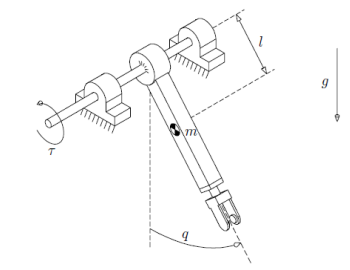
\includegraphics[width=0.32\linewidth,height=0.32\textheight,keepaspectratio]{attachments/Esquema de la carga.png}
    \caption{Esquema del brazo manipulador y de su coordenada articular $q$.}
    \label{fig:esquema-carga}
\end{figure}

Las ecuaciones que describen este sistema son:
\begin{align}
    J_l \frac{d\omega_l(t)}{dt} & = T_q(t) - b_l \omega_l(t) - T_l(t) \label{eq:carga1} \\
    \frac{d\theta_l(t)}{dt}  & \equiv \omega_l(t)  \label{eq:Carga2}
\end{align}

donde, a su vez, los parámetros $T_l(t)$ y $\theta_l(t)$ cumplen también a las siguientes ecuaciones:
\begin{align}
    T_{l}(t) & = gk_{l}\sin\big(\theta_{l}(t)\big) + T_{dl}(t)
\label{eq:torque-carga} \\
    \theta_{l}(t) & = \int_{0}^{t} \omega_{l}(\xi) \, d\xi + \theta_{l}(0)
\notag
\end{align}

Los valores numéricos de las magnitudes físicas son como se menciona a continuación:

\begin{table}[!htbp]
    \centering
    \caption{Coeficientes y datos del modelo base de la carga.}
    \label{tab:parametros_carga}
    % \small
    \begin{tabular}{lcc}
        \hline
        \textbf{Parámetro} & \textbf{Valor} & \textbf{Magnitud (Unidad)} \\
        \hline
        $b_l$ & $\approx 0.1 \pm 0.03$ & $\mathrm{Nm / (rad/s)}$ \\
        $m$ & $1.0$ & $\mathrm{kg}$ \\
        $l_{cm}$ & $0.25$ & $\mathrm{m}$ \\
        $J_{cm}$ & $0.0208$ & $\mathrm{kg \cdot m^{2}}$ \\
        $l_l$ & $0.50$ & $\mathrm{m}$ \\
        $m_l$ & $[0 \dots 1.5]$ & $\mathrm{kg}$ \\
        $J_l$ & $0.0833 + [0 \dots 0.375]$ & $\mathrm{kg \cdot m^{2}}$ \\
        $k_l$ & $0.25 + [0 \dots 0.75]$ & $\mathrm{kg \cdot m}$ \\
        $g$ & $9.80665$ & $\mathrm{m/s^2}$ \\
        \hline
    \end{tabular}
\end{table}

\begin{table}[htbp]
    \centering
    \caption{Especificaciones de operación de la carga.}
    \label{tab:parametros_carga}
    % \small
    \begin{tabular}{lcc}
        \hline
        \textbf{Parámetro} & \textbf{Valor} & \textbf{Magnitud (Unidad)} \\
        \hline
        $T_{ld}$ & $\approx 0 \pm 5.0$ & $\mathrm{Nm}$ \\
        \hline
    \end{tabular}
\end{table}


% ---------------------------------------------------------------------------- %
\subsection{Tren de Trasmisión}

El sistema del Tren de Trasmisión consta en una caja reductora reversible con sistema de engranajes planetarios, asumiendo acoplamiento rígido (sin elasticidad torsional y sin juego, holgura o “backlash”); momento de inercia equivalente y pérdidas de energía por fricción interna, reflejados al eje de entrada y considerados junto con el sistema de la PMSM (Máquina Eléctrica).

La ecuación que rige al sistema es:

\begin{align}
    \omega_{l}(t)  & = \frac{1}{r} \omega_{m}(t) \label{Transmision1}\\
    T_{q}(t)  & = r \cdot T_{d}(t)  \label{Transmision2}
\end{align}

Luego, los coeficientes del sistema y las especificaciones de operación del tren de transmisión tienen los siguientes valores:
\begin{table}[htbp]
    \centering
    \caption{Coeficientes y datos del modelo base del tren de transmisión.}
    \label{tab:parametros_carga}
    % \small
    \begin{tabular}{lcc}
        \hline
        \textbf{Parámetro} & \textbf{Valor} & \textbf{Magnitud (Unidad)} \\
        \hline
        $r$ & $120.0:1.0$ & $\mathrm{adim}$ \\
        \hline
    \end{tabular}
\end{table}

\begin{table}[htbp]
    \centering
    \caption{Especificaciones de operación del tren de trasmisión.}
    \label{tab:parametros_carga}
    % \small
    \begin{tabular}{lcc}
        \hline
        \textbf{Parámetro} & \textbf{Valor} & \textbf{Magnitud (Unidad)} \\
        \hline
        $n_{l \; \mathrm{nom}}$ & $60$ & $\mathrm{rpm}$ \\
        $T_{q \; \mathrm{nom}}$ & $17.0$ & $\mathrm{Nm}$ \\
        $T_{q \; \mathrm{max}}$ & $45.0$ & $\mathrm{Nm}$ \\
        \hline
    \end{tabular}
\end{table}


Estos parámetros no deberán ser superados durante el periodo de trabajo.

% ---------------------------------------------------------------------------- %
\subsection{PMSM (Máquina Eléctrica)}
La Máquina Síncrona de Imanes Permanentes (PMSM) cuenta con estátor simétrico y equilibrado, con bornes de fase $abc$ conectadas externamente en estrella (Y), con centro O flotante (no accesible) y bornes de línea $ABC$ accesibles desde el inversor electrónico trifásico.

Las especificaciones de operación de este sistema son:

\begin{table}[htbp]
    \centering
    \caption{Especificaciones de operación del motor en bornes de fases $abcs$ de estator (valores límite, no sobrepasar).}
    \label{tab:parametros_carga}
  %   \small
    \begin{tabular}{lcc}
        \hline
        \textbf{Parámetro} & \textbf{Valor} & \textbf{Magnitud (Unidad)} \\
        \hline
        $n_{m \; \mathrm{nom}}$ & $6600$ & $\mathrm{rpm}$ \\
        $V_{sl \; \mathrm{nom}}$ & $30.0$ & $\mathrm{V_{ca \; RMS}}$ \\
        $I_{s \; \mathrm{nom}}$ & $0.4$ & $\mathrm{A_{ca \; RMS}}$ \\
        $I_{s \; \mathrm{max}}$ & $2.0$ & $\mathrm{A_{ca \; RMS}}$ \\
        $T_{s \; \mathrm{max}}^{\circ}$ & $115.0$ & $\mathrm{{}^{\circ}C}$ \\
        $T_{\mathrm{amb}}$ & $[-15 ... 40]$ & $\mathrm{{}^{\circ}C}$ \\
        \hline
    \end{tabular}
\end{table}

La PMSM se modela mediante tres subsistemas acoplados.




\subsubsection{Subsistema Mecánico}
Las ecuaciones que de este sistema son similares a las del sistema de la carga:

\begin{align}
    J_m \frac{d\omega_m(t)}{dt} &= T_m(t) - b_m \omega_m(t) - T_d(t) \label{SubMec1}\\
    \frac{d\theta_m(t)}{dt} &\equiv \omega_m(t)  \label{SubMec2}
\end{align}

donde $\theta_m$ también puede calcularse como:
\[
\theta_{m}(t) = \int_{0}^{t} \omega_{m}(\xi) \, d\xi + \theta_{m}(0) 
\]

Los valores de los coeficientes de este subsistema son:
\begin{table}[htbp]
    \centering
    \caption{Coeficientes y datos del subsistema mecánico.}
    \label{tab:parametros_carga}
%    \small
    \begin{tabular}{lcc}
        \hline
        \textbf{Parámetro} & \textbf{Valor} & \textbf{Magnitud (Unidad)} \\
        \hline
        $J_m$ & $\approx 14.0 \times 10^{-6}$ & $\mathrm{\mathrm{kg \; m}}$ \\
        $b_m$ & $\approx 15.0 \times 10^{-6}$ & $\mathrm{\mathrm{\frac{Nm}{rad/s}}}$ \\
        \hline
    \end{tabular}
\end{table}

\subsubsection{Subsistema electromagnético}
El subsistema electromagnético responde a un modelo idealizado equivalente en coordenadas $dq0^r$ "fijas" al rotor. Para el estudio de este subsistema se utiliza la Transformación de Park en el circuito del estator estacionario. Teniendo en cuenta que las siguientes ecuaciones trabajan en el espacio de Park, el subsistema electromagnético puede ser modelado con las siguientes expresiones matemáticas:

\begin{itemize}
    \item Relación entre el espacio inercial y el espacio de Park
    \begin{align}
    \frac{d\theta_{r}(t)}{dt}  & \equiv \omega_{r}(t) \label{SubElec1}\\
    \theta_{r}(t)  & \equiv P_{p} \theta_{m}(t)  \label{SubElec2}
    \end{align}
    \item Balance de tensiones eléctricas equivalentes de estator y cálculo del torque electromagnético producido por el motor
    \begin{align}
        T_{m}(t) &  = \frac{3}{2}P_{p} \lambda_{m}^{'r} i_{qs}^{r}(t) + \frac{3}{2} P_{p} \Big( L_{d} - L_{q} \Big) i_{qs}^{r}(t) i_{ds}^{r}(t) \label{SubElec3} \\
        v_{qs}^{r}(t) & = R_{s} \Big( T_{s}^{\circ} (t) \Big) i_{qs}^{r}(t) + L_{q} \frac{di_{qs}^{r}(t)}{dt}  + \Big[ \lambda_{m}^{'r} + L_{d} i_{ds}^{r}(t) \Big] \omega_{r}(t)\label{SubElec4} \\
        v_{ds}^{r}(t) & = R_{s} \Big( T_{s}^{\circ} (t) \Big) i_{ds}^{r}(t) + L_{d} \frac{di_{ds}^{r}(t)}{dt} - L_{q}i_{qs}^{r}(t) \omega_{r}(t)   \label{SubElec5}\\
        v_{0s}^{r}(t) & = R_{s} \Big( T_{s}^{\circ} (t) \Big) i_{0s}^{r}(t) + L_{ls} \frac{di_{0s}^{r}(t)}{dt} \label{SubElec6}
    \end{align}
\end{itemize}

Los valores de los coeficientes de este subsistema son:

\begin{table}[htbp]
    \centering
    \caption{Coeficientes y datos del subsistema electromagnético.}
    \label{tab:parametros_carga}
 %   \small
    \begin{tabular}{lcc}
        \hline
        \textbf{Parámetro} & \textbf{Valor} & \textbf{Magnitud (Unidad)} \\
        \hline
        $P_p$ & $3$ & Pares de Polos \\
        $\lambda_{m}^{'r}$ & $0.016$ & $\mathrm{\frac{V}{rad/s}}$ \\
        $L_q$ & $5.8$ & $\mathrm{mH}$ \\
        $L_s$ & $6.6$ & $\mathrm{mH}$ \\
        $L_{ls}$ & $0.8$ & $\mathrm{mH}$ \\
        \hline
    \end{tabular}
\end{table}

\subsubsection{Subsistema Térmico}
El subsistema térmico consta de un modelo simplificado equivalente de primer orden, considerando sólo pérdidas eléctricas resistivas por efecto Joule (calor) en bobinado de estator, despreciando pérdidas magnéticas en el núcleo; transferencia de calor al ambiente solo por conducción y convección natural y sin ventilación forzada.

Las ecuaciones que representan la variación del valor de las resistencias de bobinado y las pérdidas por calor se expresan como:

\begin{align}
    R_{s}(T_{s}^{\circ}(t)) & = R_{sREF} \Big(1 + \alpha_{Cu} (T_{s}^{\circ}(t) - T_{sREF}^{\circ}) \Big) \label{SubTerm1}\\
    P_{s \; \text{perdida}}(t)  & = R_{s}(T_{s}^{\circ}(t)) \Big( i_{as}^{2}(t) + i_{bs}^{2}(t) + i_{cs}^{2}(t) \Big)
\label{SubTerm2} \\
     & = R_{s}(T_{s}^{\circ}(t)) \frac{3}{2} \Big( i_{qs}^{r\;2}(t) + i_{ds}^{r\;2}(t) + 2i_{0s}^{r\;2}(t) \Big)
\label{SubTerm3} \\
     & = C_{ts} \frac{dT_{s}^{\circ}(t)}{dt} +  \frac{T_{s}^{\circ}(t) - T_{amb}^{\circ}(t)}{R_{ts-amb}}
\label{eq:balance-termico}
\end{align}

Como se puede ver, las ecuaciones \eqref{SubTerm2} y \eqref{SubTerm3} son las formas de calcular las pérdidas de potencia por calor debido a efecto Jouls — ya sea teniendo en cuenta las corrientes de bornes o las corrientes virtuales del espacio de Park — y también son equivalentes a la perdida de potencia deducida por el balance térmico de la PMSM. Más adelante se hablará de la Transformada de Park, pero resulta coherente que el cambio variables de tensión de bornes (tensiones abc) y tensiones virtuales (tensiones $dq0$) expresen la misma potencia, puesto que ambos representan el mismo fenómeno (no se crea ni destruye energía).

Los valores de los coeficiente son:

\begin{table}[htbp]
    \centering
    \caption{Coeficientes y datos del subsistema térmico.}
    \label{tab:parametros_carga}
  %  \small
    \begin{tabular}{lcc}
        \hline
        \textbf{Parámetro} & \textbf{Valor} & \textbf{Magnitud (Unidad)} \\
        \hline
        $R_s$ & $\approx 1.02$ & $\Omega$ \\
        $\alpha_{Cu}$ & $3.9 \times 10^{-3}$ & $\mathrm{\frac{1}{{}^\circ C}}$ \\
        $C_{ts}$ & $0.818$ & $\mathrm{\frac{W}{{}^\circ C/s}}$ \\
        $R_{ts-amb}$ & $146.7$ & $\mathrm{\frac{{}^\circ C}{W}}$ \\
        \hline
    \end{tabular}
\end{table}

En el modelo térmico se adopta una resistencia de referencia del bobinado $R_{sREF}=1{,}02\,\Omega$ a una temperatura $T_{sREF}^{\circ}=20\,^\circ\mathrm{C}$.

% ---------------------------------------------------------------------------- %
\subsection{Inversor Trifásico de Alimentación}
El sistema del Inversor trifásico de 4 cuadrantes (regenerativo), consiste en un puente trifásico con llaves electrónicas semiconductoras  alimentado desde fuente de CC de tensión constante, conmutado con modulación de ancho de pulso, PWM.

Se asume inicialmente el Modulador de tensión trifásico (vectorial) sin límite de tensión, con respuesta ideal $G(s) \equiv 1$ (filtro “pasatodo”, ganancia unitaria y ancho de banda “infinito”). En un estudio posterior, esta hipótesis será modificada.

Las ecuaciones que modelan este sistema son:

\begin{align}
    \frac{d\theta_{ev}(t)}{dt}  & \equiv 2\pi f_{e}(t) \equiv \omega_{e}(t)
\label{eq:angulo-inversor} \\
    \delta(t)  & \equiv \theta_{ev}(t) - \theta_{r}(t)
\label{eq:desfase-inversor} \\
    v_{as}(t)  & \cong \sqrt{ 2 } \frac{V_{sl}(t)}{\sqrt{ 3 }} \cos \Big( \theta_{ev}(t) \Big)
\label{eq:tension-fase-a} \\
    v_{bs}(t) &  \cong \sqrt{ 2 } \frac{V_{sl}(t)}{\sqrt{ 3 }} \cos \Big( \theta_{ev}(t) - \frac{2\pi}{3} \Big)
\label{eq:tension-fase-b} \\
    v_{cs}(t) &  \cong \sqrt{ 2 } \frac{V_{sl}(t)}{\sqrt{ 3 }} \cos \Big( \theta_{ev}(t) + \frac{2\pi}{3}  \Big)
\label{eq:tension-fase-c}
\end{align}

De aquí, se puede apreciar como las tensiones que alimentan el motor son controladas única y exclusivamente con los parámetros $V_{sl}(t)$ y $\omega_e(t)\equiv 2\pi \; f_e(t)$, los cuales son los parámetros manipulados por el operador (nosotros).

Además, aparece $\delta(t)$ — ángulo de desfasaje electromagnético de rotor — el cual representa el desfasaje instantáneo relativo entre la coordenada eléctrica sincrónica $\theta_{ev}$ (tensión de fase $a$ del estator) y la coordenada eléctrica fija a rotor $\theta_r$ (respecto al espacio $dq0^r$). Esta última depende del torque electromagnético.

\begin{table}[htbp]
    \centering
    \caption{Especificaciones de operación del sistema de Alimentación.}
    \label{tab:parametros_carga}
   % \small
    \begin{tabular}{lcc}
        \hline
        \textbf{Parámetro} & \textbf{Valor} & \textbf{Magnitud (Unidad)} \\
        \hline
        $V_{sl}$ & $[0.0 ... 48]$ & $\mathrm{V_{ca \; RMS}}$ \\
        $f_e$ & $[-330 ... 0 ... +330]$ & $\mathrm{Hz}$ \\
        \hline
    \end{tabular}
\end{table}

Se debe tener en cuenta que el signo de $f_e$ ($\pm$) determina la secuencia de fases positiva (abc) ó negativa (acb) y por consiguiente, el sentido de giro del campo magnético rodante y del rotor.

% ---------------------------------------------------------------------------- %
\subsection{Sensores de Retroalimentación}
Para la medición y acondicionamiento de las señales de realimentación indispensables para el lazo cerrado, el sistema incorpora los siguientes dispositivos físicos:

\begin{itemize}
    \item \textbf{Un (1) sensor de posición angular:} Consiste en un codificador incremental (\textit{encoder}) montado en el eje motor. Teniendo un proceso de \textit{homing} y decodificación ideal, registra la posición angular absoluta ``rectificada'' $\theta_m(t)$. Esta variable se vincula a la coordenada articular de la carga mediante la relación mecánica $\theta_l(t) = \frac{1}{r} \theta_m(t)$, estableciéndose un ajuste de origen tal que $\theta_m \equiv 0$ cuando $\theta_l \equiv 0$.
    \item \textbf{Tres (3) sensores de corriente instantánea:} Consisten en amperímetros montados en la salida trifásica del inversor electrónico hacia los bornes del estator. Miden las corrientes reales de fase $i_a(t)$, $i_b(t)$ e $i_c(t)$, las cuales permiten la reconstrucción de las corrientes virtuales del espacio de Park ($i_{qs}^r$, $i_{ds}^r$, $i_{0s}^r$) mediante la Transformada de Park.
    \item \textbf{Un (1) sensor de temperatura:} Consiste en un sensor instalado en el bobinado del estator. Registra la variable térmica $T_s^\circ(t)$ empleada para el monitoreo de calentamiento, la protección ante sobretemperaturas y el cálculo constante de la variación de la resistencia del estator $R_s(T_s^\circ(t))$.
\end{itemize}

%\begin{quote}
 %   \textbf{Nota sobre el modelo de respuesta:} Inicialmente, para el análisis dinámico a lazo abierto y el diseño de la ley de control por retroalimentación, se asume un comportamiento ideal para todos los transductores, caracterizado por una función de transferencia unitaria $G(s) \equiv 1$ (ganancia unitaria, filtro ``pasa todo'' y ancho de banda infinito).
%\end{quote}

\subsection{Espacio de Park}

En la década de 1920, R.H. Park introdujo una nueva forma de analizar máquinas eléctricas: formuló un cambio de variables que reemplaza, de forma efectiva, las variables asociadas a los devanados del estator de una máquina síncrona por variables asociadas a devanados ficticios que rotan a la velocidad angular eléctrica del rotor.

La transformada de Park tiene la propiedad única de eliminar las inductancias dependientes de la posición del rotor en las ecuaciones de tensión de las máquinas síncronas, las cuales surgen debido a circuitos eléctricos con movimiento relativo entre sí y a circuitos con diferentes valores de reluctancia magnética.

La Figura~\ref{fig:ejes-transformada-park} muestra los dos conjuntos de ejes de la transformación. Las variables $f_{as}$, $f_{bs}$ y $f_{cs}$ se asocian a tres ejes fijos separados $120^\circ$ entre sí. Las componentes $f_{ds}$ y $f_{qs}$ se asocian a dos ejes ortogonales que giran a la velocidad angular eléctrica $\omega$ del marco elegido.

\noindent\begin{minipage}{\linewidth}
  \begingroup
    \centering
    \captionsetup{type=figure}
    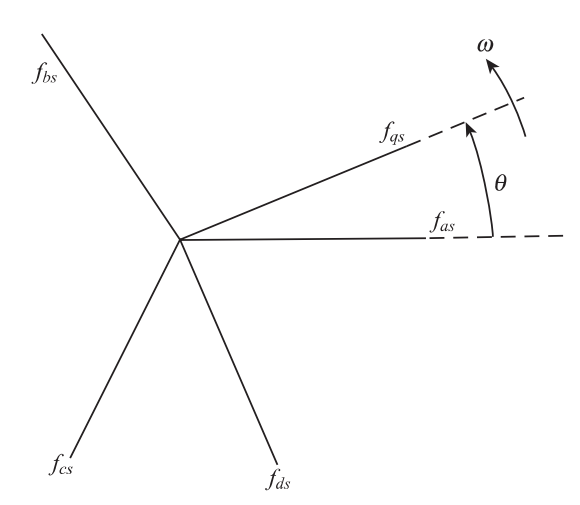
\includegraphics[width=0.42\linewidth,height=0.26\textheight,keepaspectratio]{attachments/TransformadaDePark.png}
    \caption{Ejes trifásicos $abc$ y ejes giratorios $dq$ de la transformada de Park.}
    \label{fig:ejes-transformada-park}
    \par
  \endgroup

  \medskip
  La Tabla~\ref{tab:reference_frames} resume los marcos de referencia más usados y la notación de sus variables y matrices de transformación. La elección del marco determina la velocidad $\omega$ de los ejes $dq$.

  \medskip
  \begingroup
    \centering
    \captionsetup{type=table}
    \renewcommand{\arraystretch}{1.5} % Da respiro vertical a las filas
    \begin{tabular}{@{}llcc@{}}
        \toprule
        & & \multicolumn{2}{c}{Notation} \\ \cmidrule(l){3-4}
        \begin{tabular}[c]{@{}l@{}}Reference-\\ Frame Speed\end{tabular} & 
        \multicolumn{1}{c}{Interpretation} & 
        Variables & 
        Transformation \\
        \midrule
        
        $\omega$ (unspecified) & 
        \begin{tabular}[c]{@{}c@{}}Stationary circuit variables referred to an \\ arbitrary reference frame\end{tabular} & 
        \begin{tabular}[c]{@{}c@{}}$\mathbf{f}_{dq0s}$ or $f_{ds}, f_{qs},$\\ $f_{0s}$\end{tabular} & 
        $\mathbf{K}_s$ \\
        
        $0$ & 
        \begin{tabular}[c]{@{}c@{}}Stationary circuit variables referred to a \\ stationary reference frame\end{tabular} & 
        \begin{tabular}[c]{@{}c@{}}$\mathbf{f}^s_{dq0s}$ or\\ $f^s_{ds}, f^s_{qs}, f_{0s}$\end{tabular} & 
        $\mathbf{K}^s_s$ \\
        
        $\omega_r$ & 
        \begin{tabular}[c]{@{}c@{}}Stationary circuit variables referred to a \\ reference frame fixed in the rotor\end{tabular} & 
        \begin{tabular}[c]{@{}c@{}}$\mathbf{f}^r_{dq0s}$ or\\ $f^r_{ds}, f^r_{qs}, f_{0s}$\end{tabular} & 
        $\mathbf{K}^r_s$ \\
        
        $\omega_e$ & 
        \begin{tabular}[c]{@{}c@{}}Stationary circuit variables referred to a \\ synchronously rotating reference frame\end{tabular} & 
        \begin{tabular}[c]{@{}c@{}}$\mathbf{f}^e_{dq0s}$ or \\ $f^e_{ds}, f^e_{qs},, f_{0s}$\end{tabular} & 
        $\mathbf{K}^e_s$ \\
        
        \bottomrule
    \end{tabular}
    \caption{Marcos de referencia de uso frecuente. Adaptado de \cite{krause2013electric}.}
    \label{tab:reference_frames}
    \par
  \endgroup
\end{minipage}

En este informe se adopta el marco ligado al rotor de la Tabla~\ref{tab:reference_frames}, con $\omega=\omega_r$. En ese marco, la transformada directa de Park expresa las tensiones de fase $abc$ en componentes $dq0$.

\begin{equation}
\label{eq:park-directa}
\begin{bmatrix}
    v_d \\ v_q \\v_0
\end{bmatrix} 
=
\frac{2}{3} 
\begin{bmatrix}
    \sin \theta & \sin\left(\theta - \frac{2\pi}{3}\right) & \sin\left(\theta + \frac{2\pi}{3}\right) \\[1em]
    \cos \theta & \cos\left(\theta - \frac{2\pi}{3}\right) & \cos\left(\theta + \frac{2\pi}{3}\right) \\[1em]
    \frac{1}{2} & \frac{1}{2} & \frac{1}{2}
\end{bmatrix}
\begin{bmatrix}
    v_a \\ v_b \\v_c
\end{bmatrix} 
\end{equation}

La transformada inversa de Park permite obtener las tensiones de fase $abc$ a partir de sus componentes $dq0$.

\begin{equation}
\label{eq:park-inversa}
\begin{bmatrix}
    v_a \\ v_b \\v_c
\end{bmatrix} 
=
\begin{bmatrix}
    \sin \theta & \cos \theta  & 1 \\[1em]
     \sin\left(\theta - \frac{2\pi}{3}\right) & \cos\left(\theta - \frac{2\pi}{3}\right) & 1 \\[1em]
     \sin\left(\theta + \frac{2\pi}{3}\right) & \cos\left(\theta + \frac{2\pi}{3}\right) & 1
\end{bmatrix}
\begin{bmatrix}
    v_d \\ v_q \\v_0
\end{bmatrix} 
\end{equation}

Para mantener la notación de manera unificada, se utiliza el orden $dq0$ el cual es también utilizado en los bloques de los modelos en Simulink, de manera opuesta a como algunas otras bibliografias utilizan el orden $dq0$. Este cambio de orden en las variables virtuales no provoca diferencia en los resultados de modelado, siempre y cuando se considere la transformada (directa o inversa) de forma tal que respete el orden de la notación adoptada.

En este estudio, se hace uso de la Transformada de Park implementada con una alineación de la fase $a$ cn el eje en cuadratura $q$ dado por el hecho de que se utilizan cosenos para calcular las variables en cuadratura. 

\clearpage
% ============================================================================= %
\section{Modelado, Análisis y Simulación dinámica del SISTEMA FÍSICO a “Lazo
Abierto” (Sin Controlador externo de Movimiento)}

% ---------------------------------------------------------------------------- %
\subsection{Modelo Matemático Equivalente del Subsistema Mecánico Completo, referido al Eje Motor.}

En lo que a fenómenos mecánicos respecta, se deben analizar las ecuaciones de la carga, del tren de transmisión y el Subsistema Mecánico de la PMSM, las respectivas ecuaciones \eqref{eq:carga1}, \eqref{eq:Carga2},
\eqref{Transmision1},
\eqref{Transmision2}, \eqref{SubMec1} y \eqref{SubMec2}.

Si se utilizarán estas ecuaciones, las cuales forman un sistema de 6 ecuaciones diferenciales acopladas de primer orden, se podría llegar a un grafo de la siguiente forma:

\begin{figure}[!htbp]
    \centering
    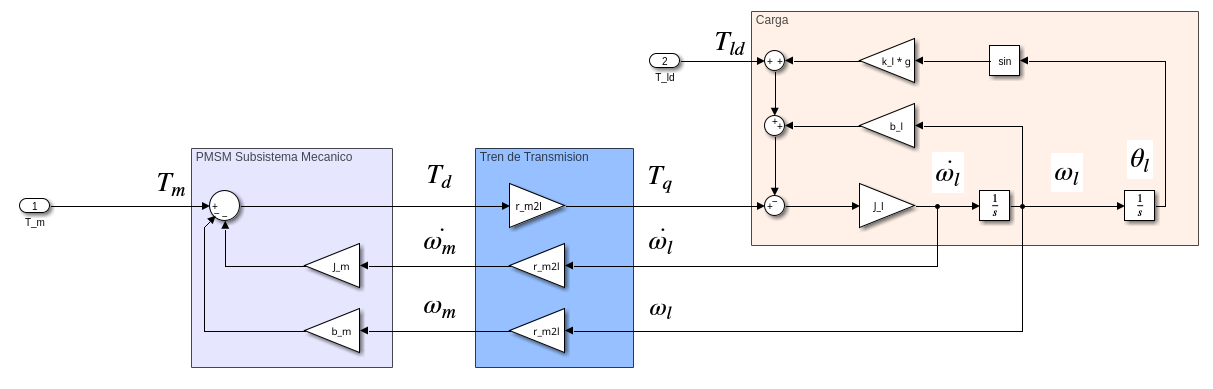
\includegraphics[width=\linewidth,height=0.72\textheight,keepaspectratio]{attachments/Sistema_Carga_Trasmision_SubMecPMSM.png}
    \caption{Grafo de los sistemas de Carga, Transmisión y Subsistema Mecánico}
\end{figure}

Al combinar los balances de torque de la carga y del motor
\eqref{eq:carga1} y \eqref{SubMec1} con las relaciones del reductor
\eqref{Transmision1} y \eqref{Transmision2}, se elimina el torque interno
$T_d$ y se obtiene un modelo mecánico equivalente referido al eje motor.
El modelo se expresa mediante dos ecuaciones diferenciales acopladas
de primer orden para $\theta_m$ y $\omega_m$. La dependencia senoidal
del torque gravitatorio respecto de $\theta_m$ conserva la no linealidad
del modelo.

Partiendo de la ecuación \eqref{eq:carga1} y despejando $T_q$ se puede llegar a la expresión:
\[
T_{q}(t) = J_{l} \frac{d\omega_{l}(t)}{dt} + b_{l}\omega_{l}(t) + k_{l}g\sin \big(\theta_{l}(t)\big) +T_{dl}(t)
\]

Se realizan los reemplazos $\omega_l=\frac{1}{r}\omega_m$, $\theta_l=\frac{1}{r}\theta_m$ y $T_q=r \; T_d$ y se reemplaza $T_d$ en la ecuación \eqref{SubMec1}, dejando:

\[
J_{m} \frac{d\omega_{m}(t)}{dt} = T_{m}(t) - b_{m}\omega_{m}(t) - \frac{1}{r} \left[ \frac{J_{l}}{r} \frac{d\omega_{m}(t)}{dt} + \frac{b_{l}}{r} \omega_{m}(t) + k_{l} g \sin \left( \frac{1}{r} \theta_{m}(t) \right) + T_{dl}(t) \right]
\]

Despejando, se puede llegar a:

\begin{equation}
\label{eq:mecanica-equivalente}
\underbrace{ \left( J_{m}+\frac{J_{l}}{r^{2}} \right)  }_{ J_{eq} } \frac{d\omega_{m}(t)}{dt} = T_{m}(t) - \underbrace{ \left( b_{m} + \frac{b_{l}}{r^{2}} \right) }_{ b_{eq} }  \omega_{m}(t) -  \frac{1}{r} T_{dl}(t)  - \frac{k_{l}g}{r} \sin \left(  \frac{1}{r} \theta_{m}(t) \right)
\end{equation}

Definimos entonces como parámetros equivalentes a:

\begin{itemize}
    \item$J_{eq}$: Momento de Inercia Equivalente del Sistema Mecánico Equivalente.
    \item$b_{eq}$: Amortiguamiento Viscoso Equivalente del Sistema Mecánico Equivalente.
\end{itemize}

\begin{table}[htbp]
    \centering
    \caption{Parámetros Equivalentes del Sistema Mecánico Equivalente}
    \small
    \begin{tabular}{lcc}
        \hline
        \textbf{Parámetro Equivalente} & \textbf{Valor} & \textbf{Magnitud (Unidad)} \\
        \hline
        $J_{eq}$ & $45.826 \times 10^{-6}$ & $\mathrm{\mathrm{kg \; m^2}}$ \\
        $b_{eq}$ & $21.944 \times 10^{-6}$ & $\mathrm{\mathrm{\frac{Nm}{rad/s}}}$ \\
        \hline
    \end{tabular}
\end{table}

Con la ecuación \eqref{eq:mecanica-equivalente}, el grafo que representa a todos los fenómenos mecánicos y su sistema de ecuaciones diferenciales respectivo es:

\begin{equation}
\label{eq:modelo-mecanico}
    \begin{cases} % Inicia la llave grande
    \begin{aligned}
        \begin{bmatrix} \frac{d\theta_{m}(t)}{dt} \\ \frac{d\omega_{m}(t)}{dt} \end{bmatrix} &= 
        \begin{bmatrix} 0 & 1 \\ 0 & -\frac{b_{eq}}{J_{eq}} \end{bmatrix} 
        \begin{bmatrix} \theta_{m}(t) \\ \omega_{m}(t) \end{bmatrix} + 
        \begin{bmatrix} 0 \\ -\frac{k_{l}g}{r J_{eq}} \end{bmatrix} \sin \left( \frac{\theta_{m}(t)}{r} \right) + 
        \frac{1}{J_{eq}} \begin{bmatrix} 0 & 0 \\ 1 & -\frac{1}{r} \end{bmatrix} 
        \begin{bmatrix} T_{m}(t) \\ T_{ld}(t) \end{bmatrix} \\[10pt]
        \mathbf{y}(t) &= \begin{bmatrix} \theta_{m}(t) \\ \omega_{m}(t) \end{bmatrix}
    \end{aligned}
    \end{cases}
\end{equation}

\begin{figure}[!htbp]
    \centering
    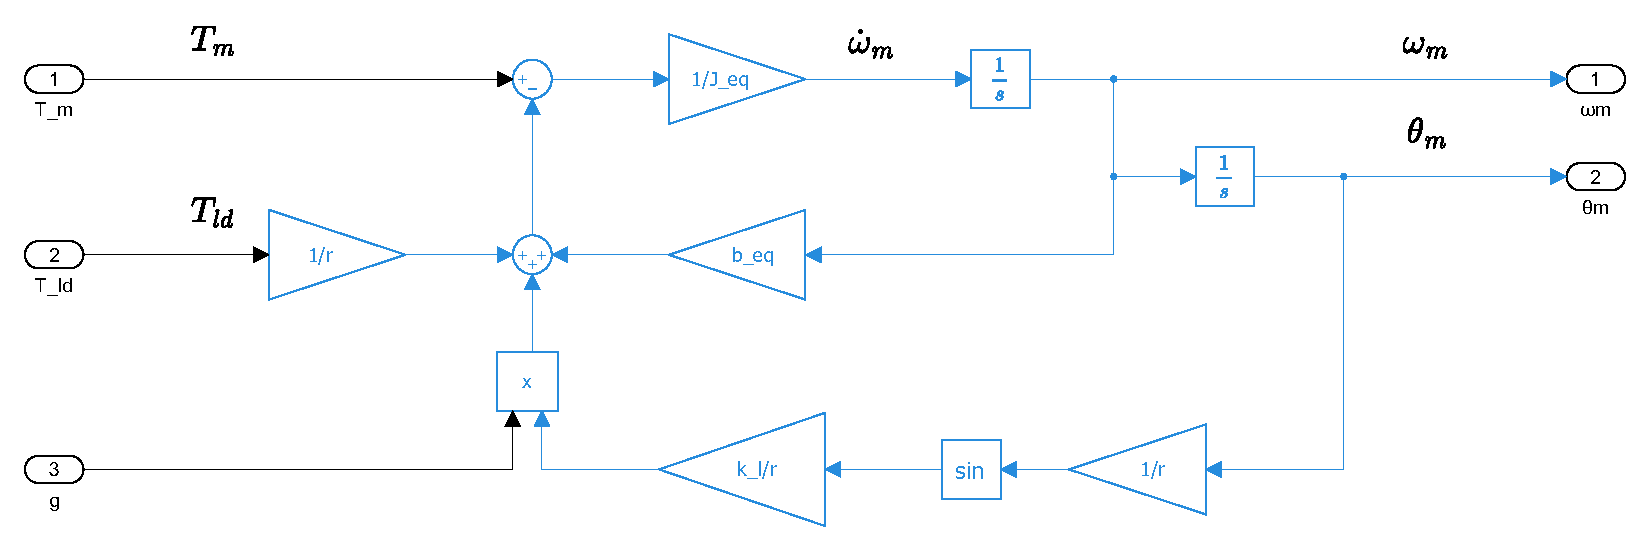
\includegraphics[width=\linewidth,height=0.32\textheight,keepaspectratio]{attachments/Subsistema Mecanico Equivalente (2).pdf}
    \par\medskip
    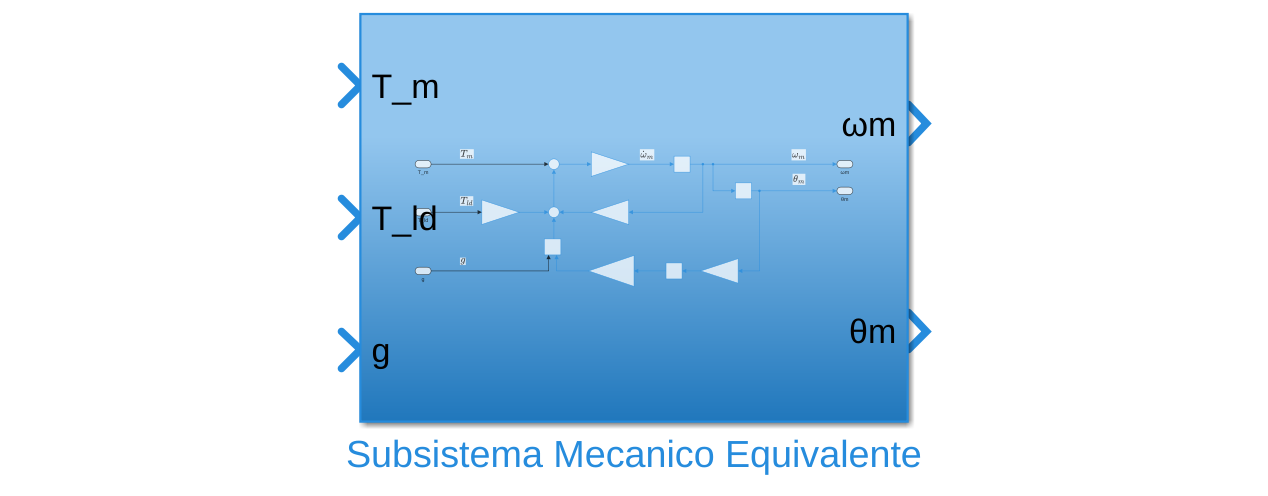
\includegraphics[width=0.36\linewidth,height=0.18\textheight,keepaspectratio]{attachments/Bloque Subsistema Mecanico Equivalente.png}
    \caption{Grafo y Bloque del Sistema Mecánico Equivalente}
\end{figure}




% ---------------------------------------------------------------------------- %
\subsection{Modelo Dinámico del Sistema Físico Completo}

% ---------------------------------------------------------------------------- %
\subsubsection{Modelo Global No Lineal}
Combinando el Sistema Mecánico Equivalente desarrollado en el inciso anterior junto con los demás sistemas de la PMSM — los previamente definidos como "Subsistema Electromagnético" y "Subsistema Térmico" respectivamente — se llega al \textbf{Modelo Global No Lineal}.

Dicha no linealidad es resultado de expresiones sinusoidales (e.g. $\sin \left( \frac{1}{r} \theta_m(t) \right)$), funciones incógnitas elevadas al cuadrado (e.g. $i_{ds}^{r \; 2}(t)$) y debido al uso de parámetros con valores locales (e.g. $b_l$). 

El Subsistema Electromagnético se desarrolla maniobrando con las corrientes virtuales de Park.  El bloque del subsistema electromagnético de la PMSM se desarrolla con las ecuaciones \eqref{SubElec3}, \eqref{SubElec4}, \eqref{SubElec5} y \eqref{SubElec6} y se despejan los términos de derivadas de las corrientes del espacio de Park para llegar a:

\begin{equation}
\label{eq:modelo-electromagnetico}
\begin{cases} % Inicia la llave grande
\begin{aligned}
        T_{m}(t) &  = \frac{3}{2}P_{p} \lambda_{m}^{'r} i_{qs}^{r}(t) + \frac{3}{2} P_{p} \Big( L_{d} - L_{q} \Big) i_{qs}^{r}(t) i_{ds}^{r}(t)  \\
        \frac{di_{ds}^{r}(t)}{dt} & = \frac{1}{L_{d}} \left[ v_{ds}^{r}(t) - R_{s} \Big( T_{s}^{\circ} (t) \Big) i_{ds}^{r}(t) + L_{q}i_{qs}^{r}(t) \omega_{r}(t)  \right]  \\
        \frac{di_{qs}^{r}(t)}{dt}  & = \frac{1}{L_{q} } \left[ v_{qs}^{r}(t) - R_{s} \Big( T_{s}^{\circ} (t) \Big) i_{qs}^{r}(t) - \big[ \lambda_{m}^{'r} + L_{d} i_{ds}^{r}(t) \big] \omega_{r}(t) \right]  \\
        \frac{di_{0s}^{r}(t)}{dt} & = \frac{1}{ L_{ls} } \left[ v_{0s}^{r}(t) - R_{s} \Big( T_{s}^{\circ} (t) \Big) i_{0s}^{r}(t) \right]
\end{aligned}
\end{cases}
\end{equation}

\begin{figure}[!htbp]
    \centering
    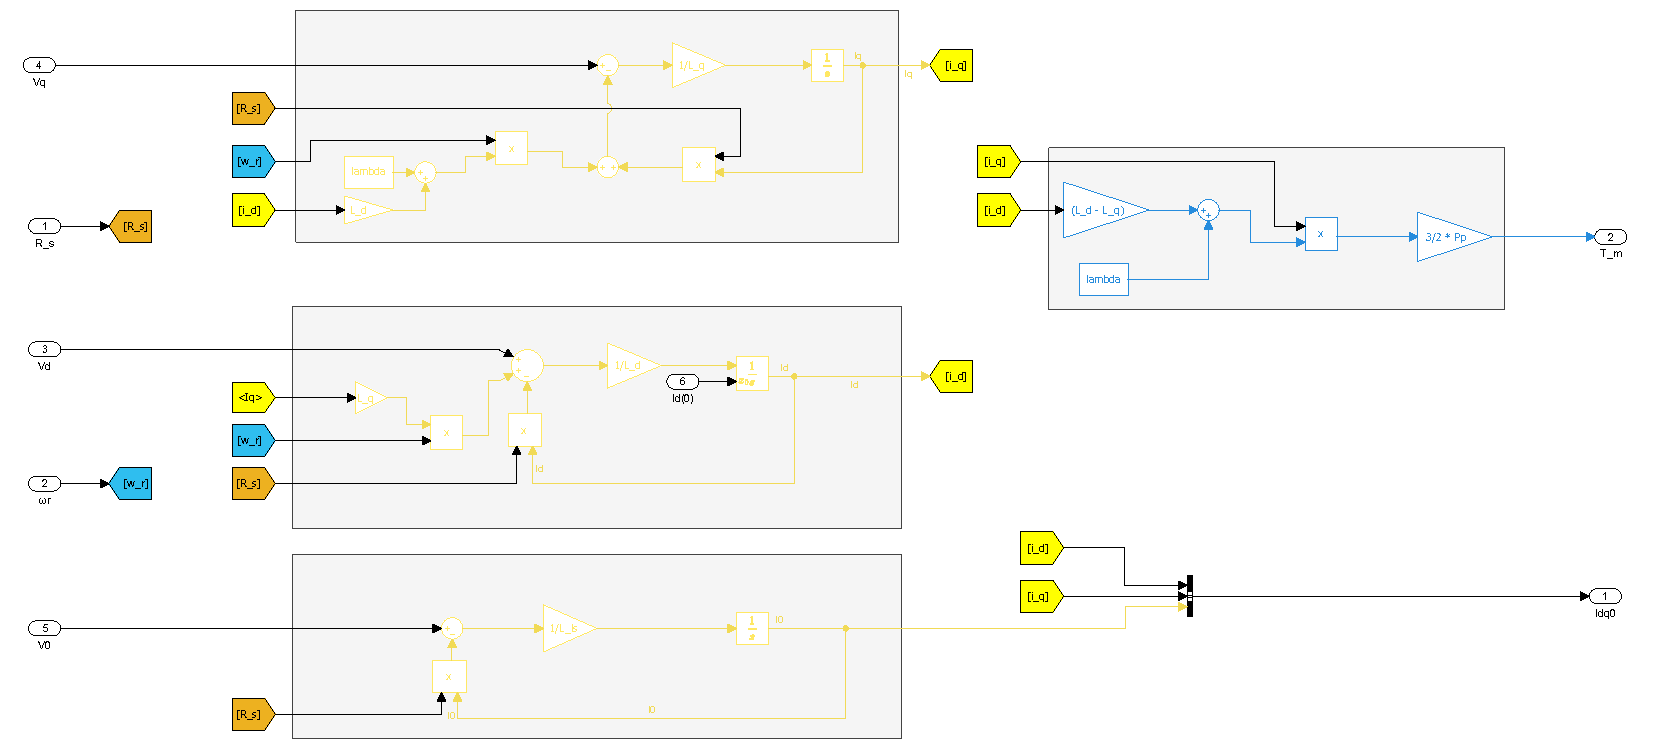
\includegraphics[width=\linewidth,height=0.32\textheight,keepaspectratio]{attachments/Subsistema Electromagnetico.pdf}
    \par\medskip
    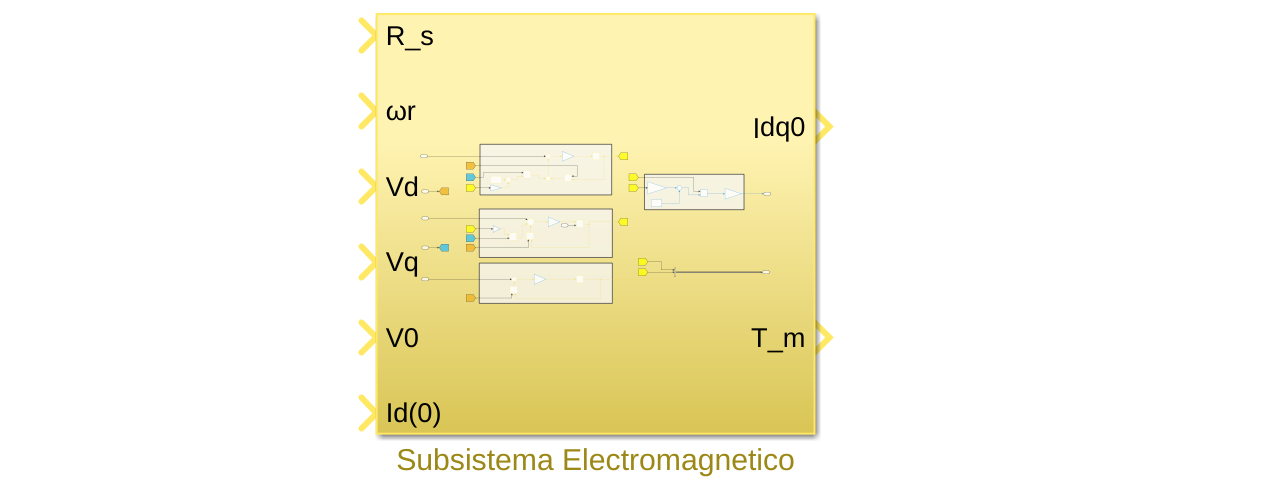
\includegraphics[width=0.36\linewidth,height=0.18\textheight,keepaspectratio]{attachments/Bloque Subsistema Electromagnetico.png}
    \caption{Grafo y Bloque del Subsistema Electromagnético de la PMSM}
\end{figure}

El planteo del subsistema térmico de la máquina PMSM se plantea como un sistema de primer orden con la diferencia de temperaturas y la potencia emanada por el motor. Además, la potencia de pérdida considera es aquella producida únicamente por efecto Joules en el bobinado del estator, despreciándose la pérdida magnética por histéresis del núcleo del motor.

Para el subsistema térmico, se utilizan las ecuaciones \eqref{SubTerm3} y \eqref{eq:balance-termico}. Primero, se despeja la derivada de la temperatura:


\begin{align}
P_{s \; \text{perdida}}(t)  & = C_{ts} \frac{dT_{s}^{\circ}(t)}{dt} + \frac{1}{R_{ts-amb}} (T_{s}^{\circ}(t) - T_{amb}^{\circ}(t))
\notag \\
\frac{dT_{s}^{\circ}(t)}{dt} & = \frac{1}{C_{ts}} \Bigg[ P_{s \; \text{perdida}}(t) - \frac{T_{s}^{\circ}(t) - T_{amb}^{\circ}(t)}{R_{ts-amb}} \Bigg]
\label{eq:temperatura-potencia}
\end{align}

Luego, se realiza el reemplazo $P_{s \; \text{perdida}}(t) = R_{s}(T_{s}^{\circ}(t)) \frac{3}{2} \Big( i_{qs}^{r\;2}(t) + i_{ds}^{r\;2}(t) + 2i_{0s}^{r\;2}(t) \Big)$ para considerar las corrientes del espacio de Park, debido a que el subsistema electromagnético se refiere a las corrientes de Park (fueron definidas como variables de estado), lo que deja la dinámica de la temperatura expresada como:

\begin{equation}
\label{eq:modelo-termico}
    \frac{dT_{s}^{\circ}(t)}{dt} = \frac{1}{C_{ts}} \Bigg[ R_{s}(T_{s}^{\circ}(t)) \frac{3}{2} \Big( i_{qs}^{r\;2}(t) + i_{ds}^{r\;2}(t) + 2i_{0s}^{r\;2}(t) \Big) - \frac{T_{s}^{\circ}(t) - T_{amb}^{\circ}(t)}{R_{ts-amb}} \Bigg]
\end{equation}

Adicionalmente, se considera la variación lineal de la resistencia del estator. Si bien la resistencia del estator $R_s$ no conforma una variable de estado como tal, es importante realizar el cálculo constante de su variación, debido a que influye en la dinámica de las corrientes de Park y la velocidad angular, las cuales si son variables de estado. Se utiliza nuevamente la relación \eqref{SubTerm1}:

\begin{equation*}
    R_{s}(T_{s}^{\circ}(t))  = R_{sREF} \Big(1 + \alpha_{Cu} (T_{s}^{\circ}(t) - T_{sREF}^{\circ}) \Big)
\end{equation*} 
\begin{figure}[!htbp]
    \centering
    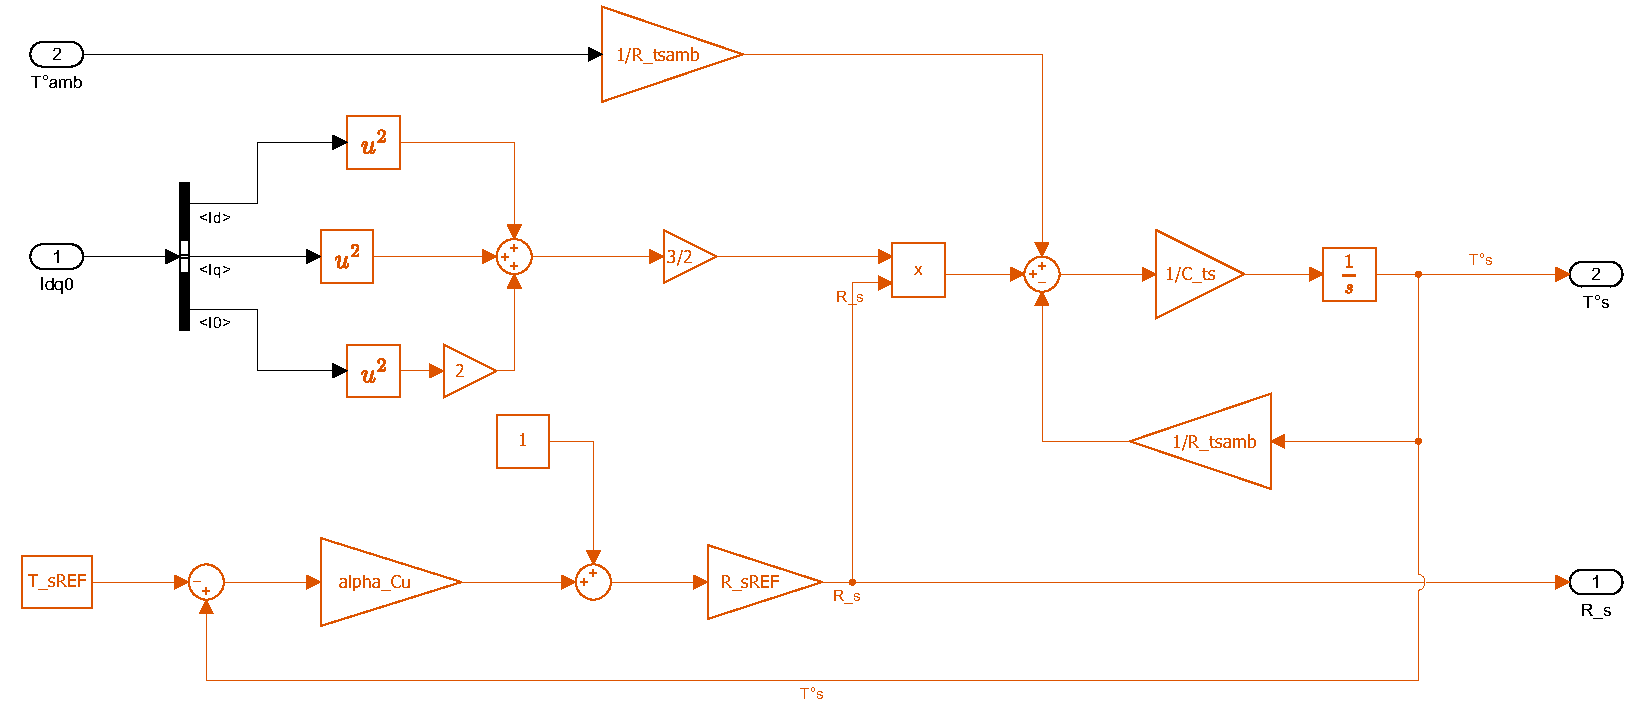
\includegraphics[width=0.9\linewidth,height=0.32\textheight,keepaspectratio]{attachments/Subsistema Termico.pdf}
    \par\medskip
    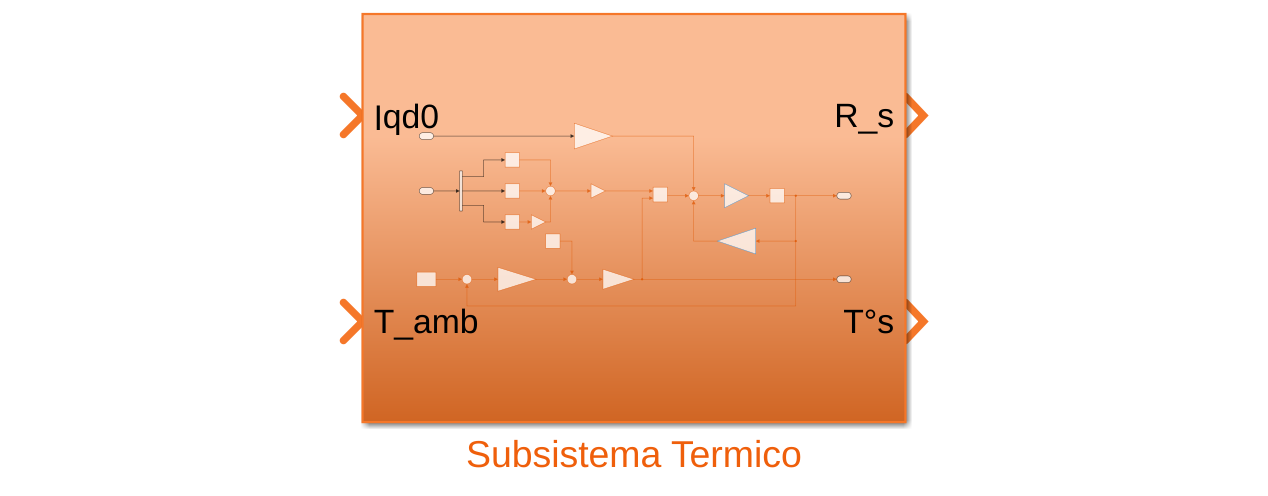
\includegraphics[width=0.36\linewidth,height=0.18\textheight,keepaspectratio]{attachments/Bloque Subsistema Termico.png}
    \caption{Diagrama interno y bloque del subsistema térmico de la PMSM.}
\end{figure}

La Figura~\ref{fig:modelo-global-nl} muestra cómo se acoplan los subsistemas mecánico equivalente, electromagnético y térmico en el modelo global no lineal.

\begin{figure}[!htbp]
    \centering
    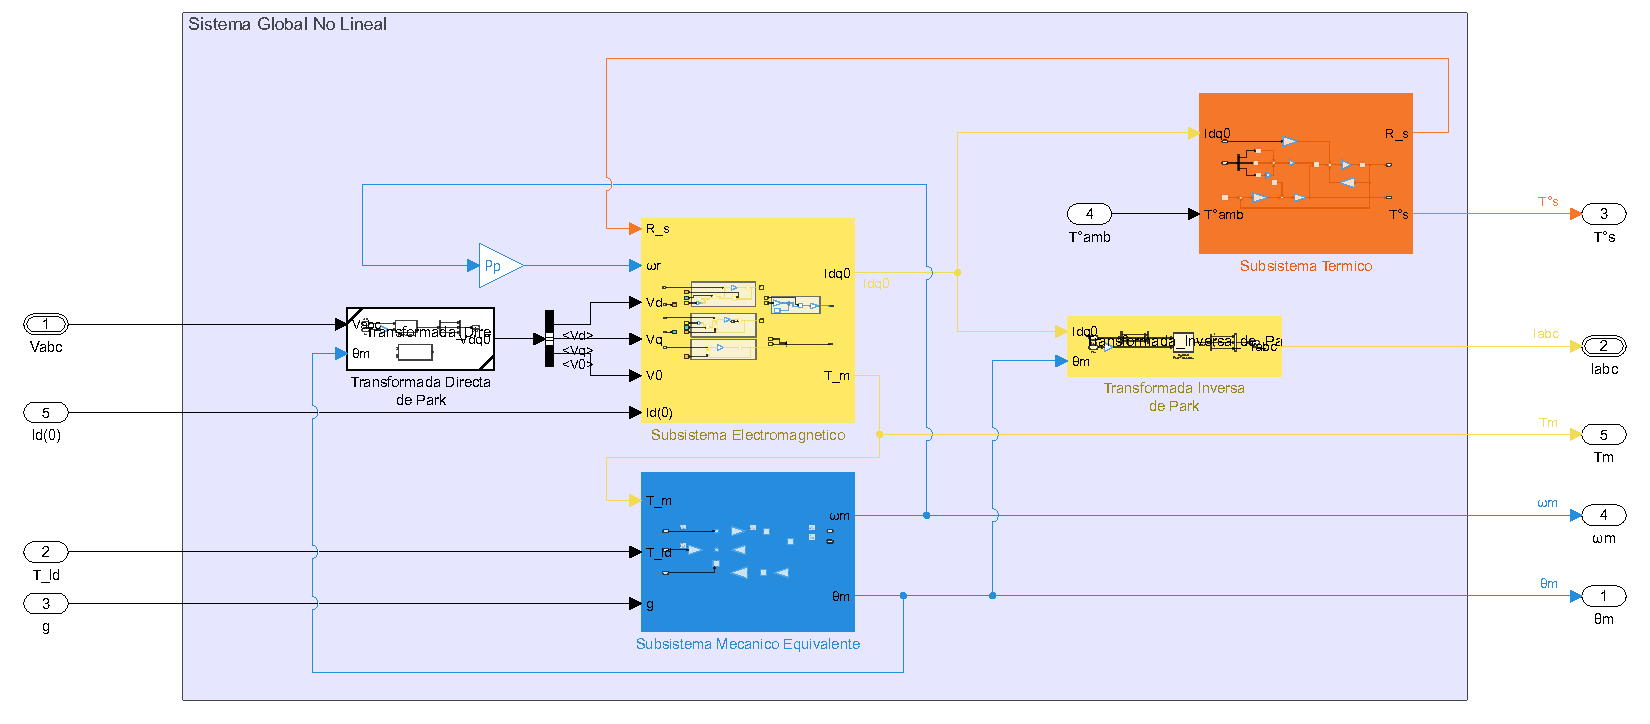
\includegraphics[width=\linewidth,height=0.72\textheight,keepaspectratio]{attachments/Bloque Modelo Global No Lineal.pdf}
    \caption{Diagrama de bloques del modelo global no lineal.}
    \label{fig:modelo-global-nl}
\end{figure}

El sistema~\eqref{eq:modelo-global-nl} reúne las seis ecuaciones diferenciales acopladas de primer orden que describen la dinámica no lineal en el espacio de estados.

\begin{equation}
\label{eq:modelo-global-nl}
    \begin{cases} % Inicia la llave grande
    \begin{aligned}
        \frac{d\theta_m(t)}{dt} & = \omega_m(t) \\
        \frac{d\omega_{m}(t)}{dt} & = \frac{1}{J_{eq}} \Bigg[ \frac{3}{2}P_{p} \lambda_{m}^{'r} i_{qs}^{r}(t) + \frac{3}{2} P_{p} \Big( L_{d} - L_{q} \Big) i_{qs}^{r}(t) i_{ds}^{r}(t) - b_{eq}  \omega_{m}(t)   - \frac{1}{r} T_{dl}(t) - \frac{k_{l}g}{r} \sin \left(  \frac{1}{r} \theta_{m}(t) \right) \Bigg]  \\
        \frac{di_{ds}^{r}(t)}{dt} & = \frac{1}{L_{d}} \left[ v_{ds}^{r}(t) - R_{s} \Big( T_{s}^{\circ} (t) \Big) i_{ds}^{r}(t) + L_{q}i_{qs}^{r}(t) \omega_{m}(t)P_{p}  \right]  \\
        \frac{di_{qs}^{r}(t)}{dt} &   = \frac{1}{L_{q} } \left[ v_{qs}^{r}(t) - R_{s} \Big( T_{s}^{\circ} (t) \Big) i_{qs}^{r}(t) - \big[ \lambda_{m}^{'r} + L_{d} i_{ds}^{r}(t) \big] \omega_{m}(t)P_{p} \right]  \\
        \frac{di_{0s}^{r}(t)}{dt} & = \frac{1}{ L_{ls} } \left[ v_{0s}^{r}(t) - R_{s} \Big( T_{s}^{\circ} (t) \Big) i_{0s}^{r}(t) \right] \\
        \frac{dT_{s}^{\circ}(t)}{dt} & = \frac{1}{C_{ts}} \Bigg[ \frac{3}{2} R_{s}\Big( T_{s}^{\circ}(t) \Big) \Big( i_{q}^{2}(t) + i_{d}^{2}(t) + 2i_{0}^{2}(t) \Big) - \frac{1}{R_{ts-amb}} \Big( T_{s}^{\circ}(t) - T_{amb}^{\circ}(t) \Big) \Bigg]
    \end{aligned}
    \end{cases}
\end{equation}

Se definen los vectores de estado, control y perturbaciones tal que:

\begin{equation}
\label{eq:vectores-globales}
    \mathbf{x}(t)= \begin{bmatrix} \theta_{m}(t) \\ \omega_{m}(t) \\ i_{ds}^{r}(t) \\ i_{qs}^{r}(t) \\ i_{0s}^{r}(t) \\ T_{s}^{\circ}(t) \end{bmatrix}, \qquad \mathbf{u}=\begin{bmatrix} v_{ds}^{r}(t) \\ v_{qs}^{r}(t) \\ v_{0s}^{r}(t) \end{bmatrix}, \qquad \mathbf{d} = \begin{bmatrix} T_{ld}(t) \\ T_{amb}^{\circ}(t)  \end{bmatrix}
\end{equation}

Debido a las fuertes no linealidades (productos entre corrientes virtuales, producto entre una corriente virtual y la velocidad del motor, funciones sinusoidales compuestas, cuadrados de corrientes virtuales) el sistema no puede ser expresado de la forma estándar $\dot{\mathbf{x}}= \mathbf{A} \mathbf{x} + \mathbf{B} \mathbf{u}$ debido a que existen operaciones incompatibles con los productos matriciales (e.g. producto entre 2 elementos del vector $\mathbf{x}$).

En cambio, el sistema debe ser expresado como $\dot{\mathbf{x}}= f (\mathbf{x}, \mathbf{u}, \mathbf{d})$, esto es:

\begin{equation}
\label{eq:modelo-global-nl-matricial}
    \begin{cases} % Inicia la llave grande
\begin{aligned}
\begin{bmatrix} \frac{d \theta_{m}(t) }{dt}  \\
\frac{d \omega_{m}(t) }{dt}  \\
\frac{d i_{ds}^{r}(t) }{dt} \\
\frac{d i_{qs}^{r}(t) }{dt}  \\
\frac{d i_{0s}^{r}(t) }{dt}  \\
\frac{d T_{s}^{\circ}(t) }{dt}  
\end{bmatrix} 
 & = 
\begin{bmatrix}  
\omega_m(t)   \\
\frac{1}{J_{eq}} \Bigg[ \frac{3}{2}P_{p} \lambda_{m}^{'r} i_{qs}^{r}(t) + \frac{3}{2} P_{p} \Big( L_{d} - L_{q} \Big) i_{qs}^{r}(t) i_{ds}^{r}(t) - b_{eq}  \omega_{m}(t)   - \frac{1}{r} T_{dl}(t) - \frac{k_{l}g}{r} \sin \left(  \frac{1}{r} \theta_{m}(t) \right) \Bigg]  \\
\frac{1}{L_{d}} \left[ v_{ds}^{r}(t) - R_{s} \Big( T_{s}^{\circ} (t) \Big) i_{ds}^{r}(t) + L_{q}i_{qs}^{r}(t) \omega_{m}(t)P_{p}  \right]   \\
\frac{1}{L_{q} } \left[ v_{qs}^{r}(t) - R_{s} \Big( T_{s}^{\circ} (t) \Big) i_{qs}^{r}(t) - \big[ \lambda_{m}^{'r} + L_{d} i_{ds}^{r}(t) \big] \omega_{m}(t)P_{p} \right]  \\
\frac{1}{ L_{ls} } \left[ v_{0s}^{r}(t) - R_{s} \Big( T_{s}^{\circ} (t) \Big) i_{0s}^{r}(t) \right] \\
\frac{1}{C_{ts}} \Bigg[ R_{s}(T_{s}^{\circ}(t)) \frac{3}{2} \Big( i_{qs}^{r\;2}(t) + i_{ds}^{r\;2}(t) + 2i_{0s}^{r\;2}(t) \Big) - \frac{T_{s}^{\circ}(t) - T_{amb}^{\circ}(t)}{R_{ts-amb}} \Bigg] \end{bmatrix}  \\
 \\
\mathbf{y}  & = \begin{bmatrix}
1 & 0 & 0 & 0 & 0 & 0 \\
0 & 0 & 0 & 0 & 0 & 0 \\
0 & 0 &  \sin \big( P_{p}\theta_{m}(t) \big) & \cos \big( P_{p}\theta_{m}(t) \big)  & 1 & 0 \\
0 & 0 & \sin \big( P_{p}\theta_{m}(t) - \frac{2\pi}{3} \big) & \cos \big( P_{p}\theta_{m}(t) - \frac{2\pi}{3} \big) & 1 & 0 \\
0 & 0  & \sin \big( P_{p}\theta_{m}(t) + \frac{2\pi}{3} \big) & \cos \big( P_{p}\theta_{m}(t) + \frac{2\pi}{3} \big) & 1 & 0  \\
0 & 0 & 0 & 0 & 0 & 1
\end{bmatrix} \begin{bmatrix} \theta_{m}(t) \\ \omega_{m}(t) \\ i_{ds}^{r}(t) \\ i_{qs}^{r}(t) \\ i_{0s}^{r}(t) \\ T_{s}^{\circ}(t) \end{bmatrix}
\end{aligned}
\end{cases}
\end{equation}

Se puede armar la matriz $\mathbf{C}$ de variables de salida en base a los sensores disponibles: se tiene un sensor de posición angular incremental (encoder), un sensor de temperatura (e.g. RTD) y 3 sensores de corrientes (amperímetros) para las corrientes reales $i_{a}(t), i_{b}(t), i_{c}(t)$. Debido a que se eligieron como variables de estado a las corrientes virtuales en vez de las corrientes reales, para obtener la salida se debe aplicar la Transformada Inversa de Park, el cual viene representado por las funciones trigonométricas en función del ángulo eléctrico. Para mantener consistencia, se reemplaza el ángulo eléctrico por el ángulo motor $\theta_{r}(t) = P_{p} \theta_{m}(t)$.

% ---------------------------------------------------------------------------- %
\subsubsection{Linealización Jacobiana: Modelo global linealizado con parámetros variables (LPV)}
Recordando que el sistema presenta fuertes no linealidades, se procede a linealizar al sistema para un análisis dinámico más sencillo de desarrollar. Se procede a desarrollar el modelo global linealizado con parámetros variables (LPV). A partir del modelo global no lineal se obtiene una aproximación local
mediante el desarrollo de Taylor de primer orden alrededor de una
condición nominal de operación. La linealización se plantea para el
caso general, en el que la corriente de eje directo $i_{ds}^{r}$
puede ser distinta de cero.

Se asume que para todas las variables del modelo cumplen la forma:

\[
\mathbf{z(t)}=\mathbf{Z_0(t)}+\Delta\mathbf{z(t)}
\] 

Esto representa que cada variable $\mathbf{z(t)}$ se descompone en una componente de con una dependencia lenta del tiempo, no lineal pero cuasi-estacionaria  $\mathbf{Z_0(t)}$ y una componente $\Delta\mathbf{z(t)}$ dinámica lineal con una dependencia rápida del tiempo que representa las variaciones alrededor de los puntos de equilibrio.

Los puntos de equilibrio son aquellos puntos $\mathbf{(x_e, u_e,d_e)}$ en los que el sistema $\dot{\mathbf{x}}= f (\mathbf{x}, \mathbf{u}, \mathbf{d})$ cumple que $f(x_e,u_e,d_e)=0 $, lo que se alcanza cuando las variaciones de energía se han estabilizado y no hay mas movimiento o el movimiento es uniforme.

A todos los conjuntos de valores que cumplen con ser puntos de equilibrio se los denomina puntos de operación $\mathbf{\{X_0, U_0,D_0}\}$ los cuales pueden ser constantes o presentar leves variaciones uniformes con el tiempo siendo estas cuasiestacionarias, que se expresan de la siguiente forma $\mathbf{\{X_0(t), U_0(t),D_0(t)\}}$

Así, es posible representar el sistema NL de la siguiente forma:

\[
\begin{cases}
\begin{aligned}
    \mathbf{\dot{x}} &\equiv \mathbf{\frac{dX_0}{dt} + \frac{d\Delta x}{dt}} \\
    & = \mathbf{f(X_0(t)+\Delta x(t), U_0(t)+\Delta u(t), D_0(t)+\Delta d(t))} \\
    
\end{aligned}
\end{cases} \qquad X_0(0) = x_0, \quad \Delta x_0(0)=0
\]

Se aproxima mediante la serie de Taylor truncada al primer orden (despreciando terminos de orden superior):
\\
\begin{equation}
\label{eq:linealizacion-taylor}
\dot{\mathbf{x}}(t) \approx f(\mathbf{X}_o(t), \mathbf{U}_o(t),\mathbf{D_0(t)}) + \left.\frac{\partial f}{\partial \mathbf{x}}\right|_{\mathbf{X}_o(t),\mathbf{U}_o(t),\mathbf{D}_0(t)} \Delta\mathbf{x}(t) + \left.\frac{\partial f}{\partial \mathbf{u}}\right|_{\mathbf{X}_o(t),\mathbf{U}_o(t),\mathbf{D}_0(t)} \Delta\mathbf{u}(t)+\left.\frac{\partial f}{\partial \mathbf{d}}\right|_{\mathbf{X}_o(t),\mathbf{U}_o(t),\mathbf{D}_0(t)} \Delta\mathbf{d}(t)
\end{equation}

 
Esto permite la separación del modelo en dos partes: el espacio global de puntos de operación
$X_0(t)$ denominado modelo NL cuasi-estacionario y el modelo dinámico local de pequeñas
desviaciones alrededor de los puntos de operación $X_0(t)$. Aquí se puede destacar que en el caso de
que el punto de operación se defina, se tratara de un sistema LTI, mientras que si varia, se tratara de un sistema LTV.

La ecuación \eqref{eq:punto-operacion-desarrollado} desarrolla el modelo nominal para un régimen en el que la velocidad angular, las corrientes y la temperatura del estator se consideran aproximadamente constantes. La posición angular evoluciona a la velocidad nominal del motor.


\begin{equation}
\label{eq:punto-operacion-desarrollado}
\resizebox{\dimexpr\linewidth-3em\relax}{!}{ $\displaystyle
\begin{aligned}
\begin{bmatrix}
    \frac{d\theta_{m-0}(t)}{dt} \\[2mm]
    \frac{d\omega_{m-0}(t)}{dt} \\[2mm]
    \frac{di_{ds-0}^{r}(t)}{dt} \\[2mm]
    \frac{di_{qs-0}^{r}(t)}{dt} \\[2mm]
    \frac{di_{0s-0}^{r}(t)}{dt} \\[2mm]
    \frac{dT_{s-0}^{\circ}(t)}{dt}
\end{bmatrix} 
&= 
\begin{bmatrix}
    \omega_m(t) \\[2mm]
    \frac{1}{J_{eq}} \Bigg[ \frac{3}{2}P_{p}\Big( \lambda_{m}^{'r} + ( L_{d} - L_{q} ) i_{ds-0}^{r}(t)\Big)i_{qs-0}^{r}(t)  - \frac{T_{dl-0}(t)}{r} - b_{eq}  \omega_{m-0}(t) - \frac{k_{l}g}{r} \sin \left(  \frac{1}{r} \theta_{m-0}(t) \right) \Bigg] \\[2mm]
    \frac{1}{L_{d}} \left[ v_{ds-0}^{r}(t) - R_{s} \Big( T_{s}^{\circ} (t) \Big) i_{ds-0}^{r}(t) + L_{q}i_{qs-0}^{r}(t) \omega_{m-0}(t)P_{p}  \right] \\[2mm]
    \frac{1}{L_{q} } \left[ v_{qs-0}^{r}(t) - R_{s} \Big( T_{s-0}^{\circ} (t) \Big) i_{qs-0}^{r}(t) - \big[ \lambda_{m}^{'r} + L_{d} i_{ds-0}^{r}(t) \big] \omega_{m-0}(t)P_{p} \right] \\[2mm]
    \frac{1}{ L_{ls} } \left[ v_{0s-0}^{r}(t) - R_{s} \Big( T_{s-0}^{\circ} (t) \Big) i_{0s-0}^{r}(t) \right] \\[2mm]
    \frac{1}{C_{ts}} \left( \frac{3}{2} R_s\Big( T_{s-0}^{\circ}(t) \Big) \left[ i_{qs-0}^{r \; 2}(t) + i_{ds-0}^{r \; 2}(t) + 2i_{0s-0}^{r \; 2}(t) \right] + \frac{T_{amb}^{\circ}(t) - T_{s-0}^{\circ}(t)}{R_{ts-amb}} \right)
\end{bmatrix} \\ 
&= 
\begin{bmatrix}
    \omega_{m-0} \\[2mm]
    0 \\[2mm]
    0 \\[2mm]
    0 \\[2mm]
    0 \\[2mm]
    0
\end{bmatrix}
\end{aligned}
$}
\end{equation}


Al restar la dinámica nominal del desarrollo de Taylor \eqref{eq:linealizacion-taylor}, se obtiene el modelo local \eqref{eq:modelo-local}. Este modelo describe cómo evolucionan las pequeñas desviaciones respecto de la trayectoria nominal.

\begin{equation}
\label{eq:modelo-local}
\frac{d\Delta x}{dt}=\left.\frac{\partial f}{\partial \mathbf{x}}\right|_{\mathbf{X}_o(t),\mathbf{U}_o(t),\mathbf{D}_0(t)} \Delta\mathbf{x}(t) + \left.\frac{\partial f}{\partial \mathbf{u}}\right|_{\mathbf{X}_o(t),\mathbf{U}_o(t),\mathbf{D}_0(t)} \Delta\mathbf{u}(t)+\left.\frac{\partial f}{\partial \mathbf{d}}\right|_{\mathbf{X}_o(t),\mathbf{U}_o(t),\mathbf{D}_0(t)} \Delta\mathbf{d}(t) \quad ; \qquad \Delta x_0(0)=0
\end{equation}

La ecuación \eqref{eq:vectores-desviacion} define los vectores de desviación del estado, de las entradas de control y de las perturbaciones.

\begin{equation}
\label{eq:vectores-desviacion}
\Delta \mathbf{x}(t)=\begin{bmatrix}
    \Delta \theta_{m}(t) \\[2mm]
    \Delta \omega_{m}(t) \\[2mm]
    \Delta i_{ds}^{r}(t) \\[2mm]
    \Delta i_{qs}^{r}(t)\\[2mm]
    \Delta i_{0s}^{r}(t) \\[2mm]
    \Delta T_{s}^{\circ}(t)
\end{bmatrix},\qquad 
\Delta \mathbf{u}(t)=\begin{bmatrix} \Delta v_{ds}^{r}(t) \\ \Delta v_{qs}^{r}(t) \\ \Delta v_{0s}^{r}(t) \end{bmatrix}, \qquad 
\Delta \mathbf{d}(t) = \begin{bmatrix} \Delta T_{ld}(t) \\ \Delta T_{amb}^{\circ}(t)  \end{bmatrix}
\end{equation}

Los jacobianos de \eqref{eq:jacobianos} reúnen las derivadas de la dinámica respecto de cada una de esas variables, evaluadas en la condición nominal.

\begin{equation}
\label{eq:jacobianos}
\begin{aligned}
\left. \frac{\partial f}{\partial \mathbf{x}} \right|_{\mathbf{x}_0(t), \mathbf{U}_0(t), \mathbf{D}_0(t)}  & = \left. \frac{\partial f}{\partial \mathbf{x}} \right|_o = \begin{bmatrix} \left. \frac{\partial f}{\partial \theta_m} \right|_o & \left. \frac{\partial f}{\partial \omega_m} \right|_o & \left. \frac{\partial f}{\partial i_{ds}^r} \right|_o &  \left. \frac{\partial f}{\partial i_{qs}^r} \right|_o  & \left. \frac{\partial f}{\partial i_{0s}^r} \right|_o & \left. \frac{\partial f}{\partial T_s^{\circ}} \right|_o \end{bmatrix} \\
\left. \frac{\partial f}{\partial \mathbf{u}} \right|_{\mathbf{x}_0(t), \mathbf{U}_0(t), \mathbf{D}_0(t)}  & = \left. \frac{\partial f}{\partial \mathbf{u}} \right|_o = \begin{bmatrix} \left. \frac{\partial f}{\partial v_{ds}^{r}} \right|_o & \left. \frac{\partial f}{\partial v_{qs}^{r}} \right|_o & \left. \frac{\partial f}{\partial v_{0s}^{r}} \right|_o \end{bmatrix} \\
\left. \frac{\partial f}{\partial \mathbf{d}} \right|_{\mathbf{x}_0(t), \mathbf{U}_0(t), \mathbf{D}_0(t)}  & = \left. \frac{\partial f}{\partial \mathbf{d}} \right|_o = \begin{bmatrix} \left. \frac{\partial f}{\partial T_{ld}} \right|_o & \left. \frac{\partial f}{\partial T_{amb}^{\circ}} \right|_o \end{bmatrix}
\end{aligned}
\end{equation}

Para reunir las contribuciones de las entradas de control (\(\mathbf{u}\)) y las perturbaciones (\(\mathbf{d}\)) en un solo término, se concatenan sus jacobianos en \eqref{eq:jacobiano-entradas-ampliadas}. Las desviaciones correspondientes se agrupan, en el mismo orden, en el vector de entradas ampliado de \eqref{eq:entradas-ampliadas}.

\begin{equation}
\label{eq:jacobiano-entradas-ampliadas}
\left. \frac{\partial f}{\partial \mathbf{u}} \right|_{\mathbf{x}_0(t), \mathbf{U}_0(t), \mathbf{D}_0(t)} = \left. \frac{\partial f}{\partial \mathbf{u}} \right|_o = \begin{bmatrix} \left. \frac{\partial f}{\partial v_{ds}^{r}} \right|_o & \left. \frac{\partial f}{\partial v_{qs}^{r}} \right|_o & \left. \frac{\partial f}{\partial v_{0s}^{r}} \right|_o \left.  \frac{\partial f}{\partial T_{ld}} \right|_o & \left. \frac{\partial f}{\partial T_{amb}^{\circ}} \right|_o \end{bmatrix}
\end{equation}

\begin{equation}
\label{eq:entradas-ampliadas}
\Delta \mathbf{u}(t)=\begin{bmatrix} \Delta v_{ds}^{r}(t) \\ \Delta v_{qs}^{r}(t) \\ \Delta v_{0s}^{r}(t) \\\Delta T_{ld}(t) \\ \Delta T_{amb}^{\circ}(t)\end{bmatrix}
\end{equation}

Al evaluar las derivadas parciales y sustituir los vectores de desviación en \eqref{eq:modelo-local}, se obtiene el modelo LPV de \eqref{eq:modelo-lpv}. La primera matriz multiplica las desviaciones de estado y sus coeficientes dependen de la condición nominal. La segunda multiplica el vector de entradas ampliado.


\begin{equation}
\label{eq:modelo-lpv}
\resizebox{\dimexpr\linewidth-3em\relax}{!}{
$\displaystyle
\frac{d \Delta x}{dt} = 
\begin{bmatrix}
    0 & 1 & 0 & 0 & 0 & 0 \\
    -\frac{k_{l}g}{J_{eq} \cdot r^2} \cos \left( \frac{1}{r} \theta_{m-0}(t) \right) & -\frac{b_{eq}}{J_{eq}} & \frac{1}{J_{eq}}\frac{3}{2} P_{p} \Big( L_{d} - L_{q} \Big) i_{qs-0}^{r} & \frac{1}{J_{eq}} \frac{3}{2}P_{p}\Big( \lambda_{m}^{'r} + \Big( L_{d} - L_{q} \Big) i_{ds-0}^{r}(t)\Big) & 0 & 0 
    \\
    0 & \frac{L_{q}i^r_{qs-0}P_p}{L_d} & \frac{-R_s(T^\circ_{s-0})}{L_d} & \frac{L_q \omega_{m-0}P_p}{{L_d}} & 0 &  -\frac{\alpha_{Cu} R_{sREF}}{L_d} i_{ds-0}^{r}(t) 
    \\
    0 & -\frac{P_{p}[\lambda_{m}^{'r} + L_{d} i_{ds-0}^{r}(t)]}{L_q} & -\frac{L_d \omega_{m-0}P_p}{L_q} & \frac{-R_s(T^\circ_{s-0})}{L_q} & 0 & -\frac{\alpha_{Cu} R_{sREF}}{L_q} i_{qs-0}^{r}(t) 
    \\
    0 & 0 & 0 & 0 & \frac{-R_s(T^\circ_{s-0})}{L_{ls}} & -\frac{\alpha_{Cu} R_{sREF}}{L_{ls}} i_{0s-0}^{r}(t) 
    \\
    0 & 0 & \frac{3}{C_{ts}} R_s\Big( T_{s-0}^{\circ}(t) \Big) i_{ds-0}^{r}(t) & \frac{3}{C_{ts}} R_s\Big( T_{s-0}^{\circ}(t) \Big) i_{qs-0}^{r}(t) &  \frac{6}{C_{ts}} R_s\Big( T_{s-0}^{\circ}(t) \Big) i_{0s-0}^{r}(t) & \frac{1}{C_{ts}} \left( \alpha_{Cu} R_{sREF} \frac{3}{2} \left[ i_{qs-0}^{r \; 2}(t) + i_{ds-0}^{r \; 2}(t) + 2i_{0s-0}^{r \; 2}(t) \right] - \frac{1}{R_{ts-amb}} \right)
\end{bmatrix}
\begin{bmatrix}
    \Delta \theta_{m}(t) \\[2mm]
    \Delta \omega_{m}(t) \\[2mm]
    \Delta i_{ds}^{r}(t) \\[2mm]
    \Delta i_{qs}^{r}(t)\\[2mm]
    \Delta i_{0s}^{r}(t) \\[2mm]
    \Delta T_{s}^{\circ}(t)
\end{bmatrix}
+
\begin{bmatrix}
    0 & 0 & 0 & 0 & 0 \\
    0 & 0 & 0 &  \frac{-1}{J_{eq}}\frac{1}{r} & 0\\
    \frac{1}{L_d} & 0 & 0 & 0 & 0\\
    0 & \frac{1}{L_q} & 0 & 0 & 0\\
    0 & 0 & \frac{1}{L_{ls}} & 0 & 0\\
    0 & 0 & 0 & 0 & \frac{1}{C_{ts}R_{ts-amb}}    
\end{bmatrix}
\begin{bmatrix} 
    \Delta v_{ds}^{r}(t) \\ 
    \Delta v_{qs}^{r}(t) \\ 
    \Delta v_{0s}^{r}(t) \\
    \Delta T_{ld}(t) \\ 
    \Delta T_{amb}^{\circ}(t)
\end{bmatrix}
$}
\end{equation}




%---------------------------------------------------------------------------- %
\subsubsection{ Linealización por Retroalimentación NL: Modelo simplificado lineal invariante (LTI)
equivalente}

Previo al desarrollo del modelo simplificado lineal invariante en el tiempo (LTI), se busca tomar acciones correctivas contra las no linealidades más destacables del Modelo Global No Lineal.

Para poder diseñar un modelo linealizado a partir del Modelo Global No Lineal, primero se deben adoptan una serie de hipótesis:

\begin{enumerate}
    \item \textbf{Corriente homopolar nula.} \\
    Debido a que la máquina PMSM trabaja con conexión estrella sin acceso al neutro, por leyes de Kirchoff las corrientes \(i_a(t), i_b(t), i_c(t)\) cumplirán con la ley de nodos de Kirchoff, esto es:

    \begin{equation}
\label{eq:corrientes-estrella}
        i_a(t) + i_b(t) + i_c(t) = 0 
    \end{equation}

Al aplicar la transformada directa de Park a las corrientes de fase,
se obtiene la componente homopolar. Como la conexión en estrella
tiene el neutro aislado, la suma de las corrientes de fase es nula
en todo instante. Por lo tanto,
\begin{equation}
\label{eq:corriente-cero-nula}
    i_{0s}^{r}(t)
    = \frac{1}{3}\bigl(i_a(t)+i_b(t)+i_c(t)\bigr)
    = 0.
\end{equation}

La conexión en estrella con neutro aislado impone que la suma de
las corrientes de fase sea nula desde el instante inicial. Por eso,
la componente homopolar satisface $i_{0s}^{r}(0)=0$. Si la tensión
homopolar de los devanados es nula, la ecuación del eje homopolar
mantiene esa corriente en cero durante toda la evolución.
tensión del eje homopolar, se obtiene
\begin{equation}
\label{eq:dinamica-cero-nula}
    \frac{di_{0s}^{r}(t)}{dt}=0,
    \qquad
    v_{0s}^{r}(t)=0.
\end{equation}
    En caso de tener valor inicial no nulo, la corriente homopolar responderá a un decaimiento exponencial.

    \item \textbf{Variación de la Resistencia \(R_s\)} \\
A pesar de que la resistencia del estátor varía de forma lineal con la temperatura del bobinado según $R_s(T_s^\circ(t)) = R_{sREF}[1 + \alpha_{Cu}(T_s^\circ(t) - T_{sREF}^\circ)]$, para el análisis dinámico local se adopta un valor constante parametrizado como $R_s^\ell$. Se asume que el motor opera bajo un régimen térmico cuasiestacionario en torno a una temperatura promedio de trabajo de $60^\circ\text{C}$ (un valor intermedio realista entre la temperatura ambiente y la máxima admisible de $115^\circ\text{C}$). Evaluando la variación lineal, se fija dicho parámetro constante en:
    \begin{equation}
\label{eq:resistencia-local}
        R_s^\ell = R_s(60^\circ\text{C}) \approx 1{,}18\,\Omega
    \end{equation}
Esto permite preservar la estructura del modelo lineal e invariante en el tiempo (LTI), garantizando al mismo tiempo que las pérdidas de energía estimadas y las constantes de tiempo eléctricas reales del transitorio representen adecuadamente las condiciones reales de operación en caliente.
    
    \item \textbf{Independizarse de la ecuación de la dinámica térmica} \\
El subsistema térmico presenta una constante de tiempo significativamente mayor (del orden de minutos) en comparación con las rápidas dinámicas de los transitorios electromecánicos y electromagnéticos del accionamiento (del orden de milisegundos). Debido a esta notable separación temporal de escalas, la temperatura del estátor $T_s^\circ(t)$ se comporta de forma cuasiestática frente a las perturbaciones y variaciones rápidas de la velocidad del motor y las corrientes de fase. Por consiguiente, es posible desacoplar la ecuación diferencial de la dinámica térmica del resto de las ecuaciones de estado del sistema físico, reduciendo el orden del modelo dinámico activo para el diseño de la ley de control sin incurrir en pérdidas de precisión apreciables en el transitorio eléctrico.
    
\end{enumerate}

Con estas hipótesis tomadas, se pueden aplicar leyes de control que permitan linealizar el Modelo Global No Lineal, con el afán de cumplir con la solicitud $i_{ds}^{r}(t) \equiv 0$, la cual permite realizar un desacople de los canales de flujo magnético y torque.

Primero, se analiza la dinámica de $i_{ds}^{r}(t)$,

\begin{equation}
\label{variacion_ids}
    \frac{di_{ds}^{r}(t)}{dt} = \frac{1}{L_{d}} \left[ v_{ds}^{r}(t) - R_{s}^{\ell} i_{ds}^{r}(t) + L_{q}P_{p} i_{qs}^{r}(t) \omega_{m}(t) \right]
\end{equation}

donde el término $L_q P_p i_{qs}^{r}(t)\omega_m(t)$ es la no linealidad de la dinámica de la corriente directa y representa el
acoplamiento entre los ejes $q$ y $d$. En el marco de referencia
ligado al rotor, el flujo del eje $q$, $L_q i_{qs}^{r}(t)$, genera
una contribución al balance de tensión del eje $d$ proporcional a
la velocidad angular eléctrica $P_p\omega_m(t)$.  

A partir de la dinámica de la corriente directa, se pueden derivar 2 casos de interés:

\begin{enumerate}
    \item \textbf{Caso Particular: Condición Inicial Nula} $i_{ds}^{r}(t_0) = 0$ \\
    Si la corriente directa tiene valor inicial nulo, entonces se puede despreciar momentánea e inicialmente la influencia de la corriente directa, por lo que la dinámica queda tal que:

    \begin{equation*}
        \frac{di_{ds}^{r}(t)}{dt} = \frac{1}{L_{d}} \left[ v_{ds}^{r}(t) - \cancelto{0}{R_{s}^{\ell} i_{ds}^{r}(t)} + L_{q}P_{p} i_{qs}^{r}(t) \omega_{m}(t) \right]
    \end{equation*}

    Para que la corriente directa se mantenga con valor nulo $i_{ds}^{r}(t) = 0$ a partir de su valor inicial propuesto $i_{ds}^{r}(t_0) = 0$, se requiere que la derivada de la corriente directa sea nula también $\frac{di_{ds}^{r}(t)}{dt} = 0$, lo que implica inexistencia de variaciones en la corriente directa (empieza con valor nulo y no hay variaciones, ende se mantiene con valor nulo). Viendo la ecuación dinámica:

    \begin{align*}
        \frac{di_{ds}^{r}(t)}{dt} = \frac{1}{L_{d}} \left[ v_{ds}^{r}(t) - \cancelto{0}{R_{s}^{\ell} i_{ds}^{r}(t)} + L_{q}P_{p} i_{qs}^{r}(t) \omega_{m}(t) \right] & = 0 \\
        \frac{1}{L_{d}} \left[ v_{ds}^{r}(t) + L_{q}P_{p} i_{qs}^{r}(t) \omega_{m}(t) \right] & = 0 \\
         v_{ds}^{r}(t) + L_{q}P_{p} i_{qs}^{r}(t) \omega_{m}(t) & = 0
    \end{align*}

    En base a esto, se implementa una restricción o Ley de Control Mínima que impone:
    
    \begin{equation}
\label{eq:ley-minima}
        v_{ds}^{r}(t)  = -L_{q}P_{p} i_{qs}^{r}(t) \omega_{m}(t)
    \end{equation}
    
    Ello permite que la dinámica de la corriente directa se mantenga nula durante el resto del tiempo de trabajo. La dinámica queda tal que:

    \begin{align*}
        \frac{di_{ds}^{r}(t)}{dt} & = \frac{1}{L_{d}} \left[v_{ds}^{r}(t) - R_{s}^{\ell} i_{ds}^{r}(t) + L_{q}P_{p} i_{qs}^{r}(t) \omega_{m}(t) \right]
        \\
        \frac{di_{ds}^{r}(t)}{dt} & = \frac{1}{L_{d}} \Big[ - \Big(  L_{q}P_{p} i_{qs}^{r}(t) \omega_{m}(t) \Big) - R_{s}^{\ell} i_{ds}^{r}(t) + L_{q}P_{p} i_{qs}^{r}(t) \omega_{m}(t) \Big]
        \\
        \frac{di_{ds}^{r}(t)}{dt} & = \frac{1}{L_{d}} \Big[ - \cancel{ \Big(  L_{q}P_{p} i_{qs}^{r}(t) \omega_{m}(t) \Big) } - R_{s}^{\ell} \cancelto{ 0 }{  i_{ds}^{r}(t) } + \cancel{ L_{q}P_{p} i_{qs}^{r}(t) \omega_{m}(t)  }\Big] = 0 \qquad \therefore \; \frac{di_{ds}^{r}(t)}{dt} \equiv 0
    \end{align*}
    
    Luego, al analizarse la dinámica de la corriente en cuadratura $i_{qs}^{r}(t)$, se puede apreciar que existe acoplamiento con la corriente directa $i_{ds}^{r}(t)$, y que al aplicar la Ley de Control Mínima se modifica según:

    \begin{equation*}
        \frac{di_{qs}^{r}(t)}{dt} = \frac{1}{L_{q} } \left[ v_{qs}^{r}(t) - R_{s}^{\ell} i_{qs}^{r}(t) - \big[ \lambda_{m}^{'r} + L_{d} \cancelto{0}{i_{ds}^{r}(t) } \big] \omega_{m}(t)P_{p} \right]
    \end{equation*}

    Por lo que permite un desacople entre las corrientes directa y en cuadratura, linealizando la dinámica de la corriente en cuadratura $i_{qs}^{r}(t)$. Esta forma de linealización no es debido a que se introduce un término que cancele la expresión lineal dentro de la dinámica de la corriente en cuadratura, sino que el término no lineal fue anulado a partir de la retroalimentación no lineal en su propia ecuación dinámica.
    
    La expresión resultante será:

    \begin{equation}
\label{eq:dinamica-iq-lineal}
        \frac{di_{qs}^{r}(t)}{dt} = \frac{1}{L_{q} } \left[ v_{qs}^{r}(t) - R_{s}^{\ell} i_{qs}^{r}(t) -\lambda_{m}^{'r} P_{p} \omega_{m}(t) \right]
    \end{equation}

    Con la misma Ley de Control Mínima, se linealiza tanto la dinámica de la corriente directa como la dinámica de la corriente en cuadratura, siempre y cuando el valor inicial de la corriente directa sea nulo $i_{ds}^{r}(t_0) = 0$.

    \item \textbf{Caso General: Condición Inicial No Nula} $i_{ds}^{r}(t_0) \neq 0$ \\
    En el caso general donde el valor inicial de la corriente directa no es necesariamente nulo, se aprecia que la dinámica de la corriente directa adopta un comportamiento exponencial decreciente si se mantiene la misma Ley de Control Mínima $v_{ds}^{r}(t)  = -L_{q}P_{p} i_{qs}^{r}(t) \omega_{m}(t)$, según:
    
    \begin{align*}
    \frac{di_{ds}^{r}(t)}{dt} & = \frac{1}{L_{d}} \left[v_{ds}^{r}(t) - R_{s}^{\ell} i_{ds}^{r}(t) + L_{q}P_{p} i_{qs}^{r}(t) \omega_{m}(t) \right]
    \\
    \frac{di_{ds}^{r}(t)}{dt} & = \frac{1}{L_{d}} \Big[ - \Big(  L_{q}P_{p} i_{qs}^{r}(t) \omega_{m}(t) \Big) - R_{s}^{\ell} i_{ds}^{r}(t) + L_{q}P_{p} i_{qs}^{r}(t) \omega_{m}(t) \Big]
    \\
    \frac{di_{ds}^{r}(t)}{dt} & = \frac{1}{L_{d}} \Big[ - \cancel{ \Big(  L_{q}P_{p} i_{qs}^{r}(t) \omega_{m}(t) \Big) } - R_{s}^{\ell} i_{ds}^{r}(t) + \cancel{ L_{q}P_{p} i_{qs}^{r}(t) \omega_{m}(t)  }\Big]  \\
    \frac{di_{ds}^{r}(t)}{dt} & = -\frac{1}{L_{d}} R_{s}^{\ell} i_{ds}^{r}(t) \\
     \therefore \; i_{ds}^{r}(t)  & \equiv i_{ds}^{r}(t_0) e^{ -\frac{ R_{s}^{\ell} }{L_{d}} \cdot t  }
    \end{align*}

    Entonces, la corriente directa se extingue a medida que pasa el tiempo. El problema es que durante el estado transitorio, la corriente directa sigue acoplada a la dinámica de la corriente en cuadratura y no es hasta que se estingue $i_{ds}^{r}(t)$ que la dinámica de $i_{qs}^{r}(t)$ se vuelve "independiente" de los efectos de la corriente directa.

    Para ello, se puede implementar una Ley de Control Mínima Complementaria que por retroalimentación anule el término no lineal de la corriente directa que afecta a la dinámica de la corriente en cuadratura, esto es:

    \begin{equation}
\label{eq:ley-complementaria}
        v_{qs}^{r}(t) =   L_{d} \ P_{p} \ i_{ds}^{r}(t) \ \omega_{m}(t)
    \end{equation}

    Con este termino, se aprecia que:

    \begin{align*}
        \frac{di_{qs}^{r}(t)}{dt}  & = \frac{1}{L_{q} } \left[ v_{qs}^{r}(t) - R_{s}^{\ell} i_{qs}^{r}(t) - \lambda_{m}^{'r} P_{p}  \omega_{m}(t) -  L_{d} P_{p} i_{ds}^{r}(t) \omega_{m}(t)  \right]
        \\
        \frac{di_{qs}^{r}(t)}{dt}  & = \frac{1}{L_{q} } \left[ \Big( L_{d} P_{p} i_{ds}^{r}(t) \omega_{m}(t) \Big) - R_{s}^{\ell} i_{qs}^{r}(t) - \lambda_{m}^{'r} P_{p}  \omega_{m}(t) -  L_{d} P_{p} i_{ds}^{r}(t) \omega_{m}(t)  \right]
        \\
        \frac{di_{qs}^{r}(t)}{dt}  & = \frac{1}{L_{q} } \left[ \cancel{ \Big( L_{d} P_{p} i_{ds}^{r}(t) \omega_{m}(t) \Big) } - R_{s}^{\ell} i_{qs}^{r}(t) - \lambda_{m}^{'r} P_{p}  \omega_{m}(t) - \cancel{  L_{d} P_{p} i_{ds}^{r}(t) \omega_{m}(t) }  \right]\\
        \frac{di_{qs}^{r}(t)}{dt}  & = \frac{1}{L_{q} } \left[ - R_{s}^{\ell} i_{qs}^{r}(t) - \lambda_{m}^{'r} P_{p}  \omega_{m}(t)  \right]
    \end{align*}

    A diferencia de la Ley de Control Mínima, que ejerce control en el eje directo, la cual no linealiza por retroalimentación sino que fuerza a la dinámica de la corriente directa a que adopte una naturaleza exponencial decreciente, la Ley de Control Mínima Complementaria añade control en el eje en cuadratura (adicional al control en el eje directo), la cual si realiza una retroalimentación no lineal en la dinámica de la corriente en cuadratura que elimina el efecto no lineal $-L_{d} P_{p} i_{ds}^{r}(t) \omega_{m}(t) $ mediante la modulación de la tensión en cuadratura $ v_{qs}^{r}(t)$.

    Con el control simultáneo en el eje directo y el eje en cuadratura, se puede realizar una linealización más robusta, debido a que no se necesita imponer la condición inicial $i_{ds}^{r}(t_0) = 0$ ni depender que $i_{ds}^{r}(t)$ se extinga rápidamente para que deje de influir en la dinámica de $i_{qs}^{r}(t)$, sino que el comportamiento lineal de la corriente $i_{qs}^{r}(t_0)$ estará asegurado independientemente del valor inicial de $i_{ds}^{r}(t_0)$ o de la velocidad de decaimiento de la corriente $i_{ds}^{r}(t_0)$.
\end{enumerate}

Debido a su robustez, se implementa la Ley de Control Mínima Complementaria, lo que implica control en el eje directo y el eje en cuadratura. Con esta retroalimentación, se puede ver que el modelo linealizado no es afectado por las dinámicas de las corrientes directa ni homopolar, y al desprenderse de la dinámica térmica, se puede plantear el siguiente modelo LTI equivalente:

\[
\resizebox{\textwidth}{!}{$\displaystyle
    \text{GNL} 
    \begin{cases}
        \begin{aligned} 
            \frac{d\theta_m(t)}{dt} & = \omega_m(t) \\
            \frac{d\omega_{m}(t)}{dt} & = \frac{1}{J_{eq}} \Bigg[ \frac{3}{2}P_{p} \lambda_{m}^{'r} i_{qs}^{r}(t) + \frac{3}{2} P_{p} \Big( L_{d} - L_{q} \Big) i_{qs}^{r}(t) i_{ds}^{r}(t)  - \frac{T_{dl}(t)}{r} - b_{eq}  \omega_{m}(t) - \frac{k_{l}g}{r} \sin \left(  \frac{1}{r} \theta_{m}(t) \right) \Bigg]  \\
            \frac{di_{ds}^{r}(t)}{dt} & = \frac{1}{L_{d}} \left[ v_{ds}^{r}(t) - R_{s} \Big( T_{s}^{\circ} (t) \Big) i_{ds}^{r}(t) + L_{q}i_{qs}^{r}(t) \omega_{m}(t)P_{p}  \right]  \\
            \frac{di_{qs}^{r}(t)}{dt}  & = \frac{1}{L_{q} } \left[ v_{qs}^{r}(t) - R_{s} \Big( T_{s}^{\circ} (t) \Big) i_{qs}^{r}(t) - \big[ \lambda_{m}^{'r} + L_{d} i_{ds}^{r}(t) \big] \omega_{m}(t)P_{p} \right]  \\
            \frac{di_{0s}^{r}(t)}{dt} & = \frac{1}{ L_{ls} } \left[ v_{0s}^{r}(t) - R_{s} \Big( T_{s}^{\circ} (t) \Big) i_{0s}^{r}(t) \right] \\
            \frac{dT_{s}^{\circ}(t)}{dt} & = \frac{1}{C_{ts}} \Bigg[ \frac{3}{2} R_{s}\Big( T_{s}^{\circ}(t) \Big) \Big( i_{q}^{2}(t) + i_{d}^{2}(t) + 2i_{0}^{2}(t) \Big) - \frac{1}{R_{ts-amb}} \Big( T_{s}^{\circ}(t) - T_{amb}^{\circ}(t) \Big) \Bigg]
        \end{aligned}
    \end{cases} 
    \implies \quad
    \begin{aligned}
        \text{LTI} \quad & 
        \begin{cases}
            \begin{aligned}
                \frac{d\theta_m(t)}{dt} & = \omega_m(t) \\
                \frac{d\omega_{m}(t)}{dt} & = \frac{1}{J_{eq}} \Bigg[ \frac{3}{2}P_{p} \lambda_{m}^{'r} i_{qs}^{r}(t) - b_{eq}  \omega_{m}(t) - T_{d}(t) \Bigg]  \\
                \frac{di_{qs}^{r}(t)}{dt}  & = \frac{1}{L_{q} } \left[ v_{qs}^{r}(t) - R_{s}^{\ell} i_{qs}^{r}(t) - \lambda_{m}^{'r}P_{p} \omega_{m}(t) \right]
            \end{aligned}
        \end{cases} \\[4mm]
        & \frac{dT_{s}^{\circ}(t)}{dt} = \frac{1}{C_{ts}} \Bigg[ \frac{3}{2} R_{s}^{\ell}i_{qs}^{2}(t)  - \frac{T_{s}^{\circ}(t) - T_{amb}^{\circ}(t)}{R_{ts-amb}} \Bigg]
    \end{aligned}
$}
\]


Definiendo el vector de estados linealizado $x(t)$, la variable manipulada $u(t)$ y el torque de perturbación neta equivalente en el eje del motor $w(t)$:  

\begin{equation}
\label{eq:vectores-lti}
    x(t) = \begin{bmatrix} \theta_m(t) \\ \omega_m(t) \\ i_{qs}^r(t) \end{bmatrix}, \quad u(t) = v_{qs}^r(t), \quad w(t) =\frac{T_d(t)}{r} = \frac{T_{dl}(t)}{r} +  \frac{k_{l}g}{r} \sin \left(  \frac{1}{r} \theta_{m}(t) \right)
\end{equation}

El modelo dinámico LTI equivalente en el espacio de estados se expresa de la forma $\dot{x}(t) = Ax(t) + Bu(t) + B_w w(t)$:  \begin{equation}
\label{eq:modelo-lti-matricial}\begin{bmatrix} \frac{d\theta_m(t)}{dt} \\ \frac{d\omega_m(t)}{dt} \\ \frac{di_{qs}^r(t)}{dt} \end{bmatrix} = \begin{bmatrix} 0 & 1 & 0 \\ 0 & -\frac{b_{eq}}{J_{eq}} & \frac{3 P_p \lambda'_m}{2 J_{eq}} \\ 0 & -\frac{P_p \lambda'_m}{L_q} & -\frac{R_s^\ell}{L_q} \end{bmatrix} \begin{bmatrix} \theta_m(t) \\ \omega_m(t) \\ i_{qs}^r(t) \end{bmatrix} + \begin{bmatrix} 0 \\ 0 \\ \frac{1}{L_q} \end{bmatrix} v_{qs}^r(t) + \begin{bmatrix} 0 \\ -\frac{1}{J_{eq}r} \\ 0 \end{bmatrix} T_d(t)\end{equation}


\begin{figure}[!htbp]
    \centering
    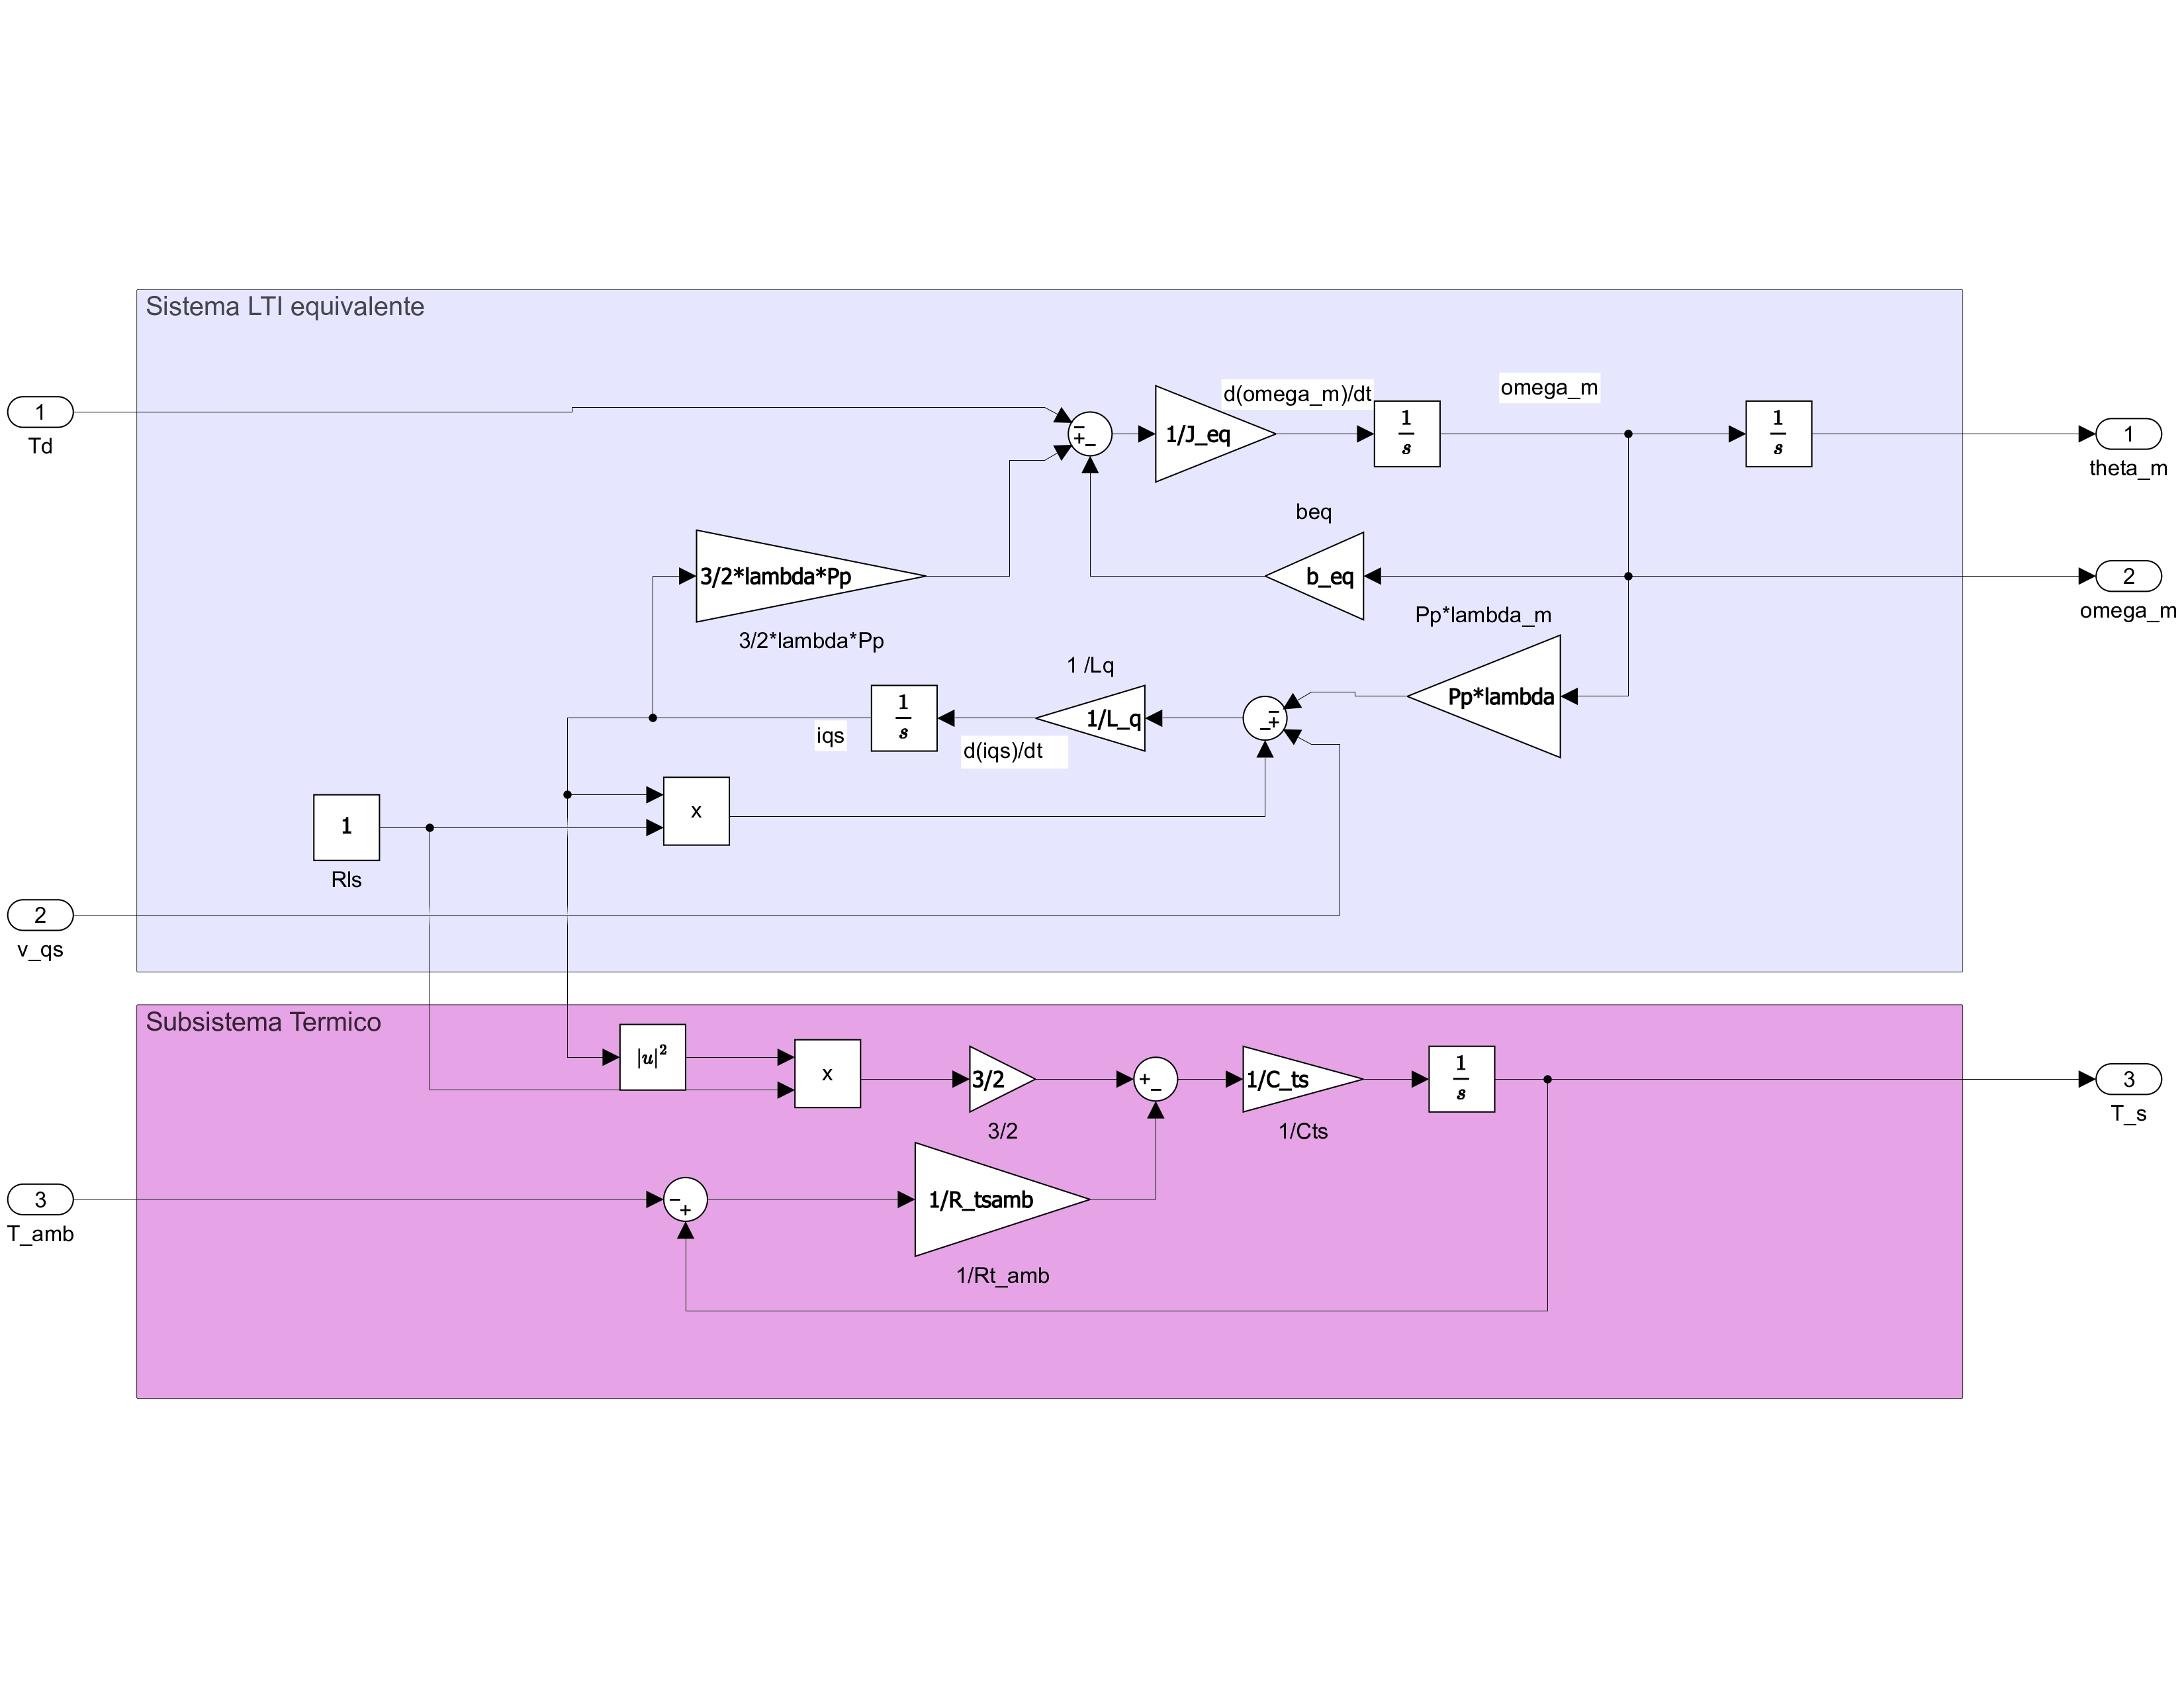
\includegraphics[width=\linewidth,height=0.36\textheight,keepaspectratio]{attachments/ltiequivalente.jpg}
    \caption{Diagrama de bloques del sistema LTI y subsistema térmico equivalente.}
    \label{fig:ltiequivalente}
\end{figure}
        

El modelo LTI equivalente se amplía incorporando la corriente
del eje directo $i_{ds}^{r}(t)$ como estado, lo que permite
considerar el caso $i_{ds}^{r}(0)\neq 0$. La Ley de Control
Mínima Complementaria \eqref{eq:ley-complementaria} cancela el
acoplamiento de esta corriente en la ecuación eléctrica del
eje en cuadratura. Para conservar una dinámica electromecánica
lineal, se desprecia el torque de reluctancia en el balance
mecánico. Con esta aproximación, el torque electromagnético
depende únicamente de la corriente de cuadratura.

\begin{equation}
\label{eq:modelo-lti-aumentado}
\begin{aligned}
& \left\{
    \begin{aligned}
        \frac{d\theta_m(t)}{dt} &= \omega_m(t) \\[1.5ex]
        \frac{d\omega_{m}(t)}{dt} &= \frac{1}{J_{eq}} \Bigg[ \frac{3}{2}P_{p} \lambda_{m}^{'r} i_{qs}^{r}(t) - b_{eq}  \omega_{m}(t) - \frac{T_d(t)}{r} \Bigg]  \\[1.5ex]
        \frac{di_{qs}^{r}(t)}{dt}  &= \frac{1}{L_{q} } \left[ v_{qs}^{r}(t) - R_{s}^{\ell} i_{qs}^{r}(t) - \lambda_{m}^{'r}P_{p} \omega_{m}(t) \right] \\[1.5ex]
        \frac{di_{ds}^{r}(t)}{dt} &= -\frac{1}{L_{d}} R_{s}^{\ell} i_{ds}^{r}(t)
    \end{aligned}
\right. \\[2ex]
& \frac{dT_{s}^{\circ}(t)}{dt} = \frac{1}{C_{ts}} \Bigg[ \frac{3}{2} R_{s}^{\ell}\Big(i_{qs}^{2}(t) +i_{ds}^{2}(t)\Big)  - \frac{T_{s}^{\circ}(t) - T_{amb}^{\circ}(t)}{R_{ts-amb}} \Bigg]
\end{aligned}
\end{equation}

Luego expresando de forma matricial de la forma $\dot{x}(t) = Ax(t) + B_u u(t) + B_d d(t)$ queda:
\begin{equation}
\label{eq:modelo-lti-aumentado-matricial}
\begin{bmatrix}
\frac{d\theta_m(t)}{dt} \\
\frac{d\omega_m(t)}{dt}  \\
\frac{d i^r_{qs}(t)}{dt} \\
\frac{d i^r_{ds}(t)}{dt}
\end{bmatrix}
=\begin{bmatrix}
0 & 1 & 0 & 0 \\
0 & \frac{-b_{eq}}{J_{eq}} & \frac{3}{2}\frac{P_p\lambda_{m} ^{'r}}{J_{eq}} & 0 \\
0 & -\frac{\lambda^{'r}_{m}P_p}{L_q} & -\frac{R^\ell_s}{L_q} & 0 \\
0 & 0 & 0 & -\frac{R_s^\ell}{Ld}
\end{bmatrix}
\begin{bmatrix}
\theta_m(t) \\
\omega_m(t) \\
i_{qs}^r(t) \\
i_{ds}^r(t)
\end{bmatrix}+\begin{bmatrix}
0 \\
0\\
\frac{1}{L_q}\\
0
\end{bmatrix}
v^r_{qs}+\begin{bmatrix}
0 \\
-\frac{1}{J_{eq}r}\\
0 \\
0
\end{bmatrix} 
T_d
\end{equation}

\begin{figure}[!htbp]
    \centering
    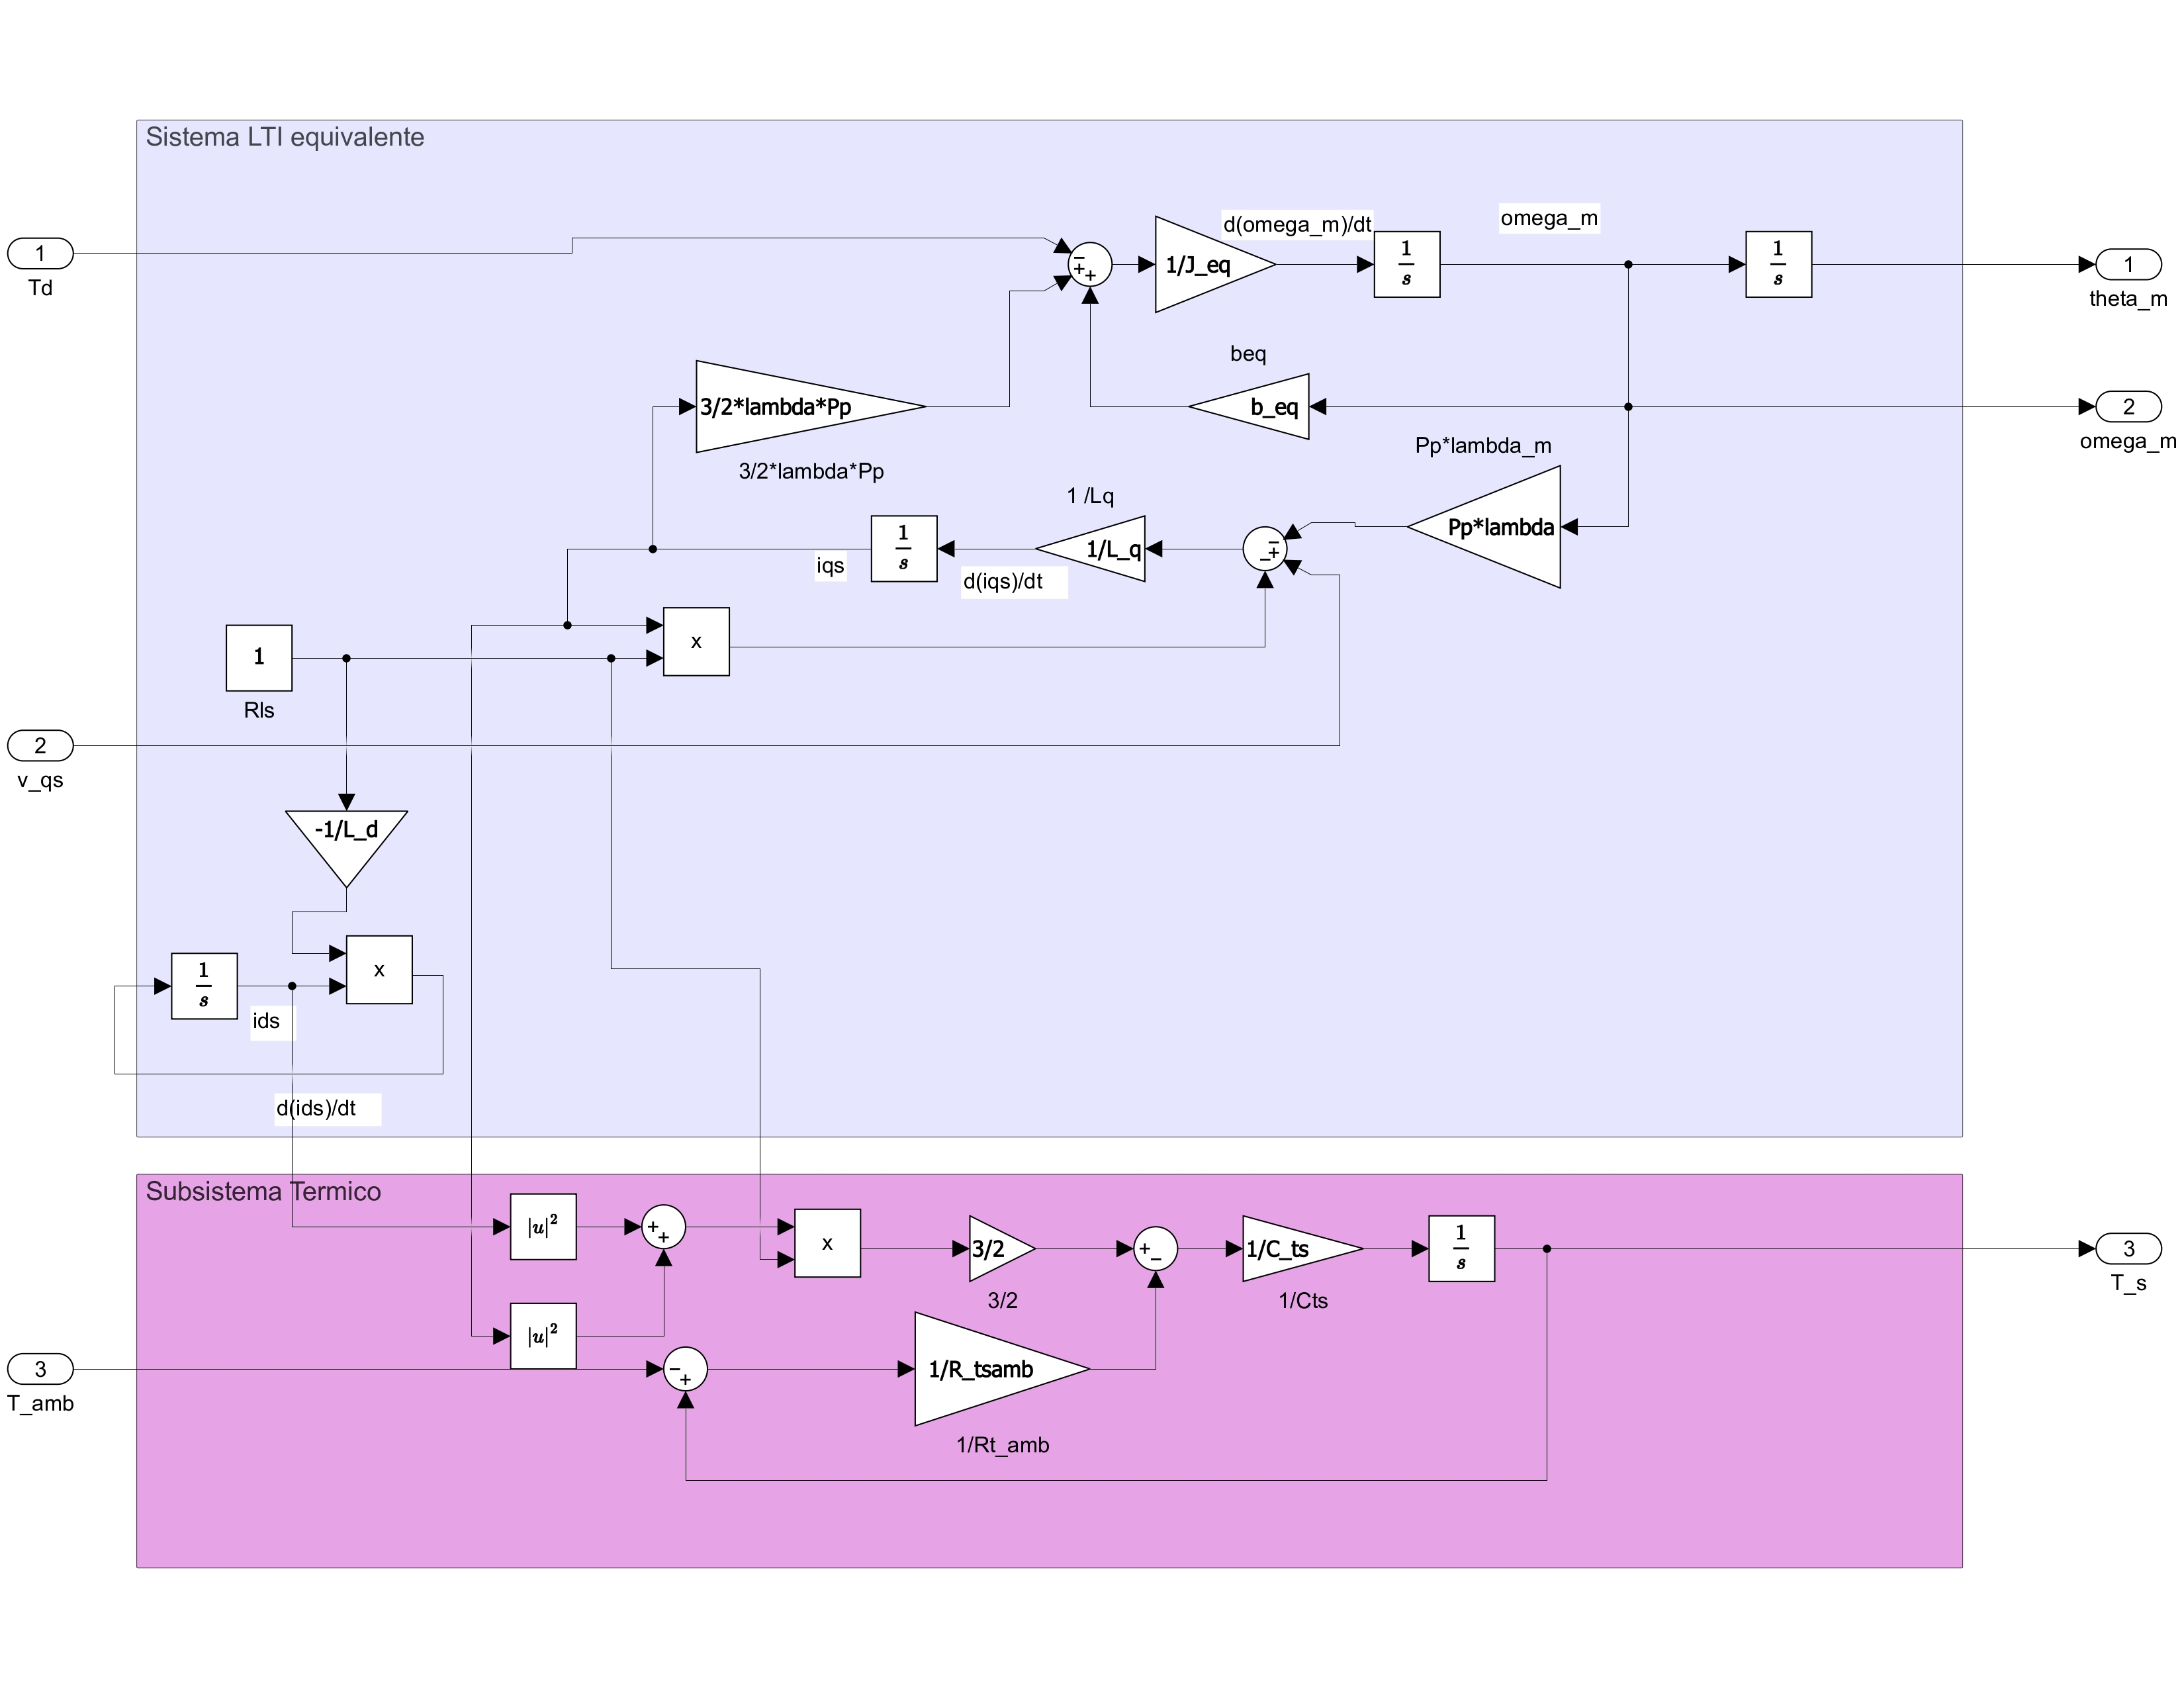
\includegraphics[width=\linewidth,height=0.43\textheight,keepaspectratio]{attachments/ltiaumentado.jpg}
    \caption{Diagrama de bloques del sistema LTI equivalente aumentado y subsistema térmico equivalente.}
    \label{fig:ltiaumentado}
\end{figure}





% ---------------------------------------------------------------------------- %
\subsubsection{Comparación del Modelo Dinámico LTI Equivalente Aumentado vs. el Modelo Dinámico Global LPV}
La evaluación de las estructuras modeladas expone un compromiso directo entre la simplicidad analítica y la precisión representativa. 

El modelo global LPV abarca el comportamiento general de la planta mediante la inclusión de los fenómenos térmicos sobre $R_s(T_s^\circ(t))$ y los términos de acoplamiento no lineal que vinculan las variables mecánicas y eléctricas; esta flexibilidad en la formulación permite la representación matemática del sistema y abre el espectro operacional hacia zonas de trabajo multifuncionales (regímenes de reforzamiento y debilitamiento de campo).  

En sentido inverso, la implementación del modelo LTI Equivalente Aumentado recurre a la restricción operativa de imponer $i^r_{ds} \equiv 0$, extinguiendo la influencia de la corriente directa sobre la dinámica electromecánica global. Si bien este procedimiento linealiza e independiza los canales de control (simplificando la estructura matricial de estado del sistema), reduce el rango operativo local a las proximidades de la condición cuasi-estacionaria de diseño. Consecuentemente, el modelo LTI disminuye su fidelidad ante variaciones dinámicas rápidas fuera de dicho entorno, pero ratifica su aptitud analítica para predecir con solvencia el estado estacionario y las tendencias macroscópicas del sistema bajo estudio. 

\subsubsection{Efectos de la Corriente de Eje Directo: Debilitamiento y Reforzamiento de Campo}
Se evaluará el comportamiento del modelo LPV para otros puntos de operación tales como: 

\begin{itemize}
    \item $i_{ds}^r>0$ (reforzamiento de campo)
    \item $i_{ds}^r<0$ (debilitamiento del campo)
\end{itemize}

Al analizar el sistema, se concluye que estos cambios se ven reflejados principalmente en la ecuación del torque electromagnetico \eqref{SubElec3} y la ecuación de la variación de la corriente del eje en cuadratura \eqref{variacion_ids}
\[
\left\{
\begin{aligned}
 T_{m}(t)  &  = \frac{3}{2}P_{p} \lambda_{m}^{'r} i_{qs}^{r}(t) + \frac{3}{2} P_{p} \Big( L_{d} - L_{q} \Big) i_{qs}^{r}(t) i_{ds}^{r}(t) \\
 \frac{di_{ds}^{r}(t)}{dt}  & = \frac{1}{L_{d}} \left[ v_{ds}^{r}(t) - R_{s} \Big( T_{s}^{\circ} (t) \Big) i_{ds}^{r}(t) + L_{q}i_{qs}^{r}(t) \omega_{m}(t)P_{p}  \right] 
\end{aligned}
\right.
\]


Luego, considerando un estado estacionario $\Big(\frac{di_{ds}^r}{dt}=0 \Big)$ es posible despejar la velocidad angular del motor $\omega_m$, lo que nos permite obtener la expresión:

\begin{equation}
\label{eq:velocidad-equilibrio}
\omega_{m}(t) = \frac{R_{s} \Big( T_{s}^{\circ} (t) \Big) i_{ds}^{r}(t) - v_{ds}^{r}(t)}{P_{p} L_{q} i_{qs}^{r}(t)}
\end{equation}

Analizando la ecuación de torque electromagnético y la ecuación de velocidad angular del motor para cada caso (teniendo en cuenta que es una máquina de polos salientes donde $L_d>L_q$), se pueden estudiar 2 situaciones:
\begin{itemize}
    \item Caso $i^r_{ds}>0$ (Reforzamiento de campo):
    
    Dado que $L_d > L_q$, el término de reluctancia $(L_d - L_q)i_{ds}^r$ incrementa el flujo magnético efectivo en la ecuación del torque. Como consecuencia, el par motor disponible $T_m$ se refuerza (aumenta) a bajas velocidades. En contraparte, al evaluar la velocidad angular en régimen estacionario, los términos en el numerador de su expresión matemática se oponen, provocando que la velocidad de equilibrio disminuya bajo una potencia aproximadamente constante.
    \[
    i_{ds}^{r} > 0 \implies \left\{ 
    \begin{aligned}
    T_{m} &\uparrow \quad \text{(se refuerza)} \\
    \omega_{m} &\downarrow \quad \text{(se reduce)}
    \end{aligned}
    \right.
    \]

    \item Caso $i^r_{ds}<0$ (Debilitamiento de campo):
    
    En este escenario, el término $(L_d - L_q)i_{ds}^r$ se vuelve negativo, reduciendo el flujo efectivo, lo que se traduce en una disminución del torque electromagnético desarrollado $T_m$. Por otra parte, analizando la velocidad angular de rotación, el término óhmico $R_s i_{ds}^r$ en el numerador adopta un signo negativo que se acopla con la tensión de control. Esto reduce la contratensión requerida, permitiendo un incremento significativo de la velocidad de equilibrio de la máquina sin sobrepasar el límite de tensión impuesto por el inversor.   
    \[
    i_{ds}^{r} < 0 \implies \left\{ 
    \begin{aligned}
    T_{m} &\downarrow \quad \text{(se reduce)} \\
    \omega_{m} &\uparrow \quad \text{(se refuerza)}
    \end{aligned}
    \right.
    \]
\end{itemize}

\subsubsection{Funciones de Transferencia}

Para obtener las funciones de transferencia del modelo LTI
equivalente aumentado, se parte del sistema \eqref{eq:modelo-lti-transferencias}.
Se toma la tensión del eje en cuadratura $v_{qs}^{r}$ como entrada de
control, el torque $T_d$ como entrada de perturbación y la posición
angular del motor $\theta_m$ como salida. 

\begin{equation}
\label{eq:modelo-lti-transferencias}
\left\{
\begin{aligned}
\frac{d\theta_m(t)}{dt} &= \omega_m(t) \\[1.5ex]
\frac{d\omega_{m}(t)}{dt} &= \frac{1}{J_{eq}} \Bigg[ \frac{3}{2}P_{p} \lambda_{m}^{'r} i_{qs}^{r}(t) - b_{eq} \omega_{m}(t) - \frac{T_d(t)}{r} \Bigg]  \\[1.5ex]
\frac{di_{qs}^{r}(t)}{dt}  &= \frac{1}{L_{q} } \left[ v_{qs}^{r}(t) - R_{s}^{\ell} i_{qs}^{r}(t) - \lambda_{m}^{'r}P_{p} \omega_{m}(t) \right]
\end{aligned}
\right.
\end{equation}

A continuación, se realiza el estudio de la dinámica del modelo LTI Equivalente Aumentado en el plano complejo $s$; para ello, se aplica la transformada de Laplace $\mathcal{L}\{\;\}$ a todas las ecuaciones, dejando así:

\begin{equation*}
\left\{
\begin{aligned}
s\Theta_m(s) &= \Omega_m(s)\\
s\Omega_m(s) &= \frac{1}{J_{eq}}\Big(\frac{3}{2}P_p\lambda^{'r}_mI^r_{qs}(s)-b_{eq}\Omega_m(s)-\frac{T_d(s)}{r}\Big)\\
sI^r_{qs}(s) &= \frac{1}{L_q}\Big(V^r_{qs}(s)-R^\ell_{s}I^r_{qs}(s)-\lambda^{'r}_mP_p\Omega_m(s)\Big)
\end{aligned}
\right.
\end{equation*}
Trabajando matemáticamente llegamos a la siguiente igualdad:
\begin{equation}
\label{eq:respuesta-posicion-la}
    \Theta_m(s) = \frac{3P_p\lambda_m^{'r}V_{qs}^r(s)-2\Big(L_qs+R^\ell_s\Big)\frac{T_d(s)}{r}}{2J_{eq}L_qs^3+2\Big(J_{eq}R_s^\ell+b_{eq}L_q\Big)s^2+\Big(2b_{eq}R_s^\ell+3\Big(P_p\lambda^{'r}_m\Big)^2\Big)s}
\end{equation}
Por lo tanto, las funciones de transferencia para las entradas $V^r_{qs}(s)$ y $T_d(s)$:
\begin{equation}
\label{eq:transferencia-tension-la}
    G_{V^r_{qs}}(s)=\frac{\Theta_m(s)}{V_{qs}^r(s)} = \frac{3P_p\lambda_m^{'r}}{2J_{eq}L_qs^3+2\Big(J_{eq}R_s^\ell+b_{eq}L_q\Big)s^2+\Big(2b_{eq}R_s^\ell+3\Big(P_p\lambda^{'r}_m\Big)^2\Big)s}    
\end{equation}
\begin{equation}
\label{eq:transferencia-carga-la}
    G_{T_d}(s)=\frac{\Theta_m(s)}{T_d(s)}= \frac{-2\Big(L_qs+R^\ell_s\Big)\frac{1}{r}}{2J_{eq}L_qs^3+2\Big(J_{eq}R_s^\ell+b_{eq}L_q\Big)s^2+\Big(2b_{eq}R_s^\ell+3\Big(P_p\lambda^{'r}_m\Big)^2\Big)s}
\end{equation}
Ed ésta manera podemos expresar al sistema tal que: 
\begin{equation}
\label{eq:superposicion-la}
    \Theta_m(s)=G_{V^r_{qs}}(s)V^r_{qs}(s)+G_{T_d}(s)T_d(s)
\end{equation}
% ---------------------------------------------------------------------------- %
\subsection{Análisis de Estabilidad a lazo abierto para el modelo LTI equivalente aumentado}

El análisis a lazo abierto parte de las funciones de transferencia
\eqref{eq:transferencia-tension-la} y \eqref{eq:transferencia-carga-la}r. Las raíces de su denominador común \eqref{eq:polinomio-la} son los polos de ambos
canales. Esto deja como polinomio característico la siguiente expresión:

\begin{equation}
\label{eq:polinomio-la}
P(s) = 2J_{eq}L_qs^3+2\Big(J_{eq}R_s^\ell+b_{eq}L_q\Big)s^2+\Big(2b_{eq}R_s^\ell+3\Big(P_p\lambda^{'r}_m\Big)^2\Big)s
\end{equation}
Para obtener los polos del sistema LTI Equivalente Aumentado se iguala el polinomio característico a cero y se evalúan las raíces del polinomio:
\begin{equation*}
P(s) = 2J_{eq}L_qs^3+2\Big(J_{eq}R_s^\ell+b_{eq}L_q\Big)s^2+\Big(2b_{eq}R_s^\ell+3\Big(P_p\lambda^{'r}_m\Big)^2\Big)s=0
\end{equation*}

como es posible aplicarse factor común $s$, se concluye que uno de los polos se encuantra en $s_1=0$. Ël resto de la expresión deja un polinomio de segundo orden, lo que implica 2 raíces adicionales, que tendrán los valores según la formula resolvente de raices cuadráticas: 

\begin{equation}
\label{eq:polos-la}
    \begin{cases} 
        s_1 = 0 \\ 
        s_{2,3} = \frac{-2\left(J_{eq}R_s^\ell+b_{eq}L_q\right) \pm \sqrt{4\left(J_{eq}R_s^\ell+b_{eq}L_q\right)^2 - 8J_{eq}L_q\left(2b_{eq}R_s^\ell+3\left(P_p\lambda^{'r}_m\right)^2\right)}}{4J_{eq}L_q} 
    \end{cases}
\end{equation}

La función de transferencia de la tensión del eje en cuadratura
a la posición angular del motor \eqref{eq:transferencia-tension-la}
tiene un numerador constante distinto de cero. El único cero
de los dos canales corresponde a la función de transferencia del
torque de perturbación $T_d$ a la posición angular $\theta_m$
\eqref{eq:transferencia-carga-la}. Para calcularlo, se iguala a cero
el factor del numerador que depende de $s$:

\begin{equation*}
    L_qs+R^\ell_s=0
\end{equation*}

que despejando, permite apreciar el cero en 

\begin{equation}
\label{eq:cero-carga-la}
    s=-\frac{R^\ell_s}{L_q}
\end{equation}

Luego, reemplazando los valores de las variables, variando el valor de temperatura y optando por un valor de resistencia lineal $R_s^\ell$ afin a la temperatura estudiada, se puede armar la tabla \ref{tab:polosyceros}.

\begin{table}[htbp]
    \centering
\caption{Resistencia, Polos y Ceros del sistema variando la Temperatura con $J_{eq}=19,78 \cdot 10^{-6}$ (mínimo).}
\label{tab:polosyceros}
\begin{tabular}{lllll}
\hline
$T^\circ_s(\circ C) $&$ R^\ell_s $&$ p_1 $&$ p_2 $&$ z $\\
\hline
 $ 20$&$1,0200 $  & $-88,49+149,97 i$     & $  -88,49-149,97 i$    &$ -175.8621 $ \\
 $ 40$&$ 1,0996  $ &$ -95,34+145,75 i$     & $-95,34- 145,75 i$     & $-189.5793  $\\
  $60$&$ 1,1791$  & $-102,20+141,08 i $    &$-102,20-141,08 i $     &$-203.2966 $\\
  $  80$&$1,2587$   &$ -109,06+135,91 i $    &$-109,06-135,91 i $     & $-217.0138  $\\
    $100$& $1,3382$  & $-115,92+130,17 i $    &$-115,92-130,17 i$      &$ -230.7310$  \\
   $ 120$&$ 1,4178$  &$ -122,78+123,78 i$     &$-122,78-123,78 i$      & $-244.4483  $\\
   $ 140$&$ 1,4974  $&$-129,64+116,64 i $     &$-129,64-116,64 i $     &$ -258.1655  $\\
\hline
\end{tabular}
\end{table}

\begin{figure}[!htbp]
    \centering
    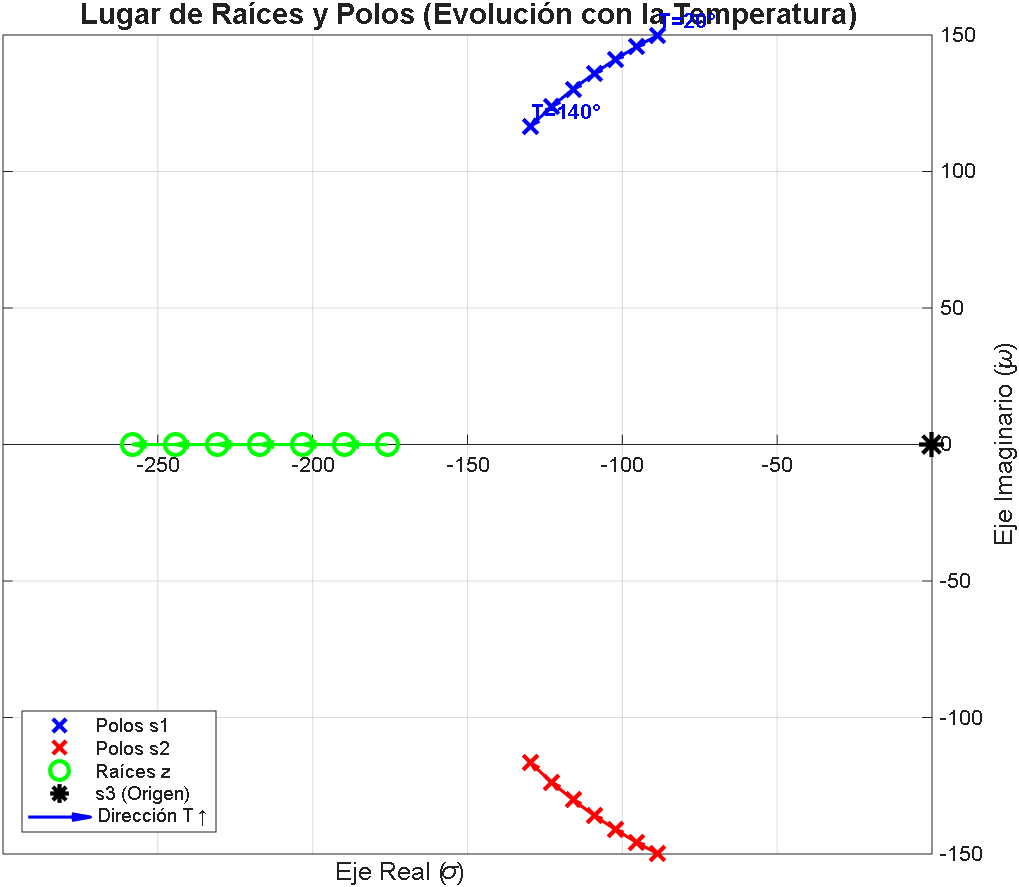
\includegraphics[width=0.66\linewidth,height=0.34\textheight,keepaspectratio]{attachments/polosyceros.png}
    \caption{Polos y Ceros del sistema variando la Temperatura con $J_{eq}=19,78*10^{-6}$ (mínimo)}
    \label{fig:polos-ceros-temperatura}
\end{figure}

Al realizar el análisis, se aprecia que tanto los polos como los ceros del sistema se encuentran en el semiplano con parte real negativa del plano complejo: con esto se concluye la existencia de estabilidad en el sistema. También se puede apreciar que al aumentar la temperatura (lo cual implica aumento de la resistencia linealizada) los polos se mantiene en el mismo semiplano del plano complejo. 

% ---------------------------------------------------------------------------- %
\subsection{Análisis de Observabilidad completa de estado para el modelo LTI equivalente aumentado}
Para evaluar la observabilidad completa de estado del modelo LTI Equivalente Aumentado (considerando la Ley de Control Mínima Complementaria, valor inicial  $i_{ds}^{r}(t) \equiv 0$ y despreciando el efecto de la temperatura $T_{s}^{o}(t)$) desde la variable de salida $\theta_m(t)$, se emplea el criterio de Kalman. Este criterio establece que un sistema LTI de orden $n$ es completamente observable si el rango de la matriz de observabilidad $\mathcal{O}$ es igual a $n$. En consecuencia, dado que $\mathcal{O}$ es una matriz cuadrada, el sistema será observable si su determinante es distinto de cero ($\det(\mathcal{O}) \neq 0$).

La matriz de observabilidad $\mathcal{O}$ queda definida tal que:
\begin{equation}
\label{eq:observabilidad-kalman}
\mathcal{O} = \begin{bmatrix}
C \\
CA \\
CA^2 \\
\vdots \\
CA^{n-1}
\end{bmatrix}
\end{equation}

Donde: 

\[
A = \begin{bmatrix}
0 & 1 & 0 \\
0 & \frac{-b_{eq}}{J_{eq}} & \frac{3}{2}\frac{P_p\lambda_{m}^{'r}}{J_{eq}} \\
0 & -\frac{\lambda^{'r}_{m}P_p}{L_q} & -\frac{R^\ell_s}{L_q}
\end{bmatrix}
\qquad
C_\theta=\begin{bmatrix}
    1& 0& 0
\end{bmatrix}
\]

Entonces, la matriz de observabilidad teniendo como salida únicamente $\theta_m$ queda:

\begin{equation}
\label{eq:observabilidad-posicion}
    \mathcal{O}_{\theta_m} = \begin{bmatrix}
C_\theta \\
C_\theta A \\
C_\theta A^2
\end{bmatrix}=\begin{bmatrix}
1 & 0 & 0 \\
0 & 1 & 0 \\
0 & -\frac{b_{eq}}{J_{eq}} & \frac{3}{2}\frac{P_p\lambda_{m}^{'r}}{J_{eq}}
\end{bmatrix}
\end{equation}

El determinante de la matriz de observabilidad
\eqref{eq:observabilidad-posicion} es
\[
    \det(\mathcal{O}_{\theta_m})
    = \frac{3P_p\lambda_m^{'r}}{2J_{eq}}
    \neq 0.
\]
Por lo tanto, $\mathcal{O}_{\theta_m}$ tiene rango tres.
Según el criterio de Kalman, los tres estados del modelo LTI
reducido, $\theta_m$, $\omega_m$ e $i_{qs}^{r}$, son observables
a partir de la medición de la posición angular del motor
$\theta_m$.

Si ahora se evalúa la observabilidad de la salida $\omega_m$, donde $C$ pasa a valer 

\[
C_\omega =\begin{bmatrix} 0&1&0 \end{bmatrix}
\]

entonces, la matriz de observabilidad queda tal que:

\begin{equation}
\label{eq:observabilidad-velocidad}
    \mathcal{O}_{\omega_m} = \begin{bmatrix}
0 & 1 & 0 \\
0 & -\frac{b_{eq}}{J_{eq}} & \frac{3}{2}\frac{P_p\lambda_{m}^{'r}}{J_{eq}} \\
0 & \left( \frac{b_{eq}^2}{J_{eq}^2} - \frac{3}{2}\frac{P_p^2 (\lambda_{m}^{'r})^2}{J_{eq}L_q} \right) & -\frac{3}{2}\frac{P_p\lambda_{m}^{'r}}{J_{eq}} \left( \frac{b_{eq}}{J_{eq}} + \frac{R^\ell_s}{L_q} \right)
\end{bmatrix}
\end{equation}

y al evaluar el determinante de la matriz (que a simple vista puede deducirse nulo, debido a la primer columna siendo nula)

\[
det(\mathcal{O_{\omega_m}})=0
\]

La matriz de observabilidad $\mathcal{O}_{\omega_m}$ tiene rango dos.
Por el criterio de Kalman, el modelo LTI reducido de tres estados
es parcialmente observable a partir de la velocidad angular
$\omega_m$. En particular, la posición inicial del motor queda
indeterminada. La integración de la señal del tacogenerador
permite calcular el desplazamiento angular, pero para determinar
la posición absoluta de la carga se requiere conocer la posición
inicial o disponer de una referencia angular adicional.

% ---------------------------------------------------------------------------- %
\subsection{Análisis de Controlabilidad completa de estado para el modelo LTI Equivalente Aumentado}

Nuevamente con el criterio de Kalman se analizará la controlabilidad completa del sistema LTI Equivalente Aumentado (considerando la Ley de Control Mínima Complementaria, valor inicial  $i_{ds}^{r}(t) \equiv 0$ y despreciando el efecto de la temperatura $T_{s}^{o}(t)$) desde la entrada manipulada $v_{qs}^r(t)$ y sin considerar la perturbación de la carga mecánica, es decir, teniendo en cuanta solo $B_u$ sin $B_w$. 

Para calcular la matriz de controlabilidad del sistema, se calcula:

\begin{equation}
\label{eq:controlabilidad-kalman}
    C = \begin{bmatrix} B & AB & \cdots & A^{n-1}B \end{bmatrix}
\end{equation}
Donde:
\[
A = \begin{bmatrix}
0 & 1 & 0 \\
0 & \frac{-b_{eq}}{J_{eq}} & \frac{3}{2}\frac{P_p\lambda_{m}^{'r}}{J_{eq}} \\
0 & -\frac{\lambda^{'r}_{m}P_p}{L_q} & -\frac{R^\ell_s}{L_q}
\end{bmatrix}
\qquad
B_u = \begin{bmatrix}
0 \\
 0\\
 \frac{1}{L_q}
\end{bmatrix}
\]

Con esto la matriz de Controlabilidad es la siguiente: 

\begin{equation}
\label{eq:controlabilidad-lti}
C = \begin{bmatrix} B_u & AB_u & A^2B_u \end{bmatrix} = \begin{bmatrix}
0 & 0 & \frac{3}{2}\frac{P_p \lambda_{m}^{'r}}{J_{eq} L_{q}} \\
0 & \frac{3}{2}\frac{P_p \lambda_{m}^{'r}}{J_{eq} L_{q}} & -\frac{3}{2}\frac{P_p \lambda_{m}^{'r} b_{eq}}{J_{eq}^2 L_{q}} - \frac{3}{2}\frac{P_p R^\ell_s \lambda_{m}^{'r}}{J_{eq} L_{q}^2} \\
\frac{1}{L_{q}} & -\frac{R^\ell_s}{L_{q}^2} & \frac{(R^\ell_s)^{2}}{L_{q}^3} - \frac{3}{2}\frac{P_p^{2} (\lambda_{m}^{'r})^{2}}{J_{eq} L_{q}^2}\end{bmatrix}
\end{equation}

Y su determinante: 
\[
det(C)=-\frac{9}{4} \frac{P_p^2 (\lambda_{m}^{'r})^2}{J_{eq}^2 L_q^3}\neq 0
\]

Como $\det(C)\neq 0$, la matriz de controlabilidad
\eqref{eq:controlabilidad-lti} tiene rango tres. Por el criterio
de Kalman, el modelo LTI reducido es completamente controlable
mediante la tensión del eje en cuadratura $v_{qs}^{r}(t)$.

Debido a que no tenemos control sobre la variable de entrada $T_d(t)$, no es de interes estudiar su controlabilidad.

% ---------------------------------------------------------------------------- %
\subsection{Simulación Dinámica en el Dominio del Tiempo, comparando el Modelo NL Completo Desacoplado con Ley de Control NL vs LTI Equivalente Aumentado}
Se analizara la respuesta del estado interno \{$\theta_m(t);\omega_m(t);i_{dq0s}(t);T^\circ_s(t)$\} ante consignas de tensión de amplitud ${v^r_{qs}}^*$ superpuesta con una perturbación $T_l$. Siendo las entradas las siguientes y considerando temperatura ambiente $T_{amb}=20^\circ C$, se tiene:


\begin{figure}[!htbp]
    \centering
    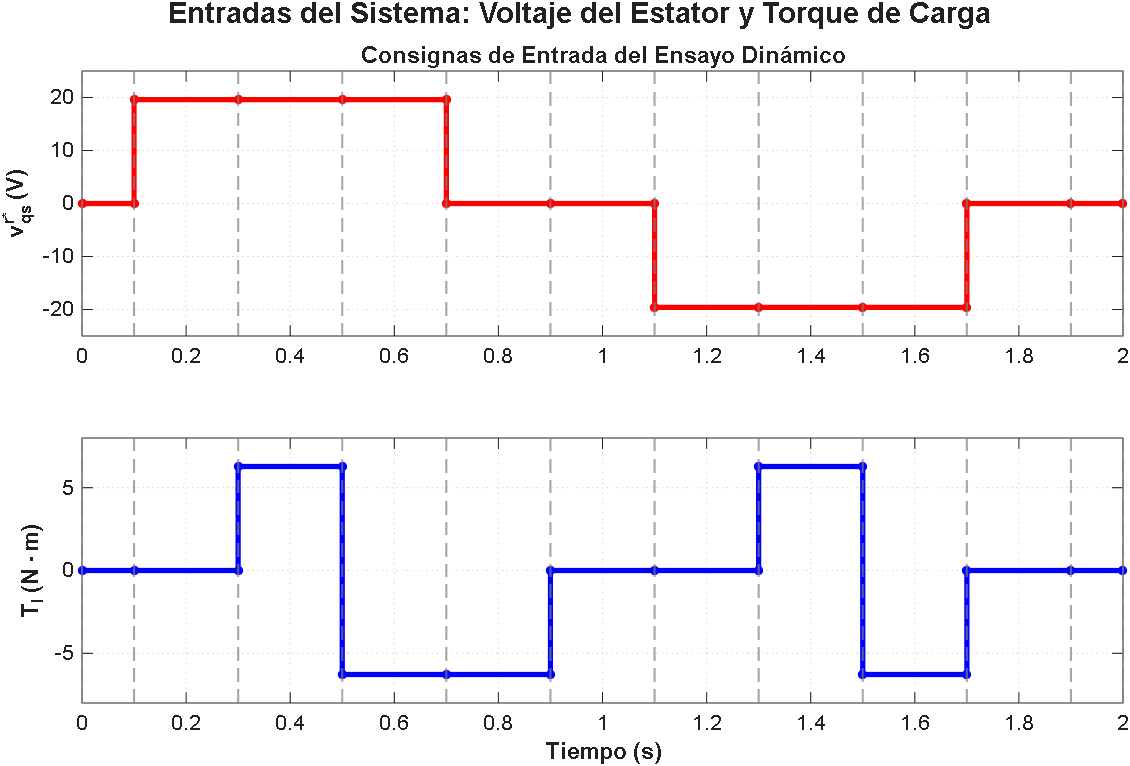
\includegraphics[width=0.75\linewidth,keepaspectratio]{attachments/VariacionTorqueyTension.png}
    \caption{Perfiles de entrada utilizados en el ensayo dinámico: tensión de referencia en el eje en cuadratura $v_{qs}^{*r}(t)$ (arriba) y torque de carga $T_l(t)$ (abajo).}
    \label{fig:entradas-simulacion}
\end{figure}
\subsubsection{Análisis de respuesta del estado interno}
Considerando como condiciones iniciales una $T_{amb}=20^\circ C$ y una corriente virtual de eje directo $i^r_{ds}(0)=0 \;A$, a continuación se presentan los gráficos obtenidos de: $\theta_m$, $\omega_m$, $i^r_d$, $i^r_q$,$i_a$,$i_b$, $i_c$, $T_s$ donde se mantiene que en amarillo vemos la curva del modelo LTI equivalente aumentado y en azul vemos el modelo no lineal desacoplado mediante realimentación.

\begin{figure}[!htbp]
    \centering
    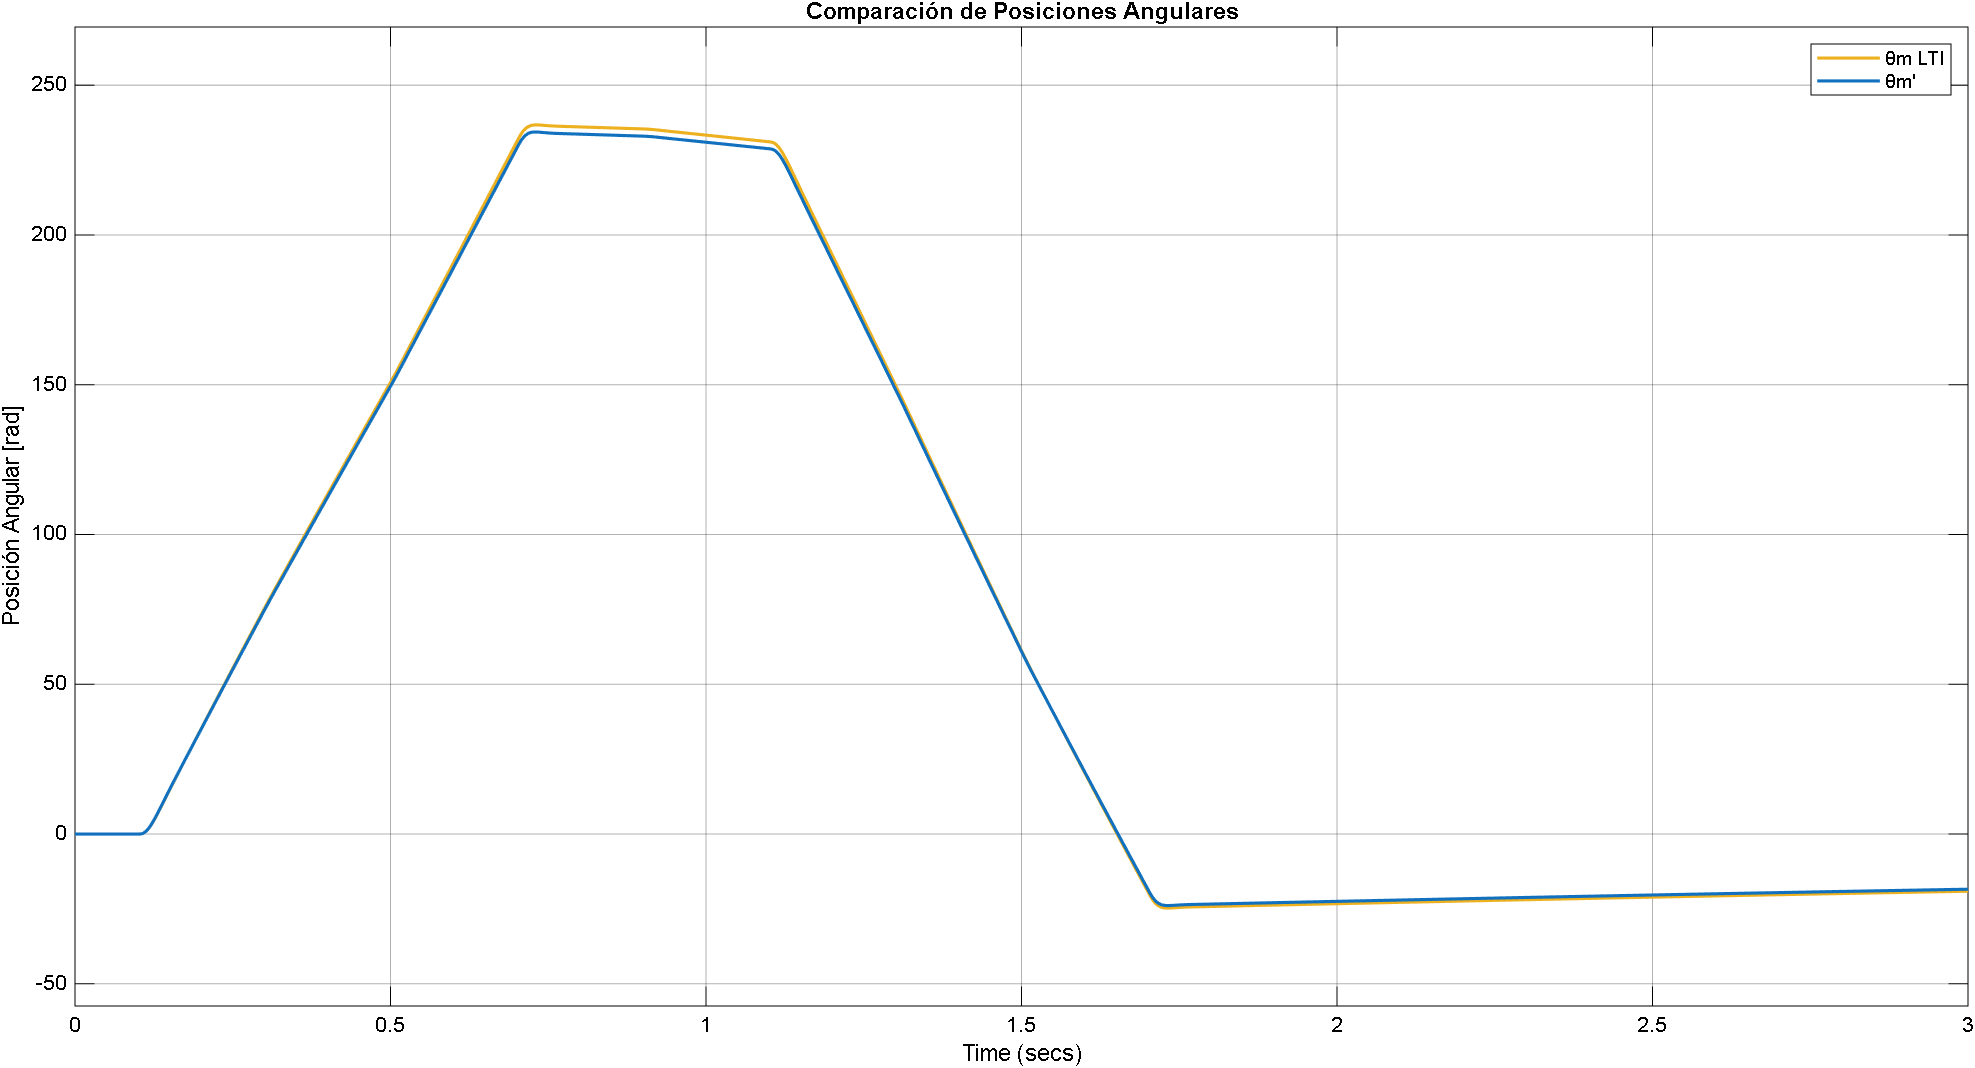
\includegraphics[width=0.86\linewidth,height=0.40\textheight,keepaspectratio]{attachments/Compa_NL_LTI_posici_ang.png}
    \caption{Evolución temporal de la posición angular del motor $\theta_m(t)$: comparación entre el modelo no lineal desacoplado mediante realimentación y el modelo LTI equivalente aumentado.}
    \label{fig:pcomparacion-posicion}
\end{figure}

\begin{figure}[!htbp]
    \centering
    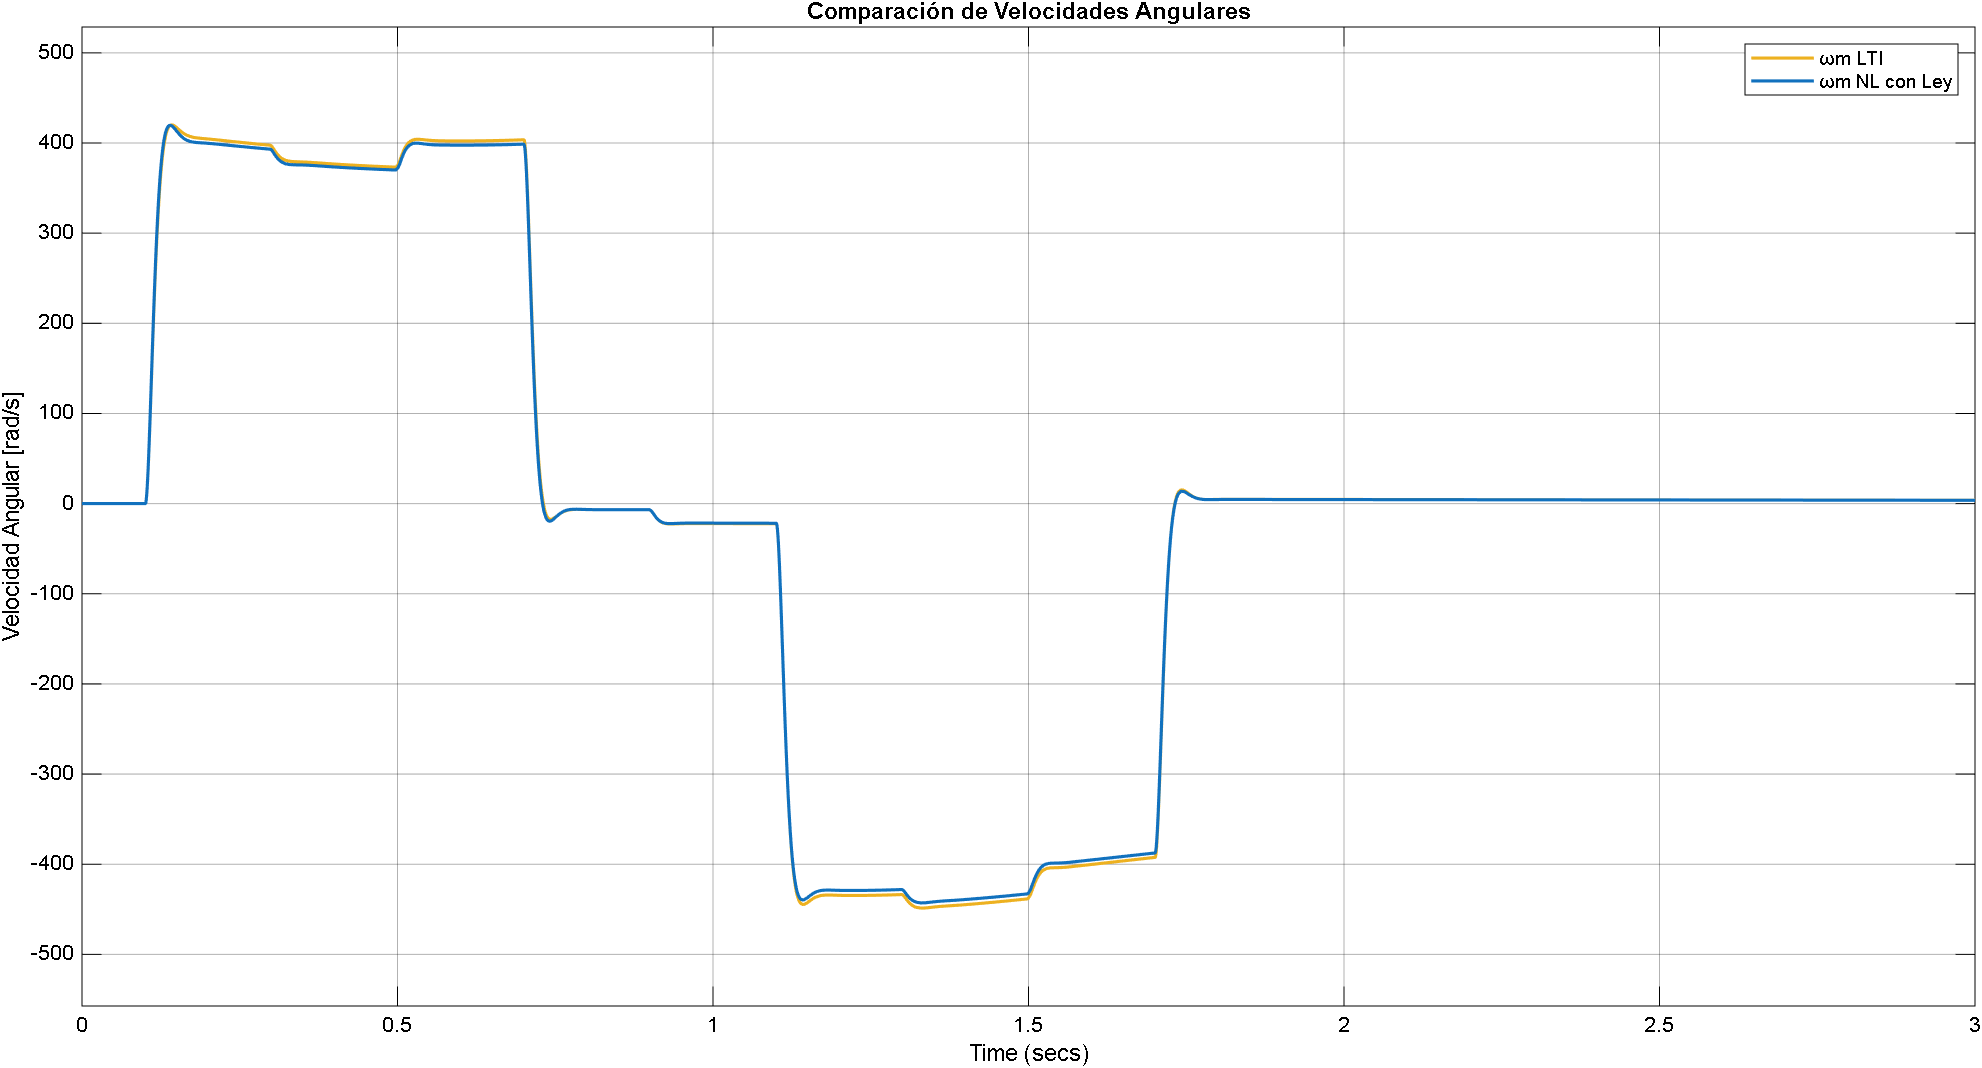
\includegraphics[width=0.86\linewidth,height=0.40\textheight,keepaspectratio]{attachments/Compa_NL_LTI_vel_ang.png}
    \caption{Evolución temporal de la velocidad angular del motor $\omega_m(t)$: comparación entre el modelo no lineal desacoplado mediante realimentación y el modelo LTI equivalente aumentado.}
    \label{fig:comparacion-velocidad}
\end{figure}


Observamos que la velocidad presenta pequeños sobrepicos transitorios ante los cambios bruscos de tensión y las perturbaciones de carga, mientras que el torque electromagnético.

\begin{figure}[!htbp]
    \centering
    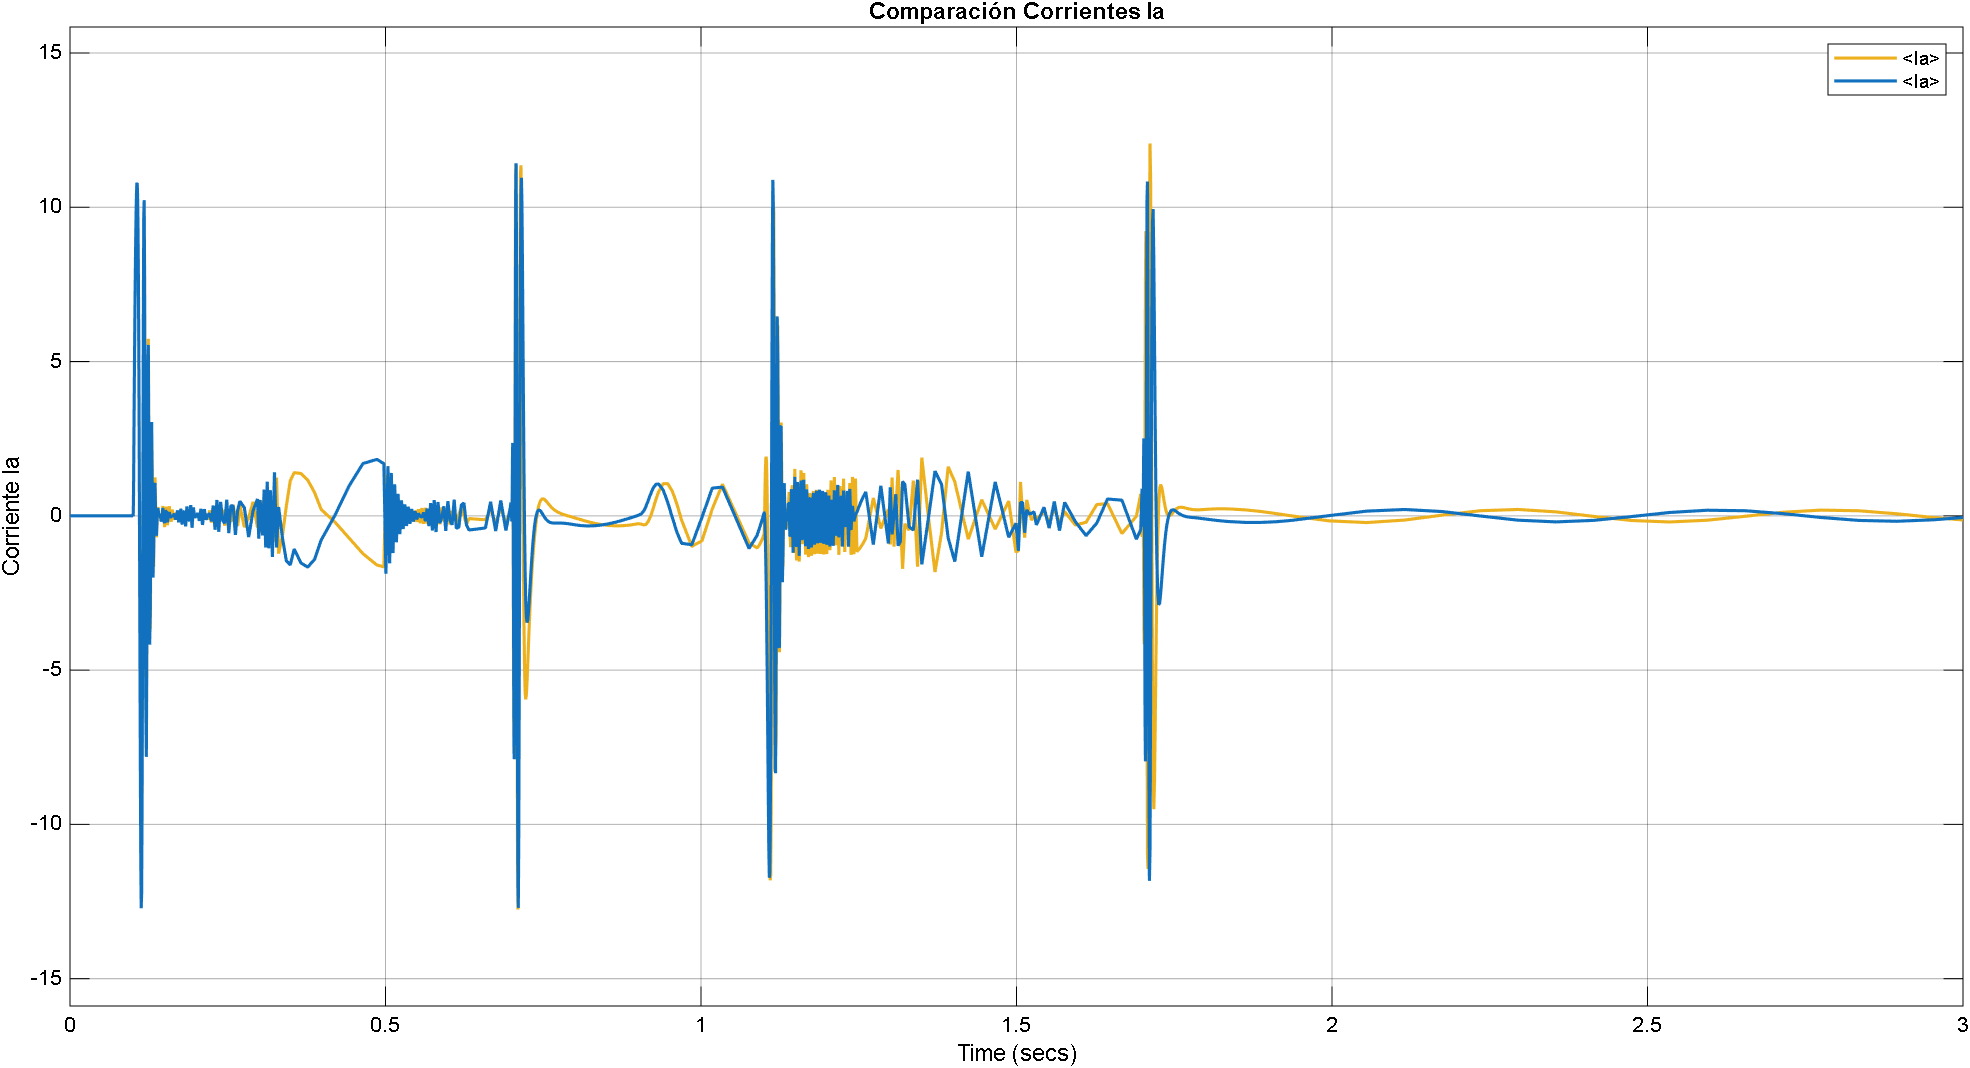
\includegraphics[width=0.86\linewidth,height=0.40\textheight,keepaspectratio]{attachments/Compa_NL_LTI_Ia.png}
    \caption{Evolución temporal de la corriente de fase $i_{as}(t)$. Se comparan el modelo LTI equivalente aumentado (trazo amarillo) y el modelo no lineal desacoplado mediante realimentación (trazo azul).}
    \label{fig:comparacion-corriente-a}
\end{figure}

\begin{figure}[!htbp]
    \centering
    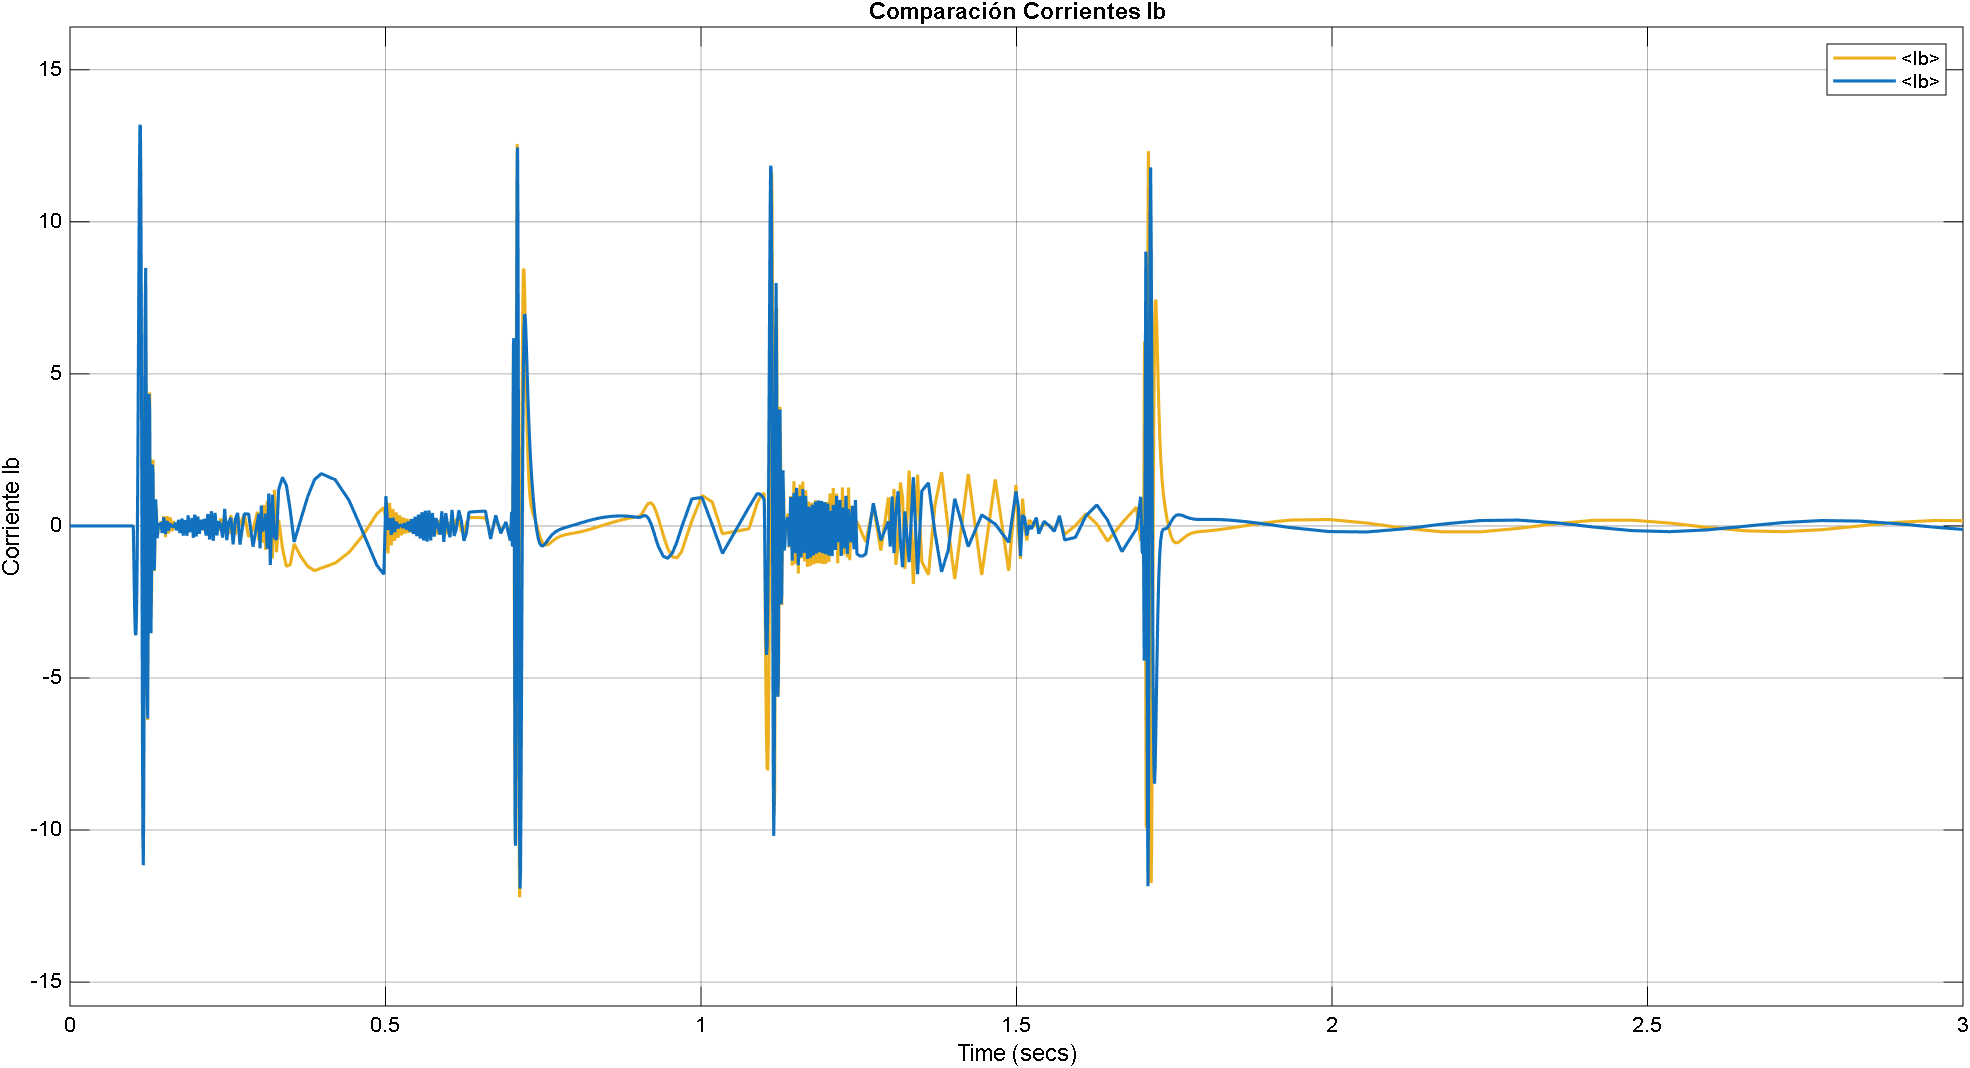
\includegraphics[width=0.86\linewidth,height=0.40\textheight,keepaspectratio]{attachments/Compa_NL_LTI_Ib.png}
    \caption{Evolución temporal de la corriente de fase $i_{bs}(t)$. Se comparan el modelo LTI equivalente aumentado (trazo amarillo) y el modelo no lineal desacoplado mediante realimentación (trazo azul).}
    \label{fig:comparacion-corriente-b}
\end{figure}

\begin{figure}[!htbp]
    \centering
    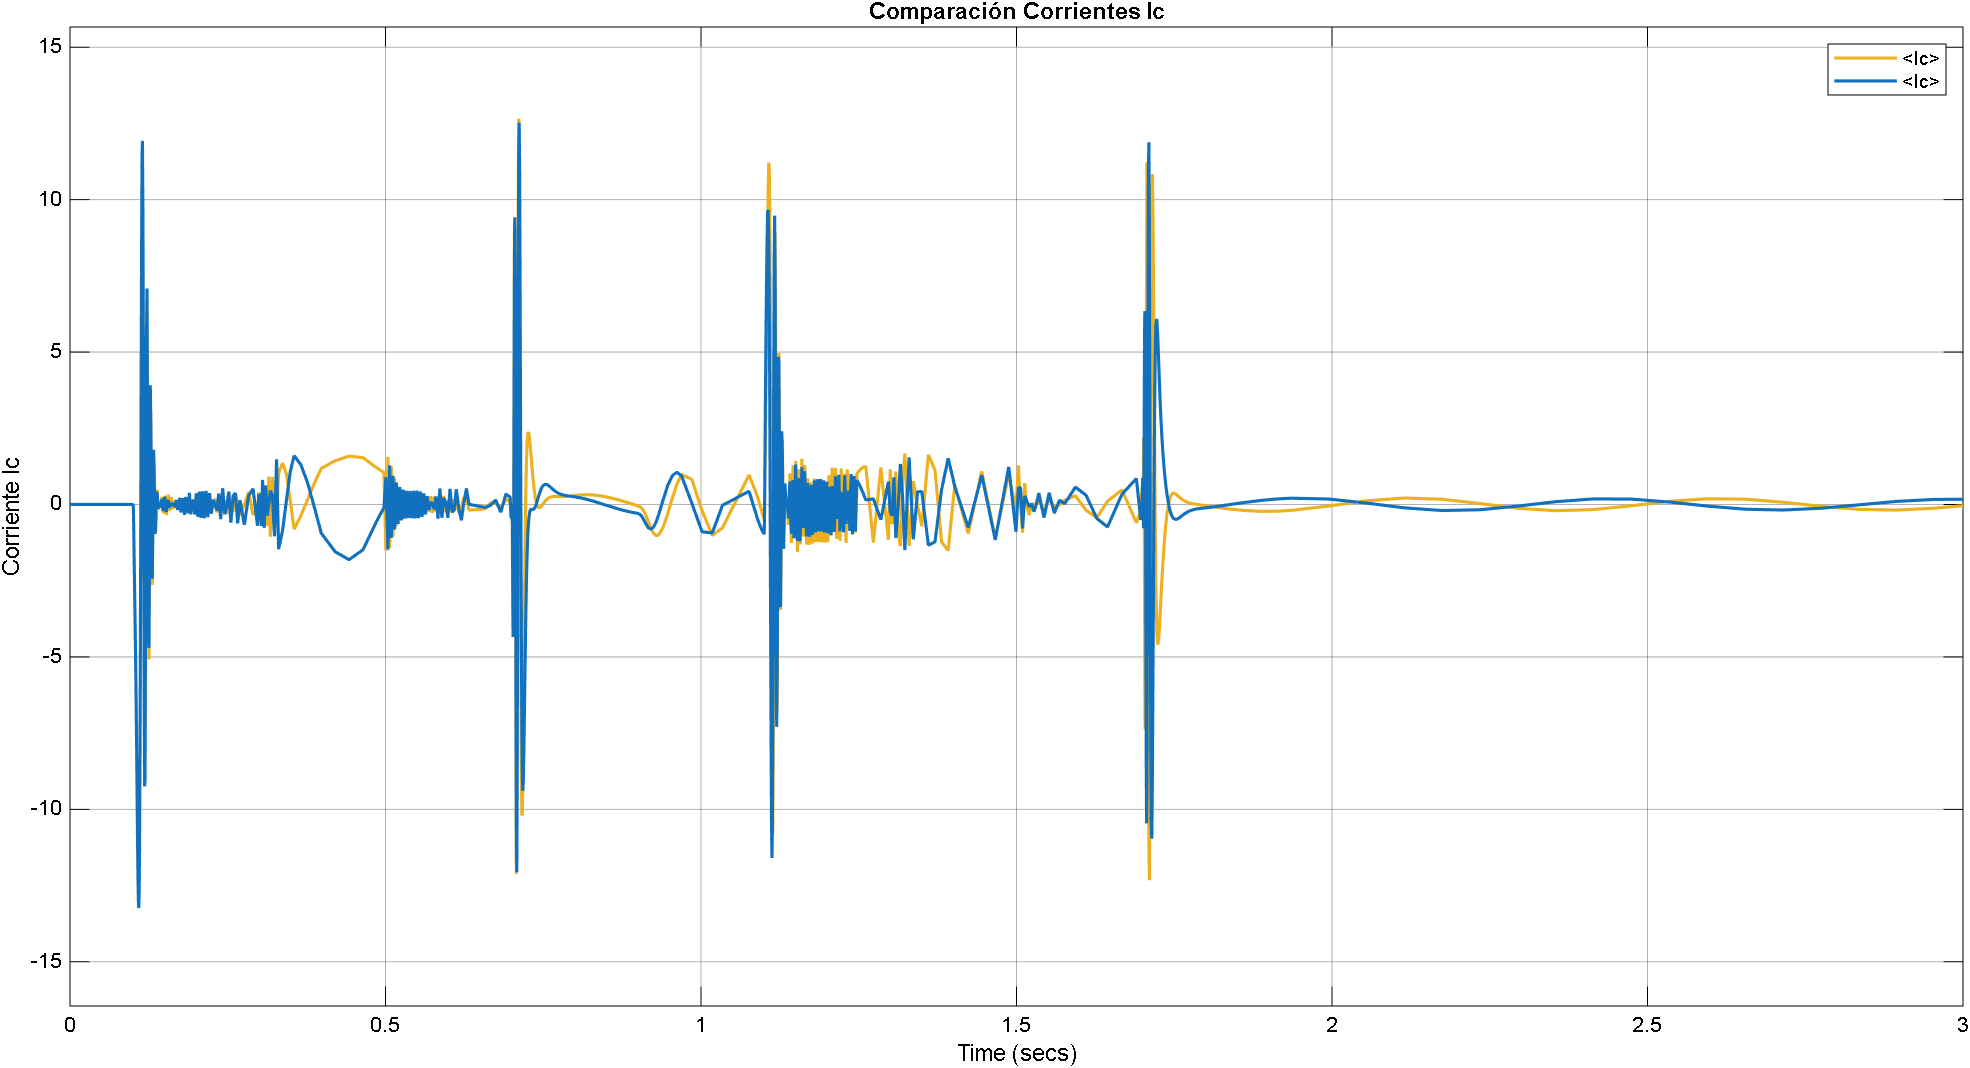
\includegraphics[width=0.86\linewidth,height=0.40\textheight,keepaspectratio]{attachments/Compa_NL_LTI_Ic.png}
    \caption{Evolución temporal de la corriente de fase $i_{cs}(t)$. Se comparan el modelo LTI equivalente aumentado (trazo amarillo) y el modelo no lineal desacoplado mediante realimentación (trazo azul).}
    \label{fig:comparacion-corriente-c}
\end{figure}

\begin{figure}[!htbp]
    \centering
    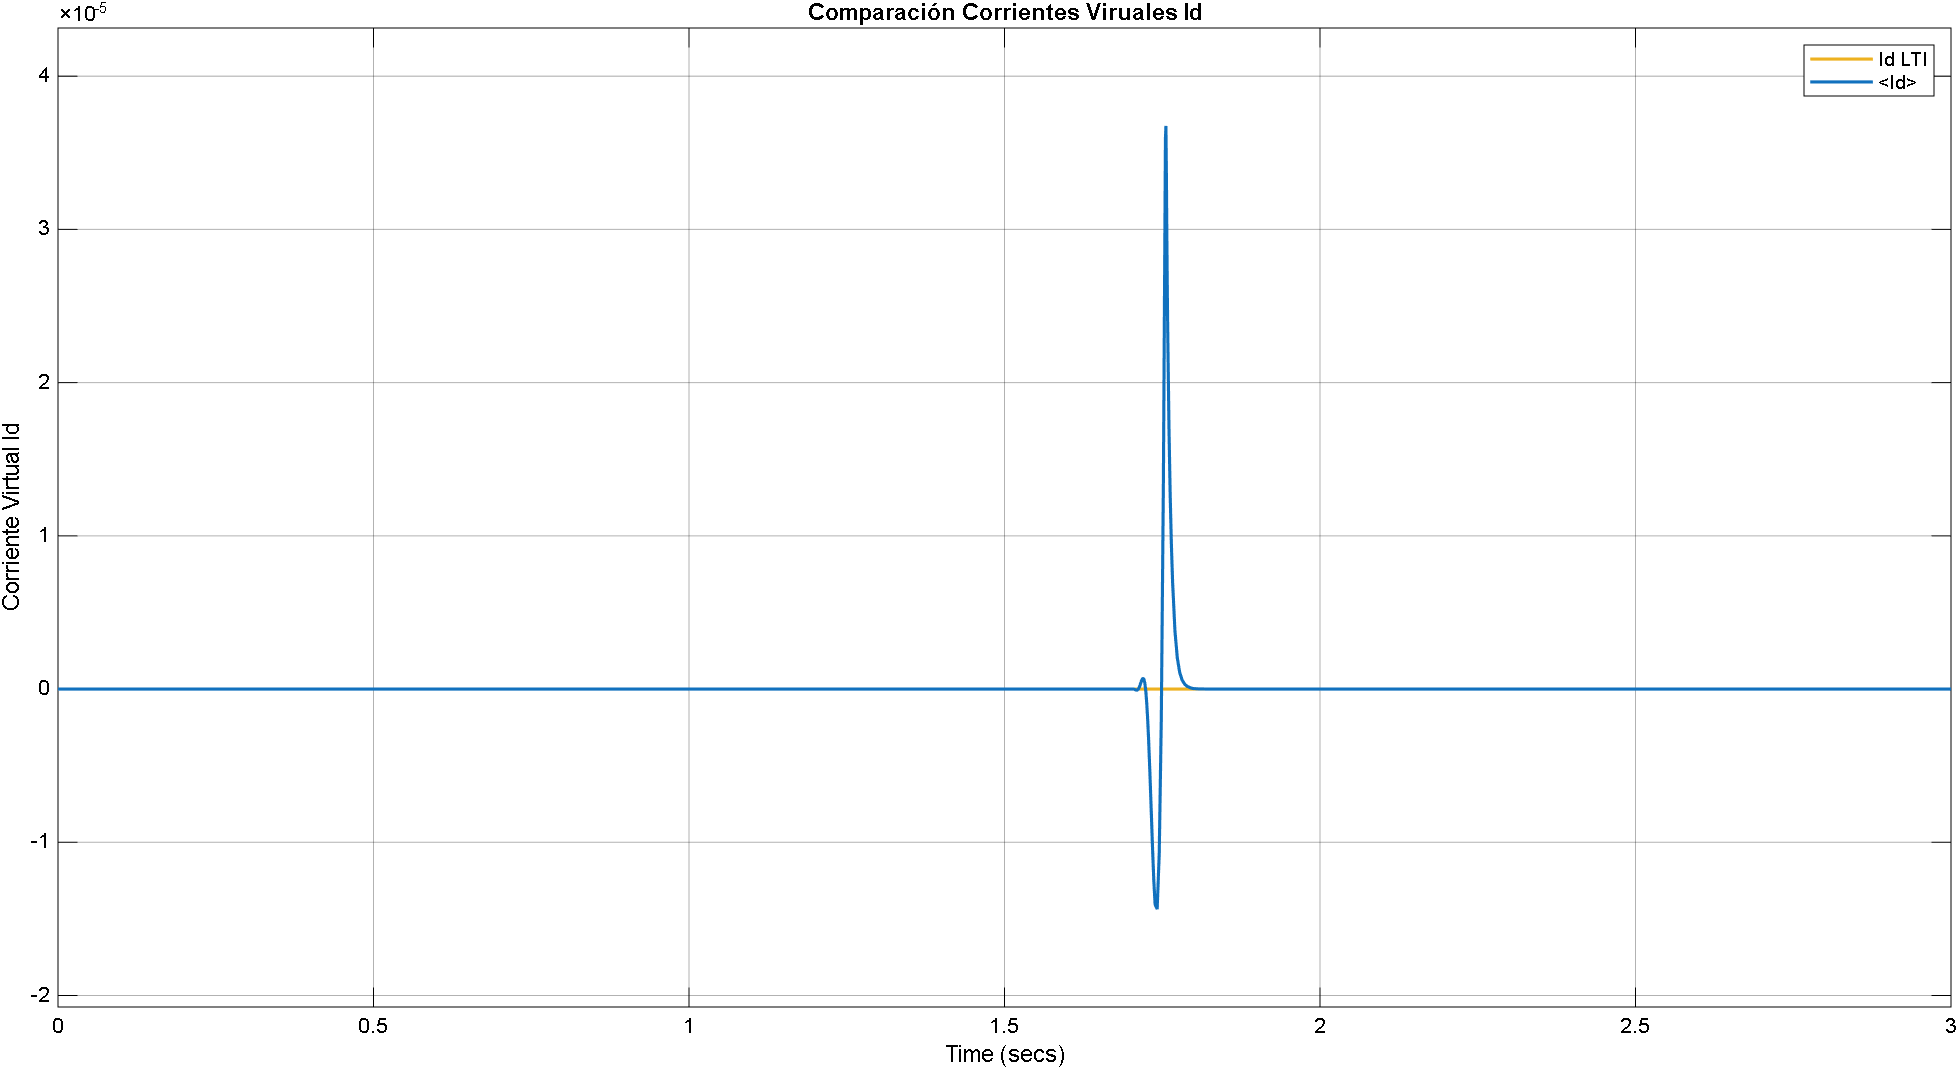
\includegraphics[width=0.86\linewidth,height=0.40\textheight,keepaspectratio]{attachments/Compa_NL_LTI_Id.png}
    \caption{Evolución temporal de la corriente virtual del eje directo $i_{ds}^{r}(t)$: comparación entre el modelo no lineal desacoplado mediante realimentación y el modelo LTI equivalente aumentado.}
    \label{fig:comparacion-corriente-d}
\end{figure}

\begin{figure}[!htbp]
    \centering
    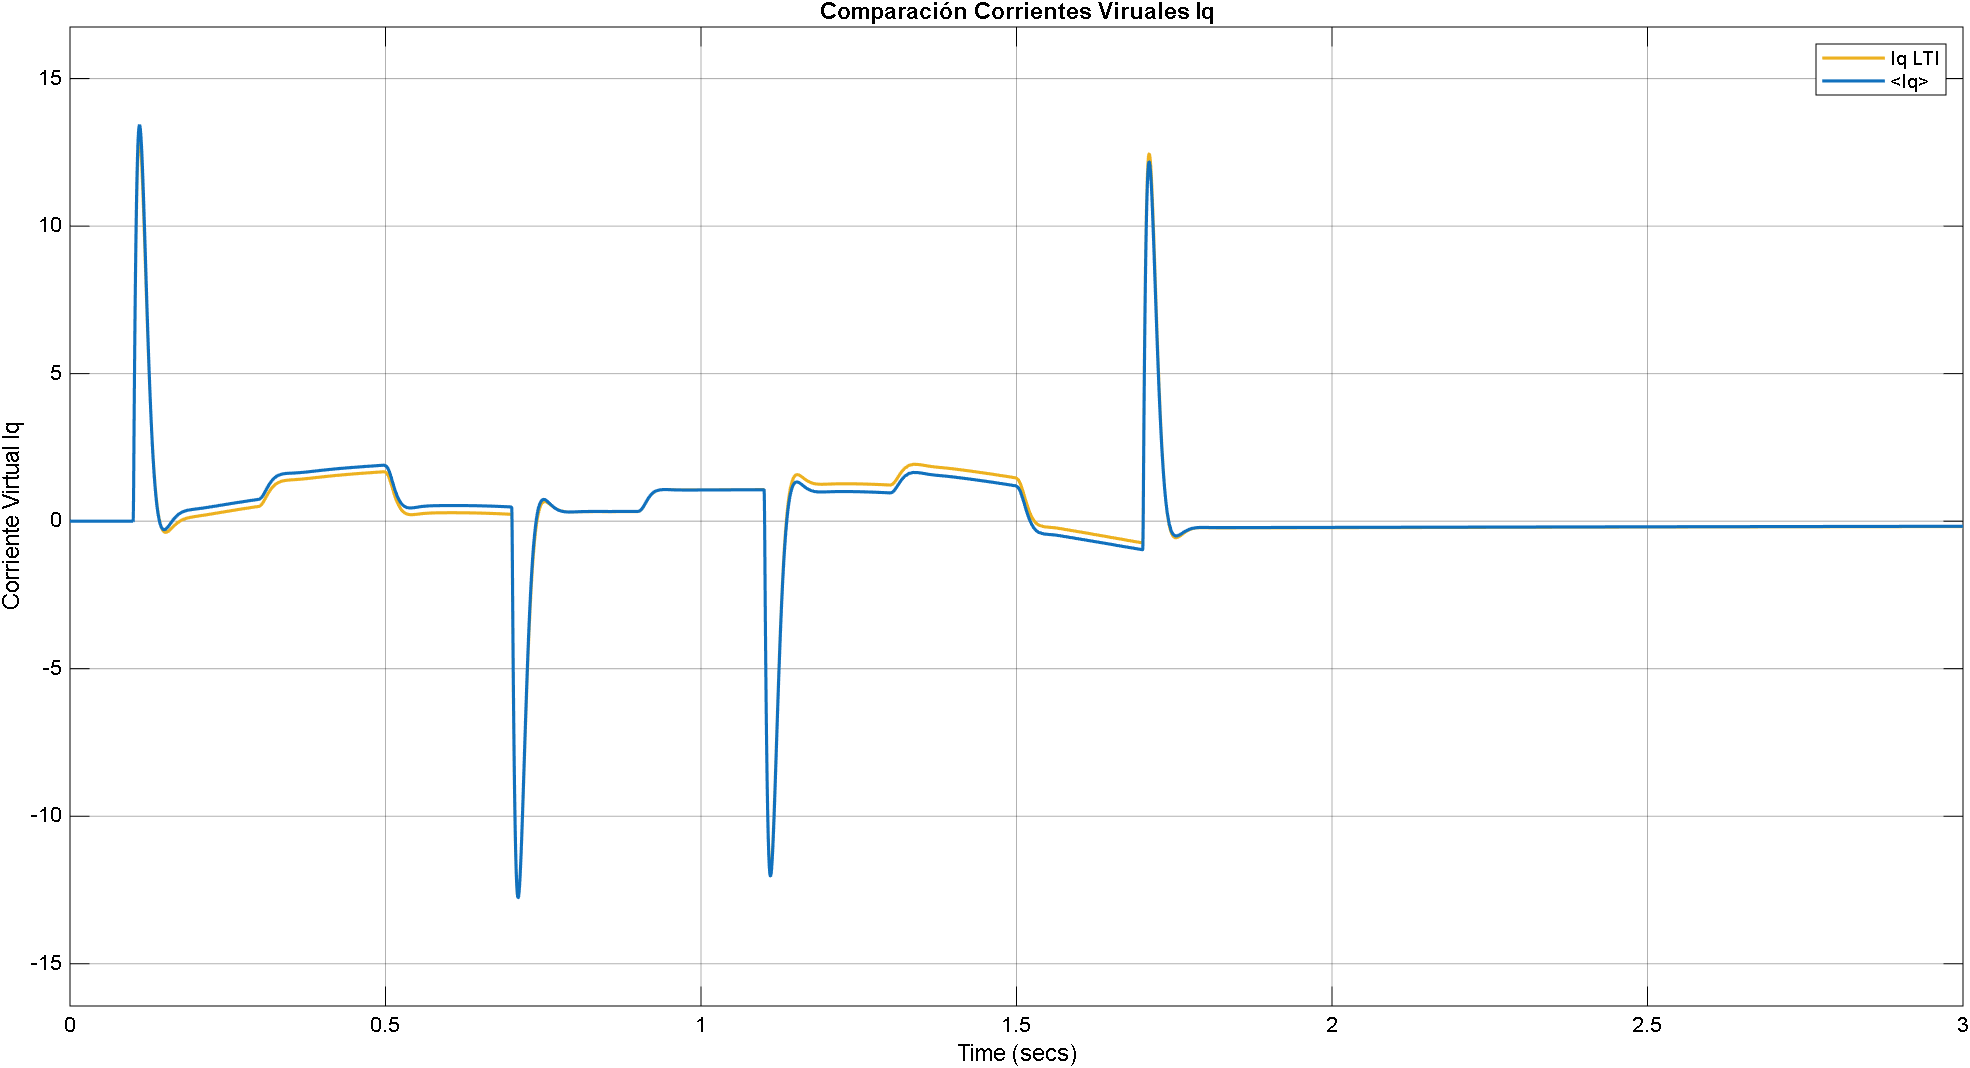
\includegraphics[width=0.86\linewidth,height=0.40\textheight,keepaspectratio]{attachments/Compa_NL_LTI_Iq.png}
    \caption{Evolución temporal de la corriente virtual del eje en cuadratura $i_{qs}^{r}(t)$: comparación entre el modelo no lineal desacoplado mediante realimentación y el modelo LTI equivalente aumentado.}
    \label{fig:comparacion-corriente-q}
\end{figure}



Las corrientes $i^r_{dq0}$ y $i_{abc}$ presentan picos transitorios durante las conmutaciones y cambios de
carga, convergiendo luego a valores cuasi estacionarios acordes al régimen de operación.

\begin{figure}[!htbp]
    \centering
    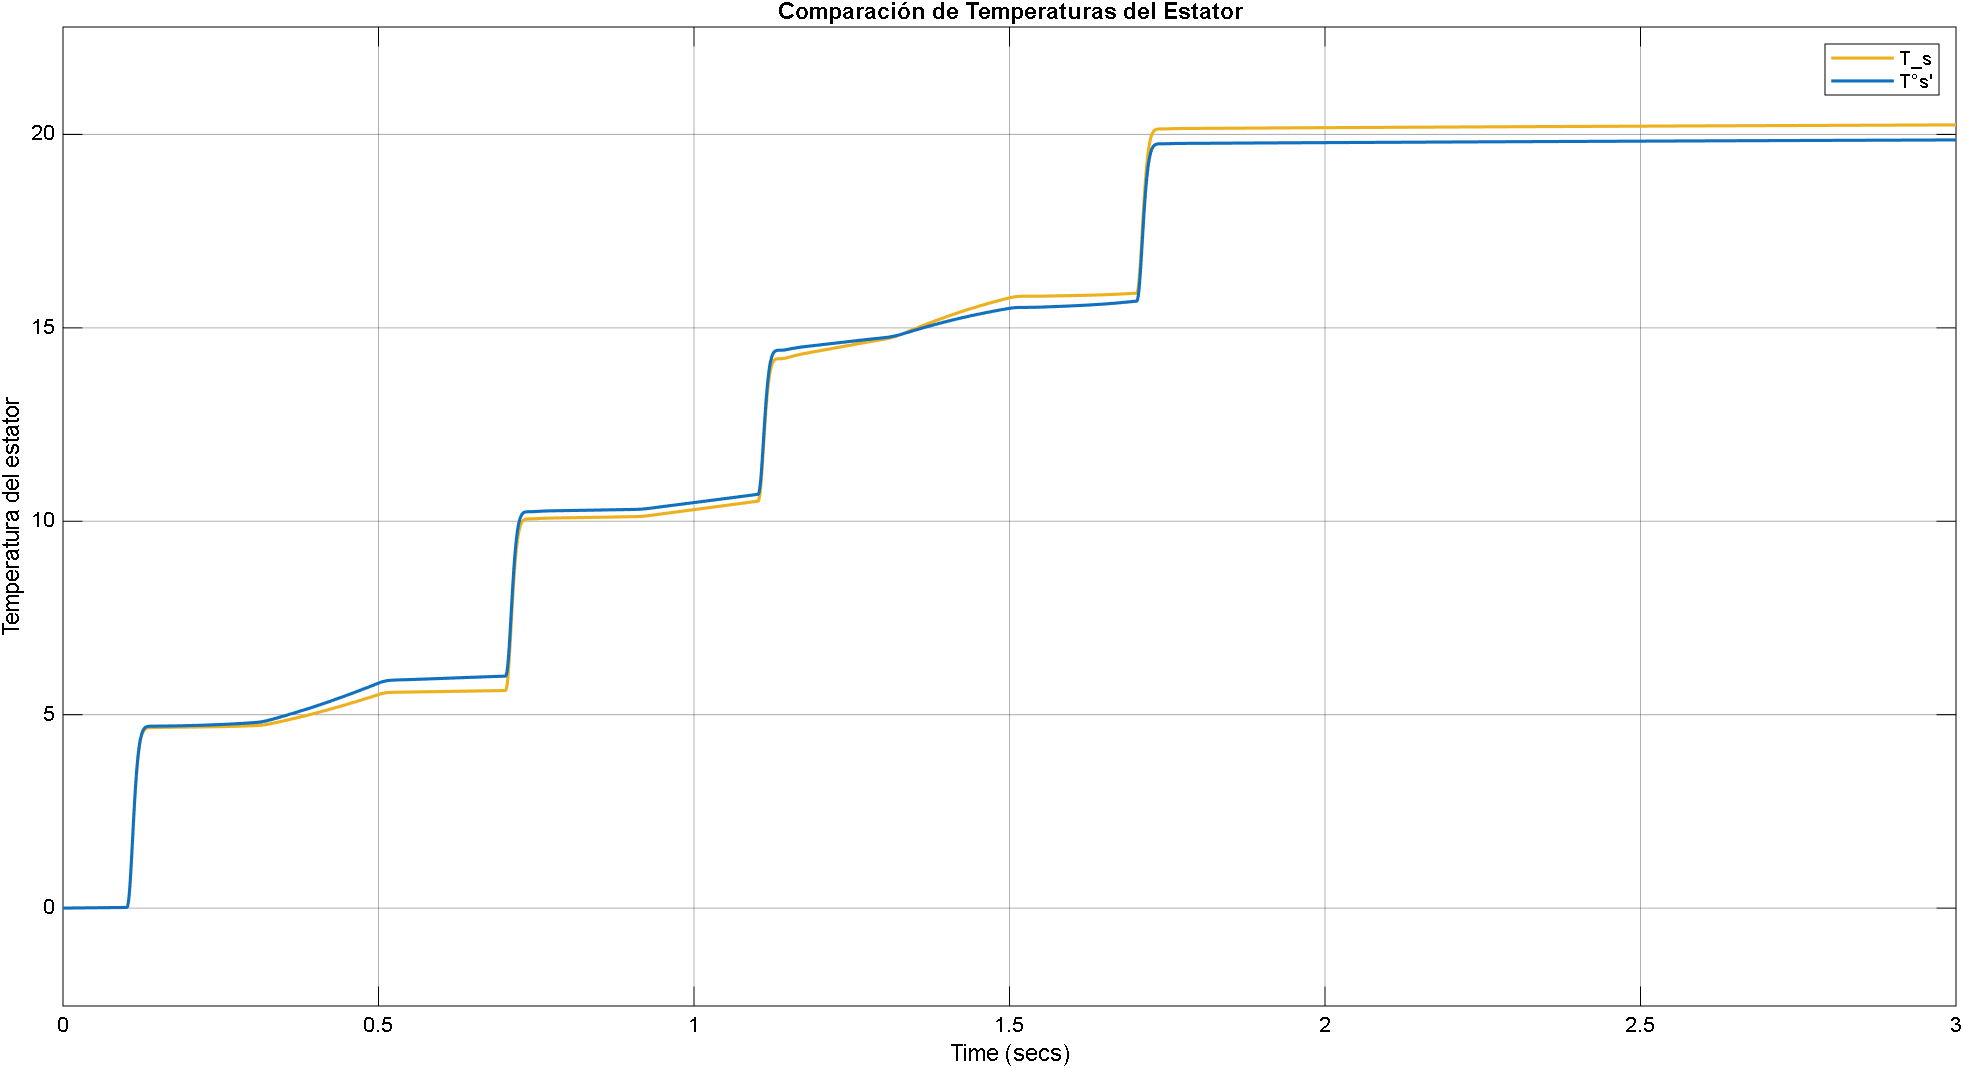
\includegraphics[width=0.86\linewidth,height=0.40\textheight,keepaspectratio]{attachments/Compa_NL_LTI_Temp_estator.png}
    \caption{Evolución temporal de la temperatura del bobinado del estator $T_s^{\circ}(t)$: comparación entre el modelo no lineal desacoplado mediante realimentación y el modelo LTI equivalente aumentado.}
    \label{fig:comparacion-temperatura}
\end{figure}
La temperatura del estator $T_s$ evoluciona de manera mucho más lenta que las variables
eléctricas y mecánicas, aumentando progresivamente debido a las pérdidas resistivas en los bobinados.

Al evaluar los comportamientos de los sistemas muestran que las respuestas dinámicas del modelo no lineal desacoplado mediante realimentación y del modelo LTI equivalente aumentado se encuentran prácticamente superpuestos en $\theta_m$, $\omega_m$ y $T_s$. Esto significa que la linealización realizada alrededor del punto de operación es adecuada y que el modelo LTI captura con alta fidelidad la dinámica dominante del sistema.  

En general las mínimas diferencias se deben a que en el modelo LTI se supuesto la ($R_s$) Resistencia del estator constante pese a que ésta varía con la temperatura del estator que varía con las solicitaciones que se da al motor, como la variación de la Resistencia del estator respecto a la Temperatura es poco significativa. En consecuencia en la situación planteada la aproximación resulta válida pero si se planteara una situación con más exigencias o si las exigencias durarán más tiempo, situaciones en las que se presenta mayor variación de la Temperatura, si tendriamos diferencias más significativa entre ambos modelos.

\paragraph{Curva paramétrica de torque vs velocidad}\mbox{}\\
\begin{figure}[!htbp]
    \centering
    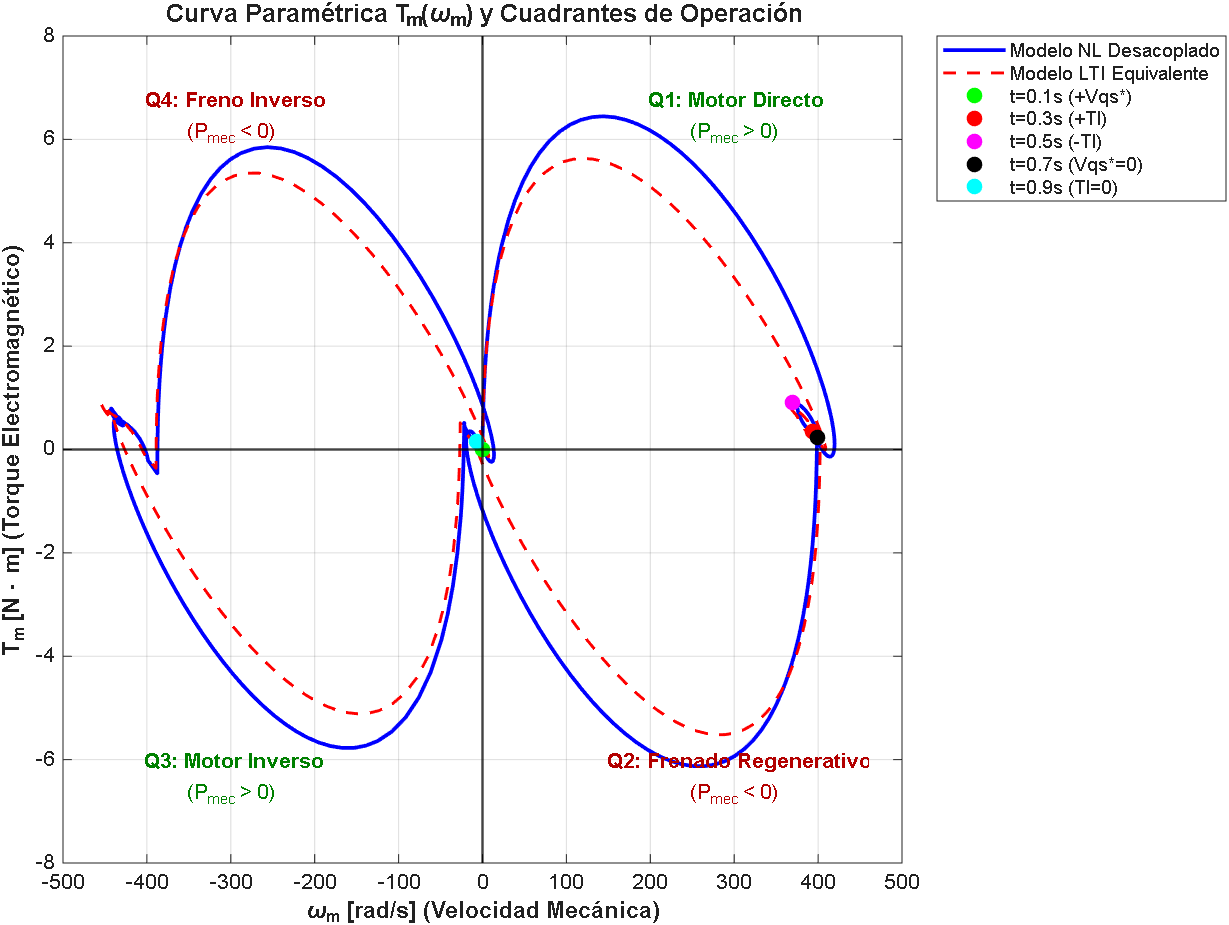
\includegraphics[width=0.75\linewidth]{attachments/Cuadrantes de Operación.png}
    \caption{Trayectoria del torque electromagnético $T_m$ en función de la velocidad angular $\omega_m$ durante el ensayo dinámico, con identificación de los cuatro cuadrantes de operación. Se comparan el modelo no lineal desacoplado (línea azul continua) y el modelo LTI equivalente (línea roja discontinua).}
    \label{fig:cuadrantes-operacion}
\end{figure}


\FloatBarrier
Se procede a analizar la curva $T_m$ vs. $\omega_m$ y se confirma la capacidad del sistema para operar la máquina en los cuatro cuadrantes de manera estable o sea puede funcionar como motor y como freno en ambos sentidos de giro. 
\begin{itemize}
  \item Cuadrante I (Motor Directo, $T_m>0,\; \omega_m>0)$:

  Luego de aplicado el escalón postivo de tensión  en $t=0,1s$ (punto verde), la máquina acelera desde el reposo entregando potencia mecánica positiva hasata estabilizarse cerca de $w_m\sim400\;\frac{rad}{s}$.Durante los escalones de carga en $t=0,3\;s$ (punto rojo) y $t=0,5\;s$ (punto rosa), el sistema permanece en el $1^{er}$cuadrante.  
  \item Cuadrante II (Frenado regenerativo, $T_m<0,\; \omega_m>0)$:

  \nopagebreak[4]
  Cuando se anula la consigna de tensión en $t=0,7\;s$(punto negro) mientras persiste el torque de carga negativo, la máquina reduce su velocidad desarrollando un torque motor negativo que frena el eje y devuelve hacia la fuente.
  \item Cuadrantes III y IV (Motor Inverso y Freno Inverso, ($\omega_m<0$): 

  Al invertir el sentido de giro ($\omega_m<0$), el sistema transita por el $3^{er}$ cuadrante ($T_m<0, \; \omega_m<0, \;$ impulsando en sentido inverso) y por el $4^{to}$cuadrante ($T_m>0, \; \omega_m<0, \;$ frenando el giro inverso) hasta retornar finalmente al origen ($\omega=0,\; T_m=0$) luego de retirar el torque de carga en $t=0,9\;s$ (punto celeste).  
\end{itemize}

\FloatBarrier
\paragraph{Valores de establecimiento}\mbox{}\\
% Código LaTeX para: Resultados dinámicos de la velocidad $\omega_m$ (Modelo NL Desacoplado)
\begin{figure}[!htbp]
    \centering
    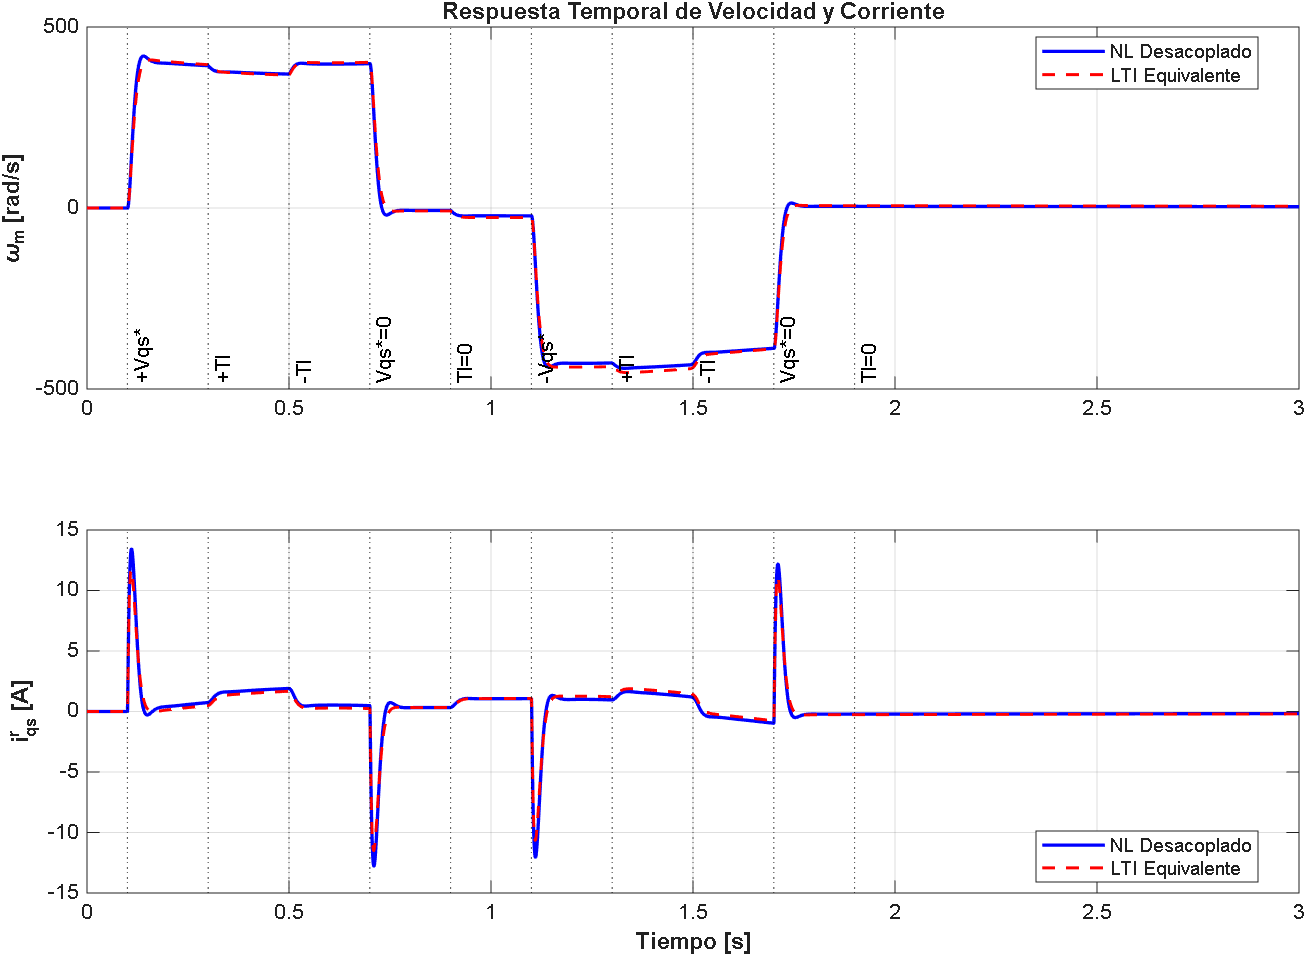
\includegraphics[width=0.75\linewidth]{attachments/NL Desacoplado vs LTI Aumentado transitorio.png}
    \caption{Inicio y fin de crecimiento en $\omega_m$ y $i^r_{qs}$}
    \label{fig:transitorios marcar inicio y fin}
\end{figure}

% Código LaTeX para: Resultados dinámicos de la velocidad $\omega_m$ (Modelo NL Desacoplado)
\begin{table}[htbp]
    \centering
\caption{Resultados dinámicos de la velocidad $\omega_m$ (Modelo NL Desacoplado)}
\begin{tabular}{|c|c|c|c|c|c|c|}
\hline
$t_{event}$ (s) & $y_0$ (\text{rad/s}) & $y_f$ (\text{rad/s}) & $y_{pico}$ (\text{rad/s}) & $\text{RiseTime}_{10-90}$ (s) & $\text{SettlingTime}_{\pm 1\%}$ (s) & $\text{Overshoot}$ (\%) \\
\hline
0.1 & 0.000 & 393.087 & 419.645 & 0.0180 & 0.1389 & 6.76 \\
\hline
0.3 & 391.612 & 369.971 & 369.971 & 0.1280 & 0.1913 & 0.00 \\
\hline
0.5 & 372.255 & 398.721 & 399.847 & 0.0144 & 0.1873 & 4.25 \\
\hline
0.7 & 398.718 & -6.725 & -19.473 & 0.0196 & 0.0580 & 3.14 \\
\hline
0.9 & -7.031 & -21.801 & -22.195 & 0.0175 & 0.1003 & 2.67 \\
\hline
1.1 & -21.802 & -428.069 & -439.555 & 0.0200 & 0.0594 & 2.83 \\
\hline
1.3 & -429.935 & -433.098 & -442.927 & 0.0028 & 0.1947 & 310.70 \\
\hline
1.5 & -430.145 & -387.553 & -387.553 & 0.1412 & 0.1943 & 0.00 \\
\hline
1.7 & -387.548 & 4.561 & 13.695 & 0.0204 & 0.0581 & 2.33 \\
\hline
1.9 & 4.529 & 3.681 & 3.681 & 0.8433 & 1.0772 & 0.00 \\
\hline
\end{tabular}
\end{table}

% Código LaTeX para: Resultados dinámicos de la velocidad $\omega_m$ (Modelo LTI Aumentado)
\begin{table}[htbp]
    \centering
\caption{Resultados dinámicos de la velocidad $\omega_m$ (Modelo LTI Aumentado)}
\begin{tabular}{|c|c|c|c|c|c|c|}
\hline
$t_{event}$ (s) & $y_0$ (\text{rad/s}) & $y_f$ (\text{rad/s}) & $y_{pico}$ (\text{rad/s}) & $\text{RiseTime}_{10-90}$ (s) & $\text{SettlingTime}_{\pm 1\%}$ (s) & $\text{Overshoot}$ (\%) \\
\hline
0.1 & 0.000 & 395.938 & 409.060 & 0.0229 & 0.1508 & 3.31 \\
\hline
0.3 & 394.427 & 367.078 & 367.078 & 0.1265 & 0.1912 & 0.00 \\
\hline
0.5 & 369.352 & 402.475 & 402.475 & 0.0218 & 0.1864 & 0.00 \\
\hline
0.7 & 402.472 & -8.130 & -8.820 & 0.0251 & 0.0450 & 0.17 \\
\hline
0.9 & -8.437 & -26.532 & -26.532 & 0.0250 & 0.1127 & 0.00 \\
\hline
1.1 & -26.533 & -438.171 & -439.672 & 0.0251 & 0.0445 & 0.36 \\
\hline
1.3 & -440.028 & -443.741 & -454.703 & 0.0032 & 0.1947 & 295.19 \\
\hline
1.5 & -440.682 & -389.078 & -389.078 & 0.1398 & 0.1943 & 0.00 \\
\hline
1.7 & -389.069 & 6.439 & 7.346 & 0.0251 & 0.0449 & 0.23 \\
\hline
1.9 & 6.386 & 5.011 & 5.011 & 0.8430 & 1.0770 & 0.00 \\
\hline
\end{tabular}
\end{table}

% Código LaTeX para: Resultados dinámicos de la corriente $i_{qs}^r$ (Modelo NL Desacoplado)
\begin{table}[htbp]
    \centering
\caption{Resultados dinámicos de la corriente $i_{qs}^r$ (Modelo NL Desacoplado)}
\begin{tabular}{|c|c|c|c|c|c|c|}
\hline
$t_{event}$ (s) & $y_0$ (\text{A}) & $y_f$ (\text{A}) & $y_{pico}$ (\text{A}) & $\text{RiseTime}_{10-90}$ (s) & $\text{SettlingTime}_{\pm 1\%}$ (s) & $\text{Overshoot}$ (\%) \\
\hline
0.1 & 0.000 & 0.740 & 13.430 & 0.0004 & 0.1968 & 1715.51 \\
\hline
0.3 & 0.757 & 1.899 & 1.899 & 0.1222 & 0.1910 & 0.00 \\
\hline
0.5 & 1.885 & 0.481 & 0.448 & 0.0195 & 0.1852 & 2.34 \\
\hline
0.7 & 0.433 & 0.329 & -12.764 & 0.0001 & 0.1286 & 12503.72 \\
\hline
0.9 & 0.331 & 1.064 & 1.077 & 0.0228 & 0.0846 & 1.75 \\
\hline
1.1 & 1.055 & 0.958 & -12.028 & 0.0001 & 0.1984 & 13398.81 \\
\hline
1.3 & 0.977 & 1.210 & 1.651 & 0.0069 & 0.1944 & 189.16 \\
\hline
1.5 & 1.153 & -0.970 & -0.970 & 0.1361 & 0.1941 & 0.00 \\
\hline
1.7 & -0.883 & -0.215 & 12.186 & 0.0004 & 0.0864 & 1856.70 \\
\hline
1.9 & -0.214 & -0.174 & -0.174 & 0.8432 & 1.0772 & 0.00 \\
\hline
\end{tabular}
\end{table}

% Código LaTeX para: Resultados dinámicos de la corriente $i_{qs}^r$ (Modelo LTI Aumentado)
\begin{table}[htbp]
    \centering
\caption{Resultados dinámicos de la corriente $i_{qs}^r$ (Modelo LTI Aumentado)}
\begin{tabular}{|c|c|c|c|c|c|c|}
\hline
$t_{event}$ (s) & $y_0$ (\text{A}) & $y_f$ (\text{A}) & $y_{pico}$ (\text{A}) & $\text{RiseTime}_{10-90}$ (s) & $\text{SettlingTime}_{\pm 1\%}$ (s) & $\text{Overshoot}$ (\%) \\
\hline
0.1 & 0.000 & 0.485 & 11.732 & 0.0003 & 0.1977 & 2318.71 \\
\hline
0.3 & 0.502 & 1.668 & 1.668 & 0.1231 & 0.1912 & 0.00 \\
\hline
0.5 & 1.655 & 0.240 & 0.240 & 0.0253 & 0.1846 & 0.00 \\
\hline
0.7 & 0.193 & 0.331 & -11.498 & 0.0070 & 0.1515 & 0.00 \\
\hline
0.9 & 0.332 & 1.079 & 1.079 & 0.0285 & 0.1091 & 0.00 \\
\hline
1.1 & 1.070 & 1.223 & -10.653 & 0.0059 & 0.1980 & 0.00 \\
\hline
1.3 & 1.240 & 1.461 & 1.886 & 0.0070 & 0.1945 & 191.78 \\
\hline
1.5 & 1.405 & -0.762 & -0.762 & 0.1354 & 0.1941 & 0.00 \\
\hline
1.7 & -0.675 & -0.262 & 11.139 & 0.0003 & 0.1283 & 2760.55 \\
\hline
1.9 & -0.260 & -0.204 & -0.204 & 0.8430 & 1.0770 & 0.00 \\
\hline
\end{tabular}
\end{table}


Observamos que los pulsos de tensión $v^r_{qs}$ tienen mayor influencia en los cambios de $\omega_ m$ y los pulsos de torque de carga $T_{ld}$ implican cambios mayores en $i^r_{ds}$. Es posible identificar que al aplicarse el torque de carga, la corriente sufre un aumento para compensar dicho torque, mientras que la velocidad decae. Analizando vemos que en ambas variables los transitorios que poseen son similares.

\subsubsection{Comparación de comportamiento de $i^r_{ds}$ con distintos valores iniciales}

Al imponer una condición inicial no nula en el eje directo ($i_{ds}^r(0) = \pm 0.5\text{ A}$) manteniendo activa la ley de control de desacoplamiento NL (que fuerza $v_{ds}^{r*} = -L_q \omega_r i_{qs}^r$), se observan los siguientes efectos en ambos modelos:

\begin{figure}[!htbp]
    \centering
    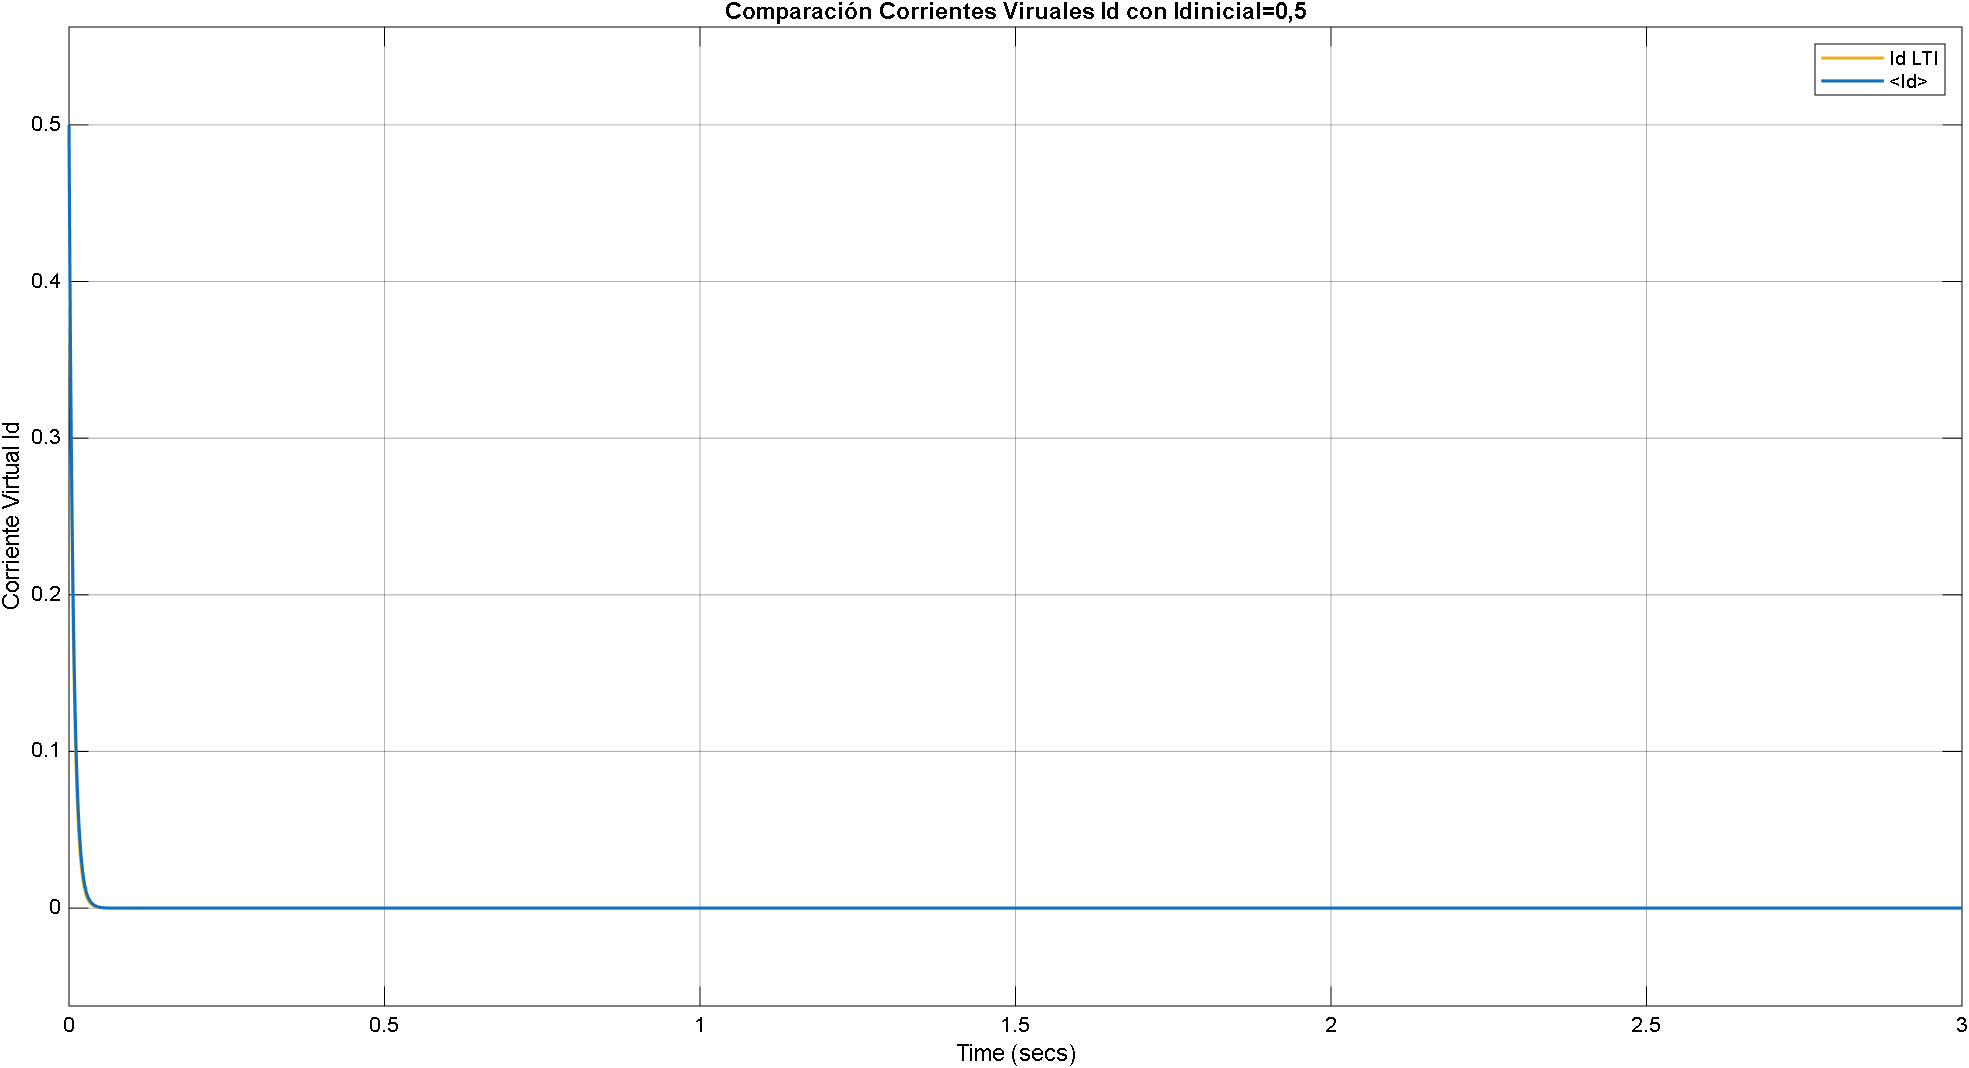
\includegraphics[width=0.86\linewidth,height=0.40\textheight,keepaspectratio]{attachments/Compa_NL_LTI_Id con Id0=05.png}
    \caption{Comportamiento de $i^r_{ds}$ con $i^r_{ds_{inicial}}=0,5\;A$}
    \label{fig:corriente-d-inicial-positiva}
    \par\medskip
    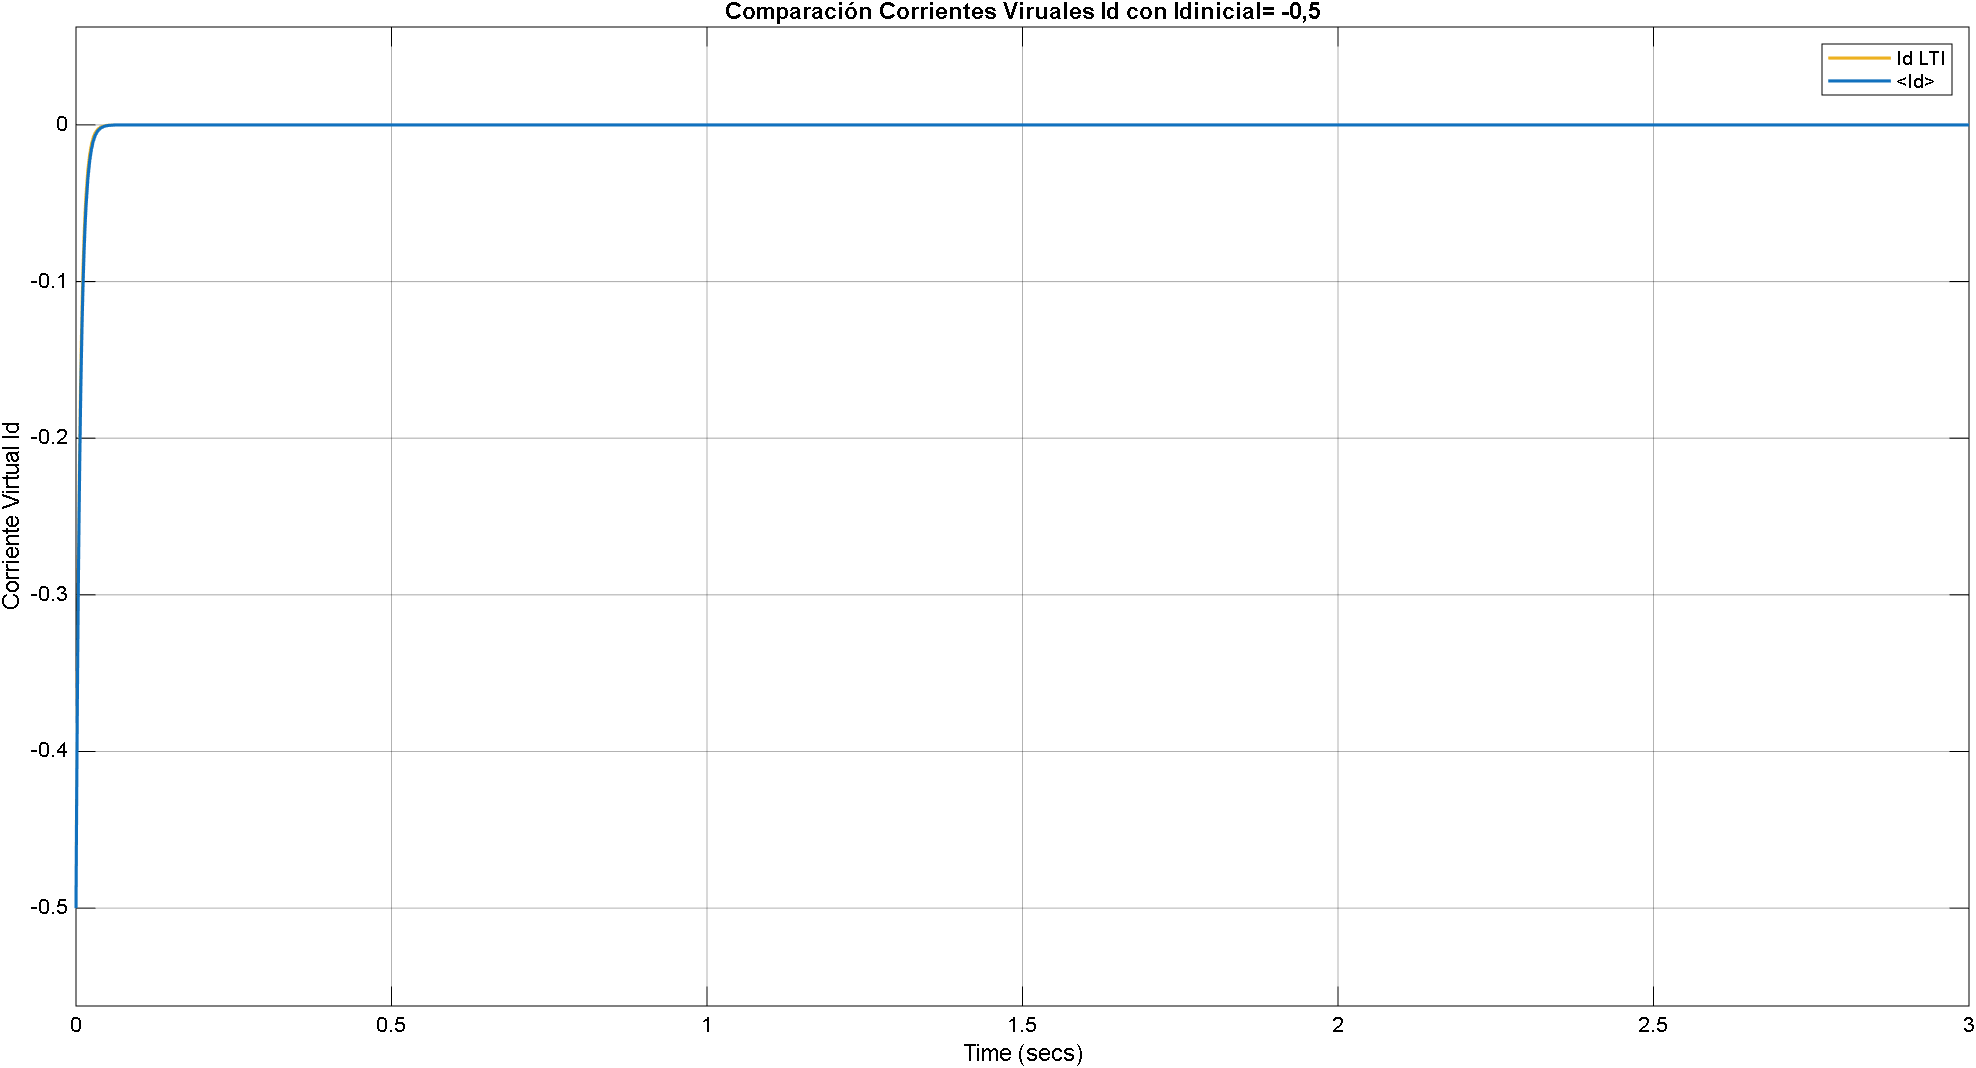
\includegraphics[width=0.86\linewidth,height=0.40\textheight,keepaspectratio]{attachments/Compa_NL_LTI_Id con Id0=-05.png}
    \caption{Comportamiento de $i^r_{ds}$ con $i^r_{ds_{inicial}}=-0,5\;A$}
    \label{fig:corriente-d-inicial-negativa}
\end{figure}

\subsubsection*{Efecto de la condición inicial $i_{ds}^r(0) = \pm 0.5\text{ A}$ frente a $i_{ds}^r(0) = 0\text{ A}$}

Al imponer $i_{ds}^r(0) = \pm 0.5\text{ A}$ con el control de desacoplamiento activo, se concluye que:


    En ambos modelos (NL y LTI), la corriente directa decae a cero con comportamiento de $1^{er}$ orden con constante de tiempo $\tau_d = L_d / R_s \approx 6.5\text{ ms}$. En $\sim 32\text{ ms}$ ($5\tau_d$) ya se extinguió por completo, mucho antes del primer escalón de tensión en $t = 0.1\text{ s}$. La diferencia entre modelos es imperceptible y se debe solo a la leve variación térmica de $R_s(T_s^\circ)$.

     En el modelo LTI el eje $d$ está totalmente desacoplado, por lo que no hay efecto alguno. En el modelo NL, tanto la ley de desacoplamiento completo en eje $q$ como el hecho de que el motor esté detenido ($\omega_r = 0$, $i_{qs}^r = 0$) durante los primeros $0.1\text{ s}$ anulan cualquier torque de reluctancia o tensión cruzada residual.


\subsubsection{Comportamiento de los sistemas con consignas de tensión en el eje $d$}

\paragraph{Modelo LTI equivalente aumentado}
Primeramente se debe recordar que se ha desacoplado al modelo LTI equivalente aumentado del eje $d$ a través de la ley complementaria \eqref{eq:ley-minima}, como ahora queremos darle una consigna por ende quedaría $v^r_{ds}=v^{r*}_{ds}-L_qP_pi^r_{qs}\omega_m$ por consecuencia queda:
\begin{align*}
        \frac{di_{ds}^{r}(t)}{dt} & = \frac{1}{L_{d}} \left[v_{ds}^{r}(t) - R_{s}^{\ell} i_{ds}^{r}(t) + L_{q}P_{p} i_{qs}^{r}(t) \omega_{m}(t) \right]
        \\
        \frac{di_{ds}^{r}(t)}{dt} & = \frac{1}{L_{d}} \Big[\Big(v^{r*}_{ds} -   L_{q}P_{p} i_{qs}^{r}(t) \omega_{m}(t) \Big) - R_{s}^{\ell} i_{ds}^{r}(t) + L_{q}P_{p} i_{qs}^{r}(t) \omega_{m}(t) \Big]
        \\
        \frac{di_{ds}^{r}(t)}{dt} & = \frac{1}{L_{d}} \Big[ v^{r*}_{ds} \cancel{ -  L_{q}P_{p} i_{qs}^{r}(t) \omega_{m}(t)  } - R_{s}^{\ell}{i_{ds}^{r}(t) } + \cancel{ L_{q}P_{p} i_{qs}^{r}(t) \omega_{m}(t)  }\Big] 
    \end{align*}
Ahora se evaluará el comportamiento con las siguientes consignas escalón de $v^{r*}_{ds}$:
\begin{figure}[!htbp]
    \centering
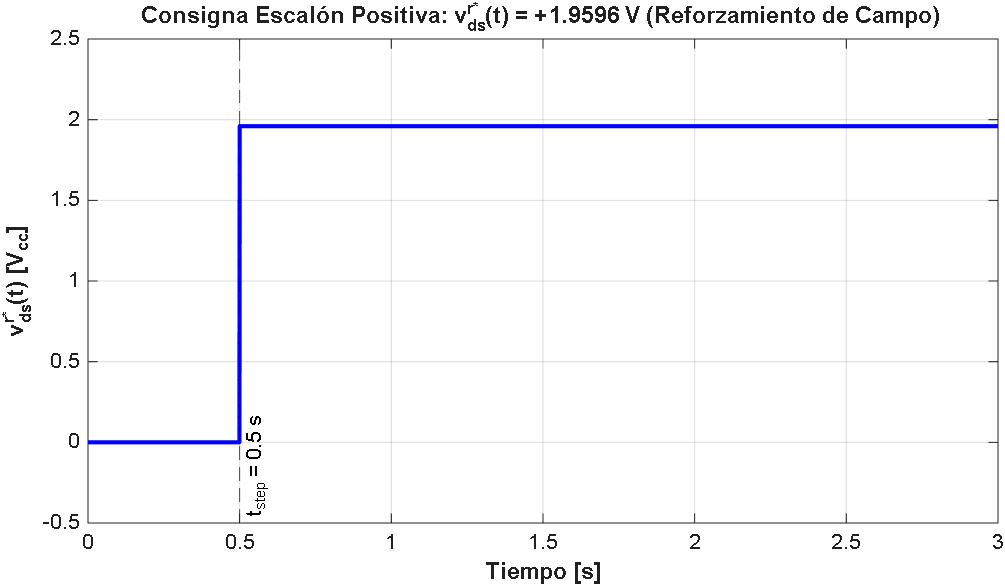
\includegraphics[width=0.5\linewidth]{attachments/Consigna vds Positiva.png}
    \caption{Consigna escalón de $v^{r*}_{ds}$ positiva en $t=0,5\;s$}
    \label{fig:consiga positiva de vds}
    \par\medskip
    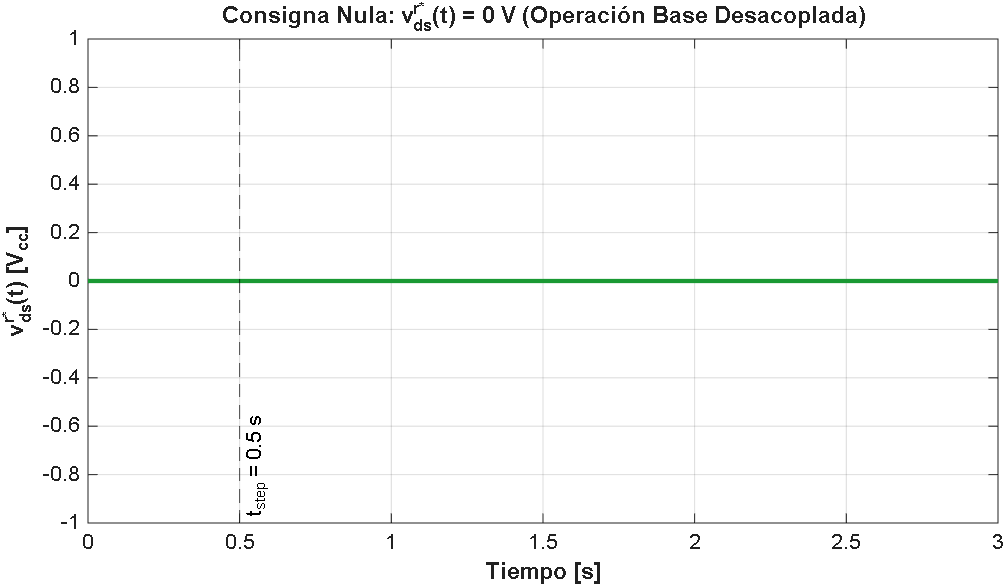
\includegraphics[width=0.5\linewidth]{attachments/Consigna vds Nula.png}
    \caption{Consigna de $v^{r*}_{ds}$ nula}
    \label{fig:consigna nula de vds}
    \par\medskip
    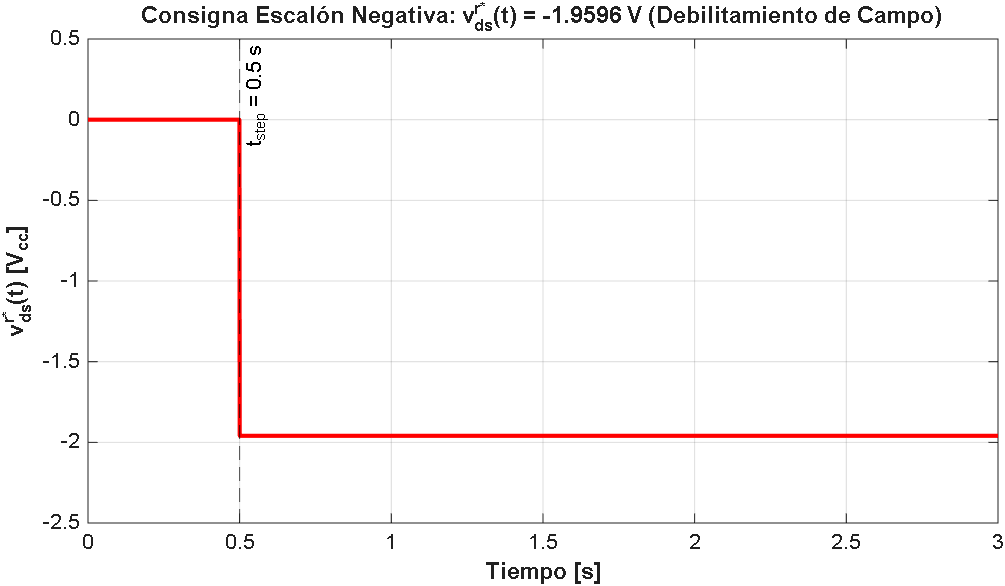
\includegraphics[width=0.5\linewidth]{attachments/Consigna vds Negativa.png}
    \caption{Consigna escalón de $v^{r*}_{ds}$ negativa en $t=0,5\;s$}
    \label{fig:consiga negativa de vds}
\end{figure}
En las siguientes imágenes se verá el comportamiento de distintas variables del Modelo LTI equivalente aumentado con las distintas consignas de $v_{ds}^{r}*$, primero se verá aquellas en las que es indistinta la consigna de $v^{r*}_{ds}$ y luego aquellas en las que el comportamiento varía:
\FloatBarrier
\paragraph{Variables invariantes con la consigna}
Las curvas de posición, velocidad y corriente en cuadratura prácticamente se superponen para las tres consignas de tensión del eje directo.
\begin{figure}[!htbp]
    \centering
    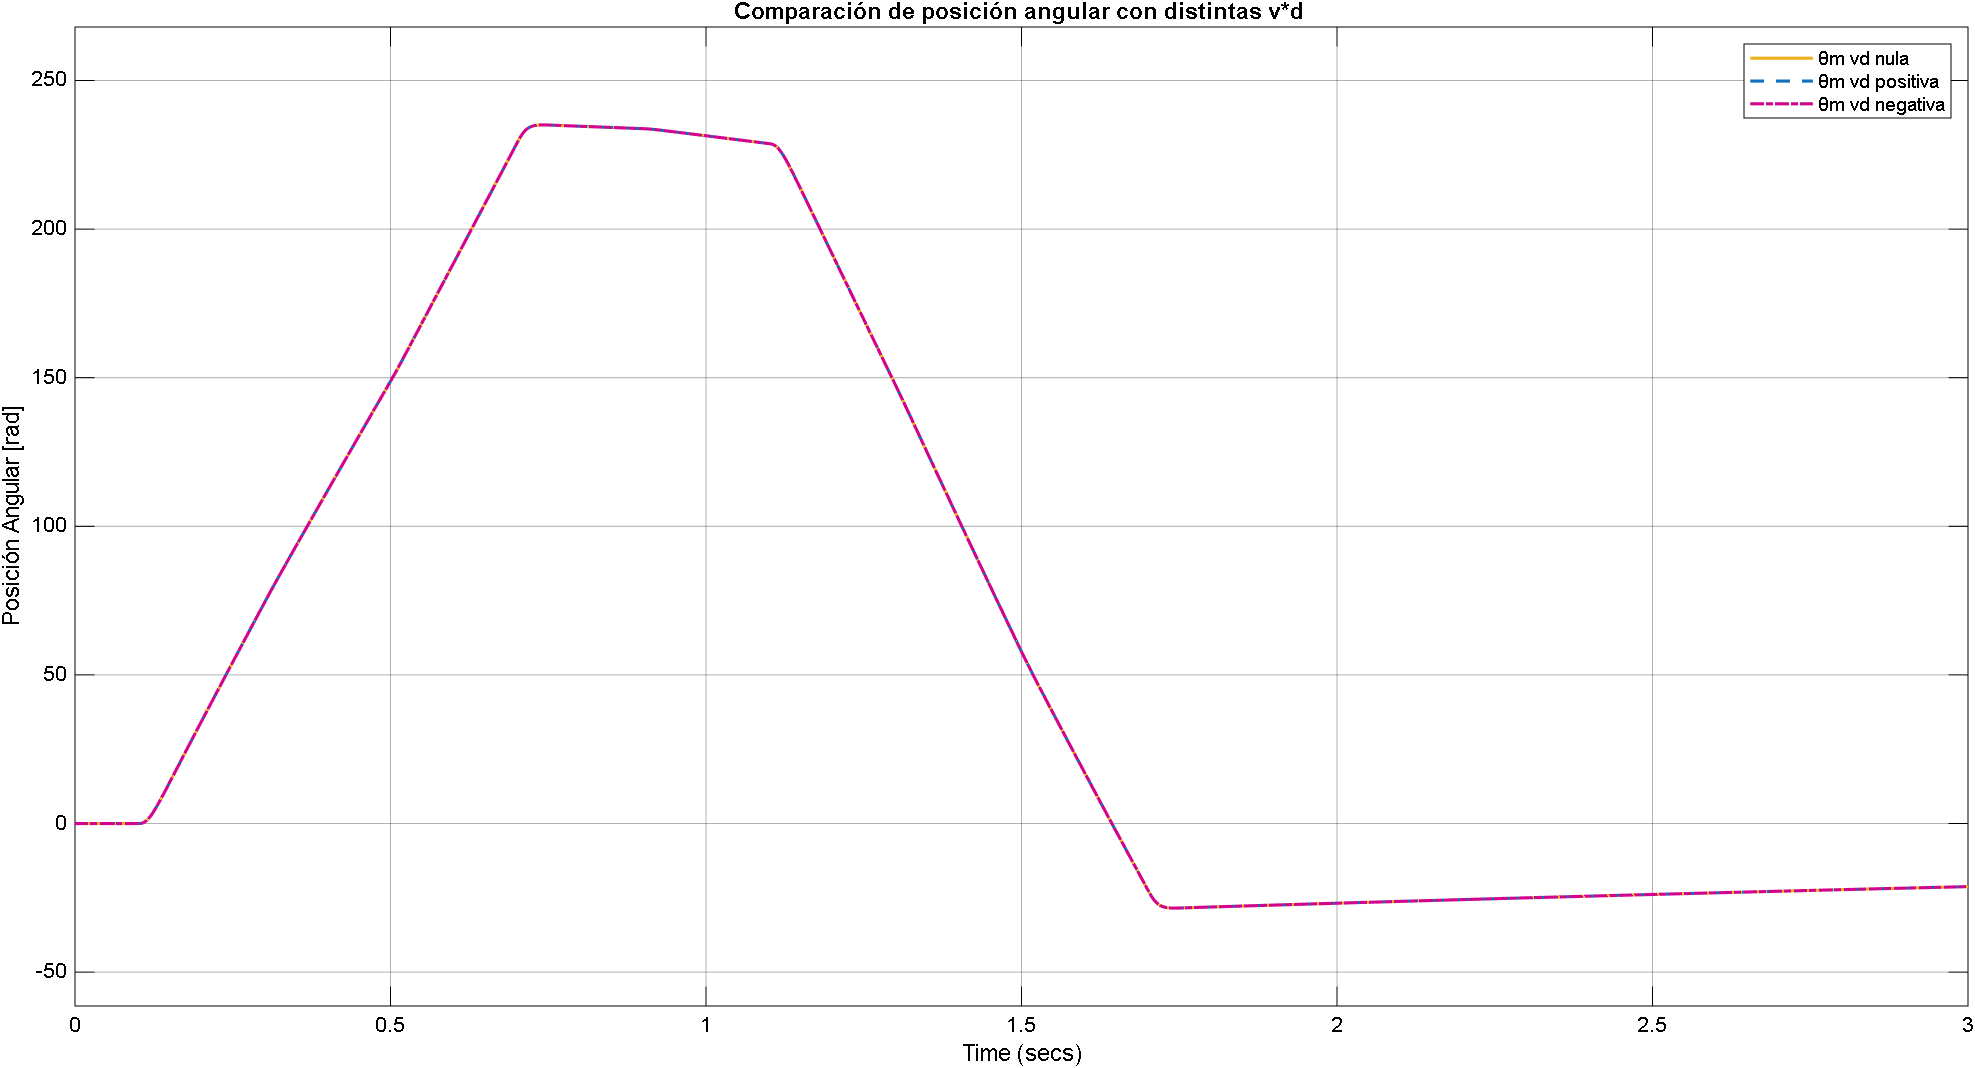
\includegraphics[width=0.86\linewidth,height=0.40\textheight,keepaspectratio]{attachments/Compa_consigna_vd_posici_ang.png}
    \caption{Comparación del comportamiento de la posición angular con las distintas consignas de $v_{ds}^{r*}$ en el modelo LTI equivalente aumentado }
    \label{fig:comparacion posicion ang con consigna vd LTI}
\end{figure}
\begin{figure}[!htbp]
    \centering
    % El título y la unidad originales corresponden a posición; la leyenda identifica las curvas como velocidad.
    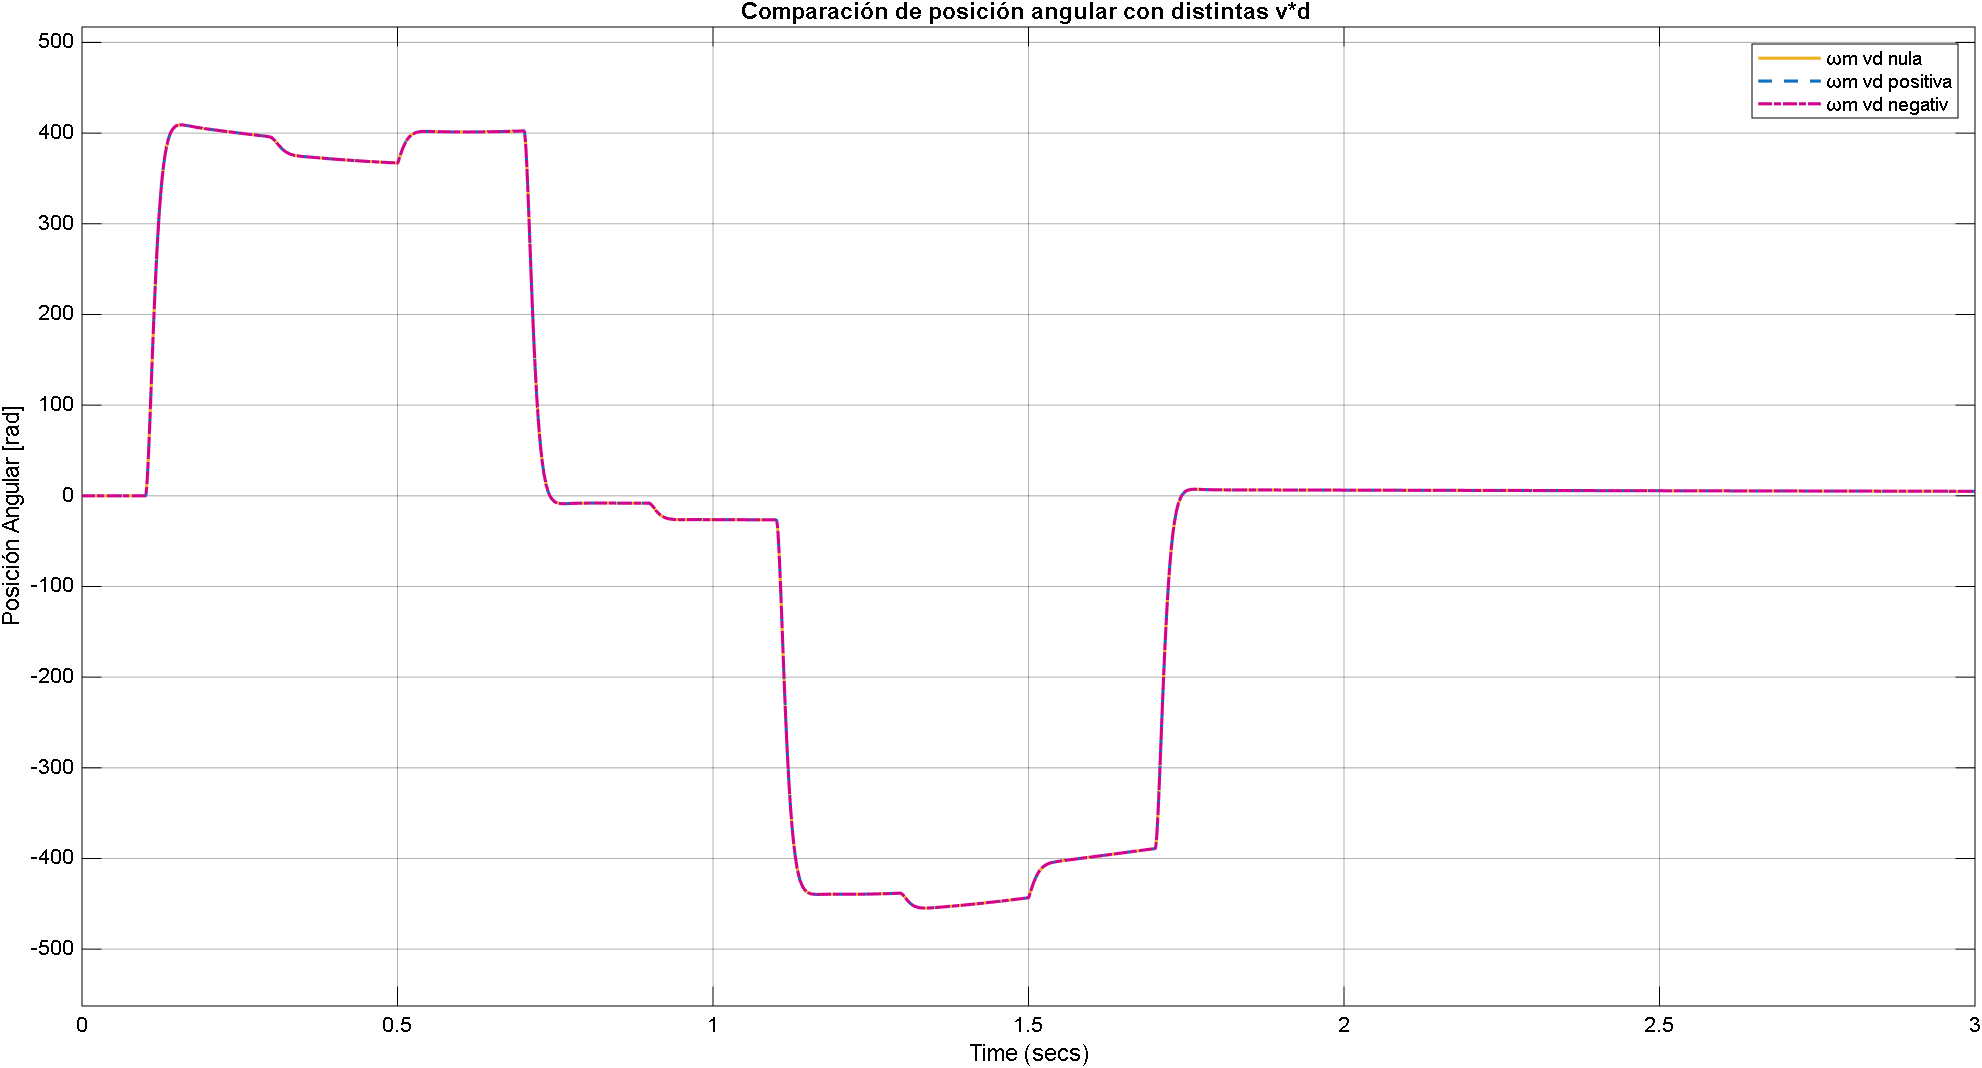
\includegraphics[trim=12bp 0 0 12bp,clip,width=0.86\linewidth,height=0.40\textheight,keepaspectratio]{attachments/Compa_consigna_vd_velocidad_ang.png}
    \caption{Velocidad angular $\omega_m$ (rad/s) del modelo LTI equivalente aumentado para las tres consignas de $v_{ds}^{r*}$.}
    \label{fig:comparacion velocidad ang con consigna vd LTI}
\end{figure}
\begin{figure}[!htbp]
    \centering
    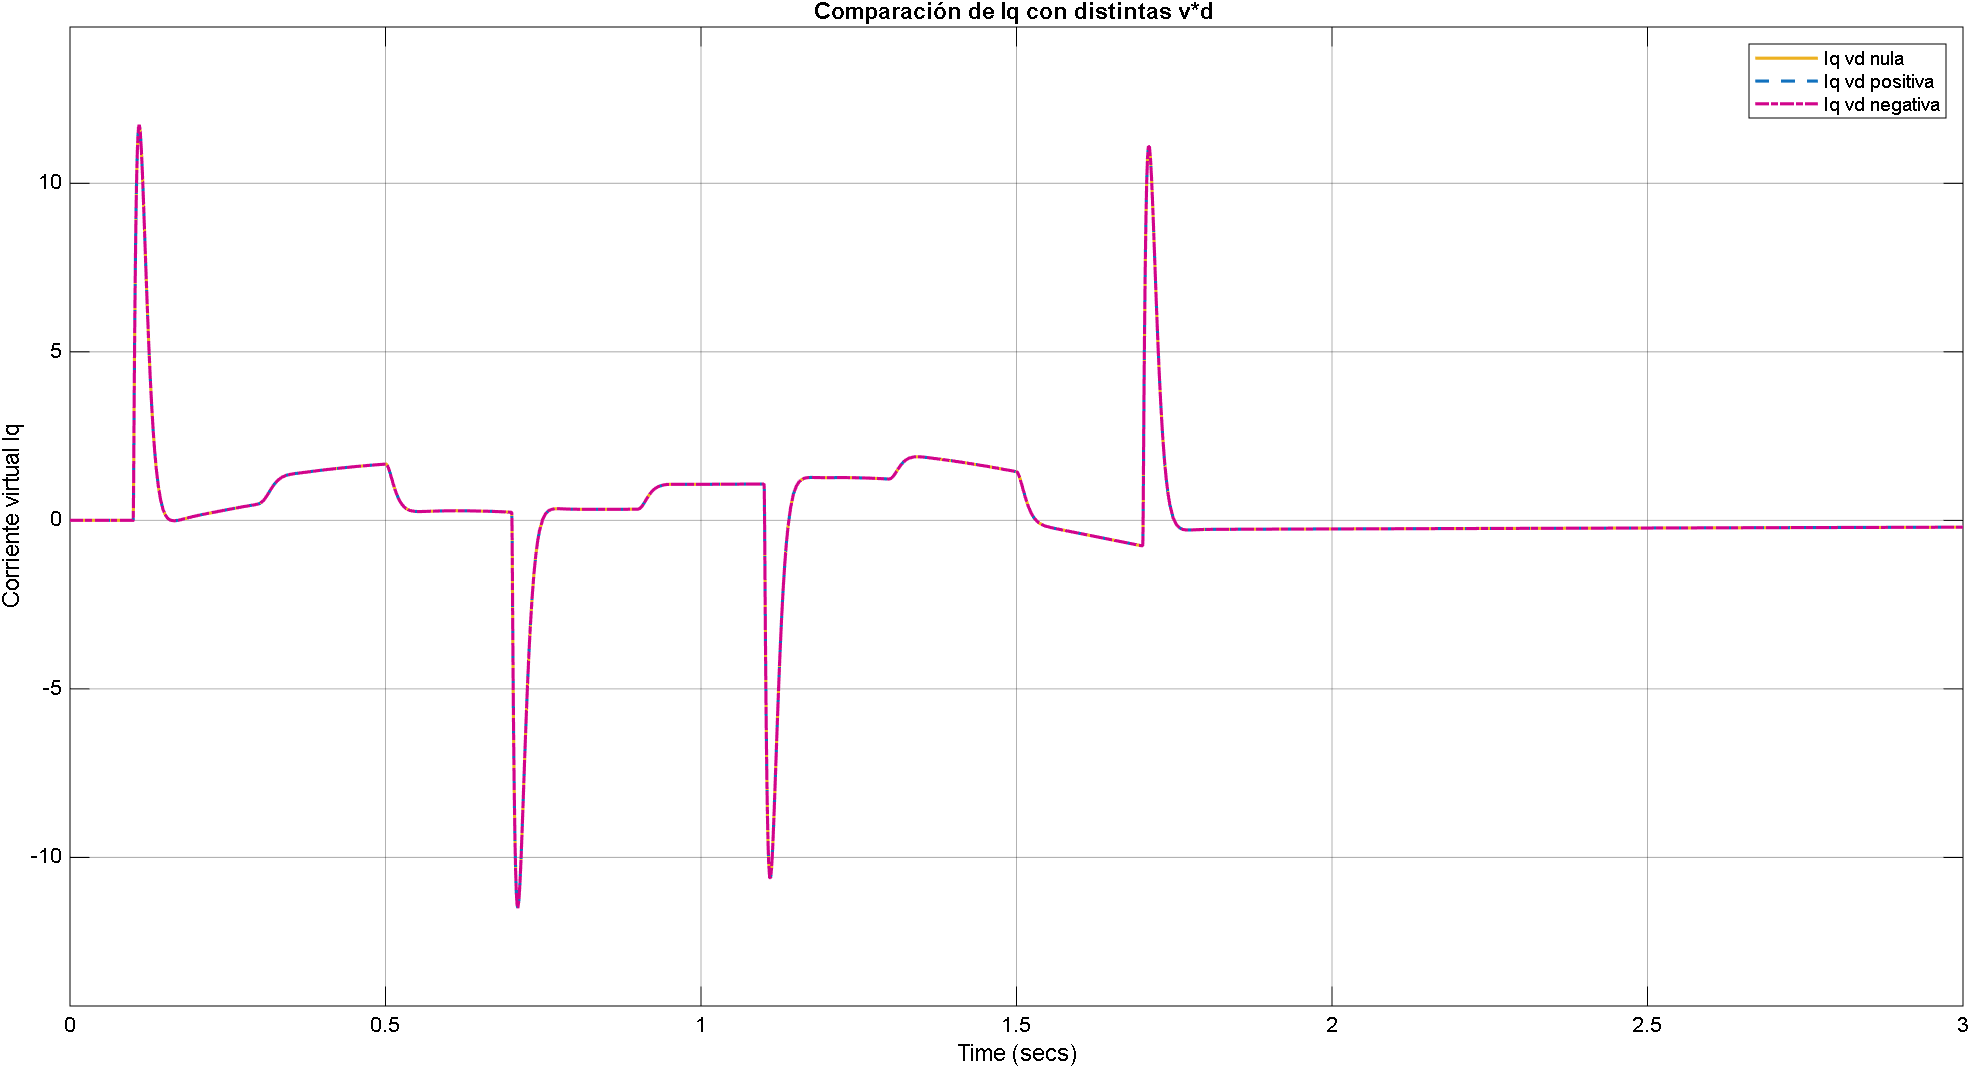
\includegraphics[width=0.86\linewidth,height=0.40\textheight,keepaspectratio]{attachments/Compa_consigna_vd_Iq.png}
    \caption{Comparación del comportamiento de la corriente virtual Iq con las distintas consignas de $v_{ds}^{r*}$}
    \label{fig:comparacion Iq con consigna vd}
\end{figure}
\FloatBarrier
\paragraph{Variables que varían con la consigna}
\begin{figure}[!htbp]
    \centering
    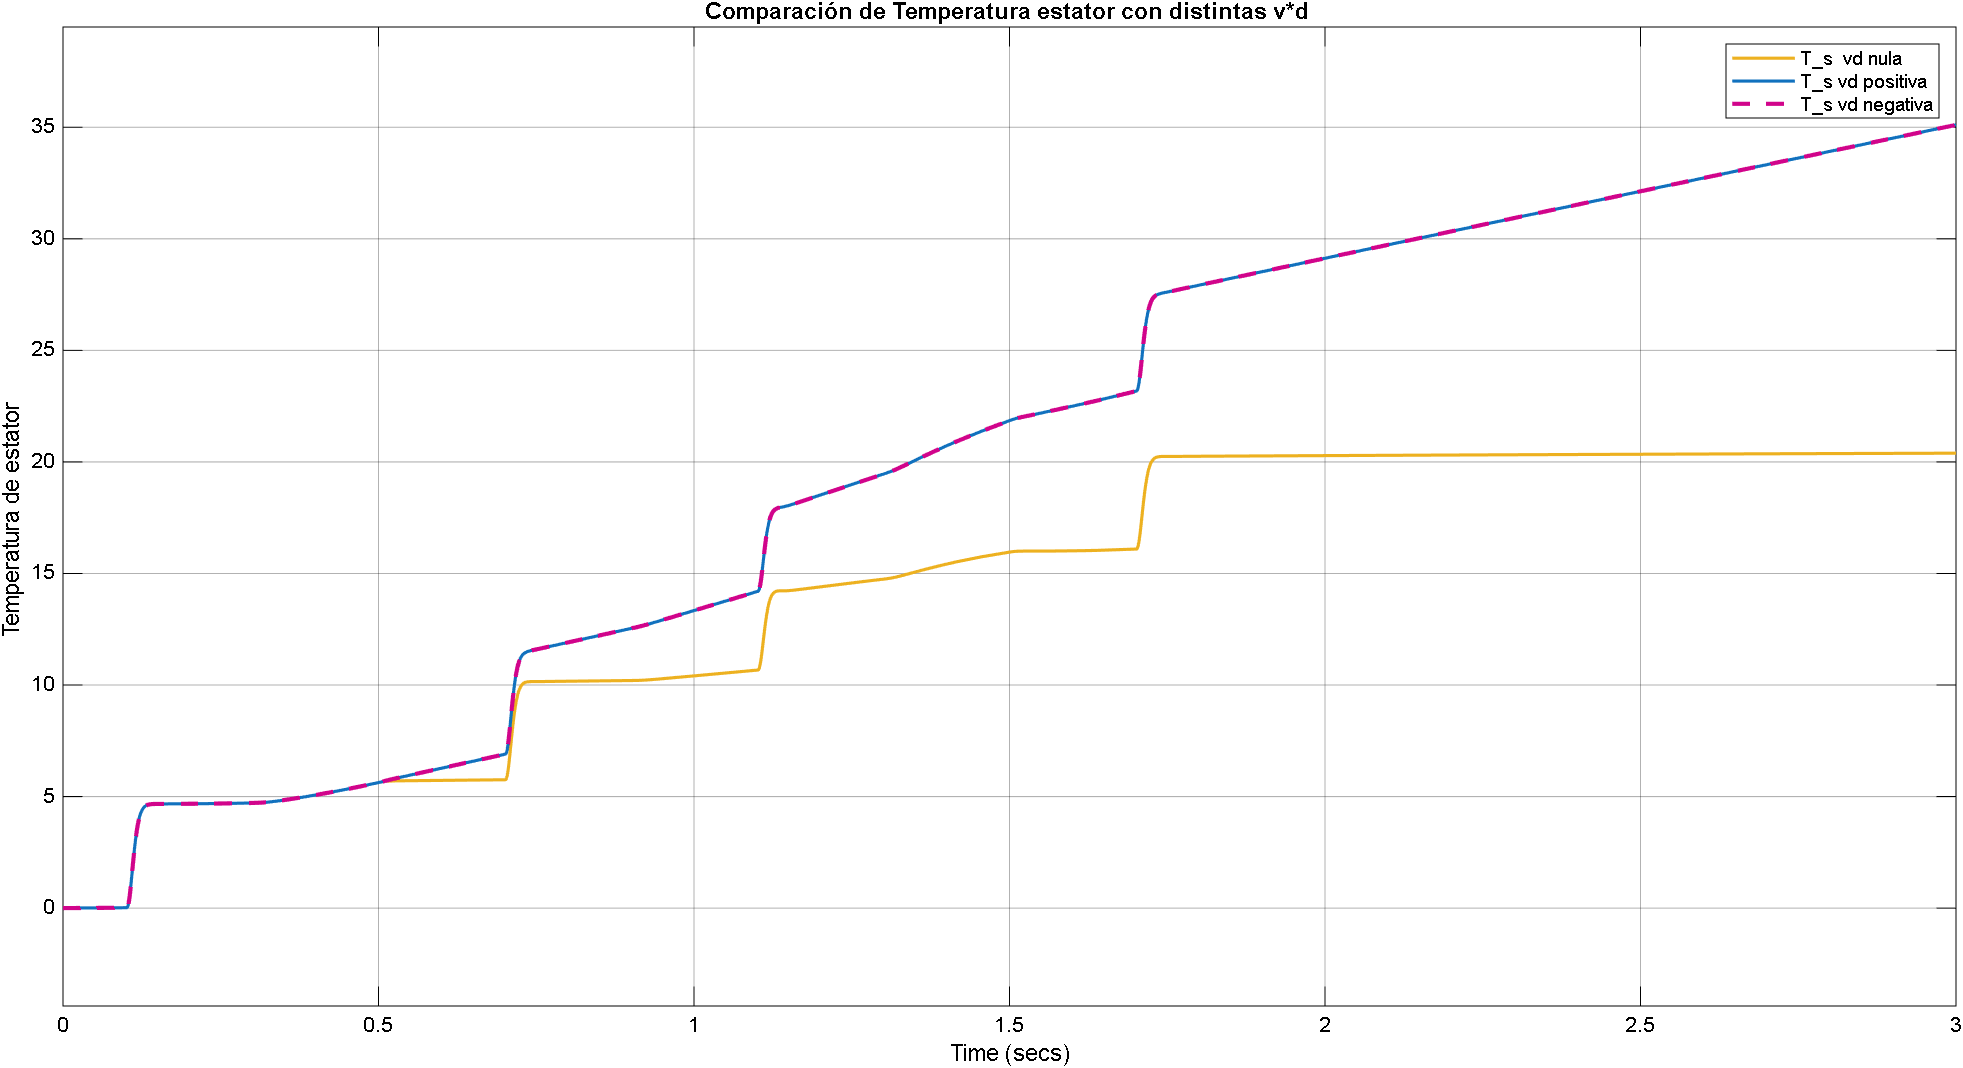
\includegraphics[width=0.86\linewidth,height=0.40\textheight,keepaspectratio]{attachments/Compa_consigna_vd_tempe_estator.png}
    \caption{Comparación del comportamiento de la Temperatura del estator con las distintas consignas de $v_{ds}^{r*}$ en el modelo LTI equivalente aumentada}
    \label{fig:comparacion Temp estator con consigna vd LTI}
\end{figure}
\begin{figure}[!htbp]
    \centering
    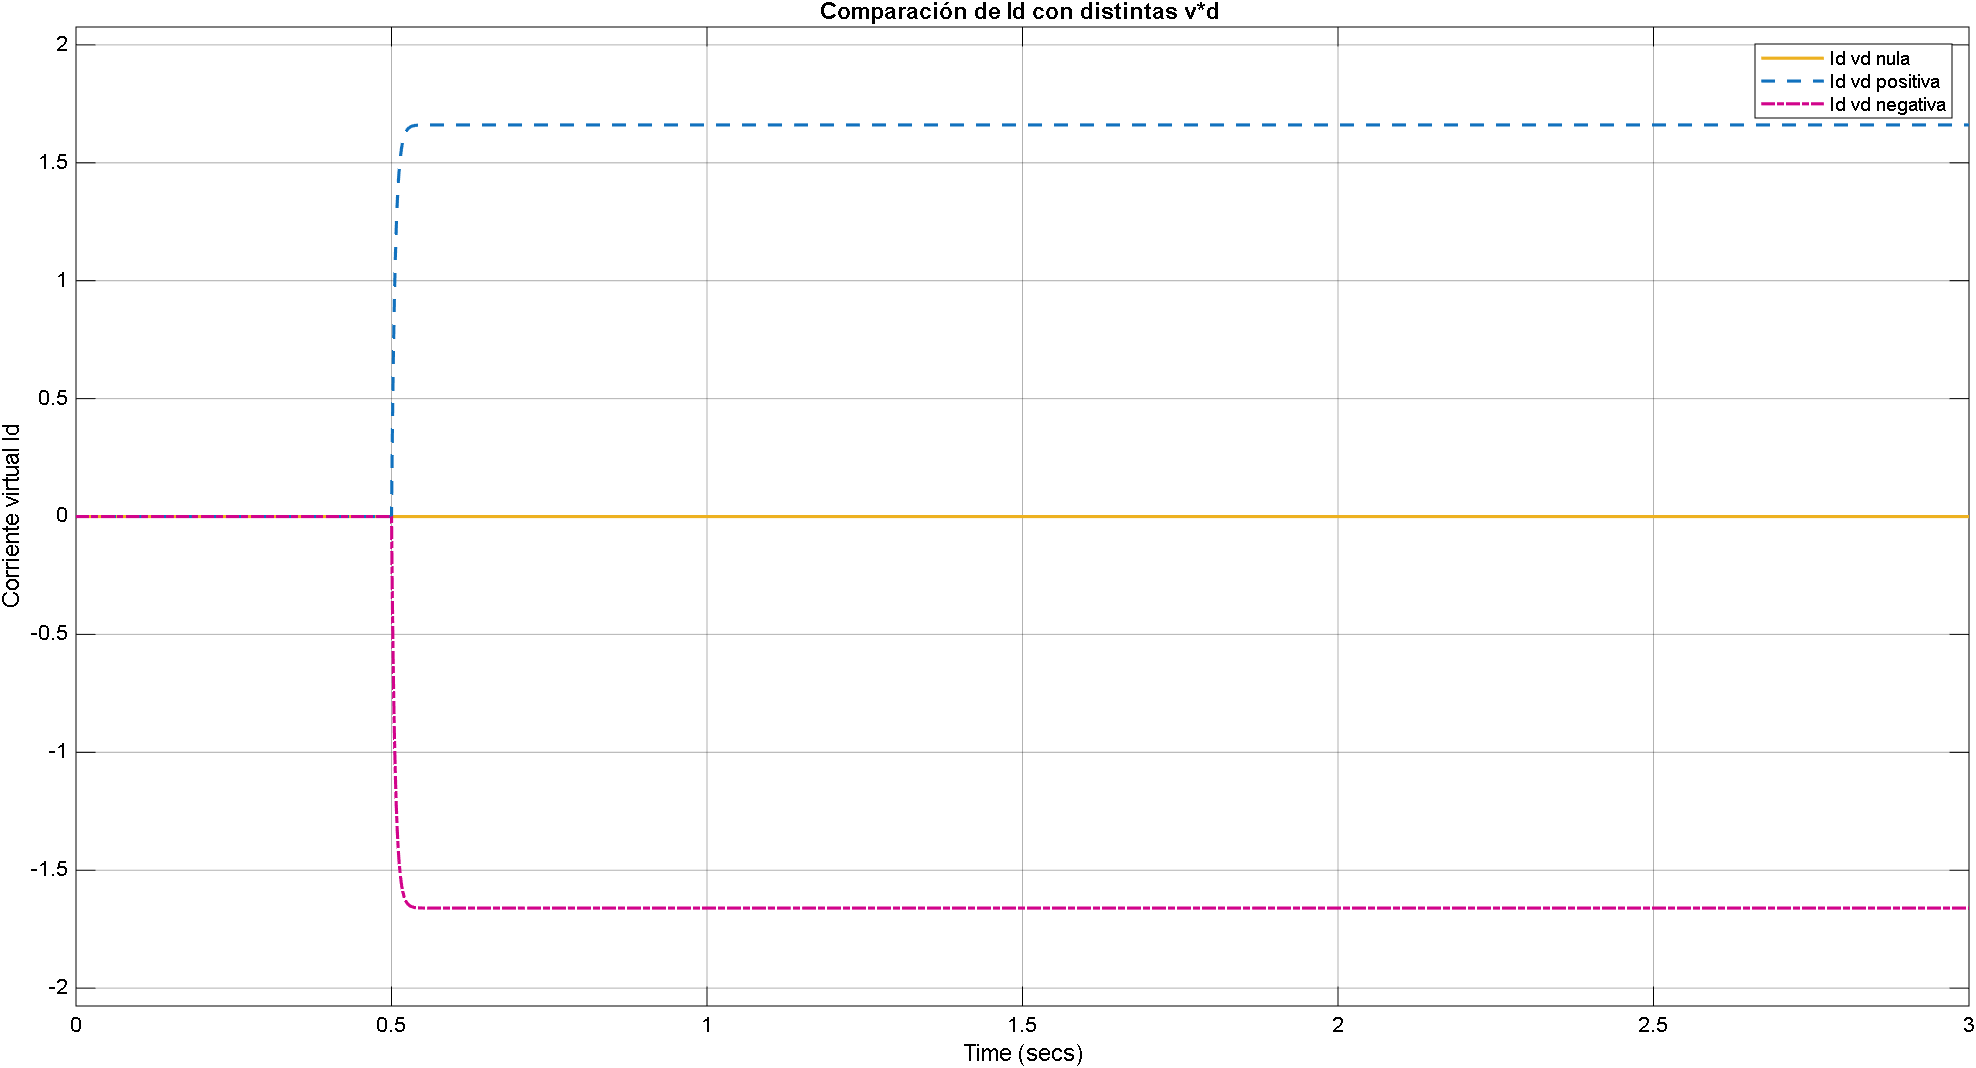
\includegraphics[width=0.86\linewidth,height=0.40\textheight,keepaspectratio]{attachments/Compa_consigna_vd_Id.png}
    \caption{Comparación del comportamiento de la corriente virtual Id con las distintas consignas de $v_{ds}^{r*}$ en el modelo LTI equivalente aumentad}
    \label{fig:comparacion Id con consigna vd LTI}
\end{figure}
Como el sistema LTI equivalente aumentado está desacoplado del eje $d$ las únicas variaciones que se han encontrado fueron en la corriente virtual $i_{ds}^r$,  y por consecuencia en la Temperatura del Estator, que depende del cuadrado de las corrientes virtuales $i_{ds}^r$ y $i_{qs}^r$.

\FloatBarrier
\paragraph{Modelo NL con ley complementaria}
Ahora se verás las gráficas del comportamiento de las variables del Modelo NL con ley complementaria.
\begin{figure}[!htbp]
    \centering
    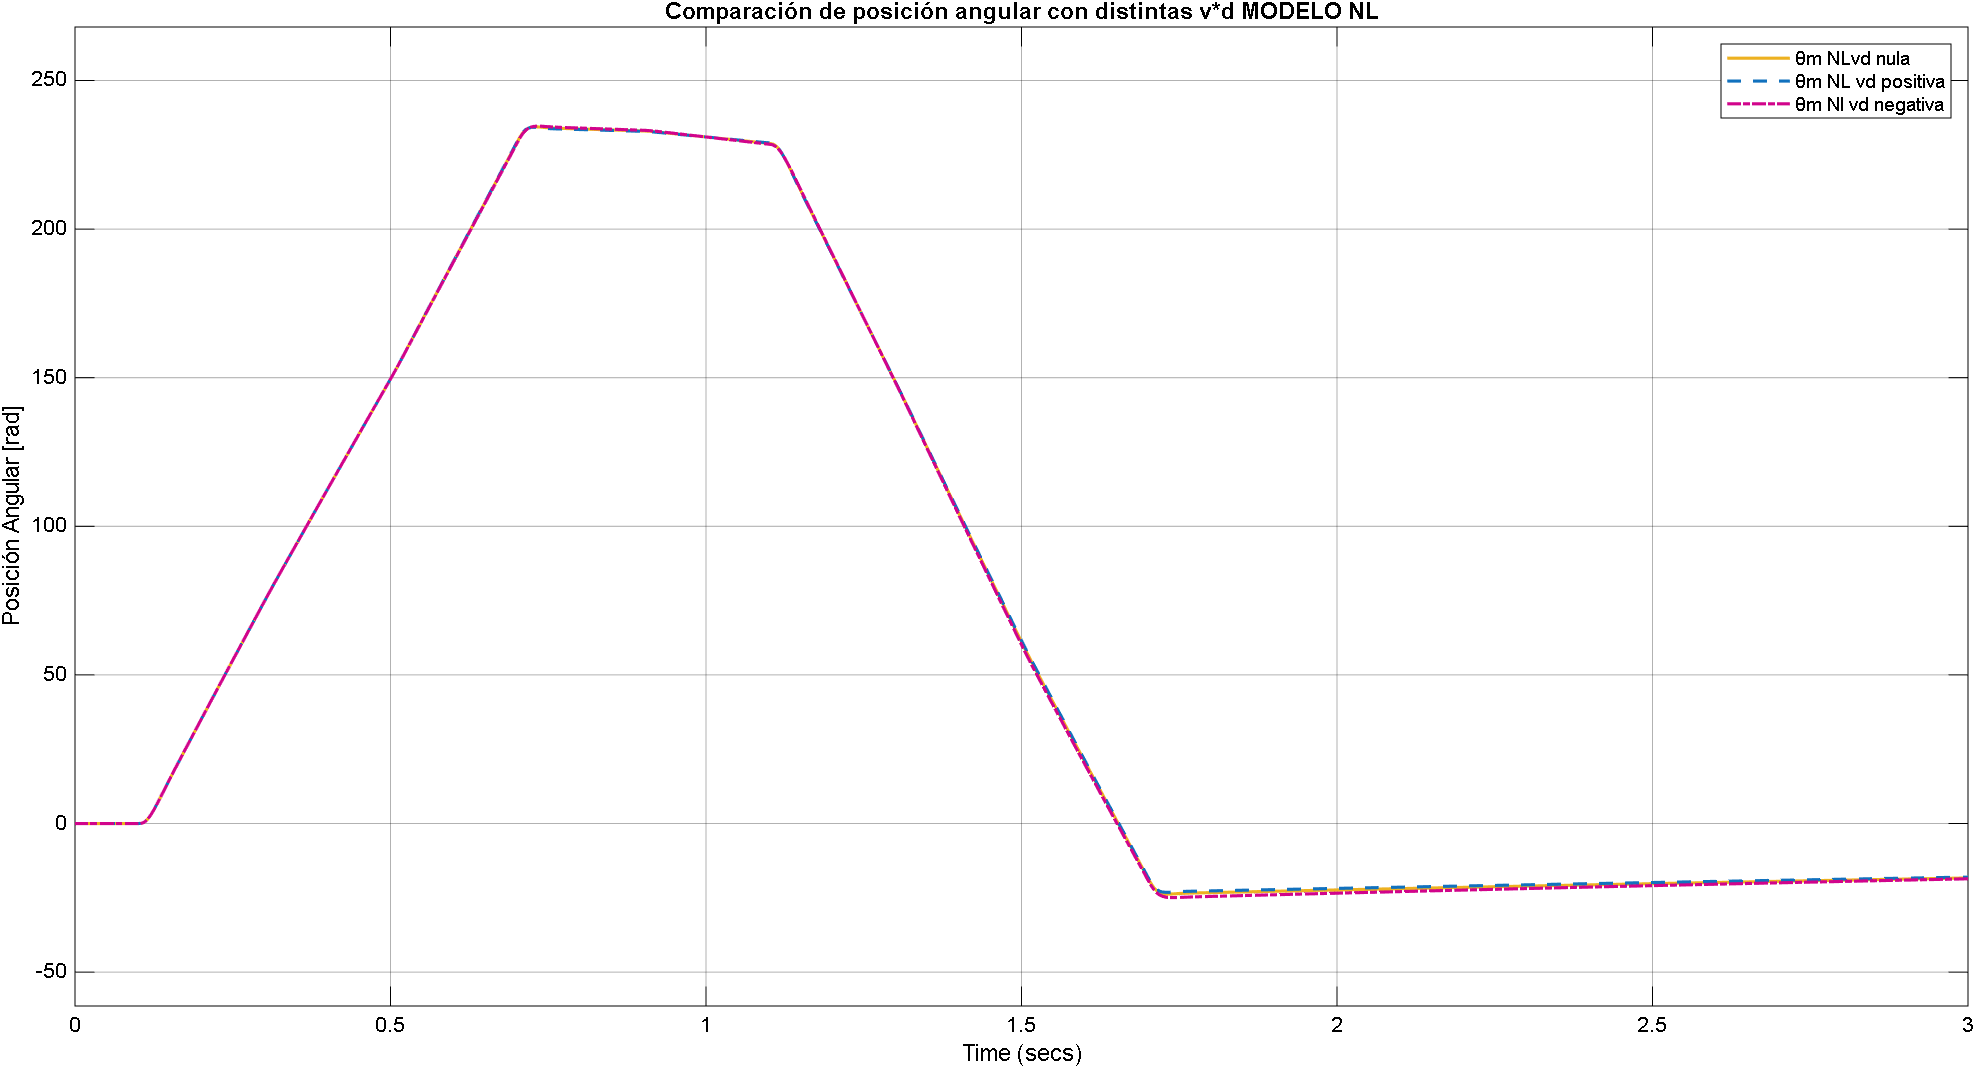
\includegraphics[width=0.86\linewidth,height=0.40\textheight,keepaspectratio]{attachments/Compa_consigna_vd_posici_ang_MODELO NL.png}
    \caption{Comparación del comportamiento de la posición angular con las distintas consignas de $v_{ds}^{r*}$ en el modelo NL con ley complementaria}
    \label{fig:comparacion posicion ang con consigna vd NL}
\end{figure}
\begin{figure}[!htbp]
    \centering
    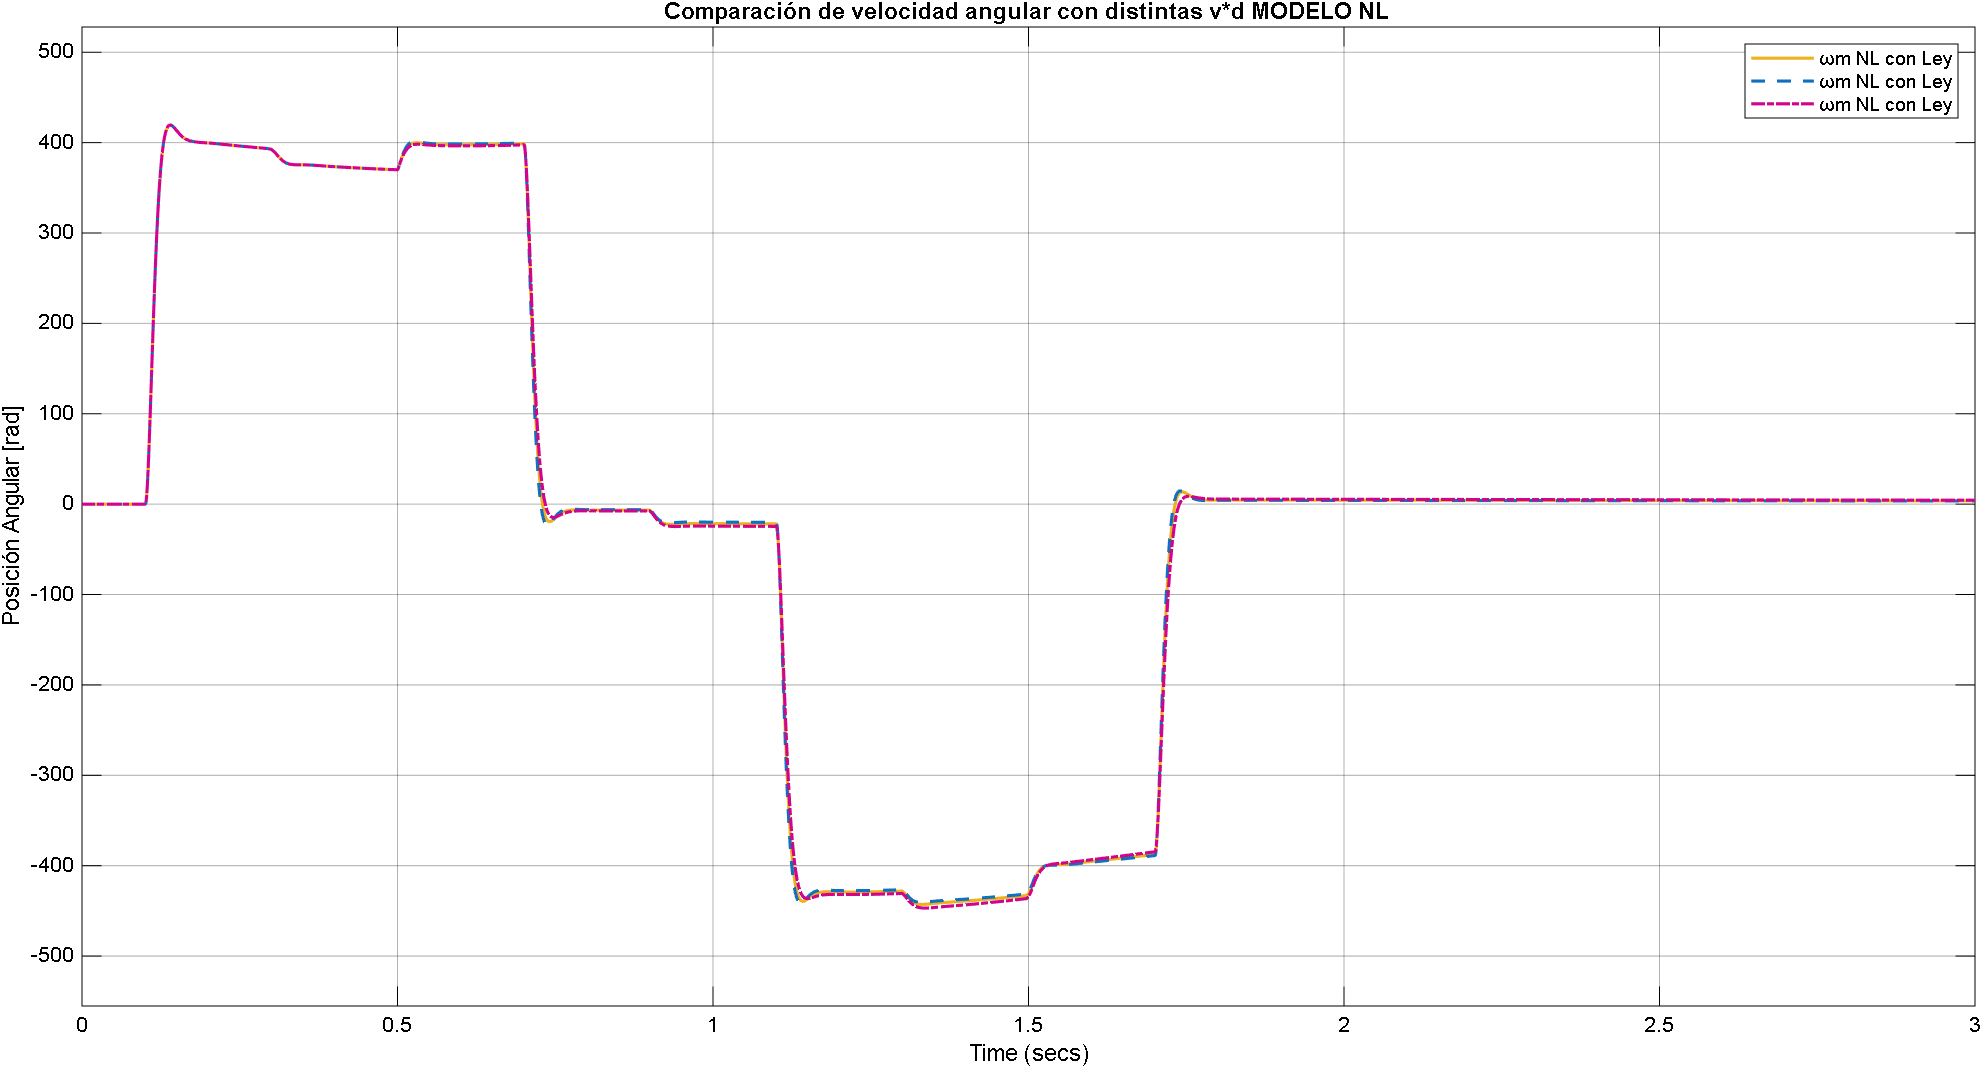
\includegraphics[width=0.86\linewidth,height=0.40\textheight,keepaspectratio]{attachments/Compa_consigna_vd_velocidad_ang_MODELO NL.png}
    \caption{Comparación del comportamiento de la velocidad angular con las distintas consignas de $v_{ds}^{r*}$ en el modelo NL con ley complementaria}
    \label{fig:comparacion velocidad ang con consigna vd NL}
\end{figure}
\begin{figure}[!htbp]
    \centering
    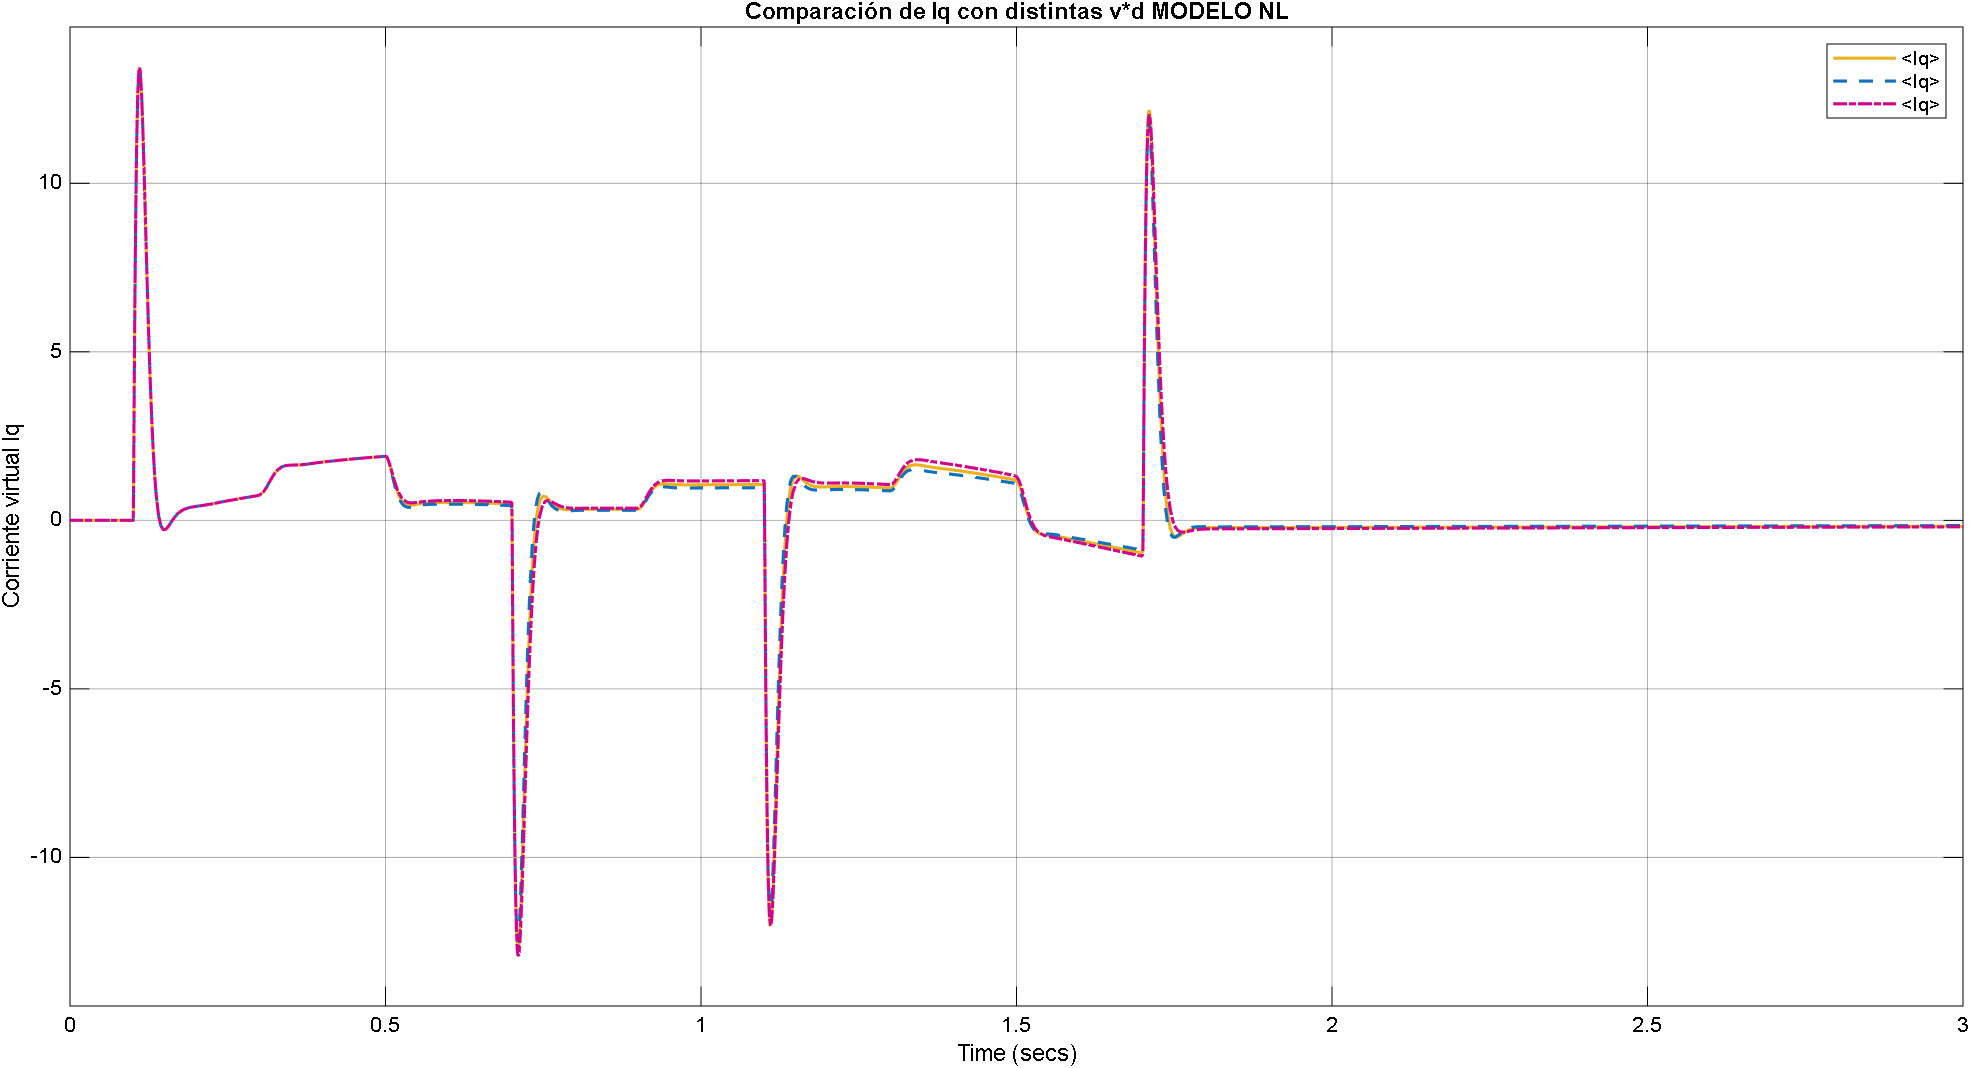
\includegraphics[width=0.86\linewidth,height=0.40\textheight,keepaspectratio]{attachments/Compa_consigna_vd_Iq_MODELO NL.png}
    \caption{Comparación del comportamiento de la corriente virtual Iq con las distintas consignas de $v_{ds}^{r*}$ en el modelo NL con ley complementaria}
    \label{fig:comparacion Iq con consigna vd NL}
\end{figure}
\begin{figure}[!htbp]
    \centering
    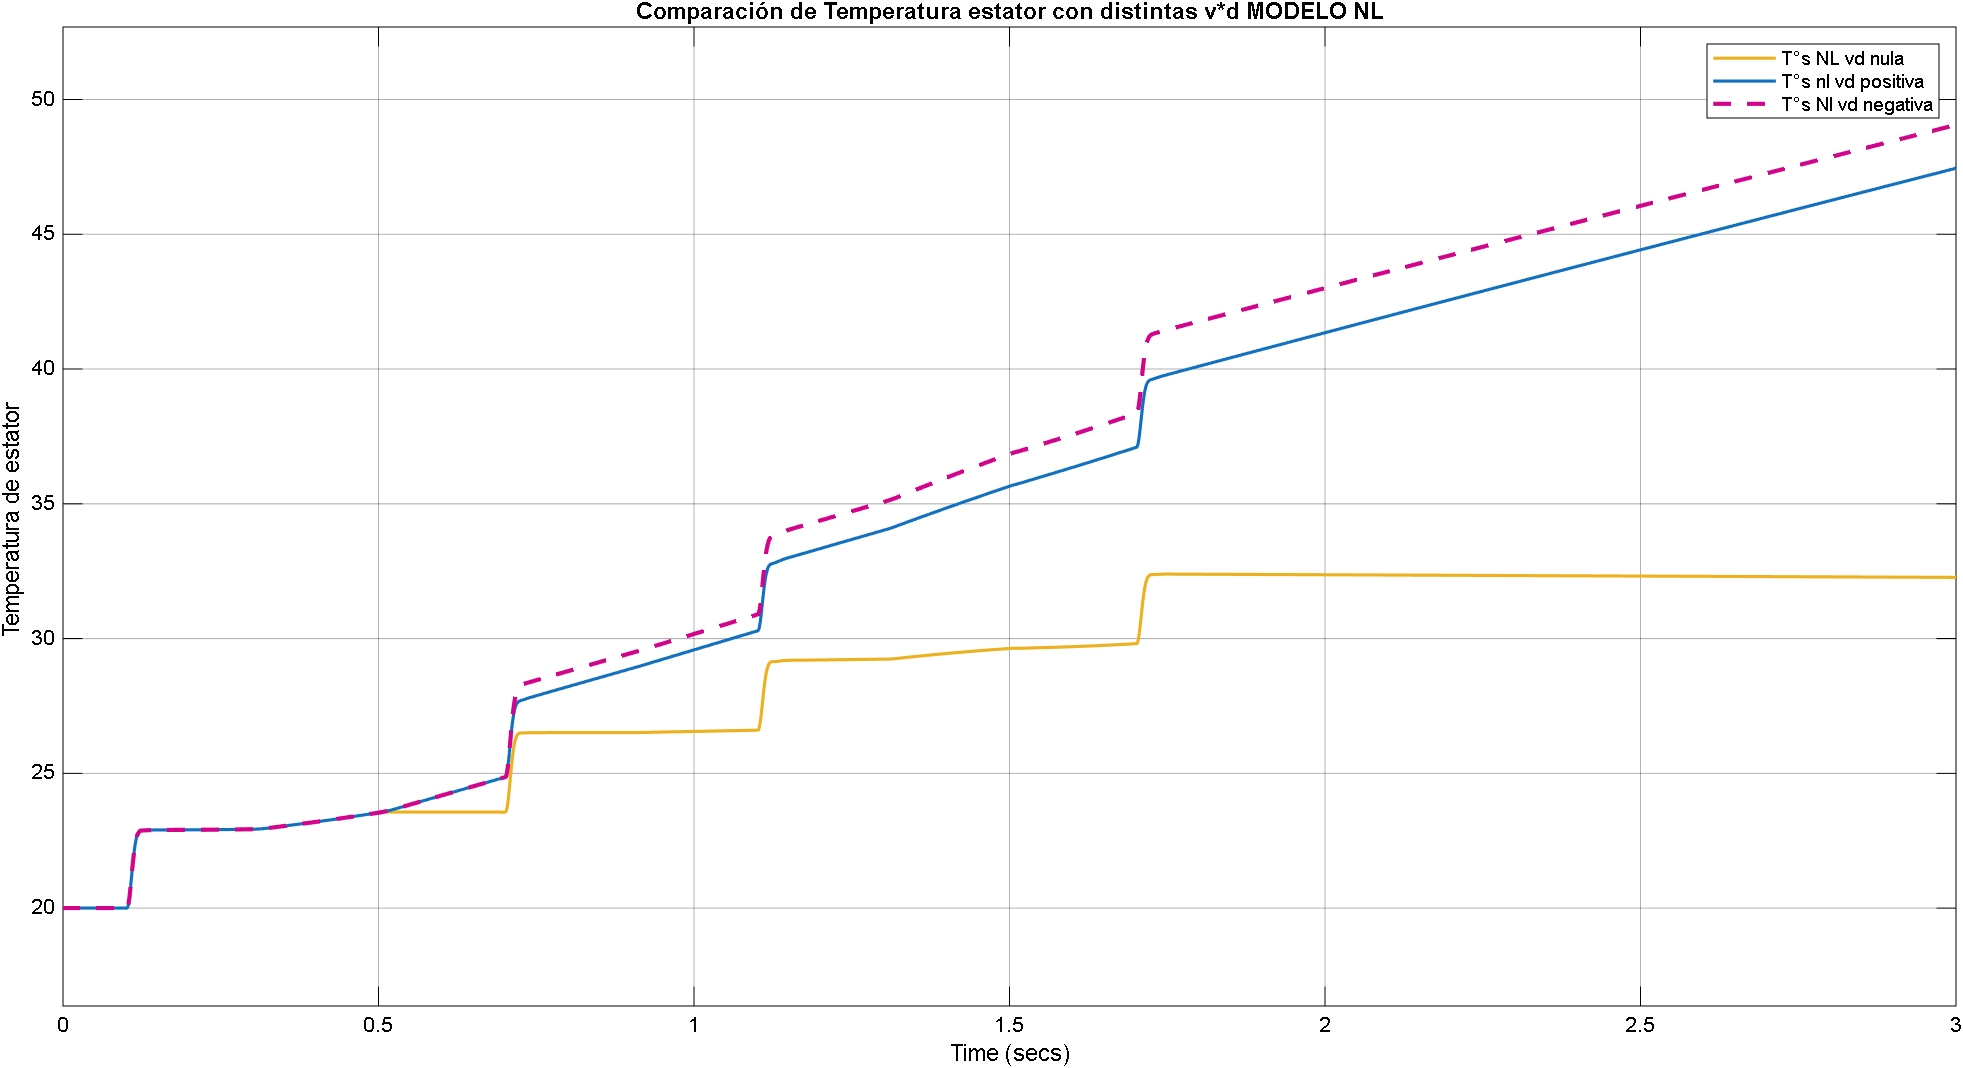
\includegraphics[width=0.86\linewidth,height=0.40\textheight,keepaspectratio]{attachments/Compa_consigna_vd_tempe_estator_MODELO NL.png}
    \caption{Comparación del comportamiento de la temperatura del estator con las distintas consignas de $v_{ds}^{r*}$ en el modelo NL con ley complementaria}
    \label{fig:comparacion tempe estator con consigna vd NL}
\end{figure}
\begin{figure}[!htbp]
    \centering
    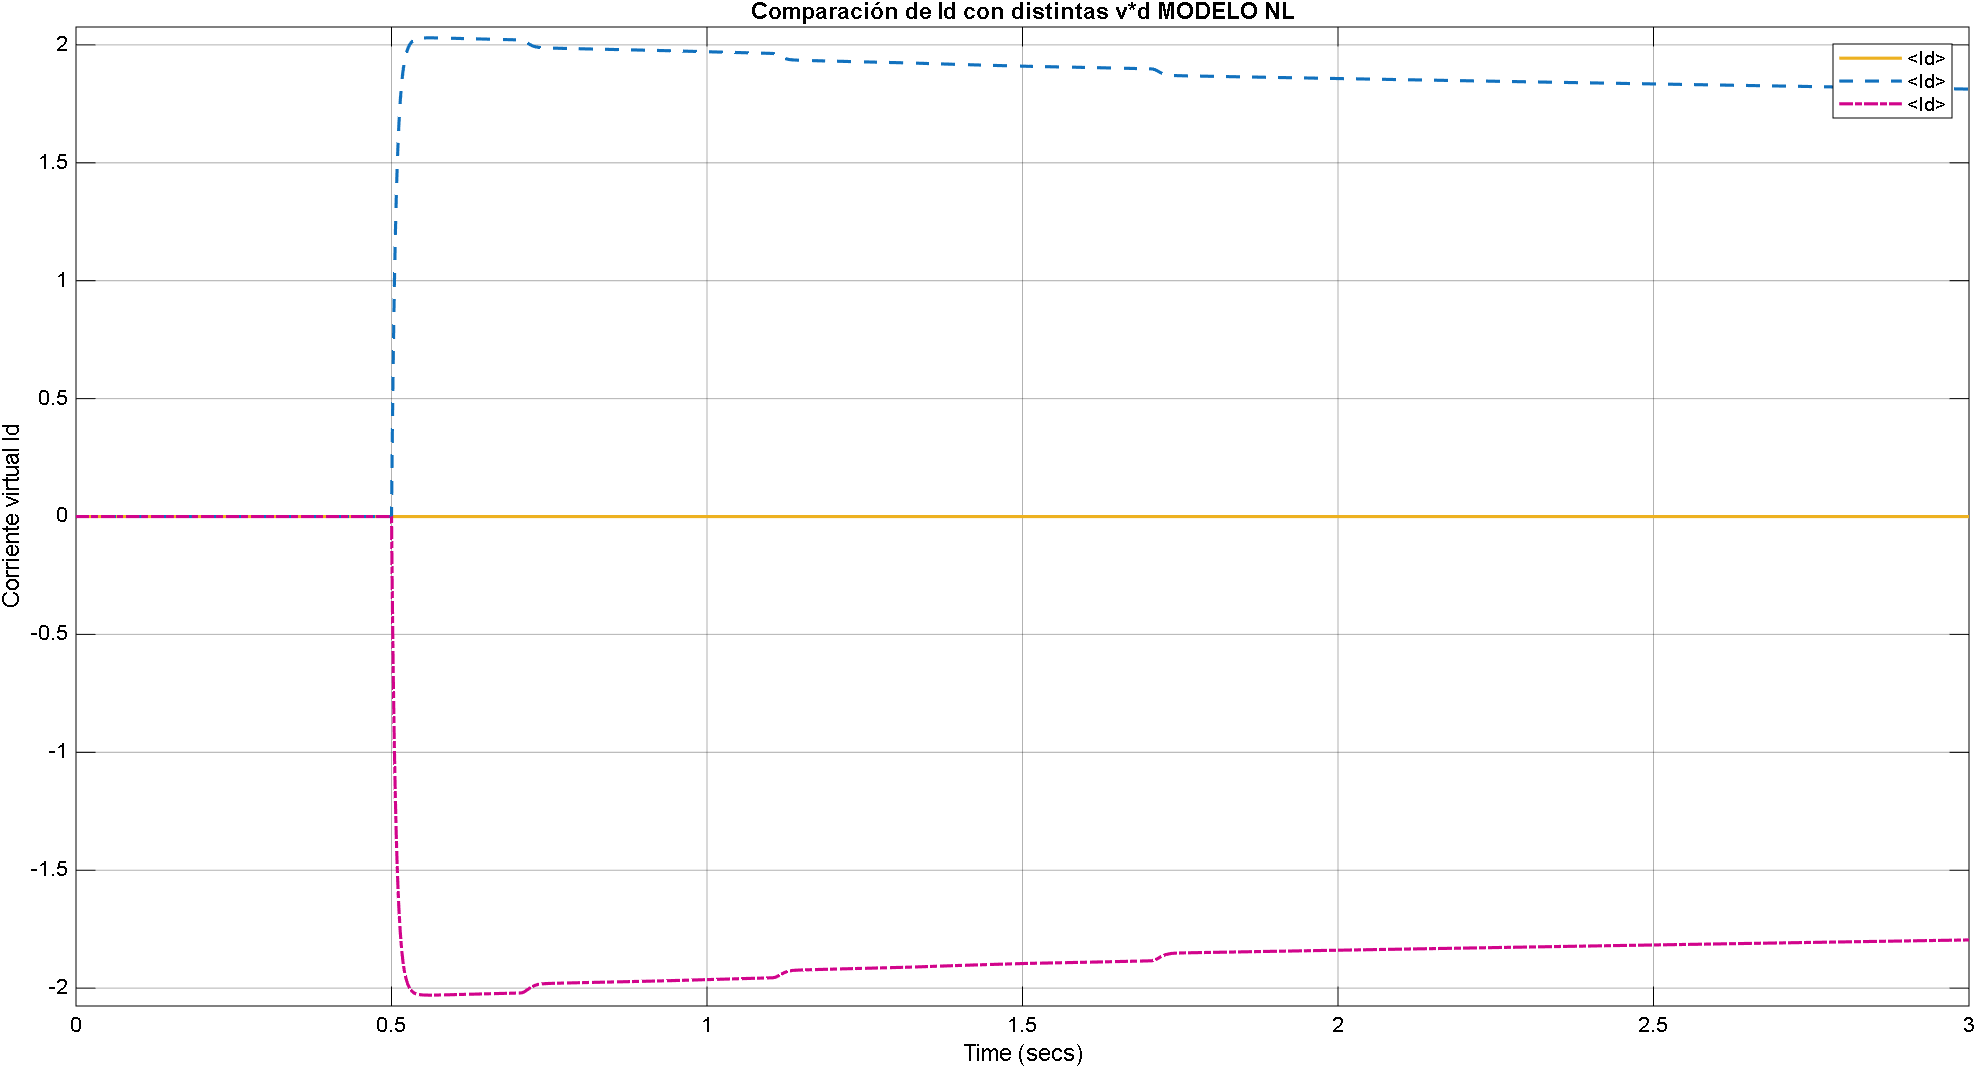
\includegraphics[width=0.86\linewidth,height=0.40\textheight,keepaspectratio]{attachments/Compa_consigna_vd_Id_MODELO NL.png}
    \caption{Comparación del comportamiento de la corriente virtual Id con las distintas consignas de $v_{ds}^{r*}$ en el modelo NL con ley complementaria}
    \label{fig:comparacion Id con consigna vd NL}
\end{figure}
\begin{figure}[!htbp]
    \centering
    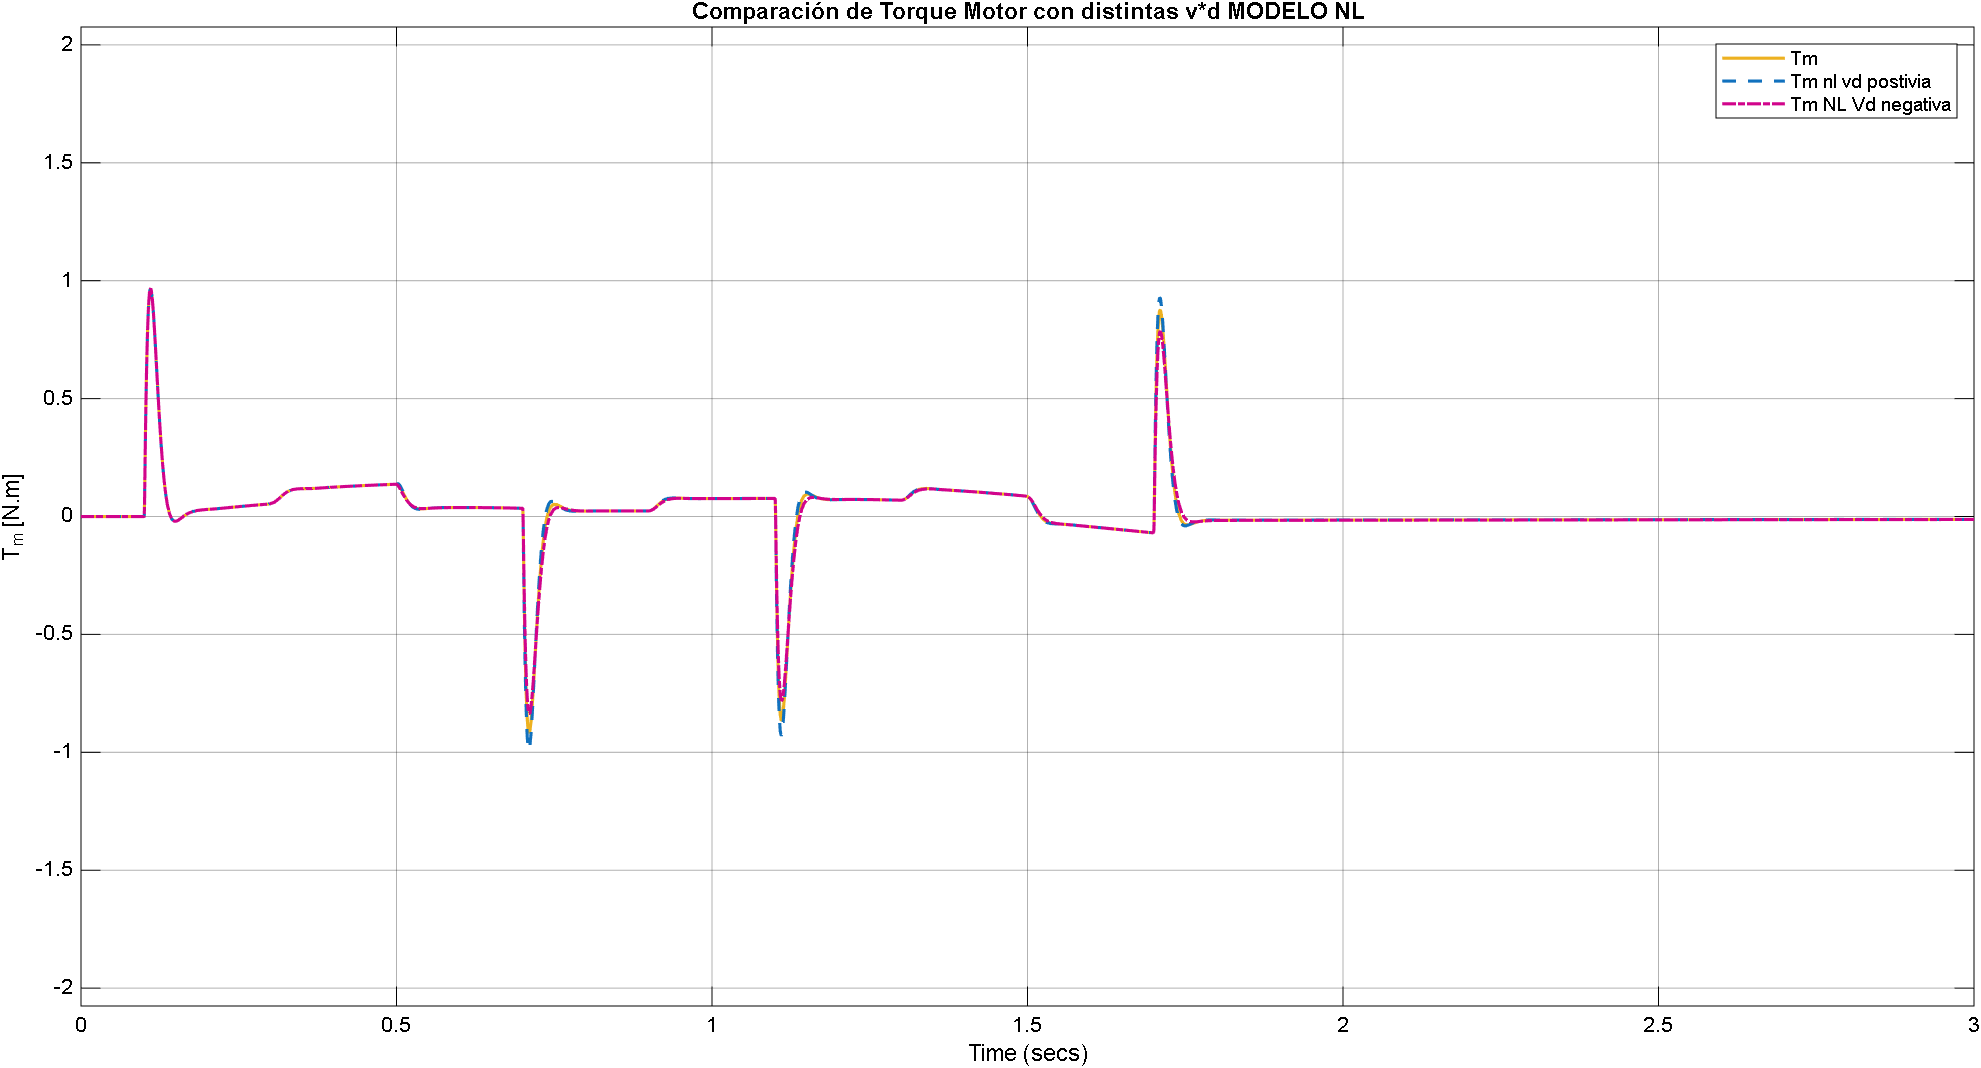
\includegraphics[width=0.86\linewidth,height=0.40\textheight,keepaspectratio]{attachments/Compa_consigna_vd_torque_motor_MODELO NL.png}
    \caption{Comparación del comportamiento del Torque Motor con las distintas consignas de $v_{ds}^{r*}$ en el modelo NL con ley complementaria}
    \label{fig:comparacion Tm con consigna vd NL}
    \par\medskip
    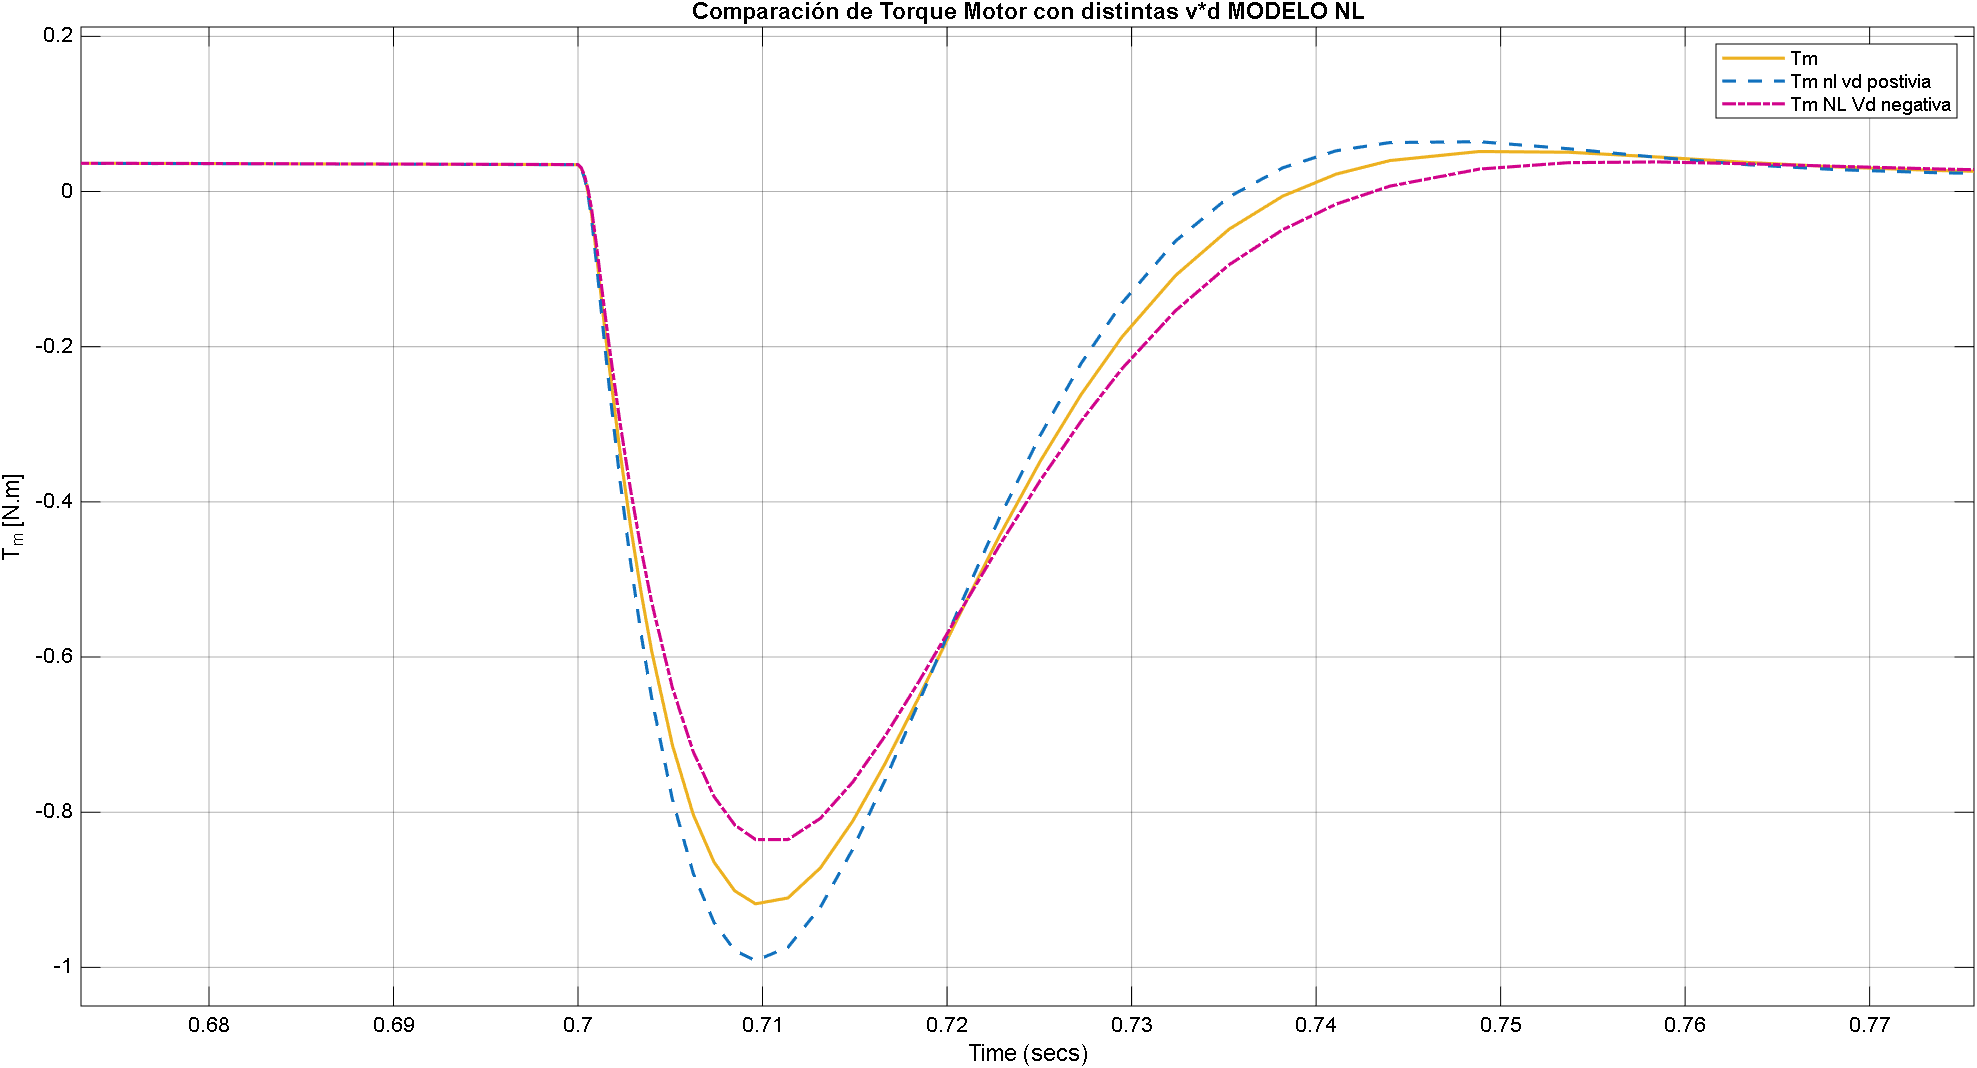
\includegraphics[width=0.86\linewidth,height=0.40\textheight,keepaspectratio]{attachments/Compa_consigna_vd_torque_motor_MODELO NL_DETALLE.png}
    \caption{DETALLE: Comparación del comportamiento del Torque Motor con las distintas consignas de $v_{ds}^{r*}$ en el modelo NL con ley complementaria}
    \label{fig:comparacion Tm con consigna vd NL DETALLE}
\end{figure}

\clearpage
Es posible ver que la aplicación de una consigna de tensión $v_{ds}^r$ modifica la dinámica del accionamiento al alterar el flujo magnético interno de la máquina. Hay 2 casos que son:
\begin{itemize}
    \item Field forcing $(v^r_{ds}>0)$

    El flujo aumenta y el motor desarrolla un torque levemente mayor, generando una repuesta algo más rápida pero con mayores transitorios.

    \item Field weakening $(v^r_{ds}<0)$

    El flujo disminuye, reduciendo el torque disponible y produciendo una respuesta más amortiguada, aunque permitiendo alcanzar velocidades ligeramente superiores.
\end{itemize}
El calentamiento del estator depende tanto del módulo como del signo de la consigna en el eje directo. En debilitamiento de campo ($v_{ds}^{r*} < 0$) la temperatura crece más que en reforzamiento ($v_{ds}^{r*} > 0$), ya que al reducirse el torque disponible el motor exige una mayor corriente $i_{qs}^r$ para sostener la carga, incrementando las pérdidas por efecto Joule en el bobinado.
% ============================================================================= %
% [Start 10/11/2026]
\clearpage
\section{Diseño, análisis y simulación con controlador de movimiento en
cascada con modulador de torque equivalente (control vectorial)}

En la sección anterior se estudió la planta a lazo abierto mediante los modelos LPV y LTI equivalente, y se analizaron sus propiedades de estabilidad, controlabilidad y observabilidad. A continuación, se aborda el diseño de una estrategia de control a lazo cerrado basada en el \textbf{control en cascada}. Esta estructura aprovecha la diferencia entre las constantes de tiempo de los subsistemas eléctrico y mecánico para organizar el control en lazos con distintas velocidades de respuesta.

La estrategia se organiza en dos lazos principales:

\begin{itemize}
    \item \textbf{Lazo interno (rápido):} Controla la dinámica eléctrica de la máquina, regulando las corrientes y, por consiguiente, el torque electromagnético. Su respuesta debe ser más rápida que la del lazo externo.
    \item \textbf{Lazo externo (lento):} Controla la dinámica mecánica del accionamiento para satisfacer las consignas de posición y velocidad frente a los requerimientos de la carga.
\end{itemize}
    
Para implementar esta estrategia, el sistema de control se estructura en los siguientes bloques funcionales:

\begin{itemize}
    \item \textbf{Modulador de torque equivalente (lazo interno):} Vincula la consigna de torque con las variables eléctricas de la máquina. Mediante la generación de referencias de corriente, su regulación y la compensación de los acoplamientos, determina las tensiones necesarias en los ejes rotativos para alcanzar el torque solicitado.
    \item \textbf{Controlador de movimiento (lazo externo):} Emplea un esquema PID que recibe las consignas de movimiento y genera la referencia de torque a partir de los errores de seguimiento.
    \item \textbf{Observador de estado de orden reducido:} Estima las variables mecánicas no medidas, como la velocidad del rotor, a partir de la posición medida y del modelo del sistema. De esta manera, proporciona la información necesaria para la realimentación sin recurrir a la derivación directa de la señal de posición, sensible al ruido de medición.
\end{itemize}




% ======================================================================================================================================================================================%
\subsection{Modulador de torque equivalente}
El modulador de torque equivalente recibe una consigna de torque y calcula las tensiones que deben aplicarse a la máquina para producirlo. Su diseño combina la compensación de las realimentaciones naturales de la planta con la regulación de las corrientes virtuales.

El desarrollo se divide en tres etapas:
\begin{itemize}
    \item Modulación de tensiones y desacoplamiento por realimentación no lineal.
    \item Diseño de los lazos de control de corrientes virtuales con desacoplamiento mutuo y respecto de la velocidad angular.
    \item Compensación del torque de carga por gravedad.
\end{itemize}

En conjunto, estas etapas permiten pasar de la consigna de torque a las referencias de corriente y, a partir de ellas, a las tensiones virtuales que se aplican a la planta global no lineal.

% Realizar gráfico:

% Consigna Torque ->_{define} Consigna Corriente Virtual Q ->_{define} Consigna de Tensiones Virtuales dq0 ->_{obtiene} Tensiones Virtuales dq0 a aplicar a la planta Global No Lineal. 

% ======================================================================================================================================================================================%
\subsubsection{Modulación de tensiones y desacoplamiento por realimentación no lineal}

Las tensiones virtuales $v_{ds}^{r}(t)$, $v_{qs}^{r}(t)$ y $v_{0s}^{r}(t)$ son las entradas de control del subsistema electromagnético y actúan directamente sobre la dinámica de las corrientes virtuales. Estas corrientes determinan el torque electromagnético que, a su vez, modifica la velocidad y la posición angular del accionamiento. Por lo tanto, el diseño comienza por las ecuaciones de las corrientes:

\begin{equation}
\label{eq:dinamica-corrientes}
\begin{aligned}
\frac{di_{ds}^{r}(t)}{dt} & = \frac{1}{L_{d}} \left[ v_{ds}^{r}(t) - R_{s} \Big( T_{s}^{\circ} (t) \Big) i_{ds}^{r}(t) + L_{q}i_{qs}^{r}(t) \omega_{m}(t)P_{p}  \right]  \\
\frac{di_{qs}^{r}(t)}{dt}  & = \frac{1}{L_{q} } \left[ v_{qs}^{r}(t) - R_{s} \Big( T_{s}^{\circ} (t) \Big) i_{qs}^{r}(t) - \big[ \lambda_{m}^{'r} + L_{d} i_{ds}^{r}(t) \big] \omega_{m}(t)P_{p} \right]  \\
\frac{di_{0s}^{r}(t)}{dt} & = \frac{1}{ L_{ls} } \left[ v_{0s}^{r}(t) - R_{s} \Big( T_{s}^{\circ} (t) \Big) i_{0s}^{r}(t) \right]
\end{aligned}
\end{equation}

Para compensar las caídas resistivas y los términos de acoplamiento y fuerza contraelectromotriz, se proponen las siguientes tensiones virtuales:
\begin{align}
v_{ds}^{r}(t) & = v_{ds}^{*r}(t) + R_{s} \Big( T_{s}^{\circ} (t) \Big) i_{ds}^{r}(t) - L_{q}i_{qs}^{r}(t) \omega_{m}(t)P_{p}
\label{eq:compensacion-tension-d} \\
v_{qs}^{r}(t) & = v_{qs}^{*r}(t) + R_{s} \Big( T_{s}^{\circ} (t) \Big) i_{qs}^{r}(t) + \big[ \lambda_{m}^{'r} + L_{d} i_{ds}^{r}(t) \big] \omega_{m}(t)P_{p}
\label{eq:compensacion-tension-q} \\
v_{0s}^{r}(t) & = v_{0s}^{*r}(t) + R_{s} \Big( T_{s}^{\circ} (t) \Big) i_{0s}^{r}(t)
\label{eq:compensacion-tension-cero}
\end{align}

\noindent Se define así:
\begin{description}[
    leftmargin=2.5cm,
    labelwidth=2cm,
    labelsep=0.5cm,
    align=left,
    font=\normalfont
]
    \item[$v_{ds}^{*r}(t)$] Consigna de tensión del eje directo.
    \item[$v_{qs}^{*r}(t)$] Consigna de tensión del eje en cuadratura.
    \item[$v_{0s}^{*r}(t)$] Consigna de tensión del eje cero.
\end{description}

Al sustituir estos valores de $v_{ds}^{r}(t)$, $v_{qs}^{r}(t)$ y $v_{0s}^{r}(t)$ en las ecuaciones dinámicas de las corrientes \eqref{eq:dinamica-corrientes}, se obtiene:

\begin{align*}
\frac{di_{ds}^{r}(t)}{dt} & = \frac{1}{L_{d}} \Bigg[ \Big( v_{ds}^{*r}(t) + \cancel{ R_{s} \Big( T_{s}^{\circ} (t) \Big) i_{ds}^{r}(t) } - \cancel{ L_{q}i_{qs}^{r}(t) \omega_{m}(t)P_{p} } \Big) - \cancel{ R_{s} \Big( T_{s}^{\circ} (t) \Big) i_{ds}^{r}(t) } + \cancel{ L_{q}i_{qs}^{r}(t) \omega_{m}(t)P_{p}  } \Bigg]  \\
\frac{di_{qs}^{r}(t)}{dt}  & = \frac{1}{L_{q} } \Bigg[ \Big( v_{qs}^{*r}(t) +\cancel{  R_{s} \Big( T_{s}^{\circ} (t) \Big) i_{qs}^{r}(t) } +\cancel{  \big[ \lambda_{m}^{'r} + L_{d} i_{ds}^{r}(t) \big] \omega_{m}(t)P_{p}  } \Big) - \cancel{ R_{s} \Big( T_{s}^{\circ} (t) \Big) i_{qs}^{r}(t) } - \cancel{ \big[ \lambda_{m}^{'r} + L_{d} i_{ds}^{r}(t) \big] \omega_{m}(t)P_{p}  }\Bigg]  \\
\frac{di_{0s}^{r}(t)}{dt} & = \frac{1}{ L_{ls} } \Bigg[ \Big( v_{0s}^{*r}(t) + \cancel{ R_{s} \Big( T_{s}^{\circ} (t) \Big) i_{0s}^{r}(t) }  \Big) -\cancel{  R_{s} \Big( T_{s}^{\circ} (t) \Big) i_{0s}^{r}(t) } \Bigg]
\end{align*}

Con las compensaciones \eqref{eq:compensacion-tension-d}--\eqref{eq:compensacion-tension-cero}, las dinámicas de las corrientes virtuales se simplifican a:
\begin{align}
\frac{di_{ds}^{r}(t)}{dt} & = \frac{1}{L_{d}} v_{ds}^{*r}(t)
\label{eq:corriente-desacoplada-d} \\
\frac{di_{qs}^{r}(t)}{dt}  & = \frac{1}{L_{q} } v_{qs}^{*r}(t)
\label{eq:corriente-desacoplada-q} \\
\frac{di_{0s}^{r}(t)}{dt} & = \frac{1}{ L_{ls} } v_{0s}^{*r}(t)
\label{eq:corriente-desacoplada-cero}
\end{align}

\clearpage

\begin{figure}[!htbp]
    \centering
    \begin{adjustbox}{max totalsize={\linewidth}{0.65\textheight},center}
        \begin{minipage}{\linewidth}
            \centering
            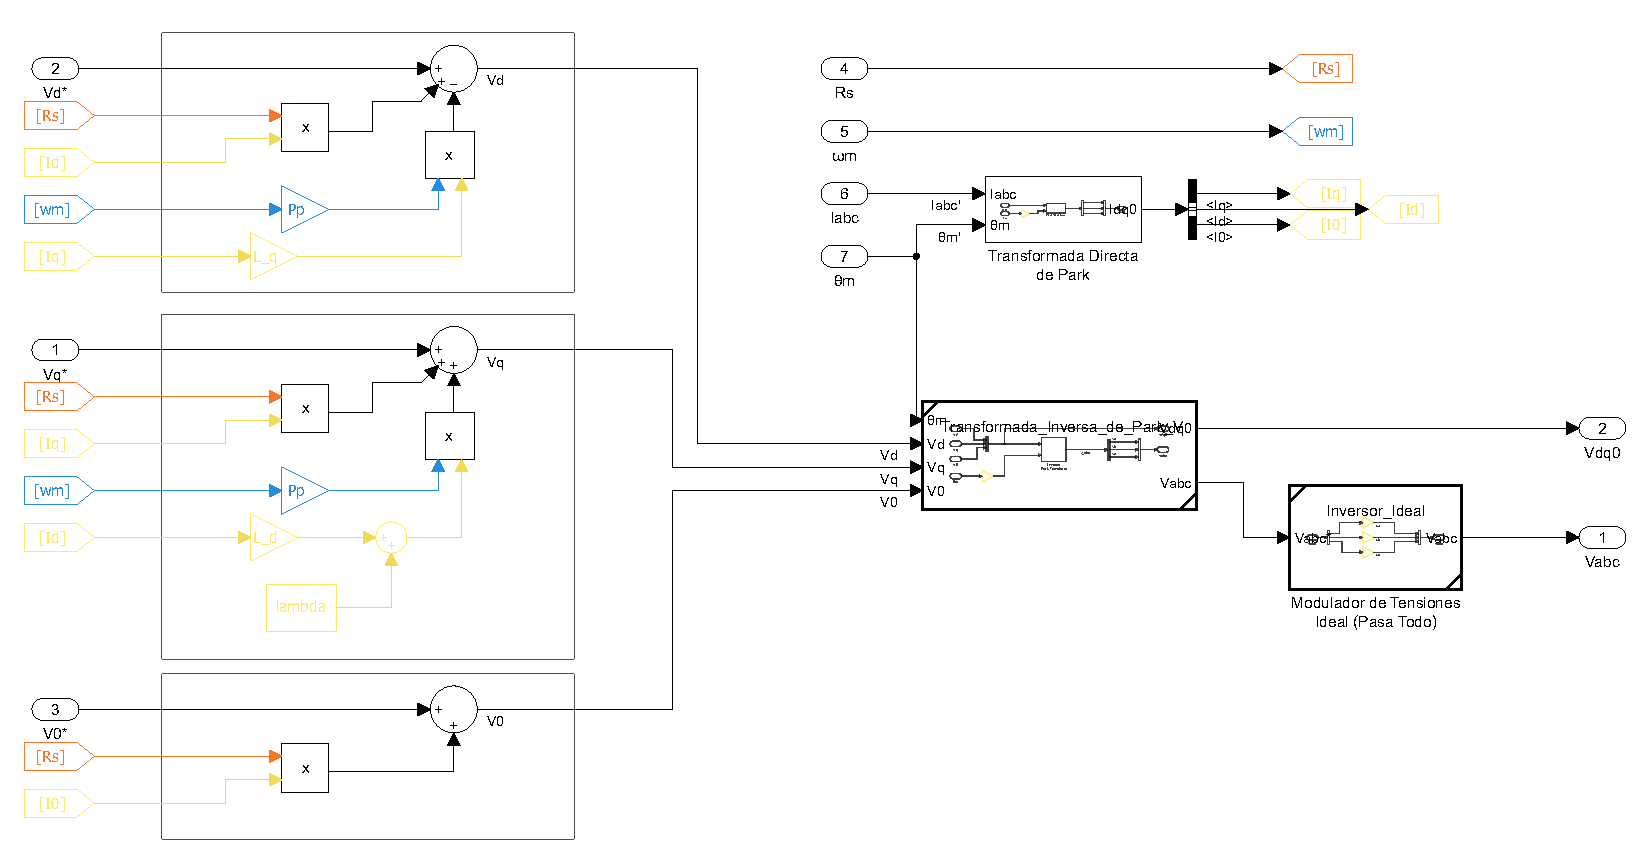
\includegraphics[width=\linewidth]{attachments/Modulador de Tensiones Virtuales.pdf}
            \par\vspace{4mm}
            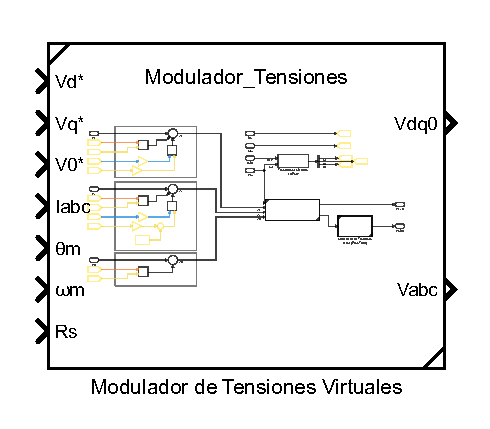
\includegraphics[width=0.42\linewidth,height=0.19\textheight,keepaspectratio]{attachments/Bloque Modulador de Tensiones Virtuales.pdf}
        \end{minipage}
    \end{adjustbox}
    \caption{Bloque de modulación de tensiones virtuales y retroalimentación no lineal}
    \label{fig:ModTensionesVirtuales}
\end{figure}

Se compara el comportamiento del modelo Global No Lineal (GNL)
con Ley de Control Mínima Complementaria y con el Modulador de
Tensión, antes de incorporar los reguladores de corriente.
La diferencia entre ambas estrategias se reconoce en las
ecuaciones de las corrientes virtuales.

Con la Ley de Control Mínima Complementaria, las dinámicas
eléctricas resultan:
\begin{equation}
\left\{
\begin{aligned}
    L_d \frac{di_{ds}^{r}}{dt}
    &= v_{ds}^{*r} - R_s(T_s^\circ)i_{ds}^{r} \\
    L_q \frac{di_{qs}^{r}}{dt}
    &= v_{qs}^{*r} - R_s(T_s^\circ)i_{qs}^{r}
       - \lambda_m^{'r}P_p\omega_m \\
    L_{ls} \frac{di_{0s}^{r}}{dt}
    &= v_{0s}^{*r} - R_s(T_s^\circ)i_{0s}^{r}
\end{aligned}
\right.
\label{eq:corrientes-ley-mc}
\end{equation}
Para la aproximación con resistencia constante, se sustituye
$R_s(T_s^\circ)$ por $R_s^\ell$.

Esta ley elimina los acoplamientos eléctricos no lineales
considerados en su deducción, pero conserva las caídas resistivas
y la fuerza contraelectromotriz debida al movimiento. Por tanto,
la corriente en cuadratura continúa acoplada con la velocidad
angular del motor.

En cambio, el Modulador de Tensión compensa adicionalmente estos
términos. Bajo compensación exacta de parámetros y estados, y con
un inversor ideal, se obtiene:
\begin{equation}
\left\{
\begin{aligned}
    L_d \frac{di_{ds}^{r}}{dt} &= v_{ds}^{*r} \\
    L_q \frac{di_{qs}^{r}}{dt} &= v_{qs}^{*r} \\
    L_{ls} \frac{di_{0s}^{r}}{dt} &= v_{0s}^{*r}
\end{aligned}
\right.
\label{eq:corrientes-modulador-tension}
\end{equation}
Así, cada corriente queda desacoplada de las demás corrientes y
de la velocidad, y su derivada depende únicamente de la tensión
virtual aplicada y de la inductancia correspondiente.

Esta modificación cambia sustancialmente la respuesta a una
misma consigna de tensión. Para una tensión virtual constante
$v_{qs}^{*r}=V_{q,\mathrm{nom}}$, la dinámica ideal compensada
predice una corriente creciente en forma lineal:
\begin{equation}
    \frac{di_{qs}^{r}}{dt}
    = \frac{V_{q,\mathrm{nom}}}{L_q}
    = \frac{19.596}{5.8\times10^{-3}}
    \approx 3379\;\mathrm{\frac{A}{s}}.
\end{equation}
Para $i_{ds}^{r}=0$, el torque electromagnético es proporcional
a $i_{qs}^{r}$, por lo que también crecería linealmente durante
la aplicación de dicha tensión. En contraste, con la Ley de
Control Mínima Complementaria, la caída resistiva y la fuerza
contraelectromotriz limitan el crecimiento de la corriente y,
por consiguiente, del torque.

En los resultados presentados se utiliza el valor constante
$R_s^\ell$ en la compensación del Modulador de Tensión, mientras
que la planta GNL conserva la dependencia $R_s(T_s^\circ)$.
Esta elección responde a las dificultades numéricas observadas
al utilizar la compensación con resistencia dependiente de la
temperatura: las elevadas corrientes producen grandes pérdidas
por efecto Joule, que aceleran la evolución térmica y, por
consiguiente, la variación de la resistencia. En estas condiciones,
la simulación presenta dificultades para completar el cálculo
y obtener las curvas. Por ello, la comparación mostrada se
realiza con resistencia constante en la compensación.

Las Figuras~\ref{fig:tm-leycmc-vs-modtension}
y~\ref{fig:wm-leycmc-vs-modtension} muestran las respuestas
obtenidas en la simulación.

\begin{figure}[!htbp]
    \centering
    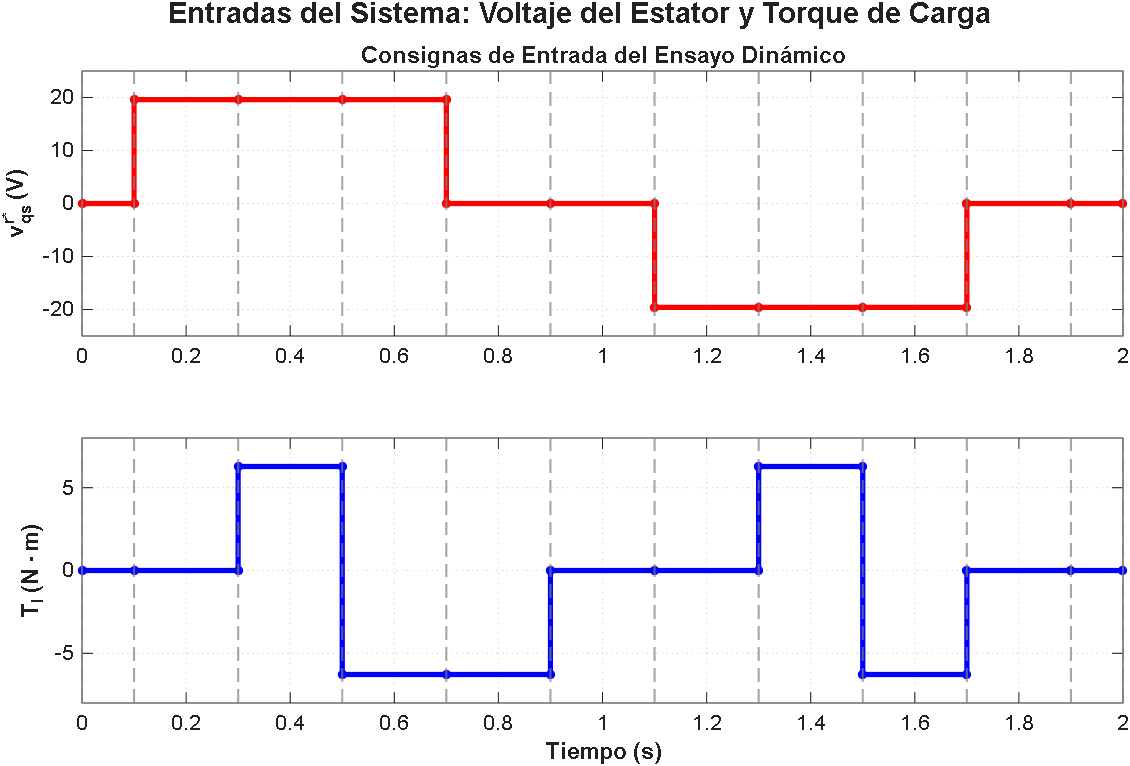
\includegraphics[width=0.84\linewidth]{attachments/VariacionTorqueyTension.png}
    \caption{Perfiles de entrada utilizados en el ensayo dinámico "Comparación del modelo GBL con Ley de Control Minima Complementaria vs Modulador de Tensión": tensión de referencia en el eje en cuadratura $v_{qs}^{*r}(t)$ (arriba) y torque de carga $T_l(t)$ (abajo).}
    \label{fig:entradas-modulador-tension}
\end{figure}

\begin{figure}[!htbp]
    \centering
    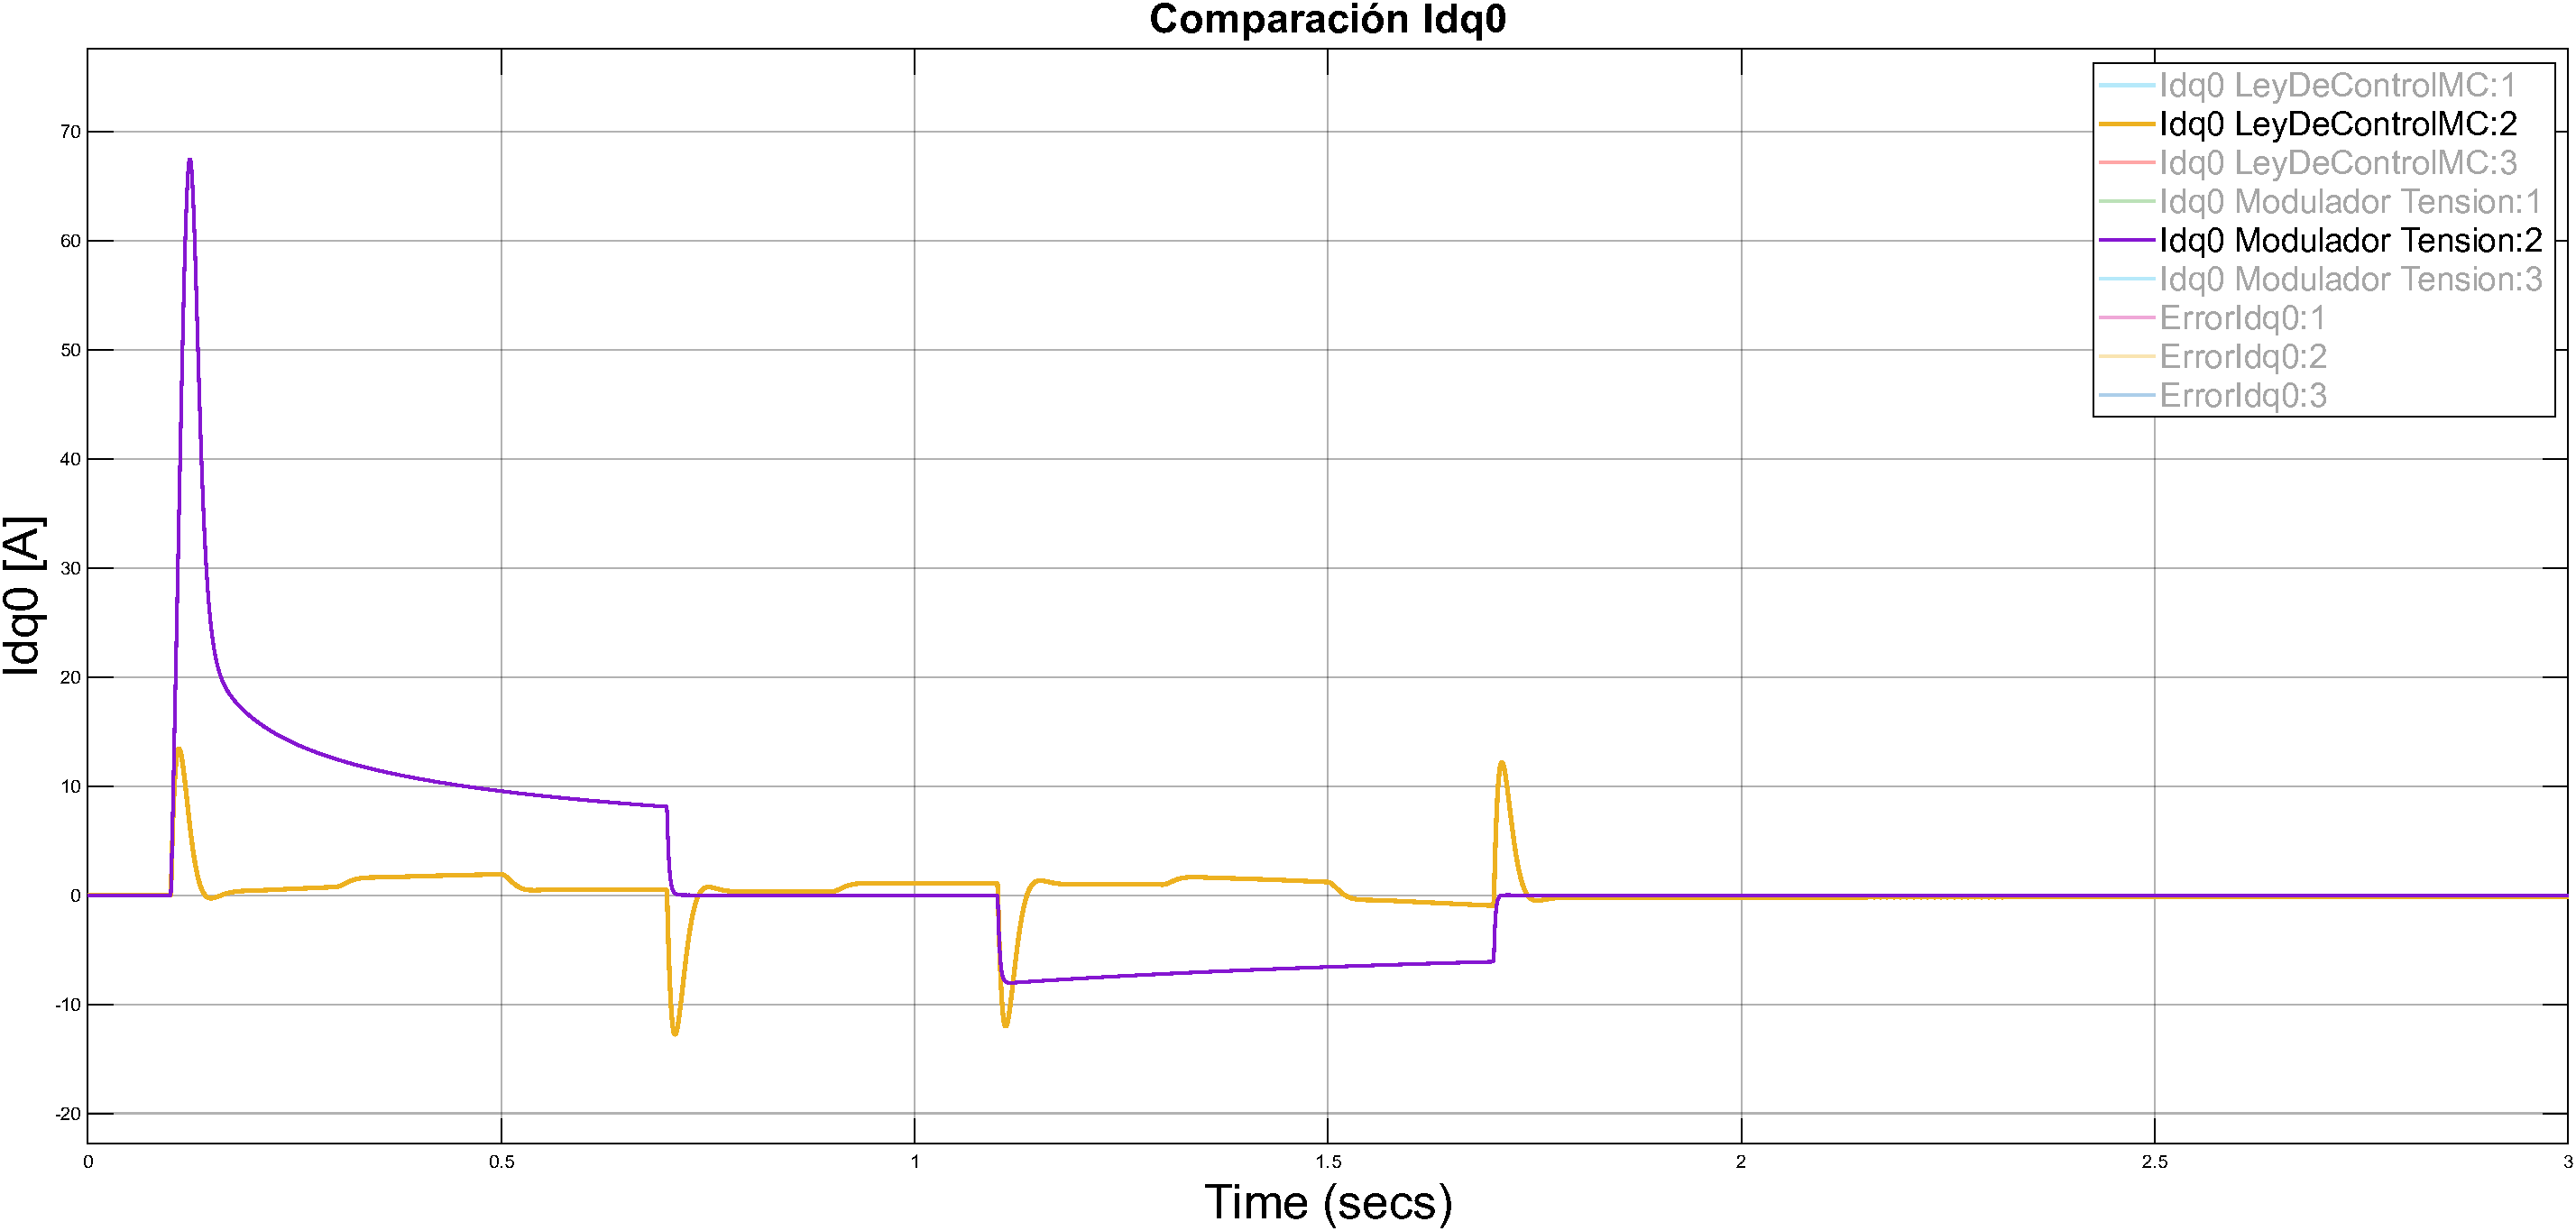
\includegraphics[width=0.95\linewidth]
        {attachments/Iq_LeyCMC_vs_ModTension.pdf}
    \caption{Corrientes virtuales $i_{dq0}$ del modelo GNL con Ley de
    Control Mínima Complementaria y con Modulador de Tensión
    utilizando resistencia constante en la compensación.}
    \label{fig:Iq-leycmc-vs-modtension}
\end{figure}

\begin{figure}[!htbp]
    \centering
    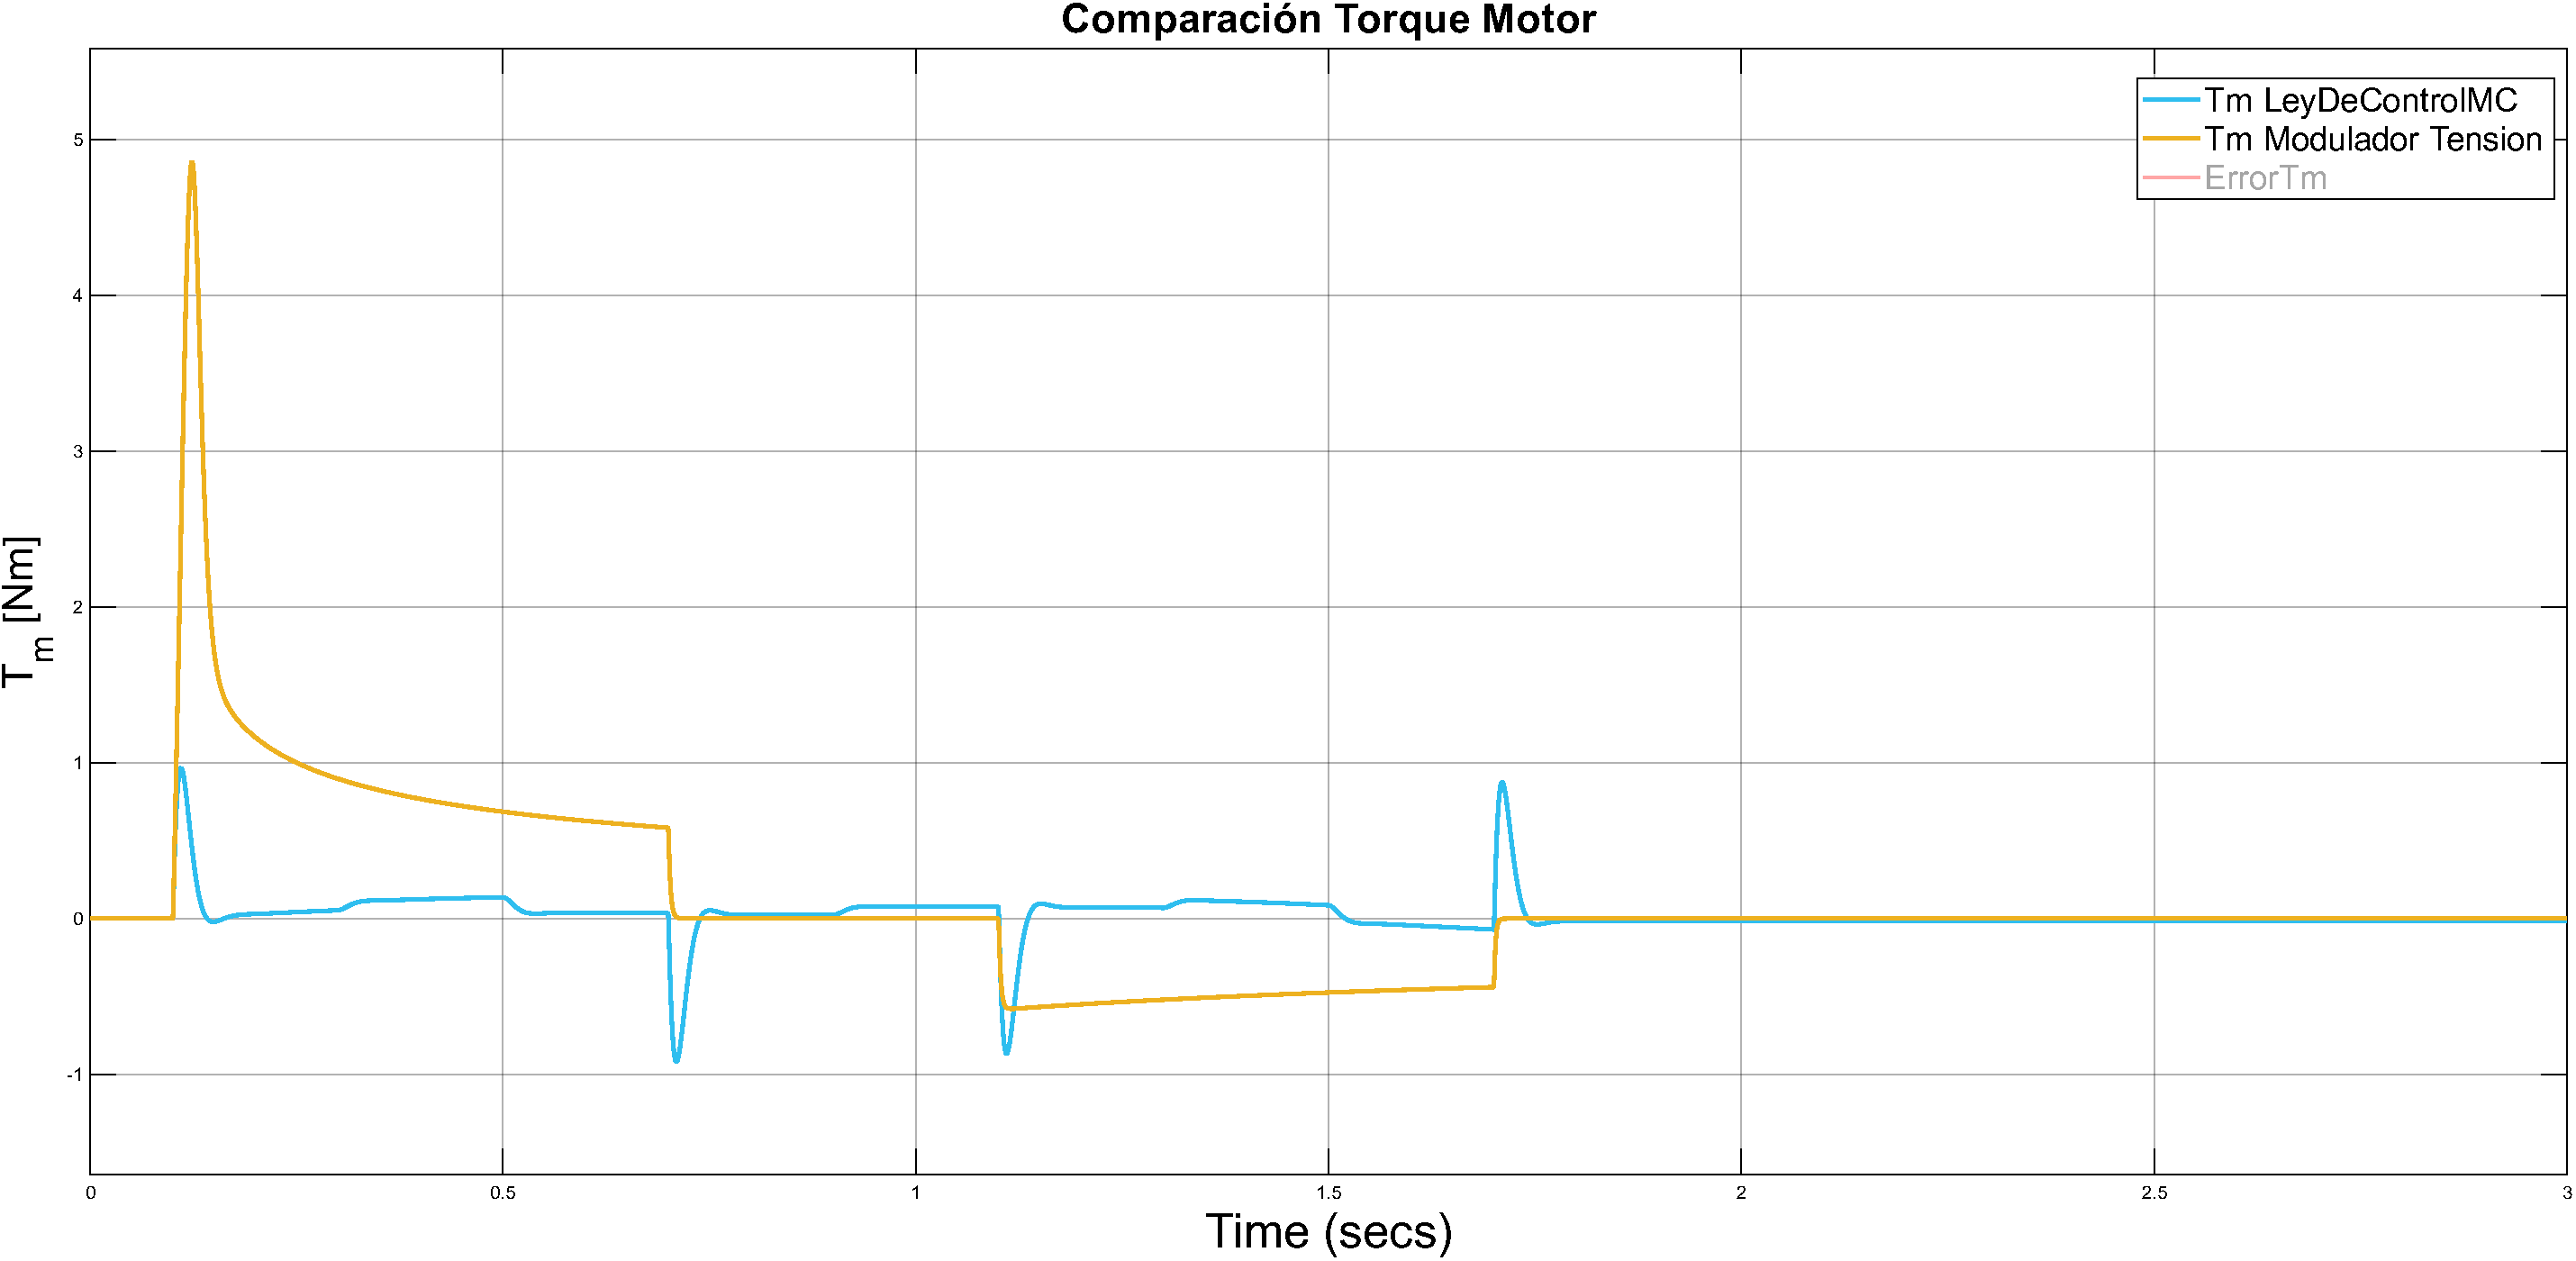
\includegraphics[width=0.95\linewidth]
        {attachments/Tm_LeyCMC_vs_ModTension.pdf}
    \caption{Torque electromagnético del modelo GNL con Ley de
    Control Mínima Complementaria y con Modulador de Tensión
    utilizando resistencia constante en la compensación.}
    \label{fig:tm-leycmc-vs-modtension}
\end{figure}

\begin{figure}[!htbp]
    \centering
    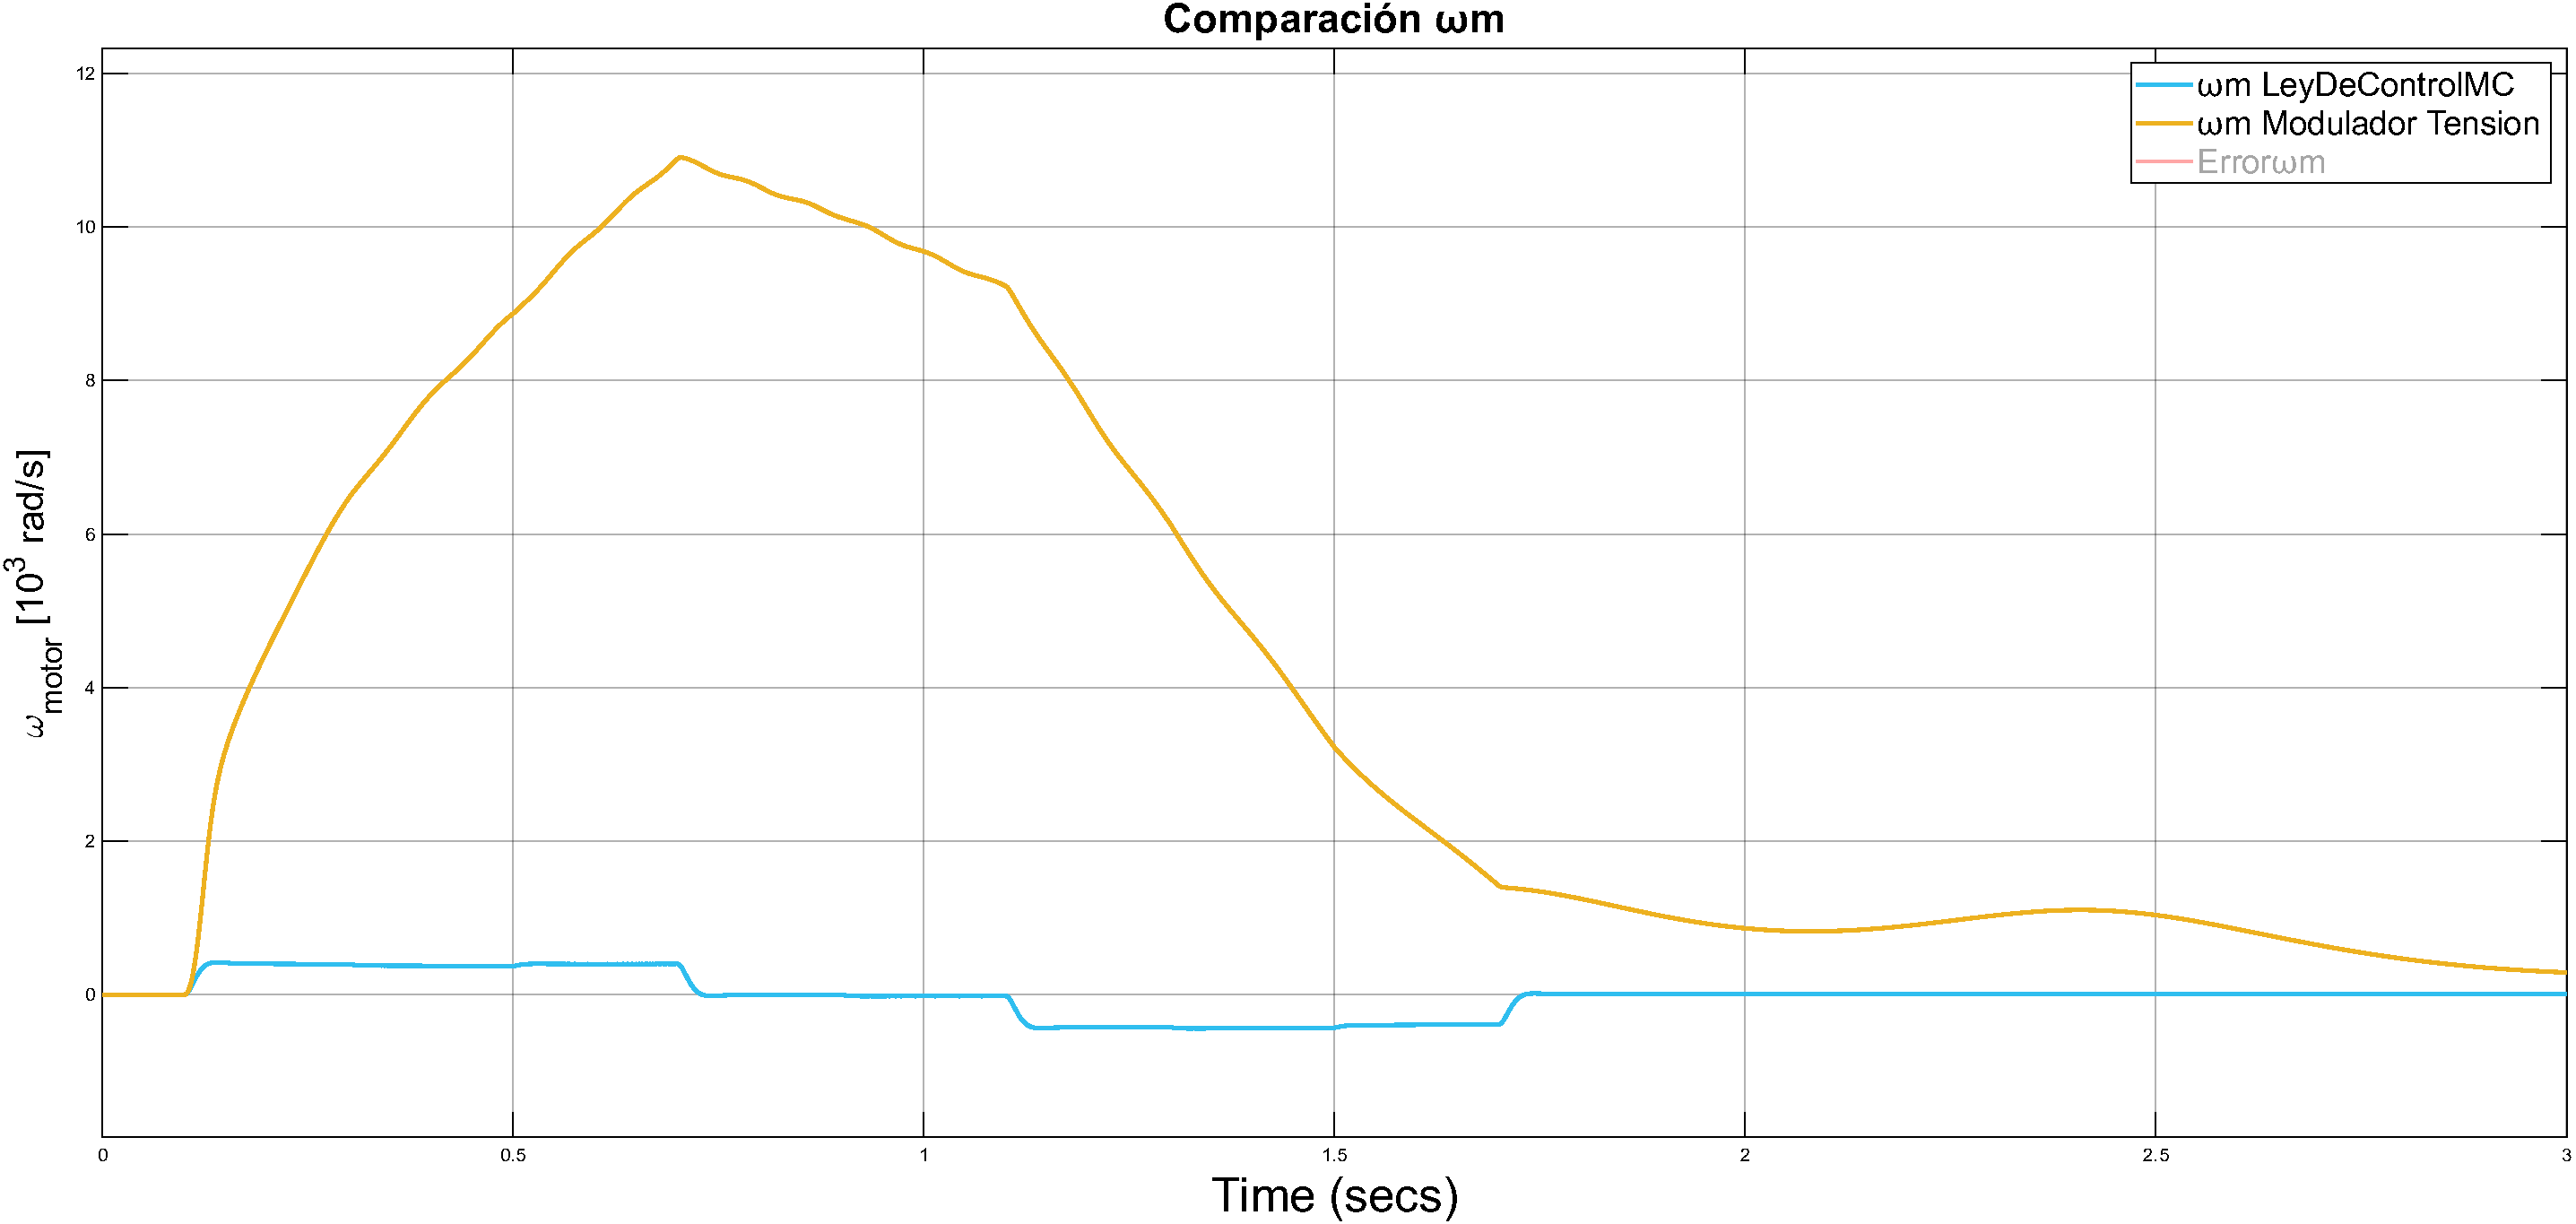
\includegraphics[width=0.95\linewidth]
        {attachments/wm_LeyCMC_vs_ModTension.pdf}
    \caption{Velocidad angular del motor para el modelo GNL con
    Ley de Control Mínima Complementaria y con Modulador de Tensión
    utilizando resistencia constante en la compensación.}
    \label{fig:wm-leycmc-vs-modtension}
\end{figure}

En este ensayo, el Modulador de Tensión produce un pico de torque
y una velocidad considerablemente mayores que los obtenidos
con la Ley de Control Mínima Complementaria. La disminución
del torque después del pico es consistente con la compensación
resistiva incompleta: a medida que aumenta la temperatura,
la resistencia de la planta se aparta del valor constante
utilizado por el modulador, dejando una caída resistiva residual
que limita el crecimiento de la corriente.

Este comportamiento muestra que el desacople eléctrico,
por sí solo, no regula la magnitud de las corrientes. Con
compensación exacta, cada canal equivale a un integrador,
por lo que una tensión virtual constante produce un crecimiento
continuo de la corriente. Para regularla y evitar este
comportamiento, en la siguiente subsección se incorporan los
controladores de corrientes virtuales, que ajustan las tensiones
virtuales para que las corrientes sigan sus respectivas consignas.os que las ecuaciones que rigen las dinámicas de las corrientes son:



% > Comparar la diferencia entre usar $R_{s}(T^{\circ}_{s}(t))$ y utilizar $R_{s}^{\ell}$.

% Realizar gráficos de comparaciones

% ======================================================================================================================================================================================%

\subsubsection{Diseño de los lazos de control de corrientes virtuales con desacoplamiento mutuo y respecto de la velocidad angular}

Una vez compensadas las realimentaciones naturales, cada corriente virtual se regula mediante un controlador proporcional al error de seguimiento. El procedimiento es análogo para los ejes directo, en cuadratura y cero; por ello, se presenta primero un desarrollo general, sin subíndices.

Como criterio de diseño, se fija el polo de cada lazo de corriente en $p=-5000\;\frac{\text{rad}}{\text{seg}}$. Para la respuesta de primer orden resultante, esta elección corresponde a un ancho de banda de $|p|=2\pi f_c=5000\;\frac{\text{rad}}{\text{seg}} \implies f_c \approx 796\; \textbf{Hz}$. La consigna de tensión se define mediante la ley proporcional:
\begin{equation}
\label{eq:regulador-p-corriente}
v^{*}(t) = K_{p} \Big( i^{*}(t) -i(t) \Big)
\end{equation}
Al sustituir la ley \eqref{eq:regulador-p-corriente} en la dinámica de corriente obtenida tras la compensación, resulta:
\[
\frac{di(t)}{dt} = \frac{1}{L} v^{*}(t) =  \frac{1}{L} K_{p} \Big( i^{*}(t) -i(t) \Big)
\]
Aplicando la transformada de Laplace con condiciones iniciales nulas y agrupando los términos en el dominio complejo $s$, se obtiene la función de transferencia de seguimiento de corriente del lazo cerrado:
\begin{align}
\frac{di(t)}{dt}  & = \frac{K_{p}}{L}  \Big( i^{*}(t) -i(t) \Big)
\notag \\
sI & = \frac{K_{p}}{L} \Big( I^{*} - I \Big)
\notag \\
\Big( s + \frac{K_{p}}{L} \Big) I & = \frac{K_{p}}{L} I^{*}
\notag \\
\frac{I}{I^{*}} & = \frac{\frac{K_{p}}{L}}{s+\frac{K_{p}}{L}}=\frac{1}{\frac{L}{K_{p}}s+1}
\label{eq:transferencia-corriente-general}
\end{align}

La transferencia \eqref{eq:transferencia-corriente-general} presenta un polo en $p=-\frac{K_{p}}{L}$. La ganancia $K_p$ tiene dimensión de resistencia, $[\Omega]$, y se denota mediante la letra R para cada eje. Así, las funciones de transferencia particulares son:
\begin{align}
\frac{I_{d}}{I_{d}^{*}} & = \frac{1}{\frac{L_d}{R_{d}}s+1}
\label{eq:transferencia-corriente-d} \\
\frac{I_{q}}{I_{q}^{*}} & = \frac{1}{\frac{L_q}{R_{q}}s+1}
\label{eq:transferencia-corriente-q} \\
\frac{I_{0}}{I_{0}^{*}} & = \frac{1}{\frac{L_{ls}}{R_{0}}s+1}
\label{eq:transferencia-corriente-cero}
\end{align}

Las ganancias necesarias para ubicar los tres polos en el valor especificado se calculan como:
\begin{equation}
\label{eq:ganancias-corriente}
p = -\frac{R}{L} \implies \begin{cases}
R_{d} & = 5000 L_{d} = 33\; [\Omega] \\
R_{q} & = 5000 L_{q} = 29\; [\Omega]\\
R_{0} & = 5000 L_{ls} = 4\; [\Omega]
\end{cases}
\end{equation}

\clearpage
\begin{figure}[!htbp]
    \centering
    \begin{adjustbox}{max totalsize={\linewidth}{0.65\textheight},center}
        \begin{minipage}{\linewidth}
            \centering
            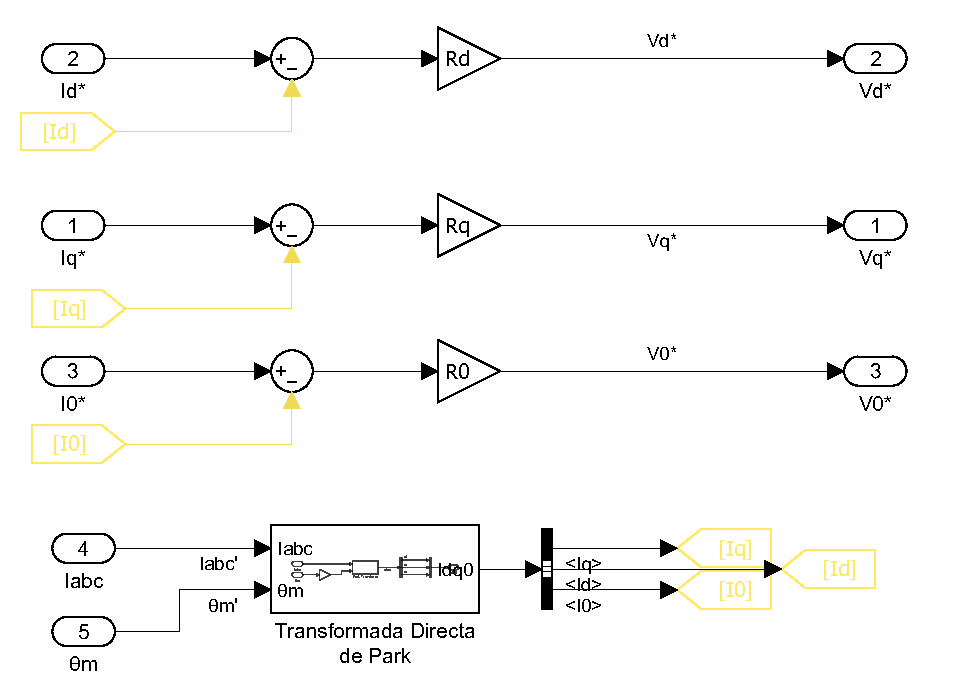
\includegraphics[width=\linewidth]{attachments/Lazo de Control de Corrientes Virtuales.pdf}
            \par\vspace{4mm}
            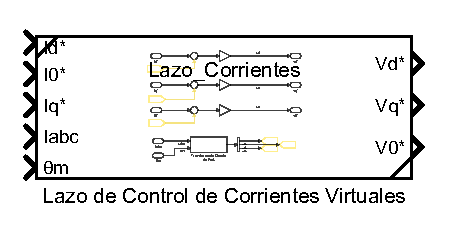
\includegraphics[width=0.42\linewidth,height=0.19\textheight,keepaspectratio]{attachments/Bloque Lazo de Control de Corrientes Virtuales.pdf}
        \end{minipage}
    \end{adjustbox}
    \caption{Bloque de controlador proporcional de las corrientes virtuales}
    \label{fig:ControladorCorrientesVirtuales}
\end{figure}

% > ¿Qué provoca agregar acción integral? Investigar sus consecuencias.

% ======================================================================================================================================================================================%
\subsubsection{Compensación del torque de carga por gravedad}

El paso siguiente consiste en definir las referencias de corriente a partir de la consigna de torque. Como condición inicial de diseño, se adoptan las siguientes consignas:
\begin{equation}
\label{eq:referencias-corriente}
\begin{aligned}
i_{ds}^{*r}(t) & = 0 \\
i_{qs}^{*r}(t) & \neq 0 \\
i_{0s}^{*r}(t) & = 0
\end{aligned}
\end{equation}

La corriente en cuadratura permite regular el torque útil, mientras que la corriente directa modifica el campo magnético y la corriente homopolar solo introduce pérdidas. Aunque puede considerarse el caso $i_{ds}^{*r}(t) \neq 0$ para debilitar o reforzar el campo (\textit{field weakening} o \textit{field forcing}, según el signo de la corriente), el estudio comienza con $i_{ds}^{*r}(t) = 0$.

Para compensar la fricción viscosa equivalente y el torque gravitatorio de la carga, se retoma la ecuación de la velocidad angular del motor:

\begin{equation}
\label{eq:dinamica-mecanica-torque}
\frac{d\omega_{m}(t)}{dt} = \frac{1}{J_{eq}} \Bigg[ \frac{3}{2}P_{p} \lambda_{m}^{'r} i_{qs}^{r}(t) + \frac{3}{2} P_{p} \Big( L_{d} - L_{q} \Big) i_{qs}^{r}(t) i_{ds}^{r}(t) - b_{eq}  \omega_{m}(t)   - \frac{1}{r} T_{dl}(t) - \frac{k_{l}g}{r} \sin \left(  \frac{1}{r} \theta_{m}(t) \right) \Bigg]
\end{equation}

El objetivo es obtener la siguiente relación entre la consigna de torque y la aceleración angular:
\begin{equation}
\label{eq:objetivo-mecanico-ideal}
\frac{d\omega_{m}(t)}{dt} = \frac{T_{m}^{*}(t)}{J_{eq}} 
\end{equation}

El torque $T_{dl}$ constituye una \textbf{perturbación de la carga mecánica}, cuya magnitud y evolución temporal se consideran desconocidas para el controlador. Por esta razón, no se incorpora a la ley de compensación. El torque solicitado al motor incluye la consigna de movimiento y las compensaciones viscosa y gravitatoria:

\begin{align}
T_{m}(t) & = T_{m}^{*}(t) +b_{eq}\omega_{m}(t) + \frac{k_{l}g}{r} \sin \left( \frac{1}{r} \theta_{m}(t)  \right)
\label{eq:torque-compensado} \\
T_{m}(t) & \approx \frac{3}{2}P_{p} \Big[ \lambda_{m}^{'r} + \Big( L_{d}-L_{q} \Big)i_{ds}^{r}(t) \Big] i_{qs}^{*r}(t)
\notag
\end{align}

Al despejar la referencia de corriente en cuadratura, se obtiene:

\begin{equation}
\label{eq:referencia-iq}
i_{qs}^{*r}(t) = \frac{T_{m}^{*}(t) +b_{eq}\omega_{m}(t) + \frac{k_{l}g}{r} \sin \left( \frac{1}{r} \theta_{m}(t)  \right)}{\frac{3}{2}P_{p} \Big[ \lambda_{m}^{'r} + \Big( L_{d}-L_{q} \Big)i_{ds}^{r}(t) \Big]}
\end{equation}

\begin{figure}[!htbp]
    \centering
    \begin{adjustbox}{max totalsize={0.75\linewidth}{0.65\textheight},center}
        \begin{minipage}{\linewidth}
            \centering
            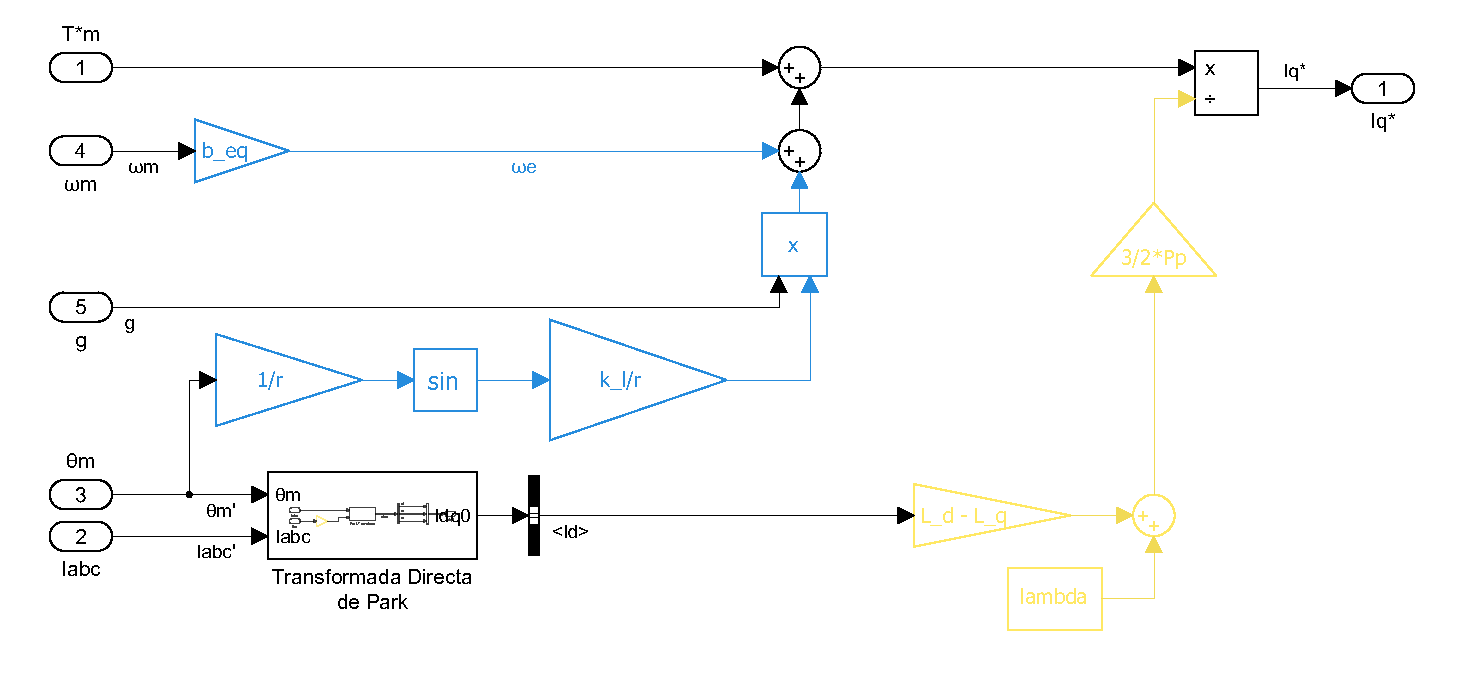
\includegraphics[width=\linewidth]{attachments/Modulador y Compensación de Torque.pdf}
            \par\vspace{4mm}
            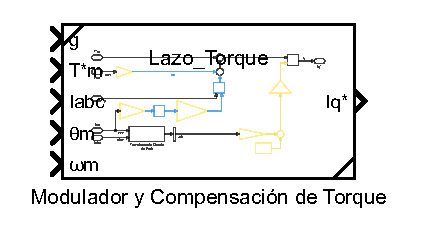
\includegraphics[width=0.42\linewidth,height=0.19\textheight,keepaspectratio]{attachments/Bloque Modulador y Compensación de Torque.pdf}
        \end{minipage}
    \end{adjustbox}
    \caption{Bloque de compensación de torque gravitatorio y modulación torque}
    \label{fig:CompensacionTorqueG}
\end{figure}

\subsubsection{Diseño final del modulador de Torque Equivalente}

Finalmente, el bloque del modulador de torque equivalente, con retroalimentación no lineal en el calculo de tensiones virtuales, control de corrientes virtuales con asignación de polos, compensación de torque gravitatorio y compensación de fricción queda tal que:

\begin{figure}[!htbp]
    \centering
    \begin{adjustbox}{max totalsize={\linewidth}{0.65\textheight},center}
        \begin{minipage}{\linewidth}
            \centering
            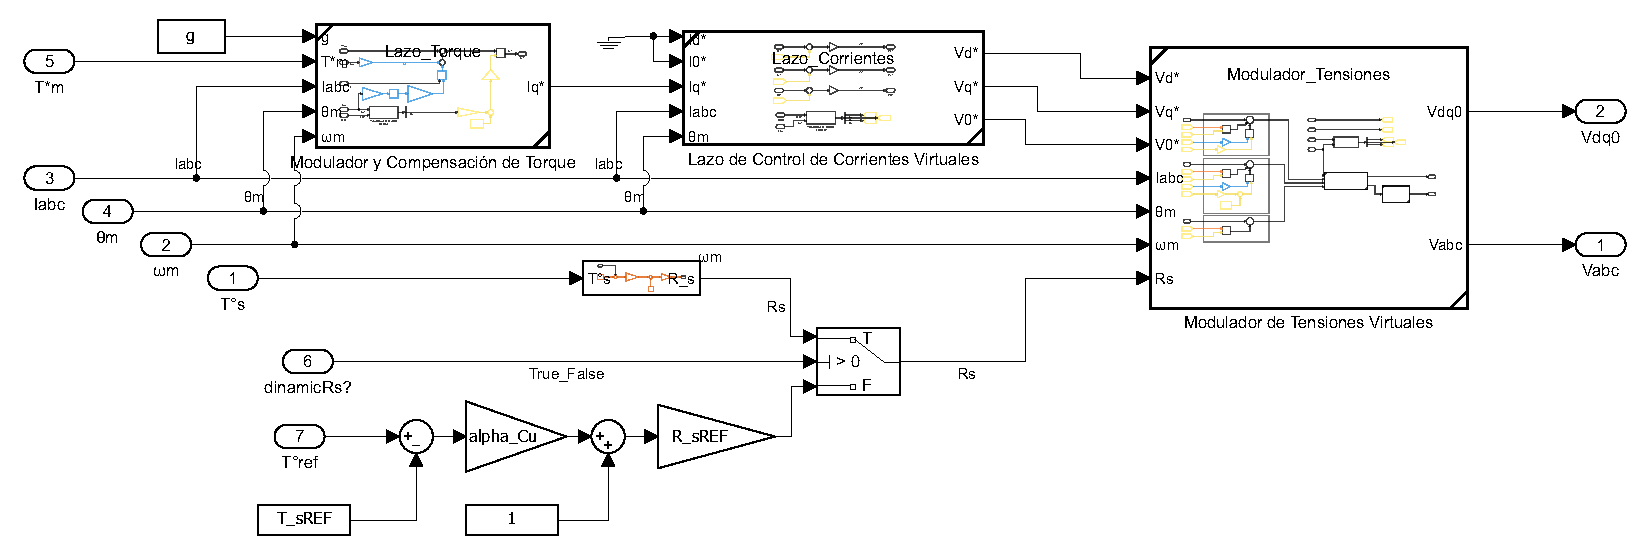
\includegraphics[width=\linewidth]{attachments/Modulador de Torque Equivalente.pdf}
            \par\vspace{4mm}
            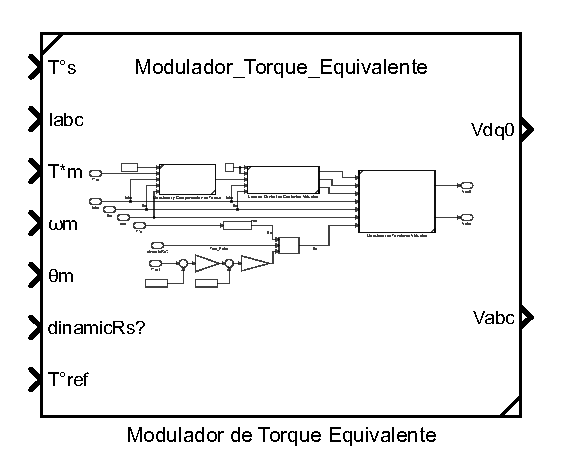
\includegraphics[width=0.42\linewidth,height=0.19\textheight,keepaspectratio]{attachments/Bloque Modulador de Torque Equivalente.pdf}
        \end{minipage}
    \end{adjustbox}
    \caption{Bloque de modulador de torque equivalente, integrando los bloques de la modulación de tensión virtual, el control de corrientes virtuales y la compensación de torque gravitatorio y fricción.}
    \label{fig:ModTorqueEquiv}
\end{figure}

Se compara el comportamiento del modelo Global No Lineal (GNL)
con Modulador de Torque Equivalente y con Ley de Control Mínima
Complementaria. Ambas estrategias utilizan variables de entrada
diferentes: la primera recibe una consigna de torque referida al
eje motor, $T_m^*(t)$, mientras que la segunda recibe una consigna
de tensión virtual en el eje de cuadratura, $v_{qs}^{*r}(t)$.

Para establecer un criterio común de ensayo, se conserva el
perfil temporal de la consigna de tensión definida previamente,
incluidos sus instantes de aplicación, retiro e inversión de
signo. Este perfil se utiliza también para la consigna de torque,
ajustando su amplitud a $0.375\;\mathrm{N\,m}$. La comparación
permite observar las diferencias de respuesta entre ambas
estrategias ante una misma secuencia temporal de excitación,
sin suponer que las entradas de tensión y torque sean
físicamente equivalentes ni que deban producir la misma
trayectoria de movimiento.

La amplitud de torque se selecciona tomando como referencia el
torque pico de salida del reductor,
$T_{q,\mathrm{max}}=45\;\mathrm{N\,m}$. Para una relación de
reducción $r=120$, su valor referido al eje motor es:
\begin{equation}
    \left|T_m^*\right|_{\mathrm{max}}
    = \frac{T_{q,\mathrm{max}}}{r}
    = \frac{45}{120}
    = 0.375\;\mathrm{N\,m}.
\end{equation}

Esta elección establece una escala de referencia para la
consigna de torque de movimiento. Sin embargo, no garantiza
por sí sola el cumplimiento del límite de torque del reductor,
ya que el Modulador de Torque Equivalente incorpora
adicionalmente las compensaciones de fricción viscosa y
gravedad. En consecuencia, el torque electromagnético
solicitado puede superar la consigna $T_m^*$, y el torque
efectivamente transmitido a la carga debe verificarse a partir
de la respuesta del sistema.

La Figura~\ref{fig:entrada-modulador-torque-equiv} presenta los
estímulos utilizados en el ensayo. Para comparar las respuestas,
se mantienen iguales los parámetros físicos, las condiciones
iniciales y la perturbación de carga aplicada a ambas ramas.

\begin{figure}[!htbp]
    \centering
    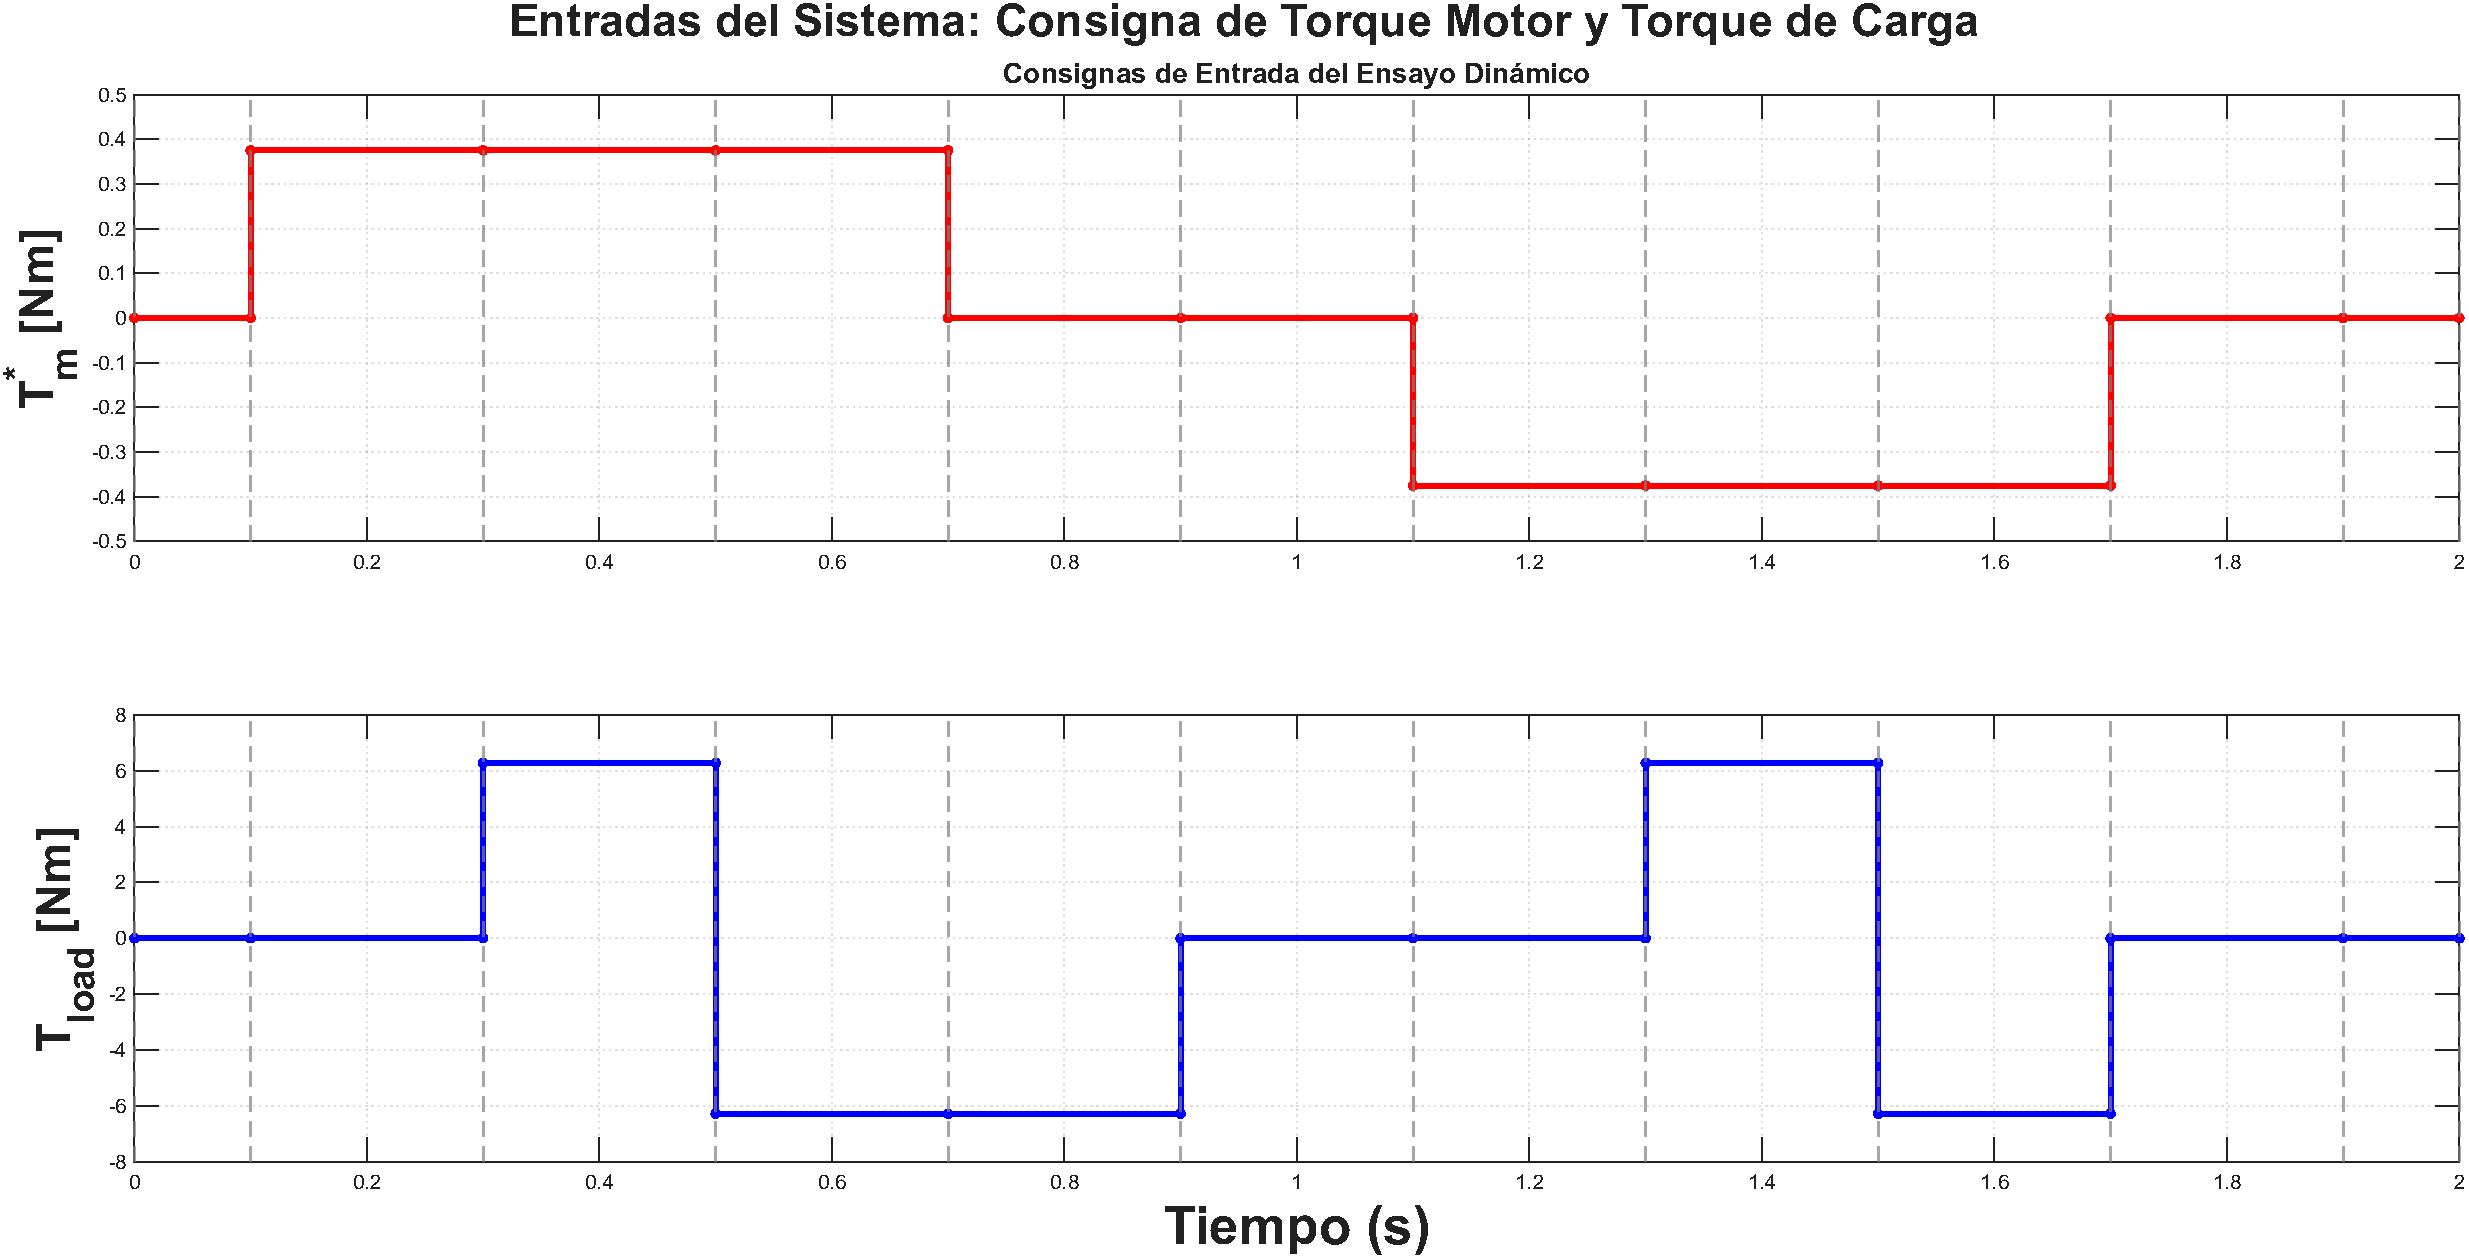
\includegraphics[width=0.95\linewidth]
        {attachments/Estímulos de Entrada para Simulación Modulador Torque Equiv.pdf}
    \caption{Consigna de torque del motor (arriba) y perturbación de torque de carga (abajo) en el ensayo comparativo. La consigna de tensión de la otra rama sigue la secuencia temporal de la Figura~\ref{fig:entradas-modulador-tension}.}
    \label{fig:entrada-modulador-torque-equiv}
\end{figure}

Las Figuras~\ref{fig:thetam-leycmc-vs-modteq}
a~\ref{fig:ts-leycmc-vs-modteq} muestran las respuestas de posición,
velocidad angular, torque electromagnético, corriente en
cuadratura y temperatura del bobinado. Estas variables permiten
evaluar el efecto de la regulación interna de corriente y de
las compensaciones incorporadas por el modulador sobre el
movimiento y el esfuerzo eléctrico y térmico del accionamiento.

\begin{figure}[!htbp]
    \centering
    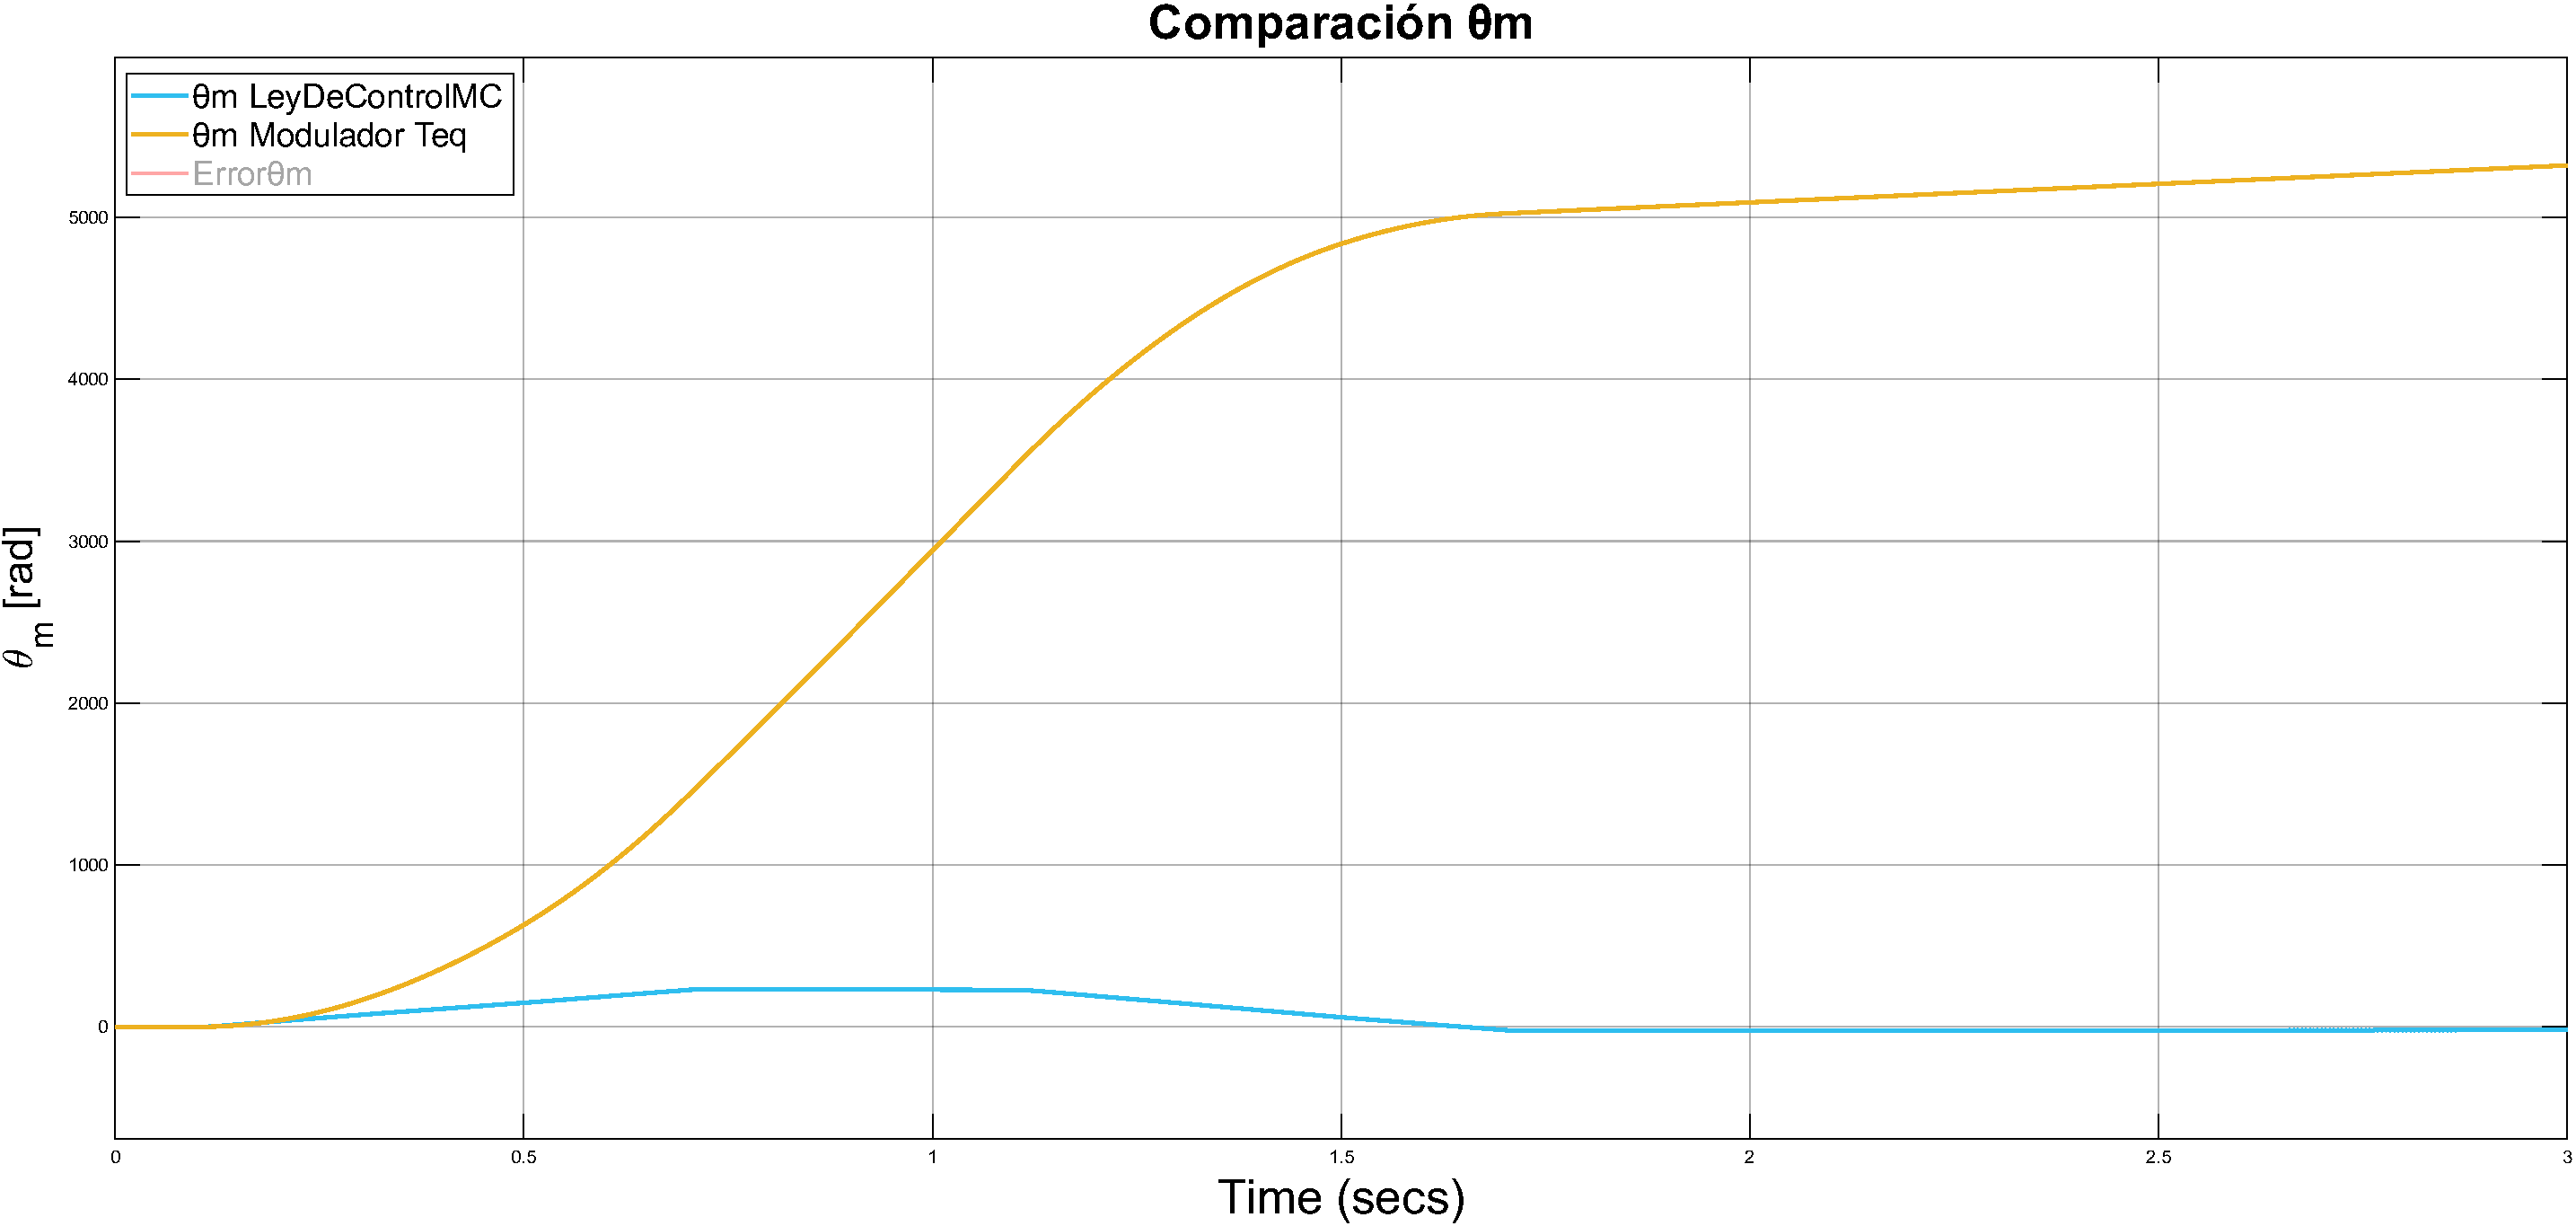
\includegraphics[width=0.95\linewidth]
        {attachments/thetam_LeyCMC_vs_ModTeq.pdf}
    \caption{Comparación de la posición angular del motor
    $\theta_m$ entre el modelo GNL con Ley de Control Mínima
    Complementaria y con Modulador de Torque Equivalente.}
    \label{fig:thetam-leycmc-vs-modteq}
\end{figure}

\begin{figure}[!htbp]
    \centering
    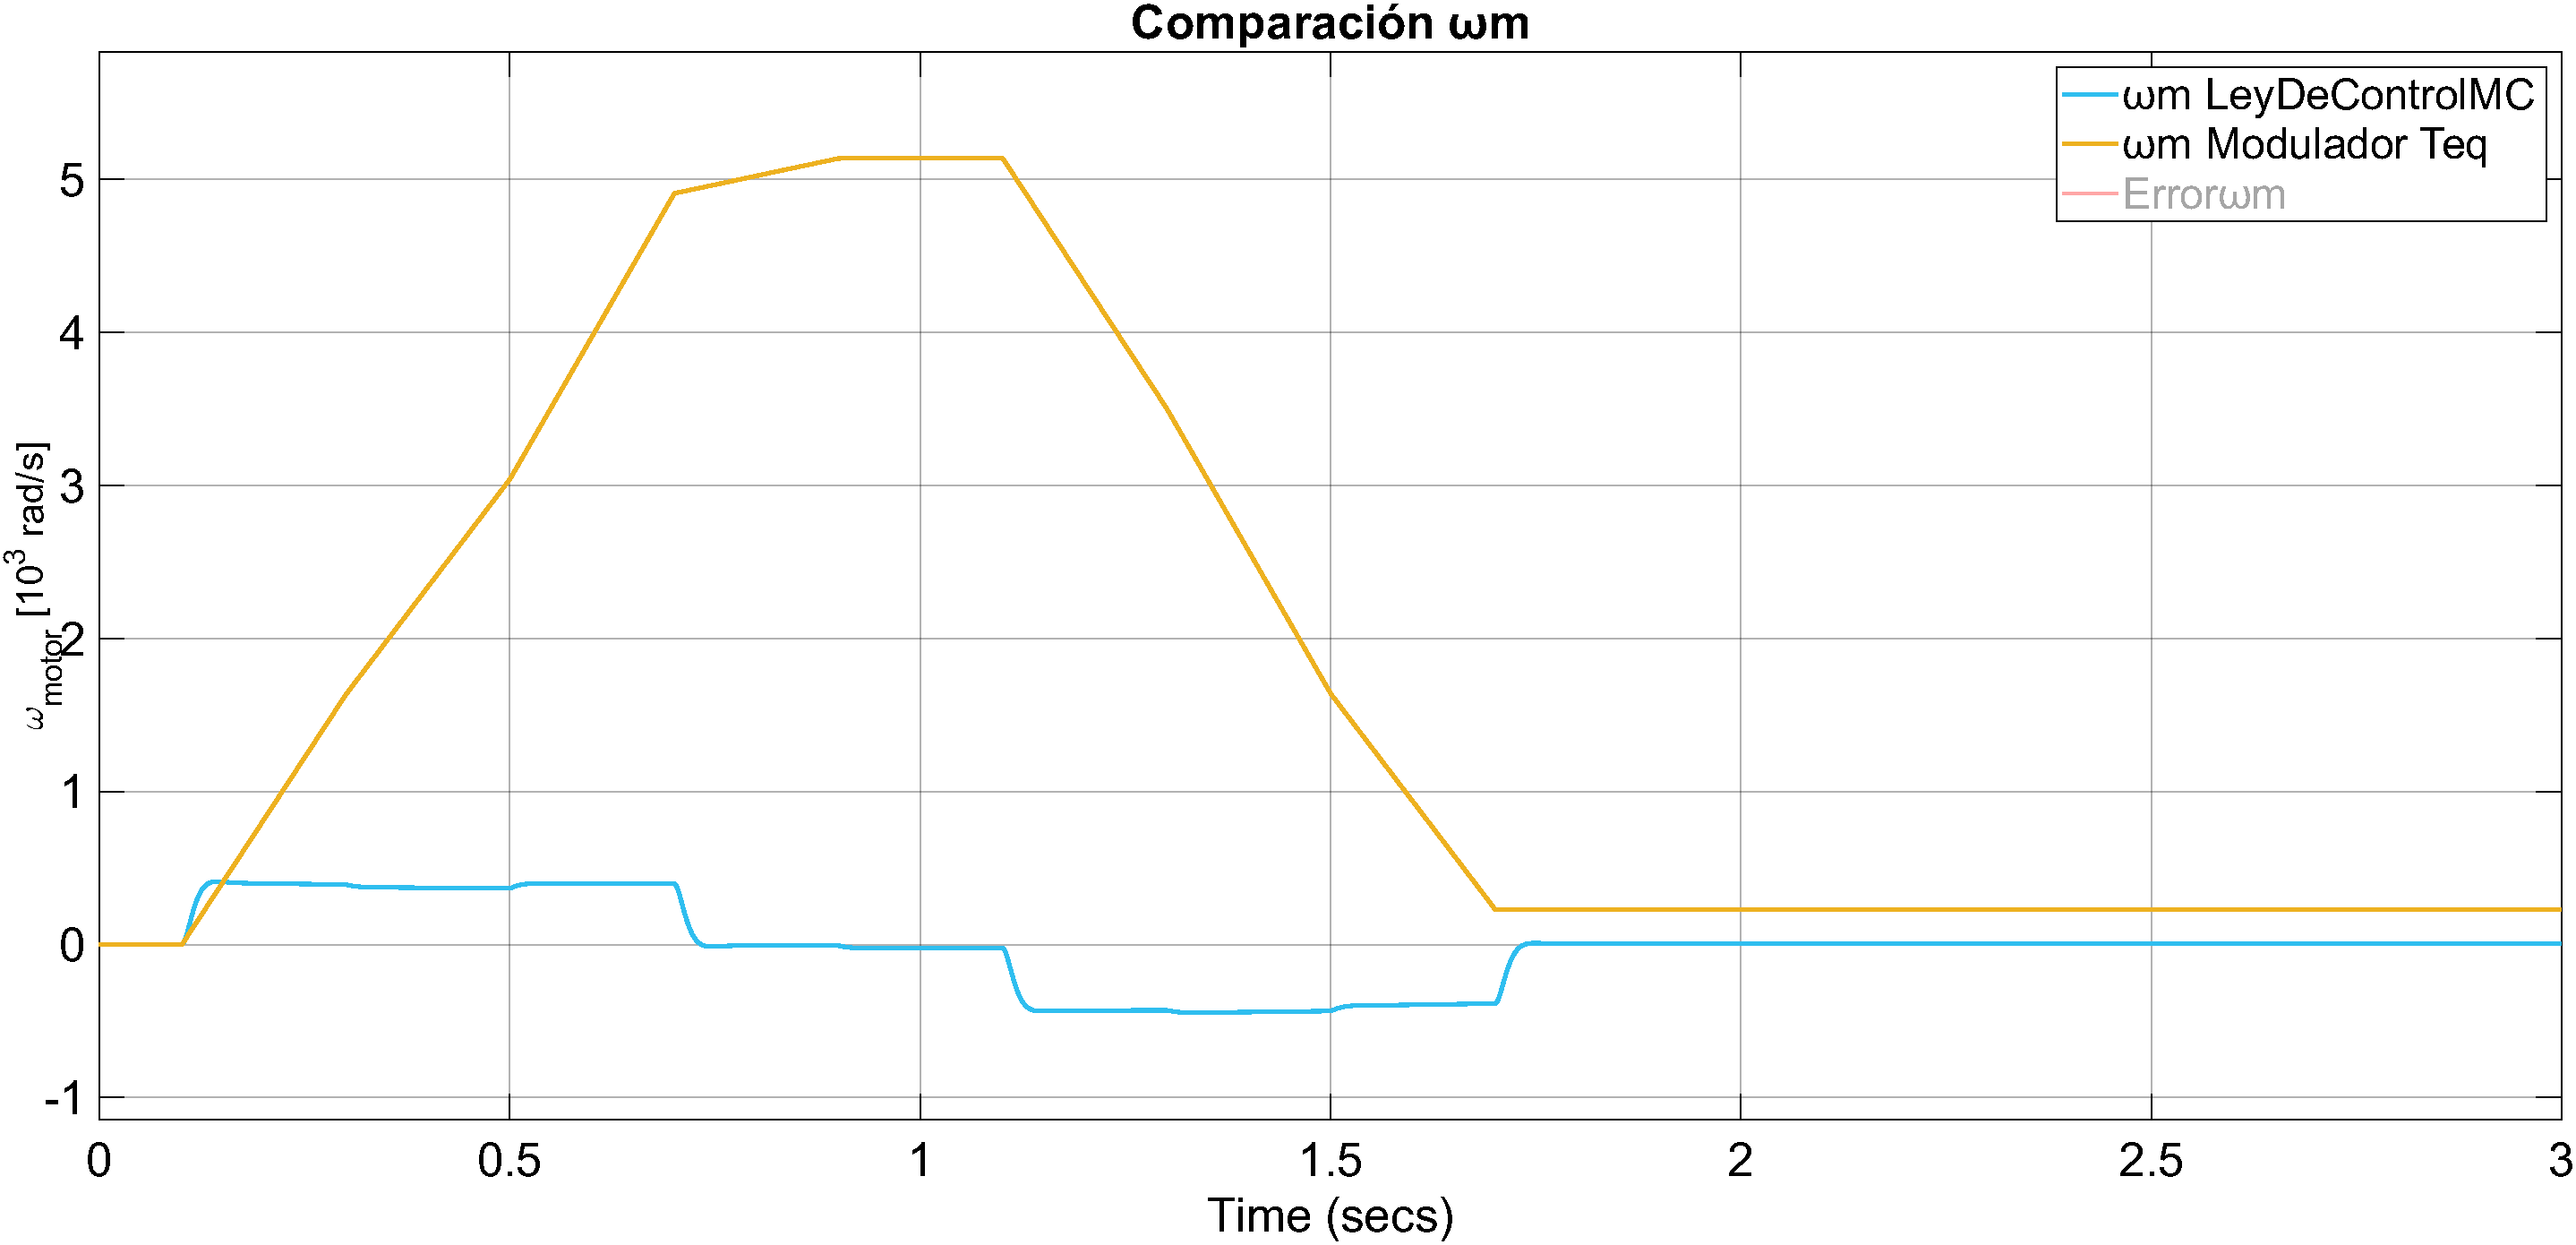
\includegraphics[width=0.95\linewidth]{attachments/wm_LeyCMC_vs_ModTeq.pdf}
    \caption{Comparación de la velocidad angular del motor
    $\omega_m$ entre el modelo GNL con Ley de Control Mínima
    Complementaria y con Modulador de Torque Equivalente.}
    \label{fig:wm-leycmc-vs-modteq}
\end{figure}

\begin{figure}[!htbp]
    \centering
    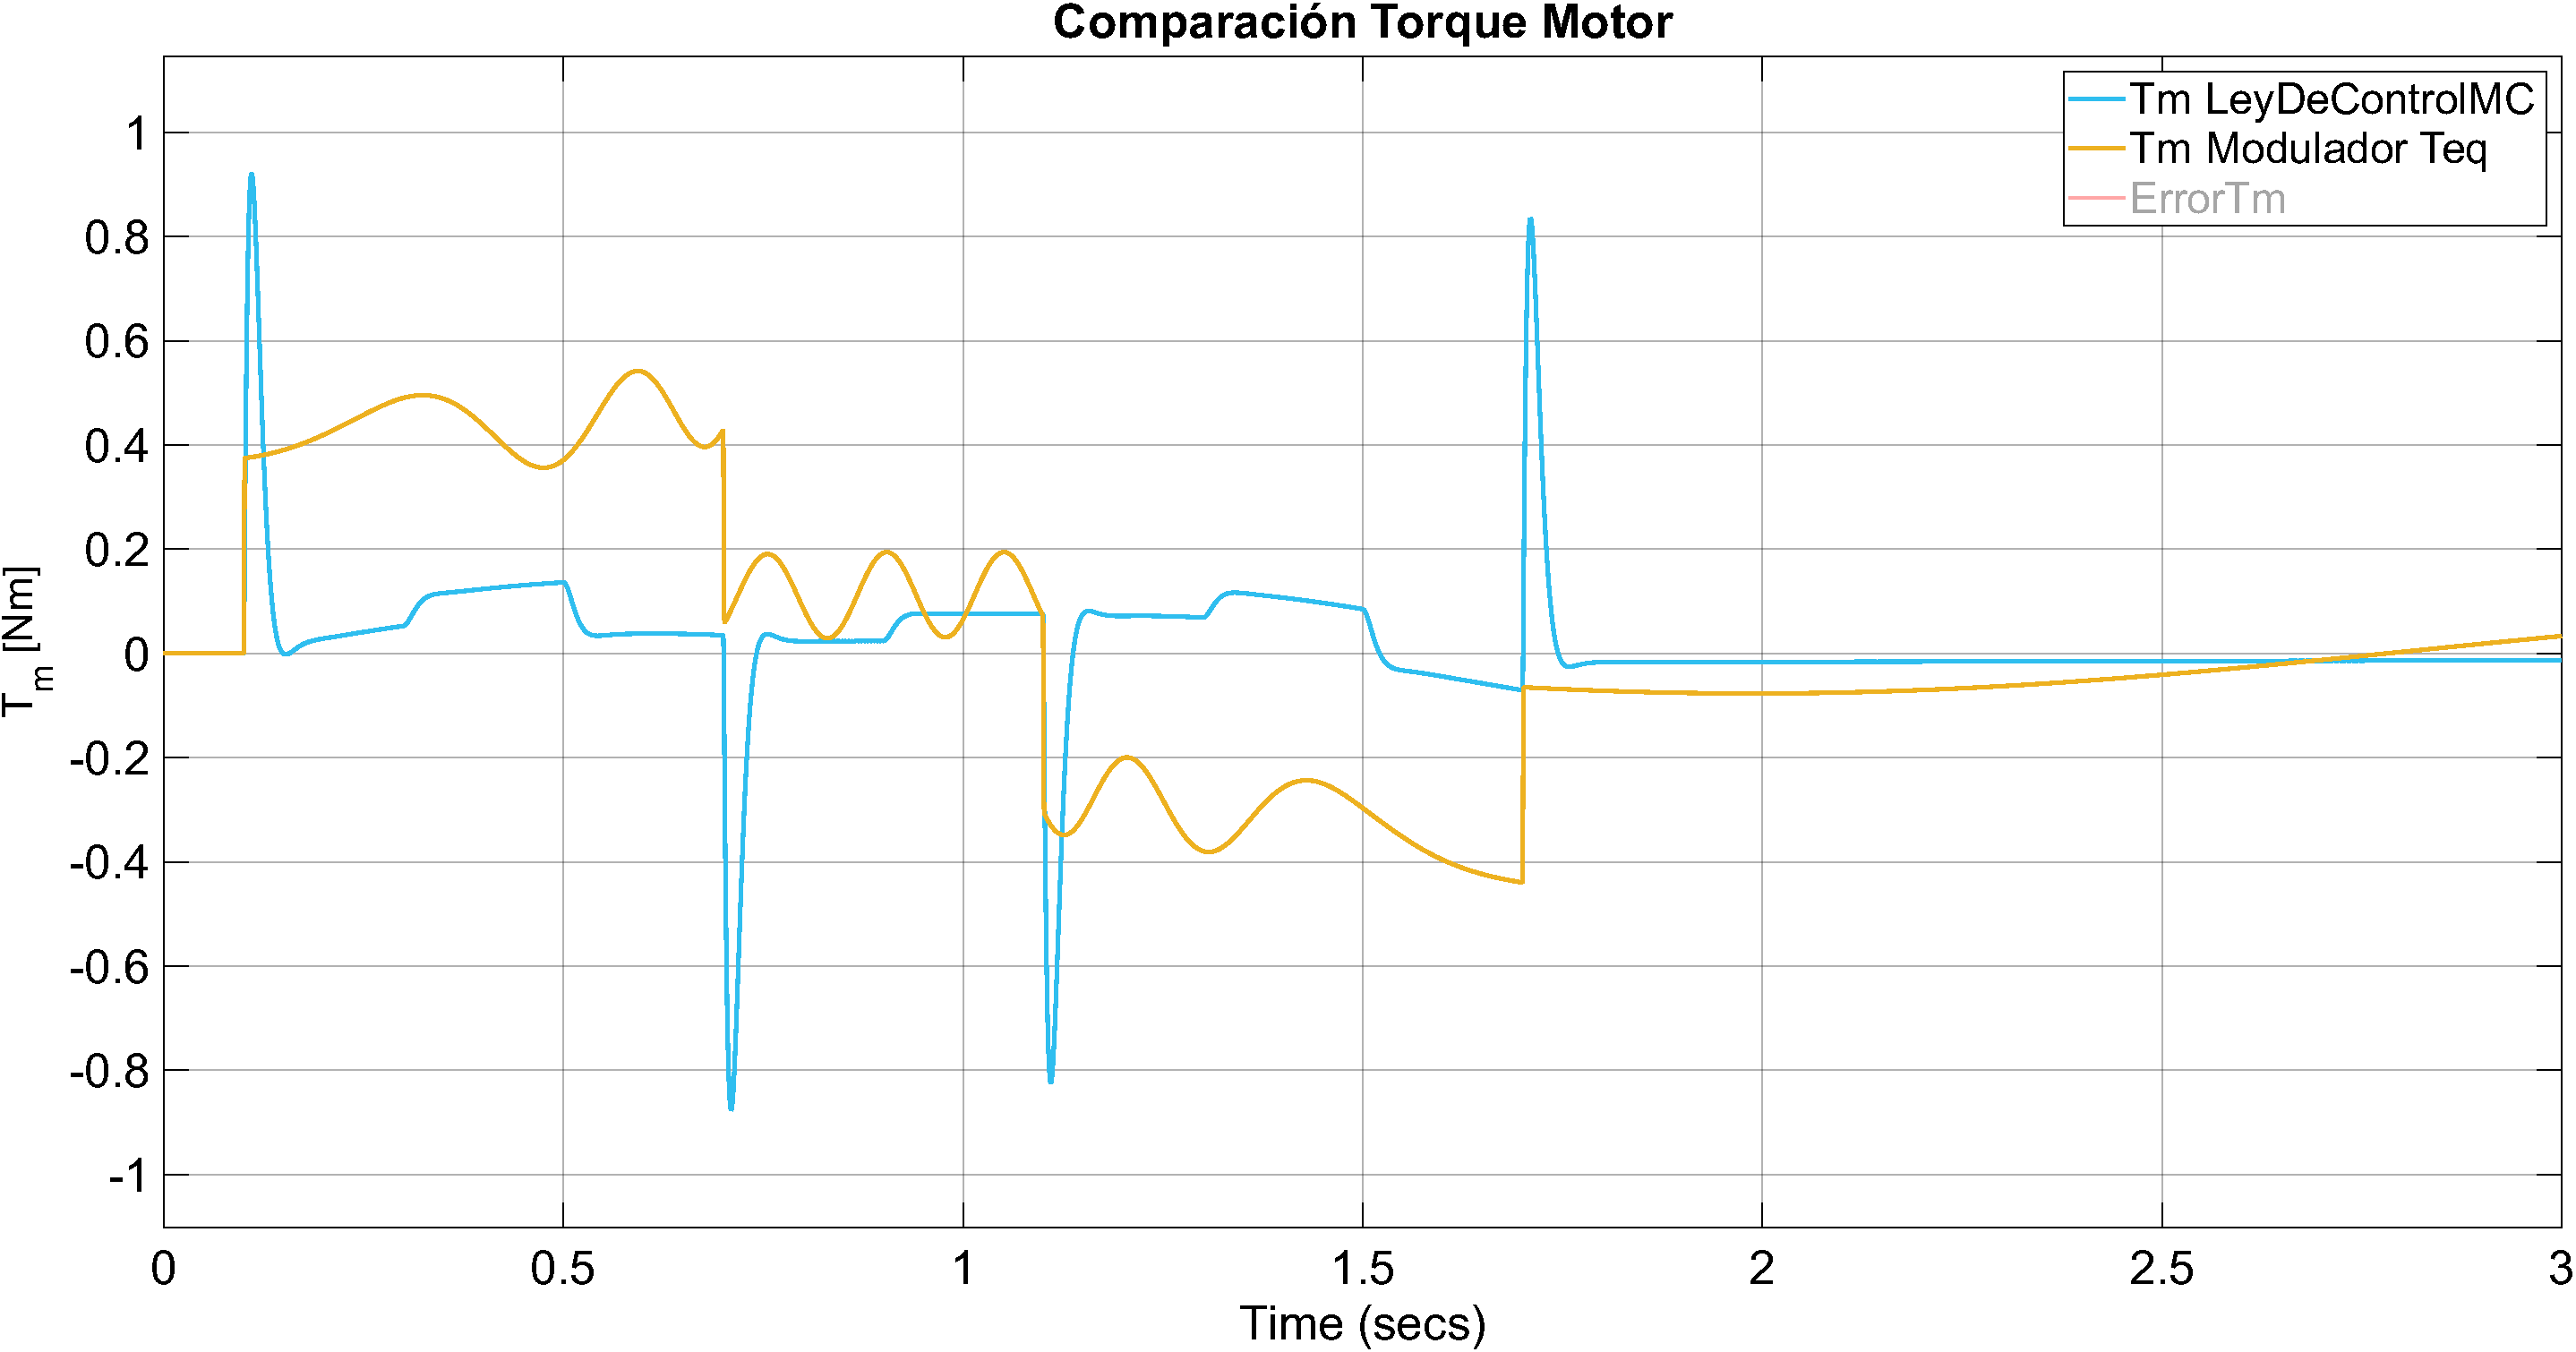
\includegraphics[width=0.95\linewidth]
        {attachments/Tm_LeyCMC_vs_ModTeq.pdf}
    \caption{Comparación del torque electromagnético $T_m$
    entre el modelo GNL con Ley de Control Mínima Complementaria
    y con Modulador de Torque Equivalente.}
    \label{fig:tm-leycmc-vs-modteq}
\end{figure}

\begin{figure}[!htbp]
    \centering
    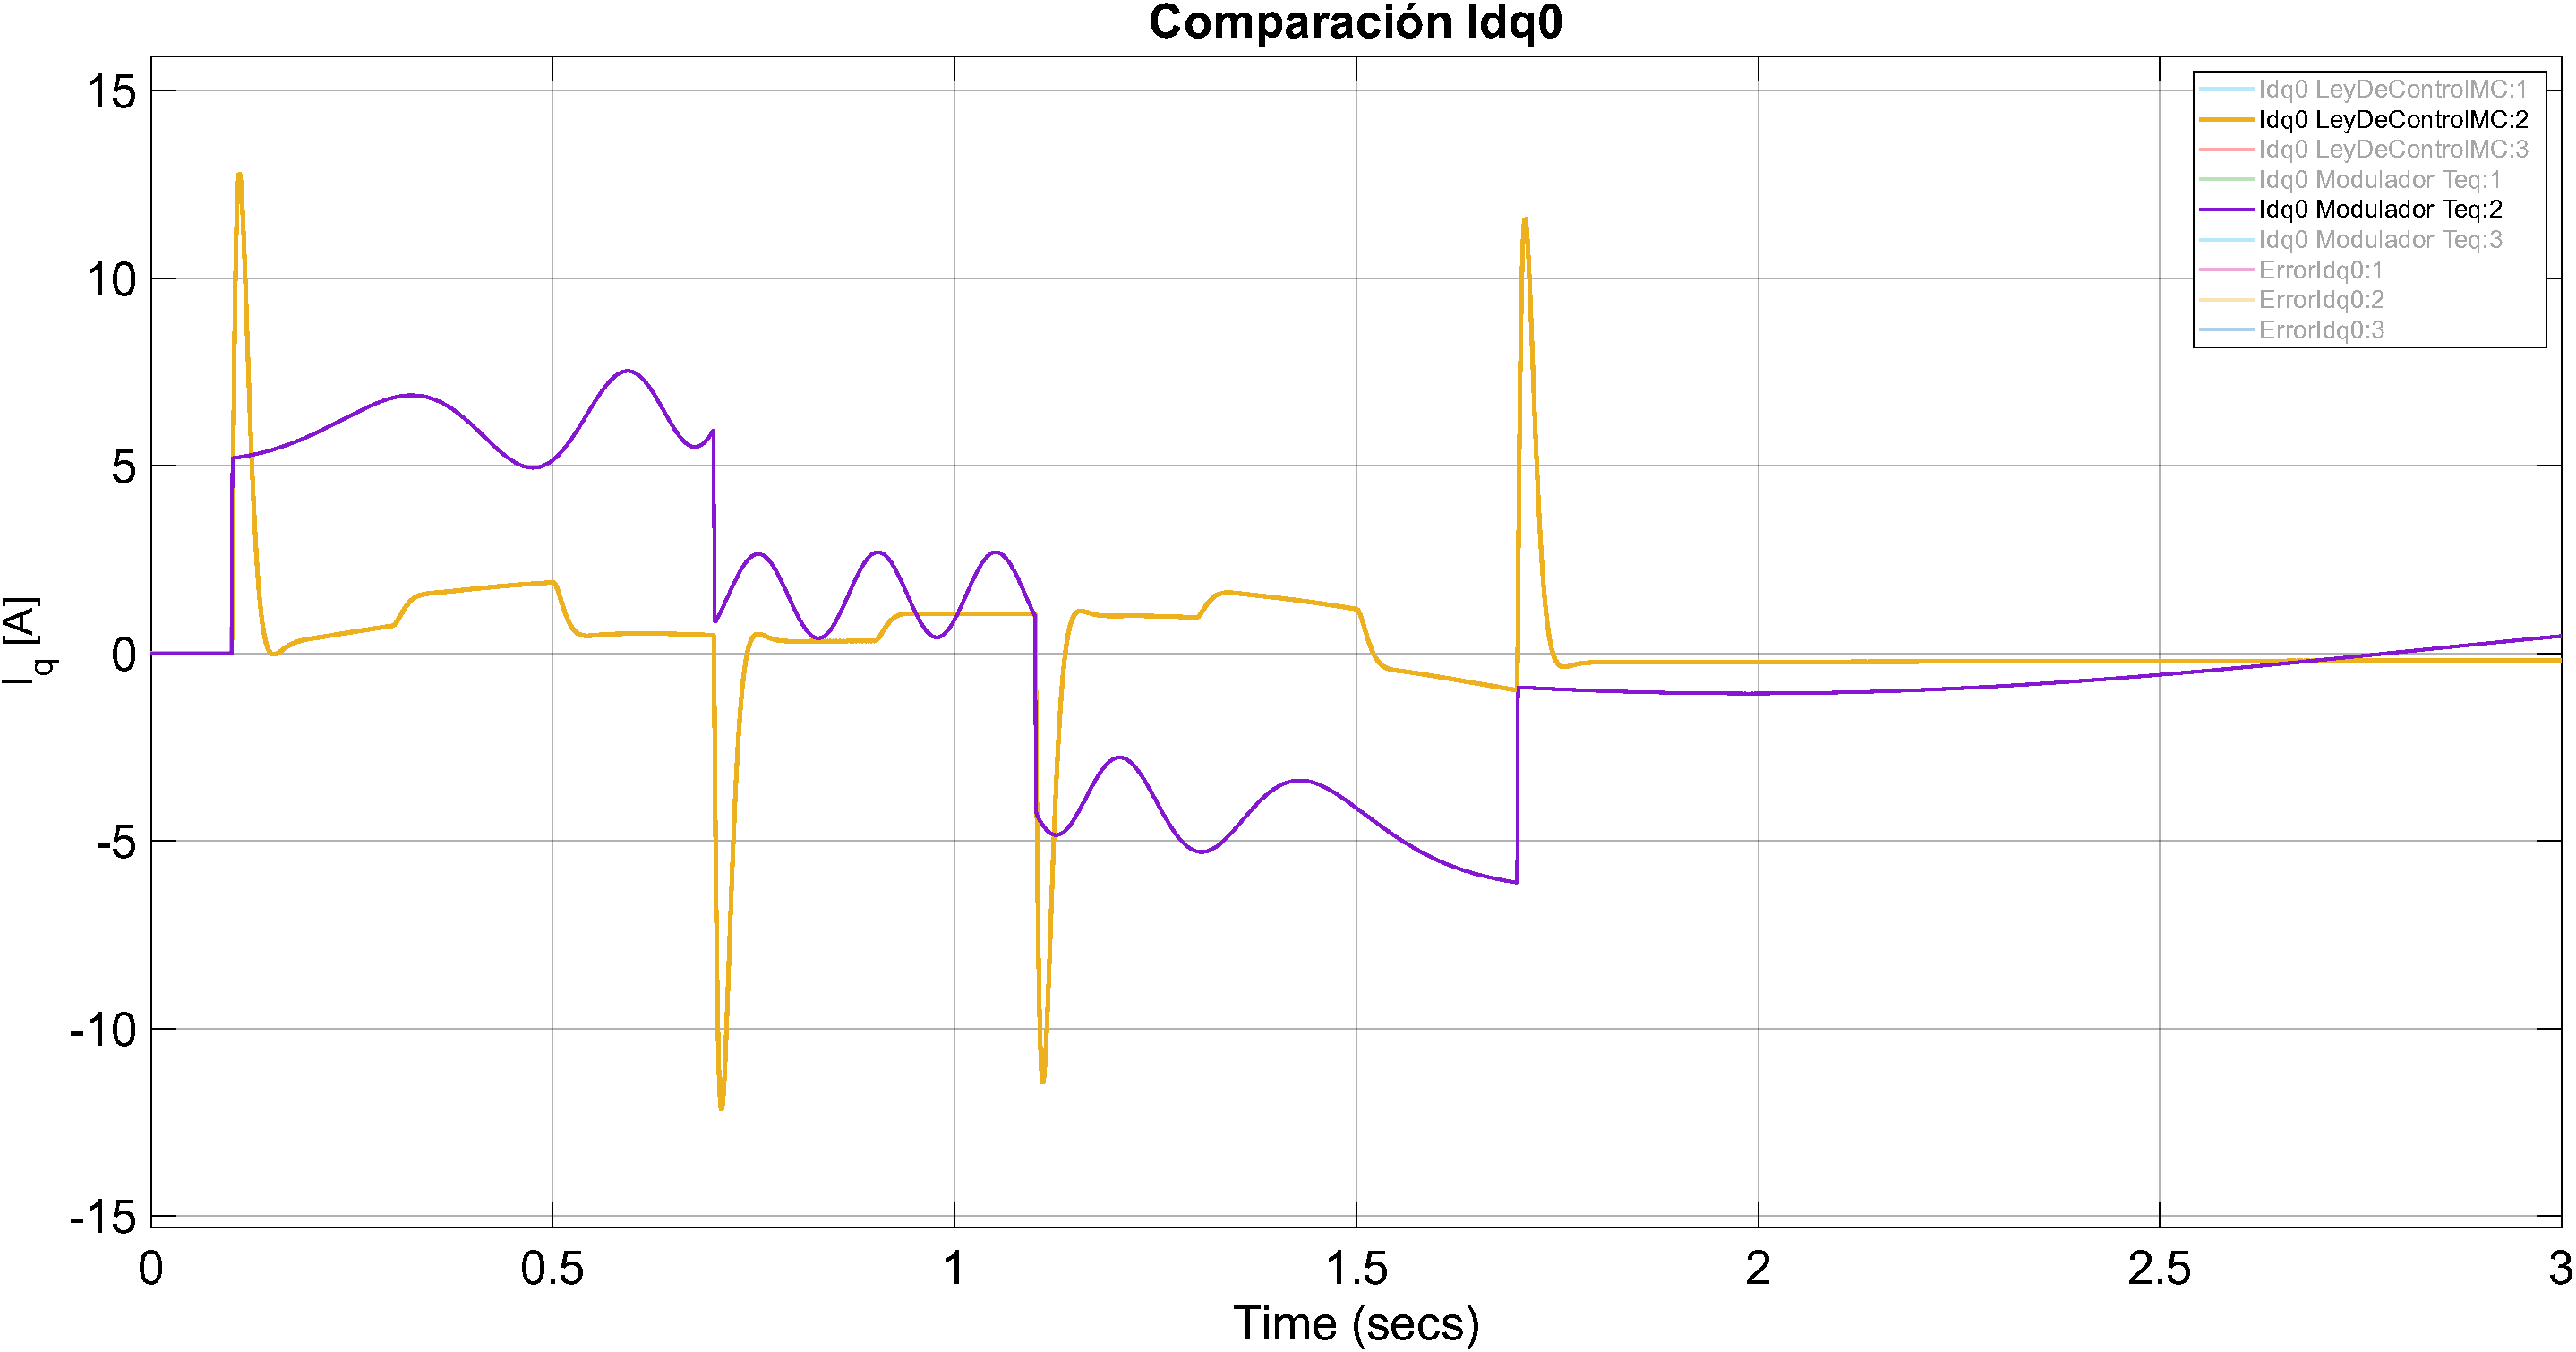
\includegraphics[width=0.95\linewidth]
        {attachments/Iq_LeyCMC_vs_ModTeq.pdf}
    \caption{Comparación de las corrientes virtuales $i_{dq0}$
    entre el modelo GNL con Ley de Control Mínima
    Complementaria y con Modulador de Torque Equivalente.}
    \label{fig:iq-leycmc-vs-modteq}
\end{figure}

\begin{figure}[!htbp]
    \centering
    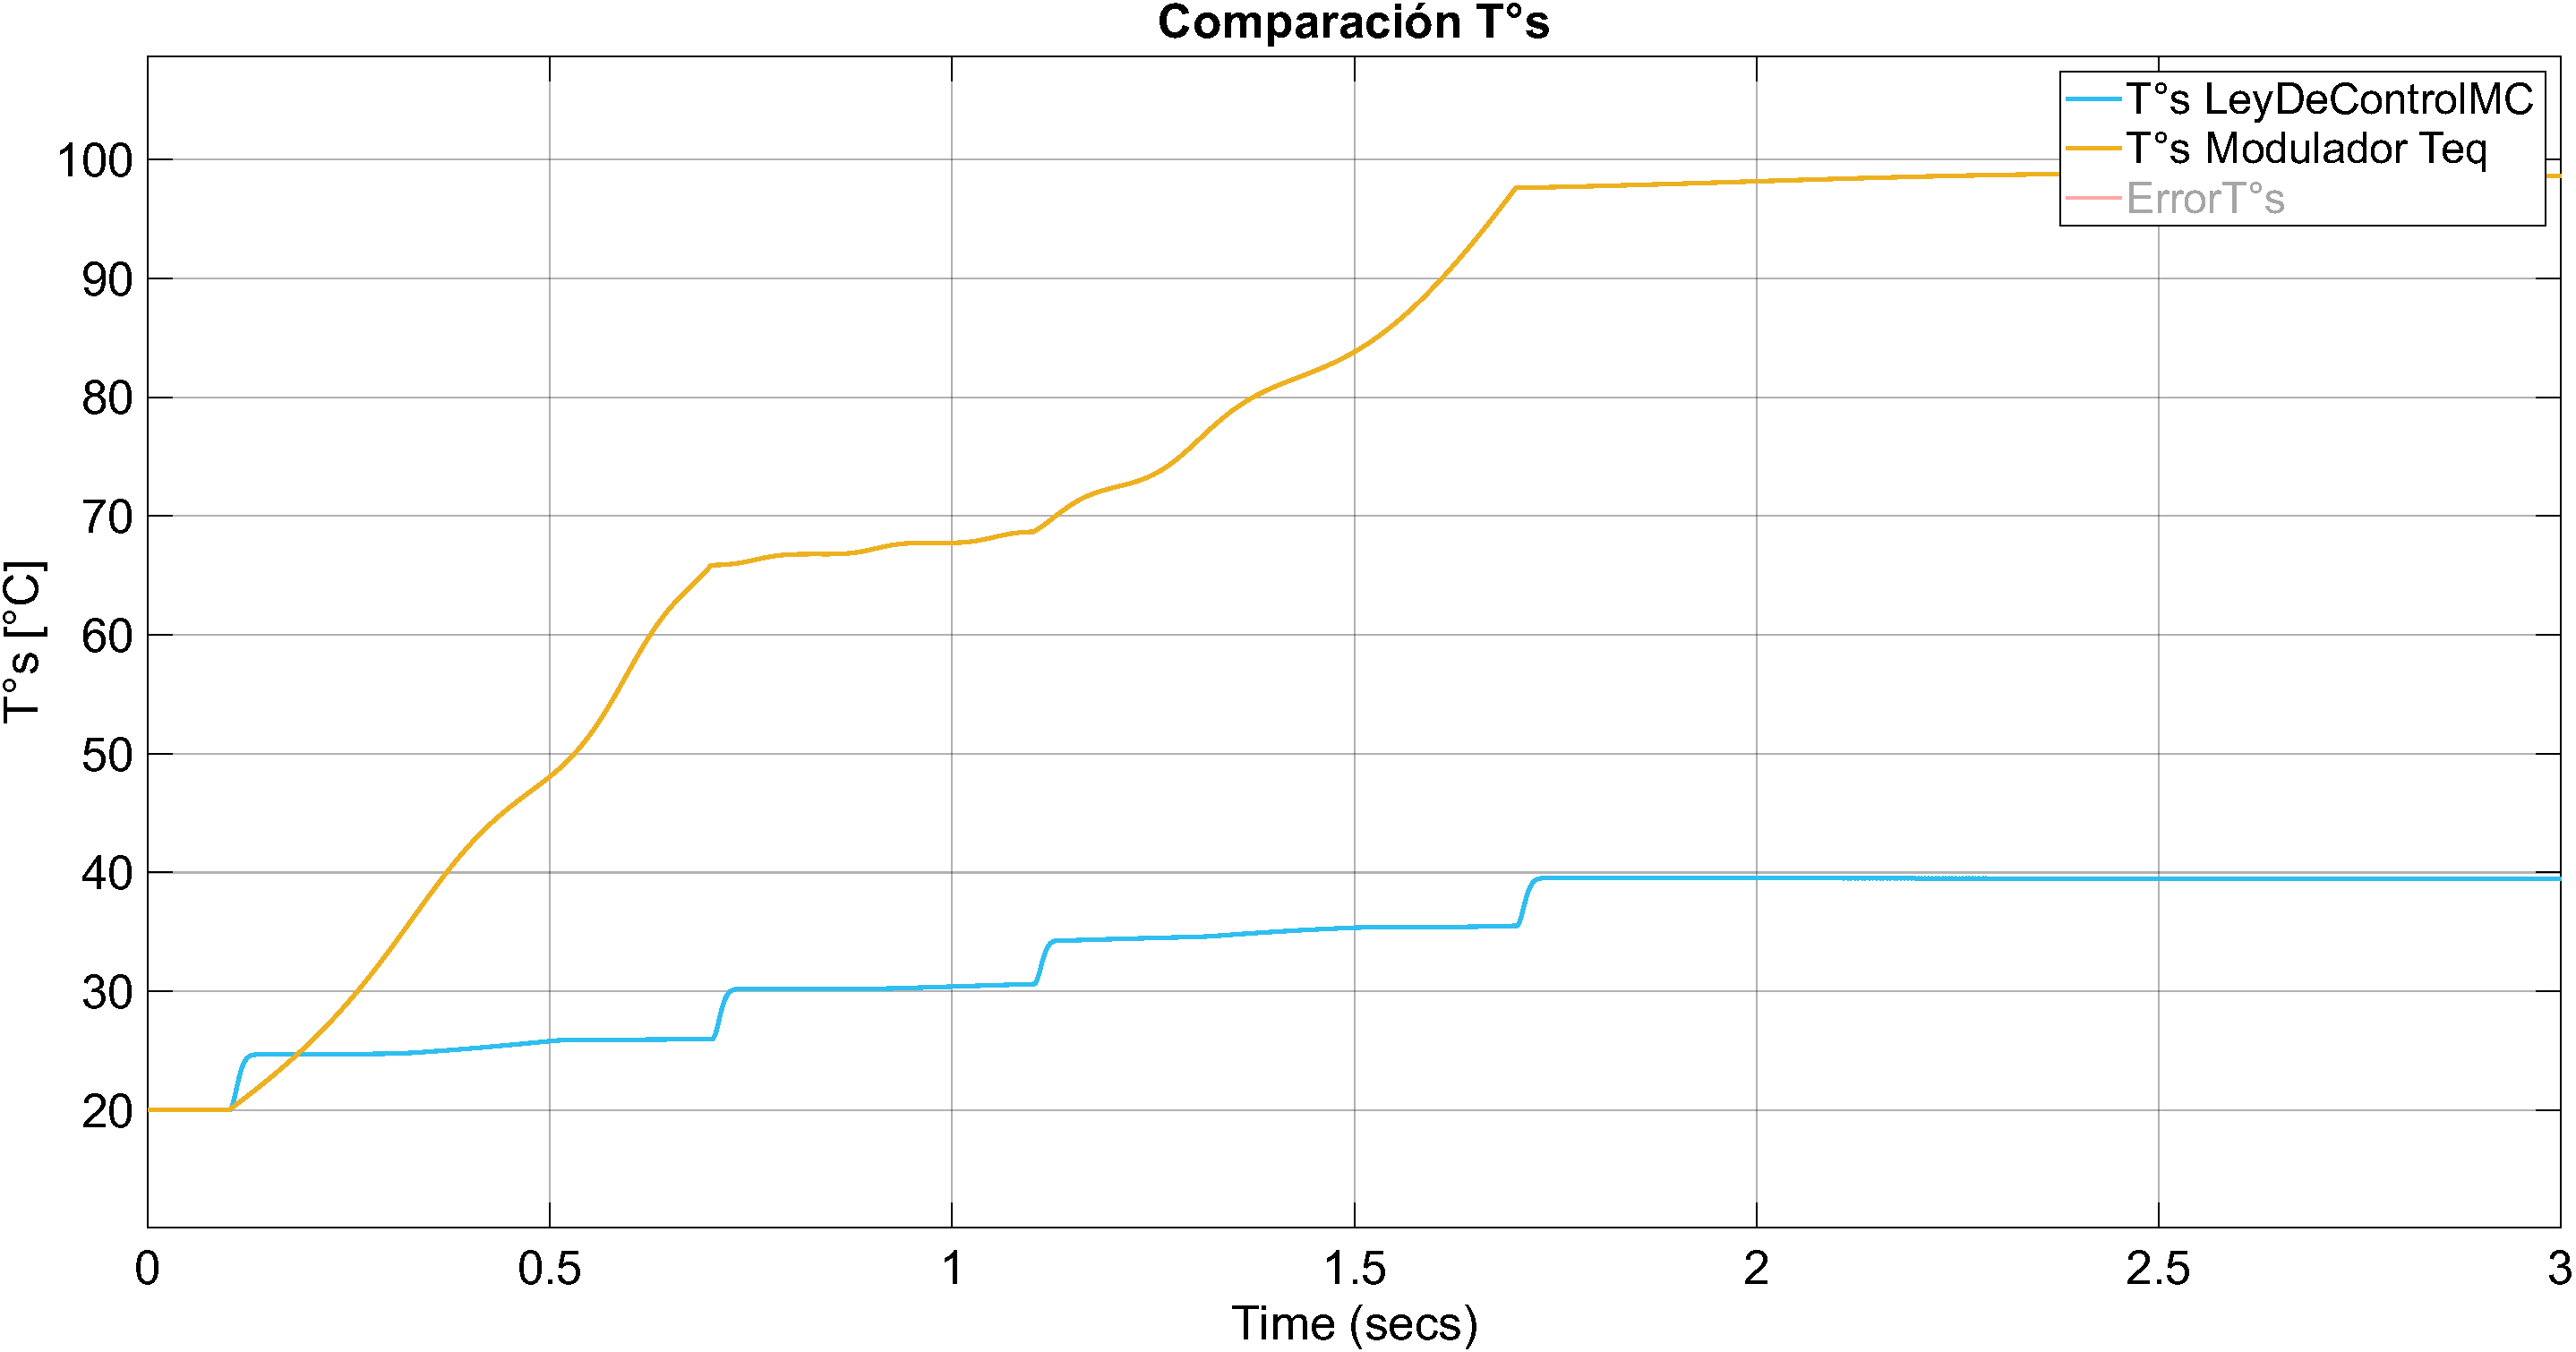
\includegraphics[width=0.95\linewidth]
        {attachments/Ts_LeyCMC_vs_ModTeq.pdf}
    \caption{Comparación de la temperatura del bobinado
    $T_s^\circ$ entre el modelo GNL con Ley de Control Mínima
    Complementaria y con Modulador de Torque Equivalente.}
    \label{fig:ts-leycmc-vs-modteq}
\end{figure}

La consigna escalonada de torque produce una evolución de la
velocidad angular $\omega_m$ aproximadamente trapezoidal,
predominantemente positiva durante el intervalo analizado.
Como la posición angular $\theta_m$ es la integral de la
velocidad, presenta tramos aproximadamente parabólicos cuando
la velocidad varía linealmente y tramos aproximadamente lineales
cuando esta se mantiene constante.

El torque electromagnético presenta variaciones asociadas a
las compensaciones mecánicas incorporadas por el Modulador
de Torque Equivalente. La compensación viscosa depende de
la velocidad angular, mientras que la compensación gravitatoria
depende de la posición de la carga mediante
$\sin(\theta_m/r)$. Por ello, aun durante los intervalos de
consigna de torque constante, el torque electromagnético
requerido puede variar a medida que evoluciona el movimiento.

Estas variaciones se reflejan en la corriente del eje de
cuadratura, responsable de la producción de torque cuando
$i_{ds}^{r}\approx 0$. Para interpretar su efecto térmico,
debe considerarse la integral del cuadrado de la corriente,
ponderada por la resistencia del bobinado. Con corrientes
directa y de secuencia cero despreciables, la energía disipada
por efecto Joule durante el intervalo $[t_0,t_f]$ es
aproximadamente:
\begin{equation}
    E_J \approx \frac{3}{2}
    \int_{t_0}^{t_f}
    R_s\!\left(T_s^\circ(t)\right)
    \left[i_{qs}^{r}(t)\right]^2\,dt.
\end{equation}

Por tanto, los valores elevados y las oscilaciones de corriente
pueden incrementar las pérdidas térmicas al aumentar su valor
cuadrático medio. Este efecto contribuye al mayor calentamiento
observado con el Modulador de Torque Equivalente en la
Figura~\ref{fig:ts-leycmc-vs-modteq}. La evolución de la
temperatura resulta del balance entre estas pérdidas y el
calor transferido al ambiente.

% ---------------------------------------------------------------------------- %
\subsection{Controlador externo de movimiento: posición y velocidad}

El controlador externo de movimiento se diseña para recibir consignas de posición o velocidad angular mediante el método de sintonía serie con acción integral. Se adoptan como parámetros de diseño $\zeta = 0.75$ y $\omega_{n}=800 \frac{rad}{seg}$, y se consideran los valores nominales de los parámetros de carga $J_{l}$ y $b_{l}$, sin incluir la incertidumbre de los datos.

La consigna de torque se genera mediante una ley PID que combina los errores de posición y velocidad con la integral del error de posición. En el dominio de Laplace $s$, se expresa como:
\begin{align}
T_{m}^{*}(s) & = K_{p}^{\text{mov}}e_{\theta}(s) + K_{d}^{\text{mov}}s e_{\theta}(s) + K_{i}^{\text{mov}} \frac{1}{s} e_{\theta}(s)
\notag \\
 & = \Big[  K_{p}^{\text{mov}} + sK_{d}^{\text{mov}} + \frac{1}{s}K_{i}^{\text{mov}} \Big] e_{\theta}(s)
\notag \\
 & = \Big[  K_{p}^{\text{mov}} + sK_{d}^{\text{mov}} + \frac{1}{s}K_{i}^{\text{mov}} \Big] \Big( \Theta^{*}_{m}(s) - \Theta_{m}(s) \Big) % crear referencia \tag o lo que sea
\label{eq:pid-movimiento}
\end{align}

La dinámica mecánica resultante de la compensación del modulador de torque equivalente se describe mediante:
\begin{equation}
\label{eq:mecanica-compensada}
\frac{d\omega_{m}(t)}{dt} = \frac{1}{J_{eq}} \Big[ T_{m}^{*}(t)- \frac{1}{r} T_{dl}(t) \Big]
\end{equation}

Con condiciones iniciales nulas, su transformación al dominio de Laplace $s$ permite escribir:
\begin{align*}
s\Omega_{m}(s)  & = \frac{1}{J_{eq}} \Big[ T_{m}^{*}(s)- \frac{1}{r} T_{dl}(s) \Big] \\ 
s^{2}\Theta_{m}(s)  & = \frac{1}{J_{eq}} \Big[ T_{m}^{*}(s)- \frac{1}{r} T_{dl}(s) \Big] \\
s^{2}J_{eq} \Theta_{m}(s)  & = T_{m}^{*}(s)- \frac{1}{r} T_{dl}(s) 
\end{align*}

Al sustituir la consigna de torque por la ley PID \eqref{eq:pid-movimiento}, %referencia a la expresión de consigna T*m
resulta:
\[
s^{2}J_{eq} \Theta_{m}(s) = \Big[  K_{p}^{\text{mov}} + sK_{d}^{\text{mov}} + \frac{1}{s}K_{i}^{\text{mov}} \Big] \Big( \Theta^{*}_{m}(s) - \Theta_{m}(s) \Big) - \frac{1}{r} T_{dl}(s) 
\]
Agrupando los términos que dependen del ángulo $\Theta_m(s)$, se obtiene:
\[
\Big[ s^{2}J_{eq} + sK_{d}^{\text{mov}} + K_{p}^{\text{mov}}  + \frac{1}{s}K_{i}^{\text{mov}} \Big] \Theta_{m}(s) = \Big[  K_{p}^{\text{mov}} + sK_{d}^{\text{mov}} + \frac{1}{s}K_{i}^{\text{mov}} \Big] \Theta^{*}_{m}(s) - \frac{1}{r} T_{dl}(s) 
\]

Para eliminar las potencias negativas de $s$, se multiplican ambos miembros de la igualdad por $s$:

\[
\Big[ s^{3}J_{eq} + s^{2}K_{d}^{\text{mov}} + sK_{p}^{\text{mov}}  + K_{i}^{\text{mov}} \Big] \Theta_{m}(s) = \Big[  s^{2}K_{d}^{\text{mov}} + sK_{p}^{\text{mov}} + K_{i}^{\text{mov}} \Big] \Theta^{*}_{m}(s) - \frac{s}{r} T_{dl}(s) 
\]

Finalmente, al despejar la posición angular, resulta:
\begin{equation}
\label{eq:respuesta-posicion-lc}
\Theta_{m}(s) = \frac{  s^{2}K_{d}^{\text{mov}} + sK_{p}^{\text{mov}} + K_{i}^{\text{mov}} }{ s^{3}J_{eq} + s^{2}K_{d}^{\text{mov}} + sK_{p}^{\text{mov}}  + K_{i}^{\text{mov}} } \Theta^{*}_{m}(s) - \frac{\frac{s}{r}}{ s^{3}J_{eq} + s^{2}K_{d}^{\text{mov}} + sK_{p}^{\text{mov}}  + K_{i}^{\text{mov}} } T_{dl}(s) 
\end{equation}

Esta relación permite distinguir la contribución de la consigna de posición $\Theta_{m}^{*}(s)$ y la del torque perturbador $T_{dl}(s)$ a la respuesta del ángulo motor $\Theta_{m}(s)$. Las funciones de transferencia correspondientes, considerando nula la otra entrada en cada caso, son:

\begin{align}
G_{\Theta^{*}_{m}}(s) & = \frac{\Theta_{m}(s)}{\Theta^{*}_{m}(s) }  = \frac{1}{J_{eq}} \frac{  s^{2}K_{d}^{\text{mov}} + sK_{p}^{\text{mov}} + K_{i}^{\text{mov}} }{ s^{3}+ s^{2}\frac{K_{d}^{\text{mov}}}{J_{eq}} + s\frac{K_{p}^{\text{mov}}}{J_{eq}}  + \frac{K_{i}^{\text{mov}}}{J_{eq}} }
\label{eq:transferencia-posicion-lc} \\
G_{T_{ld}}(s) & = \frac{\Theta_{m}(s)}{T_{dl}(s) } =  - \frac{1}{rJ_{eq}} \frac{s}{ s^{3}+ s^{2}\frac{K_{d}^{\text{mov}}}{J_{eq}} + s\frac{K_{p}^{\text{mov}}}{J_{eq}}  + \frac{K_{i}^{\text{mov}}}{J_{eq}} }
\label{eq:transferencia-perturbacion-lc}
\end{align}

Ambas funciones de transferencia comparten el siguiente polinomio característico:
\begin{equation}
\label{eq:polinomio-movimiento}
P(s) = s^{3}+ s^{2}\frac{K_{d}^{\text{mov}}}{J_{eq}} + s\frac{K_{p}^{\text{mov}}}{J_{eq}}  + \frac{K_{i}^{\text{mov}}}{J_{eq}}
\end{equation}

La asignación considera tres polos situados a una distancia de $800\;\frac{rad}{seg}$ del origen. Se elige un par de polos complejos conjugados definido por $\zeta=0.75$ y $\omega_{n}=800 \frac{rad}{seg}$, junto con un tercer polo real negativo cuyo módulo es $|p_{3}|=\omega_{n}=800 \frac{rad}{seg}$. El polinomio característico deseado resulta:

\begin{align}
P^{*}(s)  & = (s^{2}+2\zeta \omega_{n}s+\omega_{n}^{2})(s+\omega_{n})
\notag \\
P^{*}(s)  & = s^{3} + \omega_{n} (2\zeta+1) s^{2} + \omega_{n}^{2} (2\zeta+1)s + \omega_{n}^{3}
\label{eq:polinomio-deseado-movimiento}
\end{align}

Al igualar los coeficientes de los polinomios característicos \eqref{eq:polinomio-movimiento} y \eqref{eq:polinomio-deseado-movimiento} y despejar las ganancias, % tag a la expresión correcta
considerando la inercia equivalente $J_{eq}$ para la carga máxima $m_{l} =1.5\;[\text{kg}]$, se obtienen los siguientes valores:

\begin{equation}
\label{eq:ganancias-movimiento}
\begin{cases}
\omega_{n} (2\zeta+1) & = \frac{K_{d}^{\text{mov}}}{J_{eq}} \\
\omega_{n}^{2} (2\zeta+1) & = \frac{K_{p}^{\text{mov}}}{J_{eq}} \\
\omega_{n}^{3} & = \frac{K_{i}^{\text{mov}}}{J_{eq}}
\end{cases} \quad  \implies \quad 
\begin{cases}
 K_{d}^{\text{mov}} & = \omega_{n} (2\zeta+1){J_{eq}} = 0.0917 \; \mathrm{\frac{Nm}{rad/s}}\\
K_{p}^{\text{mov}} & = \omega_{n}^{2} (2\zeta+1) {J_{eq}} = 73.3222 \mathrm{\frac{Nm}{rad}}\\
K_{i}^{\text{mov}} & = \omega_{n}^{3}{J_{eq}} = 23463 \mathrm{\frac{Nm}{rad\cdot s}}
\end{cases}
\end{equation}


\begin{figure}[!htbp]
    \centering
    \begin{minipage}[c]{0.62\linewidth}
        \centering
        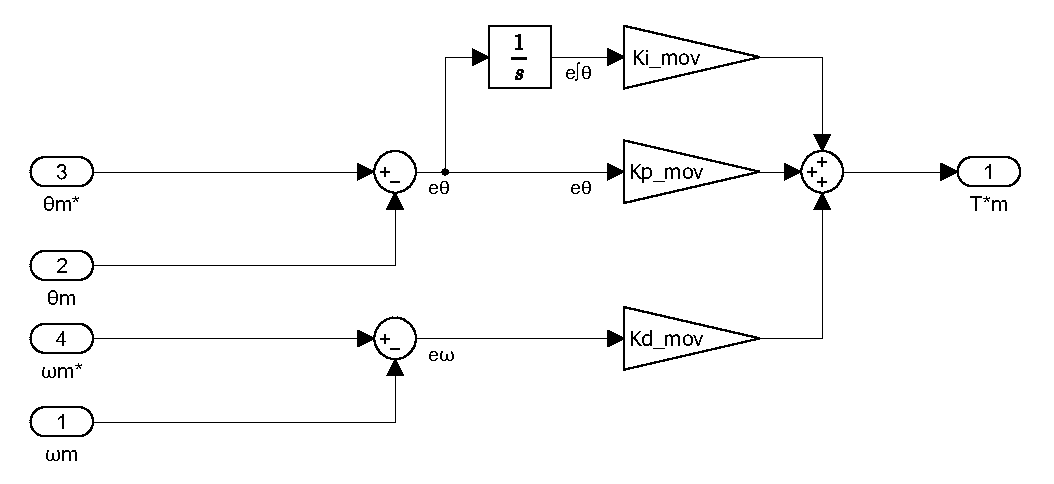
\includegraphics[width=\linewidth]{attachments/PID Movimiento.pdf}
    \end{minipage}
    \hfill
    \begin{minipage}[c]{0.33\linewidth}
        \centering
        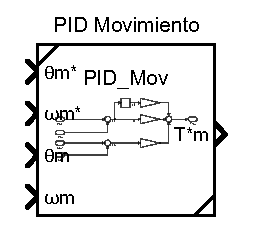
\includegraphics[width=\linewidth]{attachments/Bloque PID Movimiento.pdf}
    \end{minipage}
    \caption{Controlador PID de movimiento: diagrama interno y bloque
    de implementación, con entradas de referencia $\theta_m^*$ y
    $\omega_m^*$, posición medida $\theta'_m$ y velocidad estimada
    $\hat{\omega}_m$.}
    \label{fig:PIDMovimiento}
\end{figure}

La variación de la masa de carga modifica la inercia equivalente
referida al eje motor y, por consiguiente, la ubicación de los
polos del lazo cerrado de movimiento. Para evaluar este efecto,
se mantienen fijas las ganancias calculadas para la carga máxima
$m_l=1.5\;\mathrm{kg}$:
\[
K_d^{\mathrm{mov}}\approx 0.0917\;\mathrm{\frac{N\,m\,s}{rad}},
\qquad
K_p^{\mathrm{mov}}\approx 73.3222\;\mathrm{\frac{N\,m}{rad}},
\qquad
K_i^{\mathrm{mov}}\approx 23463\;\mathrm{\frac{N\,m}{rad\,s}}.
\]

La dependencia de la inercia equivalente con la masa resulta:
\begin{equation}
    J_{eq}(m_l)
    = J_m+\frac{J_{l,\min}+m_l l_l^2}{r^2}
    = J_m+\frac{J_{l,\min}}{r^2}
      +\frac{l_l^2}{r^2}m_l.
\end{equation}
Por tanto, $J_{eq}$ presenta una dependencia afín con $m_l$,
debido a la contribución constante de la inercia del motor
y de la carga sin masa útil. Para los parámetros considerados,
varía aproximadamente entre
$19.78\times10^{-6}\;\mathrm{kg\,m^2}$ y
$45.83\times10^{-6}\;\mathrm{kg\,m^2}$.

El barrido se realiza variando $m_l$ entre $0$ y
$1.5\;\mathrm{kg}$, sin recalcular las ganancias del controlador.
Para cada valor se determinan las raíces del polinomio
característico:
\begin{equation}
    P(s;m_l)
    = s^3
    +\frac{K_d^{\mathrm{mov}}}{J_{eq}(m_l)}s^2
    +\frac{K_p^{\mathrm{mov}}}{J_{eq}(m_l)}s
    +\frac{K_i^{\mathrm{mov}}}{J_{eq}(m_l)}.
\end{equation}

La Figura~\ref{fig:migracion-polos-masa} muestra la migración
de los polos obtenida. Para la masa máxima se recuperan los
polos de diseño $-800$ y $-600\pm j529.15\;\mathrm{s^{-1}}$.
Al disminuir la masa, aumenta el cociente entre cada ganancia
fija y la inercia equivalente, modificando la dinámica del
lazo cerrado. El desplazamiento de los polos no es proporcional
a la masa, ya que su ubicación resulta de las raíces del
polinomio característico.

Este análisis corresponde al modelo mecánico ideal compensado,
bajo las hipótesis de seguimiento ideal de corriente y
compensación mecánica exacta.

\begin{figure}[!htbp]
    \centering
    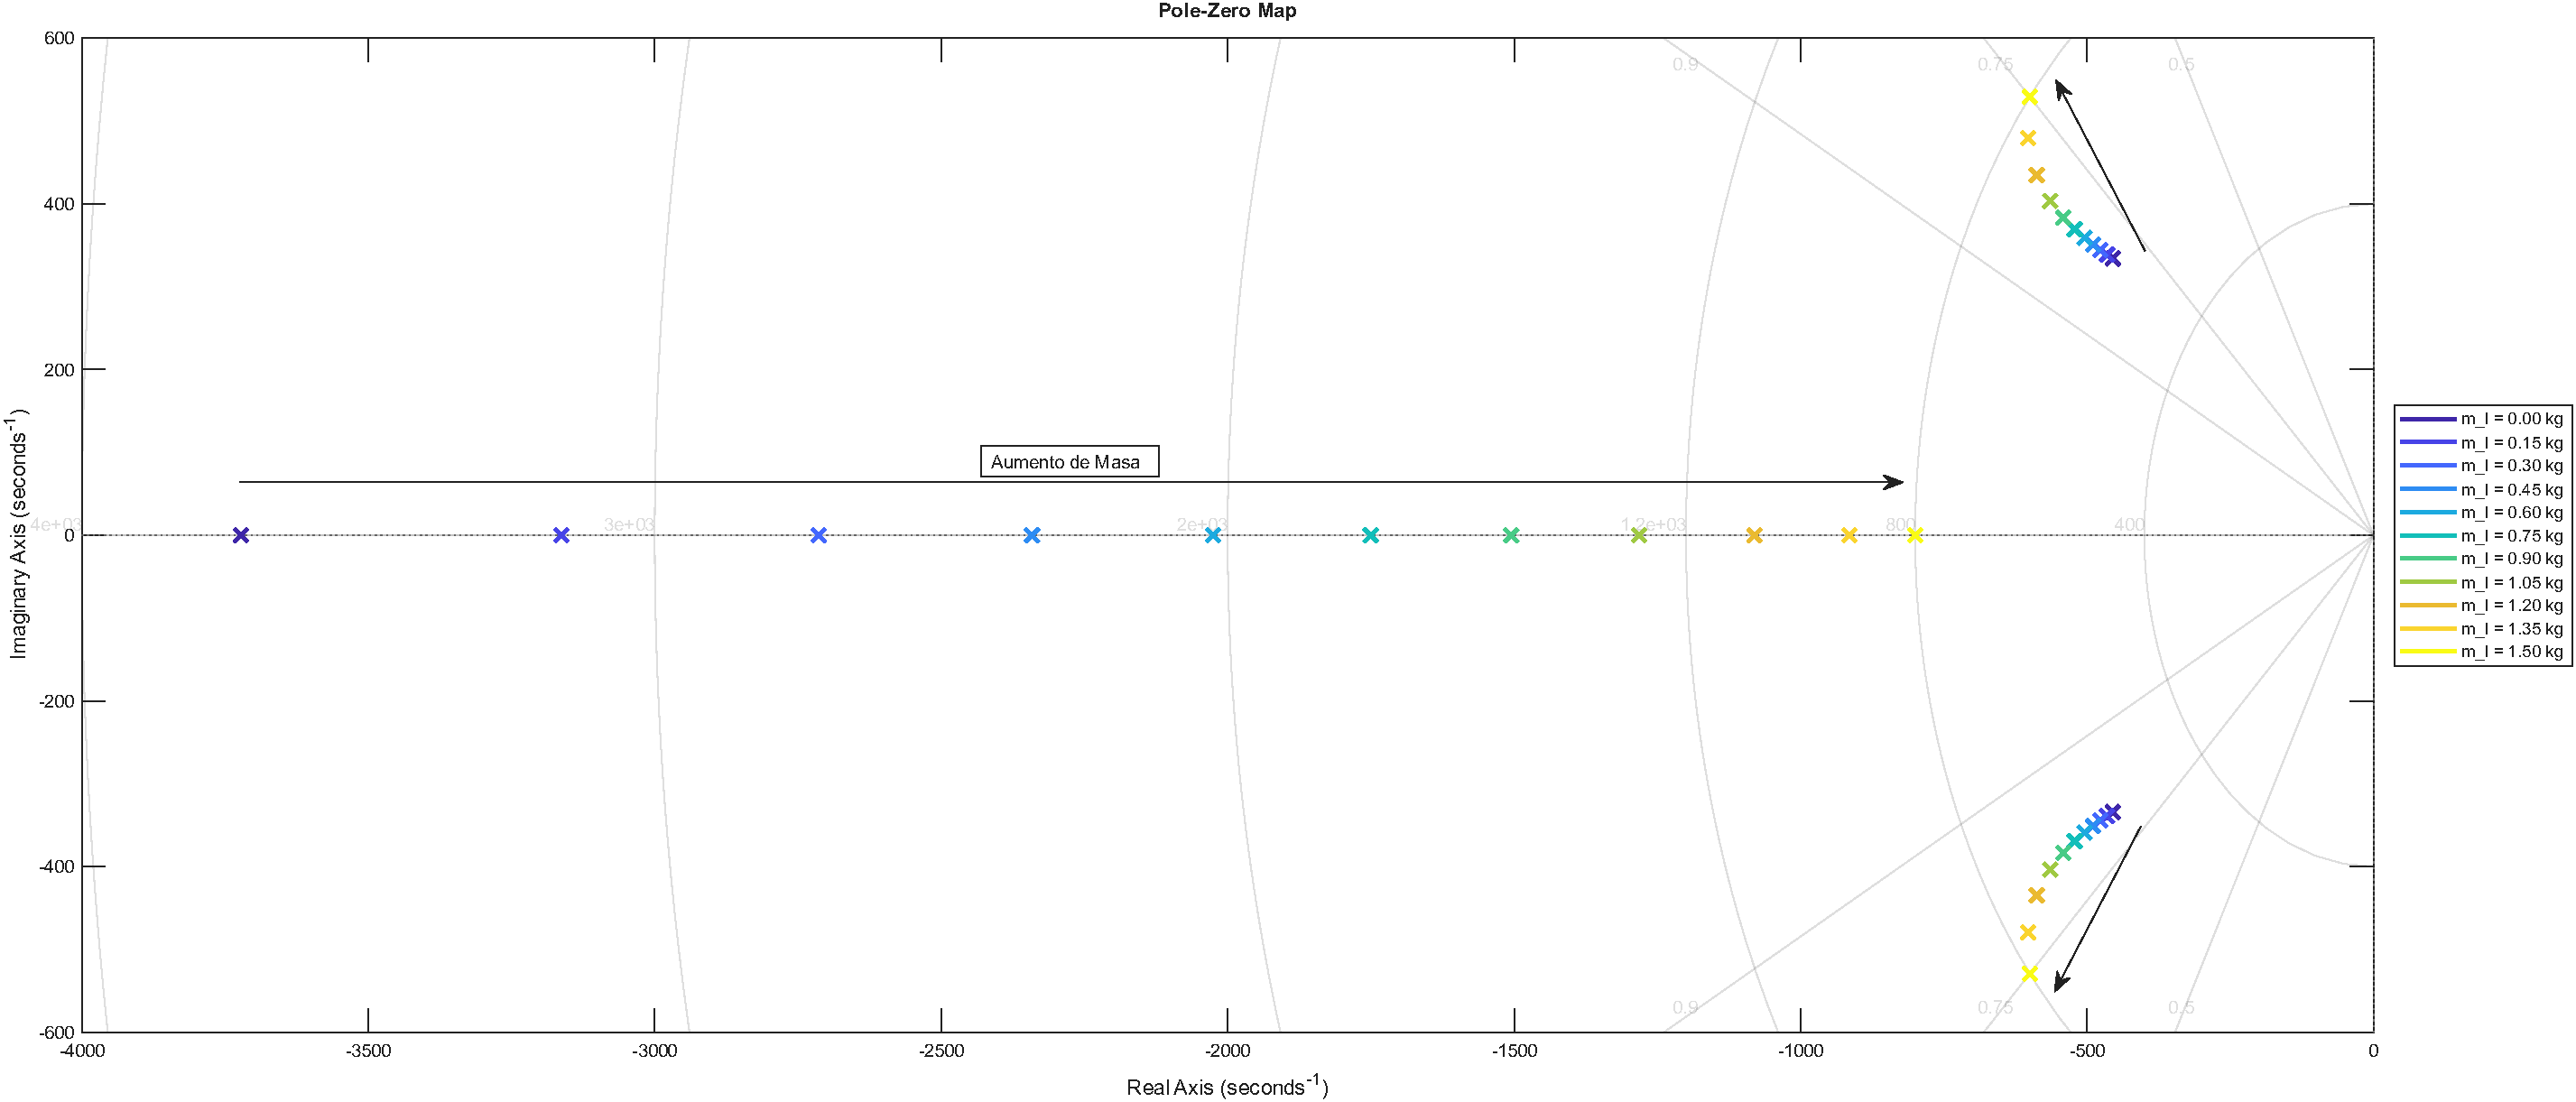
\includegraphics[width=0.95\linewidth]
        {attachments/Migracion de polos por variacion de masa.pdf}
    \caption{Migración de los polos del lazo cerrado ideal de
    movimiento al variar la masa de carga entre $0$ y
    $1.5\;\mathrm{kg}$, manteniendo fijas las ganancias
    calculadas para la carga máxima.}
    \label{fig:migracion-polos-masa}
\end{figure}

\begin{table}[!htbp]

    \centering

\small

\caption{Polos del lazo cerrado ideal de movimiento al variar la masa, con ganancias fijas calculadas para $m_1=1.50\;\mathrm{kg}$.}

\label{tab:polos-barrido-masa}

\begin{tabular}{c c c c c c c}
\hline
$m_l$ & $p_1$ & $p_{2,3}$ & $\omega_n$ & $\omega_d$ & $\zeta$ & $\tau$ \\

$[\mathrm{kg} ]$ & $[\mathrm{s^{-1}}]$ & $[\mathrm{s^{-1}}]$ & $[\mathrm{rad/s}]$ & $[\mathrm{rad/s}]$ & $[\mathrm{adim}]$ & $[\mathrm{ms}]$ \\

\hline

0.00 & $-3722.52$ & $-454.99 \pm j334.01$ & 564.43 & 334.01 & 0.8061 & 2.198 \\
0.15 & $-3163.04$ & $-465.31 \pm j338.83$ & 575.60 & 338.83 & 0.8084 & 2.149 \\
0.30 & $-2713.47$ & $-476.83 \pm j344.39$ & 588.19 & 344.39 & 0.8107 & 2.097 \\
0.45 & $-2341.46$ & $-489.82 \pm j350.98$ & 602.58 & 350.98 & 0.8129 & 2.042 \\
0.60 & $-2025.46$ & $-504.63 \pm j359.04$ & 619.32 & 359.04 & 0.8148 & 1.982 \\
0.75 & $-1750.34$ & $-521.74 \pm j369.33$ & 639.23 & 369.33 & 0.8162 & 1.917 \\
0.90 & $-1505.06$ & $-541.65 \pm j383.25$ & 663.52 & 383.25 & 0.8163 & 1.846 \\
1.05 & $-1282.09$ & $-564.47 \pm j403.48$ & 693.84 & 403.48 & 0.8135 & 1.772 \\
1.20 & $-1080.68$ & $-587.89 \pm j434.64$ & 731.11 & 434.64 & 0.8041 & 1.701 \\
1.35 & $-914.75$ & $-602.88 \pm j479.56$ & 770.35 & 479.56 & 0.7826 & 1.659 \\
1.50 & $-800.00$ & $-600.00 \pm j529.15$ & 800.00 & 529.15 & 0.7500 & 1.667 \\

\hline
\end{tabular}
\end{table}

Los resultados de la Tabla~\ref{tab:polos-barrido-masa} muestran
que, con las ganancias mantenidas constantes, la variación de
masa modifica de manera diferente el polo real y el par complejo
conjugado. Para la carga máxima se recupera la ubicación de polos
adoptada en el diseño, con $\zeta=0.75$ y
$\omega_n=800\;\mathrm{rad/s}$.

Al disminuir la masa de carga, el polo real se desplaza hacia
valores más negativos, por lo que su contribución al transitorio
se atenúa más rápidamente. Sin embargo, al comparar los extremos
del barrido, el par complejo se aproxima al origen: su parte real
pasa de $-600$ a aproximadamente $-454.99\;\mathrm{s^{-1}}$ y su
frecuencia de oscilación disminuye de $529.15$ a
$334.01\;\mathrm{rad/s}$.

La constante de tiempo de la envolvente asociada al par complejo,
definida como $\tau=1/|\operatorname{Re}(p_{2,3})|$, aumenta de
$1.667$ a $2.198\;\mathrm{ms}$, aproximadamente un $32\%$.
Esto indica una atenuación más lenta de este modo. A su vez,
el coeficiente de amortiguamiento aumenta de $0.75$ a
aproximadamente $0.806$, por lo que el par presenta una menor
tendencia oscilatoria. Estas propiedades no varían de forma
estrictamente monótona en todo el intervalo de masas.

Por tanto, el desplazamiento del polo real hacia la izquierda
no implica que la respuesta completa sea más rápida. El par
complejo conserva la dinámica de decaimiento más lenta y puede
dominar el establecimiento de la respuesta, dependiendo de su
participación en la salida.

Todos los polos permanecen en el semiplano izquierdo durante
el barrido, lo que indica estabilidad del modelo ideal analizado.


Finalmente, se presentan los polos del sistema bajo régimen de carga máxima y considerando el Modulador de Torque Equivalente:

\begin{figure}[!htbp]
    \centering
    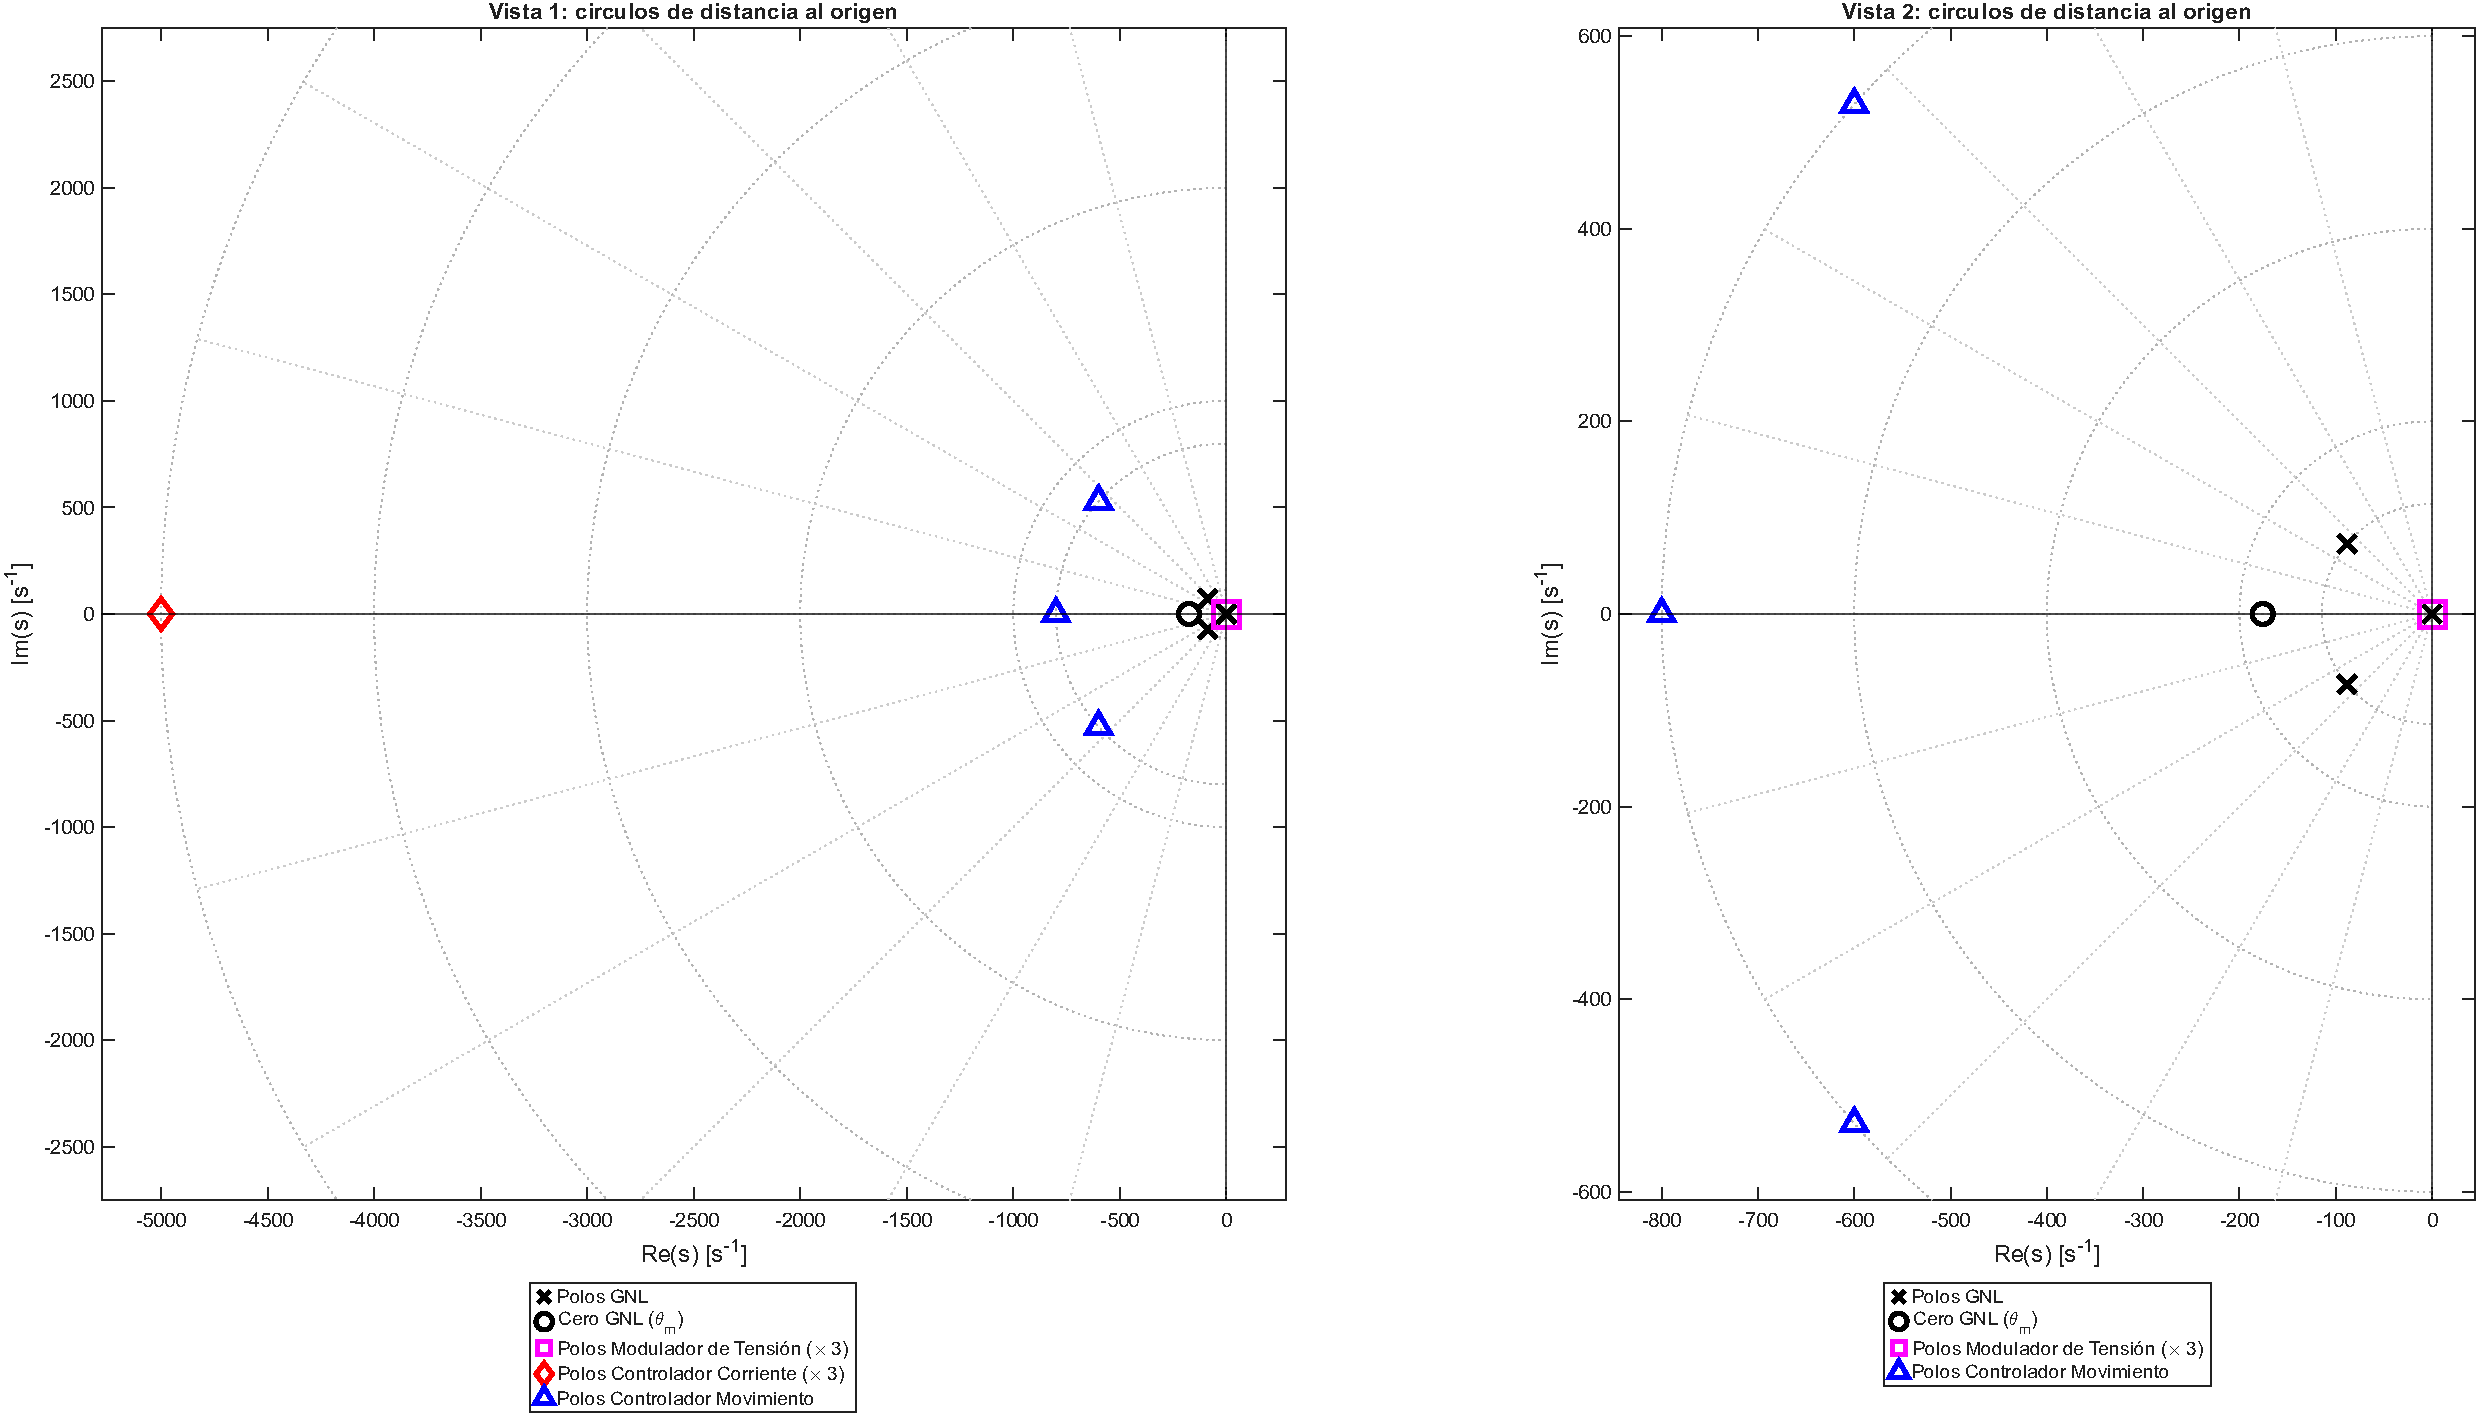
\includegraphics[width=0.95\linewidth]
        {attachments/Polos y ceros por grupo.pdf}
    \caption{Comparación de los polos y ceros de la planta LTI
    equivalente al modelo GNL y de los polos ideales del
    modulador de tensión, los lazos de corriente y el lazo
    cerrado de movimiento. Se presentan una vista general
    y una ampliación de la región próxima al origen.
    Las circunferencias indican distancias constantes al
    origen en el plano complejo $s$.}
    \label{fig:polos-ceros-por-grupo}
\end{figure}


% [TODO] Insertar imagen del bloque de Simulink

% ---------------------------------------------------------------------------- %
\subsection{Incorporación y diseño del observador de estado de orden reducido}\label{subsec:observador de estado de orden reducido}

El observador se diseña a partir de las dinámicas de la posición angular $\theta_{m}$ y la velocidad angular $\omega_{m}$ del motor, considerando las compensaciones por realimentación no lineal introducidas en el modulador de torque. La posición angular es la salida medida del subsistema mecánico, cuyo modelo se expresa como:

\[
\left\{
\begin{aligned}
\frac{d \theta_{m}(t) }{dt} & = \omega_{m}(t) \\
\frac{d \omega_{m}(t) }{dt} & = \frac{1}{J_{eq}} \Big[ T_{m}^{*}(t)-\frac{1}{r}T_{dl}(t) \Big] \\
y & = \begin{bmatrix} 1 & 0 \end{bmatrix} \begin{bmatrix} \theta_{m}(t) \\ \omega_{m}(t) \end{bmatrix}
\end{aligned}
\right.
\]
La representación matricial correspondiente es:
\begin{equation}
\label{eq:planta-observador}
\left\{
\begin{aligned}
\begin{bmatrix} \frac{d \theta_{m}(t) }{dt} \\ \frac{d \omega_{m}(t) }{dt}  \end{bmatrix} 
 & = \begin{bmatrix} 0 & 1 \\0 & 0 \end{bmatrix} \begin{bmatrix} \theta_{m}(t) \\ \omega_{m}(t) \end{bmatrix} + \begin{bmatrix} 0 & 0 \\ \frac{1}{J_{eq}} & -\frac{1}{rJ_{eq}} \end{bmatrix} \begin{bmatrix} T^{*}_{m}(t) \\ T_{dl}(t) \end{bmatrix} \\
y & = \begin{bmatrix} 1 & 0 \end{bmatrix} \begin{bmatrix} \theta_{m}(t) \\ \omega_{m}(t) \end{bmatrix}
\end{aligned}
\right.
\end{equation}

Para construir el observador, se parte de la siguiente estructura matricial, que incorpora una corrección proporcional al error entre la salida medida y la estimada:

\begin{equation}
\label{eq:estructura-observador}
\left\{
\begin{aligned}
\frac{d \mathbf{\hat{x}}(t) }{dt} & = \mathbf{A} \mathbf{\hat{x}}(t) + \mathbf{B}\mathbf{u}(t) + \mathbf{L}(\mathbf{y}-\mathbf{C}\mathbf{\hat{x}}) \\
\mathbf{\hat{y}} & = \mathbf{C} \mathbf{\hat{x}}
\end{aligned}
\right.
\end{equation}

A partir del modelo del subsistema mecánico definido por $\theta_{m}$ y $\omega_{m}$, se identifican las matrices:
\[
\mathbf{A}=\begin{bmatrix} 0 & 1 \\0 & 0 \end{bmatrix}
\]
\[
\mathbf{B} = \begin{bmatrix} 0 & 0 \\ \frac{1}{J_{eq}} & -\frac{1}{rJ_{eq}} \end{bmatrix}
\]
\[
\mathbf{C}=\begin{bmatrix} 1 & 0\end{bmatrix}
\]
La matriz de ganancias del observador debe tener dimensiones compatibles con el término de corrección:
\begin{equation}
\label{eq:ganancias-observador-vector}
\mathbf{A}-\mathbf{L}\mathbf{C} \in \mathbb{R}^{2\times2} \implies \mathbf{L} \in \mathbb{R}^{2\times1}, \qquad \mathbf{L}=\begin{bmatrix} K_{\theta} \\ K_{\omega} \end{bmatrix}
\end{equation}

Teniendo en cuenta que el torque de perturbación de carga mecánica $T_{dl}(t)$ es una entrada de perturbación y no es posible introducirla al modelo del observador de estado de orden reducido debido a su naturaleza impredecible desde la perspectiva de control, se sustituye las matrices previamente definidas al modelo observador \eqref{eq:estructura-observador}, con la modificación $\mathbf{B_u}=\begin{bmatrix} 0 \\ \frac{1}{J_eq} \end{bmatrix}$, llagandose a las ecuaciones:
\begin{equation}
\label{eq:observador-mecanico}
\left\{
\begin{aligned}
\begin{bmatrix} \frac{d \hat{\theta}_{m}(t) }{dt} \\ \frac{d \hat{\omega}_{m}(t) }{dt}  \end{bmatrix} 
 & = \begin{bmatrix} 0 & 1 \\0 & 0 \end{bmatrix} \begin{bmatrix} \hat{\theta}_{m}(t) \\ \hat{\omega}_{m}(t) \end{bmatrix} + \begin{bmatrix} 0 \\ \frac{1}{J_{eq}} \end{bmatrix} T^{*}_{m}(t) + \begin{bmatrix} K_{\theta} \\ K_{\omega} \end{bmatrix} \Bigg( \theta_{m}(t) - \begin{bmatrix} 1 & 0 \end{bmatrix} \begin{bmatrix} \hat{\theta}_{m}(t) \\ \hat{\omega}_{m}(t) \end{bmatrix} \Bigg) \\
\hat{y} & = \begin{bmatrix} 1 & 0 \end{bmatrix} \begin{bmatrix} \hat{\theta}_{m}(t) \\ \hat{\omega}_{m}(t) \end{bmatrix}
\end{aligned}
\right.
\end{equation}

Se define el error de estimación como $\mathbf{\tilde{x}}=\mathbf{x}-\mathbf{\hat{x}}$ y se utiliza la relación $\mathbf{y} = \mathbf{C}\mathbf{x}$. Al restar las ecuaciones del observador \eqref{eq:observador-mecanico} % hacer referencia a la ecuación del modelo reducido de la planta
de las ecuaciones de la planta \eqref{eq:planta-observador}, % hacer referencia a la ecuación del modelo del observador de estado
se obtiene el siguiente modelo del error:

\begin{equation}
\label{eq:error-observador}
\left\{
\begin{aligned}
\begin{bmatrix} \frac{d \tilde{\theta}_{m}(t) }{dt} \\ \frac{d \tilde{\omega}_{m}(t) }{dt}  \end{bmatrix} 
 & = \begin{bmatrix} 0 & 1 \\0 & 0 \end{bmatrix} \begin{bmatrix} \tilde{\theta}_{m}(t) \\ \tilde{\omega}_{m}(t) \end{bmatrix} - \begin{bmatrix} K_{\theta} \\ K_{\omega} \end{bmatrix} \begin{bmatrix} 1 & 0 \end{bmatrix} \begin{bmatrix} \tilde{\theta}_{m}(t) \\ \tilde{\omega}_{m}(t) \end{bmatrix} + \begin{bmatrix} 0 \\ \frac{1}{rJ_{eq}} \end{bmatrix} T_{dl}(t) \\
\tilde{y} & = \begin{bmatrix} 1 & 0 \end{bmatrix} \begin{bmatrix} \tilde{\theta}_{m}(t) \\ \tilde{\omega}_{m}(t) \end{bmatrix}
\end{aligned}
\right.
\end{equation}

La matriz de estado que gobierna la dinámica del error de estimación es:

\begin{equation}
\label{eq:matriz-error-observador}
\mathbf{A}_{\text{obs}} = \mathbf{A}-\mathbf{L}\mathbf{C} = \begin{bmatrix}
-K_{\theta} & 1 \\
-K_{\omega} & 0
\end{bmatrix}
\end{equation}

Para analizar la estabilidad de \eqref{eq:error-observador}, se calcula el polinomio característico de $\mathbf{A}_{\text{obs}}$:

\begin{equation}
\label{eq:polinomio-observador}
\begin{aligned}
\det(s\mathbf{I}-\mathbf{A}_{\text{obs}}) &  = \Bigg| \begin{matrix}
s+K_{\theta} & -1 \\
K_{\omega} & s
\end{matrix} \Bigg|  \\
 & = (s+K_{\theta})(s)+K_{\omega} \\
 & = s^{2}+K_{\theta}s+K_{\omega}
\end{aligned}
\end{equation}

El criterio de diseño fija dos polos coincidentes para el observador, con módulos $|p_{\text{obs,1}}|=|p_{\text{obs,2}}|=3200\;\frac{rad}{seg}$. El polinomio deseado se plantea como:

\begin{equation}
\label{eq:polinomio-deseado-observador}
P^{*}_{\text{obs}}(s) = (s+p_{\text{obs}})^{2}=s^{2}+2p_{\text{obs}}s+p_{\text{obs}}^{2}
\end{equation}

Al comparar los coeficientes de \eqref{eq:polinomio-deseado-observador} con los del polinomio del error de estimación \eqref{eq:polinomio-observador}, se determinan las ganancias:
\begin{equation}
\label{eq:ganancias-observador}
\left\{
\begin{aligned}
K_{\theta}   = 2p_{\text{obs}} & = 6\; 400 \; [\text{s}^{-1}] \\
K_{\omega}  = p_{\text{obs}}^{2} & = 10\; 240\; 000 \; [\text{s}^{-2}]
\end{aligned}
\right.
\end{equation}


\begin{figure}[!htbp]
    \centering
    \begin{adjustbox}{max totalsize={\linewidth}{0.65\textheight},center}
        \begin{minipage}{\linewidth}
            \centering
            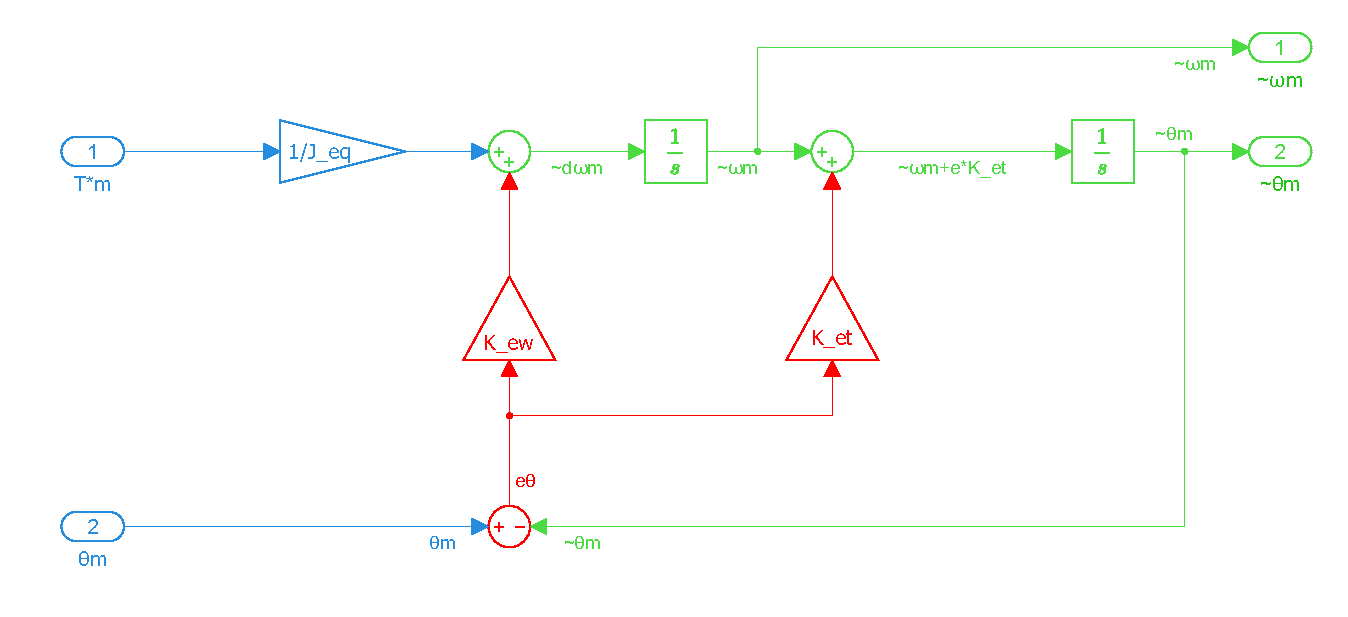
\includegraphics[width=\linewidth]{attachments/Estimador de Estado de Orden Reducido.pdf}
            \par\vspace{4mm}
            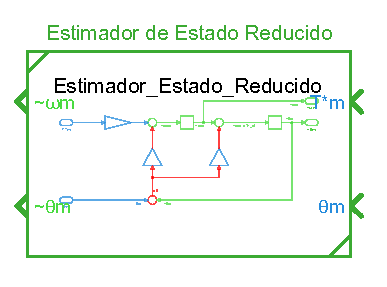
\includegraphics[width=0.42\linewidth,height=0.19\textheight,keepaspectratio]{attachments/Bloque Estimador de Estado de Orden Reducido.pdf}
        \end{minipage}
    \end{adjustbox}
    \caption{Bloque de estimador de estado reducido, con ganancias en el error de ángulo motor y estimación del ángulo motor.}
    \label{fig:EstimadorEstadoReducido}
\end{figure}

% [End 10/11/2026]
% ---------------------------------------------------------------------------- %
\subsection{ Simulación en tiempo continuo con modelo completo NL}
\subsubsection{Seguimiento de consigna de movimiento}
\label{subsubsec:seguimiento consigna movimiento}
Se analizará el comportamiento del modelo con y sin estimación debido a la siguiente consigna de movimiento. El análisis se hará teniendo en cuenta una masa de carga $m_l=0,5kg$ y una temperatura ambiente $T_{amb}=20^\circ C$
\begin{figure}[!htbp]
    \centering
    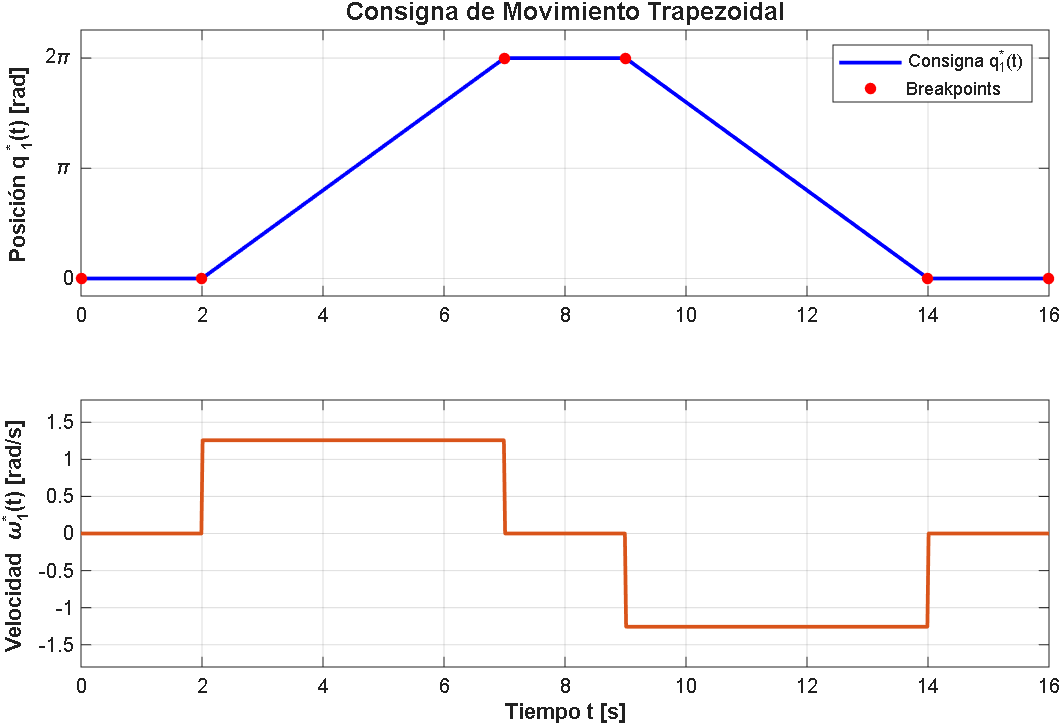
\includegraphics[width=0.75\linewidth]{attachments/consigna movimiento posición.png}
    \caption{Referencias de posición y velocidad de la carga para la consigna trapezoidal.}
    \label{fig:cosigna posicion}
\end{figure}
A continuación vemos la comparación con y sin estimación de $\theta_m$, $\omega_m$,$T_m$, $T^\circ_s$, $i_{qs}^r$, $i_{ds}^r$ y $i_{0s}^r$
\begin{figure}[!htbp]
    \centering
    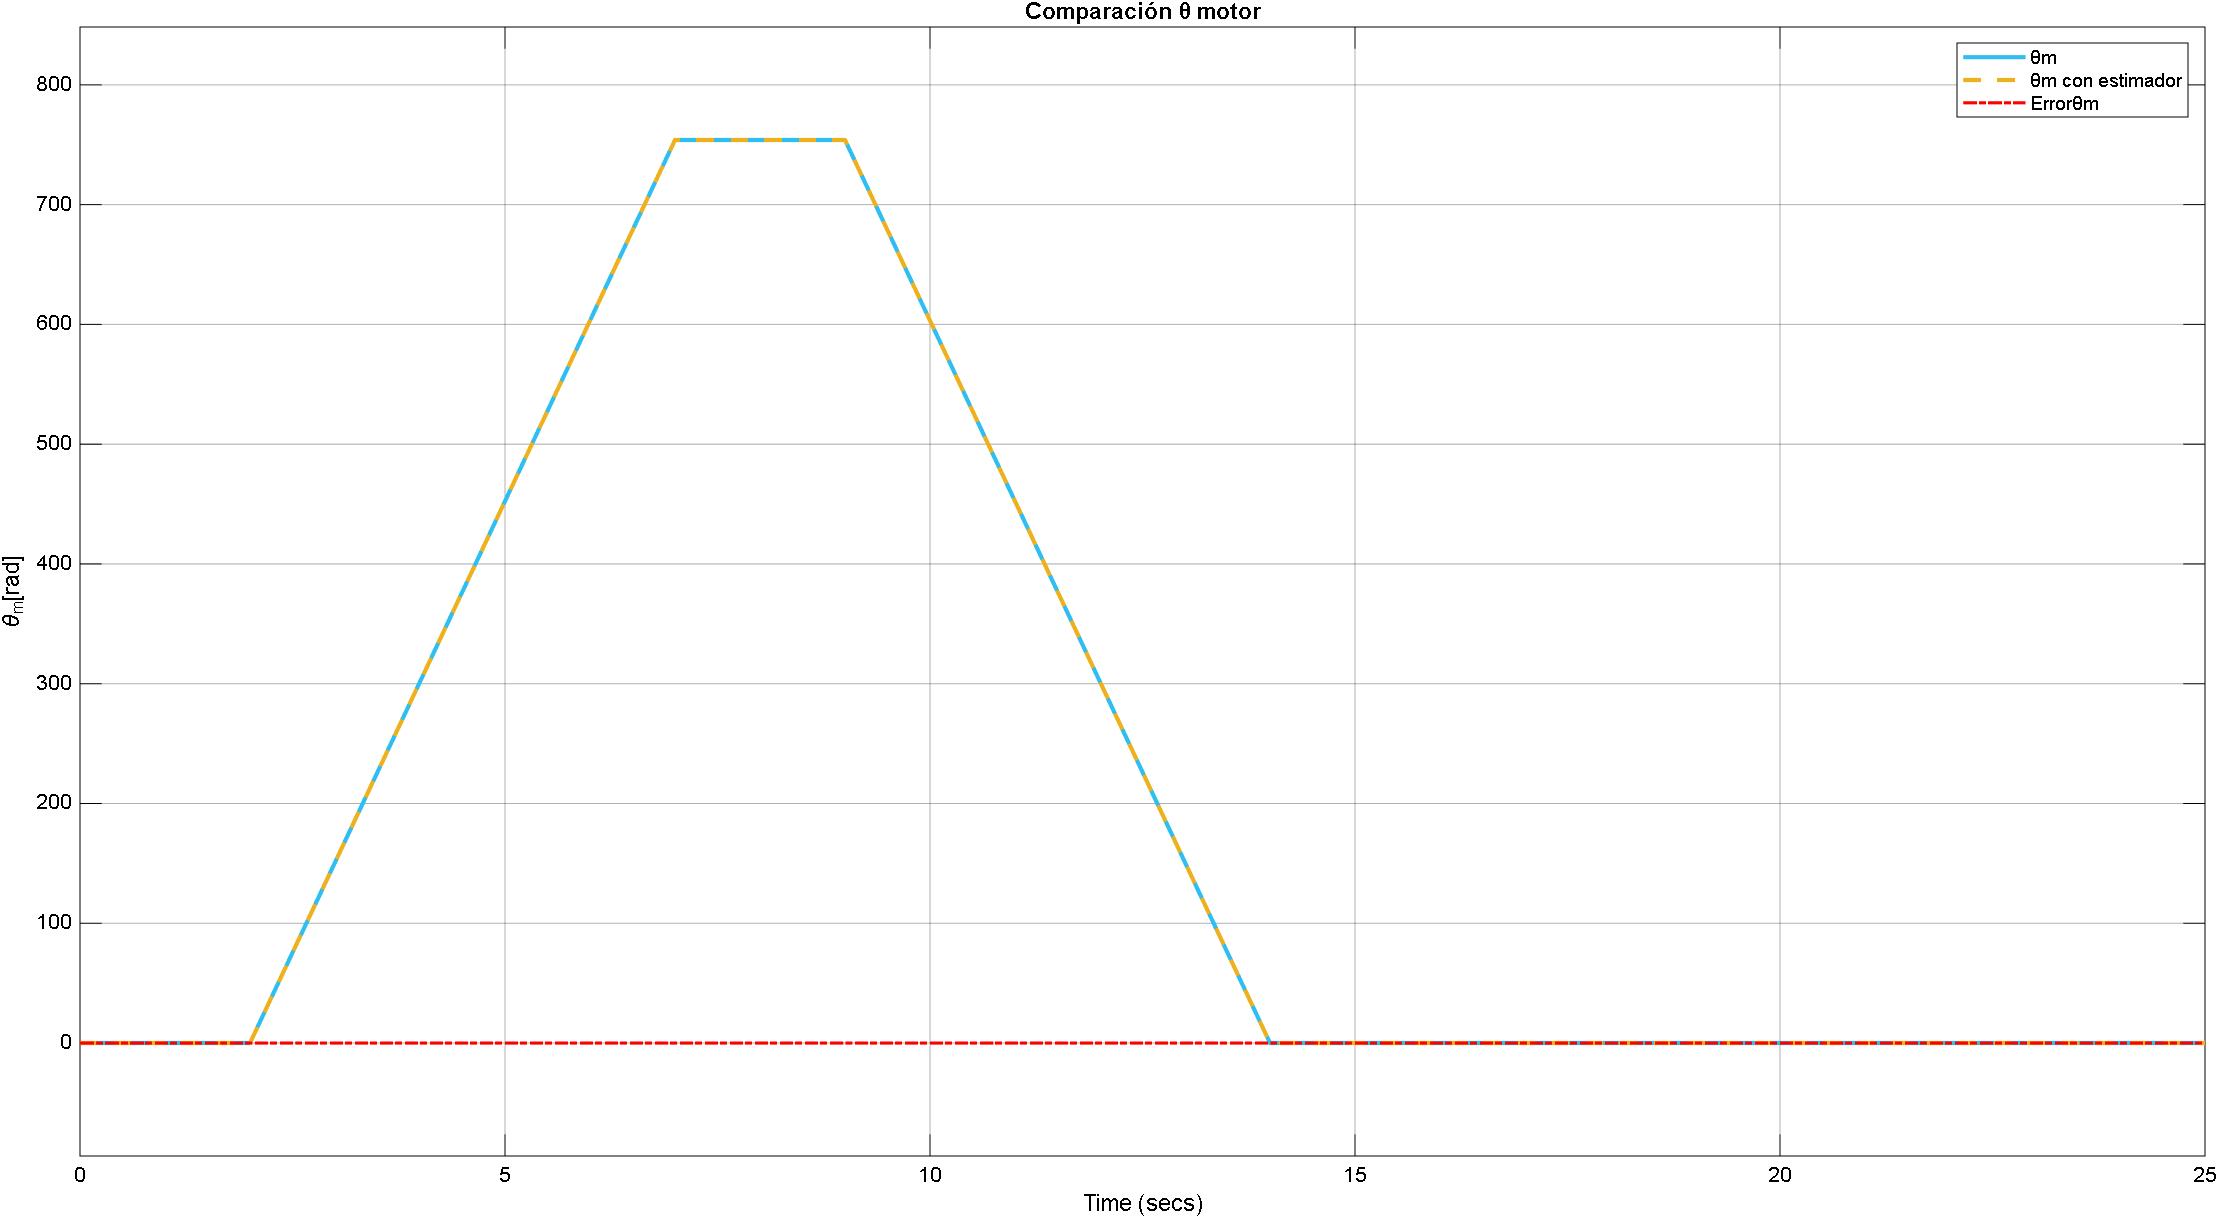
\includegraphics[width=0.86\linewidth,height=0.40\textheight,keepaspectratio]{attachments/comparacion estimacion posicion angulan.png}
    \caption{Comparación de $\theta_m$ entre los modelos con y sin estimación }
    \label{fig:comparacion estimación posicion angular}
\end{figure}
\begin{figure}[!htbp]
    \centering
    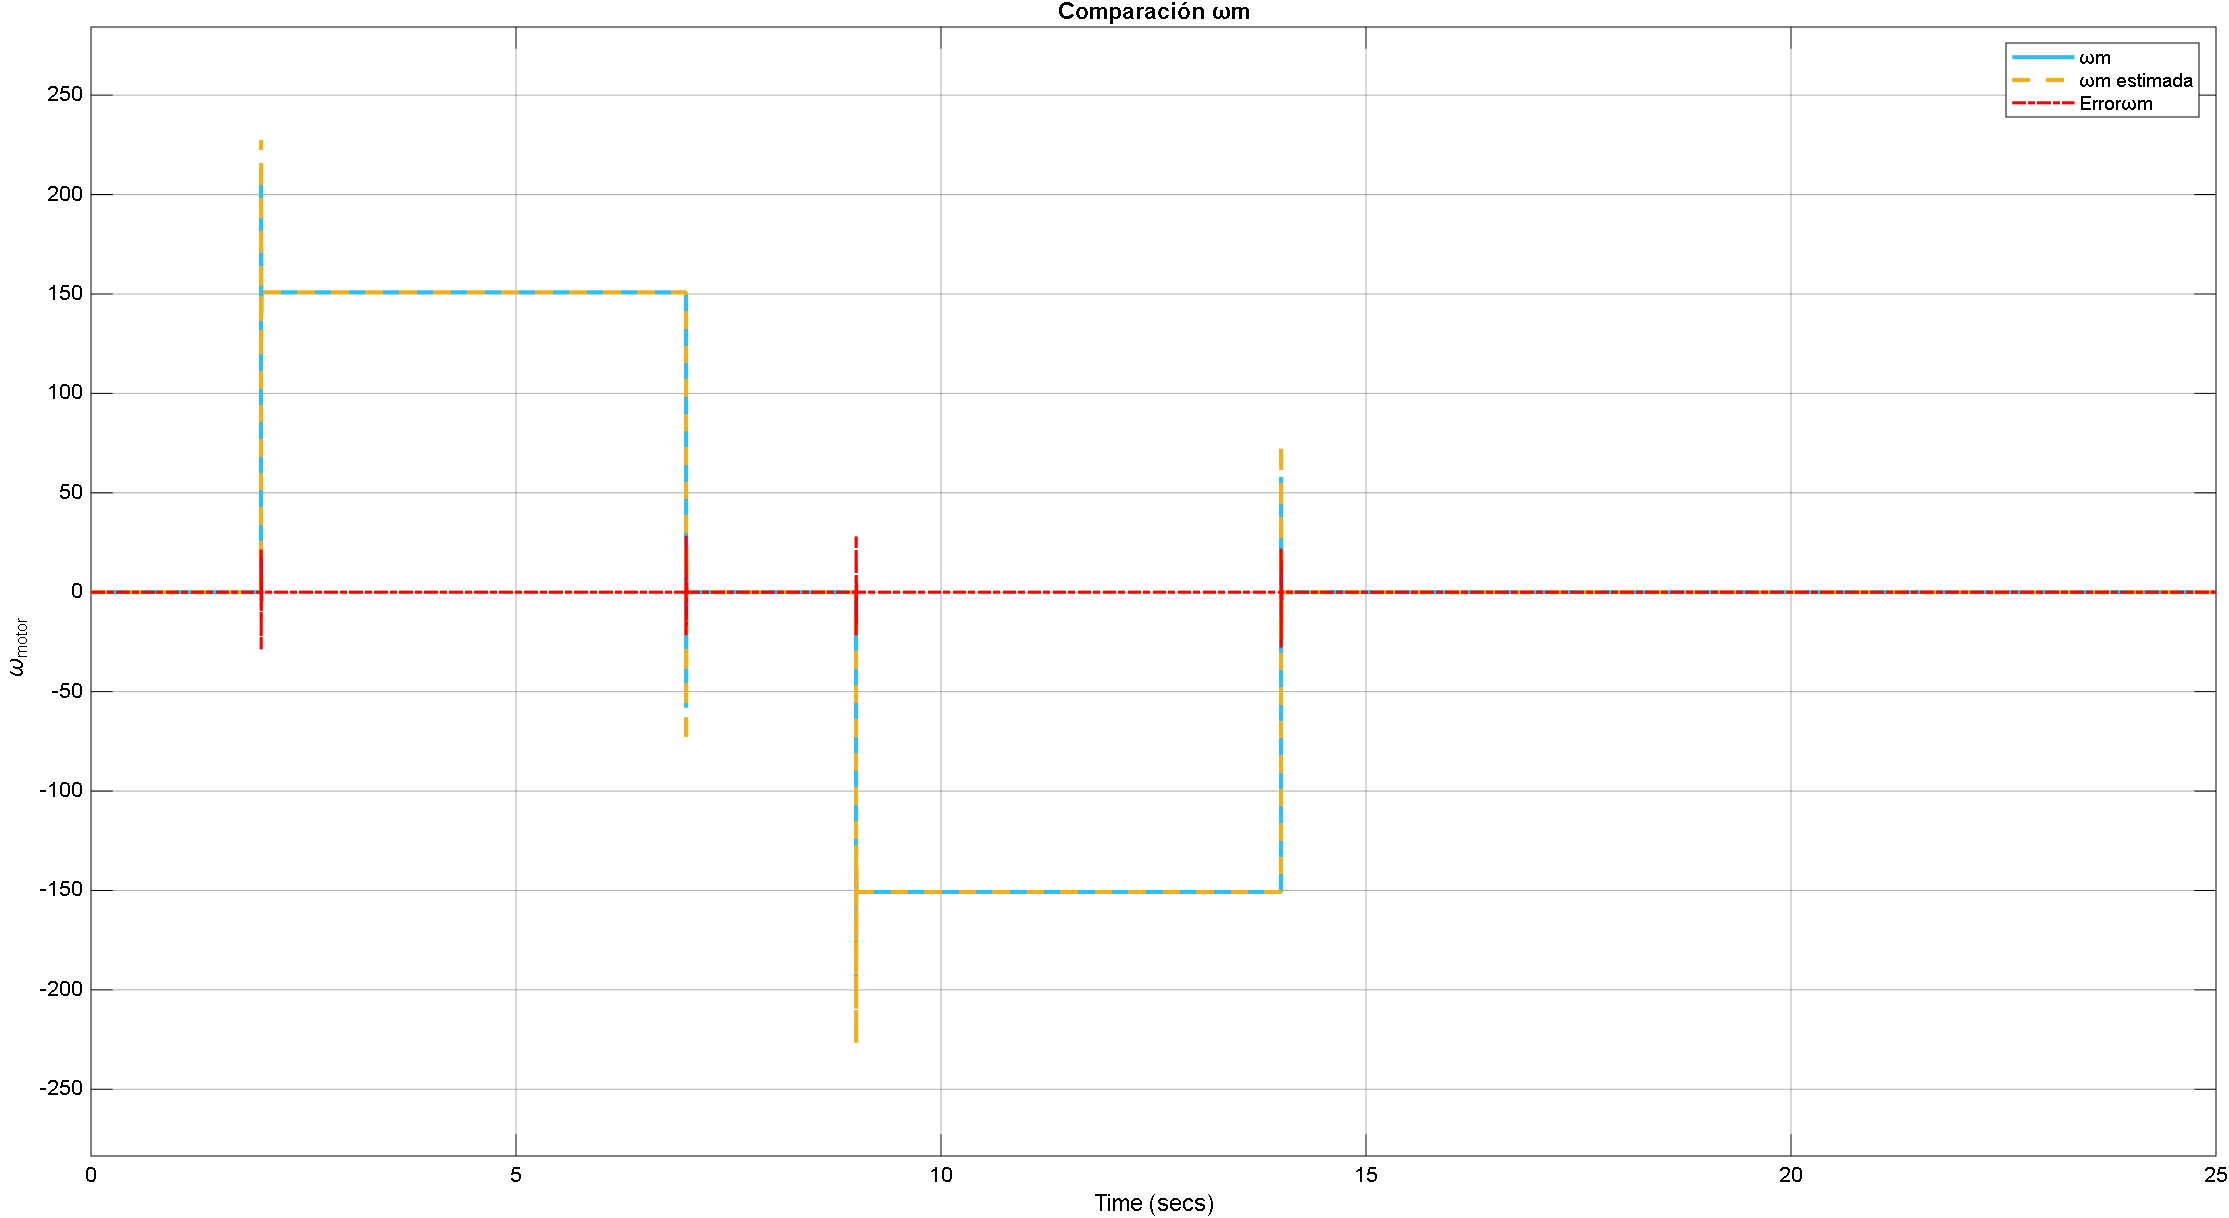
\includegraphics[trim=13.5bp 0 0 0,clip,width=0.86\linewidth,height=0.40\textheight,keepaspectratio]{attachments/comparacion estimacion velocidad angulan.png}
    \caption{Velocidad angular del motor $\omega_m$ (rad/s) con y sin estimación.}
    \label{fig:comparacion estimación velocidad angular}
    \par\medskip
    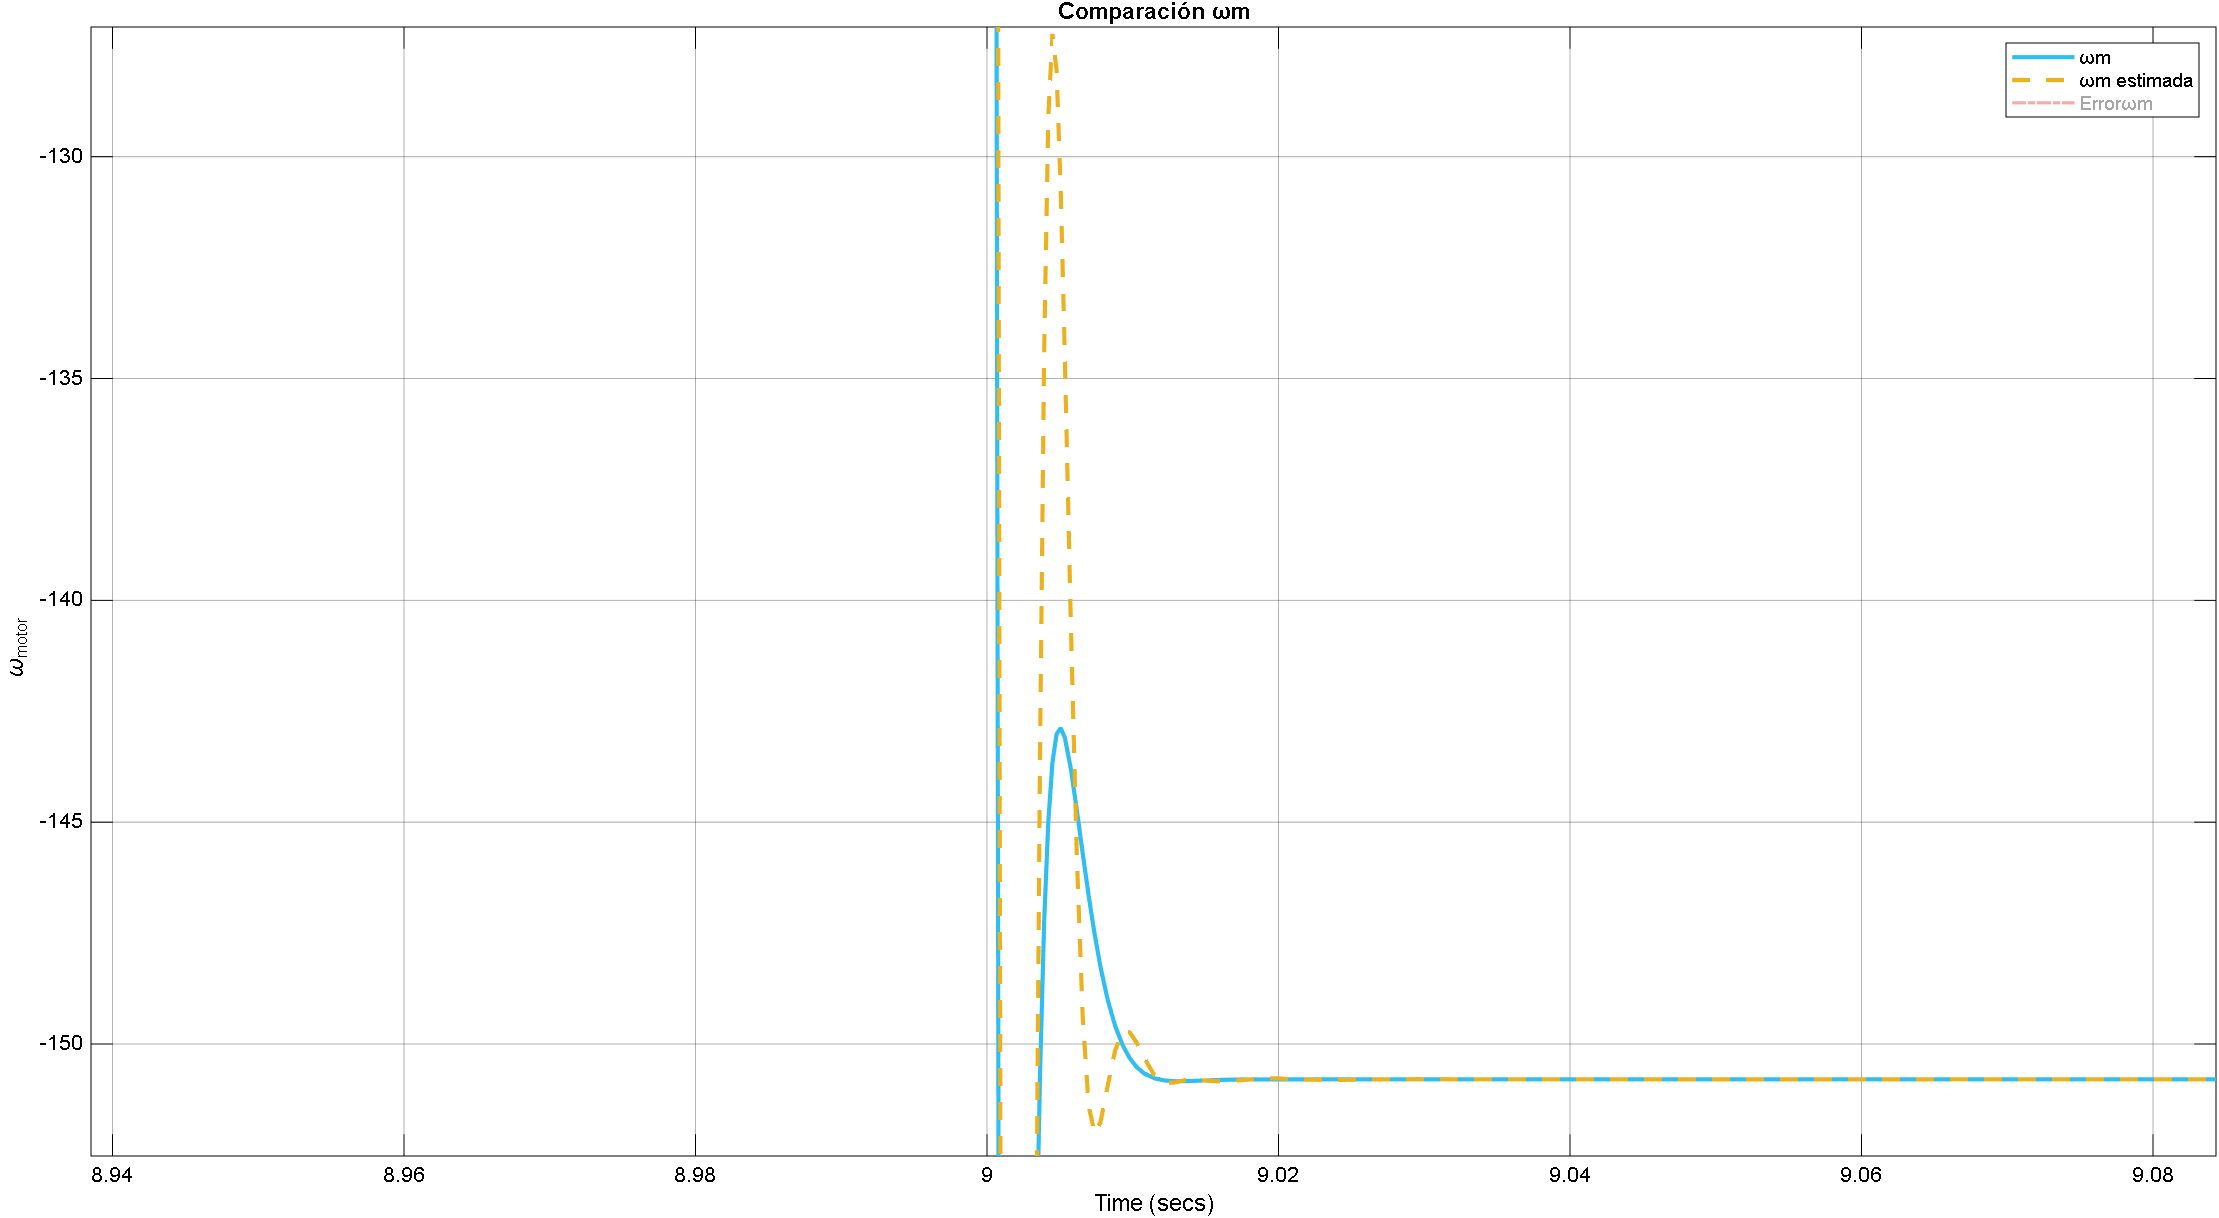
\includegraphics[trim=13.5bp 0 0 0,clip,width=0.86\linewidth,height=0.40\textheight,keepaspectratio]{attachments/DETALLE comparacion estimacion velocidad angulan.png}
    \caption{Detalle de la velocidad angular $\omega_m$ (rad/s) en la transición de $t=9\,\mathrm{s}$.}
    \label{fig:detalle comparacion estimación velocidad angular}
\end{figure}
\begin{figure}[!htbp]
    \centering
    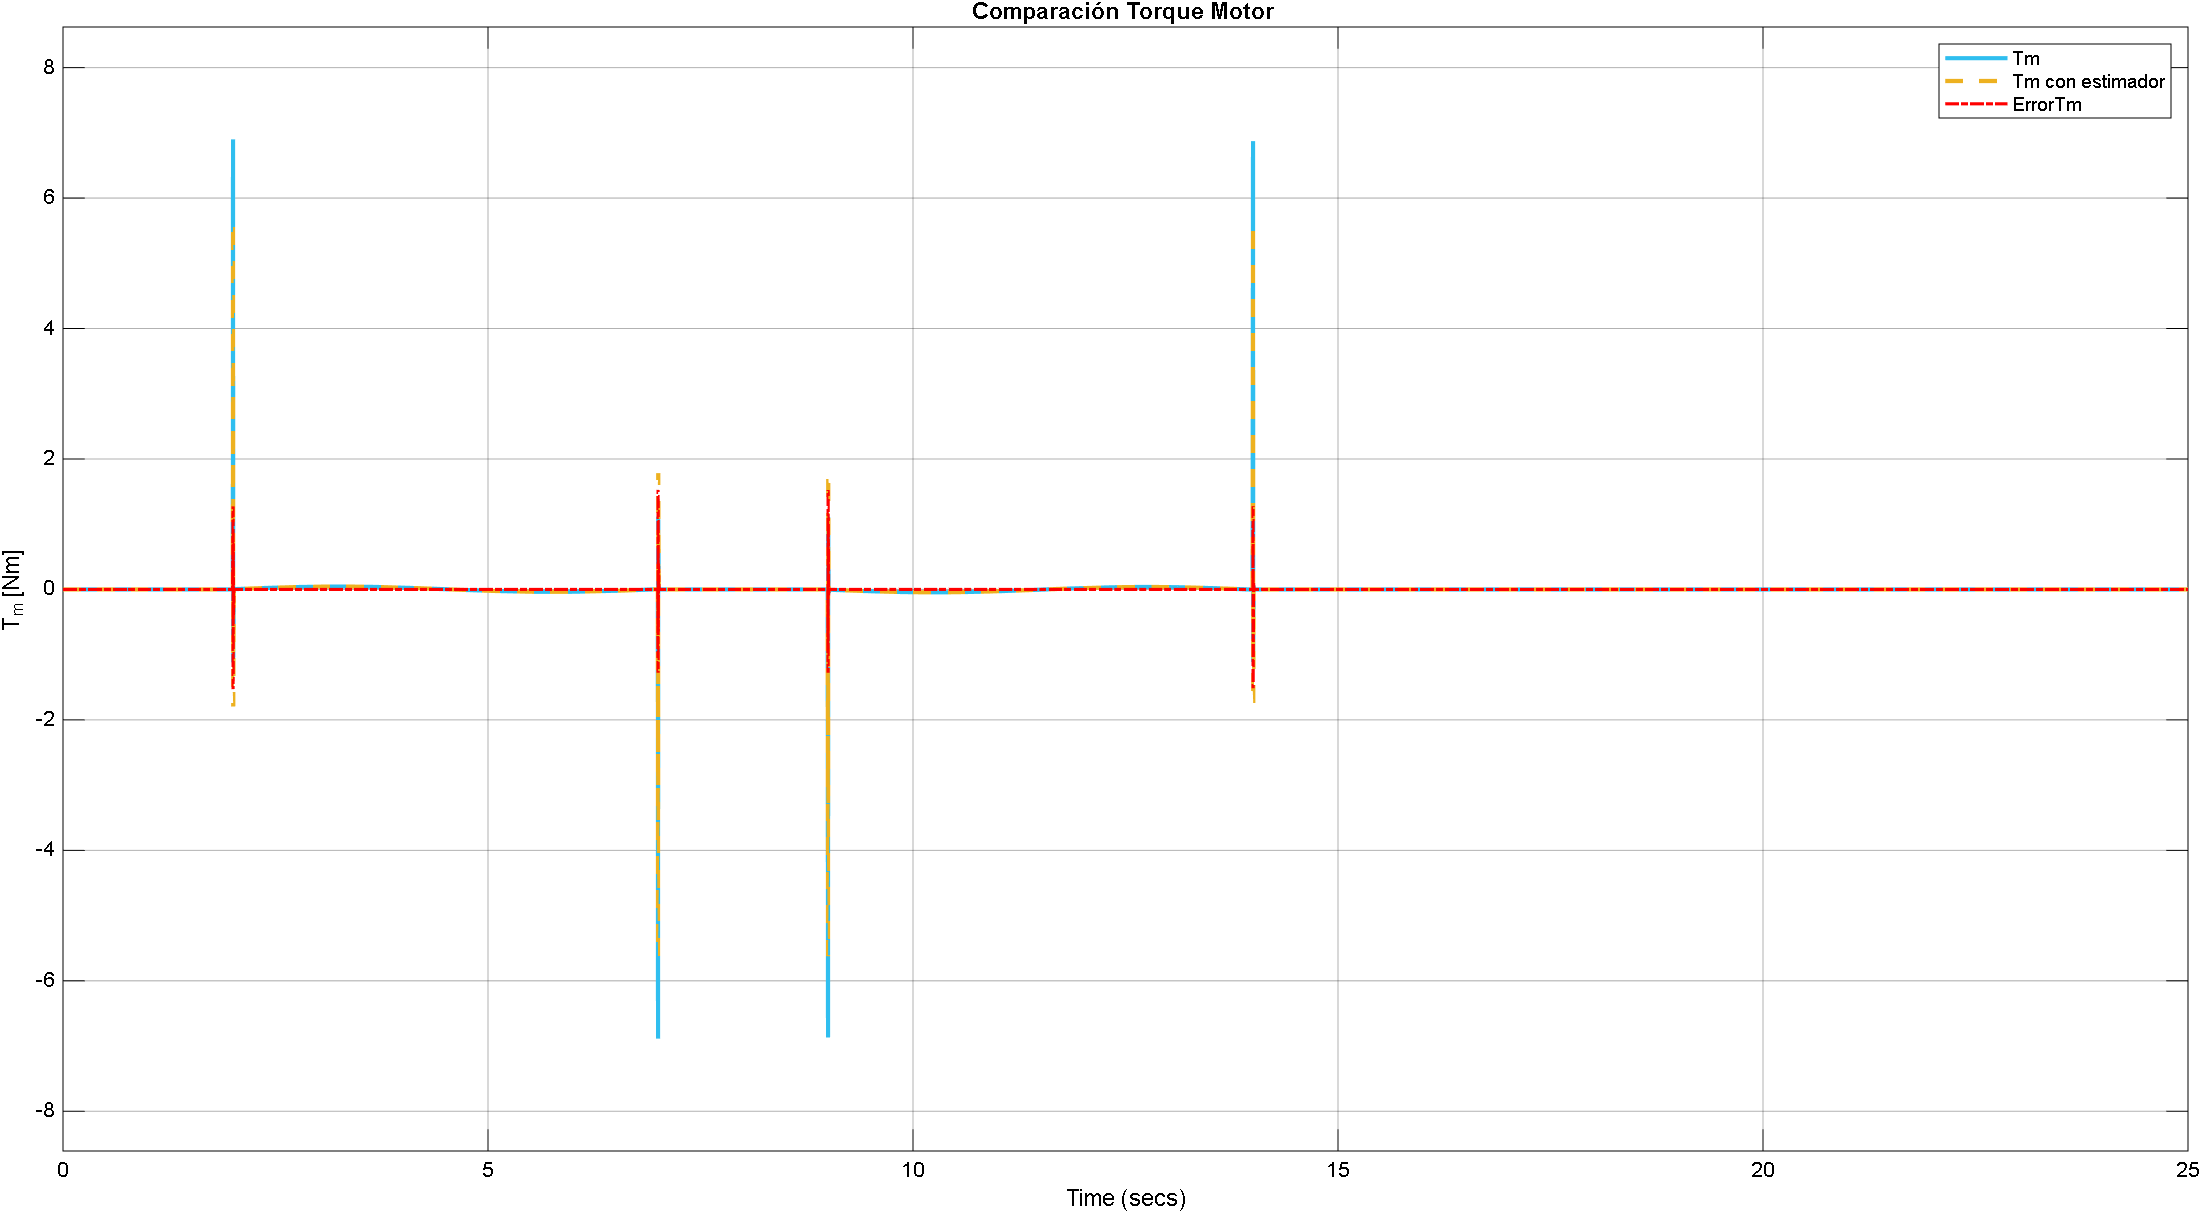
\includegraphics[width=0.86\linewidth,height=0.40\textheight,keepaspectratio]{attachments/comparacion estimacion torque motor.png}
    \caption{Comparación de $T_m$ entre los modelos con y sin estimación}
    \label{fig:comparacion estimación torque motor}
\end{figure}

\begin{figure}[!htbp]
    \centering
    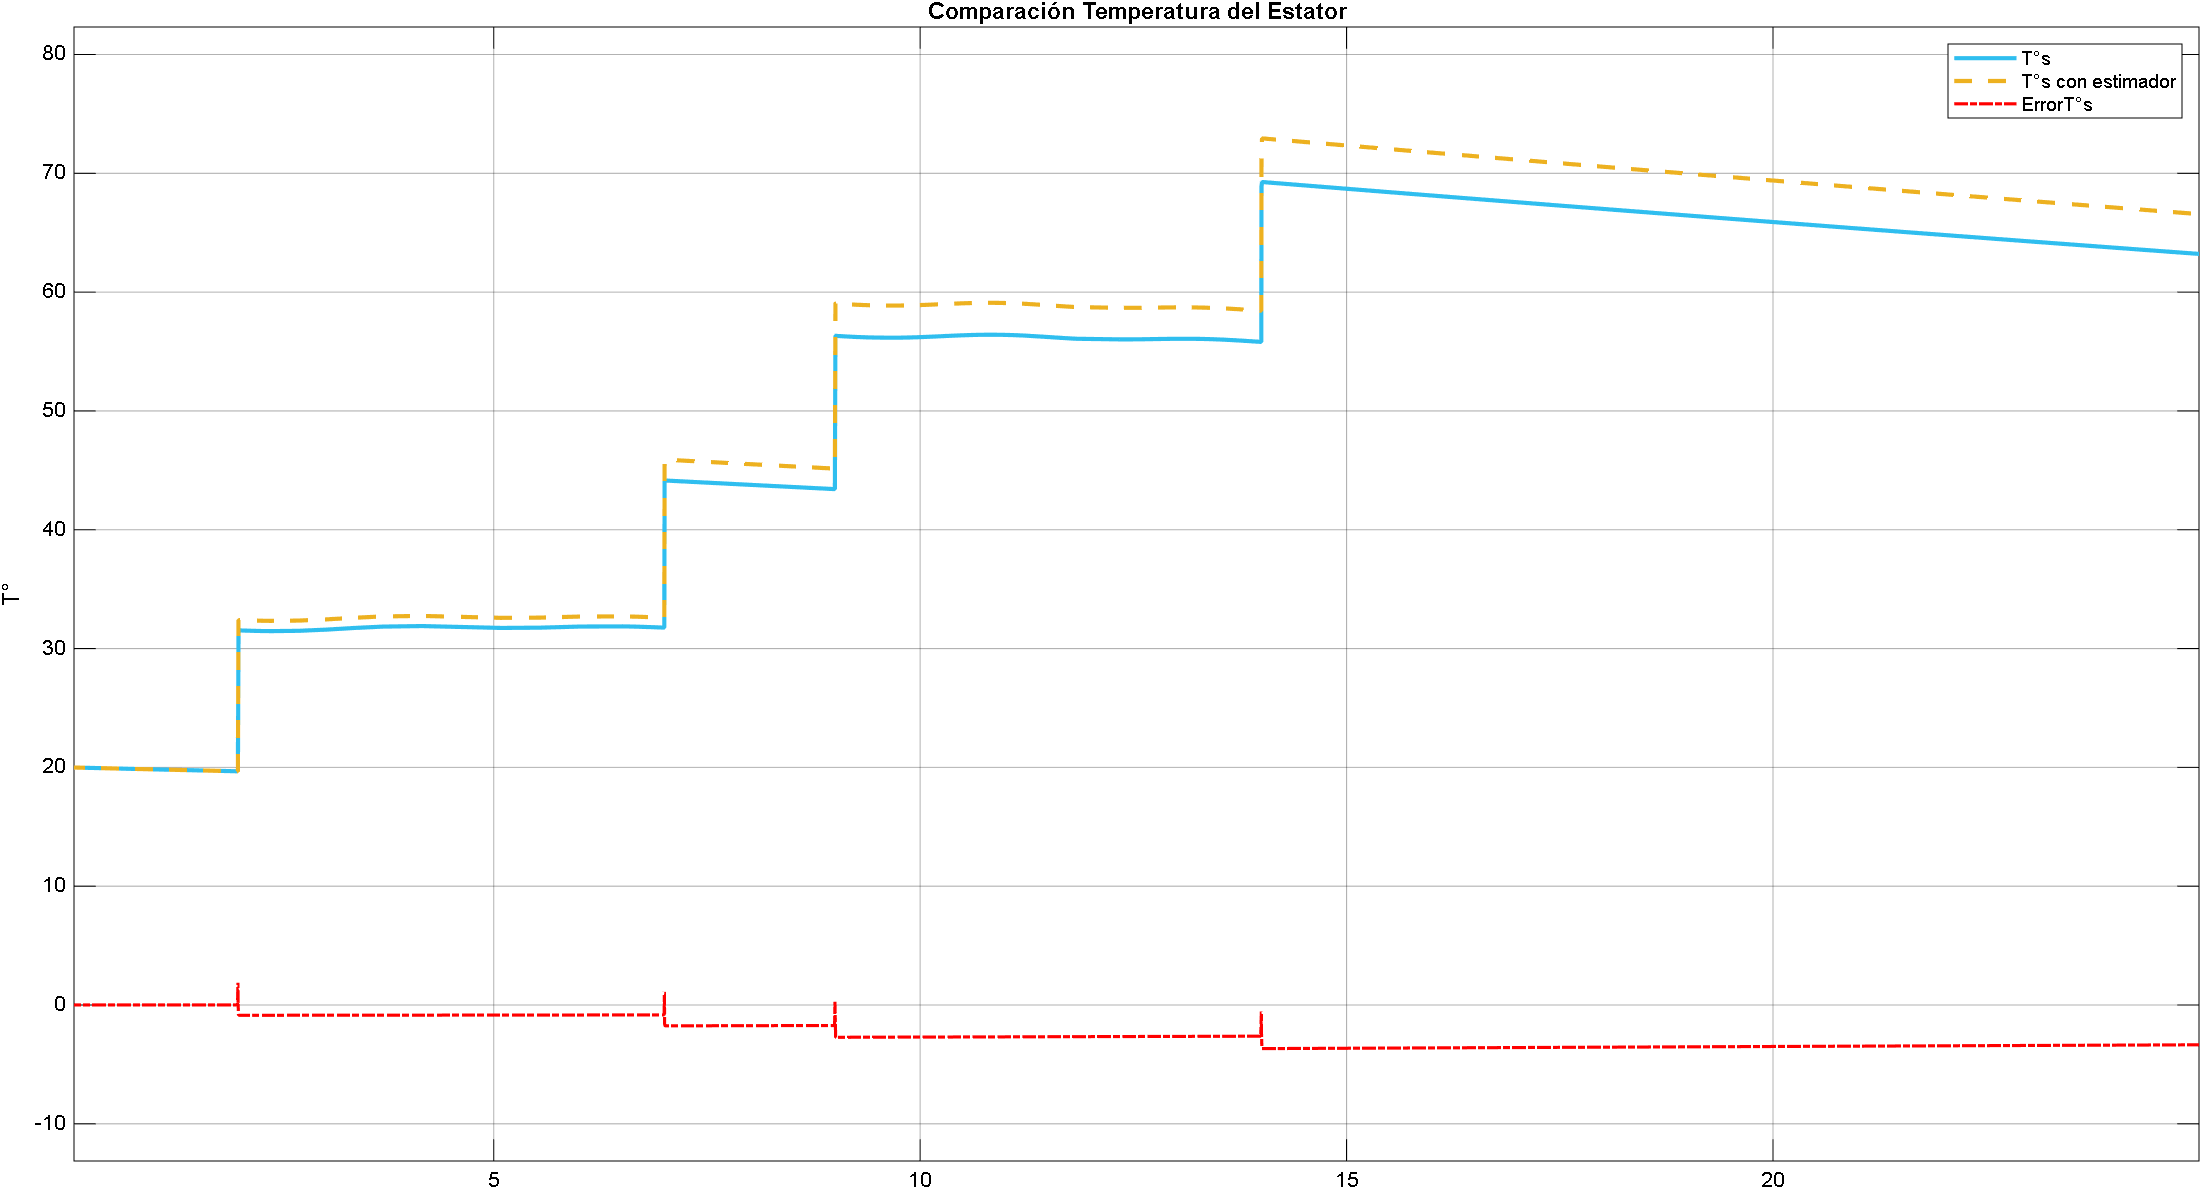
\includegraphics[width=0.86\linewidth,height=0.40\textheight,keepaspectratio]{attachments/comparacion estimacion temperatura del estator.png}
    \caption{Comparación de $T^\circ_s$ entre los modelos con y sin estimación}
    \label{fig:comparacion estimación temp estator}
\end{figure}
\begin{figure}[!htbp]
    \centering
    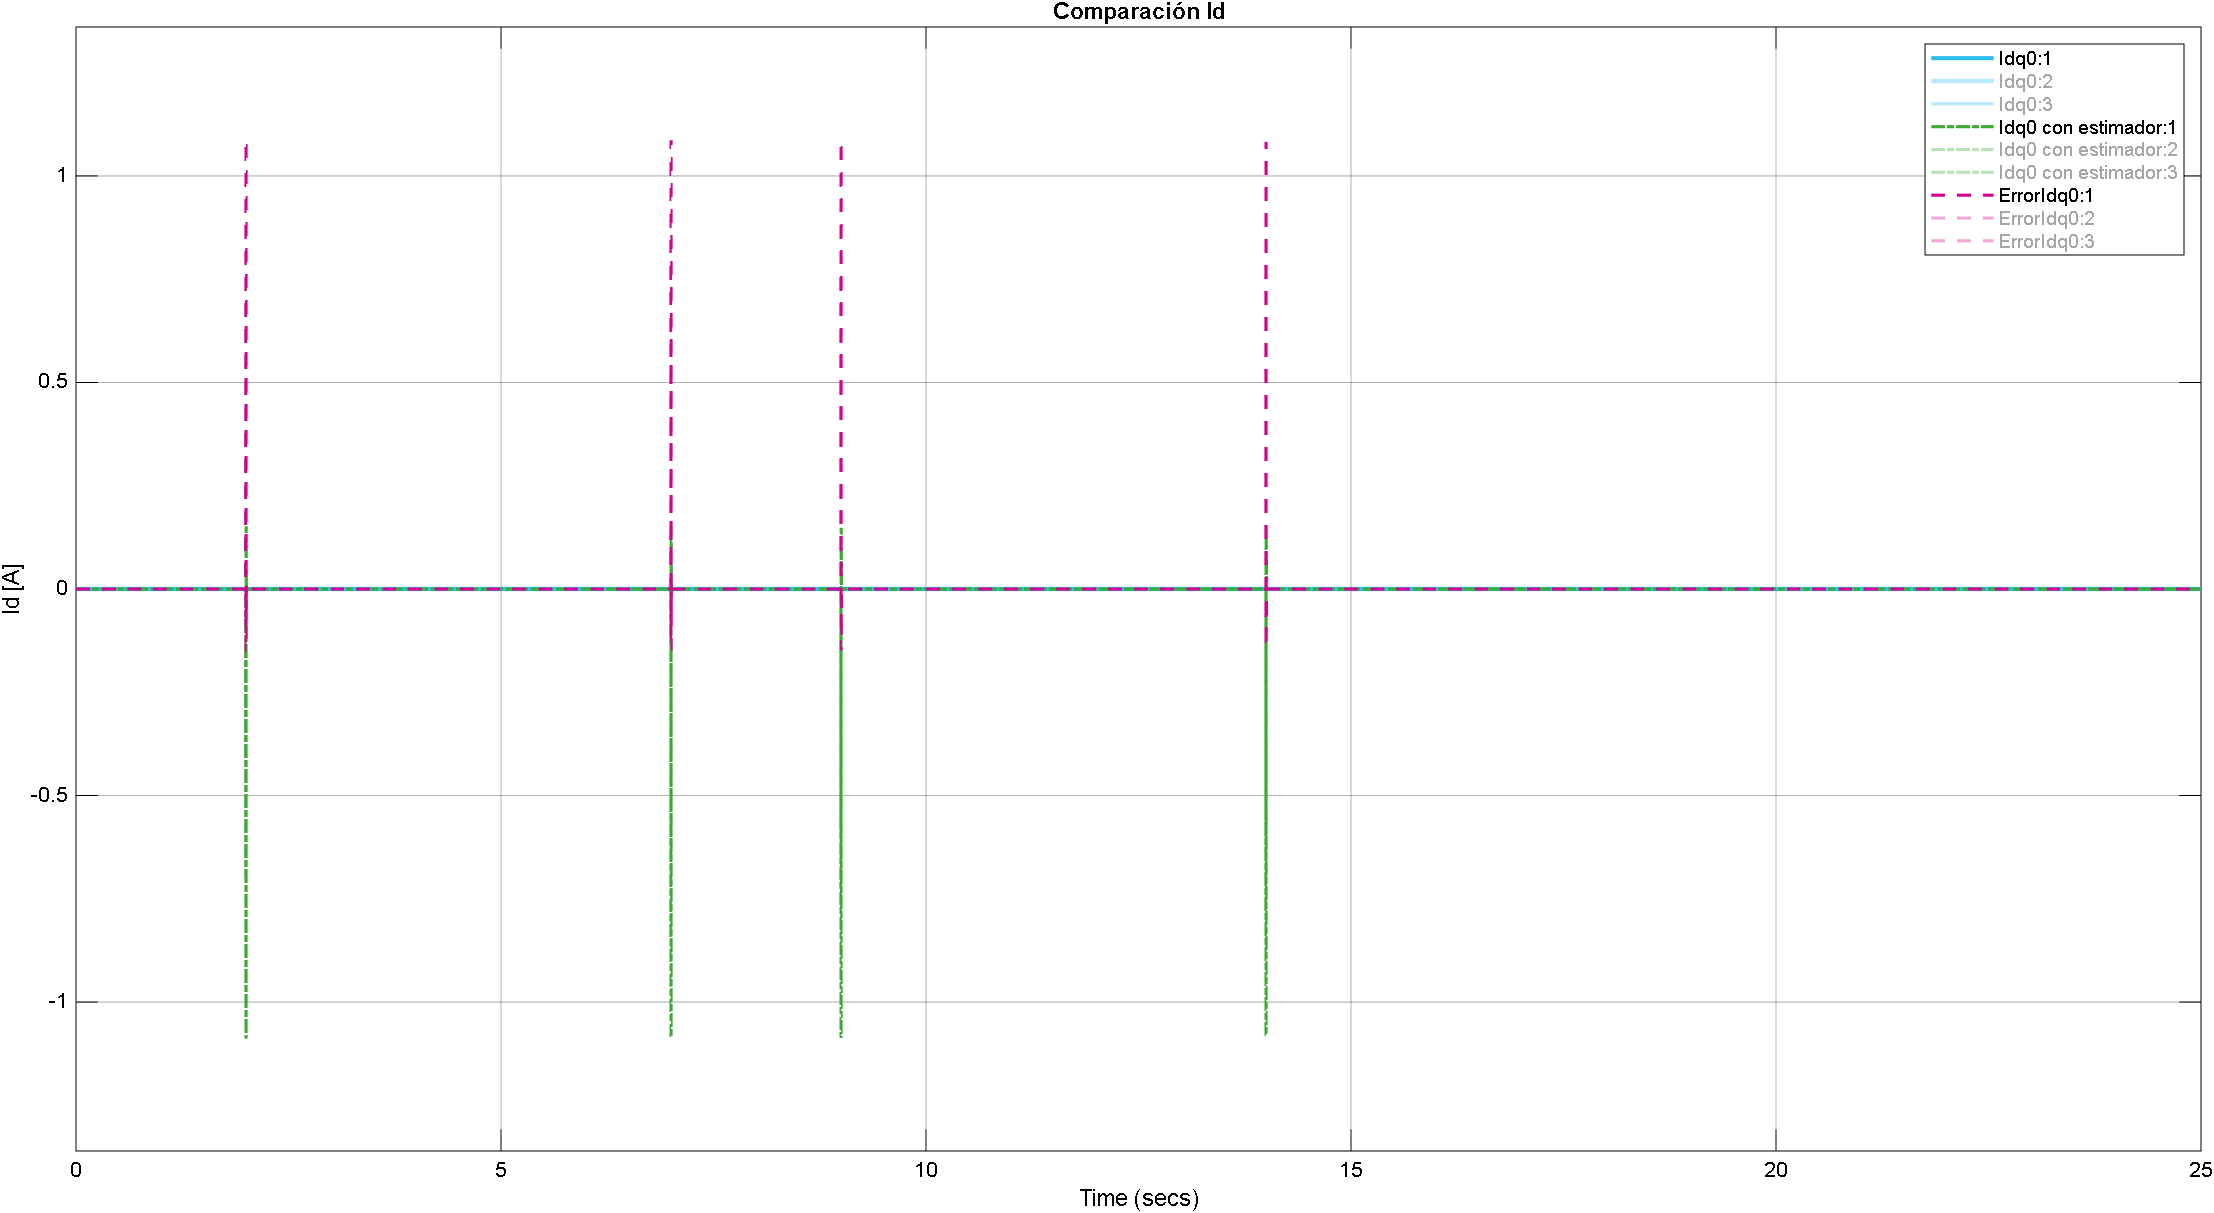
\includegraphics[width=0.86\linewidth,height=0.40\textheight,keepaspectratio]{attachments/comparacion estimacion corriente Id.png}
    \caption{Comparación de $i^r_{ds}$ entre los modelos con y sin estimación}
    \label{fig:comparacion estimación id}
\end{figure}
\begin{figure}[!htbp]
    \centering
    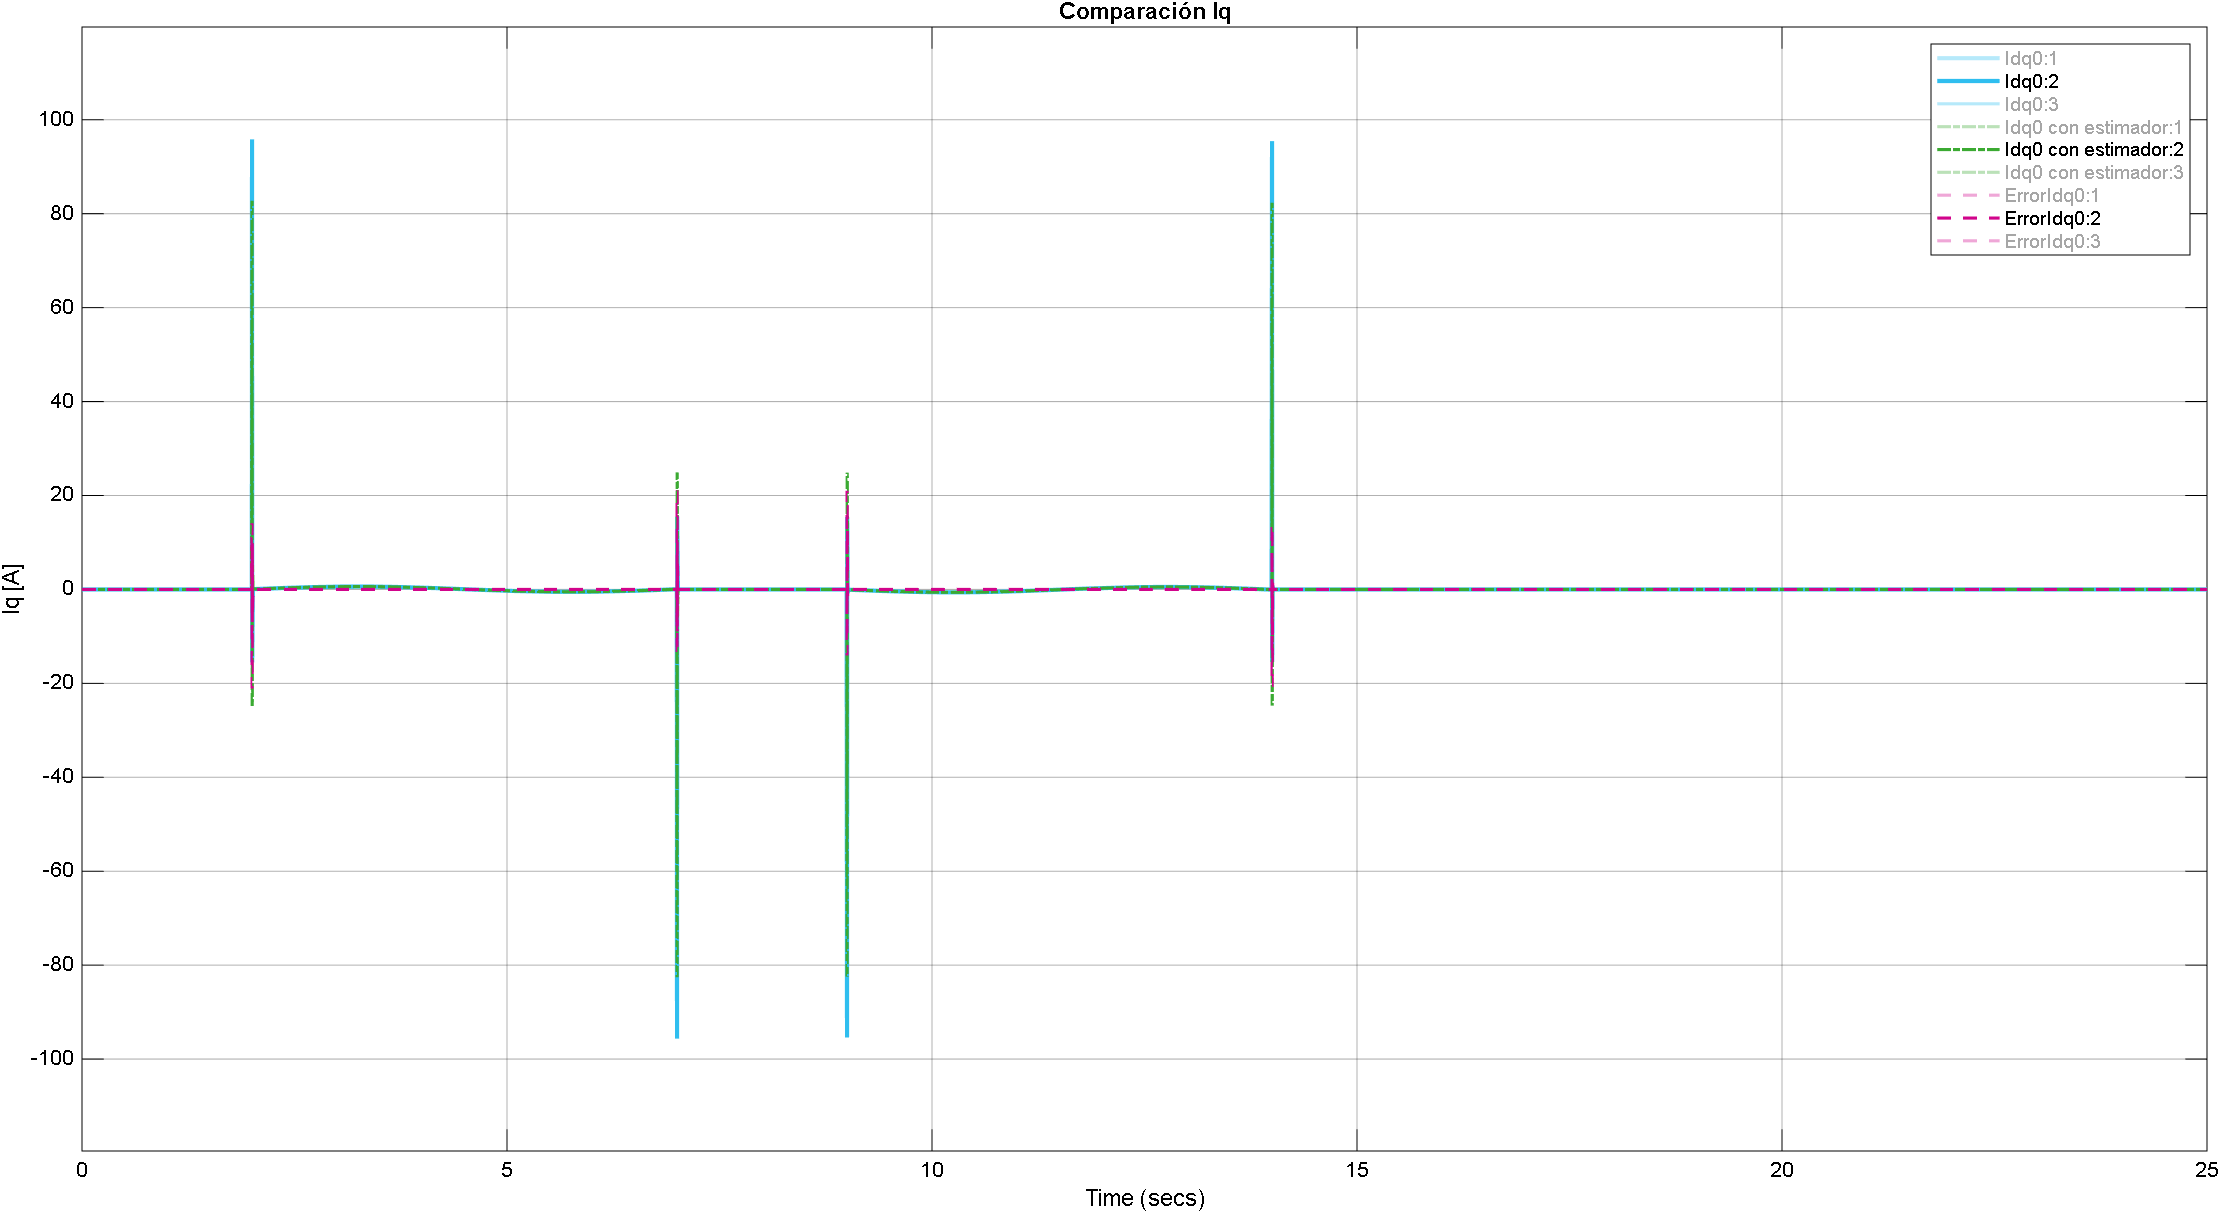
\includegraphics[width=0.86\linewidth,height=0.40\textheight,keepaspectratio]{attachments/comparacion estimacion corriente Iq.png}
    \caption{Comparación de $i^r_{qs}$ entre los modelos con y sin estimación}
    \label{fig:comparacion estimación iq}
\end{figure}
\begin{figure}[!htbp]
    \centering
    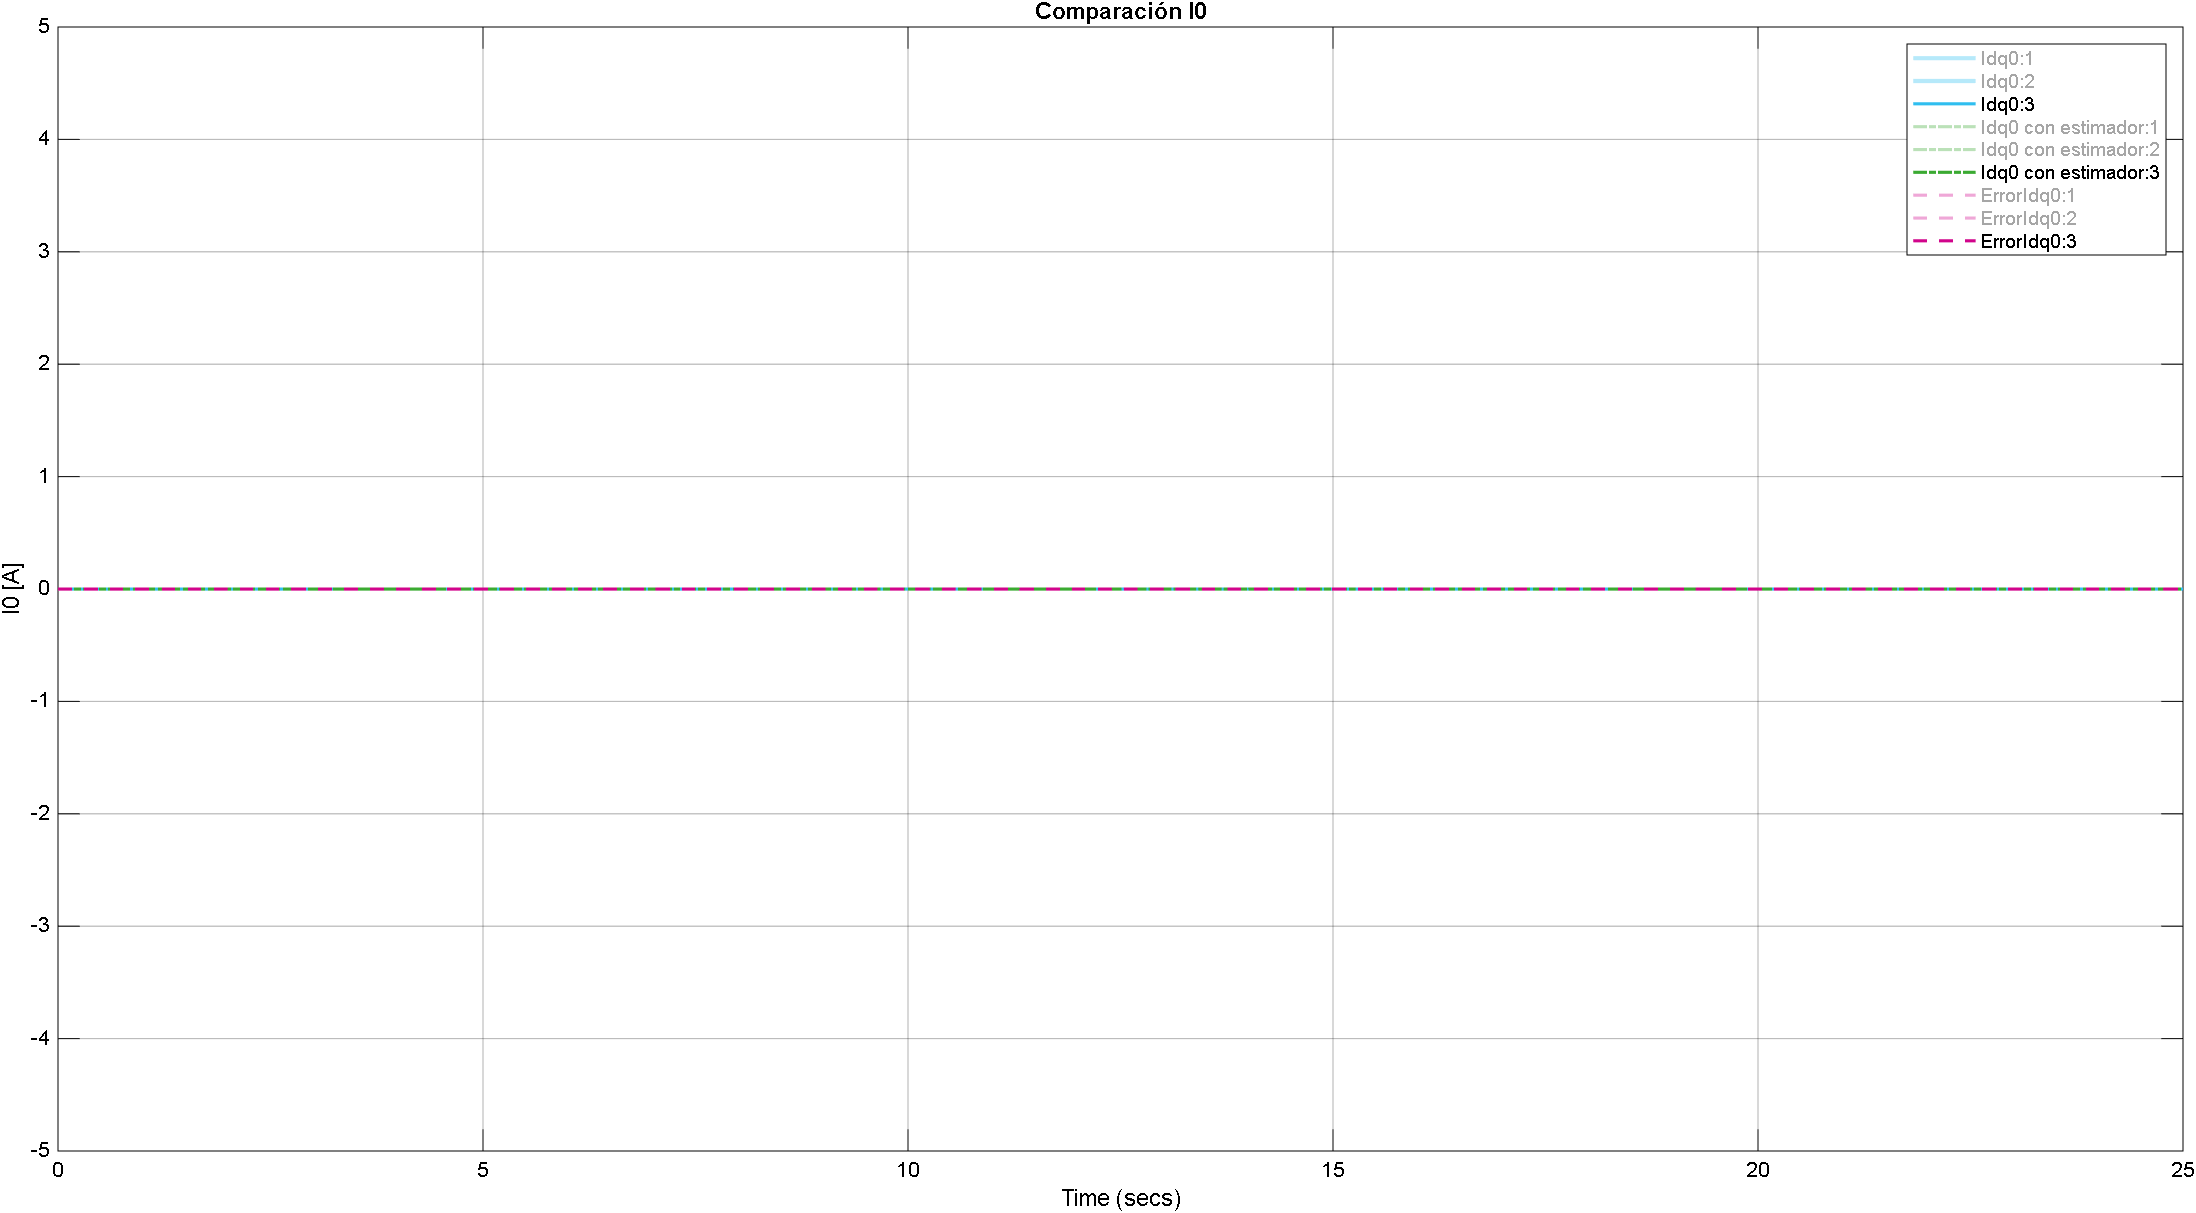
\includegraphics[width=0.86\linewidth,height=0.40\textheight,keepaspectratio]{attachments/comparacion estimacion corriente I0.png}
    \caption{Comparación de $i^r_{0s}$ entre los modelos con y sin estimación}
    \label{fig:comparacion estimación i0}
\end{figure}
Es posible ver que $\theta_m$ se comporta de forma trapezoidal al igual que la consigna de movimiento que se le ha dado en el eje multiplicado por la relación de reducción, se ve también que con los cambios repentinos de derivada de la consigna de movimiento se generan picos o cambios bruscos en $\omega_m$, $T_m$, $i_{ds}^r$ y $i_{qs}^r$. Estos picos especialmente en las corrientes y el torque generan problemas en una implementación real por lo que sería ideal que la consigna sea más suave para prevenir los picos.
\subsubsection{Rechazo a perturbaciones}
\label{subsubsec: rechazo a perturbaciones}
Al modelo se le plantea una perturbación de torque en forma de escalón y luego se analiza el comportamiento del modelo. El análisis
se hará teniendo en cuenta una masa de carga $m_l = 0,5\;$kg, una temperatura ambiente $T_{amb} = 20^\circ C$, con consignas de velocidad angular $\omega_m$ y posición angular $\theta_m$ nulos, y una perturbacíon de carga $T_{ld}=+5Nm$ de tipo escalón.

\begin{figure}[!htbp]
    \centering
    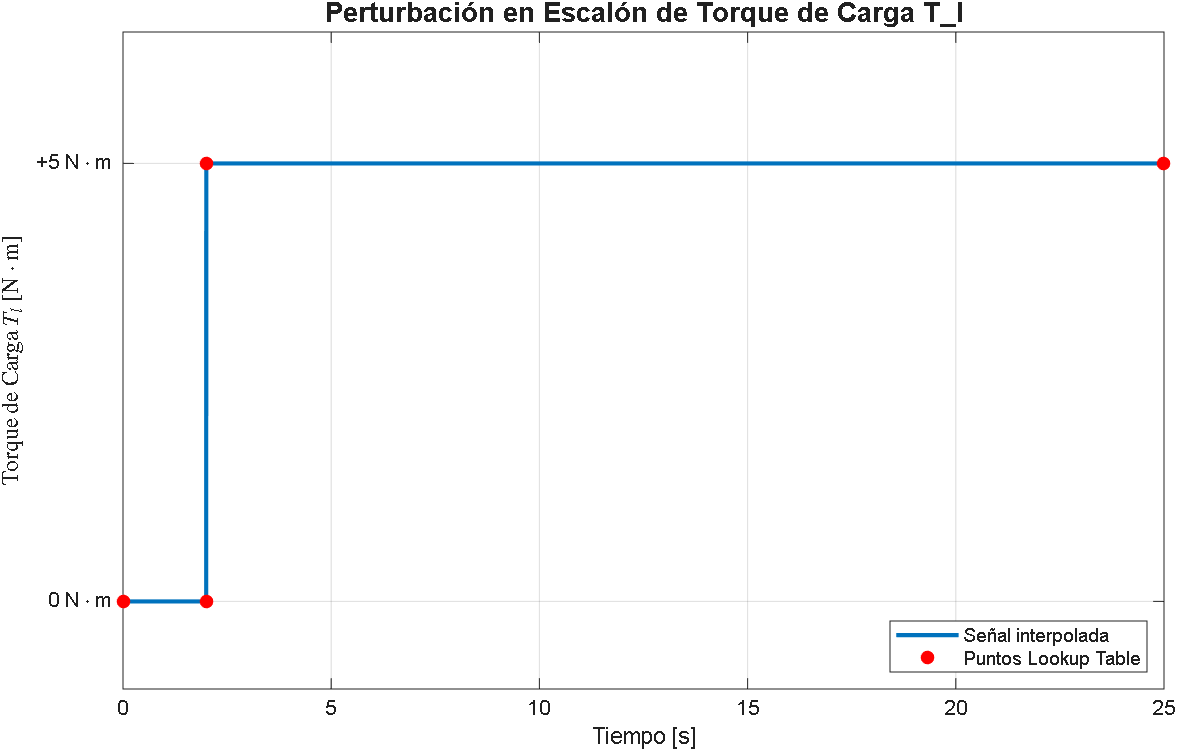
\includegraphics[width=0.76\linewidth,height=0.38\textheight,keepaspectratio]{attachments/Perturbacion escalon de torque.png}
    \caption{Perturbación escalón $T_{ld}$}
    \label{fig:perturbacion tl}
\end{figure}
\begin{figure}[!htbp]
    \centering
    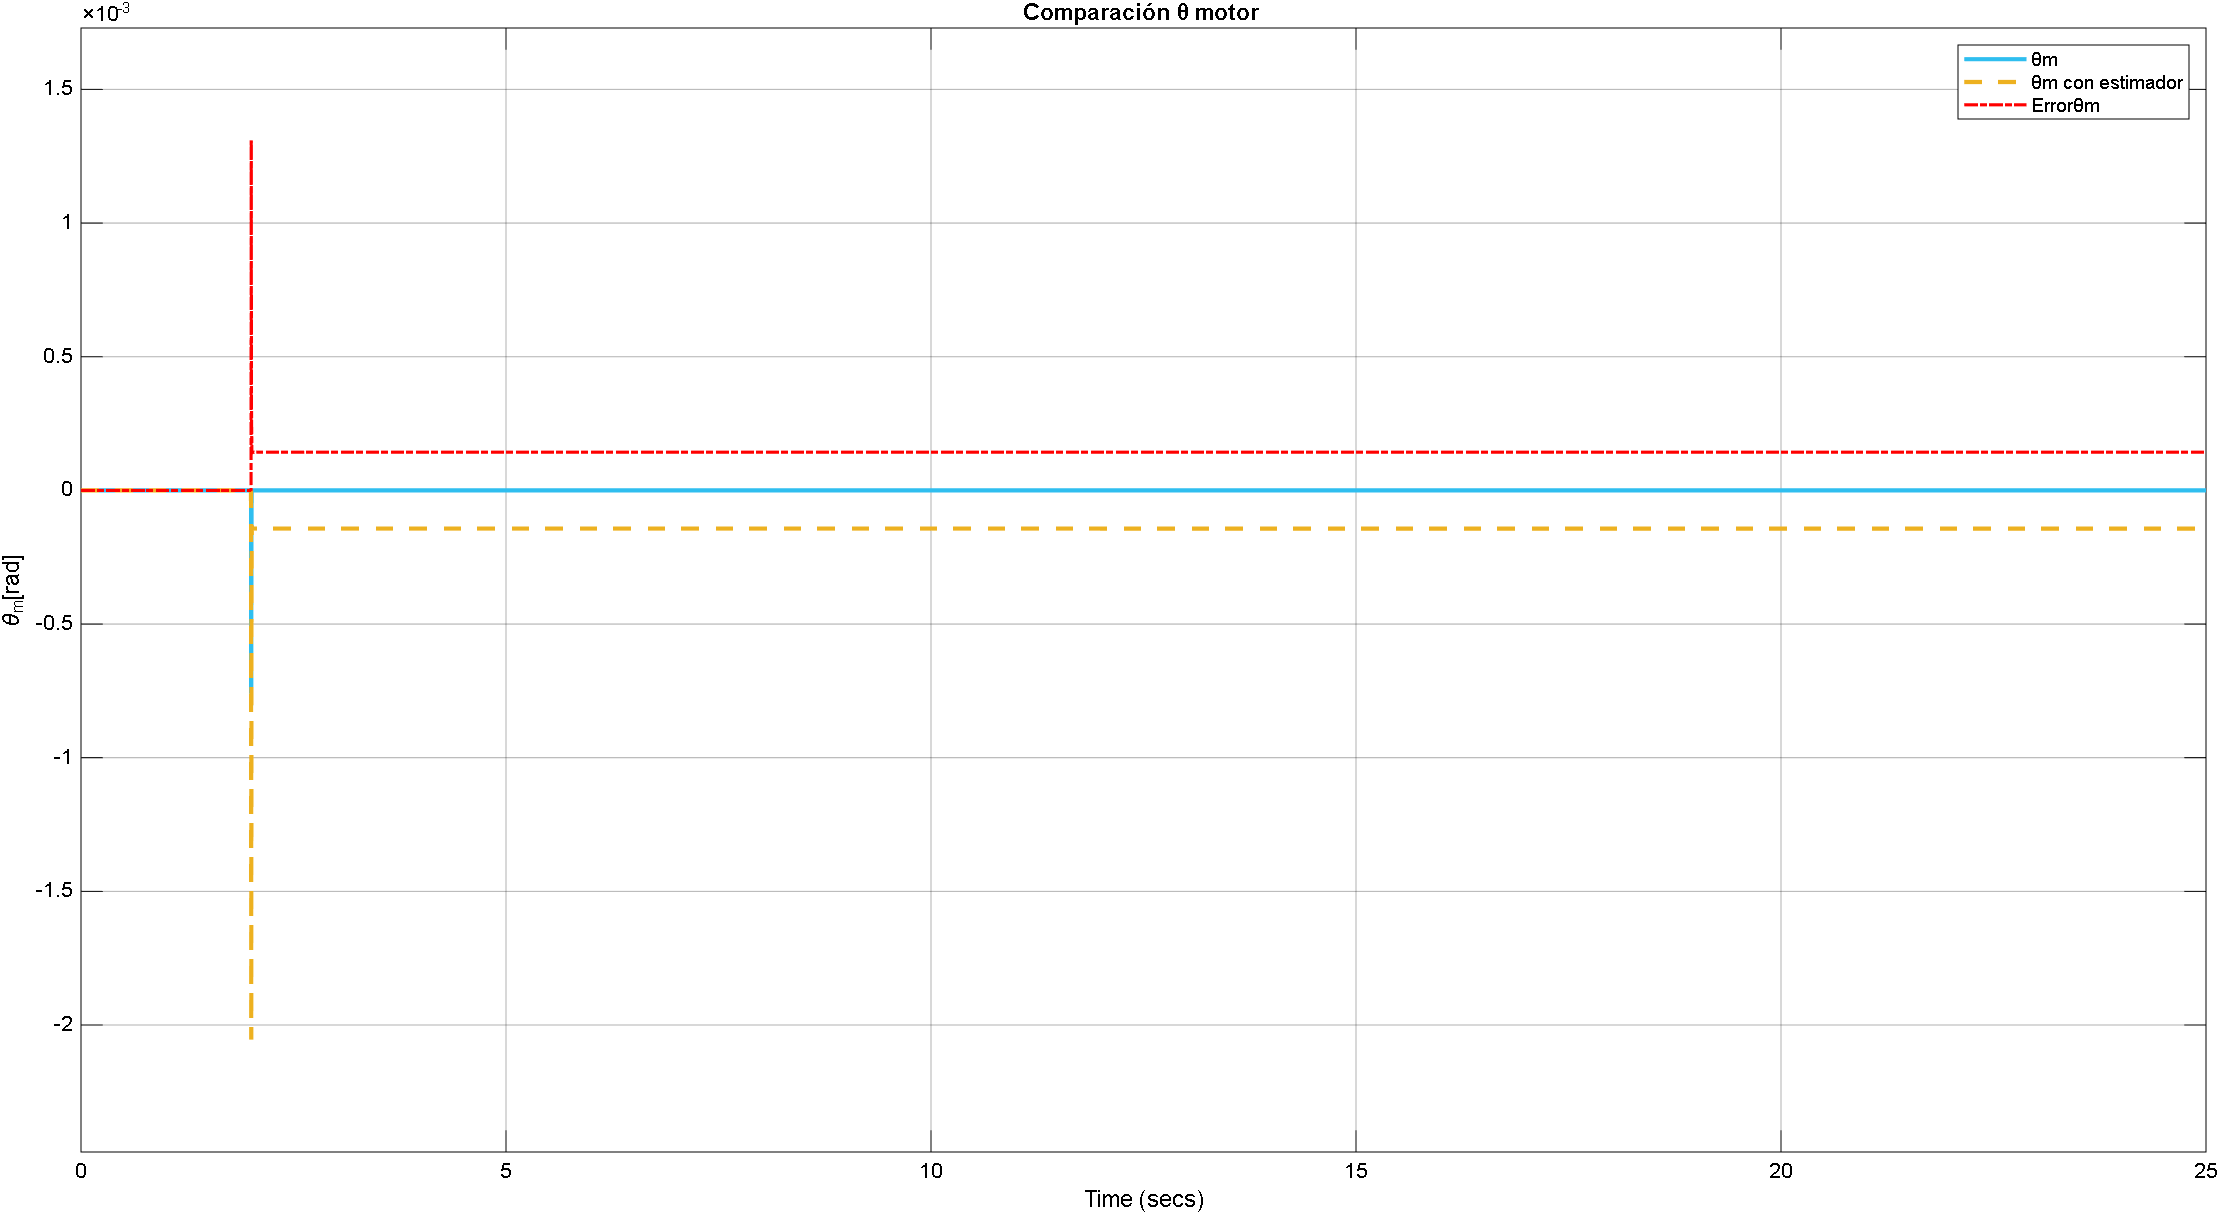
\includegraphics[width=0.86\linewidth,height=0.40\textheight,keepaspectratio]{attachments/comparacion estimacion posicion angulan con perturbacion.png}
    \caption{Comparación de $\theta_m$ entre los modelos con y sin estimación debido a la perturbación en torque $T_{ld}$}
    \label{fig:comparacion estimación posicion angular con perturbacion de torque}
\end{figure}
\begin{figure}[!htbp]
    \centering
    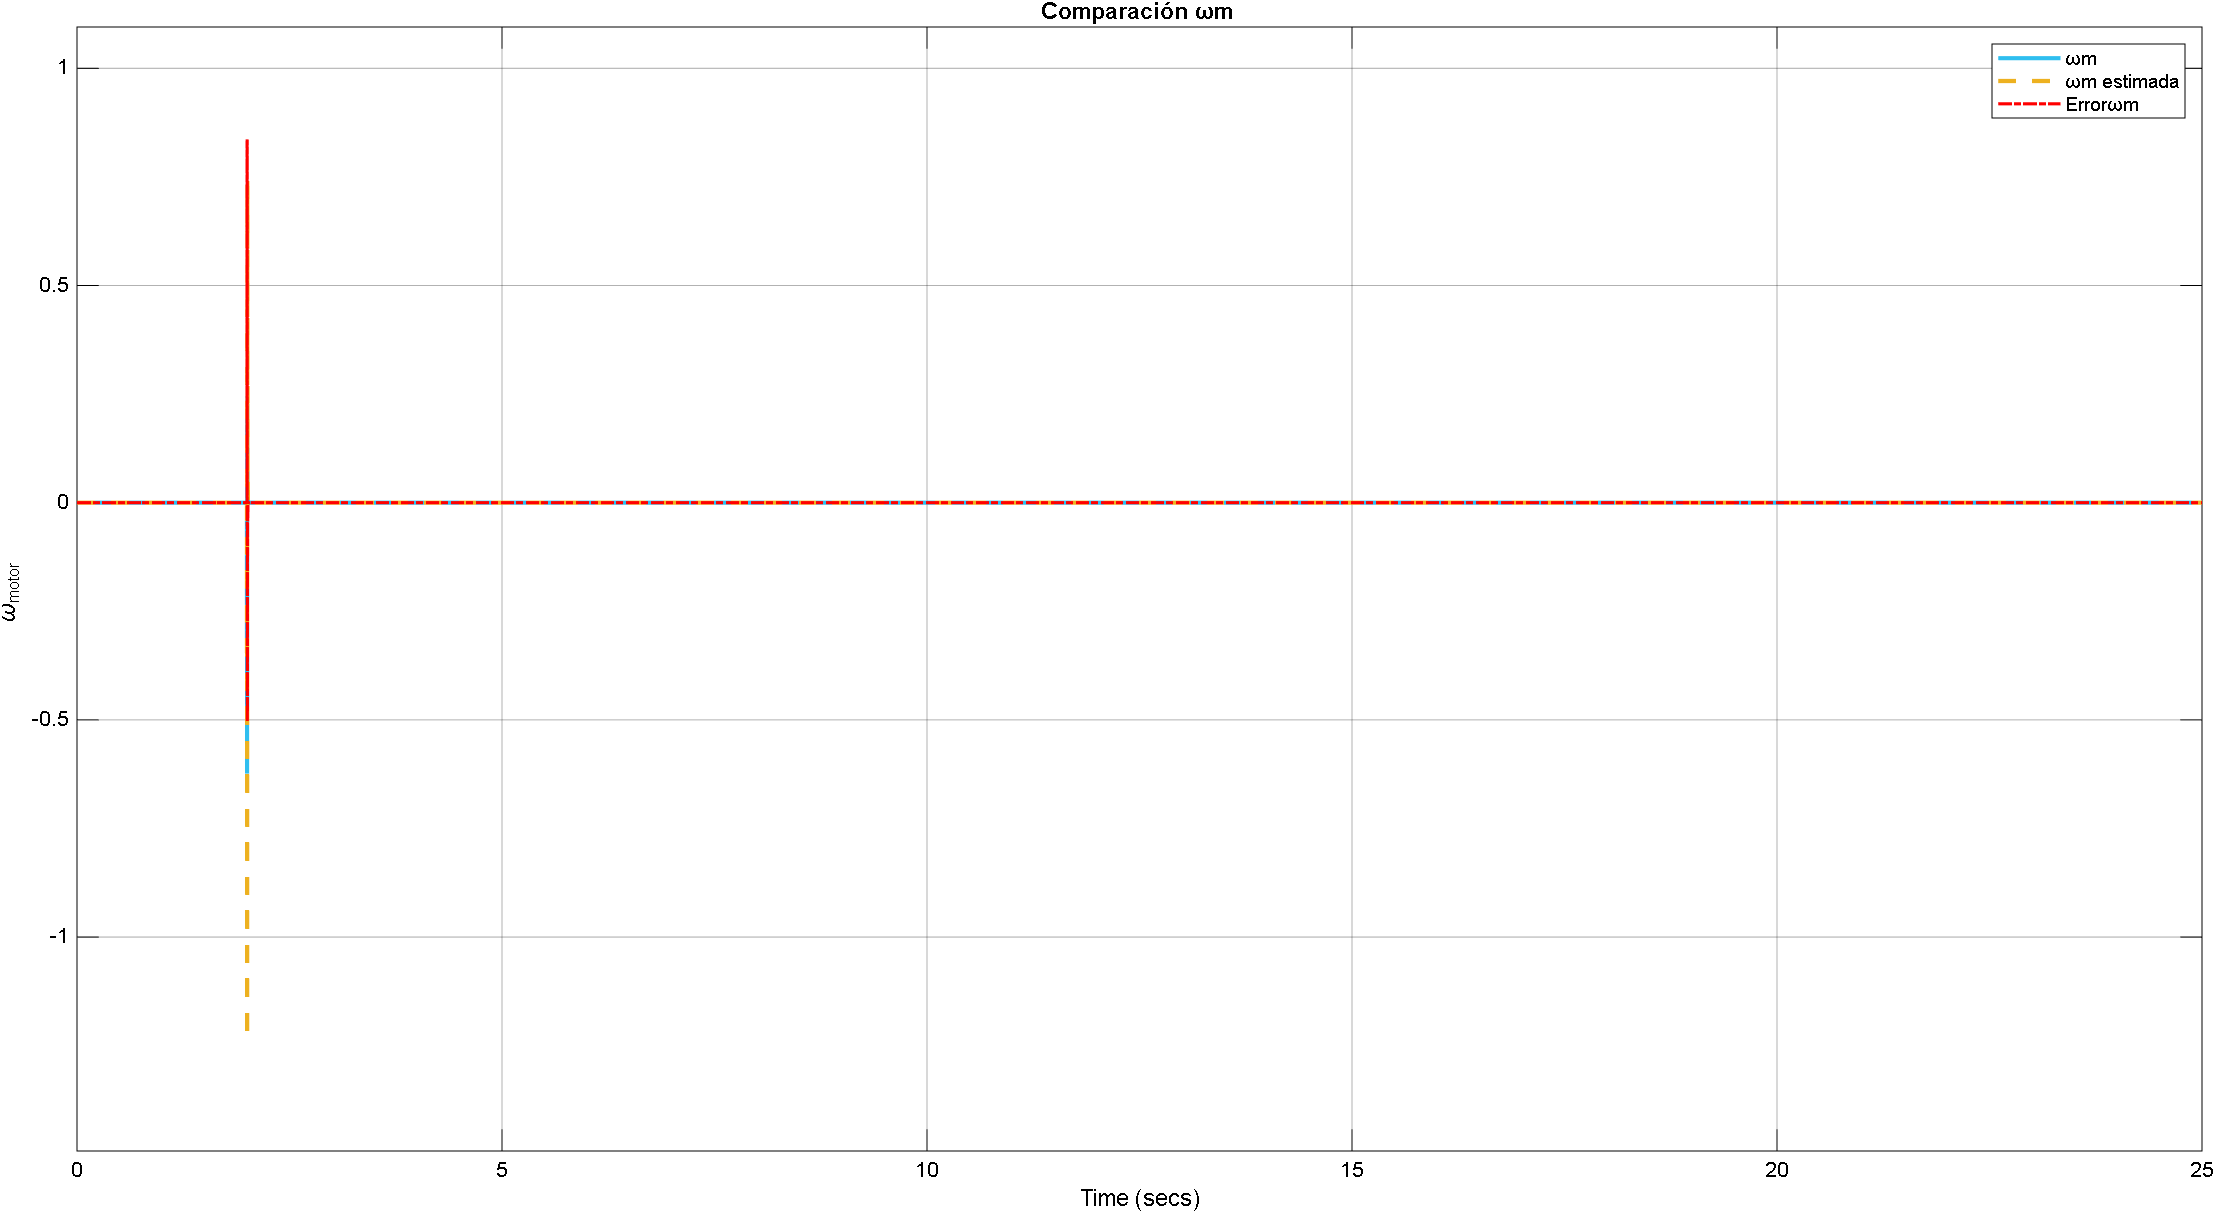
\includegraphics[width=0.86\linewidth,height=0.40\textheight,keepaspectratio]{attachments/comparacion estimacion velocidad angulan con perturbacion.png}
    \caption{Comparación de $\omega_m$ entre los modelos con y sin estimación debido a la perturbación en torque $T_{ld}$}
    \label{fig:comparacion estimación velocidad angular con perturbacion de torque}
    \par\medskip
    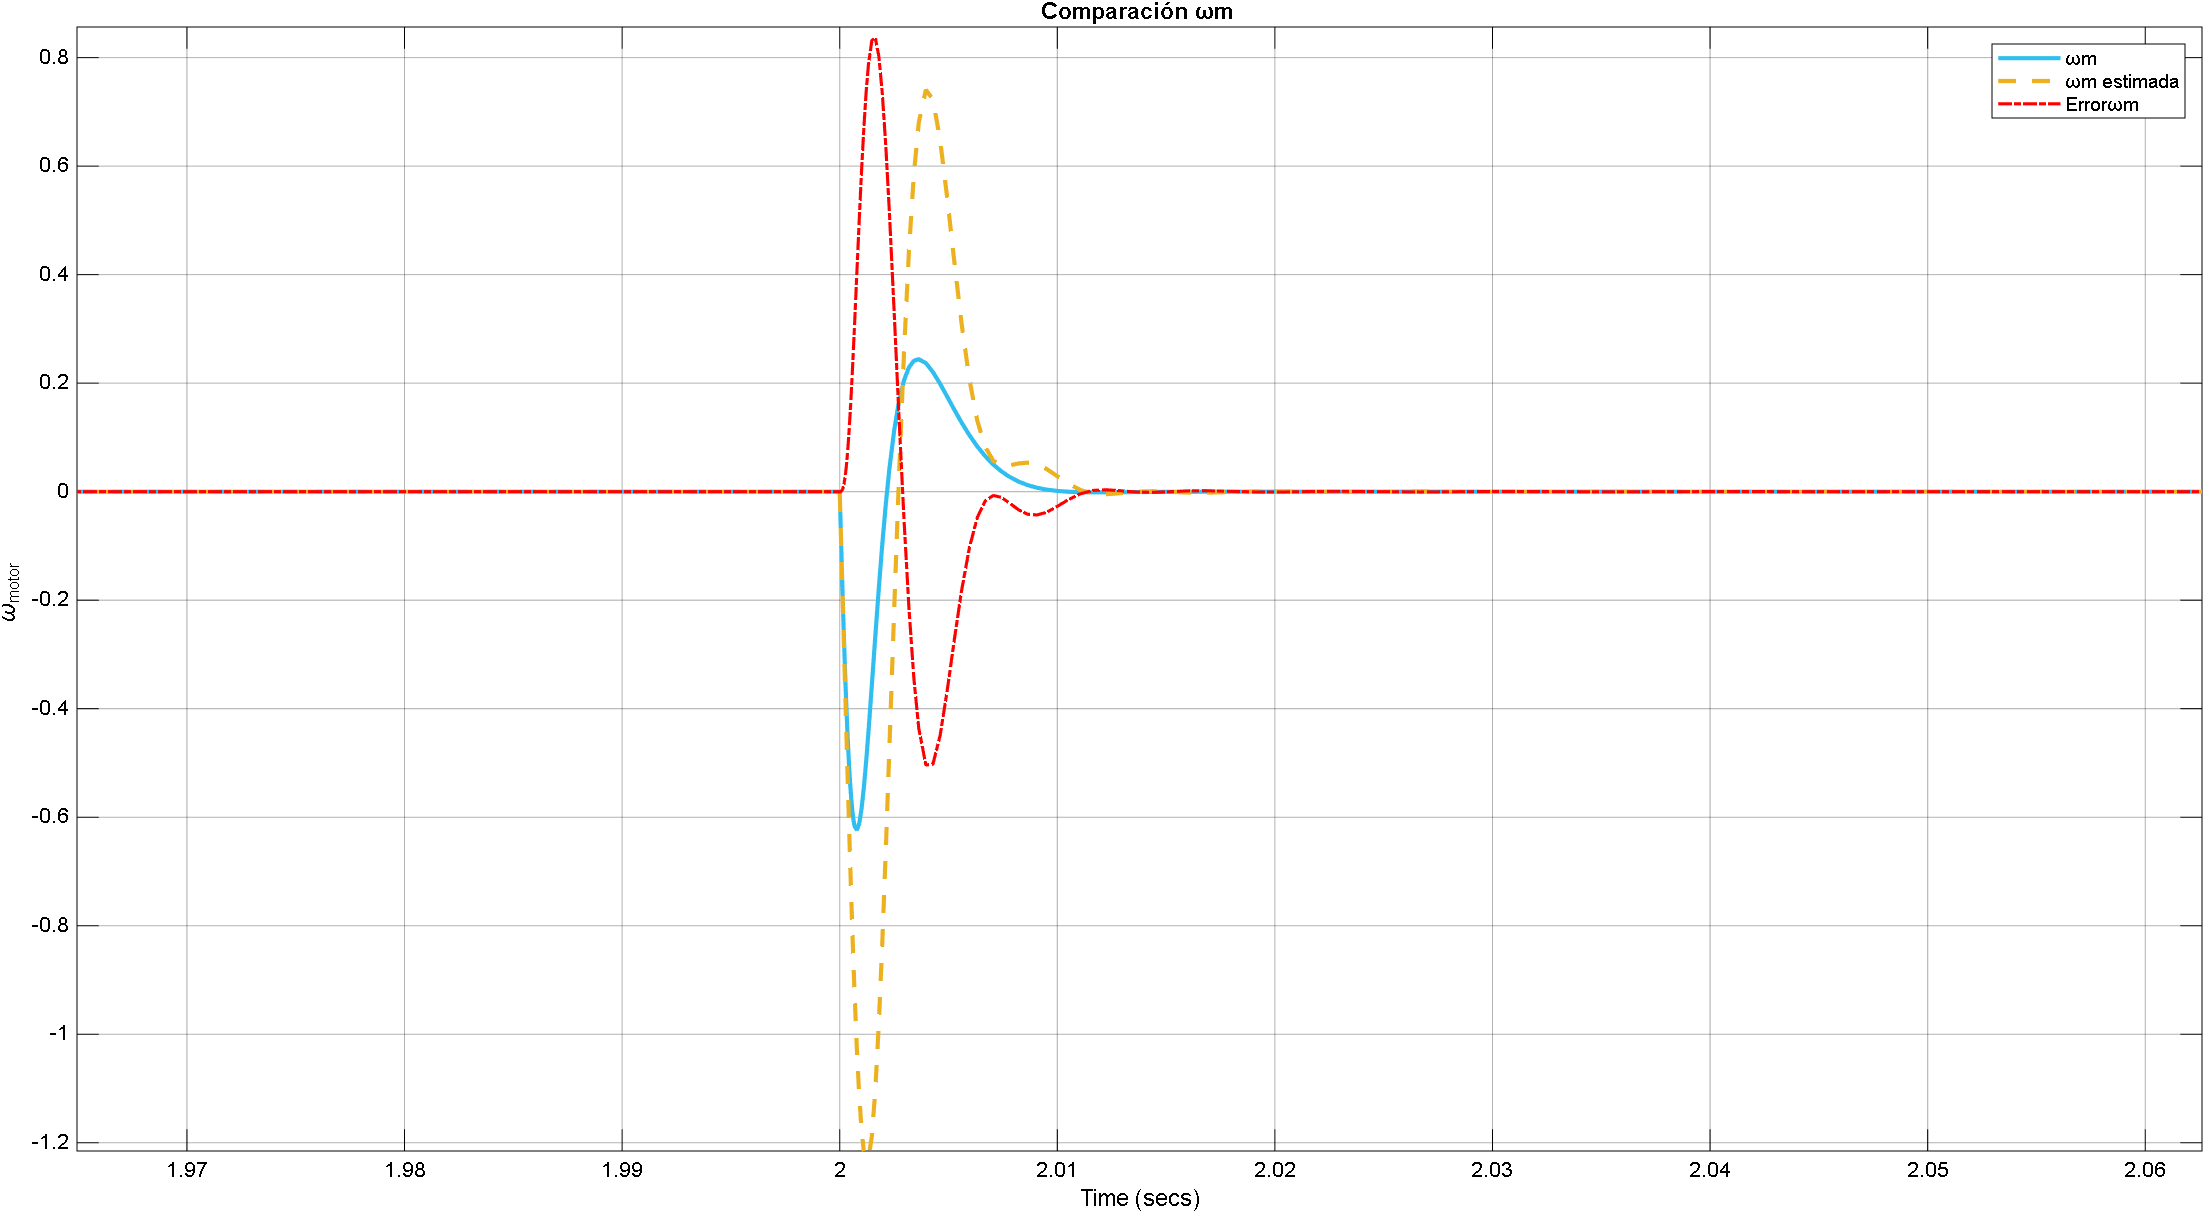
\includegraphics[width=0.86\linewidth,height=0.40\textheight,keepaspectratio]{attachments/DETALLE comparacion estimacion velocidad angulan con perturbacion.png}
    \caption{DETALLE Comparación de $\omega_m$ entre los modelos con y sin estimación debido a la perturbación en torque $T_{ld}$}
    \label{fig:DETALLE comparacion estimación velocidad angular con perturbacion de torque}
\end{figure}
\begin{figure}[!htbp]
    \centering
    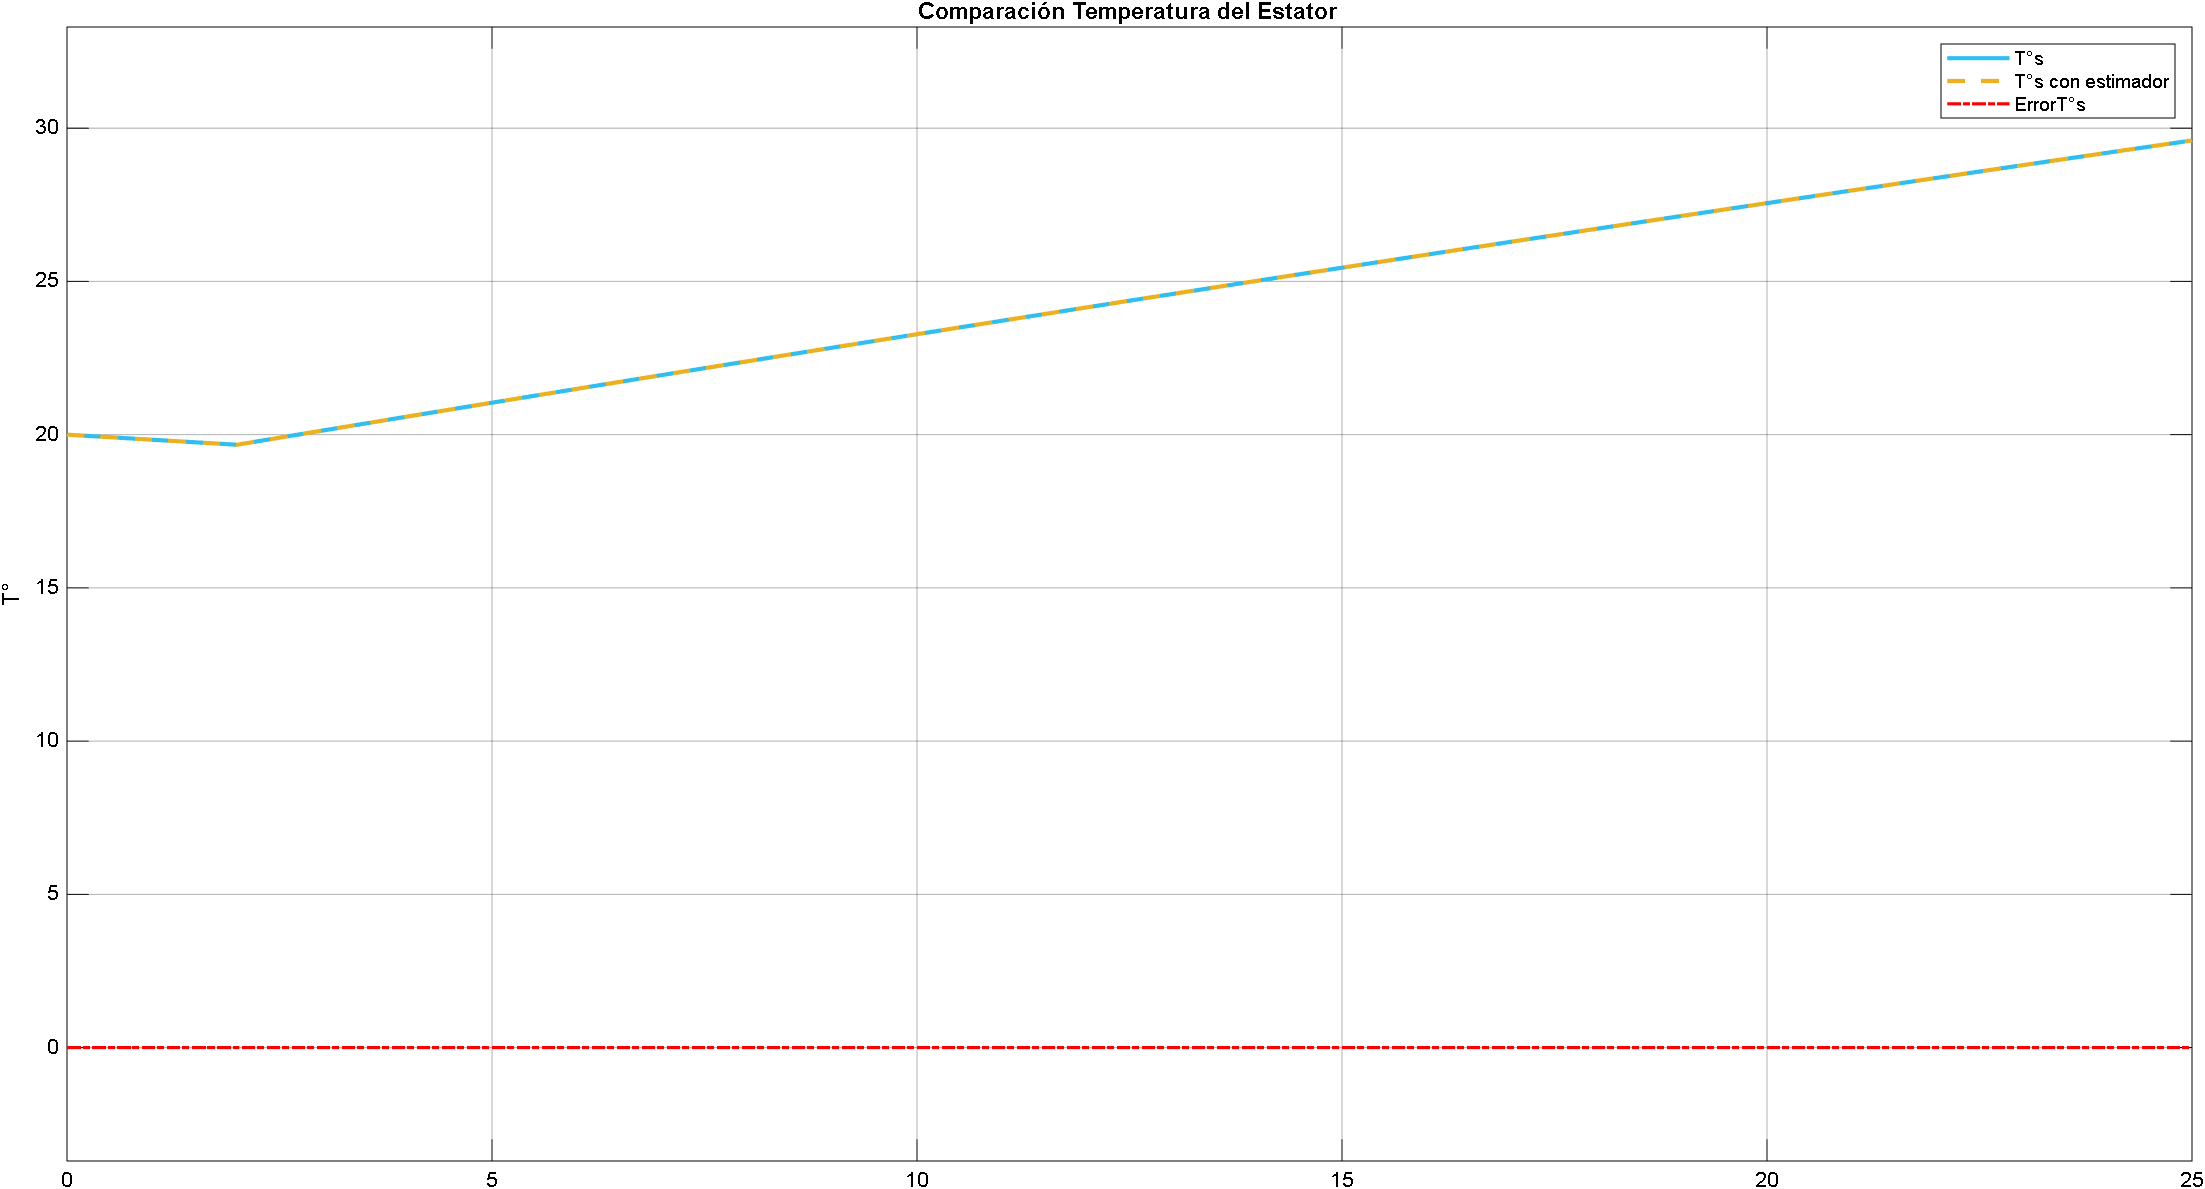
\includegraphics[width=0.86\linewidth,height=0.40\textheight,keepaspectratio]{attachments/comparacion estimacion temperatura del estator con perturbacion.png}
    \caption{Comparación de $T_s$ entre los modelos con y sin estimación debido a la perturbación en torque $T_{ld}$}
    \label{fig:comparacion estimación temperatura del estator con perturbacion de torque}
\end{figure}

\begin{figure}[!htbp]
    \centering
    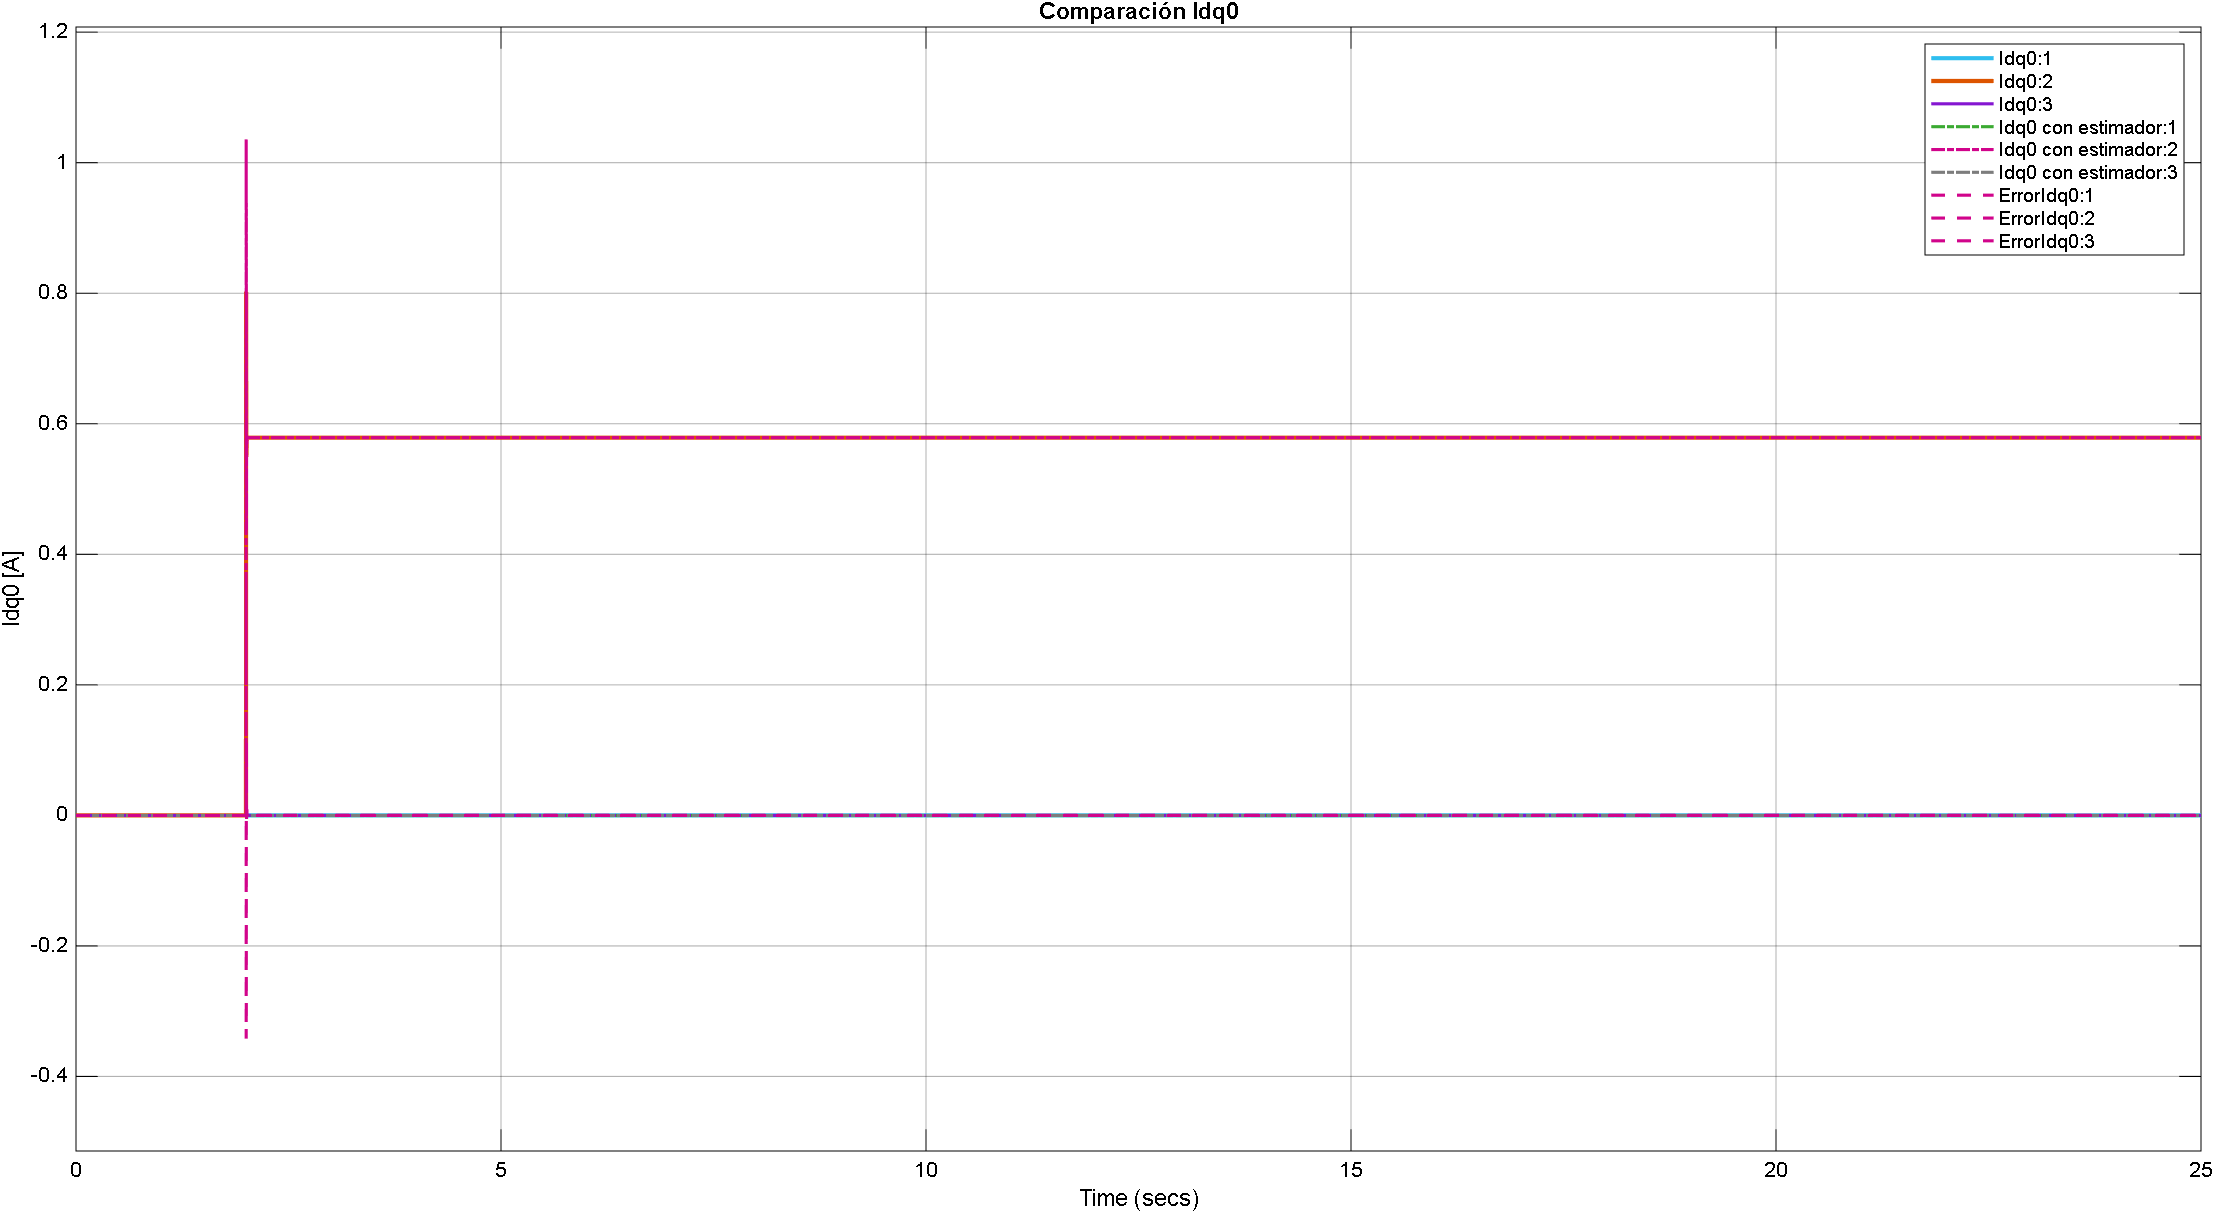
\includegraphics[width=0.86\linewidth,height=0.40\textheight,keepaspectratio]{attachments/comparacion estimacion corriente Idq0 con perturbacion.png}
    \caption{Comparación de $i_{dq0}$ entre los modelos con y sin estimación debido a la perturbación en torque $T_{ld}$}
    \label{fig:comparación estimación idq0 con perturbacion}
\end{figure}
Es posible identificar que en el instante de aplicación de la perturbación el rotor experimenta una deflexión angular transitoria mínima, en régimen permanente éste error es mínimo gracias a la acción integral del control PID de movimiento. De forma similar ocurre en la velocidad angular que gana velocidad al aplicarse la perturbación pero luego de poco más de $10mS$ retorna a la consigna nula.
Justo al momento de aplicación del escalón en la corriente $i_{qs}^r$ es posible ver un picos de corriente la cuál se estabiliza en un valor constante para estabilizar la perturbación constante en régimen permanente. La corriente $i_{ds}^r$ se comporta de manera similar pero con valores prácticamente nulos.
\subsection{Verificación de desempeño y/o mejoras:
}
\subsubsection{Verificar Especificaciones de operación }
A continuación, se realiza la comparación entre los limites de operación establecidos para los
componentes del sistema físico y los valores obtenidos para las simulaciones efectuadas hasta
el momento en la sección \ref{subsubsec:seguimiento consigna movimiento} 
\begin{table}[!htbp]
    \centering
    \small
    \caption{Valores de operación frente a valores obtenidos en simulación.}
    \label{tab:verificacion-operacion}
    \begin{tabular}{l c c c c}
        \toprule
        \multirow{2}{*}{\textbf{Especificación}} & \multicolumn{2}{c}{\textbf{Especificación de Operación}} & \multicolumn{2}{c}{\textbf{Valores de Simulación}} \\
        \cmidrule(lr){2-3} \cmidrule(lr){4-5}
         & Régimen Continuo & Valor Pico & Régimen Continuo & Valor Pico \\
        \midrule
        Torque (Caja) & $17,0\;\mathrm{N\,m}$ & $45.0\;\mathrm{N\,m}$ & $\;\mathrm{0.03N\,m}$ & $\;\mathrm{6.9N\,m}$ \\
        Velocidad Angular (Motor) & $691.15\;\mathrm{rad\,s^{-1}}$ & $691,15\;\mathrm{rad\,s^{-1}}$ & $\dots\;\mathrm{rad\,s^{-1}}$ & $209\;\mathrm{rad\,s^{-1}}$ \\
        Corriente (Estator) & $0.4\;\mathrm{A}$ & $2.0\;\mathrm{A}$ & $0\;\mathrm{A}$ & $95.76\;\mathrm{A}$ \\
        Tensión de Fase (Estator) & $17.32\;\mathrm{V}$ & $24.49\;\mathrm{V}$ & $0\;\mathrm{V}$ & $2248.9\;\mathrm{V}$ \\
        Temperatura (Estator) & $115,0\;^\circ\mathrm{C}$ & $115,0\;^\circ\mathrm{C}$ & $69.8\;^\circ\mathrm{C}$ & $\dots\;^\circ\mathrm{C}$ \\
        \bottomrule
    \end{tabular}
\end{table}
Al evaluar el cuadro es posible apreciar que se exceden ciertos valores de operación tales como voltaje y corriente. Esto es debido a los cambios bruscos de derivada en la posición, lo cual implica aceleraciones de gran magnitud. Es posible contrarrestar esta situación suavizando las transiciones de una derivada a otra en la consigna de movimiento, este suavizado se hará con la intensión de conseguir una curva de velocidad más suave. 
A continuación se ve la nueva consigna suavizada:
\begin{figure}[!htbp]
    \centering
    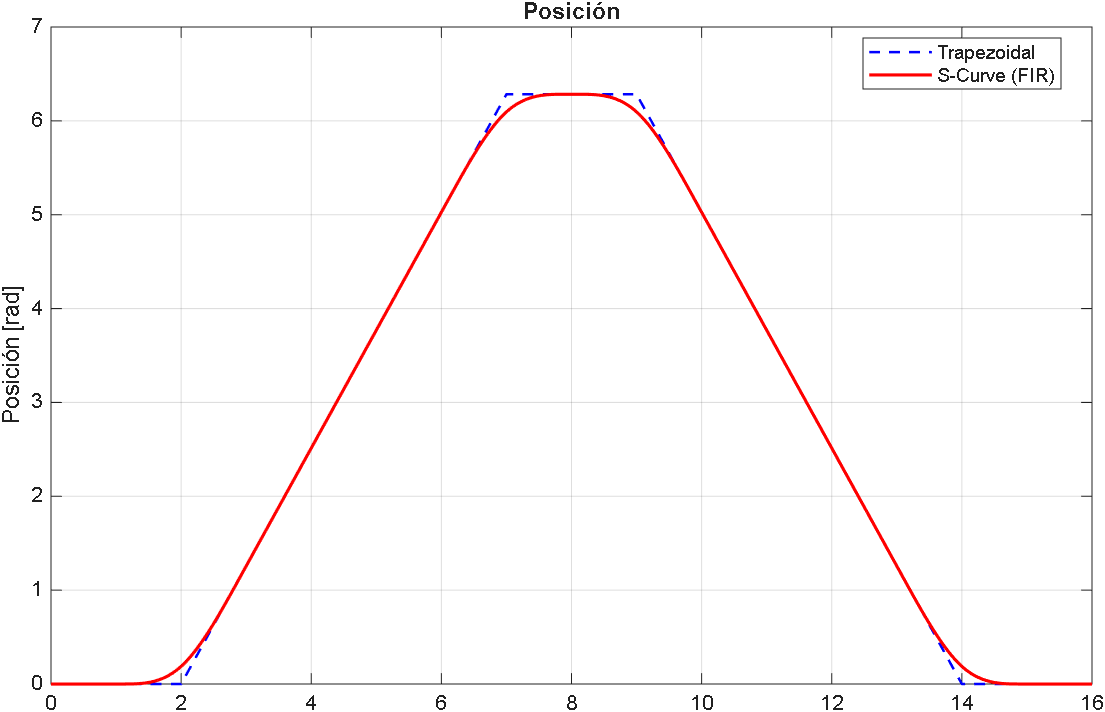
\includegraphics[width=0.64\linewidth,height=0.26\textheight,keepaspectratio]{attachments/Consigna de movimiento suavizada.png}
    \caption{Referencia de posición de la carga. Comparación entre la consigna trapezoidal y la consigna suavizada.}
    \label{fig:connsigna movimiento suavizada}
    \par\medskip
    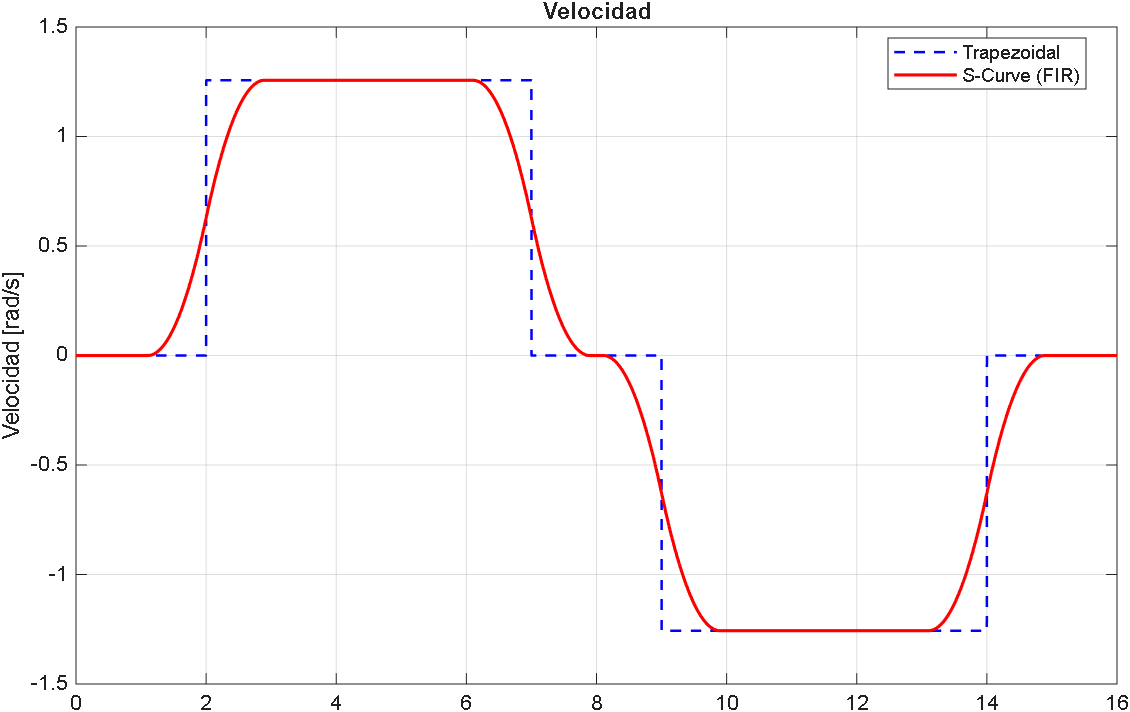
\includegraphics[width=0.64\linewidth,height=0.26\textheight,keepaspectratio]{attachments/Consigna de velocidad suavizada.png}
    \caption{Referencia de velocidad de la carga. Comparación entre la consigna trapezoidal y la consigna suavizada.}
    \label{fig:connsigna velocidad suavizada}
\end{figure}
Ya conociendo la nueva consigna se evalúa que con ese cambio se cumpla con las especificaciones de operación 

\begin{figure}[!htbp]
    \centering
    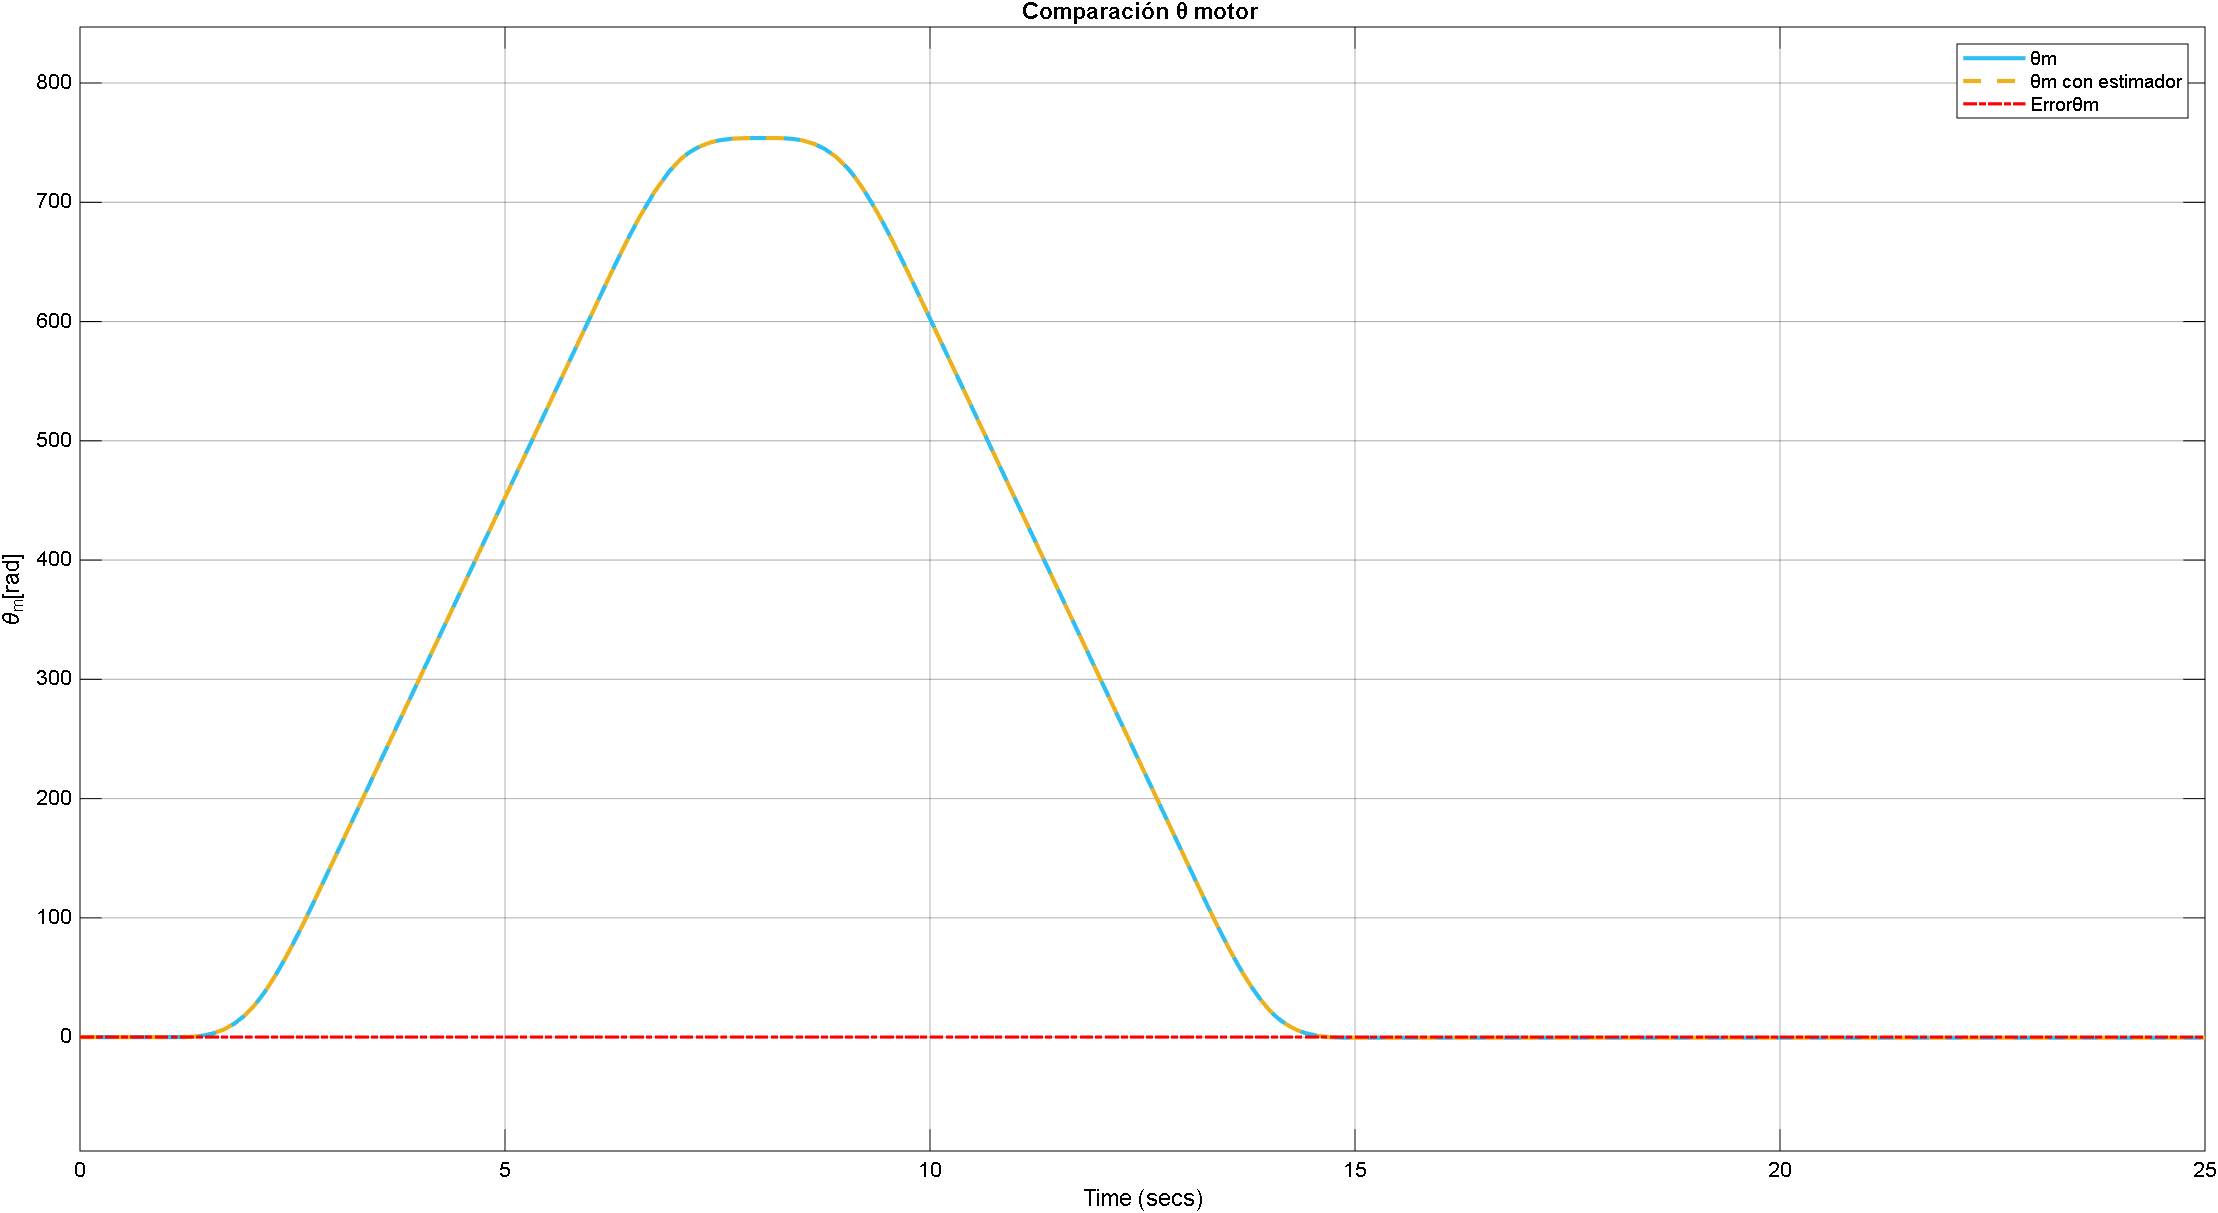
\includegraphics[width=0.86\linewidth,height=0.40\textheight,keepaspectratio]{attachments/posicion angular consigna suavizada.png}
    \caption{Posición angular $\theta_m$ con consigna trapezoidal suavizada}
    \label{fig:posicion angular con consigna suavizada}
    \par\medskip
    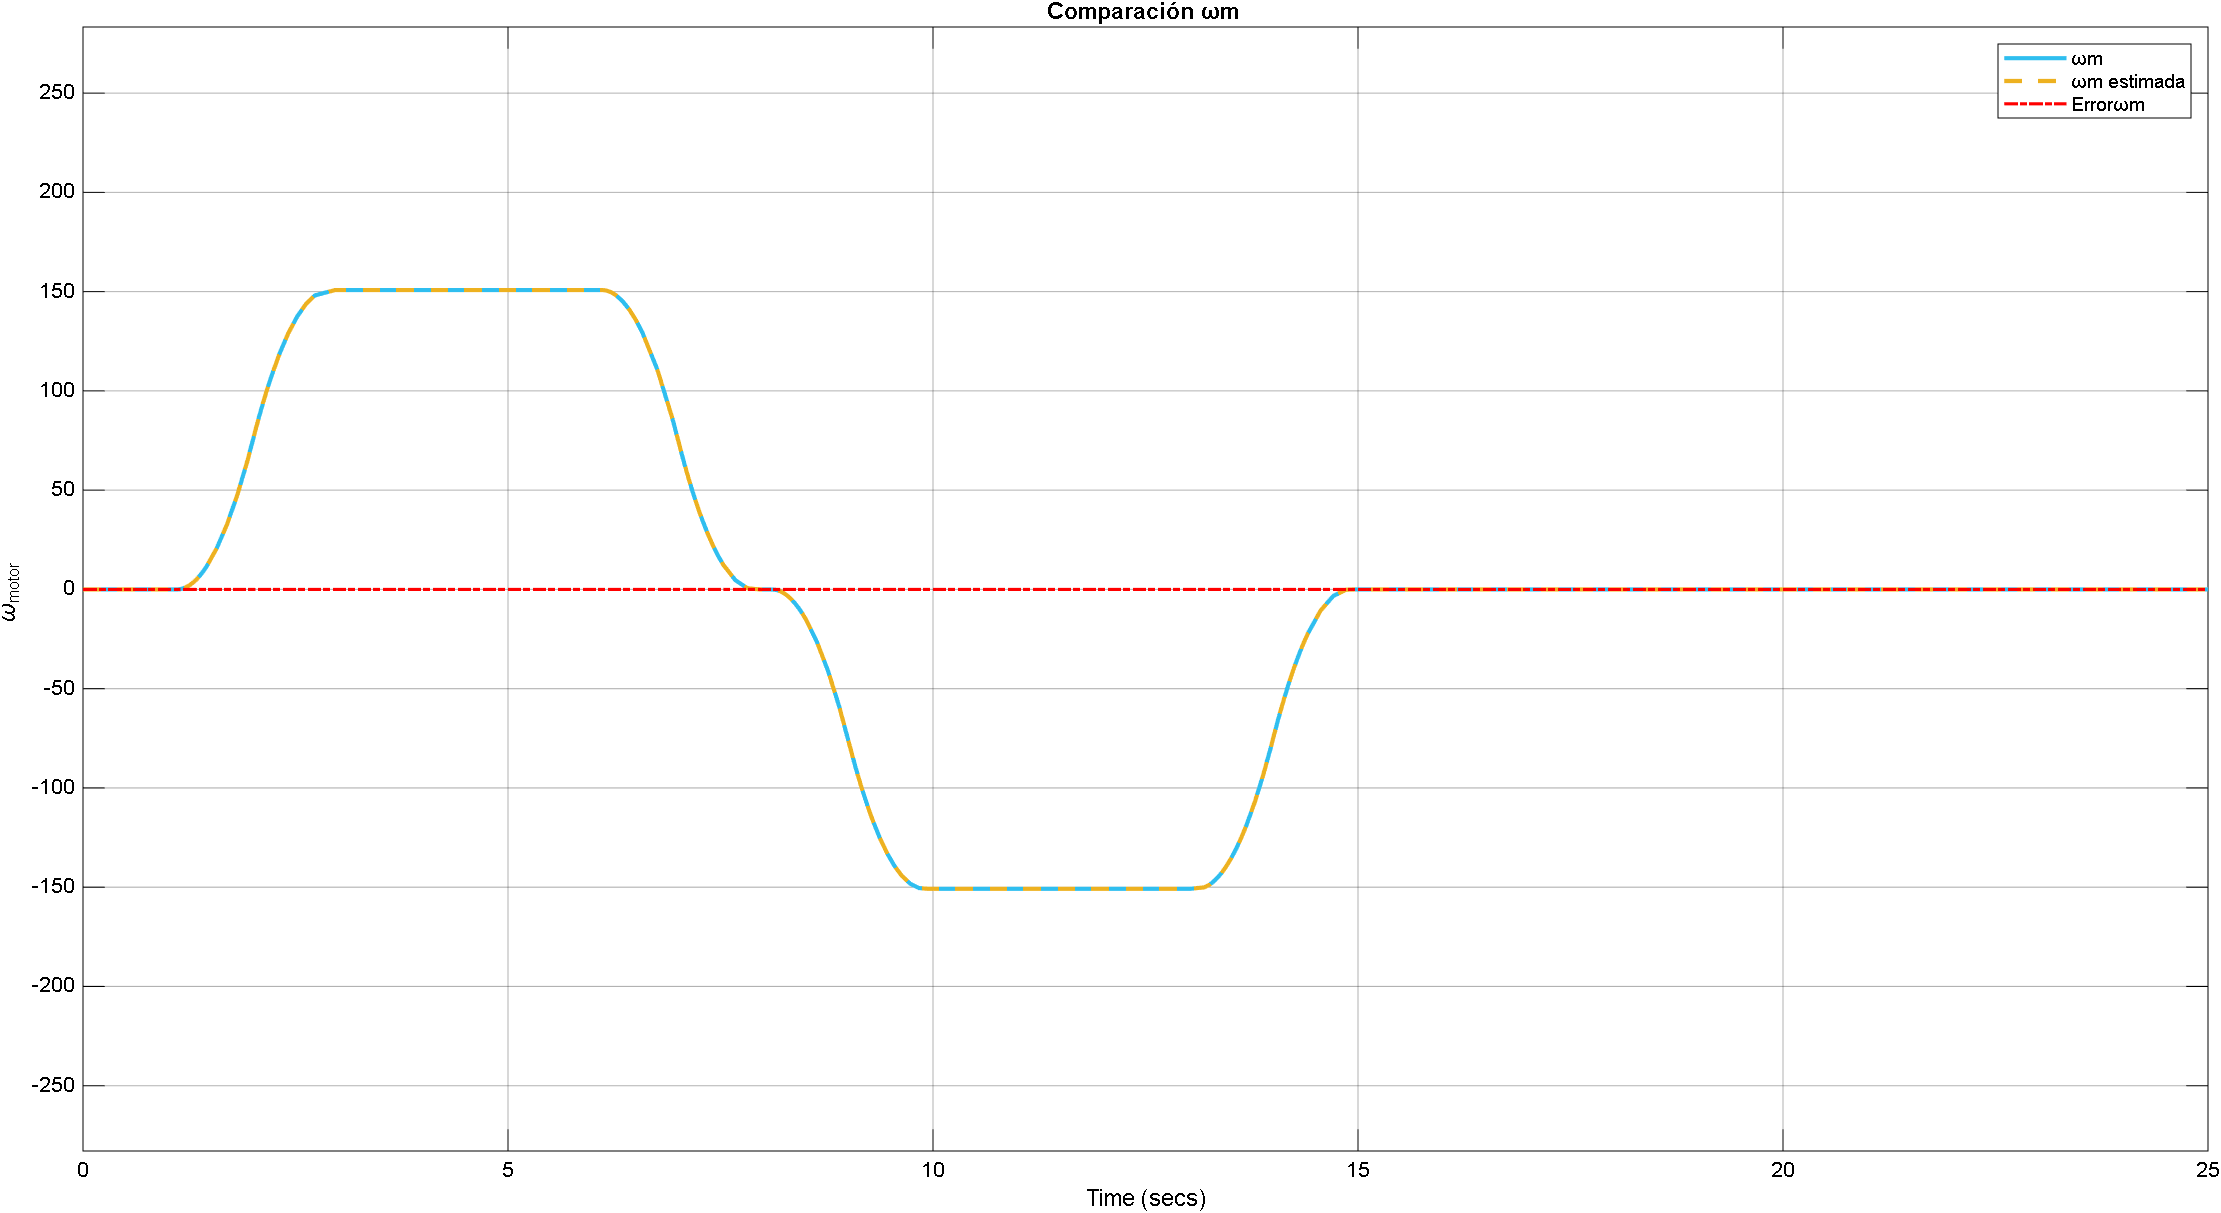
\includegraphics[width=0.86\linewidth,height=0.40\textheight,keepaspectratio]{attachments/velocidad angular consigna suavizada.png}
    \caption{Velocidad angular $\omega_m$ con consigna trapezoidal suavizada}
    \label{fig:velocidad angular con consigna suavizada}
\end{figure}
\begin{figure}[!htbp]
    \centering
    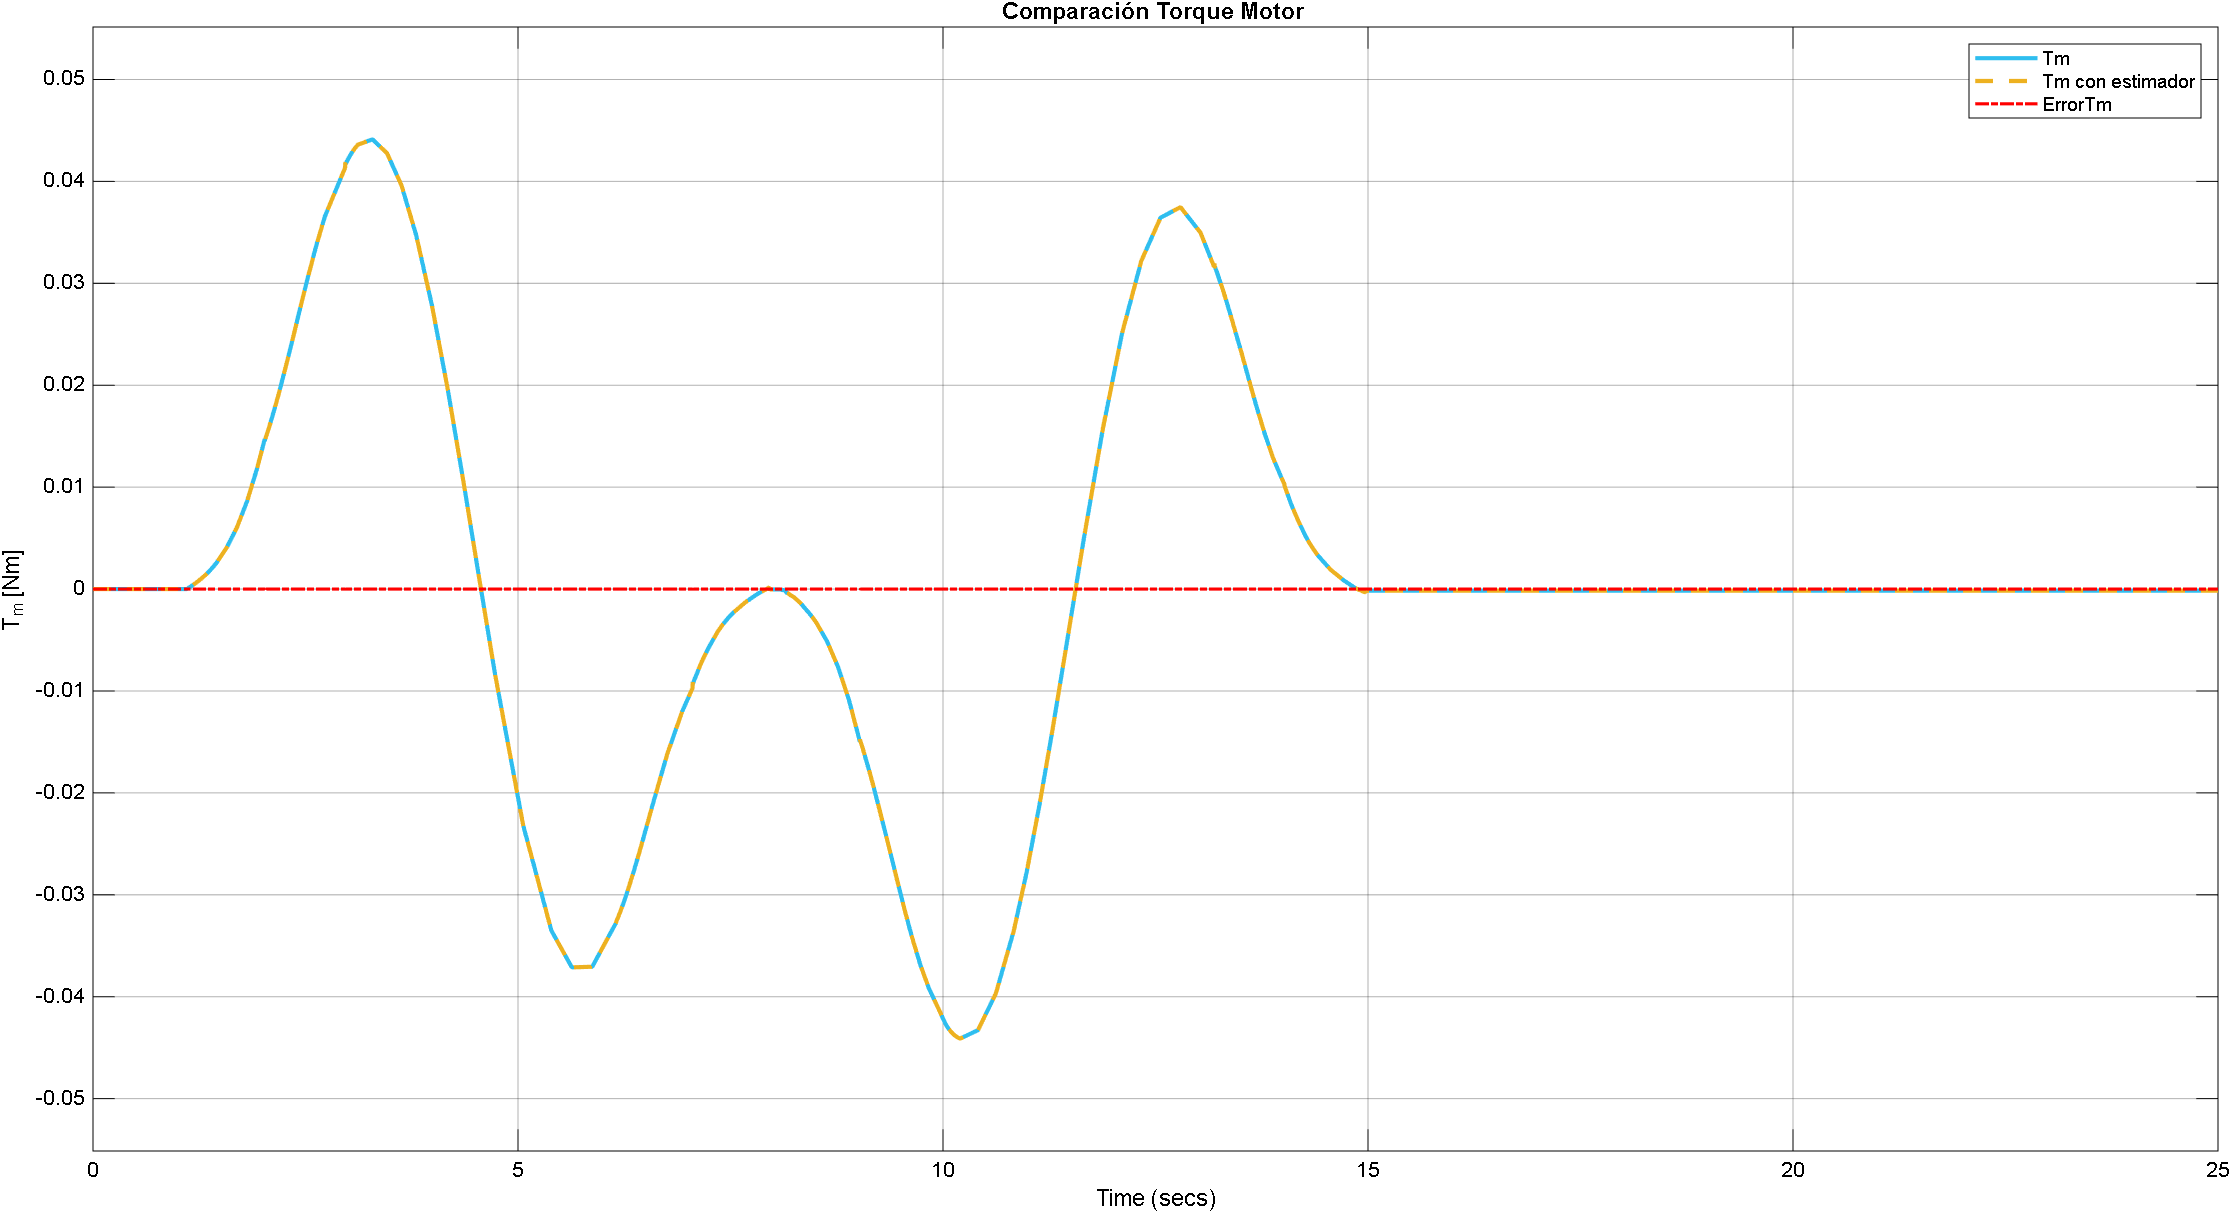
\includegraphics[width=0.86\linewidth,height=0.40\textheight,keepaspectratio]{attachments/torque motor consigna suavizada.png}
    \caption{Torque motor $T_m$ con consigna trapezoidal suavizada}
    \label{fig:torque motor con consigna suavizada}
    \par\medskip
    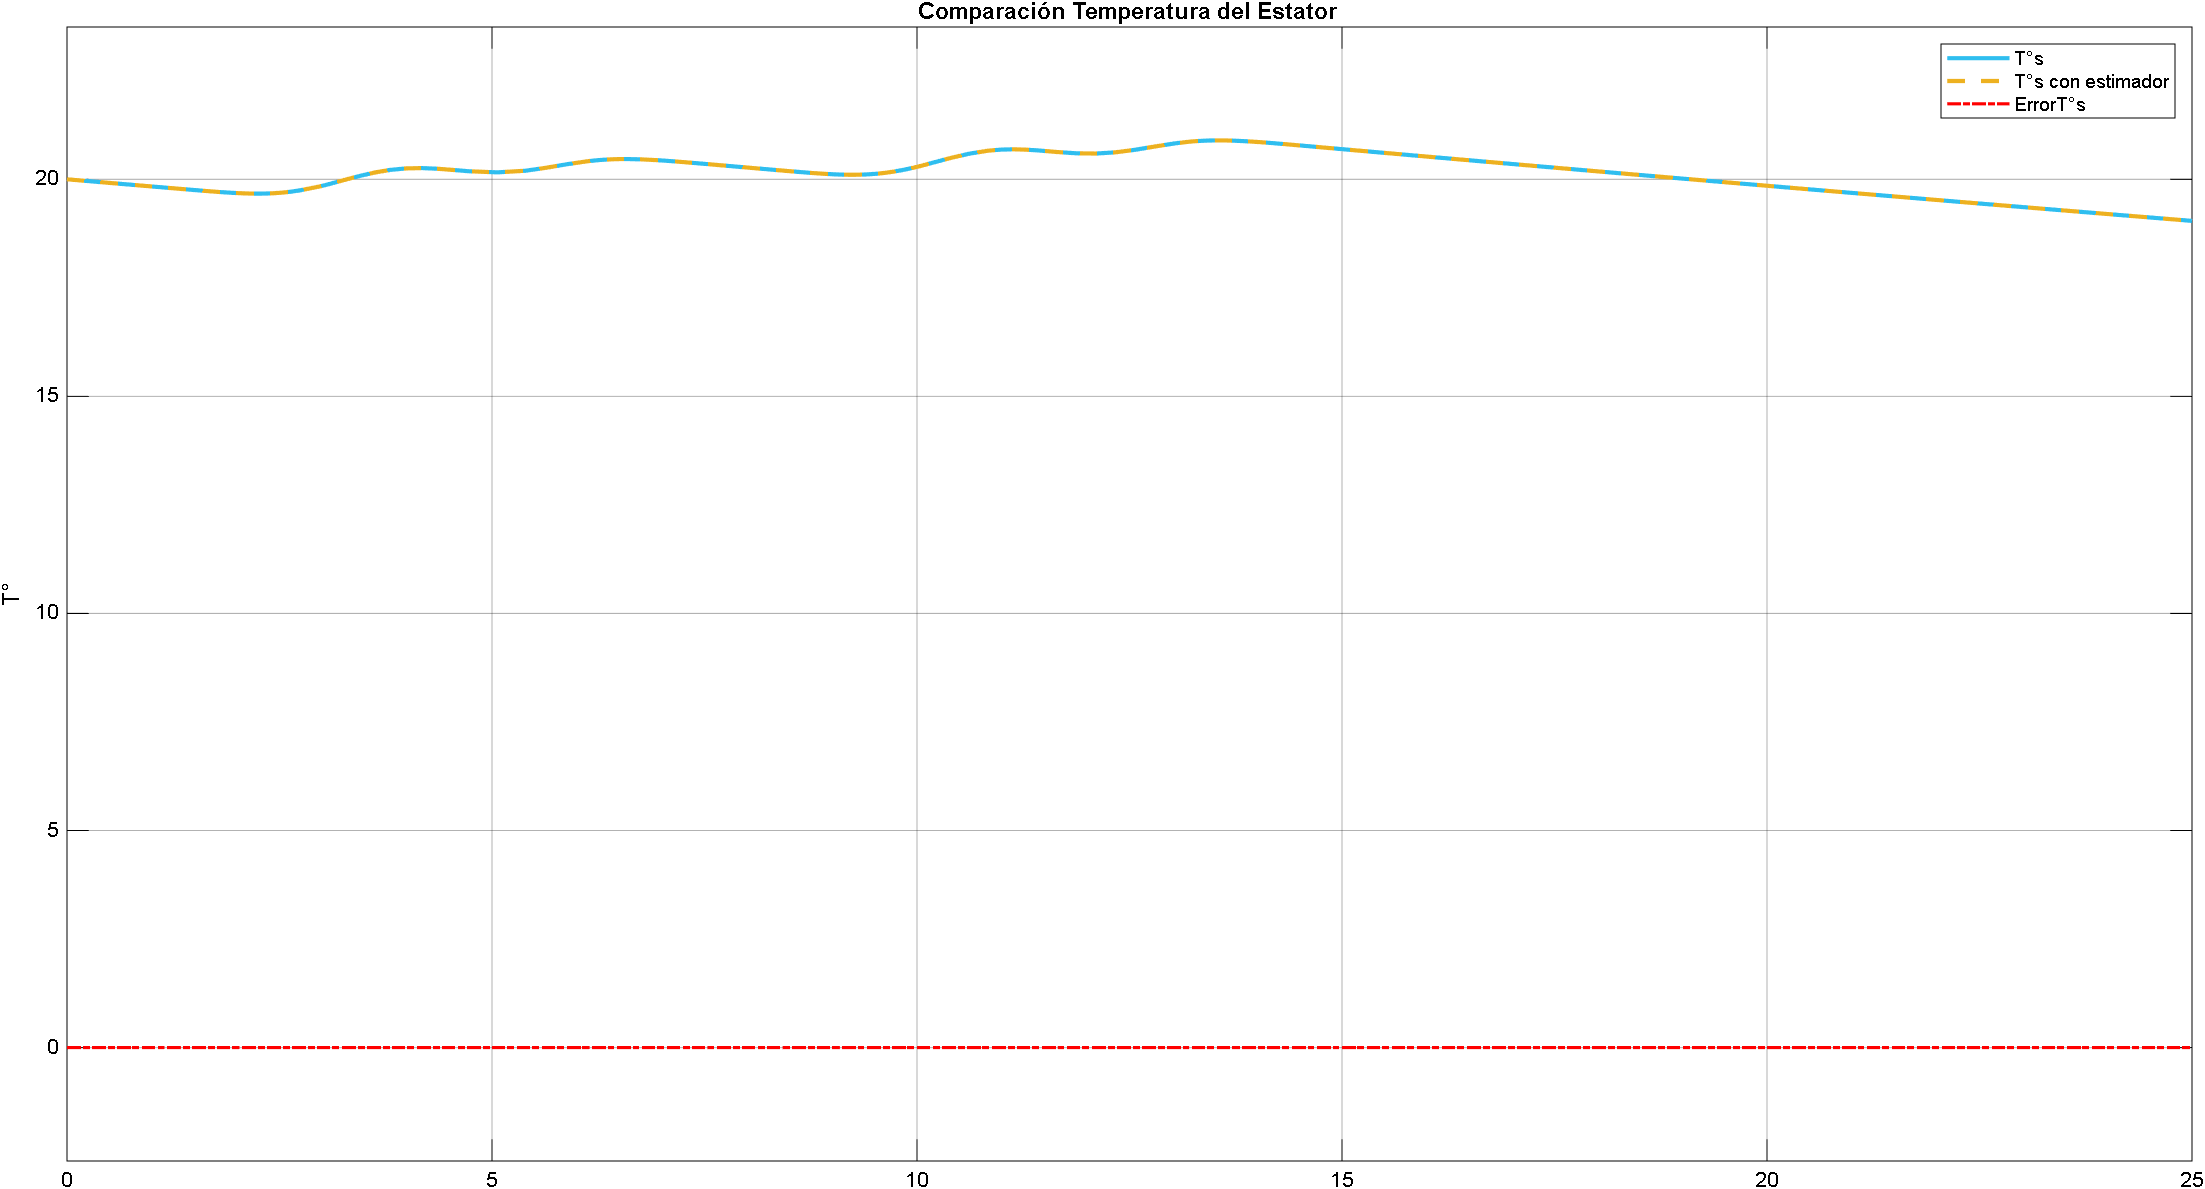
\includegraphics[width=0.86\linewidth,height=0.40\textheight,keepaspectratio]{attachments/temperatura estator consigna suavizada.png}
    \caption{Temperatura del estator $T_{s}^\circ$ con consigna trapezoidal suavizada}
    \label{fig:temperatura del estator con consigna suavizada}
\end{figure}
\begin{figure}[!htbp]
    \centering
    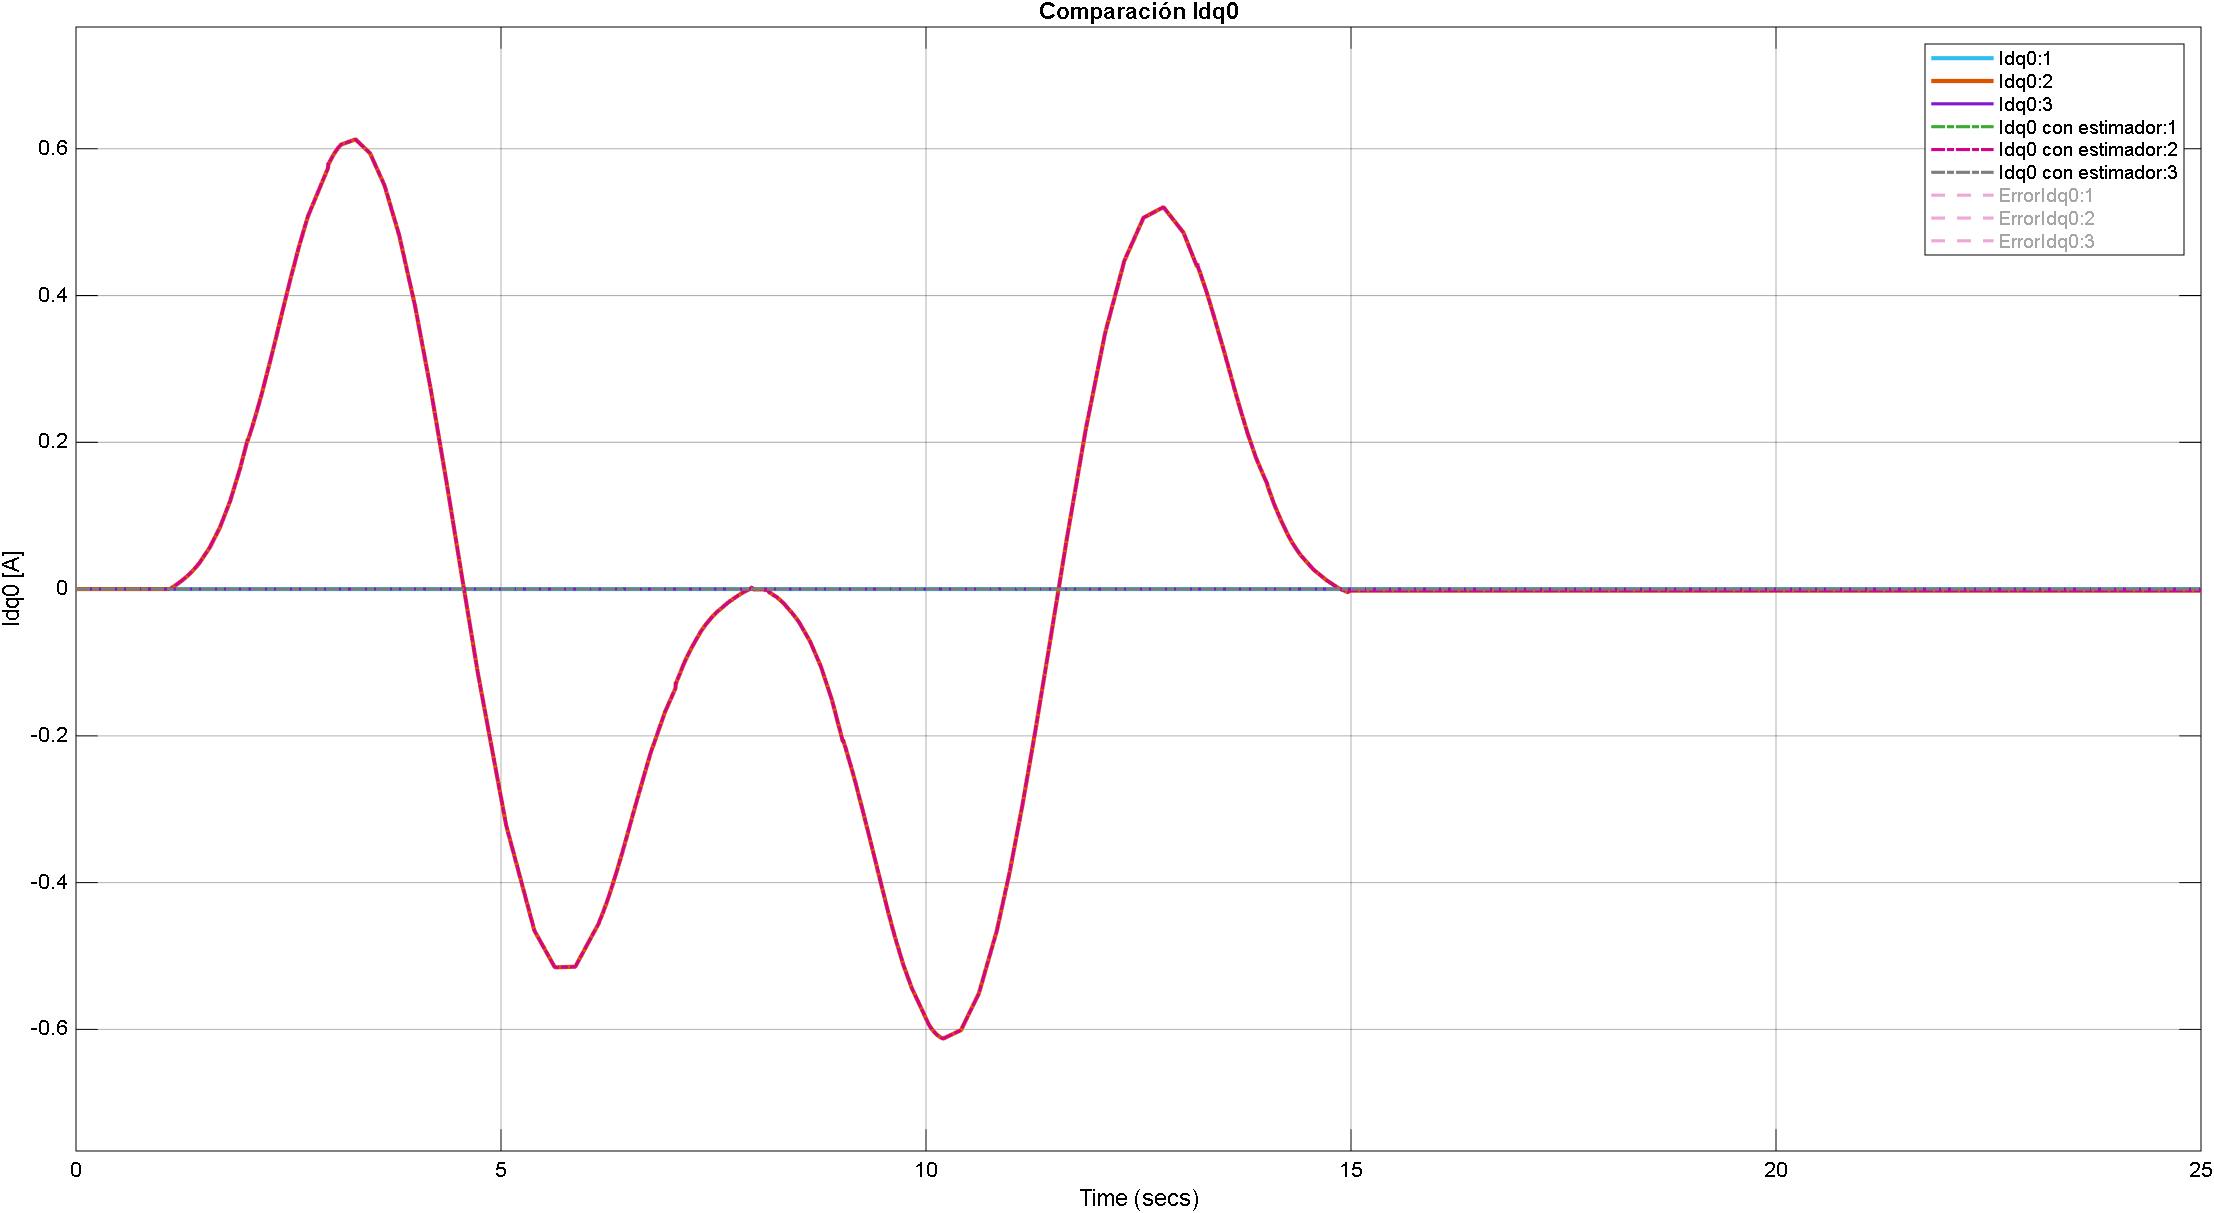
\includegraphics[width=0.88\linewidth,height=0.40\textheight,keepaspectratio]{attachments/Idq0 consigna suavizada.png}
    \caption{Corrientes virtuales $i_{dq0}^r$ con consigna trapezoidal suavizada}
    \label{fig:corriente virtual con consigna suavizada}
    \par\medskip
    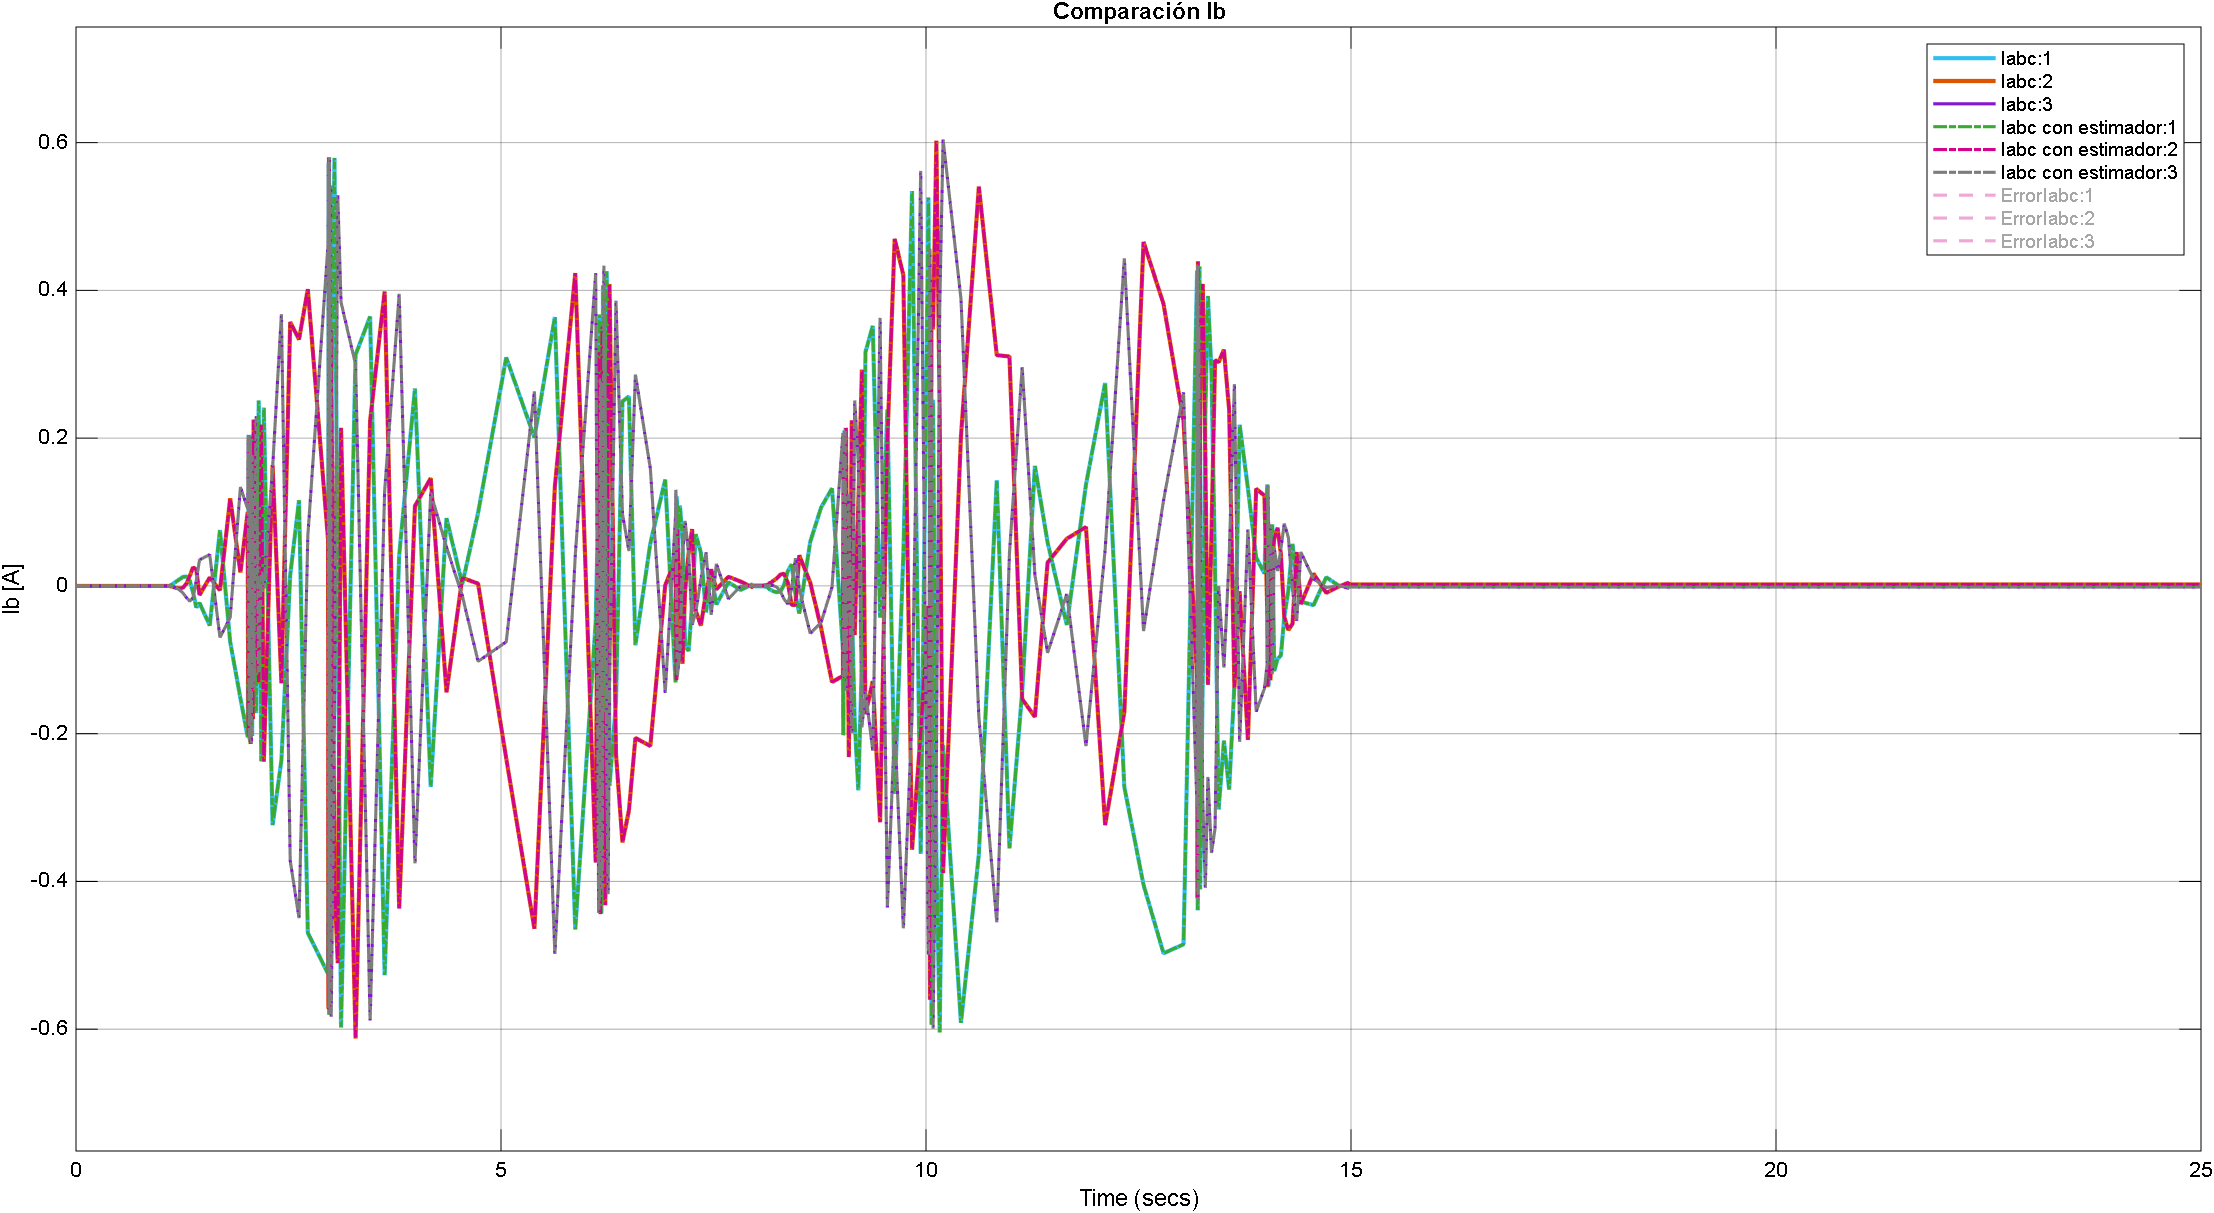
\includegraphics[width=0.88\linewidth,height=0.40\textheight,keepaspectratio]{attachments/Iabc consigna suavizada.png}
    \caption{Corrientes reales $i_{abc}$ con consigna trapezoidal suavizada}
    \label{fig:corriente reales con consigna suavizada}
\end{figure}
\begin{figure}[!htbp]
    \centering
    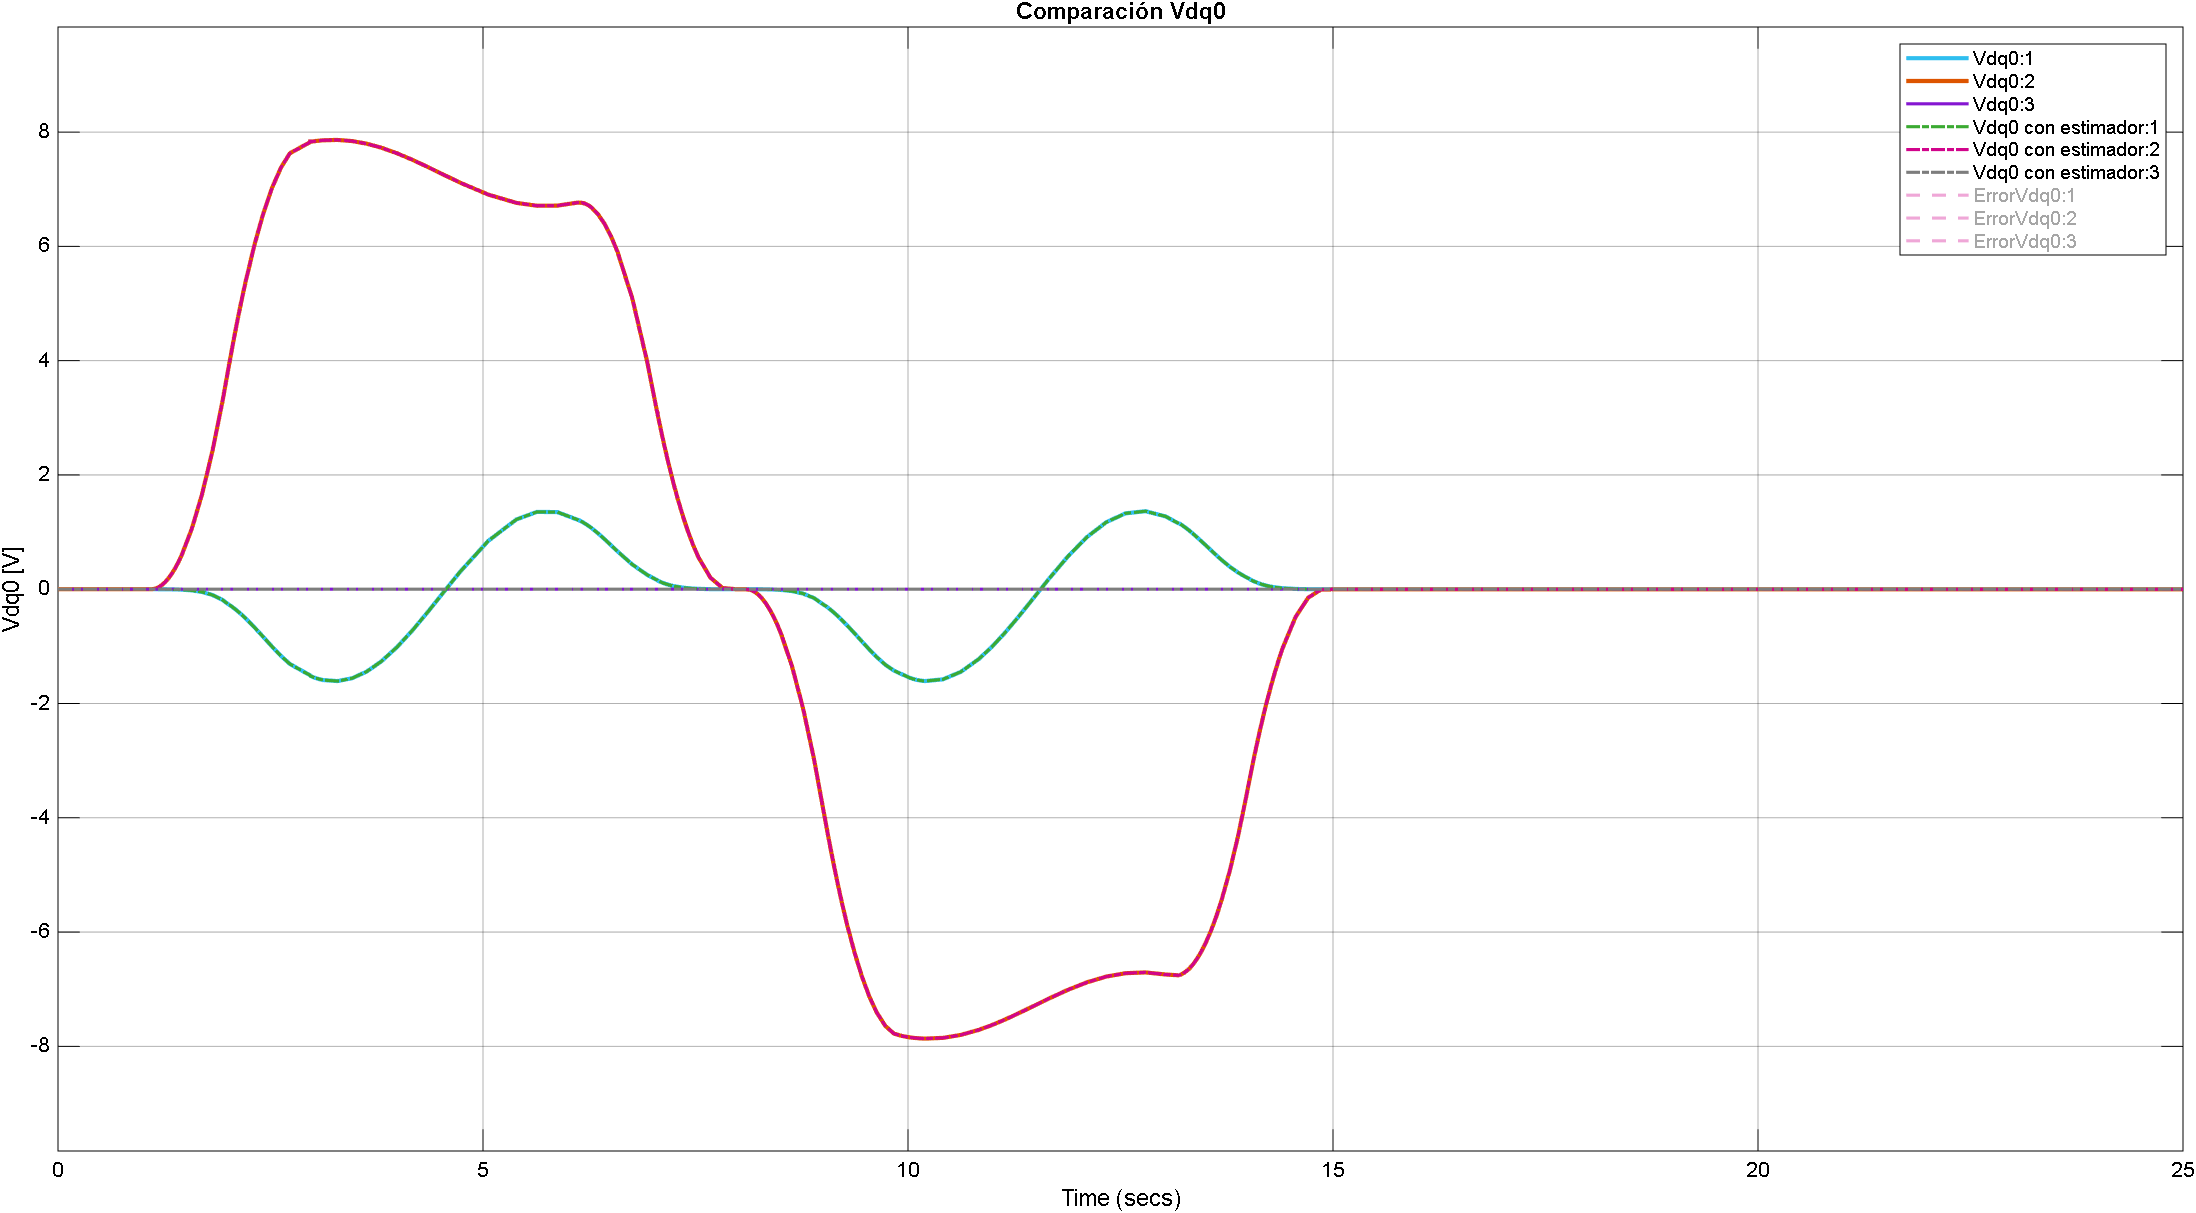
\includegraphics[width=0.88\linewidth,height=0.40\textheight,keepaspectratio]{attachments/Vdq0 consigna suavizada.png}
    \caption{Tensiones virtuales $v_{dq0}^r$ con consigna trapezoidal suavizada}
    \label{fig:tensiones virtuales con consigna suavizada}
    \par\medskip
    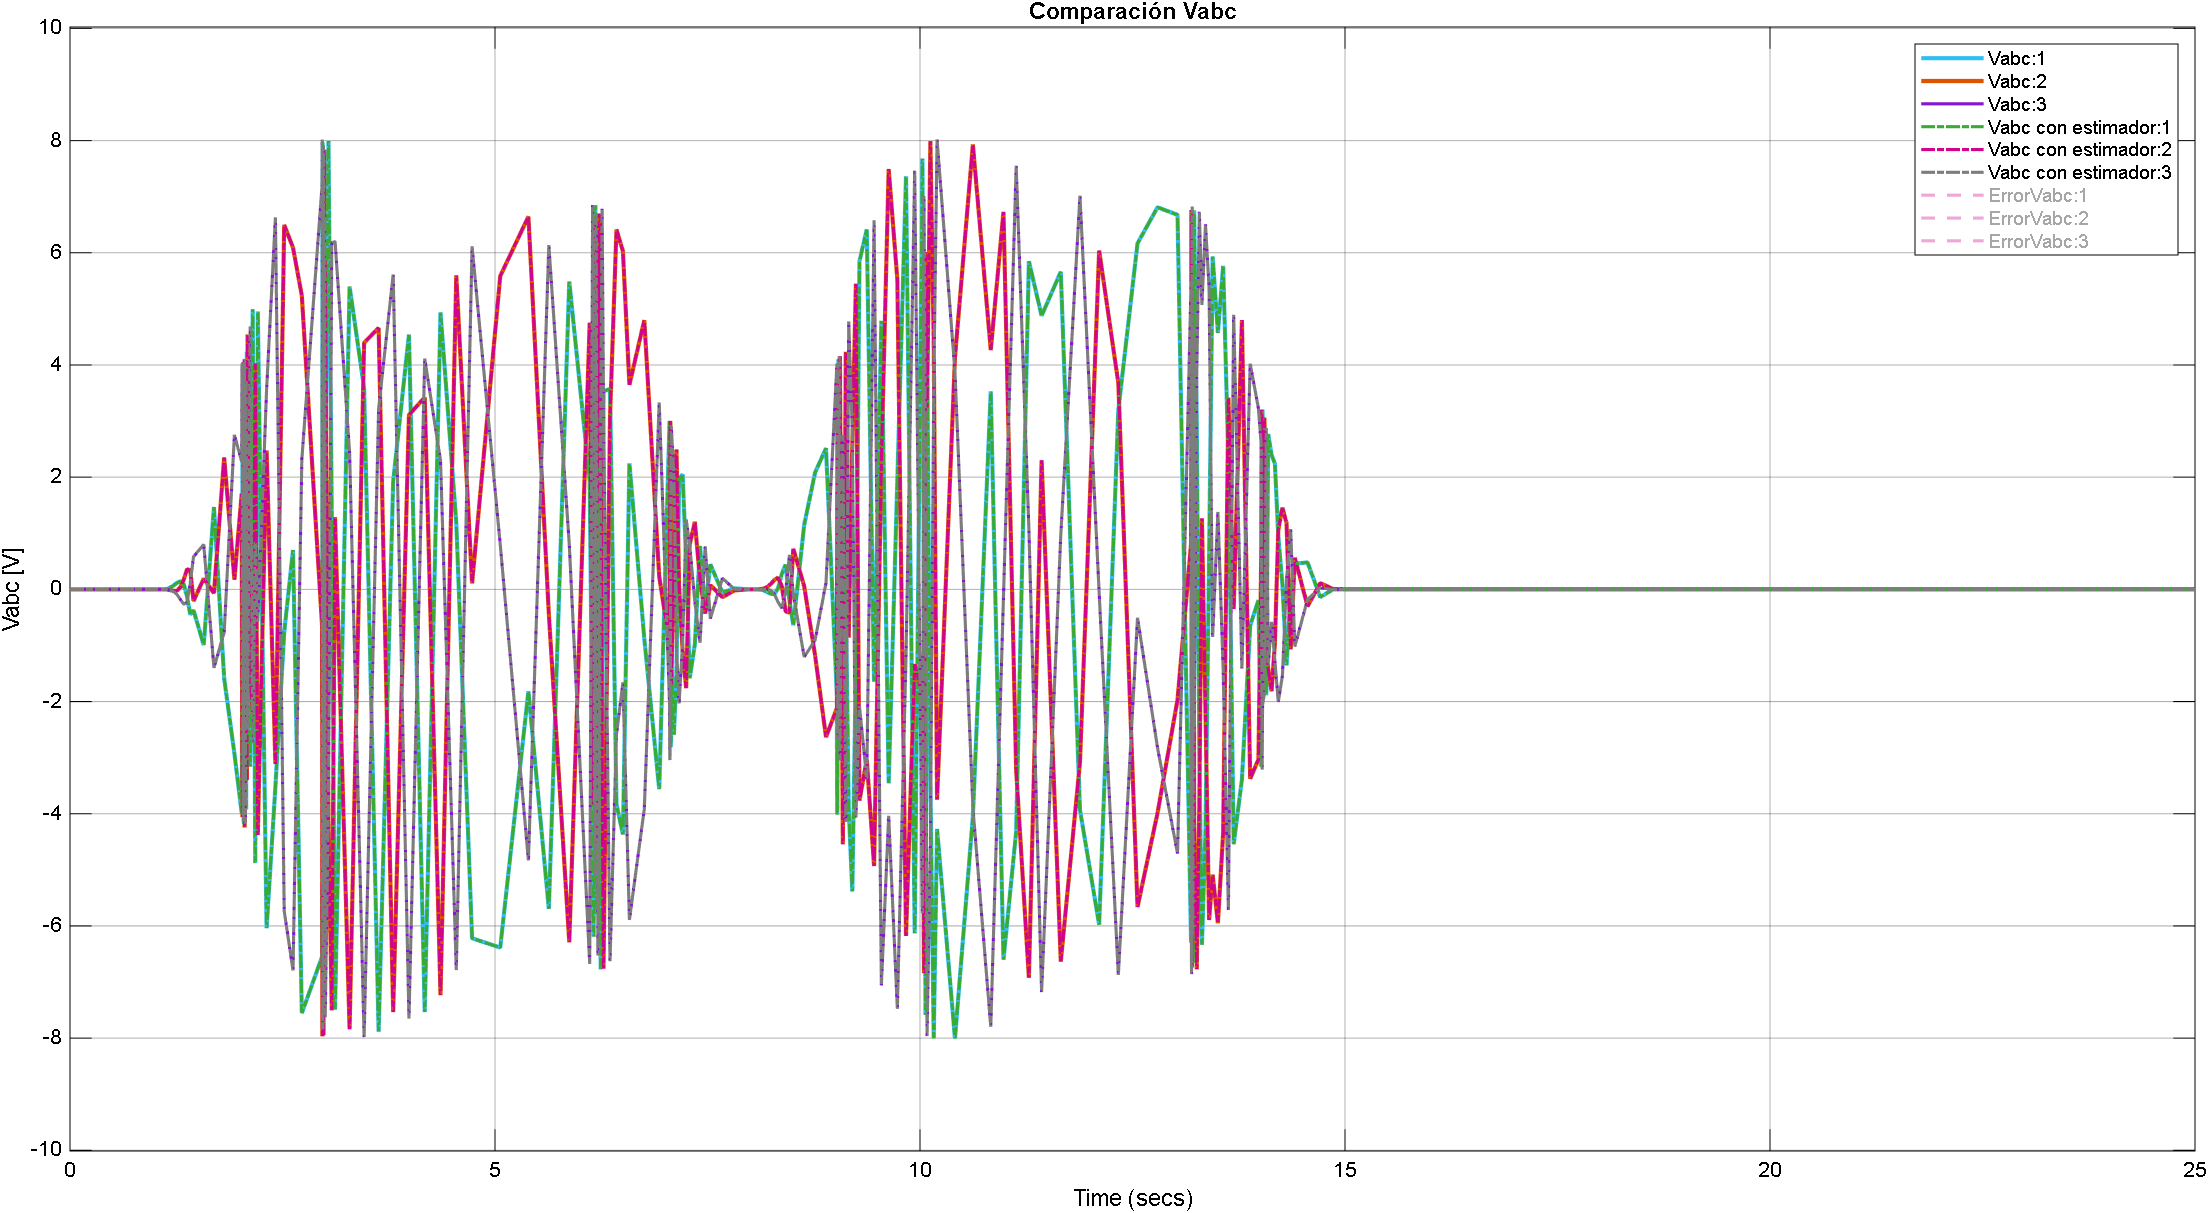
\includegraphics[width=0.88\linewidth,height=0.40\textheight,keepaspectratio]{attachments/Vabc consigna suavizada.png}
    \caption{Tensiones de fase $v_{abc}$ con consigna trapezoidal suavizada}
    \label{fig:tensiones reales con consigna suavizada}
\end{figure}
Se ve que suavizar la consigna permitió que los parámetros problemáticos se encuentren dentro de los rangos operativos.

\subsubsection{Acción integral en el observador}
En la sección \ref{subsubsec: rechazo a perturbaciones} durante las simulaciones se evidenció la presencia de un error en régimen permanente ante la aplicación de la perturbación $T_{ld}$. Con la intensión de eliminar o disminuir este error, se busca incorporar una acción de tipo integral a la estructura del observador de estados previamente formulado.

Se sigue trabajando con el diseño que se inició previamente \ref{subsec:observador de estado de orden reducido}, donde se diseñó un observador de estado de orden reducido 
considerando las compensaciones por retroalimentación no lineal introducidas en el modulador de torque.
\ref{eq:observador-mecanico}

Para anular el error de régimen permantente ante una perturbación constante ya mencionado, se expande el vector de estados del observador incorporando una variable acumulativa $\hat{v}(t)$, que corresponde a la integral del error de estimación angular:
\begin{equation}
\mathbf{z}(t) = \begin{bmatrix} \theta_m(t) \\ \omega_m(t) \\ v(t) \end{bmatrix}, \qquad
\hat{\mathbf{z}}(t) = \begin{bmatrix} \hat{\theta}_m(t) \\ \hat{\omega}_m(t) \\ \hat{v}(t) \end{bmatrix}
\end{equation}
De modo tal que las ecuaciones diferenciales del observador aumentado quedan expresadas como:
\begin{equation}
\begin{cases}
\dot{\hat{\theta}}_m(t) = \hat{\omega}_m(t) + K_{\theta}\big(\theta_m(t) - \hat{\theta}_m(t)\big) \\
\dot{\hat{\omega}}_m(t) = \dfrac{1}{J_{eq}}T_m^*(t) + \hat{v}(t) + K_{\omega}\big(\theta_m(t) - \hat{\theta}_m(t)\big) \\
\dot{\hat{v}}(t) = K_{i}\big(\theta_m(t) - \hat{\theta}_m(t)\big)
\end{cases}
\end{equation}
La matriz de estado de la dinámica del error $\tilde{\mathbf{z}}(t) = \mathbf{z}(t) - \hat{\mathbf{z}}(t)$ pasa a ser de tercer orden:
\begin{equation}
\mathbf{A}_{\text{obs,aum}} = \begin{bmatrix} -K_{\theta} & 1 & 0 \\ -K_{\omega} & 0 & 1 \\ -K_{i} & 0 & 0 \end{bmatrix}
\end{equation}
Cuyo polinomio característico resulta:
\begin{equation}
P(s) = \det(s\mathbf{I} - \mathbf{A}_{\text{obs,aum}}) = s^3 + K_{\theta}\,s^2 + K_{\omega}\,s + K_{i}
\end{equation}
Ubicando los tres polos reales coincidentes en el mismo valor de diseño original ($|p_{\text{obs}}| = 3200\;\mathrm{rad/s}$):
\begin{equation}
P_{\text{obs}}^*(s) = (s + 3200)^3 = s^3 + 9600\,s^2 + 30,72\times 10^6\,s + 3,2768\times 10^{10}
\end{equation}
Igualando término a término, se obtienen las ganancias del observador aumentado:
\begin{equation}
\begin{cases}
K_{\theta} = 9600\;\mathrm{s^{-1}} \\
K_{\omega} = 3,0720\times 10^7\;\mathrm{s^{-2}} \\
K_{i} = 3,2768\times 10^{10}\;\mathrm{s^{-3}}
\end{cases}
\end{equation}
\par\medskip
\noindent\begin{minipage}{\linewidth}
    \centering
    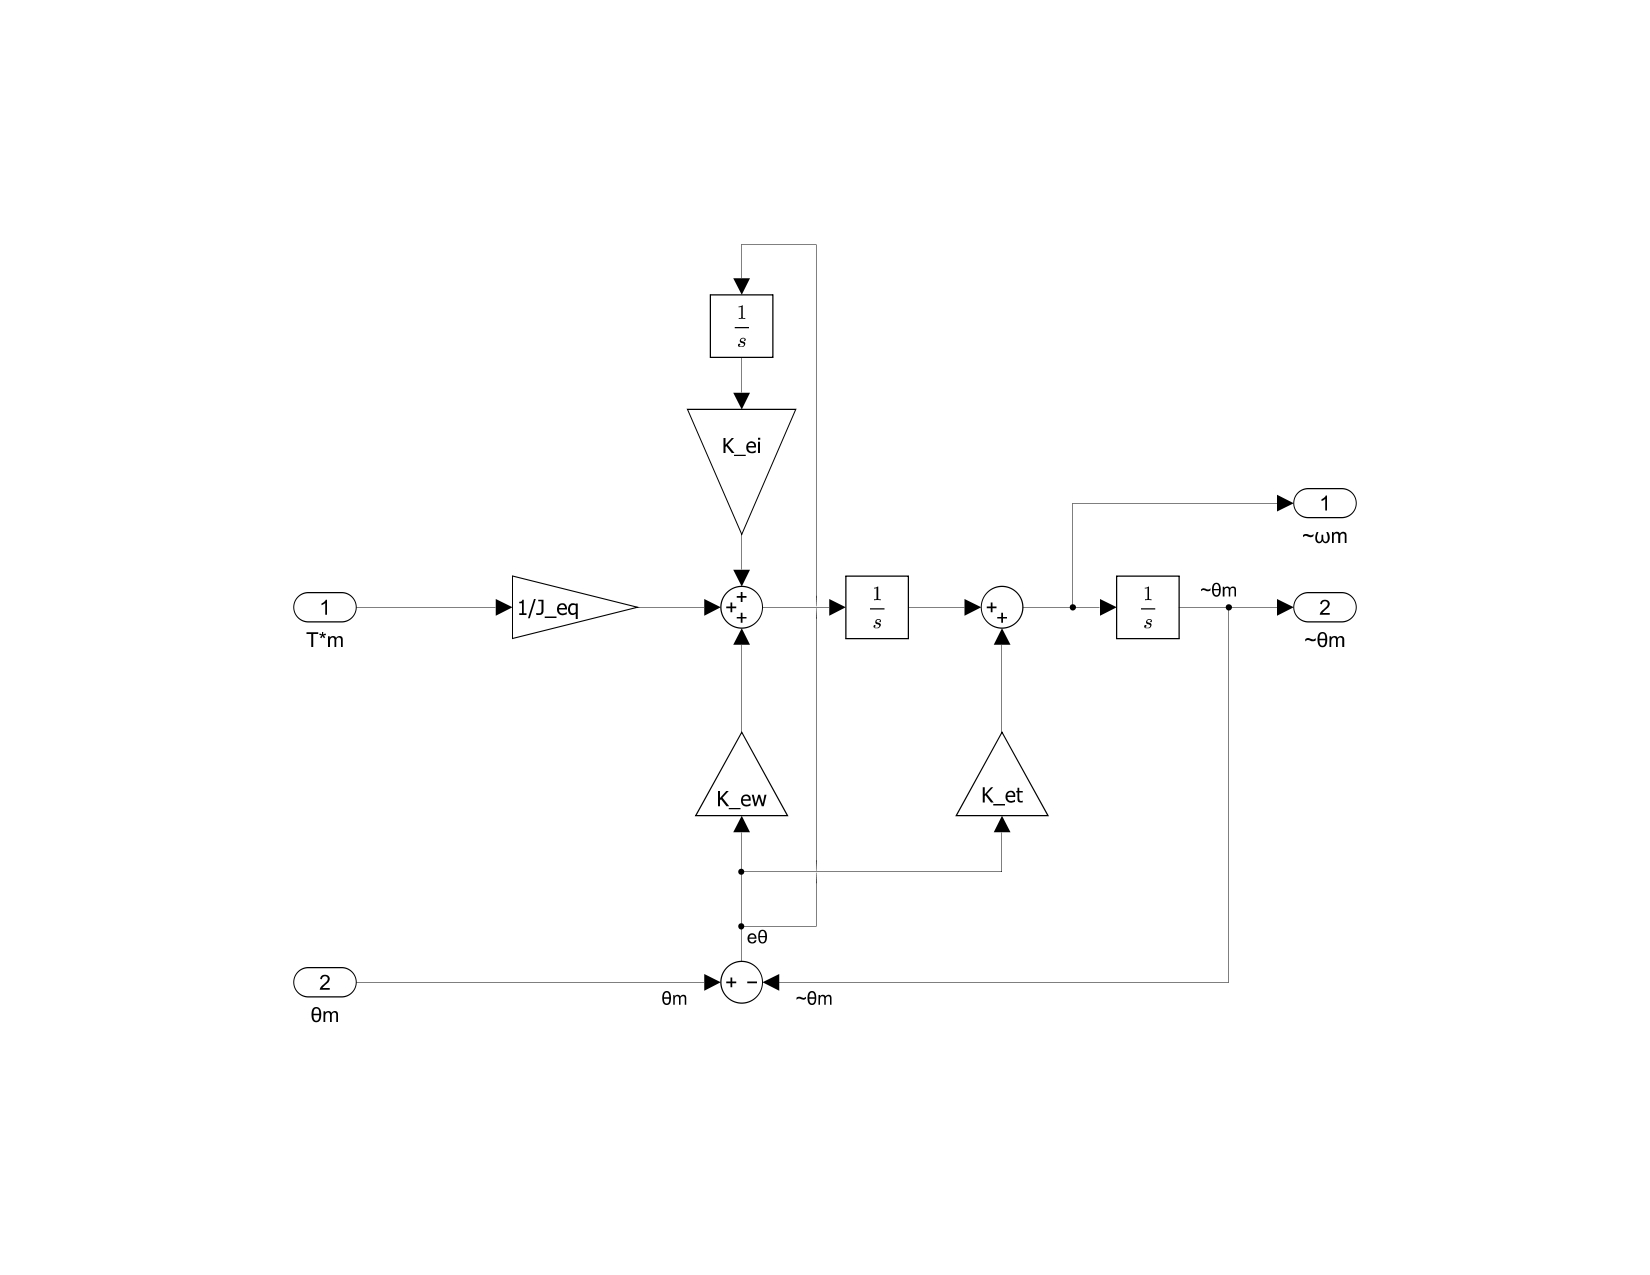
\includegraphics[width=0.74\linewidth,height=0.35\textheight,keepaspectratio]{attachments/observador_de_estado_reducido_retroalimentacion_integral.jpg}
    \captionof{figure}{Diagrama de bloques del observador con retroalimentación integral.}
    \label{fig:bloque obs de estado red con retroa integral}
\end{minipage}
\par\medskip
Simulando nuevamente el modelo con perturbación de torque $T_{ld}$ tipo escalón y consigna de posición y velocidad nulas con el observador con retroalimentación integral que se ha desarrollado, así poder evaluar si se ha conseguido el cometido de anular el error de posición angular $\theta_m$ de estado estacionario 
A continuación se ve que habiendo cambiado por el observador con retroalimentación integral el error de estado estacionario que se ha mencionado desaparece, solo queda un error transitorio en el momento de aplicación de perturbación de carga.
\begin{figure}[!htbp]
    \centering
    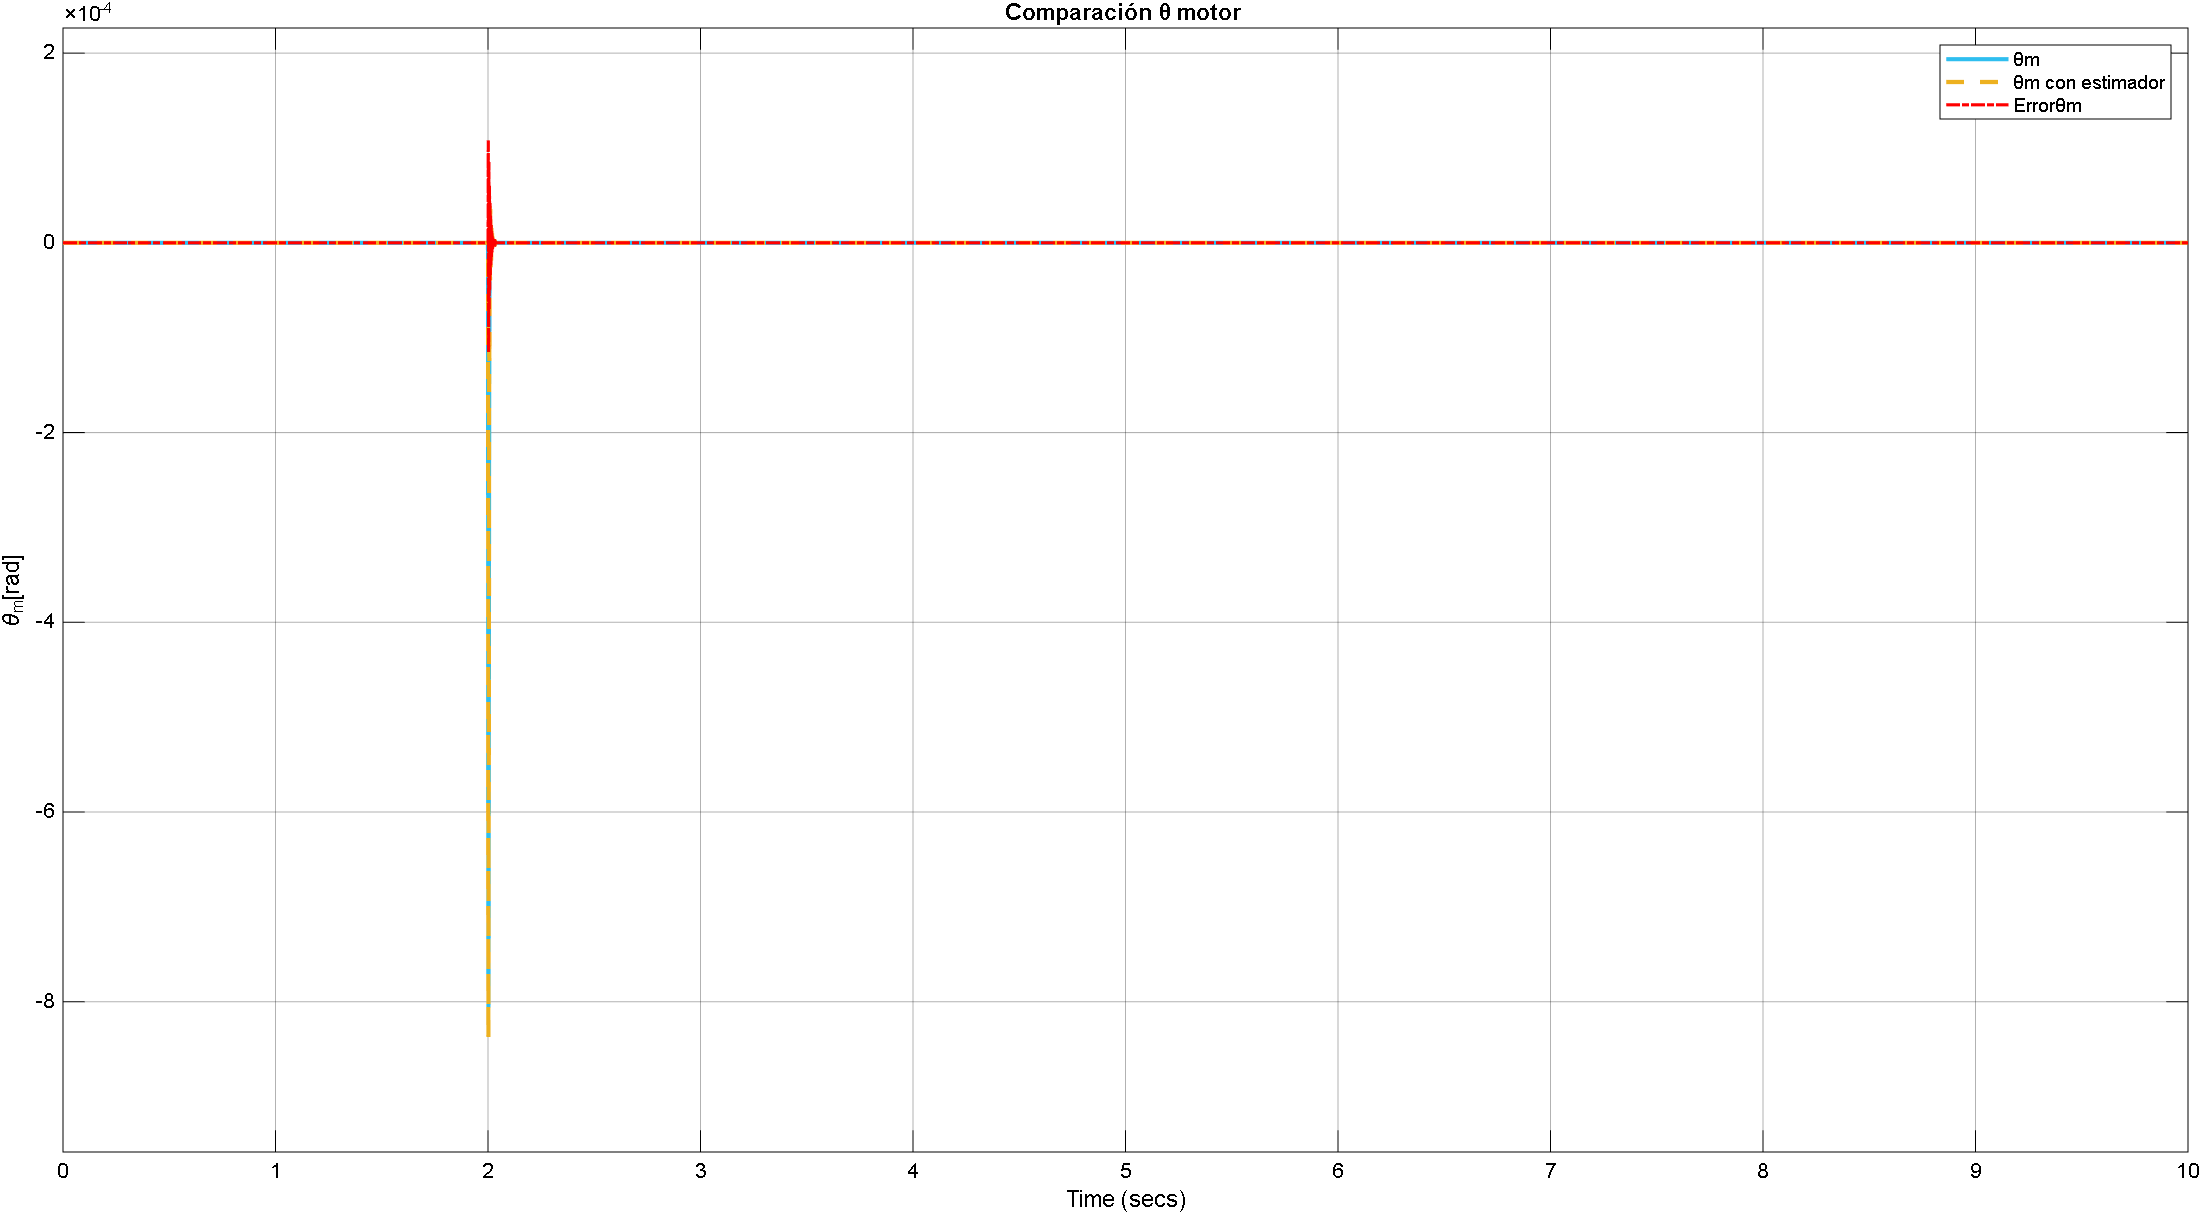
\includegraphics[width=0.86\linewidth,height=0.40\textheight,keepaspectratio]{attachments/posicion angular con perturbacion retroalimentacion integral.png}
    \caption{Comparación posición angular con y sin estimador con retroalimentación integral}
    \label{fig:posicion angular retroalimentacion integral}
    \par\medskip
    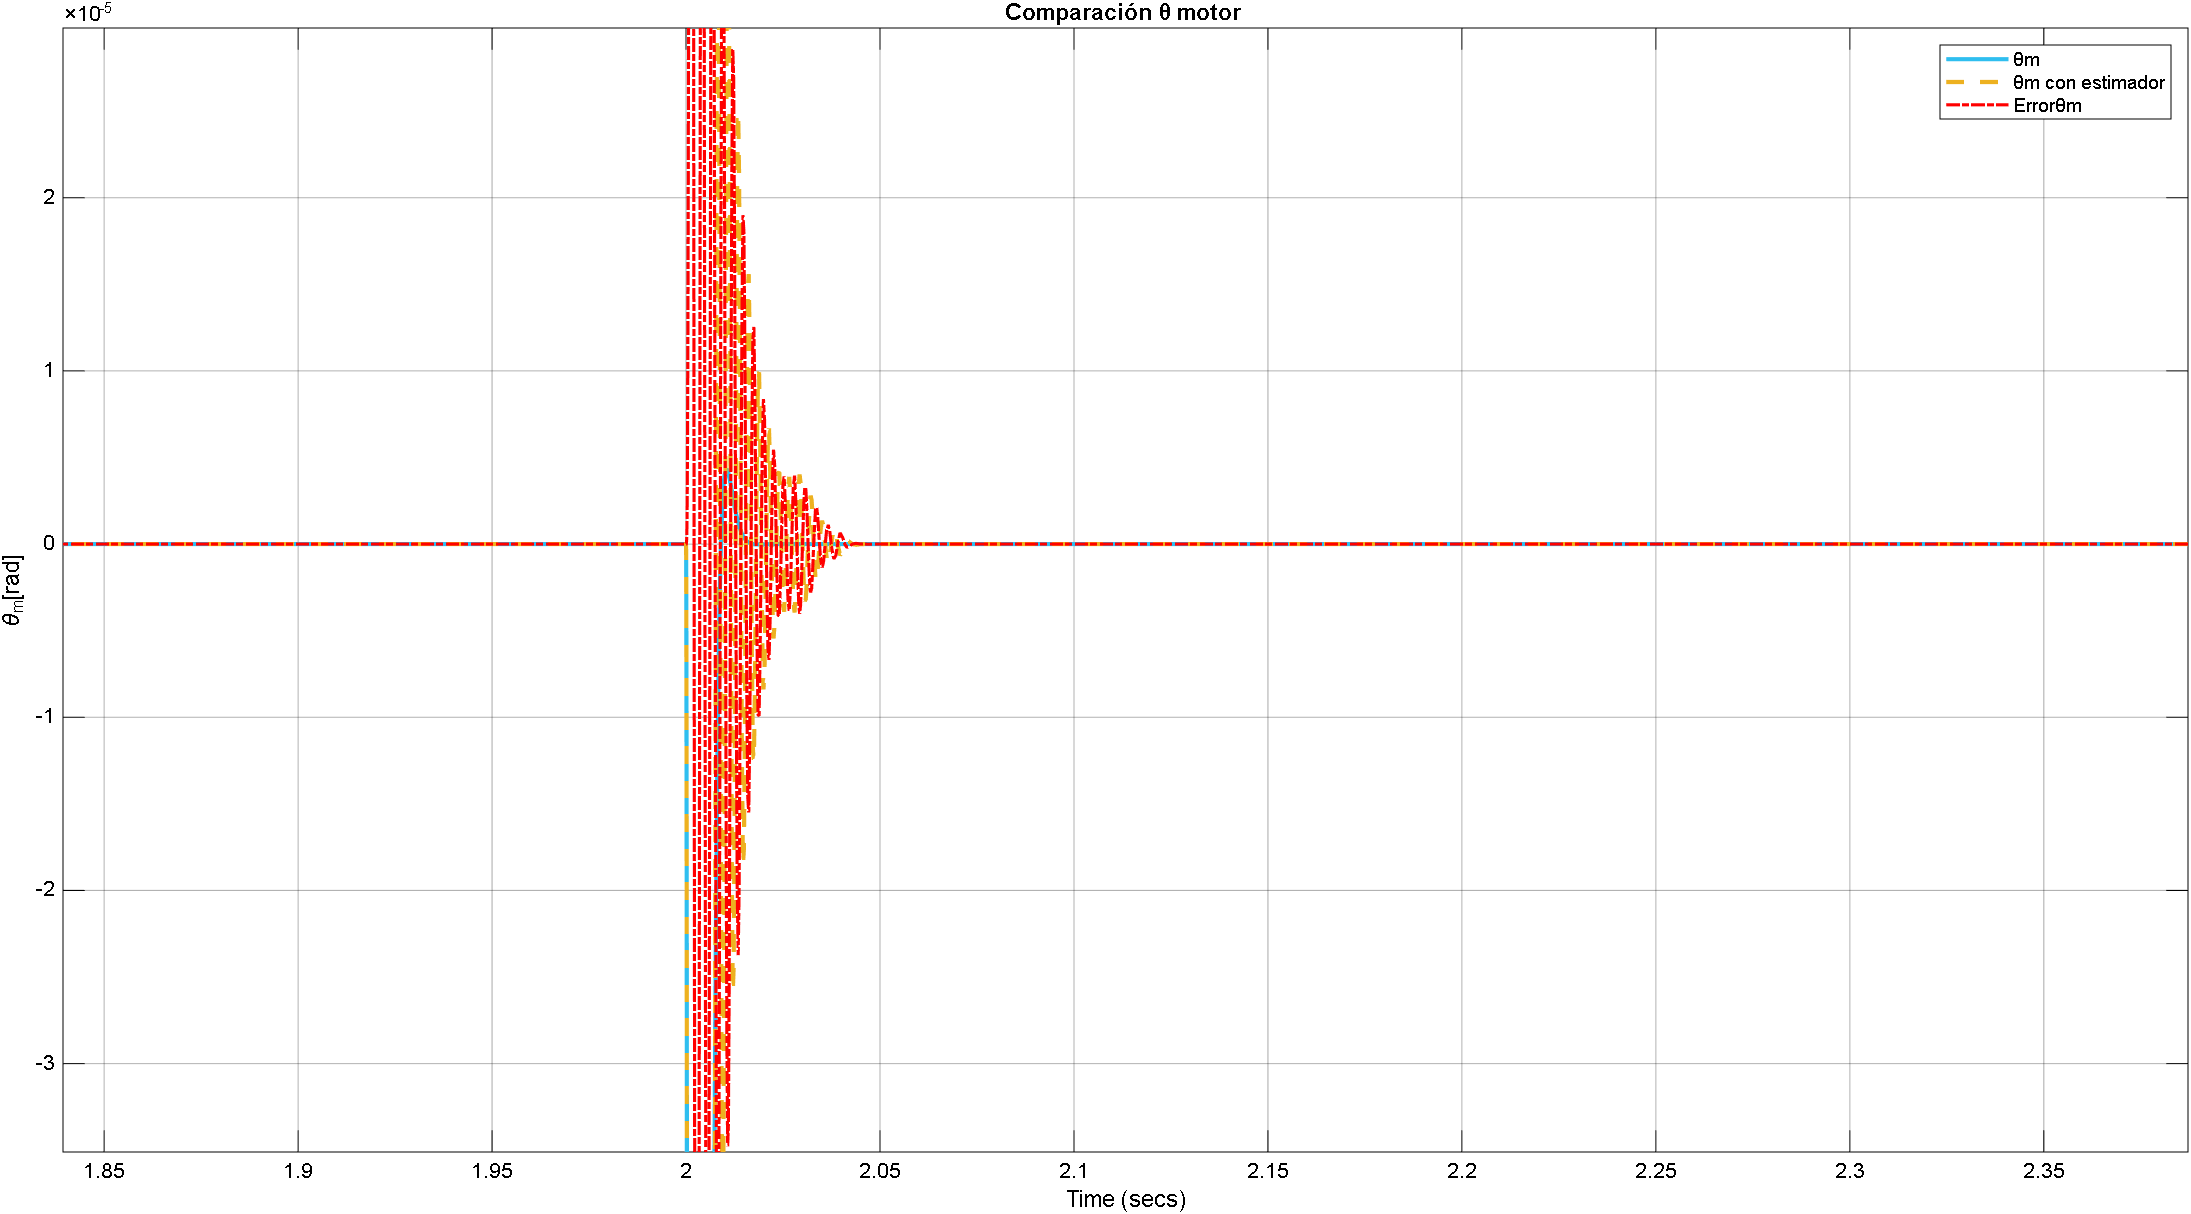
\includegraphics[width=0.86\linewidth,height=0.40\textheight,keepaspectratio]{attachments/DETALLE posicion angular con perturbacion retroalimentacion integral.png}
    \caption{DETALLE comparación posición angular con y sin estimador con retroalimentación integral}
    \label{fig:DETALLE posicion angular retroalimentacion integral}
\end{figure}
\begin{figure}[!htbp]
    \centering
    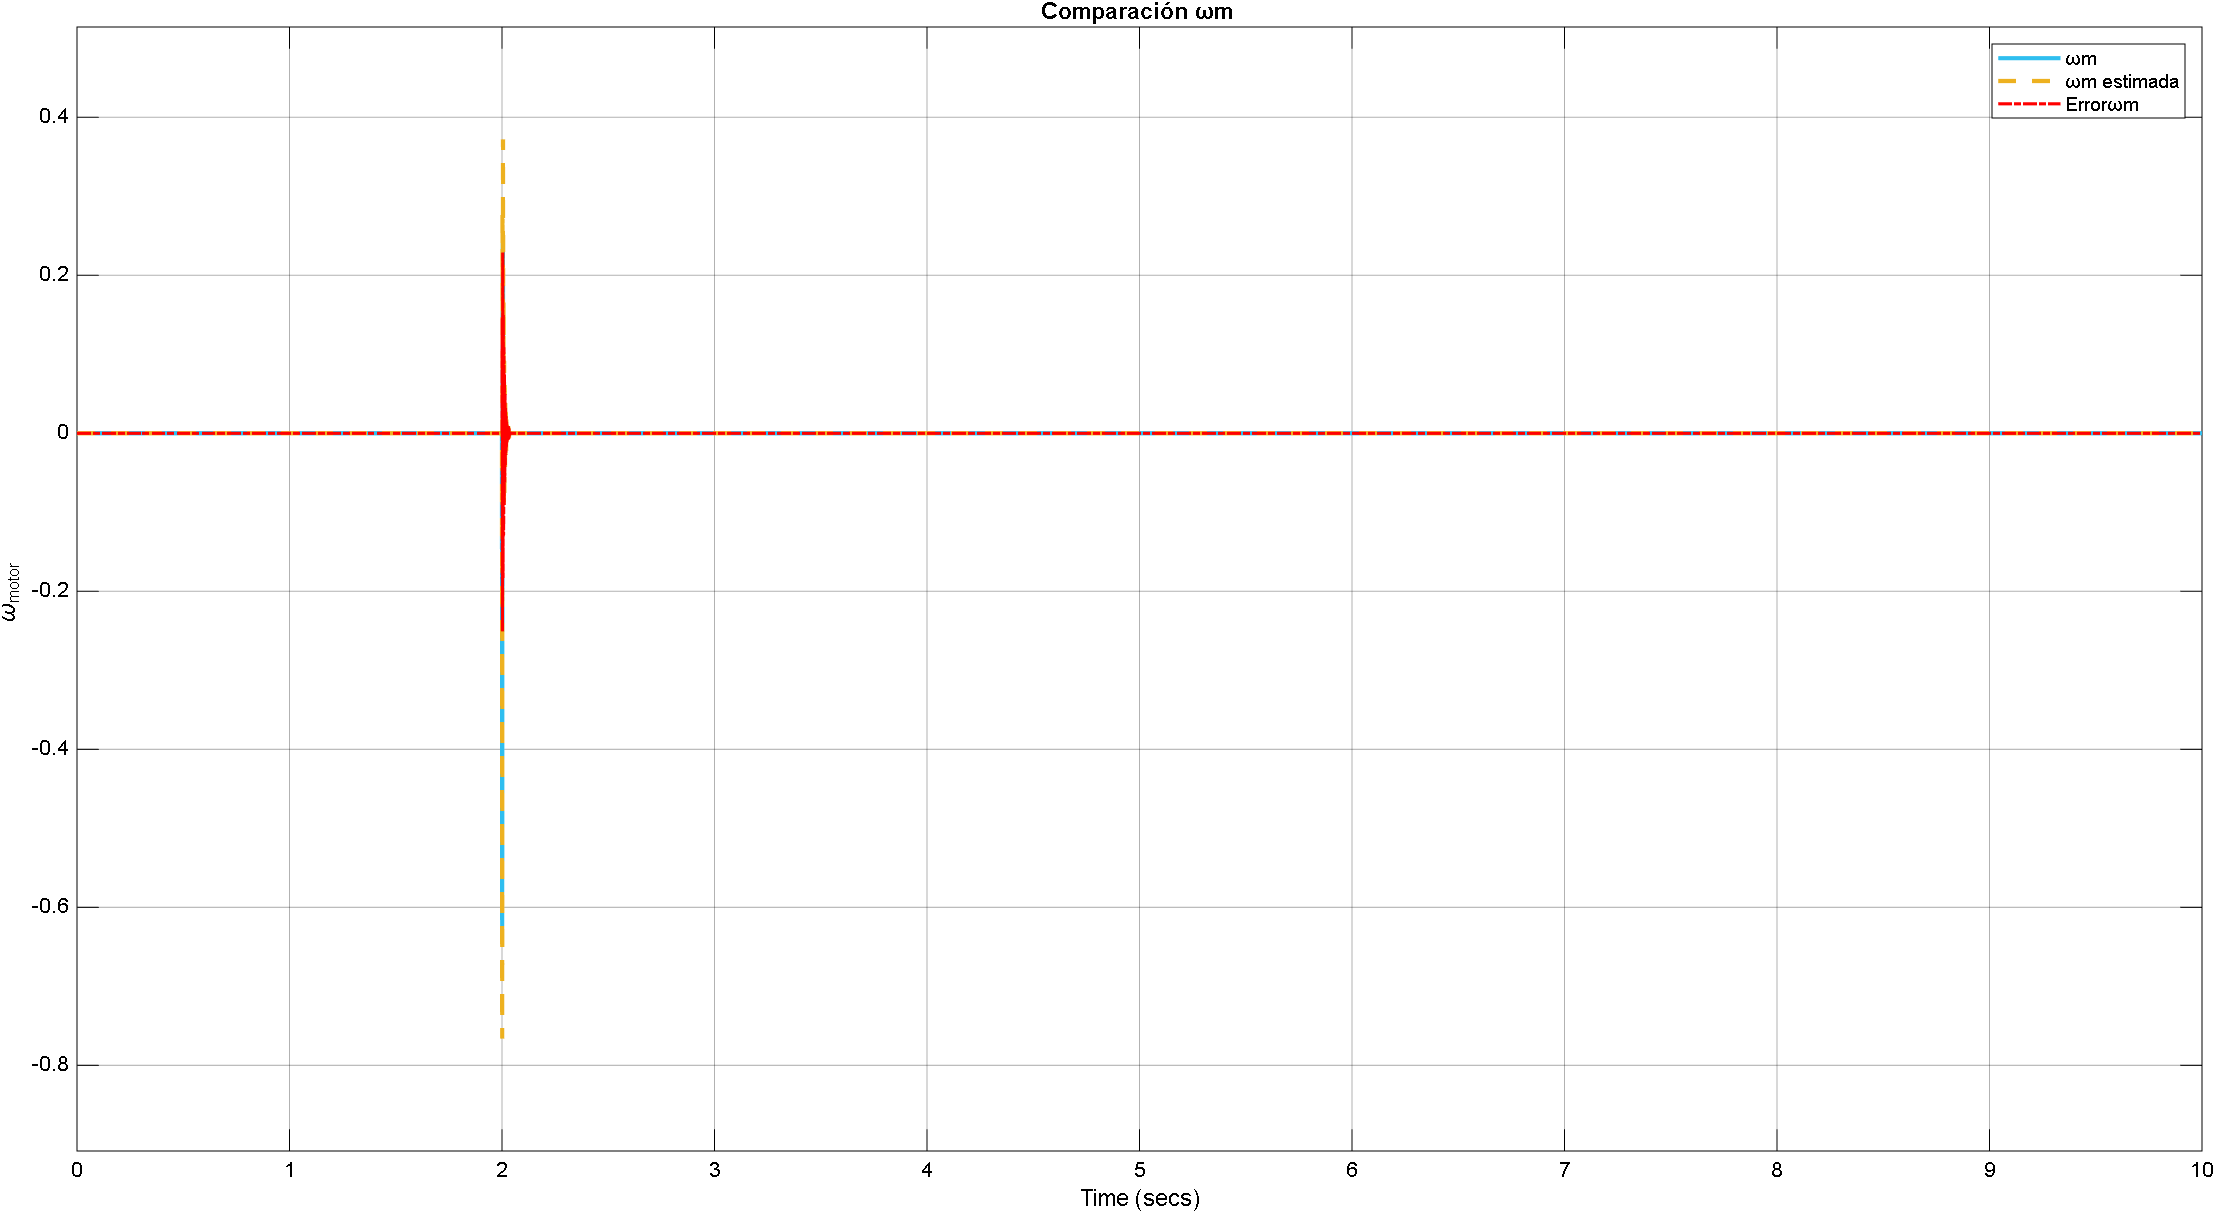
\includegraphics[width=0.86\linewidth,height=0.40\textheight,keepaspectratio]{attachments/velocidad angular con perturbacion retroalimentacion integral.png}
    \caption{Comparación velocidad angular con y sin estimador con retroalimentación integral}
    \label{fig:velocidad angular retroalimentacion integral}
    \par\medskip
    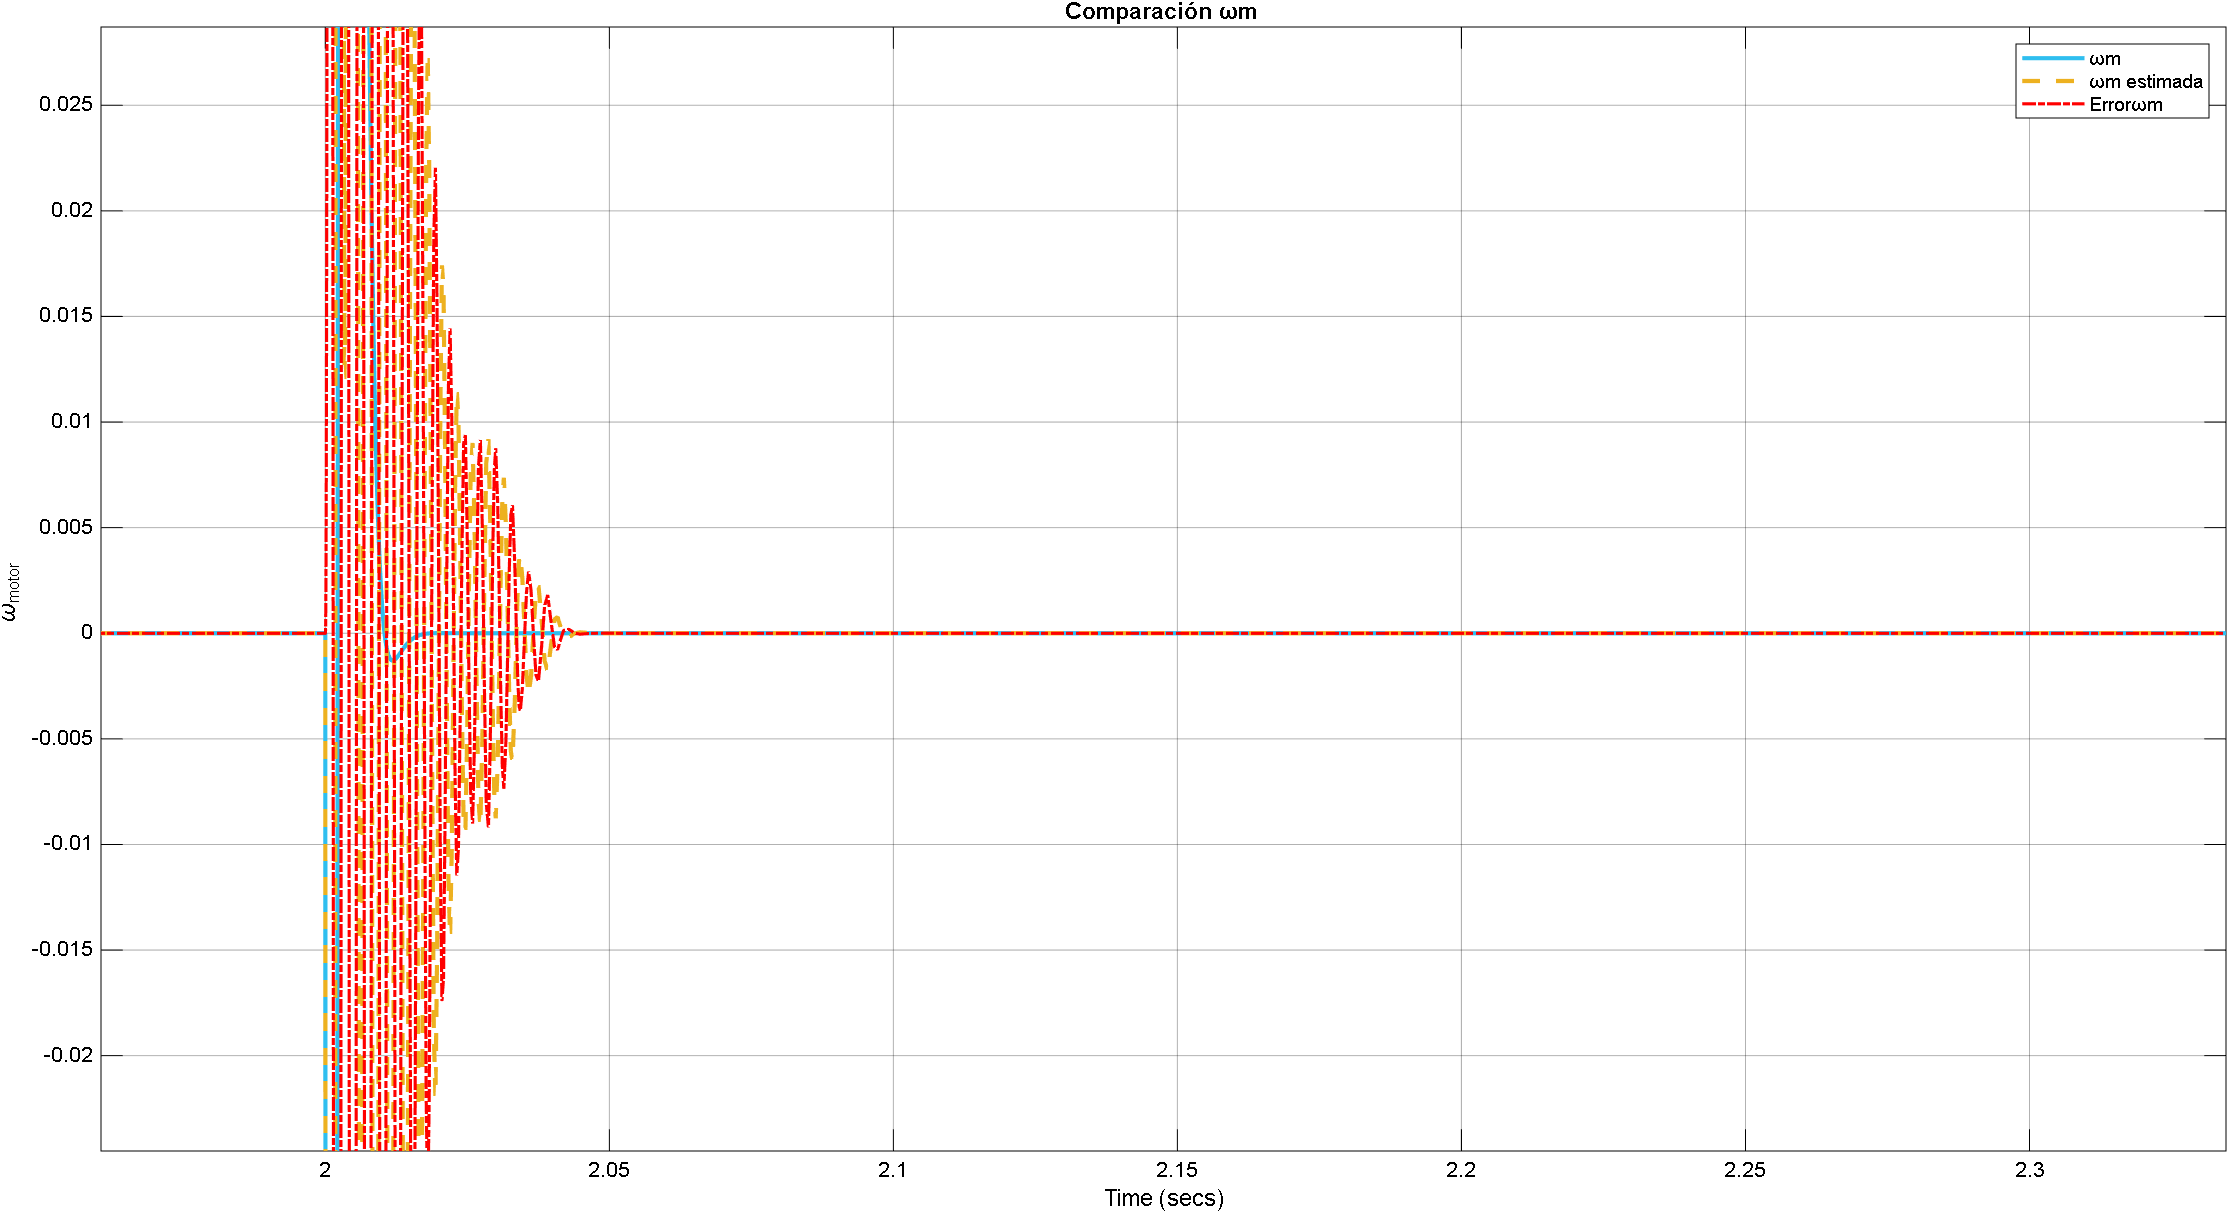
\includegraphics[width=0.86\linewidth,height=0.40\textheight,keepaspectratio]{attachments/DETALLE velocidad angular con perturbacion retroalimentacion integral.png}
    \caption{DETALLE Comparación velocidad angular con y sin estimador con retroalimentación integral}
    \label{fig:DETALLE velocidad angular retroalimentacion integral}
\end{figure}
No hubo variación en el nulo error estacionario presente en la velocidad angular $\omega_m$

\subsubsection{Comportamiento térmico}
En ésta sección se tiene la intensión de evaluar el comportamiento térmico del motor frente a exigencias de trabajo continuo. Para este cometido se plantea un escenario representativo exigente, donde: $T_{amb}=40^\circ C$ en vez de los $20^\circ$ en simulaciones anteriores, planteando la consigna suavizada de manera periódica 38 veces seguidas (tiempo de simulación $t=608\;s$), agregando además la perturbación de torque de tipo escalón planteada previamente. Se han planteado 2 escenarios que se verán a continuación:
\begin{figure}[!htbp]
    \centering
    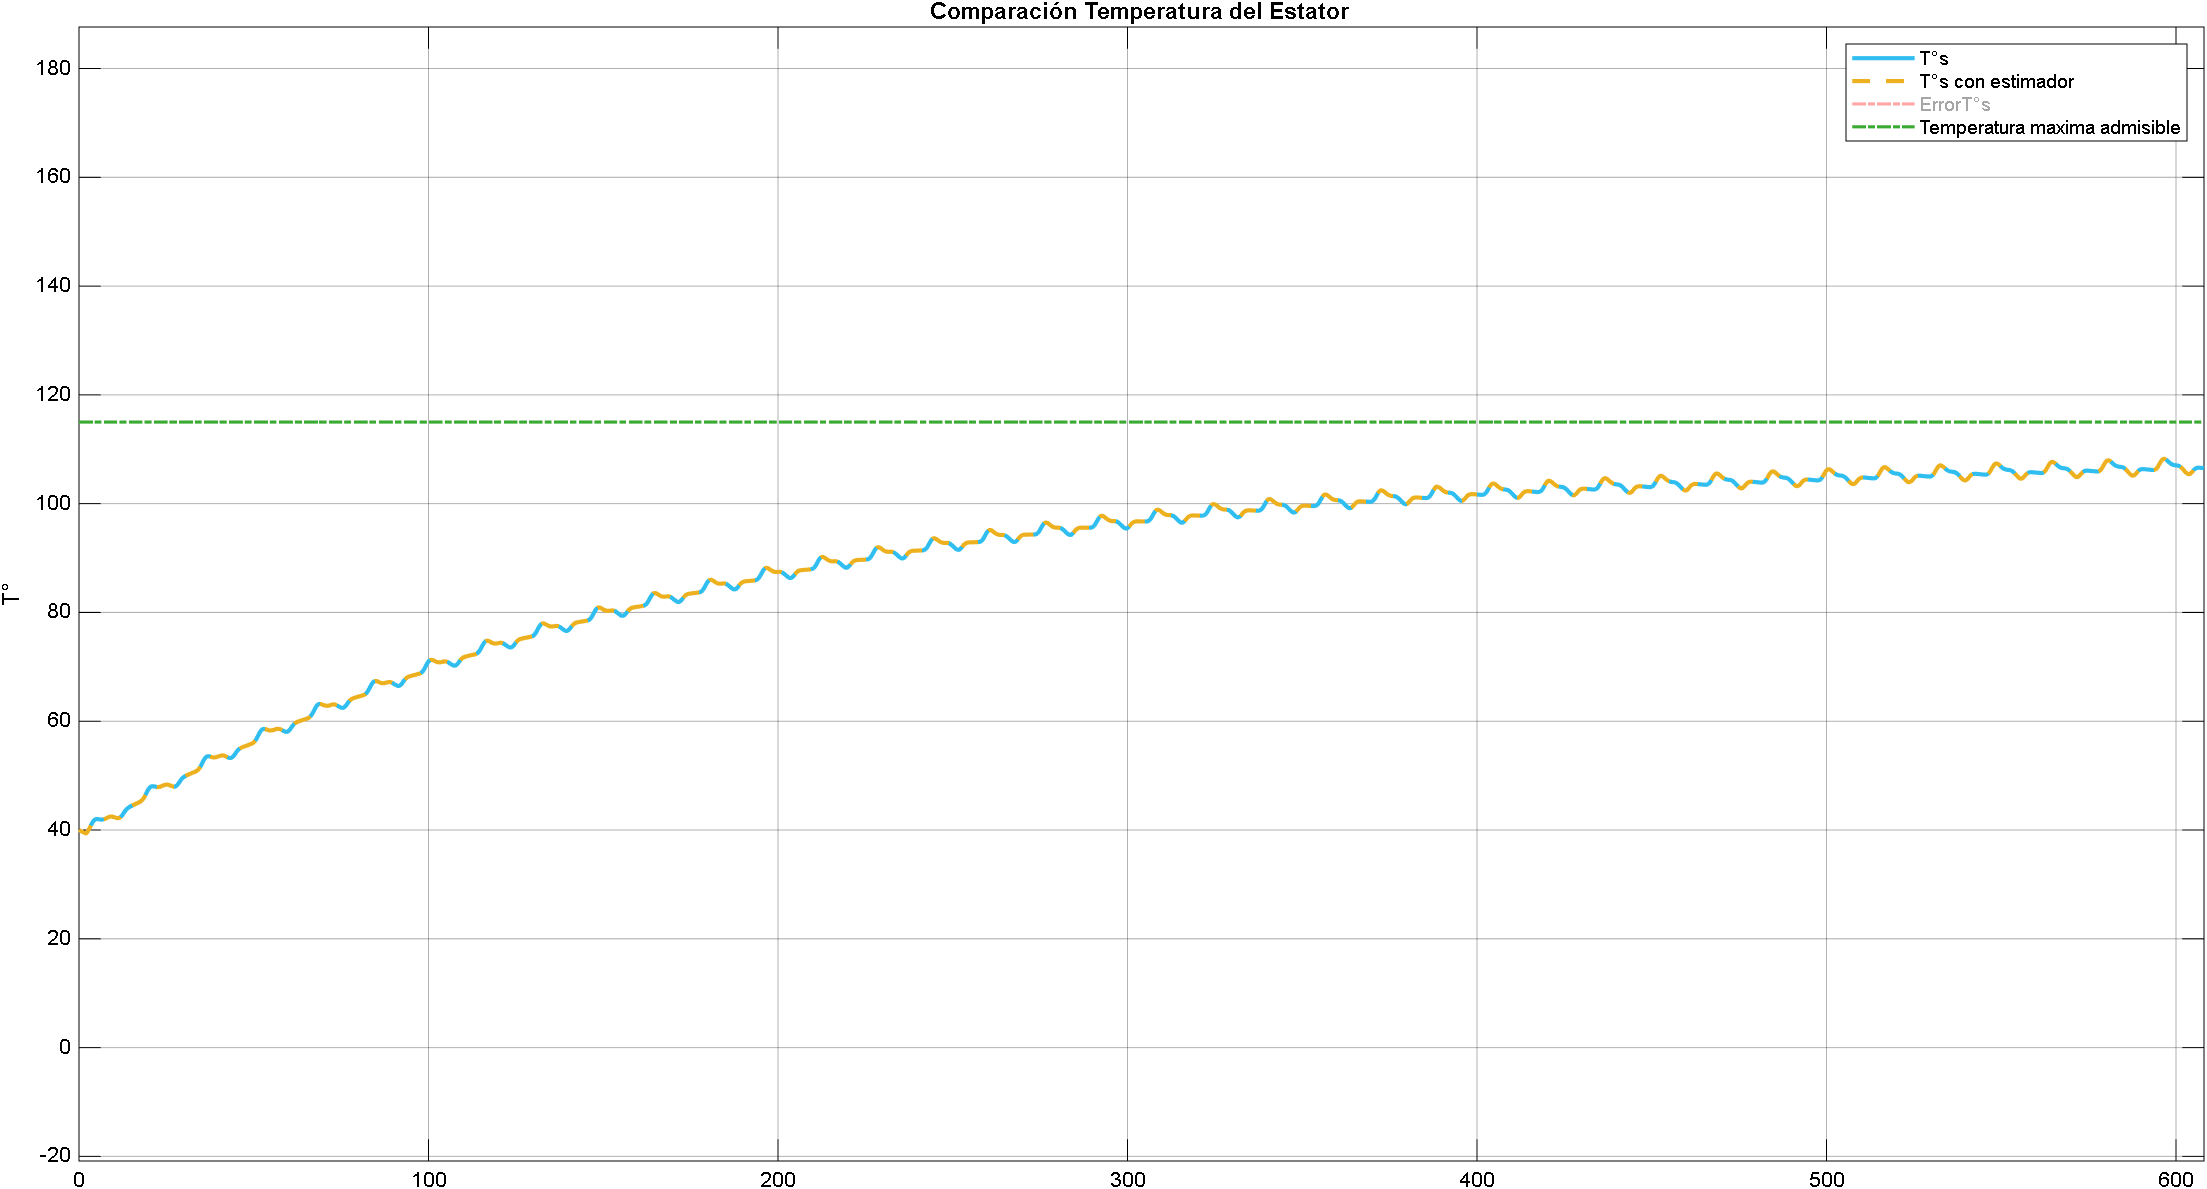
\includegraphics[width=0.78\linewidth,height=0.29\textheight,keepaspectratio]{attachments/Temperatura sin carga evaluacion.png}
    \caption{Temperatura del estator con carga nula. La línea verde marca el límite de $115\,^\circ\mathrm{C}$.}
    \label{fig:evaluacion temperatura sin carga}
    \par\medskip
    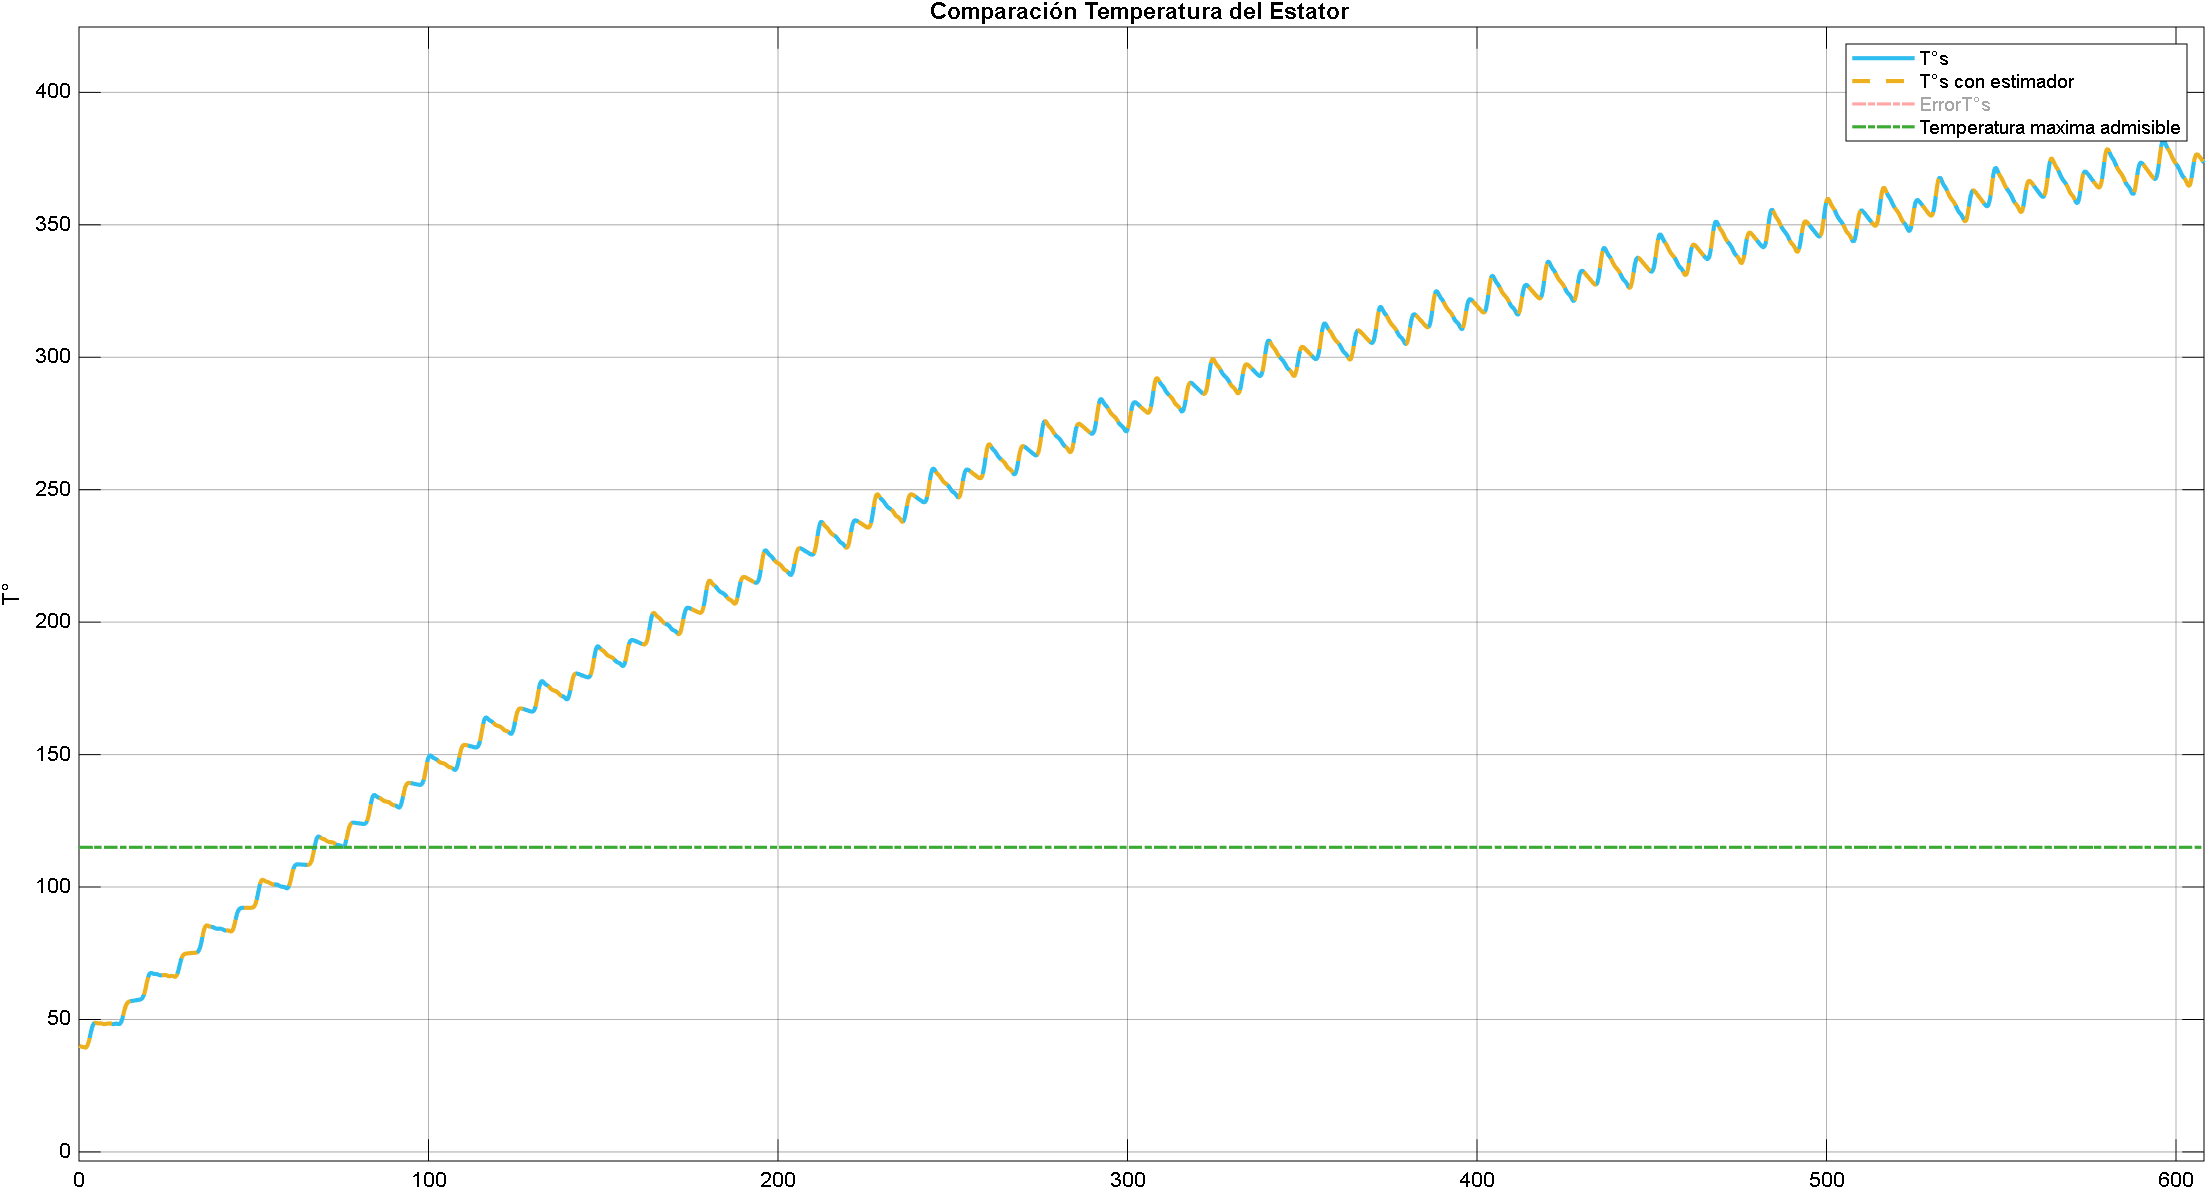
\includegraphics[width=0.78\linewidth,height=0.29\textheight,keepaspectratio]{attachments/Temperatura con carga evaluacion.png}
    \caption{Temperatura del estator con carga máxima. La línea verde marca el límite de $115\,^\circ\mathrm{C}$.}
    \label{fig:evaluacion temperatura con carga}
\end{figure}

\FloatBarrier
Con carga nula ($m_l=0\,\mathrm{kg}$), la temperatura del estator se aproxima a $108\,^\circ\mathrm{C}$ hacia el final del ensayo (Figura~\ref{fig:evaluacion temperatura sin carga}) y se mantiene por debajo del límite de $115\,^\circ\mathrm{C}$.
Con la carga máxima ($m_l=1{,}5\,\mathrm{kg}$), la temperatura del estator sigue aumentando y ronda los $375\,^\circ\mathrm{C}$ hacia el final del ensayo (Figura~\ref{fig:evaluacion temperatura con carga}), por encima del límite especificado de $115\,^\circ\mathrm{C}$. La disipación de calor por efecto Joule aumenta drásticamente debido a las elevadas corrientes en cuadratura exigidas por el lazo de control para rechazar la carga. Este sobrecalentamiento es perjudicial para la máquina, que puede provocar la degradación del material aislante del bobinado.

Finalmente se concluye que si la aplicación planteada requiere consignas de trabajo periódicas y cargas pesadas, se debe evaluar la elección de la máquina y además la posibilidad de introducir recursos adicionales de disipación térmica, tales como sistemas de refrigeración activos o ventilación forzada.
\subsubsection{Sensores no ideales}
Con la intensión de evaluar posibles degradaciones en el comportamiento dinámico global del sistema, se decide introducir la respuesta no ideal de la instrumentación debida a las limitaciones en su ancho de banda, ya que previamente se suponía sensores de ganancia unitaria y ancho de banda infinito. Para cumplir lo dicho se sustituye $G(s)\equiv1$ se sustituye por aproximaciones equivalentes, las cuales se implementan en el Espacio de Estados (SS) bajo la estructura de filtros pasa bajo (LP) de ganancia unitaria.
\paragraph{Filtro pasa bajo (LP) de segundo orden}
Este filtro tiene la siguiente función de transferencia:
\begin{equation}
    G(s) = \frac{Y(s)}{U(s)} = \frac{\omega_n^2}{s^2 + 2\xi\omega_n s + \omega_n^2}
\end{equation}
Aplicando la transformada inversa de Laplace con condiciones iniciales nulas, se obtiene la ecuación diferencial que gobierna la dinámica del sensor:
\begin{equation}
    \frac{d^2y(t)}{dt^2} + 2\xi\omega_n \frac{dy(t)}{dt} + \omega_n^2 y(t) = \omega_n^2 u(t)
\end{equation}

Definiendo el vector de estados en forma canónica controlable como $x_1(t) = y(t)$ (variable medida filtrada) y $x_2(t) = \frac{dy(t)}{dt}$ (su derivada temporal), la representación matricial en el Espacio de Estados resulta:
\begin{equation}
    \begin{bmatrix} \dot{x}_1(t) \\ \dot{x}_2(t) \end{bmatrix} = 
    \begin{bmatrix} 0 & 1 \\ -\omega_n^2 & -2\xi\omega_n \end{bmatrix} 
    \begin{bmatrix} x_1(t) \\ x_2(t) \end{bmatrix} + 
    \begin{bmatrix} 0 \\ \omega_n^2 \end{bmatrix} u(t)
\end{equation}
\begin{equation}
    y(t) = \begin{bmatrix} 1 & 0 \end{bmatrix} \begin{bmatrix} x_1(t) \\ x_2(t) \end{bmatrix}
\end{equation}
De acuerdo con las especificaciones dadas, los parámetros nominales ($\times 1$) son:
\begin{itemize}
    \item \textbf{Sensores de corriente ($i_{as}, i_{bs}, i_{cs}$):} filtro LP de 2.º orden críticamente amortiguado con $\omega_{n,i} = 6000\text{ rad/s}$ y $\xi = 1$ ($\omega_{n,i}^2 = 3,6 \times 10^7\text{ rad}^2/\text{s}^2$, $2\xi\omega_{n,i} = 12000\text{ rad/s}$).
    \item \textbf{Sensor de posición angular ($\theta_m$):} filtro LP de 2.º orden críticamente amortiguado con $\omega_{n,\theta} = 2000\text{ rad/s}$ y $\xi = 1$ ($\omega_{n,\theta}^2 = 4 \times 10^6\text{ rad}^2/\text{s}^2$, $2\xi\omega_{n,\theta} = 4000\text{ rad/s}$).
    \item \textbf{Condiciones iniciales externas:} Dado que el accionamiento inicia desde el reposo ($\theta_m(0) = 0\text{ rad}$, $i_{abcs}(0) = 0\text{ A}$), ambos integradores de cada filtro se inicializan mediante condición inicial externa en cero ($x_1(0) = u(0) = 0$ y $x_2(0) = 0$).
\end{itemize}
Con lo anterior se obtienen los sensores de corriente y posición.
\FloatBarrier
\begin{figure}[htpb]
    \centering
    \includegraphics[width=1\linewidth]{sensor_real_corriente.jpg}
    \caption{Bloque de implementación Sensor no lineal de corriente}
    \label{fig:sensor no lineal corriente}
\end{figure}
\FloatBarrier
\begin{figure}[htpb]
    \centering
    \includegraphics[width=1\linewidth]{sensor_real_posicion.jpg}
    \caption{Bloque de implementación Sensor no lineal de posición angular}
    \label{fig:sensor no lineal posición}
\end{figure}
\FloatBarrier
\paragraph{Filtro pasa bajo (LP) de primer orden}
El sensor térmico se modela como un filtro pasa bajos de primer orden de ganancia unitaria:
\begin{equation}
    G_T(s) = \frac{Y(s)}{U(s)} = \frac{1}{\tau s + 1}
\end{equation}

En el dominio del tiempo, la ecuación diferencial asociada es $\tau \frac{dy(t)}{dt} + y(t) = u(t)$.
Con la constante de tiempo especificada $\tau = 20\;s$ ($1/\tau = 0,05\;s^{-1}$), y siguiendo la recomendación de calibración inicial para evitar transitorios ficticios de medición, se asigna al integrador una condición inicial externa igual a la temperatura inicial del bobinado ($ T^\circ_s(0) = T^\circ_{amb}=20^\circ C$).
\paragraph{Conclusiones de simulaciones con ($\omega _n \times1$)}


Al incorporar los filtros pasa bajos con las frecuencias naturales nominales ($\omega_{n,\theta} = 2000\text{rad/s}$, $\omega_{n,i} = 6000\text{rad/s}$ y $\tau = 20\text{s}$) sobre el sistema completo con observador de estado con acción integral y consigna de velocidad suavizada, se observa una severa degradación del desempeño que conduce a la inestabilidad del lazo cerrado:
\begin{enumerate}
    \item \textbf{Advertencia del solver y divergencia en $t \approx 1,142\text{ s}$:} Al iniciarse el perfil de movimiento en $t = 1\text{ s}$, el retraso dinámico introducido por los sensores provoca que en $t = 1,142\text{ s}$ el sistema entre en oscilación divergente. El solver de paso variable de Simulink reduce su paso de integración hasta alcanzar el límite mínimo permitido ($4,057 \times 10^{-15}\text{ s}$), emitiendo una advertencia por rigidez numérica (\textit{stiffness}).
    \item \textbf{Interacción con la Transformación de Park y el Observador:} El filtro de posición ($\omega_{n,\theta} = 2000\text{ rad/s}$) introduce un retardo de $t_{d,\theta} \approx \frac{2\xi}{\omega_n} = 1\text{ ms}$, ubicando sus polos por debajo de los del observador ($p_{obs} = -3200\text{ rad/s}$). Durante la aceleración, este desfasaje en el ángulo eléctrico $\theta_{r,\text{med}}$ desalinea los ejes $dq0$ en las transformaciones de Park (generando acoplamientos cruzados) y hace que el integrador del observador acumule el error de retraso hasta saturar el lazo.
    \item \textbf{Pérdida de margen de fase en los lazos de corriente:} Los polos del sensor de corriente ($\omega_{n,i} = 6000\text{ rad/s}$, $t_{d,i} \approx 0,33\text{ ms}$) quedan muy próximos a los polos de diseño del lazo cerrado de corriente ($p_i = -5000\text{ rad/s}$), reduciendo el margen de fase y degradando la estabilidad.
    \item \textbf{Divergencia de las variables simuladas ($\omega_n \times 1$):} En $t = 1,142\text{ s}$ se producen picos transitorios no físicos en corrientes ($\sim 600\text{ A}$), tensiones ($10^{16}$--$10^{17}\text{ V}$) y torque ($-2 \times 10^8\text{ N}\cdot\text{m}$). Por efecto de los integradores del sistema, este impulso provoca que la posición estimada $\hat{\theta}_m(t)$ diverja linealmente ($-3,2 \times 10^5\text{ rad}$) y que la temperatura estimada $T^\circ_s(t)$ crezca cuadráticamente ($10^{12}\text{ }^\circ\text{C}$).
\end{enumerate}
\FloatBarrier
\begin{figure}
    \centering
    \includegraphics[width=1\linewidth]{posicion con sensor real x1.png}
    \caption{Posición Angular con y sin estimación con sensores no ideales}
    \label{fig:posicion angular sensor no ideal}

\end{figure}
\FloatBarrier
\begin{figure}
    \centering
    \includegraphics[width=1\linewidth]{velocidad con sensor real x1.png}
    \caption{Velocidad Angular con y sin estimación con sensores no ideales}
    \label{fig:velocidad angular sensor no ideal}
\end{figure}
\FloatBarrier
\begin{figure}
    \centering
    \includegraphics[width=1\linewidth]{temperatura con sensor real x1.png}
    \caption{Torque motor con y sin estimación con sensores no ideales}
    \label{fig:torque motor sensor real}
\end{figure}
\FloatBarrier
\begin{figure}
    \centering
    \includegraphics[width=1\linewidth]{Idq0 con sensor real x1.png}
    \caption{Corrientes virtuales $i_{dq0}$ con y sin estimación con sensores no ideales}
    \label{fig:corrientes virtuales sensor real}
\end{figure}
\FloatBarrier
\begin{figure}
    \centering
    \includegraphics[width=1\linewidth]{Iabc con sensor real x1.png}
    \caption{Corrientes reales $i_{abc}$ con y sin estimación con sensores no ideales}
    \label{fig:corrientes reales sensor real}
\end{figure}
\FloatBarrier
\paragraph{Conclusiones de simulaciones con ($\omega _n \times2$  )}
Se evalúa el efecto de incrementar las frecuencias naturales de los sensores de posición y corriente.
\begin{itemize}
    \item \textbf{Recuperación de la estabilidad con $\omega_n \times 2$:} Al duplicar las frecuencias naturales ($\omega_{n,\theta} = 4000\text{ rad/s}$ y $\omega_{n,i} = 12000\text{ rad/s}$), los polos de los sensores se desplazan hacia altas frecuencias por encima de los polos dominantes del observador ($-3200\text{ rad/s}$) y del lazo de corriente ($-5000\text{ rad/s}$). En consecuencia, desaparecen los impulsos numéricos, las curvas de posición ($\theta_m$), velocidad ($\omega_m$) y torque ($T_m$) estimadas se superponen perfectamente con las reales, y los errores de estimación convergen a cero.
    
    \item \textbf{Influencia del sensor de temperatura ($\tau = 20\text{ s}$):} Debido a que la constante de tiempo térmica propia del estator ($\tau_{ts-amb} = R_{ts-amb} \cdot C_{ts} \approx 120\text{ s}$) es un orden de magnitud superior a la del sensor ($\tau = 20\text{ s}$), este filtro no compromete la estabilidad del lazo electromecánico ni el seguimiento de trayectoria, introduciendo únicamente un leve desfasaje durante los transitorios térmicos lentos en la actualización de $R_s(T^\circ_s)$.
\end{itemize}
\FloatBarrier
\begin{figure}
    \centering
    \includegraphics[width=1\linewidth]{posicion con sensor real x2.png}
    \caption{Posición Angular con y sin estimación con sensores no ideales con ancho de banda aumentado $\times2$}
    \label{fig:posicion angular sensor no ideal x2}
\end{figure}
\FloatBarrier
\begin{figure}
    \centering
    \includegraphics[width=1\linewidth]{velocidad con sensor real x2.png}
    \caption{Velocidad Angular con y sin estimación con sensores no ideales con ancho de banda aumentado $\times2$}
    \label{fig:velocidad angular sensor no ideal x2}
\end{figure}
\FloatBarrier
\begin{figure}
    \centering
    \includegraphics[width=1\linewidth]{torque con sensor real x2.png}
    \caption{Torque motor con y sin estimación con sensores no ideales con ancho de banda aumentado $\times2$}
    \label{fig:torque motor sensor no ideal x2}
\end{figure}
\FloatBarrier
\begin{figure}
    \centering
    \includegraphics[width=1\linewidth]{temperatura con sensor real x2.png}
    \caption{Temperatura del estator con y sin estimación con sensores no ideales con ancho de banda aumentado $\times2$}
    \label{fig:temperatura del estator sensor no ideal x2}
\end{figure}
\FloatBarrier
\begin{figure}
    \centering
    \includegraphics[width=1\linewidth]{Idq0 con sensor real x2.png}
    \caption{Corrientes virtuales $i_{dq0}$ con y sin estimación con sensores no ideales con ancho de banda aumentado $\times2$}
    \label{fig:Idq0 sensor no ideal x2}
\end{figure}
\FloatBarrier
\begin{figure}
    \centering
    \includegraphics[width=1\linewidth]{Iabc con sensor real x2.png}
    \caption{Corrientes reales $i_{abc}$ con y sin estimación con sensores no ideales con ancho de banda aumentado $\times2$}
    \label{fig:Iabc sensor no ideal x2}
\end{figure}
\FloatBarrier
\subsubsection{Modulador de tensión trifásico no ideal}
Con el fin de evaluar la degradación del desempeño del sistema ante las limitaciones físicas de la etapa de potencia, se reemplaza el inversor ideal asumido inicialmente ($G(s) \equiv 1$) por un modelo aproximado equivalente que contempla tanto el ancho de banda limitado como la saturación de tensión del puente trifásico.
La dinámica de cada fase del modulador ($v_{as}, v_{bs}, v_{cs}$) se modela mediante un filtro pasa bajos de segundo orden con ganancia unitaria y amortiguamiento crítico ($\xi = 1$).
\begin{equation}
    G_{mt}(s) = \frac{Y(s)}{U(s)} = \frac{\omega_n^2}{s^2 + 2\xi\omega_n s + \omega_n^2}
\end{equation}
Definiendo el vector de estados en forma canónica controlable como $x_1(t) = y(t)$ y $x_2(t) = \frac{dy(t)}{dt}$, la representación matricial en el Espacio de Estados resulta:
\begin{equation}
    \begin{bmatrix} \dot{x}_1(t) \\ \dot{x}_2(t) \end{bmatrix} = 
    \begin{bmatrix} 0 & 1 \\ -\omega_n^2 & -2\xi\omega_n \end{bmatrix} 
    \begin{bmatrix} x_1(t) \\ x_2(t) \end{bmatrix} + 
    \begin{bmatrix} 0 \\ \omega_n^2 \end{bmatrix} u(t), \qquad
    y(t) = \begin{bmatrix} 1 & 0 \end{bmatrix} \begin{bmatrix} x_1(t) \\ x_2(t) \end{bmatrix}
\end{equation}
con condiciones iniciales externas nulas ($x_1(0) = x_2(0) = 0$).
A la salida de cada filtro se incorpora un bloque de saturación simétrica que limita la amplitud instantánea de la tensión de fase en bornes del estator según el límite máximo del bus de continua ($V_{sl\text{-max}} = 48\text{ V}_{ca\text{-rms}}$):
\begin{equation}
    |y(t)| \le \frac{\sqrt{2} \cdot V_{sl\text{-max}}}{\sqrt{3}} \approx 39,192\text{ V}
\end{equation}
\FloatBarrier
\begin{figure}
    \centering
    \includegraphics[width=1\linewidth]{Inversor_Real_unidad.jpg}
    \caption{Inversor real con ganancia unitaria subbloque para una sola fase}
    \label{fig:Inversor real unidad}
\end{figure}
\FloatBarrier
\begin{figure}
    \centering
    \includegraphics[width=1\linewidth]{Inversor_Real_completo.jpg}
    \caption{Inversor real trifásico con ganancia unitaria y saturación}
    \label{fig:Inversor real Completo}
\end{figure}
\FloatBarrier

\paragraph{Conclusiones de simulaciones }


Se evalúa el comportamiento del accionamiento frente a la consigna trapezoidal de movimiento al variar la frecuencia natural del modulador manteniendo $\xi = 1$ y la saturación en $\pm 39,192\text{ V}$
\paragraph{Simulación con $\omega_n \times 1$}
\FloatBarrier
\begin{figure}[htpb]
    \centering
    \includegraphics[width=1\linewidth]{posicion con inversor real x1.png}
    \caption{Posición Angular comparación con y sin estimación, con sensores no lineales e inverter no lineal}
    \label{fig:inverter real posicion x1}
\end{figure}
\FloatBarrier
\begin{figure}[htpb]
    \centering
    \includegraphics[width=1\linewidth]{velocidad con inversor real x1.png}
    \caption{Velocidad Angular comparación con y sin estimación, con sensores no lineales e inverter no lineal con $\omega_n \times1$}
    \label{fig:inverter real velocidad x1}
\end{figure}
\FloatBarrier
Es posible observar que el sistema presenta una severa degradación e inestabilidad en el seguimiento tanto en posición angular como en velocidad angular. Esta situación se traduce en transitorios abruptos y quiebres severos en la respuesta temporal, evidenciando que las restricciones dinámicas de la etapa de modulación penalizan fuertemente el desempeño global del lazo cerrado.

\paragraph{Simulación con $\omega_n \times 2$}
\begin{figure}[htpb]
    \centering
    \includegraphics[width=1\linewidth]{posicion con inversor real x2.png}
    \caption{Posición Angular comparación con y sin estimación, con sensores no lineales e inverter no lineal con $\omega_n \times2$}
    \label{fig:inverter real posicion x2}
\end{figure}
\FloatBarrier
\begin{figure}[htpb]
    \centering
    \includegraphics[width=1\linewidth]{velocidad con inversor real x2.png}
    \caption{Velocidad Angular comparación con y sin estimación, con sensores no lineales e inverter no lineal con $\omega_n \times2$}
    \label{fig:inverter real velocidad x2}
\end{figure}
\FloatBarrier
Al doblar las frecuencias de lo visto previamente, es posible concluir que el sistema presenta una notable mejoría en el seguimiento de la consigna de posición, esto se debe a la reducción del retado propio a la etapa de modulación. 
% ---------------------------------------------------------------------------- %
\subsection{Versión final y discretización}

El modelo de la aplicación se organiza en cuatro grupos funcionales:


\begin{itemize}
    \item \textbf{Controlador:} comprende los algoritmos que calculan las acciones de control a partir de las referencias y de las variables medidas o estimadas, con el objetivo de satisfacer la consigna de movimiento.

    \item \textbf{Actuador:} representa el dispositivo físico encargado de aplicar a la planta las acciones solicitadas por el controlador. En esta aplicación corresponde al inversor trifásico, cuya dinámica se aproxima mediante un filtro pasabajos de segundo orden, con factor de amortiguamiento $\zeta=1$ y frecuencia natural $\omega_n=6000\;\mathrm{rad/s}$.

    \item \textbf{Planta:} representa el sistema físico que se desea controlar e incluye la máquina PMSM, el tren de transmisión y la carga, junto con sus dinámicas electromagnéticas, mecánicas y térmicas. La validez de los resultados de simulación depende de la fidelidad de este modelo y de las hipótesis adoptadas. Por ello, el desempeño obtenido en simulación debe evaluarse considerando las incertidumbres, las perturbaciones y las limitaciones de los componentes antes de extrapolarlo al sistema real.

    \item \textbf{Sensores:} proporcionan las mediciones utilizadas por el controlador. Su comportamiento depende del rango de medida, el ancho de banda, el sesgo, el ruido y la resolución, entre otras características. Estas limitaciones pueden introducir diferencias entre las variables físicas de la planta y las señales disponibles para la realimentación.
\end{itemize}

La Figura~\ref{fig:sistema-final-continuo} presenta la estructura integrada del sistema de control en tiempo continuo, utilizada como referencia para desarrollar la implementación digital.

\begin{figure}[!htbp]
    \centering
    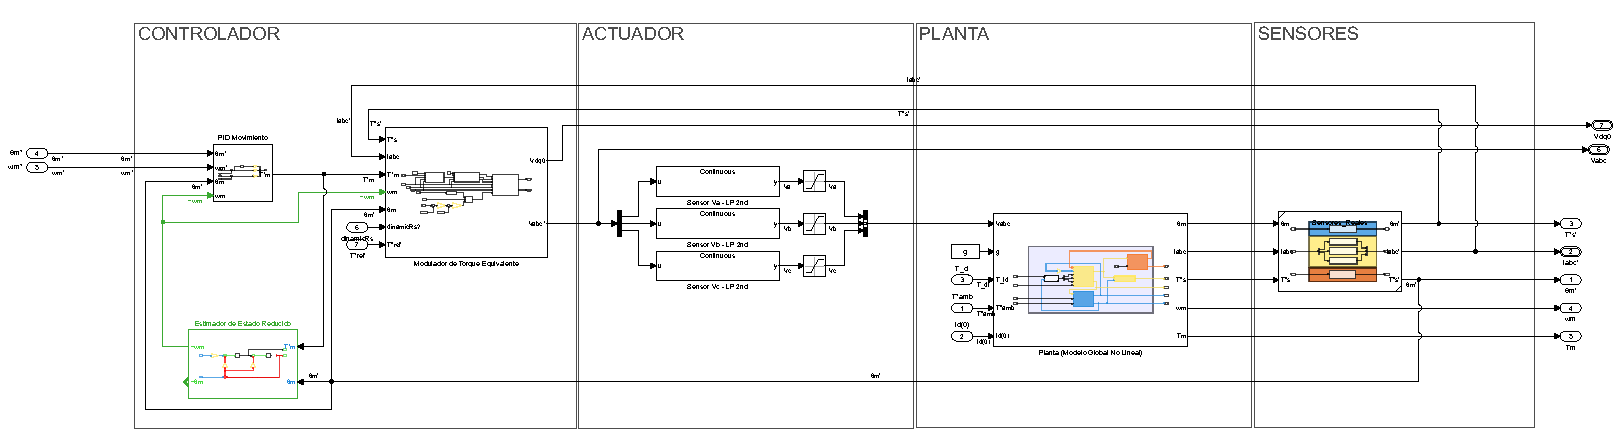
\includegraphics[width=\linewidth]{attachments/Sistema Final Continuo.pdf}
    \caption{Diagrama de bloques del sistema de control en tiempo continuo, integrado por el controlador de movimiento, el modulador de torque equivalente, el estimador de estado, el inversor trifásico, la planta no lineal y los sensores de realimentación.}
    \label{fig:sistema-final-continuo}
\end{figure}

Para la implementación digital, se consideran parte del controlador los bloques \textit{PID de Movimiento}, \textit{Modulador de Torque Equivalente} y \textit{Estimador de Estado de Orden Reducido}. El inversor, la planta y las dinámicas de los sensores se conservan en tiempo continuo. De este modo, la simulación representa la interacción de un controlador digital con un sistema físico continuo.

La interfaz de entrada al controlador se establece mediante el muestreo de las señales medidas. Para ello, se emplean bloques \textit{Zero-Order Hold} (ZOH), o retenedores de orden cero, que toman una muestra de cada señal y mantienen su valor hasta el siguiente instante de muestreo. En la interfaz de salida, la consigna de tensión calculada se conserva entre dos actualizaciones consecutivas.

La retención de la orden de actuación se sitúa sobre las señales que constituyen las entradas del inversor. Cuando este recibe consignas trifásicas, se mantiene constante el vector $\mathbf{v}_{abc}^{*}[k]$, calculado después de la transformación inversa de Park. Esta transformación forma parte del controlador y se evalúa con las muestras disponibles en cada actualización. En Simulink, una salida discreta ya conserva su valor entre instantes de ejecución; por tanto, la incorporación de un ZOH adicional a la salida puede utilizarse para hacer explícita esta interfaz, sin introducir un nuevo período de actualización.

Se adopta un único período de muestreo, constante y positivo, que define los instantes de ejecución:
\begin{equation}
    t_k=kT_s,
    \qquad k=0,1,2,\ldots,
    \qquad T_s>0
\end{equation}
donde $T_s$ se expresa en segundos.

Todos los cálculos del controlador se realizan con este período. Los bloques algebraicos, como ganancias, sumadores, compensaciones y transformaciones de coordenadas, conservan sus expresiones y operan sobre las muestras disponibles en cada instante $t_k$. En cambio, los estados internos del controlador requieren ecuaciones de actualización discretas.

En la estructura considerada, se discretizan el integrador del PID de movimiento y las ecuaciones dinámicas del estimador de estado. Si el selector de consignas se incorpora al algoritmo digital, su integrador también debe implementarse en tiempo discreto. Los integradores asociados a las dinámicas físicas de la planta permanecen continuos.

Para seleccionar $T_s$, se consideran las escalas temporales del diseño ideal de control: los polos del observador, ubicados en $-3200\;\mathrm{s^{-1}}$, y los polos de los lazos de corriente, ubicados en $-5000\;\mathrm{s^{-1}}$. Se adopta como referencia la dinámica más rápida entre ambas, correspondiente a los lazos de corriente:
\begin{equation}
    \omega_{\mathrm{ref}}=5000\;\mathrm{rad/s},
    \qquad
    f_{\mathrm{ref}}
    =\frac{\omega_{\mathrm{ref}}}{2\pi}
    \approx 795.77\;\mathrm{Hz}
\end{equation}

Por decisión de diseño, las dinámicas no ideales de los sensores y del actuador no se incluyen en la selección de esta frecuencia de referencia. Esta simplificación se limita al criterio inicial de muestreo y no implica eliminar dichas dinámicas del modelo de simulación. Su influencia debe considerarse al verificar la estabilidad y el desempeño del sistema discretizado.

El teorema de muestreo de Nyquist--Shannon establece una condición de reconstrucción para señales limitadas en banda, pero no garantiza por sí solo la estabilidad ni el desempeño de un sistema de control digital. En consecuencia, el período de ejecución también debe evaluarse considerando los efectos del muestreo, la retención y los retardos de cálculo sobre el lazo cerrado.

Como criterio inicial, se adopta una frecuencia de muestreo diez veces mayor que la frecuencia de referencia:
\begin{equation}
    f_s=10f_{\mathrm{ref}}
    \approx 7957.75\;\mathrm{Hz}.
\end{equation}
El período correspondiente resulta:
\begin{equation}
    T_s
    =\frac{1}{f_s}
    =\frac{2\pi}{10\omega_{\mathrm{ref}}}
    =\frac{2\pi}{10\cdot5000}
    \approx 1.2566\times10^{-4}\;\mathrm{s}
    =0.12566\;\mathrm{ms}
\end{equation}

Este valor se utiliza como punto de partida para la implementación discreta. Su validez debe comprobarse mediante la comparación con el controlador continuo y con implementaciones de menor período de muestreo, evaluando la estabilidad, el seguimiento de la consigna, el rechazo de perturbaciones y el esfuerzo de control.

Para implementar los integradores se utiliza la aproximación trapezoidal, asociada al método de Tustin. Sean $x(t)$ y $v(t)$ dos variables relacionadas mediante:
\begin{equation}
    \frac{dx(t)}{dt}=v(t).
\end{equation}
Al integrar entre dos instantes consecutivos, se obtiene:
\begin{equation}
    x(t_k)-x(t_{k-1})
    =\int_{t_{k-1}}^{t_k}v(\tau)\,d\tau
\end{equation}
La regla trapezoidal aproxima esta integral a partir del promedio de los valores de entrada en los extremos del intervalo:
\begin{equation}
    x[k]-x[k-1]
    \approx
    \frac{T_s}{2}
    \left(v[k]+v[k-1]\right).
\end{equation}
Por tanto, la ecuación de actualización del integrador discreto se expresa como:
\begin{equation}
    \boxed{
    x[k]=x[k-1]
    +\frac{T_s}{2}
    \left(v[k]+v[k-1]\right)
    }
\end{equation}

Esta implementación requiere almacenar la entrada y la salida anteriores, lo que se realiza mediante bloques \textit{Unit Delay}, configurados con período de muestreo $T_s$. Las condiciones iniciales de estas memorias deben establecerse de acuerdo con el estado inicial del integrador y con la convención de actualización utilizada, verificando especialmente el valor de la primera muestra.

La Figura~\ref{fig:equivalencia-integrador-tustin} presenta el bloque integrador continuo y su implementación discreta mediante la aproximación trapezoidal.

\begin{figure}[!htbp]
    \centering
    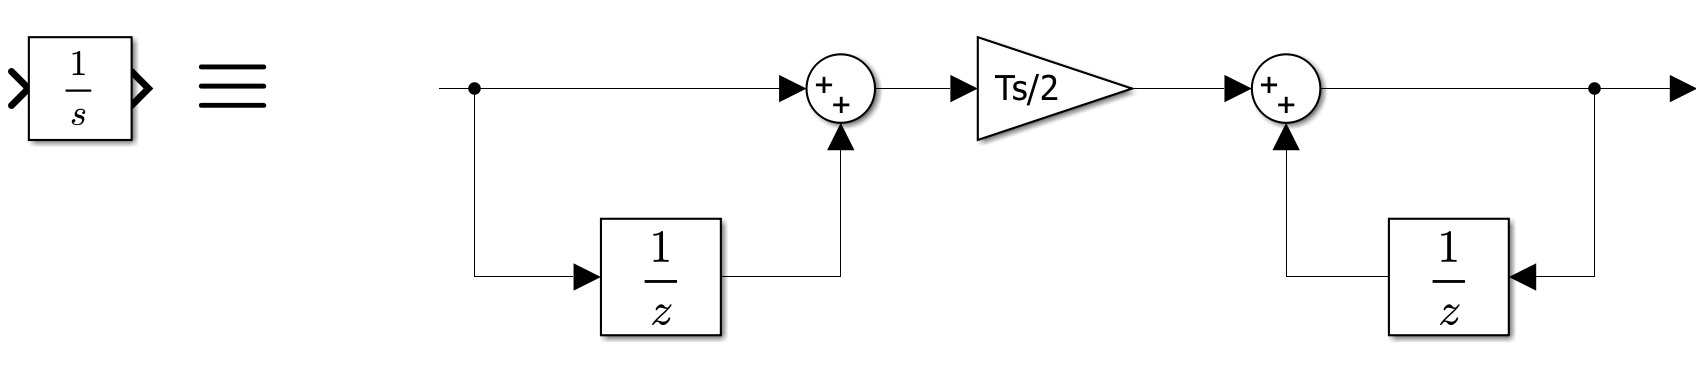
\includegraphics[width=\linewidth]{attachments/Integrador de Tustin.png}
    \caption{Implementación discreta del integrador mediante el método de Tustin, utilizando sumadores, una ganancia $T_s/2$ y memorias de una muestra.}
    \label{fig:equivalencia-integrador-tustin}
\end{figure}

A partir de esta estructura, se sustituyen los integradores continuos del PID de movimiento y del estimador de estado por sus implementaciones discretas. En el PID, la acción asociada a la derivada se calcula mediante el error de velocidad, por lo que no se requiere incorporar un derivador numérico de la posición.

Las Figuras~\ref{fig:pid-movimiento-discreto} y~\ref{fig:estimador-estado-discreto} presentan las estructuras resultantes. En el estimador, la dependencia de la actualización trapezoidal respecto de la entrada actual exige comprobar la resolución de sus realimentaciones internas y la posible aparición de lazos algebraicos.

\begin{figure}[!htbp]
    \centering
    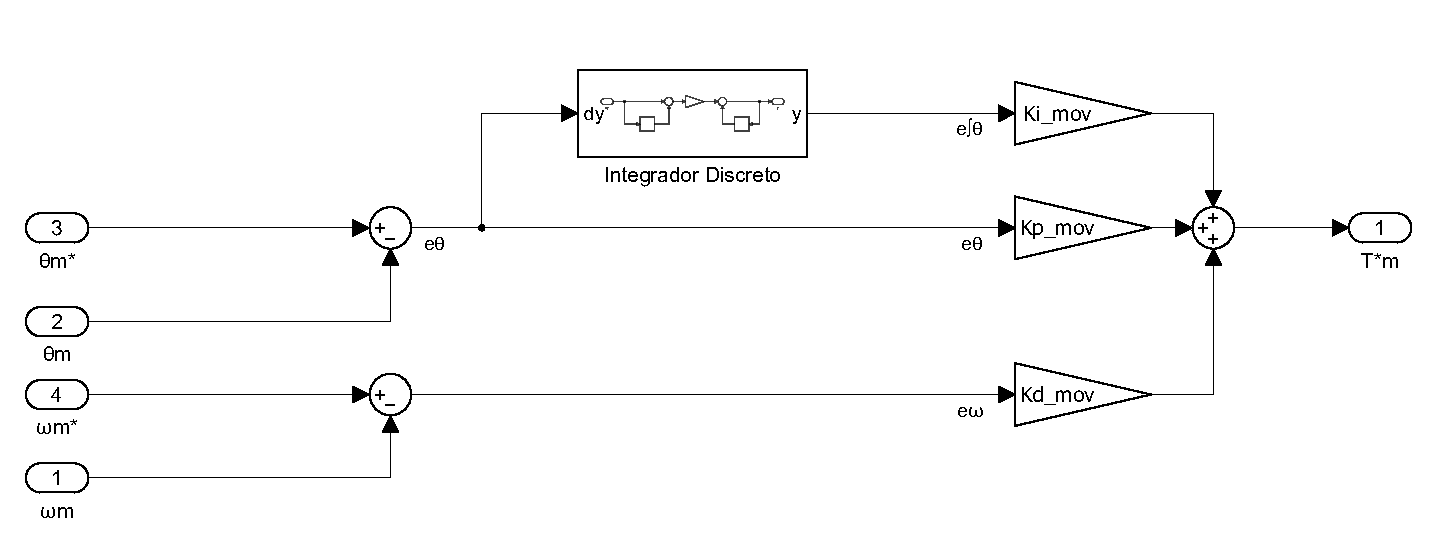
\includegraphics[width=\linewidth]{attachments/PID Movimiento Discreto.pdf}
    \caption{Implementación discreta del PID de movimiento, con integración del error de posición mediante Tustin y acción derivativa calculada a partir del error de velocidad.}
    \label{fig:pid-movimiento-discreto}
\end{figure}

\begin{figure}[!htbp]
    \centering
    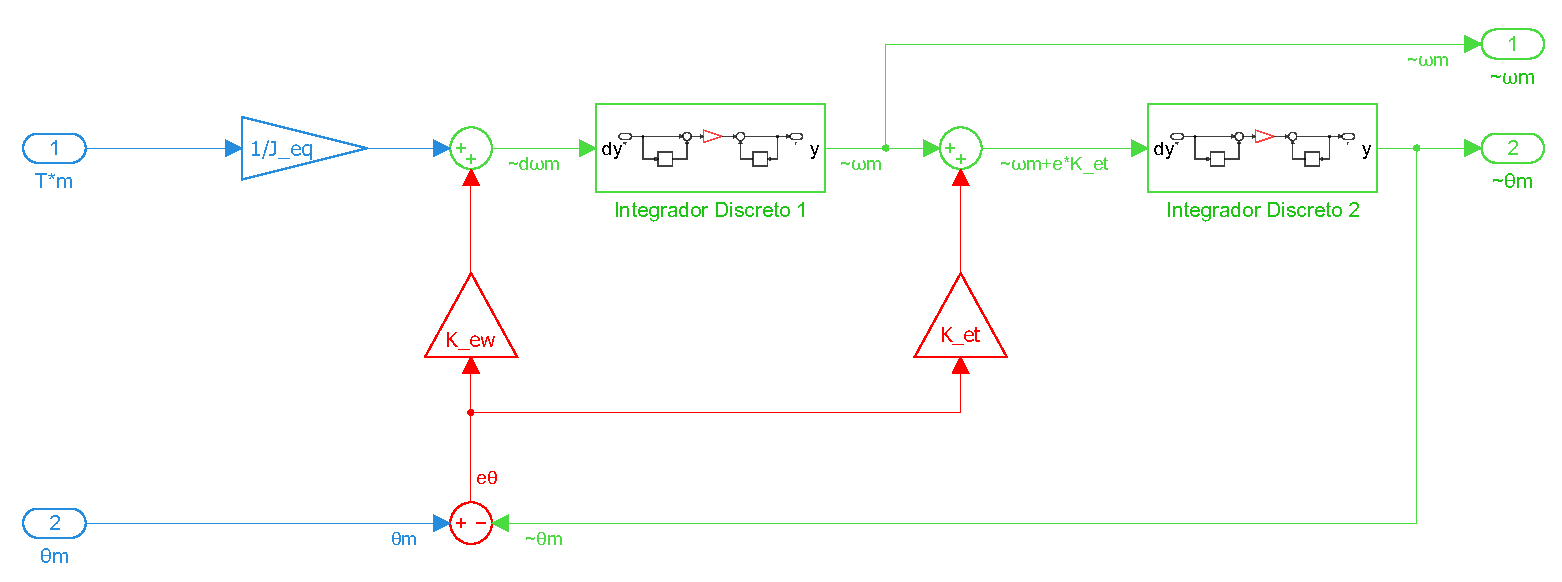
\includegraphics[width=\linewidth]{attachments/Estimador de Estado Reducido Discreto.pdf}
    \caption{Implementación discreta del estimador de posición y velocidad angular del motor, con actualización de sus estados mediante integradores de Tustin.}
    \label{fig:estimador-estado-discreto}
\end{figure}

Finalmente, la Figura~\ref{fig:sistema-final-discretizado} presenta la integración del controlador discreto con el inversor, la planta y los sensores continuos, junto con las interfaces de muestreo y retención correspondientes.

\begin{figure}[!htbp]
    \centering
    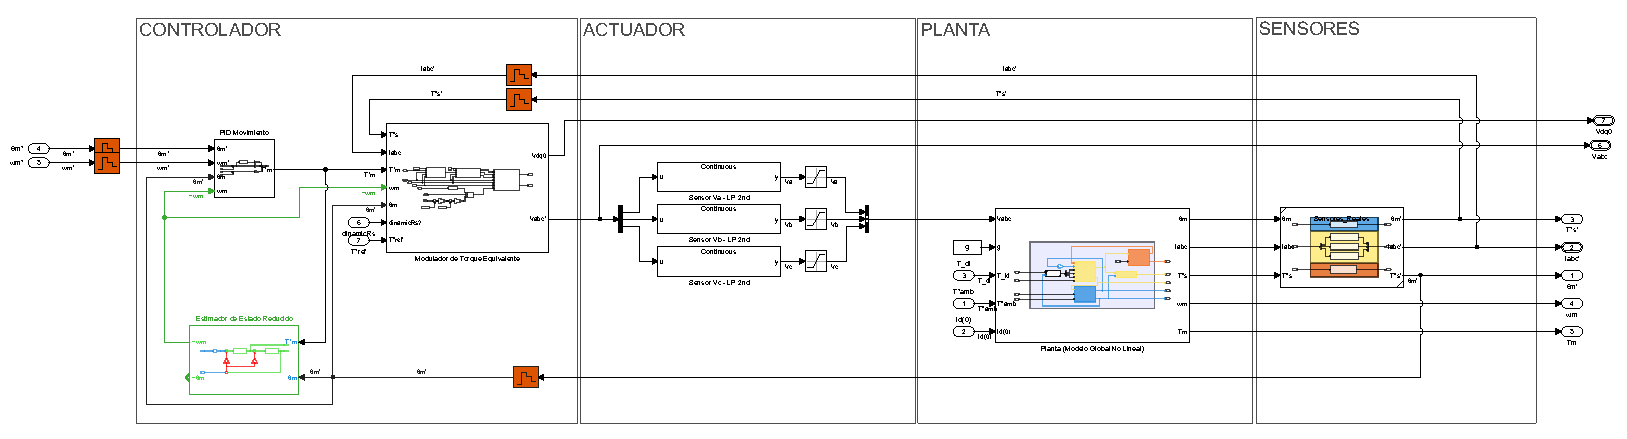
\includegraphics[width=\linewidth]{attachments/Sistema Final Discretizado.pdf}
    \caption{Sistema de control con controlador discreto de período $T_s=0.12566\;\mathrm{ms}$, interfaces de muestreo y retención, y modelos continuos del inversor, la planta y los sensores.}
    \label{fig:sistema-final-discretizado}
\end{figure}


\clearpage
% ============================================================================= %
\subsection{Codificación del software de control}

En este apartado se implementa el algoritmo de control digital mediante un bloque \texttt{MATLAB Function} dentro del modelo de Simulink. Para ello, las operaciones de los subsistemas del controlador se expresan mediante una función principal y un conjunto de subfunciones que representan el PID de movimiento, el estimador de estado, el modulador de torque equivalente, los reguladores de corriente, las compensaciones no lineales, las transformadas de Park y los integradores discretos.

La función principal recibe las referencias de posición y velocidad del eje motor, las mediciones de posición, corrientes y temperatura, las señales de configuración y una estructura denominada \texttt{p\_control}. Esta estructura reúne las ganancias, los parámetros físicos utilizados por el algoritmo y el período de muestreo $T_s$. Dentro de las funciones se utiliza el nombre \texttt{parametros} para acceder a sus campos.

La única salida de actuación es el vector de consignas de tensión trifásica:
\begin{equation}
    \mathbf{v}_{abc}^{*}[k]
    =
    \begin{bmatrix}
        v_a^{*}[k] &
        v_b^{*}[k] &
        v_c^{*}[k]
    \end{bmatrix}^{T},
\end{equation}
que se entrega al inversor. Las salidas restantes se conservan para diagnóstico y registro de las variables internas; no constituyen acciones adicionales sobre la planta. Las consignas de tensión deben distinguirse de las tensiones efectivamente aplicadas al motor, que dependen de la dinámica y de la saturación del inversor.

Se adopta una ejecución secuencial: en cada instante de muestreo, primero se actualiza la integral del error de posición y se calcula el torque de movimiento utilizando la velocidad estimada anterior, $\hat{\omega}_m[k-1]$. Luego se actualiza el observador, cuya corrección utiliza el error $\theta'_m[k]-\hat{\theta}_m[k-1]$. Finalmente, el modulador calcula las consignas de tensión empleando la velocidad estimada actualizada.

% Esta organización introduce retardos de una muestra en las realimentaciones mencionadas respecto de la implementación simultánea. Por tanto, aunque se conserva la regla trapezoidal para la acumulación de los integradores, el algoritmo resultante presenta una dinámica diferente, cuyo desempeño debe verificarse mediante simulación.

El almacenamiento entre ejecuciones se realiza mediante una variable persistente que contiene seis valores: la integral del error de posición, el error de posición, la velocidad estimada, su derivada, la posición estimada y su derivada. Al comenzar cada llamada se recuperan los valores anteriores y, al finalizar, se almacenan los resultados actuales. La entrada \texttt{reset} permite reiniciar estas memorias antes de efectuar el cálculo de la muestra correspondiente.

La implementación se presenta en el Listado~\ref{lst:controlador-digital}.

\begin{lstlisting}[
    style=codigoMATLAB,
    caption={Implementación secuencial del controlador digital mediante una función principal y subfunciones.},
    label={lst:controlador-digital}
]
function [vabc, vdq0, torque_mov, omega_hat, theta_hat, ...
          idq0, iq_ref, Rs] = controlador_digital( ...
    theta_ref, omega_ref, theta, iabc, temperatura, ...
    resistencia_dinamica, temperatura_ref, reset, p_control)
%#codegen
% Calcula una muestra del controlador digital secuencial.
% Entradas: referencias motor, mediciones, selector de Rs, reset y parametros.
% Salida de actuacion: vabc [3x1, V]. Las demas salidas son diagnosticos.

parametros = p_control;

persistent memoria
if isempty(memoria)
    memoria = zeros(6,1);
end

if reset ~= 0
    memoria = zeros(6,1);
end

anterior = memoria;

error_posicion = theta_ref - theta;

integral_error = Integrador_Discreto( ...
    error_posicion, anterior(1), anterior(2), parametros.Ts);

omega_anterior = anterior(3);

torque_mov = PID_de_Movimiento( ...
    theta_ref, omega_ref, theta, omega_anterior, ...
    integral_error, parametros);

[omega_hat, theta_hat, deriv_omega, deriv_theta] = ...
    Estimador_de_Estado_de_Orden_Reducido( ...
        torque_mov, theta, anterior, parametros);

[vabc, vdq0, idq0, iq_ref, Rs] = ...
    Modulador_de_Torque_Equivalente( ...
        torque_mov, omega_hat, theta, iabc, temperatura, ...
        resistencia_dinamica, temperatura_ref, parametros);

memoria = [integral_error; error_posicion; ...
           omega_hat; deriv_omega; theta_hat; deriv_theta];
end


function torque = PID_de_Movimiento( ...
    theta_ref, omega_ref, theta, omega, integral_error, parametros)
% Calcula el torque de movimiento mediante acciones P, I y D.
% Entradas: posiciones [rad], velocidades [rad/s], integral [rad s] y parametros.
% Salida: torque [N m], consigna referida al eje motor.

torque = parametros.Ki_mov*integral_error ...
       + parametros.Kp_mov*(theta_ref-theta) ...
       + parametros.Kd_mov*(omega_ref-omega);
end


function [omega_hat, theta_hat, deriv_omega, deriv_theta] = ...
    Estimador_de_Estado_de_Orden_Reducido( ...
        torque_mov, theta_medida, memoria_anterior, parametros)
% Actualiza secuencialmente las estimaciones de velocidad y posicion.
% Entradas: torque [N m], posicion medida [rad], memorias previas y parametros.
% Salidas: estimaciones [rad/s, rad] y derivadas [rad/s^2, rad/s].

omega_anterior       = memoria_anterior(3);
deriv_omega_anterior = memoria_anterior(4);
theta_anterior       = memoria_anterior(5);
deriv_theta_anterior = memoria_anterior(6);

error_estimacion = theta_medida - theta_anterior;

deriv_omega = torque_mov/parametros.J_eq ...
            + parametros.K_ew*error_estimacion;

omega_hat = Integrador_Discreto( ...
    deriv_omega, omega_anterior, ...
    deriv_omega_anterior, parametros.Ts);

deriv_theta = omega_hat ...
            + parametros.K_et*error_estimacion;

theta_hat = Integrador_Discreto( ...
    deriv_theta, theta_anterior, ...
    deriv_theta_anterior, parametros.Ts);
end


function [vabc, vdq0, idq0, iq_ref, Rs] = ...
    Modulador_de_Torque_Equivalente( ...
        torque, omega, theta, iabc, temperatura, ...
        dinamica, temperatura_ref, parametros)
% Integra la conversion de torque, los lazos de corriente y el desacoplamiento.
% Entradas: torque, velocidad estimada, mediciones y configuracion.
% Salidas: tensiones abc/dq0 [V], corrientes dq0 [A], iq_ref [A] y Rs [ohm].

idq0 = Transformada_Directa_de_Park( ...
    iabc, parametros.Pp*theta);

Rs = Calculo_de_Resistencia( ...
    temperatura, dinamica, temperatura_ref, parametros);

iq_ref = Modulador_de_Torque( ...
    torque, omega, theta, idq0(1), parametros);

virtual = Lazo_de_Corriente( ...
    [0; iq_ref; 0], idq0, parametros);

vdq0 = Modulador_de_Tension( ...
    virtual, idq0, omega, Rs, parametros);

vabc = Transformada_Inversa_de_Park( ...
    vdq0, parametros.Pp*theta);
end


function iq_ref = Modulador_de_Torque( ...
    torque, omega, theta, id, parametros)
% Compensa friccion y gravedad y convierte torque a corriente.
% Entradas: torque [N m], omega [rad/s], theta [rad], id [A] y parametros.
% Salida: iq_ref [A], referencia de corriente en cuadratura.

torque_compensado = torque ...
    + parametros.b_eq*omega ...
    + (parametros.k_l*parametros.g/parametros.r) ...
      *sin(theta/parametros.r);

constante_torque = (3/2)*parametros.Pp ...
    *(parametros.lambda + (parametros.L_d-parametros.L_q)*id);

iq_ref = torque_compensado/constante_torque;
end


function virtual = Lazo_de_Corriente( ...
    referencia, medida, parametros)
% Aplica reguladores proporcionales en los ejes d, q y cero.
% Entradas: referencia y medida [3x1, A], en orden d/q/0, y parametros.
% Salida: virtual [3x1, V], tensiones antes de la compensacion electrica.

virtual = [ ...
    parametros.Rd*(referencia(1)-medida(1));
    parametros.Rq*(referencia(2)-medida(2));
    parametros.R0*(referencia(3)-medida(3))];
end


function vdq0 = Modulador_de_Tension( ...
    virtual, idq0, omega, Rs, parametros)
% Compensa resistencia, acoplamientos dq y fuerza contraelectromotriz.
% Entradas: virtual [V], idq0 [A], omega [rad/s motor], Rs [ohm] y parametros.
% Salida: vdq0 [3x1, V], tensiones compensadas en orden d/q/0.

omega_e = parametros.Pp*omega;

vdq0 = [ ...
    virtual(1) + Rs*idq0(1) ...
        - omega_e*parametros.L_q*idq0(2);
    virtual(2) + Rs*idq0(2) ...
        + omega_e*(parametros.L_d*idq0(1)+parametros.lambda);
    virtual(3) + Rs*idq0(3)];
end


function dq0 = Transformada_Directa_de_Park(abc, theta_e)
% Transforma abc a dq0 con amplitud invariante: d seno, q coseno.
% Entradas: abc [3x1] y angulo electrico theta_e [rad].
% Salida: dq0 [3x1], con las mismas unidades que abc.

angulos = [theta_e; theta_e-2*pi/3; theta_e+2*pi/3];

dq0 = [ ...
    (2/3)*sum(sin(angulos).*abc);
    (2/3)*sum(cos(angulos).*abc);
    (abc(1)+abc(2)+abc(3))/3];
end


function abc = Transformada_Inversa_de_Park(dq0, theta_e)
% Transforma dq0 a abc con la convencion de la transformada directa.
% Entradas: dq0 [3x1] y angulo electrico theta_e [rad].
% Salida: abc [3x1], con las mismas unidades que dq0.

angulos = [theta_e; theta_e-2*pi/3; theta_e+2*pi/3];

abc = sin(angulos)*dq0(1) ...
    + cos(angulos)*dq0(2) ...
    + ones(3,1)*dq0(3);
end


function valor = Integrador_Discreto( ...
    entrada, valor_previo, entrada_previa, Ts)
% Acumula la integral mediante la regla trapezoidal.
% Entradas: entrada actual/anterior, integral previa y Ts [s].
% Salida: valor, integral actual.

valor = valor_previo + (Ts/2)*(entrada+entrada_previa);
end


function Rs = Calculo_de_Resistencia( ...
    temperatura, dinamica, temperatura_ref, parametros)
% Selecciona la temperatura de compensacion y calcula la resistencia.
% Entradas: temperaturas [grados Celsius], selector y parametros.
% Salida: Rs [ohm], resistencia de compensacion.

if dinamica > parametros.umbral_Rs
    temperatura_usada = temperatura;
else
    temperatura_usada = temperatura_ref;
end

Rs = parametros.R_sREF ...
    *(1 + parametros.alpha_Cu ...
    *(temperatura_usada-parametros.T_sREF));
end
\end{lstlisting}

La estructura modular permite identificar la correspondencia entre las operaciones del código y los subsistemas de Simulink. Las funciones auxiliares no almacenan estados propios: las memorias de los integradores se administran exclusivamente en la función principal. De esta manera, cada subsistema se evalúa una vez por período de muestreo y la actualización de los estados se realiza al finalizar el cálculo de la muestra.

\clearpage
% ============================================================================= %
\section{Conclusiones}
A lo largo del estudio, se fue complejizando el estudio de aplicación de control de movimiento para un brazo manipulador de un grado de libertad accionado por un motor síncrono de imanes permanentes (PMSM): desde el modelo matemático con ecuaciones diferenciales que responden a los fenómenos mecánicos, electromagnéticos y térmicos hasta el diseño discretizado del controlador que toma consignas y se asegura que sean implementadas correctamente.

Este estudio fue realizado apoyándose fuertemente en las herramientas de modelado y simulación MATLAB y Simulink de Mahtworks, por lo que los resultados obtenidos pueden no ser reflejo perfecto de los fenómenos que ocurren en la realidad, producto de las limitaciones de los modelos matemáticos, los limitantes del software y las diferencias introducidas cada vez que se planteaba una hipótesis. Aún así, el desarrollo de control basado en modelos permite al ingeniero estudiar la aplicación en gran profundidad sin necesidad de interactuar con el sistema real, evitando tiempos de experimentación y costos por errores durante dicha experimentación.

En cuanto a la aplicación impuesta: 

\paragraph{Espacio virtual}
La transformada de Park permitió expresar las variables trifásicas
del estator en un marco de referencia ligado al rotor. Esta
representación hizo explícitos los acoplamientos entre las variables
eléctricas y mecánicas y facilitó el diseño de las leyes de control
para las corrientes de los ejes directo y en cuadratura.

\paragraph{Modelos LTI y LPV}
El modelo LPV permitió estudiar la dinámica local de la planta en
distintas condiciones de operación. A su vez, la compensación por
realimentación no lineal y las hipótesis de simplificación permitieron
obtener un modelo LTI equivalente para el diseño. Sobre este modelo
se aplicaron herramientas de análisis de polos, estudio de estabilidad del sistema y estudio de controlabilidad y observabilidad.

\paragraph{Modulación de torque y corriente}
Se diseñó un modulador de torque equivalente con una estructura
en cascada. La etapa de torque incorpora las compensaciones de
gravedad y fricción viscosa y convierte la consigna de torque en
una referencia de corriente. El lazo interno regula las corrientes,
y el modulador de tensión genera las tensiones trifásicas mediante
la compensación de los acoplamientos eléctricos. Esta estructura
permite que el lazo externo de movimiento actúe sobre la posición
y la velocidad del brazo a través de la consigna de torque.

\paragraph{Controlador de movimiento}
Se diseñó un controlador PID de movimiento y se calcularon sus
ganancias mediante asignación de polos. Los polos del lazo de
movimiento se eligieron para obtener una respuesta más lenta que
la del lazo interno de corriente. Esta separación de escalas permite
que la corriente responda con rapidez a las demandas de torque
del controlador de movimiento.

\paragraph{Estimador de estado}
Se implementó un estimador de estado de orden reducido para
obtener la velocidad angular del motor a partir de la posición
medida. La velocidad estimada se utilizó en la realimentación
del accionamiento. En las condiciones nominales de diseño,
la ubicación de los polos del estimador da lugar a un error
de estimación que converge exponencialmente a cero.

\paragraph{Cumplimiento de la consigna}
El perfil trapezoidal de posición presenta cambios instantáneos
en la velocidad de referencia. En simulación, el intento de seguir
esas transiciones produjo demandas de tensión del orden de cientos
de voltios y picos de corriente superiores a $30\,\mathrm{A}$,
por encima de los límites del accionamiento. Para reducir estas
exigencias, se suavizaron las transiciones de velocidad y se
obtuvieron perfiles de aceleración de forma aproximadamente
triangular.

\paragraph{Análisis térmico}
El análisis térmico mostró que un seguimiento satisfactorio
de la consigna puede coexistir con temperaturas superiores al
límite admisible del estator. Por lo tanto, la evaluación del
accionamiento debe considerar tanto la respuesta de movimiento
como la evolución de la temperatura bajo las condiciones de
carga y los ciclos de trabajo previstos.

\paragraph{Control discretizado}
Se discretizó el controlador y se implementó tanto mediante
bloques de Simulink como mediante un bloque \texttt{MATLAB Function}.
Este desarrollo permitió expresar el algoritmo como una secuencia
de cálculos y actualizaciones de estado ejecutados en cada período
de muestreo, tal como requiere una implementación en hardware digital.

\paragraph{Resultado del control}
En las simulaciones se obtuvo seguimiento de posición del brazo
de un grado de libertad con la consigna suavizada para las masas
de carga ensayadas. El suavizado conservó los desplazamientos
previstos y redujo las exigencias de aceleración en las transiciones.

\clearpage
% ============================================================================= %


%% References using BibTeX
%% Make sure to compile with: pdflatex -> bibtex -> pdflatex -> pdflatex
\nocite{julian2026guia,astrom2020feedback,ogata2010control}
\bibliographystyle{plain}
\bibliography{references}

\end{document}
